\documentclass[12pt,twoside,a4paper,english,french]{book} %fleqn % use larger type; default would be 10pt
% Les langues (français et anglais) sont passées directement à babel et à tous les autres packages qui pourraient en avoir besoin.
% C'est la même chose pour a4paper, geometry hérite cette option.
% La dernière langue spécifiée sera la langue principale.

%__________________________Packages____________________________________
\usepackage{amsmath}		% pour les symboles de maths
\usepackage{graphicx}	% pour afficher des figures
\usepackage{amssymb}		% encore des maths
\usepackage{eurosym}		%symbole euro
\usepackage{lscape}							% passer des éléments en position paysage
\usepackage{longtable}						% Table sur plusieurs pages
\usepackage{multirow}							% Tables avec cellules fusionnées Columns spanning multiple rows https://en.wikibooks.org/wiki/LaTeX/Tables
\usepackage{enumitem}							% pour gérer les listes avec paramètres [noitemsep,topsep=0pt,parsep=0pt,partopsep=0pt]
\usepackage{color}							% pour la couleur
%\usepackage[dvipsnames]{xcolor}			% alternative  pour la couleur, 
\usepackage[skins, breakable]{tcolorbox}	%boite remarques, commentaires, exemples
\usepackage{makeidx}					%pour faire un index
\usepackage{tikz}
\usepackage[raccourcis]{fast-diagram} %
%\usepackage{include}

% ordre des packages ! varioref ; hyperref ; cleverref http://tex.stackexchange.com/questions/139459/vref-and-input-command

\usepackage[utf8]{inputenc}	% pour poser proprement le type de code
\usepackage[T1]{fontenc}		% nécessaire pour le package babel [T1]
\usepackage{textcomp} 			%test symbols
\usepackage{lmodern}
\usepackage[frenchb]{babel}	% pour pouvoir écrire directement avec les accents [frenchb]
%\usepackage[top=3cm, bottom=3cm, inner=3cm, outer=3cm]{geometry} % marges, dimensions de la page...

\usepackage{csquotes}
%\SetBlockThreshold{52}			% défini le nombre de ligne avant passage en bloc
\usepackage[backend=biber, backref, sorting=none, style=numeric-comp, doi=false, url=false, isbn=false, maxcitenames=1]{biblatex}
%\usepackage[backend=biber, backref, sorting=none, style=numeric-comp, doi=false, url=false, isbn=false, maxcitenames=2, eprint=false]{biblatex}
	
\addbibresource{zotero_selec_all_biblatex.bib}
%\usepackage[french]{varioref}						% il faut appeler \vref et pas \ref
%\usepackage{cleveref}						% faire le beau gosse avec ``ci-contre'',``page suivante''...localisation et type de contenu

\usepackage[colorlinks=true, linkcolor=red, citecolor=blue, pdftex]{hyperref} % hyperlien pagebackref=true, 

\usepackage{caption}
\usepackage{subcaption}
\usepackage[all]{hypcap}					% pour les hyperlien vers les figures sur la figure et non sur la légende
\usepackage{wrapfig} 						%figure entourée de texte
\usepackage{listings} %mettre du code

%____________________Commandes______________________________________
%\definecolor{bleuclair}{rgb}{0.7, 0.7, 1.0}
%\definecolor{rosepale}{rgb}{1.0, 0.7, 1.0}

% Barrer du texte : \barre{texte barré}
\newlength{\textlarg}
\newcommand{\barre}[1]{%
   \settowidth{\textlarg}{#1}
   #1\hspace{-\textlarg}\rule[0.5ex]{\textlarg}{0.5pt}}

% gestion de la profondeur de numérotation et d'affichage en TOC
\setcounter{tocdepth}{2}
\setcounter{secnumdepth}{2}

%_____________________Glossaire____________________________________
\usepackage[xindy,acronyms,toc,section=chapter]{glossaries}
\makeglossaries
\setglossarystyle{listhypergroup}
\renewcommand*{\glstextformat}[1]{%
\textcolor{magenta}{#1}}% <-- passer en vert ?

\loadglsentries{glossaire}

%_______________________Mes boites_____________________________

%Lectures de figures_______
\newcommand{\figbox}[1] {
\begin{tcolorbox}[width=\linewidth, boxsep=2pt, left=2pt, right=2pt, top=2pt, breakable] #1 \end{tcolorbox}}
%Exemples__________________
\newcommand{\exbox}[1] {
\begin{tcolorbox}[colframe=green!50!white, colback=green!10!white, width=\linewidth, boxsep=2pt, left=2pt, right=2pt, top=2pt, arc=3mm, breakable] #1 \end{tcolorbox}}
%Notions Clefs_____________
\newcommand{\keybox}[1]{\begin{tcolorbox}[colframe=red!50!white, width=\linewidth,boxsep=2pt, left=2pt, right=2pt, top=2pt, arc=-1mm, breakable] #1 \end{tcolorbox}}

%listing above text

% Metadonnées____________________________________________________
%\title{Fondations de l'Évaluation Holistique Opérationnelle\\Re-conception méthodologique de l'évaluation de la soutenabilité par la pensée en cycle de vie} % et l'artificialisme}
\title{Contribution à la re-conception méthodologique de l'évaluation de la soutenabilité par la pensée en cycle de vie, via l'intégration explicite du jugement, le traitement de la multi-dimensionnalité et l'approche alternative libre des données.}
\author{Rudy Patard}
\date{\today}

%____________________________________________
%\includeonly{recherche_libre}
%____________________________________________

\begin{document}
\frontmatter % Numerotation des pages en chiffres romains
% A mettre au début du document, pour ne pas avoir 1, 2, i, ii, 1, 2, 3 ... (éviter la répétition)
\begin{titlepage}

  \thispagestyle{empty} %% To center the title page, and do not have a numbered page
  \newcommand{\HRule}{\rule{\linewidth}{0.5mm}} % Defines a new command for the horizontal lines, change thickness here
  \center % Center everything on the page
  % HEADING SECTIONS
%  UNIVERSITE LILLE NORD-DE-FRANCE
%  \begin{figure}
%  \begin{subfigure}[b]{0.5\textwidth}
%  \href{http://umet.univ-lille1.fr}{\includegraphics[width=0.5\textwidth]{/home/rudy/Documents/rudy/01_These/11_production/01_COMMUNICATION/01_RAPPORT/Memoire/img/umet.png}}
%  \end{subfigure}
%  \begin{subfigure}[b]{0.5\textwidth}
%  \begin{flushright}
%  \href{http://www.univ-lille1.fr}{\includegraphics[width=0.5\textwidth]{/home/rudy/Documents/rudy/01_These/11_production/01_COMMUNICATION/figures_extraites/Logos/UL1-WEB-2014.png/UL1-WEB-2014.png}}
%  \end{flushright}
%  \end{subfigure}
%  \end{figure}
%  \vspace{-2cm}
%% 
%  \begin{minipage}{0.42\textwidth}
%  \begin{flushleft} \large
%          \href{http://umet.univ-lille1.fr}{\includegraphics[width=0.5\textwidth]{/home/rudy/Documents/rudy/01_These/11_production/01_COMMUNICATION/01_RAPPORT/Memoire/img/umet.png}}
%        \end{flushleft}
%    \begin{flushright} \large
%      \href{http://www.univ-lille1.fr}{\includegraphics[width=0.5\textwidth]{/home/rudy/Documents/rudy/01_These/11_production/01_COMMUNICATION/figures_extraites/Logos/UL1-WEB-2014.png/UL1-WEB-2014.png}}
%    \end{flushright}
%  \end{minipage}\\ %[3cm]
%  \begin{minipage}{0.42\textwidth}
%      
%    \end{minipage}\\ [1cm]
%\begin{figure}
%  \begin{subfigure}[b]{0.25\textwidth}
%  \begin{center}
%  \href{http://edsmre.univ-lille1.fr}{\includegraphics[width=0.5\textwidth]{/home/rudy/Documents/rudy/01_These/11_production/01_COMMUNICATION/figures_extraites/Logos/EDSMRE-104_logo.pdf}}
%  \end{center}
%  \end{subfigure}
%  \begin{subfigure}[b]{0.7\textwidth} \large
%  École Doctorale - 104 \\Sciences de la Matière, du Rayonnement\\et de l'Environnement
%  \end{subfigure}
%\end{figure}
%\vspace{-2cm}
  % TITLE SECTION
  %\href{http://umet.univ-lille1.fr}{\includegraphics[width=4cm]{/home/rudy/Documents/rudy/01_These/11_production/01_COMMUNICATION/01_RAPPORT/Memoire/img/umet.png}}~~~~
  %\href{http://edsmre.univ-lille1.fr}{\includegraphics[width=3cm]{/home/rudy/Documents/rudy/01_These/11_production/01_COMMUNICATION/figures_extraites/Logos/EDSMRE-104_logo.pdf}}~~~
  %\href{http://www.univ-lille1.fr}{\includegraphics[width=4cm]{/home/rudy/Documents/rudy/01_These/11_production/01_COMMUNICATION/figures_extraites/Logos/UL1-WEB-2014.png/UL1-WEB-2014.png}}\\
  École Doctorale - à déterminer\\%104 \\Sciences de la Matière, du Rayonnement
%  \\  et de l'Environnement
%  \HRule \\[0.3cm]
  { \large \bfseries
%  Fondations de l'Évaluation Holistique Opérationnelle\\Re-conception méthodologique de l'évaluation de la soutenabilité par la pensée en cycle de vie et l'artificialisme %, l'intégration explicite du jugement de valeurs et la recherche libre
Re-conception méthodologique de l'évaluation de la soutenabilité par la pensée en cycle de vie\\
ou\\
Contribution à la re-conception méthodologique de l'évaluation de la soutenabilité par la pensée en cycle de vie, via l'intégration explicite du jugement, le traitement de la multi-dimensionnalité et l'approche alternative libre des données.\\
ou\\
Fondations de l'Évaluation Holistique Opérationnelle\\Re-conception méthodologique de l'évaluation de la soutenabilité par la pensée en cycle de vie
%Contribution à la re-conception méthodologique de l'évaluation de la soutenabilité par la pensée en cycle de vie, via l'intégration explicite du jugement, le traitement de la multi-dimensionnalité. % et l'approche alternative libre des données.
%   Thèse de doctorat
   }\\[0.1cm] % Title of your document
  \HRule \\[0.3cm]
  { %\large
  \bfseries
	Thèse pour l'obtention du grade de\\
	Docteur de \\%l’université de Lille 1\\
	\emph{Spécialités~:}\\
%	Conception. Interdisciplinarité de l'évaluation de la soutenabilité.
	}
\emph{Défendue par~:} %\\
\href{mailto:rudy.patard@gmail.com}{Rudy \textsc{Patard}}\\ % Your name
%\address{
%UMET, UMR CNRS 8207, 
%Universit\'e Lille~1, \\
%59655 Villeneuve D'Ascq, France \\[.5cm]
%E-mail: rudy.patard@ed.univ-lille1.fr\\
%}
%~\\[.5cm]
  \emph{Composition du Jury~:}\\[0.2cm]
%  {\small
%  \begin{tabular}{p{4.5cm} p{3.8cm} p{3.5cm}}%p{4cm} p{4cm} p{4cm}
%%  \hline
%%    Angélique Léonard
%%        Peggy Zwolinski
%%Peggy ZWOLINSKI
%%Grenoble Universities
%%Peggy.zwolinski@g-scop.inpg.fr
%%+33 4 7682 7028
%%        Anne Perwuelz
%%    Nicolas Perry
%%    Stéphane Le Pochat
%	\href{mailto:a.leonard@ulg.ac.be}{Pr. Angélique \textsc{Léonard}} & Université de Liège, LGC. génie chimique &  ------\\
%	\href{mailto:peggy.zwolinski@g-scop.inpg.fr}{Pr. Peggy \textsc{Zwolinski}} & Université Grenoble Alpes, G-SCOP & ------ \\
%	\href{mailto:anne.perwuelz@ensait.fr}{Pr. Anne \textsc{Perwuelz}} & ENSAIT, GEMTEX, Roubaix & ------ \\
%	\href{mailto:s.lepochat@evea-conseil.com}{Stéphane \textsc{Le Pochat}} & EVEA-Conseil SAS. & ------ \\
%	\href{mailto:n.perry@i2m.u-bordeaux1.fr}{Pr. Nicolas \textsc{Perry}} & Université de Bordeaux, Dép. IMC, I2M UMR~5295 & ------ \\
%	\href{mailto:david.balloy@univ-lille1.fr}{Pr. David \textsc{Balloy}} & Université de Lille 1, UMET & Directeur de thèse \\ % Supervisor's Name
%	\href{mailto:ion-cosmin.gruescu@univ-lille1.fr}{Ion-Cosmin \textsc{Gruescu}} & Université de Lille~1, LML FRE3723 & Encadrant \\
%	\href{mailto:anne-lise.cristol@centralelille.fr}{Anne-Lise \textsc{Cristol}}  & École Centrale de Lille, LML FRE3723 & Encadrante \\
%	}
%  \end{tabular}\\[.2cm]
  % AUTHOR SECTION

\end{titlepage}
\thispagestyle{empty}
\cleardoublepage
{\large \bfseries
Contribution à la re-conception méthodologique de\\l'évaluation de la soutenabilité par la pensée en cycle de vie, via l'intégration explicite du jugement, le traitement de la multi-dimensionnalité et l'approche alternative libre des données.
%Fondations de l'Évaluation Holistique Opérationnelle\\Re-conception méthodologique de l'évaluation de la soutenabilité par la pensée en cycle de vie et l'artificialisme}
}
~\\

\textbf{Résumé}\\
L'humanité va vers des défis d'ampleurs inégalées dans son histoire.
Pour guider ses décisions sur une voie plus \emph{soutenable} elle a produit divers artefacts.
Toutefois, ils n'ont pas permis de répondre à cette quête de soutenabilité.
Par la re-conception méthodologique de l'Analyse en Cycle de Vie (ACV) via l'artificialisme, découlent les fondations de l'Évaluation Holistique Opérationnelle (ÉHO).

L'intégration explicite du jugement de valeurs, essentielle à des décisions rationnelles, ainsi que l'étude de la multidimensionnalité, en la multifonctionnalité d'abord puis dans sa généralisation, bouleversent les principes établis de l'actuelle pensée en cycle de vie.

Des fondamentaux persistent~:
Le socle commun au modèle canonique de la décision et sa formulation itérative en étapes~: d'intelligence du problème (but), de créativité (inventaire et recherche d'alternatives), de choix (interprétation).

Mais d'autres sont éliminés~:
Le modèle techno-eco-sphère et les notions de flux élémentaires ou produits attenantes, pour ne garder que celles de flux et de système.
La logique des méthodes d'impacts pour ne garder que la description de systèmes technico-sociaux et environnementaux alimentant l'Aide à la Décision MultiCritère.
L'espace des aires de protection fusionnant à celui des besoins (et fonctions attenantes).
Enfin et non des moindres, la logique académique de production et de dissémination des connaissances, dont la rénovation s'accompagne de l'extinction des dominations actuelles en ACV et généralement en Science, au profit d'un web sémantique, interactif, Libre.

Cette thèse, marquant l'union entre l'Évaluation Environnementale et l'Économie, vise donc à passer de l'ACV à l'ÉHO.

~\\
\textbf{Mots clefs~:}\\
Soutenabilité~; Analyse en Cycle de Vie~; Multifonctionnalité~; Multidimensionnalité~; Jugements de valeurs~; Aide à la décision Multicritère~; Conception~; Artificialisme
\newpage

{\large \bfseries
Contribution to the methodological re-design of the assessment of sustainability by life cycle thinking, through the explicit integration of value judgements, the treatment of multi-dimensionality and a free and alternative approach to data.
%Operational Holistic Evaluation fondations \\ Methodological re-design of the sustainability assessment by life cycle thinking and artificialism}
}
~\\

\textbf{Abstract:}\\
Humanity goes towards unprecedented challenges in its history.
To guide decisions on a more \emph{sustainable} way various artefacts were produced.
However, those have failed to respond to the sustainability quest.
From the renewed conceptual design of Life Cycle Analysis (LCA) methodology, trough artificialism, derive the foundations of Operational Holistic Evaluation (OHE).

Explicit value judgement integration, essential to rational decisions, combined with multidimensionality study, first with multifunctionality then in its generalization, shaked the established principles of the current life cycle thinking.

Some bases persist~:
The common base of decision canonical form and its iterative formulation with stages of~: intelligence of the problem (goal), creativity (inventory and search for alternatives), choice (interpretation).

But others are eliminated~:
The techno-eco-sphere model and consequently the notions of elementary or product flows, keeping only the concepts of flow and system.
Impacts methods logic, to keep only the description of technical, social and environmental systems supplying the multiple-criteria decision analysis.
The areas of protection are merged with the needs domain (and related functions).
Last but not the least, the academic logic of production and dissemination of knowledge, whose renovation goes hand in hand with the extinction of the current dominations in LCA and generally Science, in favour of a web, semantic, interactive and free.

This thesis, marking the union between Environmental Assessment and Economy, aims at moving from LCA to OHE.

~\\
\textbf{Keywords:}\\
Sustainability~; Life Cycle Assessment~; Multifunctionality; ~ Multidimensionality~; Value judgments; Multicriteria decision analysis~; Design~; Artificialism
\newpage
{\Large
~\\
~\\
~\\
~\\
~\\
~\\
%~\\
%~\\
%~\\
~\\
~\\
~\\
~\\
~\\
~\\
~\\
\begin{flushright}
\textit{
Abygaëlle, Aïdan, mes enfants, retenez,\\ mais surtout \emph{comprenez} bien.\\
On ne dit pas ~:\\
``C'est pas bon !'',\\
on dit~:\\
``Je n'aime pas.''\\
\ldots \\
%Nous parlerons plus tard\\ d'incommensurabilité.
}
\end{flushright}
}

\newpage
\section*{Remerciements}
%\input{Remerciements}

\cleardoublepage

%Que cette leçon soit autant dite aux travailleurs et contribuables 
\tableofcontents
\label{TOC}
\section*{Lecture du document}

Afin de guider et fluidifier la lecture, les principes suivants sont établis.
\exbox{Le cadre des exemples illustrant les propos sont dans ce format.}
\figbox{La lecture spécifiquement des figures, de certaines équations et tables est faîte dans cette type d'encadrement.}
\keybox{Les éléments clefs sont encadrés de cette façon.}

Le document comporte des outils pour une lecture numérique.
Lors qu'il l'a été jugé adéquat, des liens vers le web sont présents (\href{https://duckduckgo.com}{avec ce format}).
Les références (bleues entre crochets) vous conduisent à leurs localisations dans la bibliographie.
Là un hyperlien rouge interne pointera par son numéro la page d'insertion (et donc votre origine pour y retourner aisément).
L'ensemble du sommaire comme les termes du glossaire sont liés aux termes qu'ils mentionnent.
Comme pour la bibliographie, les termes du glossaire dans le corps de texte sont liés au glossaire et les numéros de pages vous guident pour le retour.
Les références faites aux chapitres, sections et notes sont également actives.



\listoffigures
\newpage
\printglossaries

\mainmatter
\chapter{Introduction}


\section{Une thèse, une problématique, un contenu}

\textbf{Comment guider les activités humaines sur la voie de la soutenabilité~?}

Alors qu'il s'agissait d'une recherche et de développement en métallurgie, \emph{la méthodologie requise} dans les livrables exigés par l'ADEME \emph{c'est avérée défectueuse}.
Nous avons donc entrepris tout d'abord pour répondre à l'\emph{interrogation générale} précédente, de débuter par l'\emph{interrogation particulière} suivante~:
\textbf{Quelle(s) est (sont) la (les) cause(s) de la défectuosité de la méthodologie de l'ACV~?}
Cette question alimente les recherches relatées dans les chapitres~\ref{chap:Évaluation de la Soutenabilité, un État de l'art} à \ref{chap:ACV, la (re)conception d'un outil}.

L'ACV est un artefact, produit pour répondre au besoin de rationalisation étendue de décisions humaines avec une finalité orientée sur la soutenabilité.
Nous avons donc mobilisé outils et théories de la conception~\ref{sec:Méthodologies et théorie de la conception} et de la décision~\ref{sec:ADMC}, pour traiter de la soutenabilité~\ref{sec:La Soutenabilité}.

La lacune majeure de l'ACV réside dans l'absence de la prise en compte explicite et consistante du \emph{jugement de valeurs du décideur} dans cet outil d'aide à la \emph{décision}.
Ceci induit donc le questionnement réciproque~:\\
\textbf{Comment intégrer le jugement de valeur du décideur dans une approche rationalisée de la décision pour la soutenabilité~?}

La reconception méthodologique de l'ACV (chap~\ref{chap:ACV, la (re)conception d'un outil}), nous permettra d'introduire cela avec \emph{l'un des thèmes les plus controversés de la discipline}, \textbf{la résolution du traitement de la multi-fonctionnalité} (chap.~\ref{chap:Multifonctionnalité}).
La généralisation apportée par la \emph{théorie unifiée de l'allocation} permet l'application de nos travaux au versant économique de cette problématique.
L’extension de ces éléments au traitement de la multi-dimensionnalité aboutie la démarche et ouvre une voie hors ACV (chap.~\ref{chap:Jugements et Multi-dimensionnalité}).
Notre contribution souligne la tentative de domination de la valeur économique, du profit et de la pensée attenante.
Elle entérine donc au passage qu'il n'y a d'économie que l'économie politique, au sens de sa critique marxienne.

Les \href{http://www.cnrtl.fr/definition/doctrine}{doctrines} philosophiques reconnaissant un ordre axiologique pré-établi sont rejetées ici.
Produite par un \href{http://www.cnrtl.fr/definition/agnostique}{agnostique}
\footnote{Lien vers l'\href{http://www.cnrtl.fr/definition/agnosticisme}{agnosticisme}}
cette contribution n'exclue ni n’empêche tout partisan d'un dogme de formuler \emph{sa} structure \href{http://www.cnrtl.fr/definition/axiologie}{axiologique} afin de l'employer avec notre méthodologie. % dans \emph{ses} propres évaluations.
L'emploi de notre méthode n'est donc pas conditionné par un acte de foi préalable, mais s’accommode de ceux que le décideur se résout à prendre.

La seconde défectuosité que nous traitons réside, non pas dans l'\gls{ACV} mais dans l'organisation du travail au sein du milieu académique lui même.
Obstacle, si moins controversé, tout aussi majeur, la qualité et la disponibilité des données est un point de \textit{récurrence systématique} de notre domaine.
\textbf{Puisqu'il n'est possible de prendre de décision rationnelle que sur l'espace connu de la réalité, étendre la rationalité repose sur l'extension de cet espace connu.}
Tout obstacle à l'extension de l'espace connu est un obstacle à la rationalité.
Or il s'avère que l'appareil de dissémination de la connaissance scientifique en est majoritairement resté à l'âge de l'imprimerie.
Nous avons donc cherché~:
(i) Pourquoi le monde académique n'a pas fait évoluer ses pratiques et outils de dissémination ? (ii) Comment le lui permettre ?
Ceci, d'une portée plus large que l'ACV même si nécessaire à cette dernière, est traité au chapitre~\ref{chap:Recherche Libre}.

%Comme constaté en littérature, \emph{la méthodologie de l'\gls{ACV} s'avère défectueuse}.
Nous avons donc entrepris tout d'abord pour répondre à l'\textbf{interrogation générale} précédente, de débuter par l'\textbf{interrogation particulière} suivante~:
\textbf{Quelle(s) est (sont) la (les) cause(s) de la défectuosité de la méthodologie de l'ACV~?}
Nous commençons donc par la question de la soutenabilité, ses divers concepts et les outils d'évaluation produits jusqu'ici (\ref{chap:Évaluation de la Soutenabilité, un État de l'art}).
Nous traitons ensuite des outils pratiques et théoriques (\ref{chap:Méthodes et outils}), spécifiques à l'\gls{ACV} d'abord (\ref{sec:Outils de modélisation en ACV}), puis généraux à la conception (\ref{sec:Méthodologies et théorie de la conception})et à la décision multi-critère (\ref{sec:ADMC}).

L'ACV est un artefact, produit pour répondre au besoin de rationalisation étendue de décisions humaines avec une finalité orientée sur la soutenabilité.
Nous avons donc mobilisé dans un chapitre de reconception de l'ACV (\ref{chap:ACV, la (re)conception d'un outil}) outils et théories de la conception~\ref{sec:Méthodologies et théorie de la conception} et de la décision~\ref{sec:ADMC}, pour traiter de la soutenabilité~\ref{sec:La Soutenabilité}.

La lacune majeure de l'\gls{ACV} réside dans l'absence de la prise en compte explicite et consistante du \emph{jugement de valeurs du décideur} dans cet outil d'aide à la \emph{décision}.
Ceci induit donc le questionnement réciproque~:\\
\textbf{Comment intégrer le jugement de valeurs du décideur dans une approche rationalisée de la décision pour la soutenabilité~?}

La reconception méthodologique de l'ACV (chap.~\ref{chap:ACV, la (re)conception d'un outil}), nous permettra d'introduire cela avec \emph{l'un des thèmes les plus controversés de la discipline}, \textbf{la résolution du traitement de la multi-fonctionnalité} (chap.~\ref{chap:Multifonctionnalité}).
La généralisation apportée par la \emph{théorie unifiée de l'allocation} permet l'application de nos travaux au versant économique de cette problématique.

L’extension de ces éléments au traitement de la multi-dimensionnalité aboutie la démarche et ouvre une voie hors ACV (chap.~\ref{chap:Jugements et Multi-dimensionnalité}).
Notre contribution souligne la tentative de domination de la valeur économique, du profit et de la pensée attenante.
Elle entérine donc au passage qu'il n'y a d'économie que l'économie politique, au sens de sa critique marxienne.

Les \href{http://www.cnrtl.fr/definition/doctrine}{doctrines} philosophiques reconnaissant un ordre axiologique pré-établi sont rejetées ici.
Produite par un \href{http://www.cnrtl.fr/definition/agnostique}{agnostique}
\footnote{Lien vers l'\href{http://www.cnrtl.fr/definition/agnosticisme}{agnosticisme}}
cette contribution n'exclue ni n’empêche tout partisan d'un dogme de formuler \emph{sa} structure \href{http://www.cnrtl.fr/definition/axiologie}{axiologique} afin de l'employer avec notre méthodologie. % dans \emph{ses} propres évaluations.
L'emploi de notre méthode n'est donc pas conditionné par un acte de foi préalable, mais s’accommode de ceux que le décideur se résout à prendre.

La seconde défectuosité que nous traitons réside, non pas dans l'\gls{ACV} mais dans l'organisation du travail au sein du milieu académique lui même.
Obstacle, si moins controversé, tout aussi majeur, la qualité et la disponibilité des données est un point de \textit{récurrence systématique} de notre domaine.
\textbf{Puisqu'il n'est possible de prendre de décision rationnelle que sur l'espace connu de la réalité, étendre la rationalité repose sur l'extension de cet espace connu.}
Tout obstacle à l'extension de l'espace connu est un obstacle à la rationalité.
Or il s'avère que l'appareil de dissémination de la connaissance scientifique en est majoritairement resté à l'âge de l'imprimerie.
Nous avons donc cherché~:
(i) Pourquoi le monde académique n'a pas fait évoluer ses pratiques et outils de dissémination ? (ii) Comment le lui permettre ?
Ceci, d'une portée plus large que l'ACV même si nécessaire à cette dernière, est traité au chapitre~\ref{chap:Recherche Libre}.
%
%\section{Cadre de la recherche}
%\keybox{
S'il s'agit de Recherche, alors les acteurs ne peuvent anticiper ce qu'ils trouveront.
S'ils le peuvent, ils font alors du développement et non de la recherche.
%}
Cela ne nous aura pas été aisé, mais nous fîmes de la recherche.
%Et avec elles nous eûmes son lot de surprises. 
N'eussions nous pas fait de recherche, que nous n'aurions pas eu de surprises dont certaines qui vous seront présentées dans ces pages.

Je considère de façon poperrienne que la science avance par falsification.
C'est toutefois un processus parfois douloureux.
Étant moi même issu d'une formation en ingénierie et conception industrielle, le 'one best way' à mis un certain temps (et une certaine douleur) a être révoqué.
J'ai pris durant ces trois années certaines de mes idées pré-conçu dans la figure.
J'espère que les lecteurs en tirerons les bénéfices avec une moindre douleur.

Parce que je ne crois pas à la science objective, la science étant l'œuvre de sujets, j'en suis venu à la conclusion qu'en toute honnêteté, il me fallait décrire (i) mon cadre (ii) mes orientations (iii) faire l'emploie de la première personne lorsque cela est adéquat.
Voyez donc ceci comme une sorte de déclaration d'intérêts étendue.
\subsection{Un emploi et des tâches}

Le projet MOld innovaTION (MOTION) financé via un Projet Investissement d'Avenir à hauteur de 1.7m€ et sous le contrôle de l'\gls{ADEME} sert le développement de la société Arc International pour \blockcquote{ademe_motion._2013}{améliorer sa compétitivité et [mettre] en place [\ldots] une démarche d’éco-conception [\ldots] des outillages utilisés en verrerie.}

À mon recrutement par l'École Centrale de Lille (ECLi), l'intitulé initial de la thèse et de son objet étaient définis comme suit~:\\
``Étude du recyclage des copeaux et/ou des moules métalliques utilisés en verrerie - procédés, propriétés des pièces et empreinte environnementale.''
\footnote{
CF \href{http://umet.univ-lille1.fr/details.php?show=370&lang=fr}{site de l'UMET}. Ceci sera certainement un lien mort après mon départ de l'université.
}
%\subparagraph{Conduite d'ACV, découpage en lots}
Le lot 1 "éco-conception", attribué à mon employeur (ECLi) et donc à moi même, comportait un certain nombre de tâches.
Leurs libellés étaient les suivants~:
\begin{itemize}[noitemsep]
\item ``31 Bibliographie des études réalisées, des méthodes employées et des données disponible ;
\item  \textbf{32} Création d'un outil de modélisation du cycle de vie actuel des moules ;
\item  \textbf{33} Modélisation du cycle de vie actuel des moules et analyse environnementale ;
\item  \textbf{34} ACV sur les critères principaux des étapes du cycle les plus impactantes ;
\item  38 Validation / Réorientation / Priorisation des axes de travail ;
\item  \textbf{39-41} ACV des solutions techniques et aide aux choix techniques ;
%LOT 1 40 ACV des solutions techniques et aide aux choix techniques ;
%LOT 1 41 ACV des solutions techniques et aide aux choix techniques ;
\item 47 Proposition de nouveaux axes de travail ;
\item 48 Validation et chiffrage de la diminution des impacts environnementaux.''
\end{itemize}

La phraséologie est caractéristique d'une certaine approche de ce type de recherche.
Mais il est beaucoup plus facile de le voir aujourd'hui, à l'écriture de ce mémoire de thèse qu'à son initiation.
``ACV sur les \textbf{critères principaux des étapes du cycle les plus impactantes}."
``\textbf{Validation et chiffrage} de la \textbf{diminution des impacts environnementaux}".
Les suppositions sont donc~:
(i) Un ordre \textit{naturel} des valeurs avec pour conséquence la capacité de statuer sur la hausse ou la baisse au sein de cet ordre, (ii) l'existence d'une alternative intrinsèquement meilleure qu'il convient d'identifier et d'appliquer pour ensuite valider et quantifier les conséquences\footnote{cf étude des courants antérieurs à l'artificialisme au~\ref{subsection:Éléments théoriques}}.
Ces deux positions sont balayées au premier et second chapitre.
Il ne reste donc plus grand chose des fondements initiaux de ce lot.

Le choix de la méthode d'évaluation environnementale, l'ACV, tout à fait pertinent, tenait donc des orientations pré-établies du projet.
Contrairement aux expressions des tâches du lots ci-dessus, ce choix ne nous pose pas de problème outre mesure.
Nous ne faisons pas ici la négation de la conclusion de l'\emph{in}-opérationalité de l'ACV (cf \ref{subsec:Historique de la méthode, son développement, son contexte}), traitée au chapitre ~\ref{chap:ACV, la (re)conception d'un outil} pour le diagnostic actif et \ref{chap:Multifonctionnalité}, \ref{chap:Jugements et Multi-dimensionnalité} et \ref{chap:Recherche Libre} pour la résolution.
\emph{Entendons nous bien sur la justification de la sélection de l'outil.
L'\gls{ACV} n'aurait pas été proposée que nous l'aurions nous même sélectionnée.}
Si nous pouvons affirmer que l'outil relativement à sa fonction n'est pas abouti, il reste pour sa fonction le plus avancé.

Parce que les procédés discutés dans le cadre des activités d'AIF sont confidentiels, que \emph{toute confidentialité s'accompagne d'un délai} et que consécutivement l'information finie par être ouverte,
nous n'aborderons que de façon générale le milieu de la verrerie et de la métallurgie comme le cadre d'application initial de la méthode.
%Nous traiterons également de la conduite d'un projet de recherche en ACV et de notre perception de la puissance publique dans ce cadre.

\subsection{Verrerie et métallurgie, contexte}
La démarche d'ACV démarre comme vu dans la section~\ref{sec:La pensée en cycle de vie} par le cadrage du but de l'étude et de son périmètre.
Selon les normes actuelles, selon l'envergure du cadre décisionnel d'étude, des variantes méthodologiques sont à appliquer (étude attributionnelle d'aide à la décision à l'échelle micro-économique, étude conséquentielle d'aide à la décision à l'échelle macro-économique.)
Nous allons donc observer notre position relativement à l'importance des flux dans les chaînes de valeur des secteurs de la métallurgie et de la verrerie.

Notre étude d'\gls{ACV} s'inscrit dans le cadre de l'éco-conception de moules de verrerie, \href{http://www.ademe.fr/motion-econconception-recyclage-doutillage-verrerie}{comme publiquement stipulé}.
Notre contexte de travail vise donc les pièces métalliques pour la fabrication d'articles en verre.
Au travers du \citetitle{maria_best_2013}, relatif à la production d'articles verriers~\cite{maria_best_2013}, nous retiendrons les éléments suivants.

Les principaux procédés d'obtention de verres dits domestiques, à usage des arts de la table, sont
\footnote{
Sur cette liste, des hyperliens de vidéos illustratives sont disponibles pour les lecteurs du PDF.
Nous jugeons ces vidéos utiles dans ce qu'\textbf{elles illustrent l'inter-relation, l'imbrication complète, de l'objet d'étude à son contexte fonctionnel.}
Nous considérons qu'il en va de même pour tout produit ou service.
} :
\begin{itemize}
\item la \href{https://www.youtube.com/watch?v=HQw2rP-yffU}{centrifugation},
\item le \href{https://www.youtube.com/watch?v=f4q5RphNFwo}{pressage},
\item le \href{https://www.youtube.com/watch?v=o_HqEeMmrfI}{pressage-soufflage}
\footnote{
D'autres vidéos~: sous la désignation \href{https://www.youtube.com/watch?v=SypruPV9CNw}{H28}, et la version \href{https://www.youtube.com/watch?v=Dqo06N7eofA}{Taïwanaise JCL}
}
sous ces versions~:
\begin{itemize}
\item \href{https://www.youtube.com/watch?v=ixAIrgkHnIo}{pressé-soufflé-fixe}
\item \href{https://www.youtube.com/watch?v=FsVtEcqe4co}{pressé-soufflé-tourné}\footnote{ Vidéo italienne avec complément d'assemblage de pied.},
\end{itemize}
\item le soufflage-soufflage.
\end{itemize}
%Correspondant aux figures respectives~:
Les procédés de soufflage sont également les modes de fabrication dominants des contenants (du flaconnage).
\textbf{Une étude couvrant les procédés de la famille des verres domestiques} (3,86\% de la production de l'industrie du verre en Europe en 2005, 1,46 millions de tonnes), \textbf{couvre donc les procédés de la famille des verres de contenants} (53\% 2005 EU-25, 20 millions de tonnes).
Nous pouvons donc dire que si l'étude de la verrerie pour les arts de la table ne couvre pas la majorité de la production verrière européenne, elle couvre la diversité des procédés qui font la majorité de la production européenne.
%AIF n'emploie cependant plus le soufflage-soufflage et nous ne connaissons pas pour le moment la part de ce procédé au sein du flaconnage.

Le ``best available techniques'' (BAT) nous informe également sur les consommations et rejets moyens.
Pour la famille des contenants et verres domestiques, les consommations moyennes de la catégorie ``Moules et autres'' sont respectivement de \textbf{5 et 2~kg par tonne de verre fondu}.
Cela représente donc pour les procédés étudiés, sur la base de la production européenne, un ordre de grandeur de 100~kt.
Considérons que la majorité des matériaux de la classe ``Moules et autres'' soient des aciers (ce qui n'est pas le cas), il faut mettre ce tonnage en perspective avec l'ensemble des applications.
L'ouvrage \citetitle{remus_best_2013}, relatif à la production d'acier~\cite{remus_best_2013} fait état pour le groupe EU-27 d'une production annuelle de 130,000 kt.

L'exploration du dataset d'ecoinvent sur la production verrière confirme cette position.
\textbf{L'acier inoxydable aux intrants de ce dataset génère une contribution très faible sur l'ensemble du processus.}
Ceci d'après le calcul via Simapro sur les données ecoinvent.
\figbox{
Dataset 'Packaging glass, white {GLO}| market for | Alloc Def, U' ; par la méthode~: IMPACT 2002+ V2.05 ; employant les facteurs de normalisation~: IMPACT 2002+ ; résultat exprimé par l'indicateur~: Score unique.
La contribution de l'acier inoxydable s'élève à 0,0045\% du score final\footnote{
Ce résultat, comme tous ceux que nous avons pu voir ou produire jusqu'ici en termes d'évaluation environnementale, au regard de la critique méthodologique faites dans les chapitres suivants,
(i) ne veulent pas dire \textit{grand} chose,
mais (ii) ne sont pas nécessairement vide de sens.
Sans négliger toutefois que ce dernier pourrait parfaitement nous induire en erreur.}.
Toujours sur le même calcul, nous obtenons une contribution de~:
\begin{itemize}
\item 0,01\% pour la santé humaine,
\item 0,00148\% pour le réchauffement global,
\item 0,014\% pour la qualité des écosystèmes.
\end{itemize}
}

Par ailleurs, l'article de \citeauthor{gros_recyclage_2007}, \citetitle{gros_recyclage_2007} montre une part dominante des produits en fin de vie (52~\%) et des chutes sidérurgiques (29~\%).
Dans la catégorie chutes de transformation (les 19~\% restant), la discussion est orientée sur les grands domaines, 
\blockcquote{gros_recyclage_2007}{de 40 à 45~\% de chutes en emboutissage de carrosseries automobiles à quelques pour-cents dans la construction métallique}.
Il n'est donc que peu probable qu'une approche marginale modifie en quoi que ce soit le paysage actuel et ses caractéristiques (impacts comme chaîne de valeur).
Pour l'affecter, il faudra `taper fort' dans les habitudes et les procédés.

\keybox{
C'est à ce titre que nous estimons le cadre d'étude comme sans incidence majeure sur la chaîne de valeur de la métallurgie.
%Il nous faudra toutefois prendre le recul des pièces usinées de façon générales.
Nous étions donc, sur la base de cette étude préliminaire, tant sur le plan économique qu'environnemental dans un cas d'échelle micro d'aide à la décision.
}

C'est sur cette base que nous avions approcher l'\gls{ACV} et sa méthodologie.
De telles contributions relatives, quasi nulles, ne doivent pas induire en erreur le praticien, la praticienne, qui les rencontrerait sur son cas d'étude.
Il convient de rester attentif sur le service rendu par le système étudié et les consommations indirectes qui y seraient liées !
%Ceci sera développé dans les sections suivantes notamment sur la définition du périmètre.

\subsection{À l'UMET et ailleurs}
Rattachée par l'application à la métallurgie, cette thèse est localisée à l'Unité Matériaux et Transformations, unité mixte de recherche du CNRS 8207 à l'Université de Lille 1.
Plus particulièrement, je suis dans l'équipe MPGM, Métallurgie Physique et Génie des Matériaux.
Le bureau de doctorants et stagiaires était à mon arrivé uniquement composé de simulateurs (formation et altération de l'organisation de la matière au sein des métaux).
Leurs aptitudes au clavier ont contribué aux orientations de ce travail.

C'est au cours de la formation doctorale ``Valoriser ses connaissances avec Wikipédia'' que je découvre l'envers de Wikipédia mais également la Wikiversité.
À cette même période j'ai suivi deux cycles, celui de Wikipédia et celui intitulé ``La propriété intellectuelle au service des doctorants''.
Il n'aura certainement pas échappé aux intéressés (du moins certains et certaines) qu'ils et elles ne sont pas propriétaires des objets en question.
Des rencontres donc dont le lecteur pourra juger de l'influence durant la lecture.

Hors de l'assistance matérielle et de ``la communauté du C6'', mes échanges sur ces travaux eurent lieu avec d'autres laboratoires et chercheurs.
Ma sœur, doctorante au laboratoire \textsc{Psitec} (Lille~3), m'a évidement guidé sur certains aspects en psychologie, mais également sur sa propre expérience de la recherche.
C'est à elle que je dois d'avoir présenté mon travail à la conférence EAWOP2015 à Oslo.
La découverte du web sémantique dans sa pratique n'aurait pu être possible sans l'accord de Christopher Davis sur \textsc{Enipedia} (Delft, Groningen), travaux eux-mêmes identifiés lors d'une discussion durant une école d'été animée par Isabelle \textsc{Blanc} dont les participants comportaient un groupe de \emph{Néerlandais}.
La discussion sur la publication a eu lieu dans le monde académique (notamment avec Joachim \textsc{Schöpfel}, Laboratoire GERiiCO Lille~3), mais les échanges ont également eu lieu avec la société civile et d'autres enseignants chercheurs (syndiqué SNESUP puis Ferc-Sup~CGT, je suis aujourd'hui membre d'ATTAC, de Précaires-ESR, du Parti Pirate, j’interagis avec Catalyst et le mouvement des Communs, Colibris, Nuit-Debout, les wikiversitaires \ldots) en somme tout ceci constitue un terrain hétéroclite mais lié.

\keybox{
Ces quelques lignes, probablement inhabituelles dans ce type de document, rappellent que \textbf{la recherche n'est pas conduite dans un espace clos, vide d'interaction}.
Si \textbf{les conclusions de ce travail sont larges} et modifient le cadre même de l'\gls{ACV}, c'est aussi \textbf{grâce à cette diversité}.
}

\chapter{Évaluation de la soutenabilité}
\label{chap:Évaluation de la Soutenabilité, un État de l'art}
Dans ce chapitre, nous présentons un ensemble d'éléments de la littérature jugés nécessaires au traitement de notre problématique de l'évaluation environnementale.
Nous commencerons donc par traiter de soutenabilité.
Nous ferons la définition d'un septième concept de la soutenabilité (\ref{subsec:La soutenabilité, un concept au pluriel}).
%Puis nous ferons la revue des outils nécessaires à son évaluation dans cette thèse.
Nous présenterons de façon générale les indicateurs et les méthodes.
Nous marquerons avec insistance les similitudes entre les outils des économistes et l'\gls{ACV}.
Plus particulièrement nous soulignerons la convergence des indicateurs des économistes, de l'\gls{ACV} et de l'\acrshort{ADMC}.
Puis de façon plus spécifique nous traiterons de la pensée en cycle de vie.
Pour celle-ci nous nous attacherons en particulier à comprendre la base méthodologique et le contexte qui l'a fait naître.
Nous terminerons par l'état d'avancement actuel de l'\gls{ACV} et sa critique en littérature.
\section{La Soutenabilité, état de l'art}
\label{sec:La Soutenabilité}
Ces travaux portent sur la pensée en Cycle de Vie.
Cette méthodologie est développée pour assurer une évolution cohérente de l'évaluation \textit{holistique} (comme un tout) de la soutenabilité\footnote{
\blockcquote[traduction]{jrc_jrc_2012}{
L'ACV et le Manuel ILCD se concentrent sur les questions environnementales.
Grâce à des extensions, elles facilitent également des évaluations de durabilité cohérentes qui saisissent pleinement les implications économiques et sociales via le Life Cycle Costing et l'ACV sociale.
%LCA and the ILCD Handbook focus on environmental issues. Through extensions, they equally facilitate coherent sustainability assessments that fully capture the economic and social implications via Life Cycle Costing and social LCA.
}
\blockcquote[traduction]{jrc_jrc_2012}{
l'ACV environnementale est structurellement ouverte à une extension progressive pour l'évaluation complète de la soutenabilité.
%Environmental LCA is structurally open to a stepwise extension to a full sustainability assessment
}
}.
Cette jonction des diverses méthodes est d'ailleurs poursuivie dans le cadre de l'évaluation en cycle de vie de la soutenabilité, \citetitle{kloepffer_life_2008}~\cite{kloepffer_life_2008}.
Nous restons toutefois septique au commentaire de Helias A. \textsc{Udo de Haes}~:
\blockcquote[traduction]{kloepffer_life_2008}{
Dans son article, Walter \textsc{Klöpffer} plaide en faveur d'une approche triple-P pour l'évaluation du cycle de vie. Je souscris pleinement à son but, personnes-planète-\textbf{profit}
%In his article, Walter Klöpffer argues in favour of a triple-P ap-
%proach for life cycle assessment. I fully endorse his aim, people-
%planet-profit
}
Ne partageant pas l'objectif d'inscrire durablement dans notre développement l'exploitation à but lucratif, il nous faut étaler le problème dans ces multiples dimensions.

Nous commencerons donc par clarifier ce qui est entendu par la soutenabilité.
Pour cela nous poserons sept définitions de la soutenabilité dans une combinaison des concepts de \citeauthor{perman_natural_2009} et \textsc{Costanza}.
Ensuite nous verrons les indicateurs conçus pour répondre à ces concepts. 
\subsection{La soutenabilité, un concept au pluriel}
\label{subsec:La soutenabilité, un concept au pluriel}

% définition des concepts et hypothèses attenantes
La soutenabilité est un concept.
Elle comprends de multiples définitions et des perspectives différentes.
Nous allons reprendre des éléments de définitions multiples, à divers degré de vulgarisation pour tenter de dégager le concept que nous retiendrons pour la suite de ce mémoire.

"Nous n’héritons pas de la Terre de nos ancêtres, nous l’empruntons à nos enfants."
Cette maxime,
\footnote{Nous ne nous préoccupons pas de l'attribution à Antoine de Saint-Exupéry, au Chef indien Seattle, au Dr.Smith ou à qui que ce soit d'autre.},
discute d'une question de responsabilité transgénérationnelle avec un langage relatif aux notions de propriété sur notre environnement.

Dans les années 1970, le rapport Meadows, \citetitle{meadows_limits_1972}, contient un message d'une teneur différente.
Ce document, parfois désigné par rapport du club de Rome est la production du Massachussetts Institute of Technology (MIT).
Il définit la chose suivante~:
 %~\cite{meadows_limits_1972} %p9 % de Donella H. Meadows, Dennis L. Meadows, J•rgen Randers et William W. Behrens III. (?tous)
\blockcquote[traduction]{meadows_limits_1972}{
Il est possible de modifier ces tendances de croissance et d'établir une condition de stabilité écologique et économique qui soit soutenable dans un avenir lointain.
L'état d'équilibre global pourrait être conçu tel que les besoins matériels basiques de chaque personne sur terre soient satisfaits et que chaque personne ait une égale opportunité à réaliser son potentiel humain personnel.}
\footnote{Ci après l'extrait original pour éviter toute déformation.
\blockcquote[Introduction page 24]{meadows_limits_1972}{2. It is possible to alter these growth trends and to establish a condition of ecological and economic stability that is sustainable far into the future. The state of global equilibrium could be designed so that the basic material needs of each person on earth are satisfied and each person has an equal opportunity to realize his individual human potential.}
}
%?? Meadows
%Traduction + texte original ? et dvp à chaque pt
%
%\blockcquote{Meadows}
%{1. If the present growth trends in world population, industrialization, pollution, food production, and resource depletion continue unchanged, the limits to growth on this planet will be reached sometime within the next one hundred years. The most probable result will be a rather sudden and uncontrollable decline in both population and industrial capacity.} Introduction Page 24
%
%\blockcquote{Meadows}{3. If the world's people decide to strive for this second outcome rather than the first, the sooner they begin working to attain it, the greater will be their chances of success..} Introduction Page 24
Moins d'une génération plus tard, ce qui est fréquemment employé comme la définition du \emph{développement durable} provient du \citetitle{brundtland_rapport_1987} \citeyear{brundtland_rapport_1987}~:
\blockcquote{brundtland_rapport_1987}
{Le genre humain a parfaitement les moyens d’assumer un développement durable, de répondre aux besoins du présent sans compromettre la possibilité pour les générations à venir de satisfaire les leurs.}
Permettre à chaque individu de se réaliser en tant qu'être humain à hauteur de son potentiel n'est plus mentionné.
La croissance économique, elle, a voix au chapitre~:
\blockcquote{brundtland_rapport_1987}
{Mais nous sommes capables d’améliorer nos techniques et notre organisation sociale de manière à \emph{ouvrir la voie à une nouvelle ère de croissance économique}.}

En synthèse il nous faut donc observer à la fois les considérations matérielles mais également culturelles.
L'opinion politique dominante influe sur la détermination de la définition de la soutenabilité, comme en atteste le caractère sacré donné \emph{plus haut} à la croissance économique.
Il ne s'agit pas uniquement de considérer la durabilité d'un phénomène (consommation inférieure ou égale à une production permettant qu'elle se poursuive).
Sont en jeux, ce qui est considéré par le sujet comme une répartition \emph{juste} des ressources, des consommations, le \emph{caractère nécessaire} de celles-ci, comme le positionnement conservateur à adopter face aux éléments de l'environnement ainsi qu'à lui même.

Les auteurs du Rapport Brundtland ne s'y trompent pas en terminant le point "3. Le développement durable"~\blockcquote{brundtland_rapport_1987}
{est bien une affaire de volonté politique} et soulignent que la justice dans la répartition des ressources a pour condition à sa naissance la \emph{démocratie}.
Il n'est pas question de brandir un mot drapeau pour attirer les pré-jugés positifs envers les partisans de l'étiquette démocratique.
La question de la soutenabilité comporte une multitude de dimensions et de perspectives d'observation de celles-ci.
Or, si le terme de durabilité nous questionne sur, 'quels seront les éléments stables dans le temps et pour quelle durée ?', la soutenabilité soulève par son complément d'objet et ses compléments circonstanciels les éléments précédent, mais de plus et surtout par son sujet interroge \emph{'qui soutient ?'}.
Les différences de potentiels créant le mouvement (eau qui coule, électron circulant, populations en lutte), des écarts important introduisent une violence au mouvement (chute d'eau, arc électrique, insurrection) mettant en cause la 'stabilité' recherchée dans les concepts de soutenabilité et durabilité.
Il apparaît donc comme logique que les orientations pour l'observation des dimensions soient déterminées par un grand nombre de personnes et considérées comme légitimes par ceux qui subiront les décisions consécutives (i.e. à notre époque) qu'elles soient démocratiques.

Parmi ces perspectives sur la soutenabilité, une distinction majeure est la position concernant la substituabilité des dimensions.



Nous souhaitons dépasser la simple approche, dite économique, de la distinction forte ou faible de la soutenabilité c.a.d la substituabilité entre capital naturel et capital anthropique
\footnote{
\blockcquote[traduction]{dietz_weak_2007}{
En adoptant une approche économique du problème, le choix est de savoir si l'on croit que le capital naturel [\dots] devrait se voir accorder une protection spéciale, ou si il peut être remplacé par d'autres formes de capitaux, le capital produit en particulier.
Ceci est le choix entre soutenabilité faible et forte soutenabilité.
%In taking an economic approach to the problem, the key choice is whether one believes that natural capital [\dots] should be afforded special protection, or whether it can be substituted by other forms of capital, especially produced capital.
%This is the choice between weak sustainability and strong sustainability.
}
}.
La soutenabilité apparaît dans sa conceptualisation économique faible comme la non décroissance du stock total de capital~\cite{pearce_capital_1993}
\footnote{
\blockcquote[traduction]{pearce_capital_1993}{
Pour ce faire, nous adoptons une position néoclassique et supposons que la possibilité de substitution entre le capital 'artificiel' 'naturel' et dans le sens décrit par Victor (voir Solow, 1986).
Nous affirmons alors que l'économie est soutenable si elle économise plus de la dépréciation combinée sur les deux formes de capital.
%To do this we adopt a neoclassical stance and assume the possibility of substitution between ‘natural’ and ‘man-made’ capital in the sense described by Victor (see Solow, 1986). We then assert that an economy is sustainable if it saves more than the combined depreciation on the two forms of capital.
}
\blockcquote[traduction]{cabeza_gutes_concept_1996}{
En vertu de cette notion, la soutenabilité est équivalente à la non-diminution de stock de capital total.
%Under this notion, sustainability is equivalent to non-decreasing total capital stock.
} 
}.
L'acception forte de la soutenabilité relève d'après la littérature~\cite{markandya_dictionary_2001} d'une perspective de non substituabilité des capitaux.
Toute décroissance d'un capital quel qu'il soit entraîne une 'non-soutenabilité'.
Hors, si en sciences sociales il est possible de distinguer plusieurs type de capitaux produits par l'homme (monétaire, social, culturel) des sous-catégorisations sont également possibles pour les 'capitaux naturels'.
Les milieux humains, comme géographiques et éco-systémiques étant chacun unique des divisions peuvent être poursuivies jusqu'à ce que la non-décroissance de ceux-ci en vienne à ne plus être possible \ldots voir à ne plus être soutenable.
Il nous faut donc renforcer le socle théorique de ce concept.

\citeauthor*{perman_natural_2009}
détaille six concepts de ce qu'est la soutenabilité~:
\label{6concepts_soutenabilité}
\blockcquote[Traduction. Table 4.2 Six concepts of sustainability]{perman_natural_2009}{
\begin{itemize}
\item Un état soutenable est celui dans lequel l'utilité (ou la consommation) est non décroissante chronologiquement.
\item Un état soutenable est celui dans lequel le capital naturel est non-décroissant dans le temps.
\item Un état soutenable est celui dans lequel les ressources sont gérées de façon à maintenir des opportunités de production futures.
\item Un état soutenable est celui dans lequel les ressources sont gérées de façon à maintenir un seuil de soutenabilité des services des ressources.
\item Un état soutenable satisfait des conditions minimum pour la résilience des écosystème dans le temps.
\item Le développement soutenable en tant que construction de consensus et développement institutionnel.
\end{itemize}}

La première acception est réfutée par les limites à la consommation dans un monde fini.
La seconde est réfutée, comme indiqué précédemment à cette liste, par une division des variétés au sein du capital naturel rendant la non-décroissance hors substitution irréalisable.
La troisième ne définie pas les opportunités qui ainsi ne peuvent être jugées insoutenables, mais par conséquent ne peuvent être jugées soutenables non-plus.
La quatrième portent sur le seuil de survie, mais ne traite pas du cas ou survivre est insoutenable.
La cinquième traite du maintien de la survie des écosystèmes et souffre du même manque que la précédente.
Enfin la sixième pose les notions intéressantes de l'organisation et d'un mode décisionnel mais n'en précise pas les termes ni le but. 
%Table 4.2 Six concepts of sustainability
%A sustainable state is one in which utility (or consumption) is non-declining through time.
%A sustainable state is one in which resources are managed so as to maintain production opportunities for the future.
%A sustainable state is one in which the natural capital stock is non-declining through time.
%A sustainable state is one in which resources are managed so as to maintain a sustainable yield of resource services.
%A sustainable state is one which satisfies minimum conditions for ecosystem resilience through time.
%Sustainable development as consensus-building and institutional development.

%trouver une formulation pour le 4.4
% The institutional conception
%%
%First, as development of a socio-environmental system with a high potential for continuity because it is kept within economic, social, cultural, ecological and physical constraints. and second, as development on which the people involved have reached consensus.

Proposons donc une reformulation comprenant ce sixième concept avec la définition de Costanza de 1991\footnote{\blockcquote[citation original pour éviter tout biais de traduction]{perman_natural_2009}{
Sustainability is a relationship between human economic systems and larger dynamic, but normally slower-changing, ecological systems in which 1)human life can continue indefinitely, 2) human individuals can flourish, and 3) human cultures can develop; but in which effects of human activities remain within bounds, so as not to destroy the diversity, complexity, and function of the ecological life support system. (Costanza et al., 1991, p. 8)
}}.
\keybox{
Est soutenable une activité de transformation produisant consensus et institutionnalisation dans le cadre de l'évolution des individus et des cultures humaines, sans fin discernable et involontaire de leurs faits, par l'action ou l'inaction, pour lesdits sujets, ou pour l'écosystème, dans sa diversité, sa complexité et sa capacité à supporter la vie.
}

%
%

\subsection{Quel indicateur pour la mesurer, se mesure-t-elle ?}

\colorbox{yellow}{complément à étudier Joumard R. and Gudmundsson H}

Une mesure est une observation, une grandeur caractéristique d'un objet\footnote{Vers la définition de \href{http://www.cnrtl.fr/lexicographie/mesure}{mesure.}}, accompagnée d'un jugement normatif.
\emph{Une} observation implique l'unicité dimensionnelle.
Dès lors que la grandeur discutée relève d'une forme d'agrégation de plusieurs caractères hétérogènes de l'objet observé, il s'agit d'évaluation et non plus d'une observation.
Notre capacité à produire une mesure ou une évaluation résulte de l'état des connaissances humaines.
Comme le décrit \citeauthor{bouyssou_evaluation_2006} dans \citetitle[Numbers and Preference]{bouyssou_evaluation_2006}, certaines échelles de mesure doivent se contenter pour origine, de seuils arbitraires dans l'attente de la connaissance de leur frontière naturelle
\footnote{L'ouvrage reprend la question des mesures de température avec les échelles en degrés Celsius et Kelvin.}
\cite{bouyssou_evaluation_2006}.
%\colorbox{yellow}{? traiter ici les questions d'échelles ou en mcdm ?}

Consécutivement, même la première acception faible de la soutenabilité (énoncé par \citeauthor{perman_natural_2009} précédemment), limitée à la non-décroissance de la consommation, ne saurait être prise pour pure \emph{'observation'}.
Le lecteur curieux est invité à faire la lecture de la construction des divers \gls{PIB} et leurs évolutions, afin d'observer le nombre de jugements qui s'y appliquent~\cite{piriou_comptabilite_2004}.

Partant de la perspective économique, revoyons les indicateurs (évaluations) construits.
Les travaux de revue de \citeauthor*{sala_systemic_2015,gadrey_les_2012,roman_comment_2016}
nous offrent un large panel~\cite{sala_systemic_2015,gadrey_les_2012,roman_comment_2016}.
Nous soulignons la similarité des démarches, de leur évolution, comme des structurations des données dans la construction des agrégats

Nous partons de la construction du \gls{PIB} dans les années 30~\cite{kuznets_gross_1934}.
Celui-ci est bien entendu centrale pour l'acception numéro une dans la liste de \citeauthor{perman_natural_2009}, pour l'observation de ses variations.
La force de décision d'un indicateur unique monétaire, qui par son unité masque bien plus d'un jugement de valeurs, provient sans doute de son accessibilité cognitive.
Lorsque les valeurs qui le sous-tendent sont en crise, outre le coût cognitif du traitement de l'information supplémentaire recherchée (sociale, écologique mais aussi économique\footnote{Nous avons tendance à réduire la question économique aux questions monétaires. Toutefois, il semble que la gestion et la répartition des ressources pour la satisfaction de besoin, nécessite plus qu'un agrégat monétaire.}), c'est celui de la séparation de l'indicateur initial qu'il faut vaincre.
Dans la recherche d'\blockcquote{gadrey_croissance_2002}{outils intellectuels
pour penser ce développement post-croissance}, nous parcourons quelques indicateurs.
Sur ce parcours, nous ferons ressortir les similitudes à la logique des indicateurs en ACV.

L'\gls{ISH} %1985~\cite[p.39]{gadrey_les_2012}
est publié depuis 1987 par l'IISP, institut pour l'innovation en politique sociale (Institute for Innovation in Social Policy, \href{http://iisp.vassar.edu/ish.html}{IISP})~\cite{miringoff_americas_1995}.
Pour la production de l'\gls{ISH}, seize indicateurs sont agrégés (
La mortalité infantile, la maltraitance des enfants, la pauvreté infantile, le suicide des adolescents, l'abus de drogues chez les adolescentes, le décrochage scolaire dans le secondaire, le chômage, les salaires hebdomadaires, la couverture d'assurance maladie, la pauvreté chez les personnes âgées, les coûts 'hors-poche' de soins de santé pour les personnes âgées, les homicides, accidents de circulation lié à l'alcool, l'insécurité alimentaire, le logement abordable et les inégalités de revenus.
%infant mortality, child abuse, child poverty, teenage suicide, teenage drug abuse, high school dropouts, unemployment, weekly wages, health insurance coverage, poverty among the elderly, out-of-pocket health-care costs among the elderly, homicides, alcohol-related traffic fatalities, food insecurity, affordable housing, and income inequality.
).
Ces éléments résultent eux-mêmes d’agrégations (catégorielles notamment).

L'\gls{ENA} est l'agrégation de dépenses d’éducation, de 'rentes' de ressources et des 'dépenses de pollution'~\cite[Genuine Saving - A Formal Model]{hamilton_genuine_2000}.
Ces ensembles sont eux-mêmes constructions d'éléments monétaires et monétarisés.
Deux extraits sont proposés au lecteur pour que chacun puisse relever la nature des hypothèses falsifiées rendant le modèle conceptuellement incorrect.
\exbox{
\blockcquote{hamilton_genuine_2000}{
tous \underline{exprimés en dollars courants des États-Unis}. [\ldots] Pour les minéraux les niveaux du total des rentes des ressources sont donc calculées comme suit: prix de rente = prix mondial - coût d'exploitation minière - coûts de broyage et enrichissement - coûts de fusion - le transport au port - \underline{retour} \underline{«normal»} \underline{au capital}.
%all expressed in current US dollars. [\ldots] For minerals the levels of total resource rents are thus calculated as: Rent = World price - mining cost - milling and beneficiation costs - smelting costs - transport to port - 'normal' return to capital.
}

\blockcquote[traduction]{hamilton_genuine_2000}{
En tant que "porte-place" pour les autres polluants, par conséquent, les dommages causés par les émissions de dioxyde de carbone sont inclus dans le calcul de l'économie réelle, en utilisant un chiffre de 20~\$ par tonne de carbone dérivé de Fankhauser (1995) et des données largement disponibles sur les émissions de $CO_2$ provenant de sources industrielles.
\emph{Faire une déduction pour les émissions d'un polluant mondial est \textbf{conceptuellement correct si} certains droits de propriété sont supposés, notamment \textbf{le droit de ne pas être endommagés par les émissions polluantes de votre voisin}}.
%As a "place-holder" for other pollutants, therefore, damages from carbon dioxide emissions are included in the genuine saving calculation, using a figure of \$20 per ton of carbon derived from Fankhauser (1995) and widely available data on $CO_2$ emissions from industrial sources. \emph{Making a deduction for emissions of a global pollutant is \textbf{conceptually correct if} certain property rights are assumed, in particular \textbf{the right not to be damaged by your neighbour's pollution emissions}}.
}\footnote{Les réfugiés climatiques comme les papouasiens déplacés par exemple~\cite{cournil_les_2011}, peuvent attester empiriquement du défaut 'conceptuel'.}
}
 %~\cite{roman_comment_2016} 
L'\gls{IWI}, indicateur ONUsien~\cite{gadrey_les_2012,roman_comment_2016}, reprend les codes du précédent et les critiques attenantes~\cite{thiry_lindice_2016}.

L'\gls{IDH}, moyenne une espérance de vie, une durée de scolarisation et un revenu monétaire par personne.
Il traduit dans sa formule la substituabilité considérée~\cite[eq.2]{pnud_human_2015}.
\begin{equation}
\text{IDH}=\sqrt[3]{I_{\mathit{Santé}} \times I_{\mathit{Éducation}} \times I_{\mathit{Revenu}}}
\end{equation} 
L’existence de variantes tel l'\gls{ISDH} et des variantes locales, n'en remet pas en cause ses fondements~\cite[p.26]{gadrey_les_2012}.

\gls{SNI}, comme décrit par \citeauthor{roman_comment_2016}~\cite{roman_comment_2016}, les travaux de \textsc{Hueting} sur le « revenu national soutenable » avec des coûts monétaires de préservation sur une approche 'distance to target', ceux d'\textsc{Ekins} où des capitaux naturels sont non-substituables car \emph{jugés critiques}, ceux de \textsc{Vanoli} avec les \gls{CENP}, œuvrent à la limitation de la monétarisation qui \blockcquote{roman_comment_2016}{est alors beaucoup plus circonscrite que ce que les approches \emph{mainstream} préconisent}.
La présentation de ces outils ne semble toutefois pas sortir de l'hégémonie monétaire, bien qu'ils cherchent à la réduire.
Ces propositions restent encrés dans le champ des \emph{monétarismes}, économiques en système d'unité.
\keybox{
Il n'est pas ici question de rejeter la monnaie.
Nous comprenons toute sa nécessité dans ce qu'elle contribue à \blockcquote{harribey_elements_2010}{la reconnaissance du travail effectué pour répondre à des besoins sociaux hors du champ de la marchandise [qui] participe à la maîtrise de la société sur ce que peut être le bien-être, la « vraie » richesse.}
Nous faisons simplement la distinction entre~:
\begin{description}
\item d'une part \blockcquote{harribey_elements_2010}{l’utilisation de la monnaie comme bien public qui permet de payer les services non marchands}, services pouvant comprendre \blockcquote{harribey_elements_2010}{la préservation des biens communs de l’humanité}.
\item et d'autre part l'attribution d'un quantum monétaire à ce qui ne serait être du travail humain, la monétarisation des services écosystémiques.
\end{description} 
En effet, \blockcquote{harribey_elements_2010}{le refus de la marchandisation ne signifie pas nécessairement celui de la monétarisation}.
Mais si \emph{tout} le travail à fournir pour s'approcher de la soutenabilité mérite d'être payé en monnaie, la soutenabilité ne se mesure pas dans cette seule unité.
\textbf{La soutenabilité et le coût de son obtention sont des choses différentes.}}


\citeauthor*{gadrey_les_2012} détaillent d'autres indicateurs dont nous nous contenterons d'un rapide et partiel survol.
L'\gls{ISP} concentre 4 dimensions alimentées par 15 variables, 2 dimensions sont traitées par monétarisation (dont la sécurité environnementale).
Pour la dimension économique, l'\gls{IBEE} emploie pour exemple connu l'indice Gini\footnote{\citetitle{gini_measurement_1921} par \citeauthor{gini_measurement_1921} traite des inégalités de revenus~\cite{gini_measurement_1921}.}~\cite[p.47]{gadrey_les_2012}.
%\gls{IPH} de 1997~\cite[p.26]{gadrey_les_2012}
D'autres indicateurs du \gls{PNUD}
%(\gls{PNUE} pour les francophone)
sont décrits dans une note technique (\citetitle{pnud_human_2015} Human Development Index (HDI), Inequality-adjusted Human Development Index (IHDI), Gender Development Index (GDI), Gender Inequality Index (GII), Multidimensional Poverty Index (MPI)).
Observons l'articulation très apparente des indicateurs et leurs agrégations dans cette note technique des indicateurs du \gls{PNUD}~: Dimension / Indicateurs / Dimension d'Indice / Indicateurs agrégés / Agrégation complète~\cite{pnud_human_2015}.
Pour le \gls{BIP40}, observons les six dimensions~: emploi et travail, revenu, santé éducation, logement, justice. Emploi et travail comporte 24 composantes, dont le chômage traite de 8 indicateurs~\cite[p.45-46]{gadrey_les_2012}.

Nous observerons également qu'ici encore les jugements normatifs culturels sont importants.
Sous un indicateur de santé du GII, nous retrouverons des éléments d'acceptabilité sociale tels qu'avoir des enfants à un 'jeune âge',
\blockcquote{pnud_human_2015}{fewer adolescent pregnancies},
l'adolescence portant les bornes 15 et 19 ans.
Les majeurs peuvent se rhabiller.
De même comme le soulignent \citeauthor[p.36 ; p.92]{gadrey_les_2012}, s'agit-il de mieux vivre (questionnement des \blockcquote{gadrey_les_2012}{critères de déprivation [\dots] un ménage ne possède pas de véhicule motorisé à quatre roues} ; \blockcquote{gadrey_les_2012}{l'absence de toilette avec chasse d'eau}), \textbf{ou }d'une uniformisation vers une culture occidentale, bien que celle-ci ait démontré sa non-soutenabilité. %, uniformisation imposée à coup\ldots d'indicateurs normatifs.

Après avoir insisté sur la structuration et le caractère orienté, nous souhaitons souligner l'intégration avec le millénaire suivant des perspectives personnelles et locales avec
%\gls{ISS} se dérive en variante locale ISS local 17 variable ? quelle agrégation~\cite[p.55-56]{gadrey_les_2012}
%"monétarisation" \gls{PIB} et rapport Sexué~\cite[p.61]{gadrey_les_2012} ???
des \gls{IBED} personnalisés en 2001~\cite[p.70]{gadrey_les_2012}
et le \gls{HPI}~\cite[p.86-87]{gadrey_les_2012}~\cite{centre_for_well-being_about_????}
\begin{equation}\text{HPI} \approx \frac{\text{life expectancy} \times \text{experienced well-being}}{\text{Ecological Footprint}}
\end{equation}
Où "Experienced well-being", est ici la satisfaction exprimé des populations.
Ceci souligne le 'qui soutient ?' ce mode de vie.


Enfin, avec les indicateurs catégorisés "Biophysiques" (
Empreinte environnementale~\cite{gadrey_les_2012} / global footprint~\cite{roman_comment_2016} en hectare global ou
carbon footprint~\cite{roman_comment_2016}) les auteurs des revues s'orientent sur les articulations d'indicateurs en tableau de bord.
Avec les « comptes de décroissance » (« degrowth accounts ») \citeauthor{roman_comment_2016} font transparaître l'alternance entre la \blockcquote{roman_comment_2016}{publication annuelle de listes d’indicateurs [\ldots] couvrant les multiples dimensions du développement
durable} et le désire de \blockcquote{roman_comment_2016}{dépasser la juxtaposition d’indicateurs et articuler ceux-ci dans un cadre cohérent}.

Cette articulation cohérente qui, sans accepter les agrégations établies rejette la simple juxtaposition, tend vers l'intégration croissante et explicite des applications de l'\acrlong{ADMC}~\cite{froger_les_2005,huang_multi-criteria_2011}.
Nous rejoignons également la pensée en cycle de vie.

%\colorbox{yellow}{reprendre la symétrie avec source ACV \ / source économie}
À la conclusion de ce survol, l'ensemble des caractères constitutifs de ces indices et indicateurs se retrouvent en effet dans l'\gls{ACV}.
Celle-ci n'est qu'une partie des outils développés pour la soutenabilité.
Mais nous y retrouvons la structuration de l'information (cf. Section \ref{sec:La pensée en cycle de vie}, Fig.\ref{fig:ILCD_principe_3_niveaux_information.png}) ; les divers niveaux d'agrégations des données, les critiques de la réversibilité et la transparence des traitements des données ; comme l'exploitation de l'\gls{ADMC}.
Pour cette dernière nous retrouvons le caractère décisionnel de l'information et son application\footnote{indicateurs cohérents performativement~\cite{thiry_au-a_2012}} ; l'intégration du jugement de valeurs des parties prenantes, pour des indicateurs et décisions résultantes légitime, avec la reconnaissance de leurs portés culturelle et politique.

\keybox{
Nous observons, à l'image des travaux de \citeauthor{sala_systemic_2015} une convergence vers un \blockcquote{sala_systemic_2015}{cadre systémique pour l'évaluation environnementale}.
Ce cadre commun, tant dans le champ des économistes que des écologistes et acévistes, fait ressortir~:
\begin{itemize}
\item Une structuration de l'information à granulométrie croissante pour se saisir à diverses échelles de données intelligibles.
\item Un appel croissant à l'exploitation des techniques de décision multicritères pour une réversibilité des traitements sur la donnée brute (transparence) et pour une consistance effective de leur application avec des modèles formels de construction des agrégations.
\item L'intégration du jugement des parties prenantes, pour une légitimité des indicateurs résultant, car leurs caractères culturel et de gouvernance sont reconnus.
\end{itemize}
Pour autant, aucun outil à l'heure actuel ne répond au besoin de notre septième concept de la soutenabilité.
}

Du reste et pour clore cette sous-section, si l'ensemble des éléments précédents traitent des outils pour acquérir \textit{une} représentation de la soutenabilité et de la distance qui nous en sépare, un point n'a pas été questionné.
Il est un thème que \citeauthor{harribey_richesse_2013} traite, dont le titre se suffit à lui-même \citetitle{harribey_richesse_2013}.
\keybox{
Il semble donc douteux que par le vaste domaine que la soutenabilité englobe, celle-ci supporte une unique \emph{mesure} (sans entendre 'par seule observation' mais bien en comprenant un seul indicateur) tout en s'appliquant à une population aussi diversifiée que planétaire et le tout relevant de l'\emph{incommensurable}.
}

\subsection{Quelle(s) méthode(s) pour l'évaluer ?}
Un indicateur, ne peut donc relever ce défis.
Voyons ce qu'il en est des méthodes.
Le nombre de méthodes d'évaluation sur les dimensions environnementales, sociales et économiques est grand.
Les méthodes procédurales et analytiques sont listés par \citeauthor{jeswani_options_2010}, et présentées dans le tableau~\ref{tab:jeswani_options_2010}~\cite{jeswani_options_2010}\footnote{Nous pouvons toutefois remarquer ici que les \gls{ADMC} sont des outils très vaste et donc non limité la question de la soutenabilité.
Sous cette angle d'ouverture, nous pourrions ajouter les travaux de \textsc{Porter} (et son diamant) et l'analyse PESTEL des analyses stratégiques.}
%\resizebox{\linewidth}{!}{
\begin{table}
\begin{center}
\begin{tabular}{ p{4cm} p{4cm} p{4cm}}
\hline
Assessment methods & Focus/level & Sustainability dimensions \\
\hline
\emph{Procedural methods (assessment frameworks)} & &\\
\cline{1-1}
Environmental Impact Assessment (EIA) & Project (micro) & Environmental and social \\
Strategic Environmental Assessment (SEA) & Policy (meso/macro) & Environmental and social \\
Sustainability Assessment (SA) & Policy (macro) & Environmental, economic and social \\
Multi-Criteria Decision Analysis (MCDA) & Policy/project \newline (micro/meso/macro)& Decision-support tool which can include environmental, economic and social dimensions \\
\hline
\emph{Analytical methods} &&\\
\cline{1-1}
Material Flow Analysis (MFA) & Policy, plan (macro) & Environment (natural resources) \\
Substance Flow Analysis (SFA) & Specific substance (macro) & Environment (natural resources) \\
Energy/Exergy Analysis (EA) & Process, Product/service (micro) & Environment (natural resources) \\
Environmental Extended Input Output Analysis (EIOA) / Hybrid LCA & Policy, product / service (meso/macro) & Environment \\
Risk analysis (RA/ERA/HERA) & Chemicals/Projects (micro) & Environmental and health impacts \\
Life Cycle Costing (LCC) & Product/service (micro) & Economics \\
Cost–Benefit Analysis (CBA) & Policy/project \newline (micro/meso/macro) & Economics (includes cost of environmental and social impacts) \\
Eco-Efficiency (EE) Analysis & Product/service (micro) & Integration of environmental and economic \\
Social Life Cycle Assessment (SLCA) & Product (micro) & Social\\
\hline
\end{tabular}
\end{center}
\caption{Revue des méthodes d'évaluation traitant des dimensions ESE. Extrait de JESWANI\cite{jeswani_options_2010}.}
\label{tab:jeswani_options_2010}
\end{table}
%}

Comme l'indique le rapport du JRC (joint research center)
\blockcquote[traduction]{jrc_jrc_2012}{L'ACV environnementale a plusieurs limitations, ainsi doit-elle être complétée par d'autres méthodes et instruments, suivant la problématique spécifique à résoudre et la pertinence des limitations pour le cas donné.}
L'ACV ne prend par exemple pas en compte les situations accidentelles mais uniquement la marche normale des procédés\footnote{De façon ambiguë la marche anormale et considérée comme incluse mais ne signifie pas `accidentelle'.}.
Les travaux de \citeauthor{plumblee_marlos_2014}, ont montré l'incidence de considérer le comportent d'un produit hors des conditions normales d'utilisation~\cite{plumblee_marlos_2014}.
Dans cette article une différence significative apparaît suivant la prise en compte ou non de cette extension de périmètre, la variation des scénarios d'utilisation.
\citeauthor{benetto_combining_2007} font le complément de l'ACV sur ce point par l'\gls{ERA}~\cite{benetto_combining_2007}.
D'autres combinaisons existent.
%Faisons un tour rapide des outils alternatifs et complémentaires à l'ACV.
La diversité des outils fait écho à la diversité des objectifs pour lesquels ils sont employés.

La prise de décision est une action humaine réalisée sur des ressources (financières et temporelles) finies, ou plus exactement \emph{réduites}.
Une démarche d'évaluation complète mais lourde pour l'exécutant sera écartée car ne répondra pas aux impératifs de coût et délai du décisionnaire.
Cependant la criticité des décisions tend à accroître la complexité des processus de construction de ces décisions.

%...
%\colorbox{yellow}{trouver formulation pour 'guguerre entre optimisation et heuristique.'}

Nous pouvons relever dans cette perspective d'intégration au pratiques entrepreneuriales des méthodes basées sur une approche qualitative.
Les travaux de \citeauthor{le_pochat_ecodesign_2005}~\cite{le_pochat_ecodesign_2005}, résultant en la norme NF~E01~005, propose une méthode~: l'Analyse Typologique Environnementale des Produits (ATEP) qui est décrite et conçue par ce dernier comme adaptée pour les PME.
Elle rend compte en quelques questions d'un 'profil environnemental' sur le cycle de vie du produit~: sur les Matières Premières, la Fabrication, l'Utilisation, la Fin de Vie-Recyclabilité, les Substances dangereuses, le Transport et l'Emballage.
Cette méthode n'a pas pour objectif de dresser un comparatifs entre des alternatives en vu d'un choix.
Son rôle est plutôt d'orienter l'action sur 'une priorité' depuis une situation donnée dont le profil environnemental est évalué.

Nous préciserons que celle-ci fut développée avec un comparatif à l'Environmental Design of Industrial Products (EDIP)
\blockcquote{le_pochat_ecodesign_2005}{
L’analyse et l’interprétation des résultats sont rendues nécessaires du fait que, dans l’absolu, les résultats obtenus respectivement avec EDIP et avec ATEP ne sont pas comparables.
En effet, EDIP, en tant que méthode ACV, donne une évaluation quantitative « absolue » exprimée sous la forme de catégories d’impacts environnementaux.
ATEP, au contraire, exprime les résultats d’une analyse semi-quantitative sous la forme d’une hiérarchisation de l’importance relative des phases du cycle de vie les unes par rapport aux autres.}
%\keybox{
L’existence d'une hiérarchie environnementale topologique (naturelle\footnote{La \href{http://www.cnrtl.fr/definition/topologie}{topologie} est une observation. Elle ne permet donc pas l'é\emph{valuation}, qui nécessite le jugement et donc la subjectivité.}) est, vous le comprendrez dans ce travail, réfutée.
%}

Un autre exemple de technique qualitative employée est le travail de \citeauthor{huang_multidimensional_2004} qui exploite la méthode d'analyse multicritère de ``processus de hiérarchie analytique''~\cite{huang_multidimensional_2004}.
Cette méthode bien que qualitative fait appel à un panel d'experts large.
Il ne faut donc pas associer la dimension qualitative de l'analyse avec une grande accessibilité.
%chercher une reformulation pour placer l'ACV comme partie dominante et les autres analyse comme paragraphe dans l'ACV !

Sur le plan environnemental, les travaux de \citeauthor{herva_review_2013}, font la revue des approches combinées des méthodes d'évaluation des risques et empreinte environnementale, complémentaires à l'ACV~\cite{herva_review_2013}.
Il convient également de relever le développement des ACV Sociales (ACVs) et d'une lecture dite nouvelle des informations monétaires sous la forme du Coût du Cycle de Vie (Life Cycle Costing).
Nous pouvons donc énumérer parmi les méthodes quantitatives~:
\begin{itemize}
\item l'évaluation du risque environnemental ERA
\item l'empreinte environnementale (environmental footprint) : EF, avec ses diverses unités~\cite{brad_ewing_ecological_2010} et ses déclinaisons produit et organisation : PEF, OEF qui bien que de nomb similaire au précédent rejoignent l'ACV~\cite{commission_europeenne_product_2012},
\item l'ACV exergétique \cite{amini_quantifying_2007, koroneos_exergetic_2014}
\item l'ACV sociale ACV-S \cite{united_nations_environment_programme_guidelines_2009, jorgensen_methodologies_2008}
\item l'analyse du coût du cycle de vie (ACCV, par mimétisme du life cycle costing LCC)~\cite{hunkeler_societal_2006, rebitzer_methodology_2003}
\item l'analyse des flux de matières \gls{MFA} (dont la paternité semble attribuée à Schmidt-Bleek MIPS: Ein neues ökologisches Maß~\cite{schmidt-bleek_mips:_1994})
\end{itemize}
La difficulté tient dans l'articulation méthodologique permettant de les faire tenir ensemble.

\blockcquote[traduction]{gasparatos_embedded_2010}{
Dans la plupart des cas, le choix de l'outil d'évaluation est fait par le ou les analystes sans prendre en considération les valeurs des parties prenantes concernées.
%In most cases, the choice of the evaluation tool is made by the analyst(s) without taking into consideration the values of the affected stakeholders.
} %Embedded value systems in sustainability assessment tools and their implications. Gasparatos
\subsection{Conclusion intermédiaire}
Nous le voyons donc, les concepts de soutenabilité sont multiples, les dimensions explorées sont vastes et souvent hétérogènes en dimension, les outils sont nombreux, plus encore le sont les combinaisons possibles.
Nous remarquons d'ailleurs que nombre de méthodes et indications sont complémentaires, même si leur articulation logique ne sera pas nécessairement aisée ou pour certaines méthodes tout simplement possible.

Lors de notre revue des évaluations dites pour la soutenabilité, nous avons constater la grande similitude des constructions d'indicateurs et agrégation dans le champs de l'\gls{ACV} et dans la discipline économique.
Dans cette dernière discipline, l'usage d'une unité monétaire pour d'autres finalités que la validation d'un échange de travail est aussi problématique que récurrent.
Nous avons également pu constater que malgré leur grande variété les approches des économistes ne répondaient pas aux enjeux de la soutenabilité, notamment notre septième concept.

Nous pouvons souligner l'évolution commune vers l'intégration des techniques d'\gls{ADMC} pour la définition des indicateurs et leurs traitements.
Il s'agit d'une intégration à poursuivre autant en ACV qu'en économie.
Deux domaines que nous ne croyons plus d'ailleurs qu'ils puissent être considéré comme disjoints.
Il s'agit donc de ne pas réduire la question économique à la question monétaire.

Nous allons donc structurer notre étude autour le la pensée en cycle de vie, \gls{LCT}.
Nous verrons dans quelle mesure elle permet de répondre à notre interrogation d'évaluation de la soutenabilité telle que décrite dans cette section, à savoir~:
\keybox{
Juger de la production de consensus et d'institutionnalisation dans le cadre de l'évolution des individus et des cultures humaines, sans fin discernable et involontaire de leurs faits, par l'action ou l'inaction, pour lesdits sujets, ou pour l'écosystème, dans sa diversité, sa complexité et sa capacité à supporter la vie.
}

%jonction à 
%AMD : aide à la décision multicritère
%AMDP : aide multicritère à la décision participative
%
%Nous allons donc les traiter de suite dans la sections relatives aux outils
%%
%?????????????????????OU METTRE ÇA??????????????????????????????
%
%Quelque soit les différents stocks observés, qu'il s'agisse du pic oil ou du Pic d'Hubbert, ou considérant la diversité biologique (red list biodiversity),
%lorsque la (re)création est lente (ex~: formation géologique), la consommation d'une réserve suit une courbe en cloche.
%Croissance, passage par un maximum puis déclin.
%
%Si l'on considère les vitesses de changement, l'inertie des systèmes étudiés, il faut poser les conditions des irréversibilités pour statuer sur l'urgence des (r)évolutions.
%
%En effet, sur la question des amélioration techniques ou organisationnelle (sociale), les ordres de grandeurs sont quelque peu différents.

%> trouver une formulation graphique de la page 258 (pdf 252)
%"Using vehicles more intensively We can see that increasing average passenger loading from 1.6 to 4 (the orange line) makes little difference to the physical life of the car (because
%the car weighs more than the passengers) but more than doubles service
%output. Doubling the annual mileage (the pink line) halves the physical life
%of the car but does not change the service output. This reduces the chance
%that a car is discarded before the end of its physical life e.g. because it is
%outdated. Finally reducing the average life of a vehicle from 14 years to 10
%years with no change in utilization (e.g. due to an accident or as promoted,
%for example, by the expired UK scrappage scheme) decreases total service
%output by 30% (the green line).
%Similarly, increased loading on trucks, trains, ships and washing machines
%causes a disproportionately small loss in product life, though the ratio will
%vary widely by product type. Offices are currently used less than a quarter
%of the time and could be used more frequently with no effect on building
%life."
%p258

%??????????????????????????????
% 
%Nous avons donc un grand nombre de dimensions en jeux.
%Elles sont parfois liées, interdépendantes.
%Mais au cœur de la problématique se trouve la décision.
%L'action d'une personne ou d'un groupe et ses conséquences.
%Nous allons développer cette problématique tout au long de ce mémoire.

 						%chapitre
\section{La pensée en cycle de vie}
\label{sec:La pensée en cycle de vie}
Dans cette section nous traiterons des caractéristiques de la pensée en cycle de vie ainsi que des raisons de leurs élaborations.
Nous reprendrons le vocabulaire de la discipline avec une volonté d'accessibilité avant de faire plus tard la critique de la méthodologie.
Nous observerons l'évolution historique de la discipline depuis ses origines en en distinguant des caractères systémiques ayant contribué de façon à son état actuel.

\subsection{Quels fondements pour l'ACV~?}
L'analyse en cycle de vie, multicritère, résulte de la volonté d'éviter le report d'impact.

Tout d'abord, le report qui nomme la méthode, éviter le transfert d'impact d'une phase de vie d'un produit à une ou plusieurs autres de ses phases de vie.
\begin{figure}[htbp]
\centering
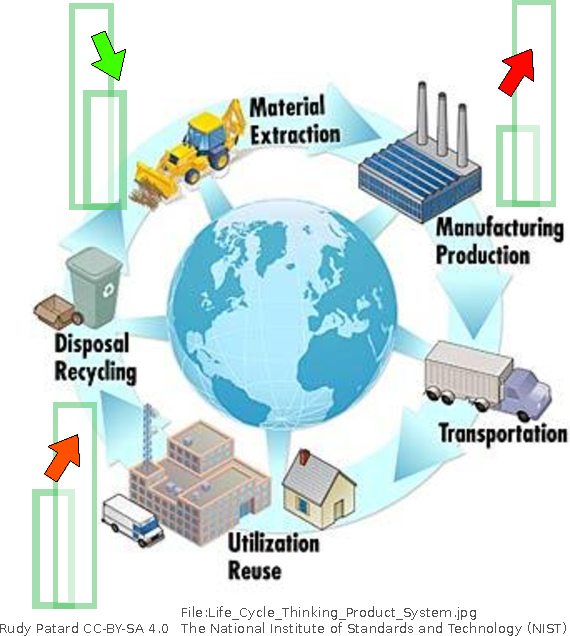
\includegraphics[width=0.5\textwidth]{/home/rudy/Documents/rudy/01_These/11_production/01_COMMUNICATION/02_PRESENTATION/BEAMER/images/report_impacts_phases_vie.pdf}
\caption{Illustration du report d'impacts entre phases de vie.}
\label{fig:report_impacts_phases_vie}
\end{figure}
\figbox{Sur la figure~\ref{fig:report_impacts_phases_vie}, une action de réduction d'un impact sur une phase de vie du produit (l'extraction de matières premières), génère une hausse des impacts sur deux autres phases (en fabrication et en utilisation).}
\exbox{
L'électrification d'une motorisation va affecter la phase d'utilisation.
Les émissions de combustion d'un moteur thermique se situent à la localisation du moteur alors que celles de la production d'électricité se trouvent sur les sites de production.
La nature des émissions pour la production et le traitement en fin de vie d'un moteur thermique, du réservoir associé et de son carburant seront différentes de celles de la fabrication d'un moteur électrique, de la batterie associée et de la source d'électricité.
}

Ceci nous conduit au second type de report, celui en \emph{nature d'impact}.
\begin{figure}[htbp]
\centering
\includegraphics[width=0.5\textwidth]{/home/rudy/Documents/rudy/01_These/11_production/01_COMMUNICATION/02_PRESENTATION/BEAMER/images/report_impacts.pdf}
\caption{report en nature d'impact.}
\label{fig:report_impacts}
\end{figure}
\figbox{Sur la représentation~\ref{fig:report_impacts} est illustré un transfert entre indicateurs sur les ressources et indicateurs sur la santé humaine.
Il s'agit simplement d'une illustration à visé pédagogique, le nombre de dimension étant bien supérieur.}
\exbox{
Les travaux sur les motorisations thermiques et la réduction des émissions de $CO_2$, de $NO_x$ et de particules sont intéressantes sur ce point.
Alors qu'une combustion \emph{complète} libère de la vapeur d'eau et du dioxyde de carbone, différents points de fonctionnement et divers carburants et mélanges avec comburant produisent une gamme variée d'émissions.
Il en résultent de nombreux compromis possibles entre l'émission de particules et de gaz générant du forçage radiatif.
}

La diversité des émissions et de leurs effets produit une autre caractéristique de l'ACV, l'agrégation des impacts.
\exbox{
Plusieurs substances différentes peuvent avoir un même effet.
Par exemple~: la vapeur d'eau, le dioxyde de carbone, le méthane, sont des \gls{GES}, au même titre que le perfluorobutane, le cis-perfluorodecalin, le dimethyl ether, l'hexafluoroethane, le perfluoropropane\ldots mais qui chacun auront une durée et une ampleur d'effet différent.
De même une même substance peut avoir plusieurs effets.
%\footnote{ Plus de détails sont disponibles dans la section d'analyse des méthodes d'impacts (\ref{sec:impactsmethods})}.
Le chloroforme est caractérisé dans l'ILCD2011 (méthode d'impacts européenne) pour son effet sur les impacts de changement climatique ; de toxicité humaine, canérigène et non-cancérigène ; de formation de particule ; de formation d'ozone photochimique ; d’écotoxicité aquatique en eau douce.
Nitric oxide, Nitrogen dioxide, Nitrogen oxides,
les oxydes d'azotes sont caractérisés (ILCD2011) pour la formation d'ozone photochimique, l'acidification et l'eutrophisation terrestre et marine.
%Le protoxyde d'azote. Dinitrogen monoxide, n'a qu'un facteur et porte sur le réchauffement climatique.
}
Ainsi plus qu'aux substances, c'est à leurs effets qu'a trait l'information produite par l'ACV
\footnote{L'inventaire collectera évidement les substances, mais cette activité relève de l'analyse de procédé plus que de l'analyse en cycle de vie, bien que la seconde (ACV) nécessite la première (analyse de procédé).}.
Cette structuration vers les effets a pris en ACV deux courants qui tendent à se rejoindre.
Les méthodes orientées impacts et les méthodes orientées dommages relèvent d'un degré d'agrégation variable qui cherche un équilibre entre maîtrise de l'incertitude et la capacité de faire sens pour le décideur. %(\textit{cf.} section \ref{sec:methodesdimpacts})
\begin{figure}[htbp]
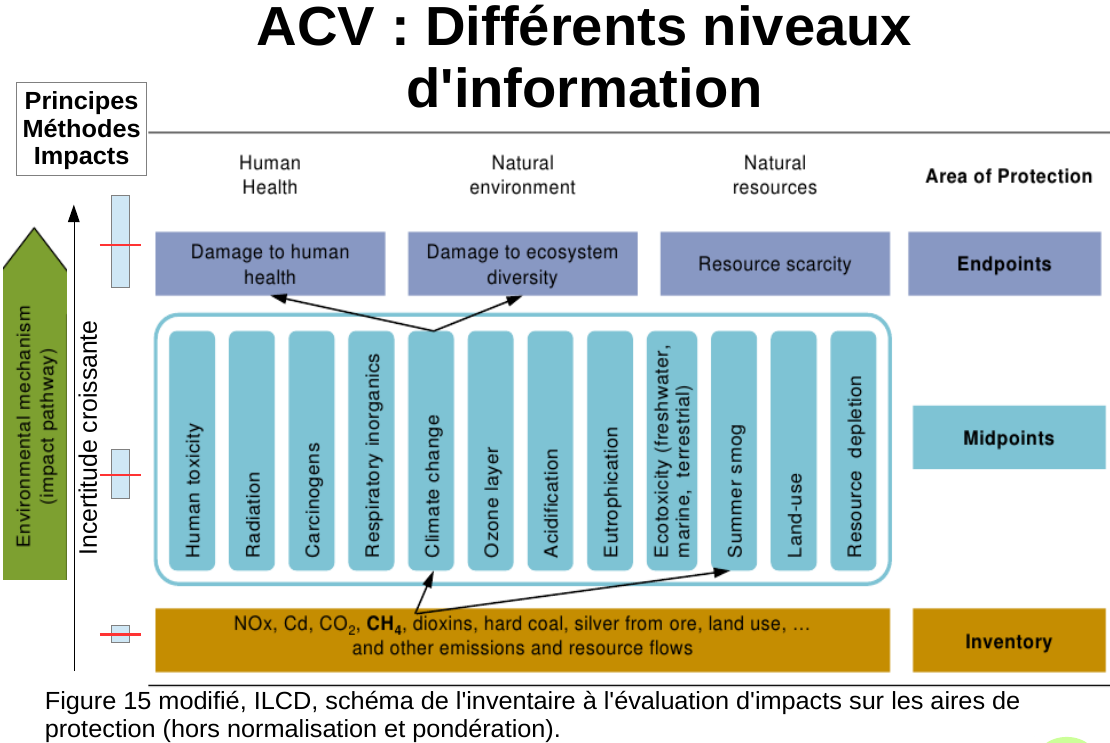
\includegraphics[width=\textwidth]{/home/rudy/Documents/rudy/01_These/11_production/01_COMMUNICATION/02_PRESENTATION/BEAMER/images/ILCD_principe_3_niveaux_information.png}
\caption{ILCD principe 3 niveaux information modified}
\label{fig:ILCD_principe_3_niveaux_information.png}
\end{figure}
\figbox{
La figure~\ref{fig:ILCD_principe_3_niveaux_information.png}, représente les agrégations midpoints et endpoints des indicateurs d'impacts en ACV.
La multiplicité des impacts par substance et la multiplicité des dommages par impacts est représentée par les flèches.
En ajout à la figure initiale nous avons représenté l'accroissement de l'incertitude au fil du déroulement des mécanismes environnementaux.}

Puisque l'ACV vise la sélection d'alternatives au sein de systèmes humains (décisions), il est tout à fait logique qu'elle se soit déployée avec l'intégration de dimensions sociales et économique, donc politiques.
%\colorbox{yellow}{ILCD stepwise extansion}
Ces caractéristiques combinées poussent la méthode dans une tendance holistique.
Puisqu'il n'est pas jugé a priori d'une importance supérieure d'un instant ou d'une nature d'impact, la méthode cherche à \emph{tout} circonscrire.
Puisque les activités humaines et éco-systémiques sont fortement et planétairement liées, l'aire d'étude porte rapidement sur tout le globe.

\subsubsection{Vocabulaire de base}
\label{subsubsec:Vocabulaire de base}
Nous nous contenterons de la description du vocabulaire tel qu'employé actuellement.
D'autres représentations sont possibles.
Une en sera donnée chapitre~\ref{chap:ACV, la (re)conception d'un outil}, plus particulièrement au point~\ref{par:Distanciation à la représentation classique de l'ACV}.
Nous nous attacherons dans cette présentation à identifier des origines historiques sur les termes afin de comprendre les racines méthodologique de l'\gls{ACV}.

\begin{figure}[htbp]
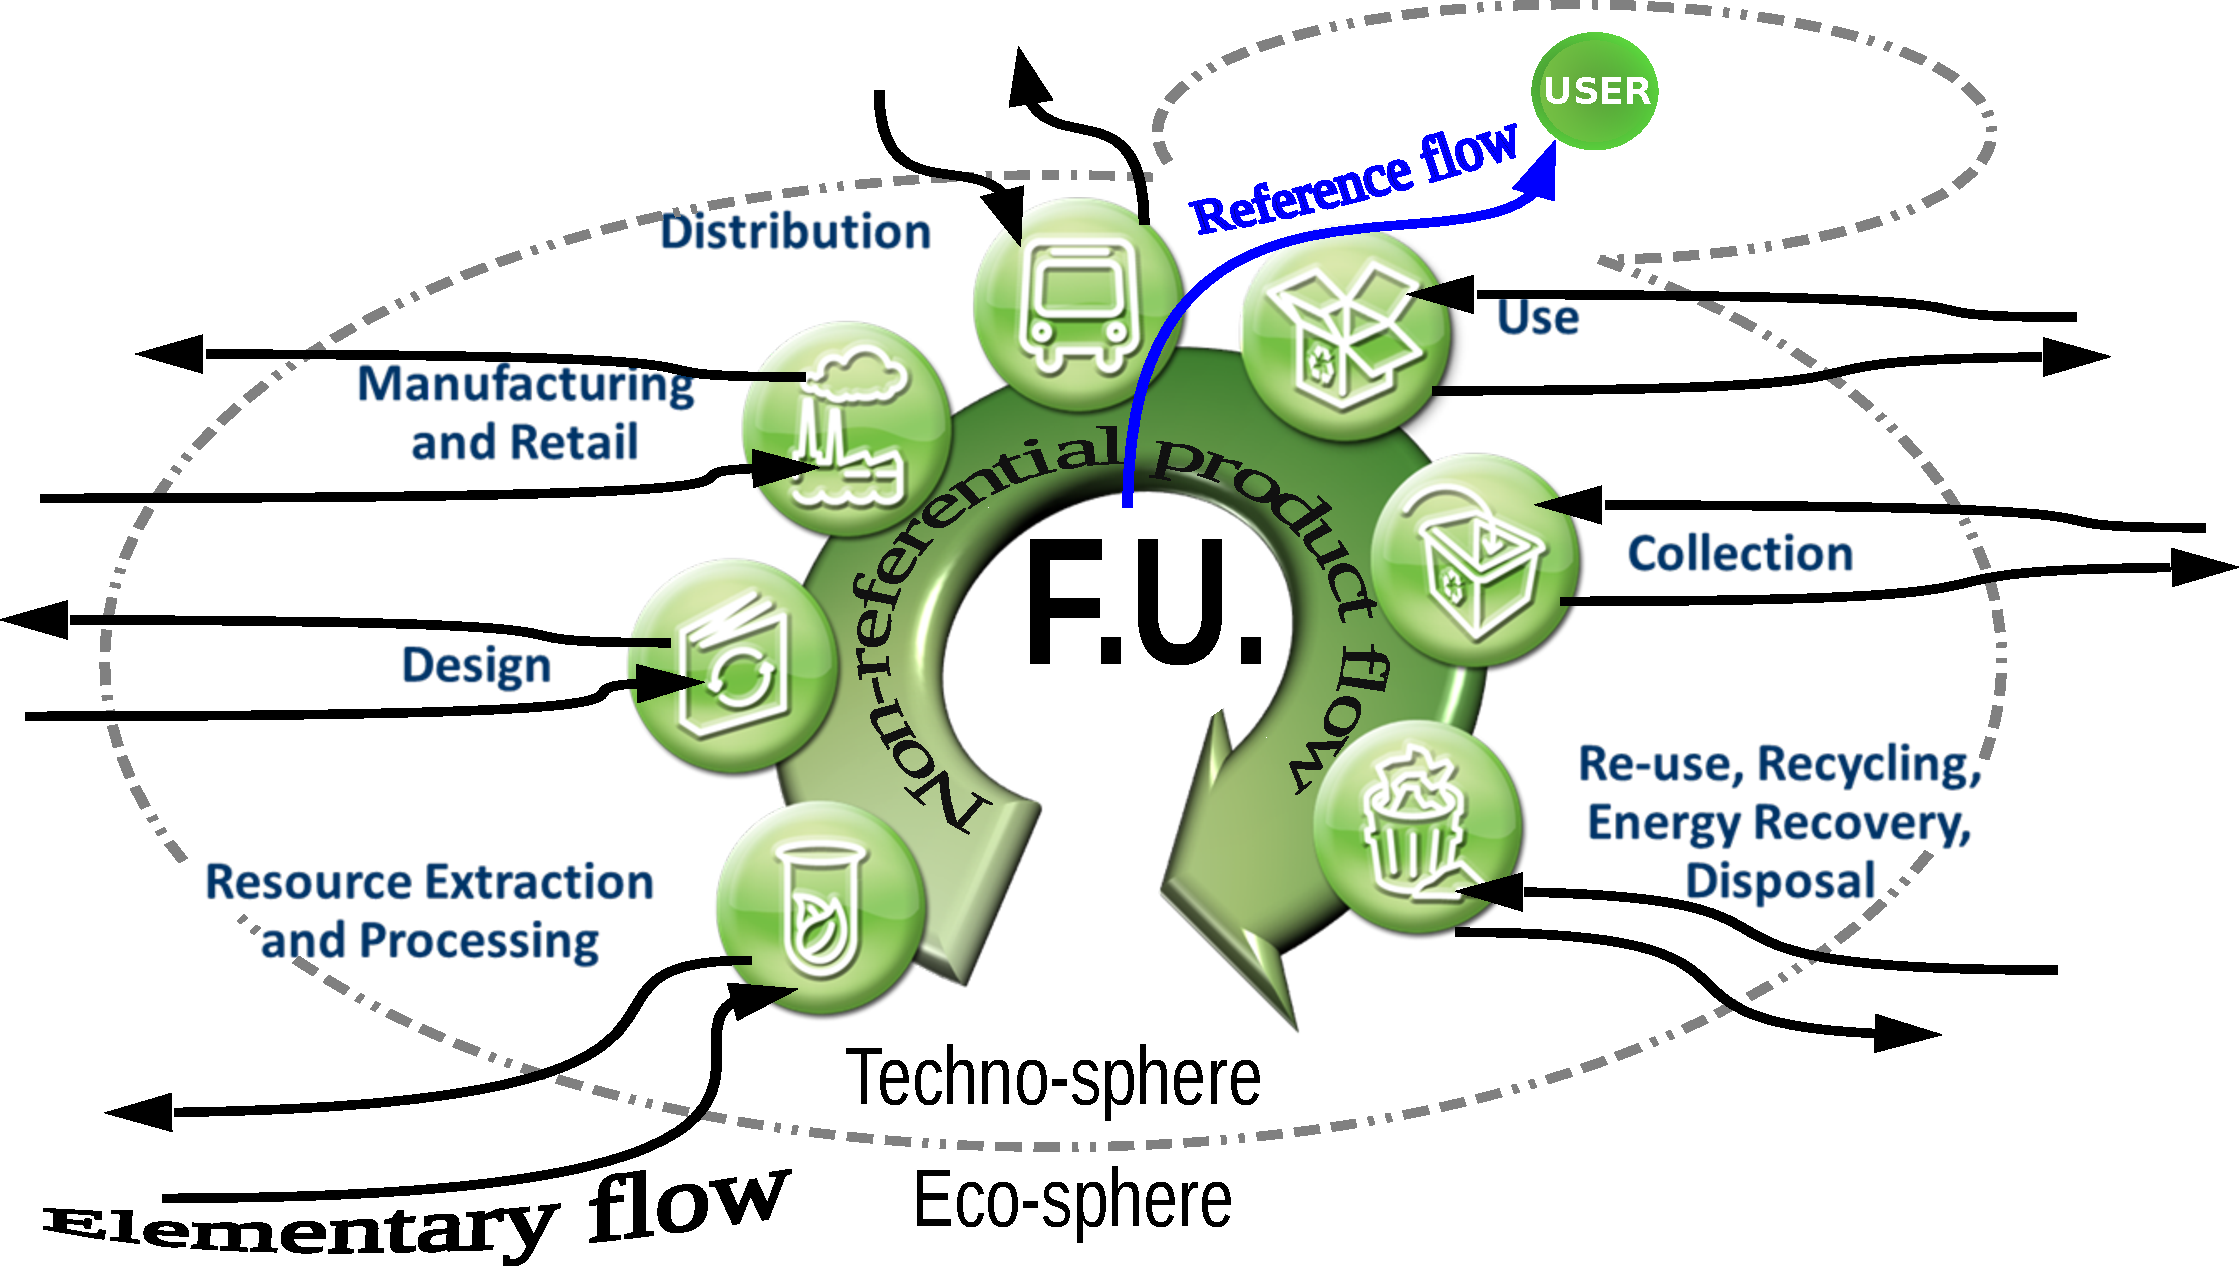
\includegraphics[width=\textwidth]{/home/rudy/Documents/rudy/01_These/11_production/01_COMMUNICATION/figures/cycle_ILCD_jrc_modif_EN.pdf}
\caption{Des flux qui comptent. Graphique Cycle ILCD modifié \cite{european_commission_ilcd_2010}.}
\label{fig:cycle_ILCD_jrc_modif}
\end{figure}
%\keybox{
\figbox{Dans la figure~\ref{fig:cycle_ILCD_jrc_modif}, nous posons un ensemble de mots clefs de la discipline.
Les \glspl{fluxelementaire} traversent la ligne pointillé démarquant \gls{technosphere} et \gls{ecosphere} (ou \gls{biosphere}).
Les \glspl{fluxproduit} s'échangent entre les étapes du cycle de vie, de 'l'extraction des ressources' à 'la fin de vie'.
Au centre de l'étude se trouve la clef de comparaison des alternatives, l'\gls{UF}.
Son unicité garanti la comparabilité des alternatives.
La délivrance de l'\gls{UF} à l'utilisateur est quantifiée par le \gls{fluxdereference}.
Chaque alternative comparée l'est sur la base de la même quantité du \gls{fluxdereference}.
L'ensemble des autres flux sont 'mis à l'échelle' pour conserver cette unicité de l'\gls{UF}.}
%}
\paragraph{La \gls{technosphere}} La recherche sur ce terme nous a conduit à des pistes interessante dans l'histoire de l'ACV. La \gls{technosphere} est le milieu des interactions humaines.
Absent du \citetitle{markandya_dictionary_2001}, l'\gls{ILCD} la définit au travers des flux élémentaires\footnote{\blockcquote[traduction]{european_commission_ilcd_2010}{
La frontière technosphère / écosphère peut donc être plus convenablement définie par la définition de flux élémentaire.
%The boundary technosphere / ecosphere can hence be more suitably be defined by defining the elementary flow.
}} (voir ci-après).
La complexité de sa définition n'est pas surprenante lorsque l'on observe sa formation par délimitation des voisins.
\blockcquote[traduction]{bruni_cognitive_2011}{Il est difficile de retracer l'origine exacte du terme "technosphère".
Il est clair cependant que le concept est un dérivé de ceux, complémentaires, de Eduard Suess et Vladimir Verdnasky de "bio-sphère" et de la notion de Teilhard de Chardin de "noosphère".}
%It is hard to trace back the original coining of the term “technosphere”. It is clear however that the concept is a derivative of Eduard Suess and Vladimir Verdnasky’s complimentary concept of “bio-sphere” and Teillard de Chardin’s notion of “noosphere”.
%}
%
Identifié par \citeauthor{bruni_cognitive_2011,} comme originaire de Michel \textsc{Batisse} (que nous n'avons pu vérifier), l'auteur la définit comme suit~:
\blockcquote[traduction]{bruni_cognitive_2011}{
Immédiatement au-dessus de la biosphère, et maintenant l'entourant entièrement, est un niveau plus élevé d'organisation, qui n'est devenu important que récemment, et qui peut être appelé la technosphère.
Elle est non seulement composée des usines, des barrages et des champs irrigués, mais aussi de tout le canevas des faits technologiques et des caractéristiques de natures physiques, chimiques ou biologiques (Batisse, 1973).}
%Immediately above the biosphere, and now surrounding it entirely, is a higher level of organization, which has become important only recently, and which can be called the technosphere. This is not only made up of the factories, the dams and the irrigated fields, but also the whole canvas of technological facts and features of a physical, chemical or biological nature (Batisse, 1973)
%}
De façon intéressante, dans cette représentation la techno-sphère se développe sur et autour de la biosphère ("surrounding it").
C'est une représentation opposée à celle de l'ACV, d'une technosphère \emph{entourée} d'\emph{éco}sphère.

Nous avons pu remonter dans l'histoire de ces termes jusqu'en 1968 (\citeauthor{milsum_technosphere_1968}, \citetitle{milsum_technosphere_1968}~\cite{milsum_technosphere_1968}).
Mais c'est en 1969 que l’occurrence la plus significative fut trouvée~\cite{iugg_i.u.g.g._1969}.
Parce que les termes employés sont significatif par leur similarité au langage de l'ACV actuelle, voici un extrait, sans traduction, du rapport.
\blockcquote{iugg_i.u.g.g._1969}{The ad hoc Committee has considered in detail the following ways in which man is altering the environment:\\
1. Increase in human population density.\\
2. Increase in \textbf{atmospheric carbon dioxide} from the combustion of fossil fuels.\\
3. Increase in turbidity (\textbf{particulate} content) of the atmosphere.\\
4. Pollution of the \textbf{oceans} and \textbf{coastal waters}.\\
5. \textbf{Radioactivity} in the atmosphere, natural waters, soils and living organisms.\\
6. \textbf{Deliberate and inadvertent modification of the atmosphere}, including the effects of cloud seeding and jet contrails.\\
7. Effects of introduced species.\\
8. Pressures on available \textbf{water resources}.\\
9. \textbf{Eutrophication} of international waters.\\
10. \textbf{Soil erosion and destruction}.\\
11. \textbf{Noise} as a pollutant.\\
12. Dissemination of \textbf{pollutants in air, soils, water} and living organisms (including Industrial and domestic \textbf{wastes}, pesticides, reactions In the atmosphere, biological molecules).\\
13. \textbf{Degradation of natural ecosystems with the loss of gene pools}.\\
14. Thermal pollution (atmosphere and international waters).
%There Is a wide variability in the scale of these effects, In the urgency of environmental threats, in the ways in which man could be affected.
%The Committee considered these facts, and also took note of the other International organizations which are Involved.
%The principal conclusion of the Committee Is that ICSU has a responsibility to provide objective scientific leadership In this field,
[\ldots] The ad hoc Committee recommends that ICSU set up a \textbf{Scientific Committee on Problems of the Environment} (SCOPE),
%[\ldots]
which would \textbf{bring together the various disciplines}, and which, through Its Commissions, would be responsible for the promotion of \textbf{environmental monitoring}, \textbf{evaluation of the effects of environmental disturbance} , \textbf{simulation modelling and predictions}, and the study of the \textbf{social effects} of man-made change in the environment.
%It Is recommended that SCOPE be provided with a secretariat which should be developed into as International Centre for the Environment.
%The ad hoc Committee recommends that SCOPE and the International Centre for the Environment cooperate fully with other groups, outside of ICSU, including all Involved UN Agencies, regional intergovernmental bodies, and international nonM-BM--governmental bodies.
[\ldots]
The commissions should in the first instance include:
(i) commission on monitoring,
\textbf{(ii) commission on biosphere and technosphere evaluation,}
(iii) commission on quantitative predictions,
(iv) commission on \textbf{social and economic evaluation}.}
%cat -v pour netoyer le fichier.
%clean with emacs ? C-M-s pas encore compris, but : ne garder que de l'ASCII
%http://tex.stackexchange.com/questions/4268/inputenc-error-unicode-char-u8-error-while-trying-to-write-a-degree-symbol#4270
Il semble peu probable que ces commissions se soient établies sans antériorités des termes et des recherches qui en composent les noms et activités.
Vous constaterez comme moi que la quasi totalité des termes courant de la pensée en cycle de vie s'y retrouve.
Pour autant nous n'y trouvons pas les mécanismes d'évaluation.
, même l'inclusion de la nuisance du bruit, toujours en discussion pour l'intégration aux méthodes d'impact aujourd'hui.

%\footnote{
%%Le \href{https://books.google.com/ngrams/graph?content=technosphere&year_start=1800&year_end=2000&corpus=15&smoothing=3&share=&direct_url=t1\%3B\%2Ctechnosphere\%3B\%2Cc0#t1\%3B\%2Ctechnosphere\%3B\%2Cc1}{NgramViewer de technosphere} (bien que revoyant à 1938) renvoi à Milsum, J. H. (1968) "Technosphere, Biosphere and Sociosphere", General Systems, 13. (il est plus probable que Milsum ait écrit en 68 qu'en 38).
%Des références à l'IUGG International Union of Geodesy and Geophysics et à l'ICSU International Council of Scientific Unions (1965 -66 -68 -69), référence sur lequelles nous n'avons pas pu mettre la main. Des requêtes ont été adressées à l'ICSU et l'IUGG.}


\paragraph{La \gls{biosphere} ou l'\gls{ecosphere}.}
Si la littérature semble plus employer la première que la seconde\footnote{\href{https://books.google.com/ngrams/graph?content=biosphere,ecosphere&year_start=1800&year_end=2008}{lien vers ngrams comparatif~: ecosphere, biosphere}} \footnote{\href{https://books.google.com/ngrams/info}{Lien vers les explications des ngrams}.}, l'ILCD se réfère à l'\emph{éco}-sphère.
Ce choix se comprends au travers des dimensions observées en ACV.
L'épuisement des ressources n'est pas du domaine du vivant.
Mais suivant les définitions employées de biosphère (voir plus bas), ce choix n'est pas sans contradiction.
L'\gls{ecosphere} n'est pas définie directement, mais comme la techno-sphère, sa définition résulte de celle du flux élémentaire.
Une représentation en est donnée \cite[figure 13 p.99]{european_commission_ilcd_2010}.
Elle y est périphérique à la techno-sphère.
La définition ACViste a ceci de particulier que dans son approche actuelle, l'écosphère, par complément de la techno-sphère, est l'espace où il n'y a pas d'intervention humaine, or ceci relève d'une inconsistance lorsqu'elle intègre l'homme dans sa 'matière vivante' avec les impacts attenants.

La double définition de biosphère du \citetitle{markandya_dictionary_2001}, présente celle-ci à la fois comme la région de la terre où la vie existe et les éléments constitutifs de la vie elle même (matière, énergie, information).

\paragraph{Le \gls{fluxelementaire}} est un concept clef pour les définitions en ACV. Un flux élémentaire est d'après l'ILCD une \blockcquote[traduction et synthèse d'un extrait de "Terms and concepts" p.94]{european_commission_ilcd_2010}{substance unique ou énergie extraite de, respectivement émise dans, l'\gls{ecosphere}, sans transformation humaine, précédente, respectivement suivante.}
%“single substance or energy entering the system being studied that has been drawn from the ecosphere without previous human transformation, or single substance or energy leaving the system being studied that is released into the ecosphere without subsequent human transformation”.
%material or energy entering the system being studied that has been drawn from the environment without previous human transformation, or material or energy leaving the system being studied that is released into the environment without subsequent human transformation”}
Puisque la définition de l'éco-sphère intervient dans la définition donnée par l'ILCD du flux élémentaire et réciproquement, la reformulation qui nous semble la plus pertinente est~:
Échange d'une substance qui, soit n'a jamais subi intentionnellement d’interaction humaine antérieure, soit n'en subit plus ultérieurement.

Ceci permet donc la définition itérative de la frontière techno-éco sphère sans l'appel de l'un des deux concepts et sans contradiction avec les impacts (interaction non-intentionnelle).
La notion primordiale est donc l'interaction humaine intentionnelle.
Les autres notions en sont des dérivations.
\paragraph{Le \gls{fluxproduit}} est définit par l'ILCD de la façon suivante~:
\blockcquote[traduction p.22]{european_commission_ilcd_2010}{
Un des flux de co-produits dans l'inventaire d'un procédé ou système qui accompli la fonction du procédé / du système.
Voir également~: Flux non-fonctionnel.
%One of the (co-)product flow(s) in the inventory of a process or system that fulfils the processus' / system's function. See also: Non-functional flow
}
\footnote{Inconsistance du référentiel méthodologique : \blockcquote[p.22]{european_commission_ilcd_2010}{Non-functional flow: Any of the inventory items that are not (co-)product flows. E.g. all emissions, waste, resources \textbf{but also} input flows of processed goods and of services.}
Le lecteur comprendra que si un flux est extrait de la biosphère pour \emph{servir} sous forme de biens et services, il recèle un caractère utile et \emph{fonctionnel}.}

\paragraph{Le \gls{fluxdereference}}, ou flux référentiel, ou encore reference flow pour les anglophones.\blockcquote[Traduit de Terms and concepts: Function, functional unit, and reference flow p.60]{european_commission_ilcd_2010}
{Le flux de référence, finalement, est le flux (ou les flux en cas de procédés multifonctionnels) auquel tous les autres flux entrant et sortant se rapportent. Il est celui qui réalise l'unité fonctionnel~: Le flux de référence peut être directement exprimé en relation à l'unité fonctionnelle.}
%
%The reference flow, finally, is the flow (or flows in case of multifunctional processes) to which all other input and output flows (i.e. all elementary flows and non-reference product and waste flows) quantitatively relate. It is realising the functional unit: The reference flow can be expressed in direct relation to the functional unit (e.g. “Complete coverage of 1 m 2 primed outdoor wall for 10 years at 99.9 \% opacity with paint A") or in a more product-oriented way (e.g. "0.67 l paint A").
%}

Pour plus de définition, nous renvoyons le lecteur à \citetitle[section 3 Key definitions]{european_commission_ilcd_2010} et aux encarts 'Terms and concepts'~\cite{european_commission_ilcd_2010}.

\subsubsection{L'Analyse du Cycle de Vie en détails}
L'analyse en cycle de vie comporte 4 étapes selon l'\gls{ISO}, 5 selon l'\gls{ILCD}.
\begin{figure}
\centering
\includegraphics[width=\textwidth]{/home/rudy/Documents/rudy/01_These/11_production/01_COMMUNICATION/figures_extraites/LCA-phase.pdf}
\caption{Cadre de travail et phase de l'ACV~\cite{european_commission_ilcd_2010}.}
\label{fig:LCA-phase}
\end{figure}
\figbox{Les flèches alternées de la Fig.~\ref{fig:LCA-phase} représentent le caractère itératif de la méthode.
Les applications de la méthodologies sont listés à droite des étapes qui sont~: la définition des buts, définition du périmètre, production et analyse de l'inventaire, caractérisation et interprétation.
%\exbox{test}
}
\paragraph{Itérative},
\blockcquote[]{european_commission_ilcd_2010}{
Dispositions~: 4 L'approche itérative pour l'ACV\\
I) Possible - Aperçu de l'approche itérative~: Il est recommandé de prendre une approche itérative pour l'étude ICV / ACV% (pour plus de détails voir le chapitre 2.2.4)
%Provisions: 4 The iterative approach to LCA
%I) MAY - Overview of iterative approach: It is recommended taking an iterative approach to the LCI/LCA study (for more detail see chapter 2.2.4)
\ldots
}
% nltk 'iterative' occurences ?
\paragraph{Définition du but de l'étude.}
Cette étape détermine la question de recherche, l'objectif à atteindre par sa résolution.
C'est cette réflexion qui détermine l'\gls{UF} ainsi que les alternatives qui seront étudiées.
Remarque~: L'expression du but peut précéder la réalisation d'une \gls{AF} des objets d'études.
Mais il est à prévoir qu'en l'absence d'\gls{AF} préliminaire, l'\gls{UF} sera révisée à son issue.
\paragraph{Définition du périmètre.}
Suivant la définition de l'\gls{UF}, un nombre variable de procédés seront nécessaires pour satisfaire sa délivrance.
Dans l'approche actuelle, le but de l'étude et les alternatives considérées peuvent modifier l'inclusion ou l'exclusion dans le périmètre.
Tout périmètre valide est celui qui ne modifie pas les conclusions de l'étude conformément à son but.
\exbox{Exemple d'exclusion de périmètre considéré comme praticable.
La confrontation pour le choix entre deux alternatives mettant en œuvre un système commun et ce dans les mêmes proportions permettra à l'analyste d'exclure du système étudié ces systèmes dont la comparaison (différence) est connue d'avance car nulle.
L'effet sur le résultat invite donc à l'exclusion.
Toutefois, le constat de l'équilibre permettant l'exclusion se fait à posteriori.
Sont intérêt est donc limité.}
\paragraph{Réalisation et analyse de l'inventaire.}
La réalisation de l'inventaire concerne la modélisation du système socio-technique délivrant l'\gls{UF}.
Le travail d'inventaire consiste en la collecte et le traitement des données d'observation du système étudié.
Partant des procédés identifiés au périmètre initial (satisfaisant la délivrance de l'\gls{UF}), il s'agit de renseigner l'ensemble des flux, produits et élémentaires, entre l'ensemble des procédés dans la \gls{technosphere} ainsi qu'entre ces procédés et la \gls{biosphere} sous ses diverses compartimentations.
Son résultat est l'\gls{ICV}.
L'étape cristallise les problématiques de multifonctionnalité et de disponibilité des données, traitées respectivement au \ref{chap:Multifonctionnalité} et au \ref{chap:Recherche Libre}).
Dans sa conception actuelle, cette étape est concentrée sur les données de la \gls{technosphere}.
La modélisation des systèmes environnementaux étant réduite à l'utilisation de méthodes d'impacts, nous la traitons dans l'étape suivante.

\paragraph{Évaluation des impacts.}
Cette étape est également dénommée caractérisation.
Sur la base de l'ensemble des flux élémentaires collectés et affectés à leurs compartiment respectifs (air, eau, sol et sous-catégorisations), les effets sur les mécanismes environnementaux sont évalués à diverses échelles (tel que représenté Fig~\ref{fig:ILCD_principe_3_niveaux_information.png}).
Les méthodes d'impacts sont observées section~\ref{sec:LCIAM}
Il résulte de cette étape une liste d'indicateurs caractérisés.
\paragraph{Interprétation.}
Souvent détaillée pour l'interprétation finale, il est à noté qu'en figure~\ref{fig:LCA-phase} elle apparaît bien à chacune des étapes.
Avant le traitement de de la caractérisation, l'interprétation vise donc à contrôler l'ensemble des étapes précédentes à chaque pas (le périmètre respectivement au but, l'inventaire respectivement au but et au périmètre etc.).

Le cœur de l'étape d'interprétation consiste en la réduction des données sous une forme exploitable pour la décision.
Le regroupement en aires de protection (indicateurs de dommages) ou en score unique font partie de ce traitement.
Les opérations actuellement détaillées dans la méthodologie portent sur la pondération et la normalisation.

%Il s'agit ci-après des pondérations réalisées dans le cadre d'études liées à l'environnement.
%Une synthèse de la classification de \citeauthor{rowley_aggregating_2012} reprenant \textsc{Finnveden}, 1999
%%~\cite{finnveden_critical_1999}~;
!!!PB ref finnveden critical 1999 : Missing number, treated as zero.

 \textsc{Lindeijer}, 1996~; \textsc{Hofstetter}, 1996 et \textsc{Powell}(1997)~\cite{powell_approaches_1997} a été faite.
L'interprétation se fait donc~:
\begin{itemize}
\item Par sélection (équipondérée). (monocritère ou en nombre réduit les autres étant négligés)
\item Par monétarisation~:
%\footnote{avec ici la distinction faite par \citeauthor{powell_approaches_1997} entre coût du contrôle environnemental et coût du dommage environnemental.}
\begin{itemize}
\item Par coût du contrôle environnemental. 
Le poids est attribué suivant le coût représenté par les mesures de contrôle d'émission de la substance.
\item Par coût du dommage environnemental.
Le poids est attribué suivant l'\emph{estimation} du coût engendré par les dommages liés à l'émission de la substance.
Par exemple, la méthode basée sur la ``volonté à payer'' des individus pour la protection ou la réparation.%
%\footnote{HARRIBEY dans\cite{harribey_richesse_2013} précise que les valeurs monétaires estimées l...
\end{itemize}
\item Par Distance à la cible. Les cibles peuvent être dérivées de réglementations ou de limites jugées utiles pars un corps tiers et estimées scientifiquement~\cite{seppala_meaning_2001}.
\item Par panel. Les travaux de \citeauthor{myllyviita_impact_2014} portent sur l'étude de la pondération par panel. (Où : Comment un groupe de personnes attribue des poids aux indicateurs~?)~\cite{myllyviita_impact_2014}.
\end{itemize}

Ces opérations sont critiquées section~\ref{chap:Jugements et Multi-dimensionnalité}.
Cette étape est évidement centrale dans notre travail d'intégration du jugement dans la méthodologie.


\subsubsection{Synthèse des caractéristiques méthodologiques spécifiques}
{Itérative} et {Multi-critère} dans sa quête holistique, l'\gls{ACV} se déploie par étapes pour
(i) fixer ses objectifs et son cadre décisionnel,
(ii) établir sa clef de comparaison qu'est l'\gls{UF},
(iii) comptabiliser ses échanges de \glspl{fluxproduit} dans la \gls{technosphere} et de \glspl{fluxelementaire} avec la \gls{biosphere},
(iv) puis évaluer les effets sur les mécanismes environnementaux en caractérisant des indicateurs d'impacts,
(v) et enfin faire l’interprétation de cette caractérisation.

Nous venons donc de voir les caractéristiques actuelles et les fondements de l'\gls{ACV}.
Observons maintenant leurs causes et origines.

\subsection{L'origine de l'ACV}
\label{subsec:L'origine de l'ACV}

Nous avons cherché l'origine de l'évaluation en cycle de vie dans le premier numéro du journal international éponyme.
\citeauthor{hunt_lca-_1996} dans \citetitle{hunt_lca-_1996}, attribuent l'origine de l'ACV au travail de
\blockcquote{hunt_lca-_1996}{Harry E. TEASLEY, Jr.} en 1969, travaillant pour la célèbre marque de boisson pétillante caféinée.

\citeauthor{boustead_lca_1996} dans \citetitle{boustead_lca_1996}, situe également les premiers pas de ce qui deviendra l'ACV par l'évaluation des matériaux d'emballage et notamment le packaging en verre des boissons avec la méthode d'énergie cumulée.
Cette introduction est fort intéressante en ce qu'elle dévoile la mixité et proximité des activités économiques, académiques et politiques.

\citeauthor{boustead_lca_1996} nous offre en effet un tableau comprenant~:
\begin{itemize}
\item Des groupes de pression (Amis de la Terre) s'opposant aux groupes industriels~\footnote{
\blockcquote[traduction]{boustead_lca_1996}{
Les Amis de la Terre ont renforcé leur position par le déversement d'un camion chargé de bouteilles vides non récupérables sur le seuil du siège social de Schweppes à Londres.
%Friends of the Earth reinforced their stance by dumping a truck-load of empty non-returnable bottles on the doorstep of Schweppes head office in London
}
},
\item Des groupes des industriels cherchant défenses et cautions scientifiques~:
%\footnote{
\blockcquote[traduction]{boustead_lca_1996}{
La fédération des producteurs de verre a décidé qu'ils avaient intérêt à obtenir des informations quantitatives définitives avec lesquelles monter leur défense.
%the Glass Manufacturers Federation decided that they had better get some definitive quantitative information with which to mount their defence.
}
%},
\item La Recherche leur fournissant `expertise et caution' scientifique contre du financement~:
%\footnote{
\blockcquote[traduction]{boustead_lca_1996}{
L'\textit{Open University} était une institution nouvelle et avait peu de fonds pour la recherche.
Donc, l'exécution des travaux de sous-traitance fournirait des fonds pour notre recherche universitaire.
%the Open University was a new institution and had few research funds. So carrying out contract work would provide funds for our academic research.
}
%},
\item L'inter-relation au contexte international et aux crises politico-économiques (73 notamment)~:
%\footnote{
\blockcquote[traduction]{boustead_lca_1996}{
Il s'était donc trouvé que lorsque la première crise du pétrole frappa, nous poursuivions une double approche à l'analyse de l'énergie.
%So it was that when the first oil crisis hit, we were pursuing a twin-track approach to energy analysis.
}
\footnote{Ladite crise de 1973, se situe entre 71 et 73 selon que l'on considère le pic de production américain, la modification des propriétés de conversion du dollar, ou l'embargo de l'OPEP.}
%}.
Les lecteurs attentifs ou les experts du domaine n'auront pas raté la proximité chronologique du rapport \citetitle{meadows_limits_1972}.
\item Le contraste du rapport aux données selon les intérêts gouvernementaux entre économistes et écologistes~:
%\footnote{
\blockcquote[traduction]{boustead_lca_1996}{
Dans les premiers jours un problème majeur était le manque de données primaires fiable d'origine industrielles et nous avions l'habitude de regarder avec envie nos cousins économistes qui ont accès aux vastes exercices de suivi effectués aux frais du gouvernement.
%In the early days one major problem was the shortage of reliable industry based, primary data and we used to look with envy at our economist cousins who had access to the vast monitoring exercises carried out at government expense.
}
%}.
\end{itemize}
Un trait intéressant de ces retours historiques est d'observer l'omniprésence dans un espace de `recherche', d'organismes dépendant de contrat avec des parties prenantes à caractère industriel, commercial et lucratif.
Un état de fait qui a perduré jusqu'ici.

C'est toutefois dehors de cette parution nous trouvons des éléments de similarité à l'ACV des plus intéressants.
Si intéressants que nous n'y voyons rien d'autre que les origines de l'ACV.
Nous avons déjà vu dans la section sur le vocabulaire l’extrême similitude quant au SCOPE et ses commissions (en 69) (\ref{subsubsec:Vocabulaire de base}).
En \citeyear{leontief_environmental_1970}, dans son article \citetitle{leontief_environmental_1970},  \citeauthor{leontief_environmental_1970} décrit une approche par "entrée-sorties" dont le vocabulaire ne manquera pas non plus de similitude à l'ACV.

\blockcquote[traduction]{leontief_environmental_1970}{
La pollution est un co-produit des activités économiques habituelles\footnote{Vous noterez bien, la polution est une co-production (original~: POLLUTION is a by-product)}.
Dans chacune de ses multiples formes, elle est reliée de façon mesurable à une consommation particulière ou un procédé de production.
La quantité de monoxyde de carbone relâchée dans l'air porte, par exemple, une relation définie à la quantité de carburant brûlée par divers types de moteurs d'automobiles ; le rejet d'eau polluée dans les courants et les lacs est directement lié au niveau de production d'acier, de papier, de textile et de toutes les autres industries utilisant l'eau et sa quantité dépend, dans chaque cas, des caractéristiques technologiques de l'industrie particulière.
[\ldots]
Dans ses versions plus compliquées multi-régionale et dynamique l'approche entrées-sorties nous permet d'expliquer la distribution spatiale des productions et consommations de biens et services variés.
[\ldots]
Fréquemment non-remarqués et trop souvent négligés, des co-produits indésirables (autant que certaines entrés d'origine naturelle, précieuses mais non-payées) sont liés directement au réseau de relations physiques qui gouvernent jour après jour les opérations de notre système économique.
%POLLUTION is a by-product of regular economic activities.
%In each of its many forms it is related in a measurable way to some particular consumption or production process:
%The quantity of carbon monoxide released in the air bears, for example, a definite relation-ship to the amount of fuel burned by various types of automotive engines;
%the discharge of polluted water into our streams and lakes is linked directly to the level of output of the steel, the paper, the textile and all the other water-using industries and its amount depends, in each instance, on the technological characteristics of the particular industry.
%[\ldots]
%In its more complicated multi-regional and dynamic versions the input-output approach permits us to explain the spatial distribution of output and consumption of various goods and services.
%[\ldots]
%Frequently unnoticed and too often disregarded, undesirable by-products (as well as certain valuable, but unpaid-for natural inputs) are linked directly to the network of physical relationships that govern the day-to-day operations of our economic system.
}

S'ajoute à cela l'articulation mathématique actuelle de l'ACV que nous extrayons sans traduction de l'ouvrage de \citeauthor{heijungs_computational_2002} intitulé \citetitle{heijungs_computational_2002}, présentée dans le tableau~\ref{tab:heijungs_computational_2002}.
\begin{table}[htbp]
\centering
\begin{tabular}{p{3.5cm} | p{2cm} | p{3.3cm} | p{3cm}}
life cycle inventory analysis & LCA & input-output analysis & lOA \\
\hline
product, economic flow & & commodity &  \\
(unit) process & & industry, sector, establishment transactions matrix & $z$ \\
technology matrix & $A$ & technical coefficients matrix & $\tilde{Z}$ \\
final demand vector & $f$ & households demand vector & $y$ \\
scaling vector & $s$ & total output vector & $x$ \\
inverse of technology matrix & $A^{-1}$ & Leontief inverse & $(I-\tilde{Z})^{-1}$ \\
intervention matrix & $B$ & satellite matrix & $\tilde{B}$ \\
equation for s & $s = A^{-1} f$ & equation for x & $x = (I - \tilde{Z})^{-1} y$ \\
equation for g & $g=Bs$ & equation for g & $g=\tilde{B}x$ \\
\end{tabular}
\caption{\cite[Table 5.1: Overview of analogous concepts in life cycle inventory analysis and input-output analysis.]{heijungs_computational_2002}}
\label{tab:heijungs_computational_2002}
\end{table}
\figbox{
\citeauthor{heijungs_computational_2002} déclarent à l'occasion de cette table (\ref{tab:heijungs_computational_2002}) qu'il y a de subtiles différences entre les formalismes~: une approche IOA `industrie par industrie' (ou secteur par secteur) et une approche LCA commodités par procédé et un certain nombre de conséquences associées.
Nous soulignons \emph{toutefois} que la problématique de la multi-fonctionnalité (plusieurs commodités par procédés) n'a pas encore été unanimement résolue.
Il parait donc inapproprié de dire que nous sommes émancipés de l'œuvre et donc des principes de \citeauthor{leontief_environmental_1970}.
}

Il ne nous en faut pas plus pour caractériser l'origine de ce qui passera d'éco-profil (resource and environmental profile analysis, REPA) à l'ACV
\footnote{
\blockcquote[traduction]{hunt_lca-_1996}{
Le terme historique pour ces études de cycle de vie de l'environnement était Ressource et d'Analyse de Profil Environnemental (REPA), un terme qui a été utilisé depuis 1970.
%The historical term for these environmental life cycle studies was resource and environmental profile analysis (REPA), a term that has been used since 1970.
}
}.
%O’Brien, M.; Doig, A.; Clift, R. Social and environmental life cycle assessment (SELCA). Int. J. Life Cycle Ass. 1996, 1, 231–237.
%\cite{heijungs_computational_2002}

Ce qui peut-être cause la \emph{crise} de l'\gls{ACV}, c'est que le support de cette outil n'est plus à jour.
Le type de calcul selon \citeauthor{leontief_environmental_1970} avec inversion matricielle et coefficients constant est encore celui appliqué.

Les évolutions qui ont suivi n'ont pas encore été intégrées.
Mais l'intégration semble imminente.
C'est ce que nous voyons dans la section suivante.

\subsection{Historique, contexte et développement de la méthode}
\label{subsec:Historique de la méthode, son développement, son contexte}
Deux travaux définissent assez bien le développement de l'ACV et son état actuel, l'analyse bibliométrique de \textsc{Chen} et la revue de \textsc{Reap}.
Pour observer l'évolution de la discipline, nous employons tout d'abord les travaux de \citeauthor{chen_bibliometric_2014}~\cite{chen_bibliometric_2014}
\footnote{
Un travail similaire a été réalisé en \citedate{hou_mapping_2015} par \citeauthor{hou_mapping_2015}~\cite{hou_mapping_2015}. Le seul apport notable que nous en conservons et la confirmation que le sujet principale de la méthodologie passe après les applications ou un indicateur phare (Énergie ; GES - PRG).
}
\footnote{
Dans les travaux relatant la croissance des publications, nous n'avons pas observé de traitement particulier pour la croissance globale de la publication scientifique et relativiser les écarts entre période sur l'intensité de l'activité.
L'observation des travaux sur les 'REPA' masquent peut-être les travaux de la période 70-90.
}.


%\colorbox{red}{pb de (c) produire une figure nœuve sans le graphisme de \citeauthor{chen_bibliometric_2014}}
\begin{figure}[htbp]
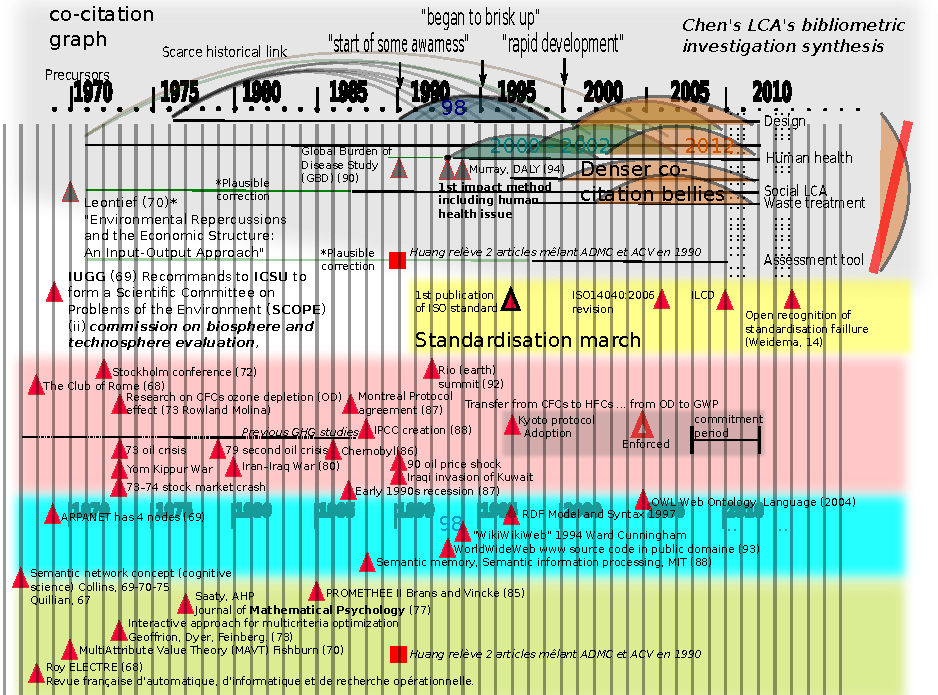
\includegraphics[width=1\textwidth]{/home/rudy/Documents/rudy/01_These/11_production/01_COMMUNICATION/figures/Chen_2014_bibliometric_chrono_modified.pdf}
\caption{Ligne chronologique de \textsc{Chen} et ses 26 clusters, (fig. 4 schematisée) et compléments du contexte académique et politique.}
\label{fig:bilbiometry_chrono_CHEN}
\end{figure}
\figbox{
Nous reprenons de façon schématique la représentation graphique de l'article de \citeauthor{chen_bibliometric_2014}~\cite{chen_bibliometric_2014} Fig.~\ref{fig:bilbiometry_chrono_CHEN}\footnote{\textbf{Zoomez sur le pdf tant que vous voudrez, l'image est vectorielle}.}.
Nous la complétons des éléments de contextualisation académique, technologique et politique que nous exploiterons dans diverses parties de ce mémoire.

Nous pouvons voir au travers du graphique de co-citation de \citeauthor{chen_bibliometric_2014} (i) des précurseurs dans les années 70 (ii) une période de vingt ans avec peu d'activité. Dans celle-ci, il est plus courant non pas de parler d'\gls{ACV} mais de REPA (resource and environment profile analysis)\cite{hunt_lca-_1996}.
(iii) Puis dans les années 90, une croissance rapide par groupe d'application apparaît avec des 'ventres' de citations plus denses.
Alors que le démarrage a pour occurrence la période de 70 un nouveau point de convergence et d'activité dans la décennie 90 est observé.

Nous soulignons sur cette figure stylisée la stratification par domaines d'application.
Nous ajoutons également sous le graphique initial~: le développement en informatique du web sémantique, avec notamment le modèle \gls{RDF} ; le développement de wikiwikiweb ; le développement des \gls{ADMC} ; ainsi que les conflits liés à l'énergie, notamment les chocs pétroliers.
Des rassemblements internationaux sur la question environnementale sont représentés, notamment ceux en lien avec des accords internationaux.

Vous remarquerez sur la question du \emph{protocole de Montréal}, considéré comme un \emph{succès} pour un accord international (premiers traités universellement ratifiés dans l'histoire des nations unis)\cite{unep_press_2012}, la résurgence de la question des \emph{rebonds en nature} (report des \gls{CFC} impliqués dans \gls{ODP}, vers les \gls{HCF} acteurs dans \gls{GWP}).
Ceci est mis en parallèle de \textit{l'échec} relatif sur le changement climatique et des substances tel le CO2\footnote{La discussion \href{http://www.nytimes.com/2016/07/24/world/europe/vienna-sequel-paris-climate-accord.html?_r=0}{d'accords parallèles} à ceux de Paris et la COP21 a ceci d'intéressant qu'elle souligne l'activité des lobbies lorsqu'une partie-prenante dominante (Honeywell ici) développe et défend en exploitation une substance alternative.
C'est à dire lorsqu'un acteur économique dominant a la capacité de maintenir ses avantages concurrentiels et son marché.}.

S'agissait-il du contexte international (Rio, chocs pétroliers, Chernobyl)
ou de la première méthode d'impacts avec indicateurs de santé humaine,
ou des progrès en informatique,
ou des premières intégrations de la décision multi-critère,
ou d'une combinaison de tout cela à la fois ?
%Is it due to the international context (Rome, Rio),
%or the first impact method using human health,
%or progress in informatics ...
%or some combination of all?
Toujours est-il que la standardisation de la méthode en cycle de vie a pris pied dans cette période de 90, en atteste la première publication relative à la norme ISO~\cite[ISO - Technical committees - ISO/TC 207/SC 5 - Life cycle assessment.]{iso_iso_1993} en 1993, la première 14040 sortant en 97.%ISO - Technical committees - ISO/TC 207/SC 5 - Life cycle assessment.
%Anyway the standardization took foot on this period of the nineties, as attest the first publication date of the corresponding standard\cite[ISO - Technical committees - ISO/TC 207/SC 5 - Life cycle assessment.]{_iso_????} 1993.%ISO - Technical committees - ISO/TC 207/SC 5 - Life cycle assessment.

Nous observons que les précurseurs de l'ACV et des outils que nous lui associons naissent à la même période.
Celui de l'internet (arpanet 69) s'accompagne de l'incroyable développement technologique des communications et des principes de l'open-source~\cite{raymond_cathedral_2001}.
Le même rebond en 90 voit la naissance d'internet et la libération de ses protocoles.
C'est également une période riche concernant les techniques de décision multi-critère (\citeauthor{roy_classement_1968} \textsc{Fishburn}).

Finalement, nous pouvons dire que \textbf{sur la période de 90, l'ensemble des outils conceptuels comme applicatifs sont donc réunis}.
Ils n'interagissent toutefois pas encore.
}

Voilà donc pour son historique et son contexte, qu'en est-il de l'état actuel ?
%So this was history.
%What about now?

Tout d'abord, rappelons que la recherche est faite par des personnes en relations, confrontant leurs idées sur un sujet.
Or, bien que la production d'ACV soit traitée numériquement, la communauté de l'ACV est un groupe déconnecté (pour reprendre les termes de \citeauthor{davis_industrial_2010} une \blockcquote{davis_industrial_2010}{offline community}).
Et bien que traitant de systèmes intrinsèquement complexes, nécessitant la jonction de multiples disciplines, nous ne sommes pas très efficaces pour joindre les pièces du puzzle~\cite{davis_industrial_2010}~\footnote{\blockcquote{davis_industrial_2010}{not so efficient at bringing these pieces together}}.
Ceci conforte l'analyse du réseau de co-citations de \citeauthor{chen_bibliometric_2014}, avec des citations transversales aux applications réduites.
%Apart from this state seen from two publications, what I would also consider is the connection state of LCA's community. We are basically an ``offline community''~\cite{davis_industrial_2010}.
%LCA's community in Davis's work is depicted to be unconnected\cite[1.1 Motivation]{davis_making_2012} and ``not so efficient at bringing these pieces together'' speaking of the different disciplines we interact with.
%This comfort the co-citation patterns from Chen, with clearly more limited cross application citation.
\blockcquote[traduction]{chen_bibliometric_2014}{
Donc, en tant que mesure de la structure du réseau, la mesure de la modularité du réseau générée est de 0,8282, ce qui suggère des connexions inter-clusters denses entre les nœuds, mais \emph{des connexions clairsemées entre des nœuds dans différents clusters}
%So as a measure of network structure, the modularity measure of the network generated is 0.8282, suggesting dense intercluster connections between the nodes but \emph{sparse connections between nodes in different clusters}
}.
%CHECK documentation latex chap 6 
% \usepackage{csquotes}
% \usepackage[backend=biber]{biblatex}
% \addbibresource{MaBiblio.bib}
% \SetCiteCommand{\autocite}
En fait, n'est-ce pas parce que nous sommes capable de trouver statistiquement des agrégats par domaines d'application que nous pouvons statuer sur la fragmentation applicative de notre domaine d'étude~\barre{?}.
Lorsque nous observons le cycle de vie d'un système, n'y a-t-il pas plus de procédés dans les diverses applications environnantes, dans l'arrière plan, que dans celui concerné par le "premier plan"~\barre{?}.
%In fact, isn't it because we can find statically clustered domains of applications that we can state that our discipline is fragmented by application fields?
%When we look at a system's life cycle, isn't there many more processes in different fields than the one concerned by the product or service we're looking at?
Ce constat est également visible par les remarques éditoriales telles celles de \citeauthor{klopffer_how_2014} dans \citetitle{klopffer_how_2014}~\cite{klopffer_how_2014}.
Il y a glissement entre ACV et analyses de procédés, qui donne une forte orientation applicative à la discipline.

Ce qui nous amène aux choses que les applications ne travaillent pas à résoudre, voir peut-être, ce dont elles freinent la résolution due à un mécanisme d'auto-renforcement (accroissement du coût à la renonciation et à la reconnaissance de l'erreur), \textbf{les problèmes méthodologiques de l'ACV}.
\subsection{Problèmes méthodologiques et conceptuels}
\label{subsec:Problèmes méthodologiques}
\citeauthor{klopffer_background_2014}, dans son ouvrage \citetitle{klopffer_background_2014}~\cite{klopffer_background_2014}, traite des revues de \citeauthor{reap_survey_2008} (\citetitle{reap_survey_2008})~\cite{reap_survey_2008}, \citeauthor{finnveden_recent_2009} (\citetitle{finnveden_recent_2009})~\cite{finnveden_recent_2009}\footnote{Sa revue germanophone avec \textsc{Grahl} nous est linguistiquement non-accessible.}
et d'une plus précoce (93) de \citeauthor{udo_de_haes_applications_1993}~\cite{udo_de_haes_applications_1993}.

Nous pouvons en effet nous demander ce qui a été résolu depuis la revue de \citeauthor{udo_de_haes_applications_1993} en \citeyear{udo_de_haes_applications_1993}~\cite{udo_de_haes_applications_1993}.
\citeauthor{udo_de_haes_applications_1993} pointait les éléments suivants.

\blockcquote[traduction]{udo_de_haes_applications_1993}{
%Survey of drawbacks and possible solutions
Un certain nombre d'inconvénients ont été mentionnés en ce qui concerne l'applicabilité de l'ACV, et en particulier l'ACV quantitative, comme un système d'aide à la décision.}\ldots
%A number of drawbacks have been mentioned with respect to the applicability of LCA, and in particular quantitative LCA, as a decision-support system. More specifically, 
\blockcquote[traduction]{udo_de_haes_applications_1993}{
Trois types de problèmes peuvent être identifiés~:
des problèmes purement techniques, des problèmes méthodologiques et des problèmes de communication.
%three types of problems can be identified:
%purely technical problems, methodological problems
%and communication problems.
}

\blockcquote[traduction]{udo_de_haes_applications_1993}{
Les problèmes purement techniques peuvent être décrites par "l'ACV est trop complexe, il n'y a pas assez de données, toute la procédure est trop longue et donc trop coûteuse".}
%The purely technical problems can be characterized as ' L C A is too complex, there are not enough data, the whole procedure is too time consuming and therefore too costly'.
%A solution can be sought in the development of databases and software.
%It has already been mentioned that a complicated method can be very easy to apply if user-friendly software is present.
%A further relief will take place with the development of databases. In view of the credibility of the results, both should be public. Up to now consultancy firms have regarded their software as a business secret. As long as LCA was not subject to public debate this worked well. At present it is highly advisable that, in line with the SETAC Code of Practice, public software be developed, including options for sensitivity analysis for the critical points of choice in the methodology and data variability.
%With respect to the databases, the development of one encompassing database for environmental inputs and outputs of all relevant processes seems unrealistic at present.
%One database per economic sector or branch may be more attainable.
%The recently published database of the Plastics Waste Management Institute (PWMI) in Brussels is at present the most well known example 28.
%Disadvantages of such a decentralized option can be limited if a general format of data storage can be adopted.
%For reasons of secrecy, companies may demand that the data are stored in an averaged form, which may limit their applicability.
%This problem is aggravated if data are presented not on single processes but on cradle-to-gate life cycles of materials as a whole, including choices on inventory methodology (see below).

\blockcquote[traduction]{udo_de_haes_applications_1993}{
Les problèmes méthodologiques concernent les différences entre les méthodes par rapport à des points importants de choix, l'incomplétude des méthodes, ou les deux.
Différents choix sont, par exemple, en jeu par rapport aux règles d'allocation dans l'analyse de l'inventaire.
La discussion sur les méthodes d'évaluation d'impact concerne à la fois l'incomplétude des méthodes (manque de connaissances sur les facteurs d'équivalence) et les différences d'opinions [\ldots à]
%ou même des écoles différentes (par exemple par rapport à la question de 
savoir si l'évaluation de l'impact doit être de préférence spécifique au site ou non-spécifique au site
%)
.}
%Poursuite de l'harmonisation, ou même la normalisation, est nécessaire, le long des lignes du code de bonnes pratiques déjà mentionnés.
%Cela devrait empêcher le développement de différentes écoles de méthodologie de l'ACV et finalement conduire à un ensemble bien défini de méthodes, la prescription de la méthode devrait être appliquée dans quelle situation.
%Methodological problems concern differences between methods with respect to important points of choice, incompleteness of methods, or both.
%Different choices are, for instance, at stake with respect to the
%allocation rules in the inventory analysis.
%The discussion of methods for impact assessment concerns both incompleteness of methods (lack of knowledge about equivalency factors) and differences in opinion or even different schools (for instance with respect to the question of whether impact assessment should preferably be site-specific or non-site-specific).
%Further harmonization, or even standardization, is needed, along the lines of the Code of Practice already mentioned.
%This should prevent the development of different schools of LCA methodology and finally lead to a well defined set of methods, with the prescription of which method should be applied in which situation.
%Apart from this standardization process, further methodology development is necessary, as a combined activity of 'sector specialists' (e.g. toxicology) and experts in the field of LCA.
Sur un autre plan \citeauthor{udo_de_haes_applications_1993} précise~:
\blockcquote[traduction]{udo_de_haes_applications_1993}{
Un autre sujet important est le développement de méthodes quantitatives simplifiées [\ldots]
%Ceci est encore un domaine relativement inexploré.
%Tout d'abord ce sujet devrait être défini plus précisément.
%Ce qui est signifié est la performance d'une ACV détaillée avec une portée limitée, ce qui signifie 
%pas une limitation a priori de l'intégralité de l'étude au cours de la première étape (définition de l'objectif et du périmètre).
qui laissent le périmètre pertinent intact, mais qui simplifient les procédures de calcul.
%_____________________________
%One more important topic is the development of simplified quantitative methods.
%This is still a relatively unexplored field. First of all this topic should be defined more precisely.
%What is not meant is the performance of a detailed LCA with a limited scope, meaning an a priori limitation of the completeness of the study during the first component (goal definition and scoping).
%_________________________________
%What is meant is the development of methods that leave the relevant scope intact but simplify the calculation procedures.
%This can be of value both as an end result and as a screening step in a detailed study (which is an a posteri rather than an a priori limitation).
%Up to now this generally concerns a selection of important topics for further study by means of expert judgement, and consequently a detailed study of the selected topics.
%The expert judgement is often based on a matrix, showing relative
%importance of different impact types in the succeeding life cycle stages.
%It may be worthwhile to proceed here in a more consistent way along two lines.
%A first line could be the use of data about complexes of processes instead of single processes.
%A second line could be the use of broad indicators for groups of impacts; the use of 'total energy usage', current practice for 20 years, could be seen as an indicator for a number of emissions.
%The development of a consistent but small set of such broad impact indicators could be a fruitful endeavour.
%Such simplified quantitative methods could perhaps be another answer to the technical problems, mentioned at the start of this paragraph, i.e. the too-complicated character of detailed LCA.
}

\blockcquote[traduction]{udo_de_haes_applications_1993}{
Les problèmes de communication sont liés au manque de crédibilité de l'ACV comme un outil impartial.
Outre les points mentionnés ci-dessus, un rôle important doit être joué par des procédures claires, avant tout examen par les pairs comme une procédure d'assurance qualité et des groupes d'experts pour prendre des décisions indépendantes et faisant autorité.
%Communication problems are connected with the lack of credibility of LCA as an impartial tool. Apart from the above-mentioned points, an important role has to be played by clear procedures, above all peer review as a procedure for quality assurance and expert panels to make independent, authoritative decisions.
}

\keybox{
En somme, de nombreux choix du praticien quant à la sélection des méthodes, la spécificité géographique des données, la sélection des indicateurs, la détermination du but et du périmètre, la disponibilité des données\ldots
En fait rien n'a fondamentalement évolué.
Ceci atteste, non seulement des problèmes méthodologiques, mais de problèmes conceptuels qui font obstacle à l'évolution méthodologique.
Il ne s'agira pas uniquement de changer la méthodologie, mais également de changer le cadre dans lequel elle se construit.
}

C'est la revue des problèmes non résolus de l'ACV réalisée par \citeauthor{reap_survey_2008} que nous pouvons considérer le plus synthétiquement avec la table~\ref{tab:PB non-resolus de l'ACV}.


% \colorbox{yellow}{pb mise en forme table à reprendre}
 
  \begin{table}[h]
	  \begin{center}
%		  \vspace{10pt}
%		   \resizebox{}{\linewidth}{
	      \begin{tabular}{ p{0.38\linewidth} p{0.5\linewidth}}
		  \hline
		  Phase & Problème    \\
		  \hline
		  But et définition du périmètre & Définition de l'unité fonctionnelle$^{a}$ \\ & Sélection des frontières$^{a}$ \\ & Impacts sociaux économiques$^{a}$\\ & \emph{Senarii} alternatifs considérés$^{a}$ \\
		 Inventaire du cycle de vie & Allocation \\
		 & Contribution négligeable (critère de coupure)\\
		 & Singularité technique locale\\
		 Évaluation des impacts du cycle de vie & Sélection des méthodes et catégories d'impacts \\
		 & Variation spatiale\\
		 & Singularité environnementale locale\\
		 & Dynamique environnementale\\
		 & Horizon temporel \\
		 Interprétation du cycle de vie & Évaluation et pondération$^{a}$\\
		 & Incertitude dans le processus de décision \\
		 Toutes & Disponibilité et qualité des données \\
		  \hline
	      \end{tabular}
%	      }
	  \end{center}
	  \caption{Revue des problèmes non-résolus de l'ACV. Traduit de \citetitle{reap_survey_2008}~\cite{reap_survey_2008}.}
	  \label{tab:PB non-resolus de l'ACV}
  \end{table}
  \figbox{
  Nous constatons par le tableau~\ref{tab:PB non-resolus de l'ACV} que \textbf{l'ensemble des étapes de la méthodologie est concerné par des problèmes non résolus !}
  La disponibilité des données, déjà mentionnée par \citeauthor{boustead_lca_1996} aux origines de l'ACV est toujours présente et affecte toutes les étapes.
  Cet élément central a motivé une part spécifique de nos travaux (\textit{cf.} chapitre~\ref{chap:Recherche Libre}).
  Nous relevons également des problèmes, annotés d'un 'a' par l'auteur comme \textbf{'décision pivot'}.
  Bien que la discipline ait correctement fait le relevé des symptômes, il manquait un diagnostique.
  L'outil de décision \textit{ACV}, ne comportait pas les jugements nécessaire à la décision.
  Ce point capital est traité aux chapitres \ref{chap:Multifonctionnalité} et \ref{chap:Jugements et Multi-dimensionnalité}.
  }
  
  Le panel des problèmes peut encore être agrandi en spécifiant des sous-éléments.
    \blockcquote[traduction, p.210]{klopffer_background_2014}{
  En conséquence principale de cette contribution 34 lacunes méthodologiques et défis pour l'ACV ont été identifiés.
%  As a main result of this contribution 34 methodological gaps of and challenges for LCA were identified.
  }
  
  Comprenons bien que même aujourd'hui, alors que les problèmes méthodologiques sont connus est documentés, il reste des académiques qui bien que très spécialisés dans la question de l'évaluation environnementale et des procédés industriels (i) ne comprennent pas les principes de la méthodologie (ii) renient son caractère non-opérationnel (iii) produisent un discours qui fait obstacle à son amélioration.
  
  Comme exemple caractéristique, je choisi un extrait de l'excellent ouvrage~: \citetitle{cullen_sustainable_2011} de \citeauthor{cullen_sustainable_2011}~:
  \blockcquote[traduction]{cullen_sustainable_2011}{
  La technique actuelle la plus courante pour attribuer les impacts sur les produits, l'évaluation du cycle de vie (ACV), a été conçu uniquement pour faire des comparaisons relatives entre des produits similaires mais maintenant est largement utilisée pour faire des affirmations sur les impacts absolus de produits.
  Ce n'est pas une utilisation valide de la technique, de sorte que les résultats peuvent facilement être manipulés pour fournir une réponse qui convienne aux préférences de celui qui a financé l'étude.
%  The most common current technique for attributing impacts to products, Life Cycle Assessment (LCA), was designed only to make relative comparisons between similar products but now is largely used to make assertions about absolute impacts of products. This is not a valid use of the technique, so the results can easily be manipulated to provide an answer that suits the preferences of whoever funded the study.
  }
  \begin{itemize}
  \item La détermination d'impacts ne nécessite pas la confrontation comparative de deux systèmes d'unités fonctionnelles égales.
  Un emploi parfaitement valide de la méthodologie (dans la mesure ou celle-ci peut être opérationnelle) peut consister en la recherche des processus majeurs selon le décideur (avec donc un résultat nécessairement partial).
  Donc il s'agit de confronter différents apports fonctionnels au sein d'un même périmètre.
  \item À système de valeurs fixé, la caractérisation d'un système ne dépend pas de la caractérisation d'un autre système.
  Il s'agit donc selon ce sens d'évaluation en absolue\footnote{Relativement à un système de valeurs et non relativement à un système technique alternatif.}.
  \item Une 'comparaison' relative peut tout autant être fallacieuse et découlée d'un choix averti (sélection des indicateurs, de la méthode d'impacts \ldots) d'une partie prenante pour exposer avantageusement un produit face à un autre.
  \item La technique est certes actuelle et courante.
  Elle n'est pour autant pas valide.
  Lors de telles déclaration, il s'agirait de faire le point sur ce que les outils d'évaluation sont capables de nous dire.
  \end{itemize}
  
  En somme, la discipline s'attache assez peu à résoudre ses problèmes, et celui de la crédibilité de la méthodologie, alors que souligné en 1993, tend à ne plus être évoqué pour être résolu sans pour autant disparaître du discours à charge de la pratique.
  
%  }
%From the review of unresolved issues of LCA John Reap exposes ~\cite{reap_survey_2008}, we can consider his list.
%\begin{enumerate}[noitemsep,topsep=0pt,parsep=0pt,partopsep=0pt]
% \item Functional unit definition$^{a}$
% \item Boundary selection$^{a}$
% \item Social and economic impacts$^{a}$
% \item Alternative scenario considerations$^{a}$
% \item Allocation
% \item Negligible contribution )‘ cutoff’ q criteria
% \item Local technical uniqueness
% \item Impact category and methodology selection
% \item Spatial variation
% \item Local environmental uniqueness
% \item Dynamics of the environment
% \item Time horizons
% \item Weighting and valuation$^{a}$
% \item Uncertainty in the decision process
% \item Data availability and quality
%\end{enumerate}


\section{Conclusion d'un premier cycle de pensée}
La première phase d'élaboration de l'ACV et de la pensée en cycle de vie a jeté des fondations solides sur~: la criticité de la multidimensionnalité, l'analyse systémique, le processus itératif et l'interrogation du cadre décisionnel.
Cependant, bien qu'évoluant dans la même période que l'ensemble des éléments que nous manipulerons dans ce mémoire,
%à l'exception peut-être du web sémantique,
l'ACV n'a su se saisir de la pluridisciplinarité, voir transdisciplinarité, qui la caractérise.
La discipline évolue difficilement au delà des concepts de 1970 (mono-fonctionnalité, facteurs de la matrice technologique constants, base analytique de \textsc{Leontief}, dichotomie techno / bio sphères, \ldots).
Elle les a formalisé sur une génération (90), avec une tendance au rejet de la subjectivité.
La séparation risque donc de prendre du temps, celui du deuil des idées et concepts. % qui parfois s'accompagne de celui de leurs porteurs. > je trouve plus la source !rrrh

Mais ne soyons pas mécontents du chemin accompli lors de ce premier cycle d'élaboration, standardisation, normalisation et application d'une méthodologie encore en naissante. %~\footnote{
\blockcquote[traduction]{klopffer_background_2014}{
%[\ldots] 34 gaps and challenges of LCA identified.
Malgré le grand nombre et la grande diversité des problèmes et défis, la robustesse scientifique globale obtenue dans l'ACV doit être reconnue en premier.
%Despite the large number and the broad range of these challenges, the overall scientific robustness achieved in LCA needs to be acknowledged first.
}
%}.
Sans ces précurseurs et malgré les contraintes de propriété lucrative que le contexte de recherche privée a encré à la naissance de cette objet, le second cycle n'en serait peut-être pas là.

Mais n'allons pas jusqu'à renier les limites largement décrites en littérature.
Il est inexacte et à mon goût peu raisonnable de compter 34 problèmes dans la méthodologie pour ensuite déclarer dans le même ouvrage~:
\blockcquote[traduction, p.204]{klopffer_background_2014}{
L'ACV est mature et suffisamment robuste pour être utilisée pour la prise de décision dans les organisations privées comme publiques.
%LCA is mature and robust enough to be used for decision-making—in both private and public organizations.
}
Il semble donc toutefois nécessaire pour qu'un second cycle de cette pensée advienne, qu'une base \emph{alternative} en soit le socle. % sans pour autant faire table rase de tout ce qui a été accompli.
Entraînons avec nous nos voisins disciplinaires (économistes), dont l'activité, bien que trop encré sous l'angle monétaire, est à s'y méprendre identique à la notre.
Par ailleurs, si certains outils (vu au~\ref{chap:Méthodes et outils}) peuvent nous avancer (à des degrés variables) sur les concepts de la soutenabilité, la pensée en cycle de vie \textbf{dans son état actuel} ne semble pas \textit{encore} en mesure d'éclairer notre avancement sur la voie de la soutenabilité telle que nous l'avons définie.\\ %\footnote{
Rappel~: Est dite soutenable l'action de produire consensus et institutionnalisation dans le cadre de l'évolution de l'individu ou de cultures humaines, sans fin discernable et involontaire de leurs faits, par l'action ou l'inaction, pour lesdits sujets, ou pour l'écosystème, dans sa diversité, sa complexité et sa capacité à supporter la vie.
%}.

Cette longue énumération des problèmes non-résolus de l'ACV (cf table~\ref{tab:PB non-resolus de l'ACV}), par son analyse (chapitre~\ref{chap:ACV, la (re)conception d'un outil}) nous aura définitivement conduit à entreprendre le cœur du travail de ce mémoire avec ces axes de recherche.
\begin{itemize}[noitemsep]
\item L'intégration du jugement de valeur au travers des techniques de décision multicritères.
\item La remise en cause de l'accessibilité de la donnée scientifique.
\end{itemize}

%\keybox{
Nous sommes convaincu qu'il ne peut y avoir unicité (uniformisation totale) de \emph{la soutenabilité} en tant qu'état.
Elle peut toutefois être un objectif utopique et résulter en un processus, pour des individus comme des groupes, et être poursuivie de façon \emph{rationnelle} et produire une forme d'unité de l'humanité au travers la mutualisation de nos ressources pour l'obtention de \emph{valeurs} (consistantes), \emph{communes}.
%}

 				%section (dans soutenabilité)
\chapter{Méthodes et outils}
\label{chap:Méthodes et outils}
Outre ce qui est présenté spécifiquement pour la pensée en cycle de vie, nous allons détailler ci-après les méthodes et outils employés ou analysés dans nos travaux.
Nous observerons donc~:\\
- les outils actuels de l'\gls{ACV} avec les bases de données, les outils de modélisation \ref{sec:Outils de modélisation en ACV}, complétant l'état de l'art et soulignant des caractéristique pour la reconception (\ref{chap:ACV, la (re)conception d'un outil})~;\\
%les outils du web sémantique \ref{} ;
%, de nettoyage et traitement de donnée\ref{} ;
- les outils et la théorie de la \emph{conception}, plus particulièrement la conception fonctionnelle \ref{sec:Méthodologies et théorie de la conception}, employés dans la reconception (\ref{chap:ACV, la (re)conception d'un outil}) mais aussi dans la détermination des unités fonctionnelles et l'observation générale des systèmes industriels, \emph{donc des outils de pratique de l'ACV}~;\\
- l'\acrlong{ADMC} (\ref{sec:ADMC}) pour son inclusion dans l'\gls{ACV} re-conçue.

\section{Outils de modélisation en ACV}
\label{sec:Outils de modélisation en ACV}
Pour produire les différents niveaux d'information comme vu dans la figure~\ref{fig:ILCD_principe_3_niveaux_information.png}, la communauté de la discipline a produit des logiciels.

\begin{itemize}
\item Voyons d'abord les programmes de modélisation, avec ou sans interface graphique, c'est à dire les outils pour~:
\begin{itemize}[noitemsep]
\item la construction du modèle de chaîne de valeur,
\item la caractérisation des impacts,
\item et l'interprétation.
\end{itemize} 
\item Puis nous observerons les bases de données.
Il s'agit de recueils des émissions et consommations de procédés.
Nous pouvons pour compléter le langage de la discipline dire que les \emph{flux élémentaires et de produits} sont regroupés dans des \emph{\textbf{bases d'inventaires} dits '\textbf{secondaires}'.}
Ceux-ci supportent l'allègement de la charge d'\textbf{inventaire primaire} à réaliser lors de chaque cas d'étude.
Mais les bases d'inventaires incluent également des modèles de mécanismes environnementaux et leurs facteurs d'impacts.
Les modélisations des mécanismes environnementaux sont reprises de façon linéaire (facteurs d'impacts constants) au sein de méthodes d'impacts, associées ou indépendantes de bases secondaires.
\end{itemize} 
Nous nous pencherons tout d'abord sur l'aspect informatique puis informationnel en nous concentrant sur les méthodes d'impacts.
\subsection{L'informatique de l'ACV}
\label{subsec:L'informatique de l'ACV}
\subsubsection{L'interface de modélisation}
\label{subsec:L'interface de modélisation}
La modélisation est généralement conduite via une interface graphique recevant les deux premiers éléments listés en introduction (inventaires secondaires et méthodes d'impacts) et fournissant des outils pré-définis pour le calcul et l'interprétation des caractérisations.

Dans la vaste \href{http://eplca.jrc.ec.europa.eu/ResourceDirectory/faces/tools/toolList.xhtml}{liste des logiciels de la commission européenne} (61 éléments), si des classiques comme Simapro, GaBi ou Umberto ont voix au chapitre, des alternatives en codes ouverts tel \href{http://brightwaylca.org/}{BrightWayLCA}~\cite{mutel_brightway2_2012} et \href{http://www.openlca.org/}{OpenLCA}~\cite{ciroth_ict_2007} n'y figurent pas\footnote{Absence constaté lors de la consultation de ces pages et cela malgré l’existence de bientôt 10 ans d'OpenLCA.}.

De façon générale, les interfaces graphiques présentent, un bandeau de navigation dans les bases secondaires et méthodes d'impact, une arborescence pour la construction du projet de modélisation (unités, flux, procédés, systèmes, projets, scénarios, caractérisation \ldots), une fenêtre d'observation ou/et modélisation du système à l'étude (schéma bloc des procédés et flux).
Développées semble-t-il principalement pour l'activité de consulting, ces interfaces (logiciels) s'accompagnent souvent de programmes intégrés d'édition de rapports d'études.

\href{http://brightwaylca.org/}{BrightWayLCA} est un outil python en ligne de commande et \href{http://www.openlca.org/}{OpenLCA} permet également une interaction par scripte et console.
Des versions 'développeurs' sont également disponibles pour les codes fermés qui sans doute disposent de telles fonctionnalité, mais le prix de vente n'est évidement plus le même.
Mais de façon plus problématique en recherche (pas en conseil si cela n'intéresse pas le client), c'est la fermeture du code et la non-reproductibilité vérifiable (rédhibitoire pour la production \emph{scientifique}).

L'acquisition d'une licence de ces outils (globalement propriétaire) s'accompagne souvent de celle de la base de données attenante (Simapro - ecoinvent ; GaBi - GaBi).
Le choix sur la modélisation entraîne donc une orientation sur les types de données employées (unitaires, ou agrégées).

Les capacités d'interactions sur ces outils sont probablement le fruit direct des choix de format de données.
Des bases non requêtables (queryable) ou au format non ouvert conditionnent la possibilité et la difficulté de développer ces fonctionnalités.
En tout cas il y a une forte importance suivant les orientations principales actuelles du rôle de l'analyste avec une faible capacité à la reproduction et vérification des travaux.
\subsubsection{Bases de données}
\label{subsubsec:Bases de données}
\citeauthor{sayan_contribution_2011} a réalisé une études des bases de données. % dans \citetitle{sayan_contribution_2011}.
Elle y dénombre 40 bases avec des états et des contenus très variables.
Ses annexes, que nous ne reproduisons pas par commodité et puisqu'elles sont librement accessible (\href{https://uwspace.uwaterloo.ca/handle/10012/6336}{ici})
avec notamment les tableaux sur les bases analysées\footnote{
Table 2-2 Databases Reviewed ;
Table 2-3 Database Survey – Relationship Between Access and Facilitator Type ;
APPENDIX A. LCA DATABASE REVIEW COLLECTED DATA ;
Table A-1 The Databases Reviewed ;
Table A-2 Access
},
nous éclairent de façon synthétique sur ce paysage informatique.

\paragraph{L'accès et les droits d'usage} font partie des éléments audité par \citeauthor{sayan_contribution_2011}.

\blockcquote[traduction, p.24-25]{sayan_contribution_2011}{
Un autre problème de l'accessibilité est l'absence de l'établissement clair des droits, licences, attributions et conditions d'utilisation.
La plupart des bases de données examiné (36 des 40) n'ont pas établi une déclaration donnant ostensiblement
%(de façon visible et évidente)
aux utilisateurs potentiels des instructions claires sur l'utilisation acceptée.
Ceci est important parce que leur absence laisse aux utilisateurs de faire des hypothèses pour eux-mêmes.
Le but même de l'existence et de la disponibilité de ces bases de données sont pour une utilisation par d'autres.
%Cependant, les conditions d'utilisation ne sont pas rendues claires.
%Les données peuvent être incorporées dans d'autres études universitaires ou peuvent-être modifiées et réémises.
%-----original
%Another accessibility issue is the lack of clear establishment of rights, license, attribution, and terms of use.
%Most of the databases (36 of the 40) reviewed did not establish a statement conspicuously giving potential users clear instructions on accepted use.
%This is important because their absence leaves users to make assumptions for themselves.
%The very purpose for the existence and availability of these databases are for use by others.
%However, the conditions of use have not been made clear.
%The data may be incorporated into other academic studies or possibly be modified and reissued.
}

Relativement au droit d'auteur français, la règle (et non l'hypothèse, 'assumptions') à prendre pour les 36 bases sur les 40, sans précision quant à leur licence, est qu'\textbf{elles ne sont pas exploitables sans accord préalable}.

Le nombre de bases de données recensées dans nos travaux en est à 47 (dont des déclinaisons de bases et extensions relative à des logiciels)\footnote{Il s'agit de la combinaison des recueils de \citeauthor{sayan_contribution_2011}, de la page associée du \href{http://eplca.jrc.ec.europa.eu/ResourceDirectory/faces/databases/databaseList.xhtml}{Joint Research Center} de la commission européenne et du portail \href{http://nexus.openlca.org/}{nexus} de GreenDelta.}.
De même dans de nombreux cas les informations relatives à la licences sont absentes.
Pour celles présentes, aucune ne mentionne de licence libre\footnote{Licence Libre : lecture (ou étude), écriture (ou modification), distribution (reproduction, diffusion) et enfin usage à fin commercial ou non.}.
Elles restent donc très statiques.
Certaines bases sont certes gratuites en accès.
Mais elles ne sont pas nécessairement indépendantes, dans ce sens où elles font appellent à des bases privées.
Par exemple Agribalyse, produite notamment par l'INRA appelle des procédés d'ecoinvent (qui donc y contribue également).
La nature partielle (fractionnaire) des bases secondaires entre libre d'accès ou en biens de club payant fait donc obstacle à une exploitation (application) libre de l'\gls{ACV} dans sa globalité (sa production, son observation, sa vérification, sa reproductibilité).

%\colorbox{yellow}{!!! placement manuel à la fin !!!}
%\begin{figure}[htbp]
\begin{wrapfigure}{i}{0.38\textwidth}
\centering
\includegraphics[width=0.38\textwidth]{/home/rudy/Documents/rudy/01_These/11_production/01_COMMUNICATION/figures_extraites/wikicommons/Creative_commons_license_spectrum.pdf}
\caption{ \scriptsize Les licences CC. Par \href{https://commons.wikimedia.org/wiki/File:Creative_commons_license_spectrum.svg?uselang=fr}{Creative commons et Shaddim}}
%\end{figure}
\label{fig:CC_licences}
\end{wrapfigure}
%\end{figure}
Sur la gamme de licences Creative Commons, figure~\ref{fig:CC_licences}, nous pourrions donc situer Agribalyse (à la lecture de la \href{https://nexus.openlca.org/ws/files/8209}{licence}) à proximité d'un équivalent CC-BY-NC-ND (avec pour la non-dérivation une autorisation pour la forme mais pas sur le contenu lui-même)~\cite{ademe_general_2013}.
Comme pour toutes les publications scientifiques émanant de la recherche publique, ces acteurs (chercheurs) sont à la fois clients et fournisseurs pour ces bases de données.
Il est donc curieux que les chercheurs n'intègrent pas à minima un niveau de `remix', modification, pour étendre leur œuvre commune (CC-BY-NC-SA).
%Nous présentons certains éléments pour souligner les possibles conflits d'intérêt dans le développement des bases de données d'ACV par des entités privées à but lucratif.
%
%L'activité de curation de données nécessite la reconnaissance d'une erreur antérieure.
%Or, la vente de prestation à un tiers faisant l'emploi de données observées comme incorrectes \textit{a posteriori} réduit la confiance en la prestation et donc la capacité de vente du prestataire à but lucratif ou non.
%De même il apparaît comme conflictuelle de produire une réflexion critique négative sur la méthodologie de l'ACV (i.e. souligner les défaillances méthodologiques) et vendre une prestation d'application de ladite méthodologie.
%
%Nous observons également que nombre de spécialistes issus du monde académique (voir toujours en activité dans celui-ci) ont une activité de prestation.
%
%Andreas > greendelta
%Bo > ?
%Frichkenect > ?
%Lepochat >
%
%... (dès qu'il y a base de donnée)
%Nom ; fonction privée ; fonction universitaire (? publique)
%
%Philippe Osset ; Laurent Grisel et la société Écobilan
%
%Au même titre que la presse et les services d'informations en générale, le relation à l’intérêt général et aux intérêts privés est à étudier.

\paragraph{Structure et format de données} sont des éléments clefs dans la capacité d'usage.
Données et formats ainsi que les relations entre cadre descriptif et descriptions possibles, sont étudiés depuis la formalisation de la discipline.
Notons durant la décennie 90
%Life cycle inventory data: Development of a common format~
les travaux de \citeauthor{singhofen_life_1996}, \citetitle{singhofen_life_1996}~\cite{singhofen_life_1996},
%An Assessment of the SPOLD format
ainsi que ceux de  \citeauthor{erixon_assessment_1998}, \citetitle{erixon_assessment_1998}~\cite{erixon_assessment_1998}.

La nécessité d'une base de communication commune sur de vastes ensembles disciplinaires, linguistiques, géographiques et temporels conduit à l'étude des fichiers et formats de données.
Les \cite[2.1.4.2 File and Data Types]{sayan_contribution_2011} sont également étudiés (et plus récemment) par \citeauthor{sayan_contribution_2011}.
Nous y constatons des ensembles d'outils propriétaire ou non, interrogeable informatiquement (requêtable) ou non.
L'expérience de footprinted\footnote{
Footprinted.org est une collaboration entre KTH (Suède), le MIT Media Lab (USA) et Sourcemap Inc.
Il s'agit d'un recueil de données ouvert et gratuit, sous licence CC-BY-SA, sur les produits, matériaux, procédés industriels visant la production d'information sur les impacts environnementaux.
} nous précède~\cite{pillmann_innovations_2011}
%Innovations in sharing environmental observations and information: EnviroInfo Ispra 2011 ; proceedings of the 25th International Conference EnviroInfo, October 5-7, 2011, Joint Research Centre Ispra Institute for Environment and Sustainablilty
.
Mais celle-ci ne distingue pas observation et évaluation.
\blockcquote{pillmann_innovations_2011}{
Mettant toutes choses ensemble, une application à la recherche de [aluminium en japonais] pourrait obtenir son impact environnemental, \textbf{sans aucune intervention humaine.}
%Putting all things together, a application looking for [aluminium en japonnais] could get its environmental impact, \textbf{without any human intervention.}
}
Ce qui est à la fois rédhibitoire pour nous, l'action humaine de la production du jugement moral étant clef, comme présenté dans ce mémoire lors du traitement de la multifonctionnalité~\ref{chap:Multifonctionnalité}.
Mais c'est aussi \emph{l'exact objectif} (jugement excepté) de la \textbf{production d'ACV en modélisation par agents} (agent-based modelling).


\subsubsection{Web sémantique}
Nous avons rencontré la notion de web sémantique au travers des travaux de thèse de \citeauthor{davis_making_2012}. %, mentionné à l'occasion d'une discussion sur l'accessibilité des données lors d'une école d'été en ACV.

Le Web sémantique, `internet des \textit{choses}' est en fait un accord linguistique.
Pour rendre une structure d'information lisible massivement (à l'aide de scriptes informatiques), il faut non plus s'accorder sur un standard de représentation d'un document, mais du \emph{sens}, des concepts, \textbf{des choses}.
Il en résulte l'élaboration des codes de standards pour \emph{décrire des choses} (ex~: \gls{RDF}).

Une structure de connaissance organisée de la sorte peut être interrogée de façon plus étendue.
Dans son cours sur les technologies du web sémantique, \citeauthor{sack_openhpi_2013} décrit les interrogations possibles.
Il est possible d'obtenir d'une requête des données brutes en tables, des graphes \gls{RDF} construits ou extrais, des résultats de calculs sur les informations (booléenne, numérique ou littéral).
``Le language pour la requête des \gls{RDF}, \gls{SPARQL} de façon plus détaillé permet~:
%\blockcquote{sack_openhpi_2013}{
\begin{itemize}
	\item L'extraction des données telles que des~:
		\begin{itemize}
		\item \acrshortpl{URI}, nœuds vierges, littéraux typés et non typés.
		\item sous-graphes \gls{RDF}
		\end{itemize}
	\item L'exploration des données via des requêtes pour les relations inconnues.
	\item L'exécution d'opérations de jointures complexes sur des
	bases de données hétérogènes en une seule requête.
	\item La transformation de données \gls{RDF} d'un vocabulaire dans un autre.
	\item La construction de nouveaux graphes \gls{RDF} basés sur des graphes de requêtes \gls{RDF}.
\end{itemize}

%Extraction of data as
%\item URIs, Blank Nodes, typed and untyped Literals.
%\item RDF Subgraphs
%\item Exploration of Data via Query for unknown relations
%\item Execution of complex Join Operations on heterogeneous
%databases in a single query
%\item Transformation of RDF Data from one vocabulary into another
%\item Construction of new RDF Graphs based on RDF Query Graphs

Dans son extension 1.1 \gls{SPARQL} permet~:
\begin{itemize}
	\item des fonctionnalités de requête supplémentaires,
	\begin{itemize}
		\item des agrégats de fonctions, les sous-requêtes, les négations,  l'expression de projets\footnote{
		\href{https://www.w3.org/2009/sparql/wiki/Design:Project_Expression}{Design:Project Expression}}, les chemins de propriété
	\end{itemize}
	\item l'Implication logique pour~:
		\begin{itemize}
		\item RDF, RDFS, OWL Direct et liens sémantiques sur base RDF,
		 les liens sur les Rule Interchange Format (RIF).
		\end{itemize}
	\item la mise à jour des graphes RDF comme langage complet de manipulation de données,
	\item la \href{https://www.w3.org/TR/sparql11-service-description/}{découverte d'informations sur le service SPARQL}
	\item des requêtes fédérées réparties sur différents SPARQL endpoints (points de requêtes)
\end{itemize}''~\cite[traduction d'extraits du cours 3.1]{sack_openhpi_2013-1}\footnote{
Lors de notre exploration de ce domaine avec Simona \textsc{Iacob} (en stage sur la question), différents tutoriels ont été testé.
Le lecteur est invité à parcourir \href{http://enipedia.tudelft.nl/wiki/User:Simona}{cet apprentissage.}
Ces notions sont également accessible pas les séquences associées du \textsc{mooc} de \citeauthor{sack_openhpi_2013}~\cite{sack_openhpi_2013-2,sack_openhpi_2013-3,sack_openhpi_2013-4,sack_openhpi_2013}
}

%SPARQL 1.1 (in progress) allows
%\item additional query features
%\item aggregate functions, subqueries, negations, project expressions,
%property paths
%\item enables logical Entailment for
%\item RDF, RDFS, OWL Direct and RDF-Based Semantics entailment,
%and RIF Core entailment.
%\item enables Update of RDF Graphs as a full data manipulation
%language
%\item enables the Discovery of information about the SPARQL service
%\item enables Federated Queries distributed over different SPARQL
%endpoints
%}


De façon assez curieuse, alors que c'est son domaine d'étude et parlant des formats en support de l'information d'inventaire, \citeauthor{sayan_contribution_2011} écrit la chose suivante~:
\blockcquote[traduction]{sayan_contribution_2011}{
Cependant, il ne serait pas possible d'écrire un programme informatique qui pourrait ouvrir un fichier texte et détecter le sujet du fichier, les composants contenus, ou l'importance des données quantitatives s'y trouvant.
%However, it would not be feasible to write a software program that could open a text file and detect the subject of the file, the components contained in it, or the significance of the quantitative figures inside.
}
C'est précisément l'activité des domaines d'études tels 'machine learning' / apprentissage machine, 'ontology learning' / apprentissage d'ontologie et 'natural language processing' / traitement du langage naturel~\footnote{Quelques travaux pour exemples~: \citetitle{abdi_representation_2014}~\cite{abdi_representation_2014},\citetitle{heinecke_generation_2006}~\cite{heinecke_generation_2006}}.
Par ailleurs, concernant les données d'inventaires, sans que la structure soit nécessairement figée, il s'agit de contenu formaté où le `texte libre' n'a pas besoin d'être très développé.
En somme, la majeure partie des données que nous exploitons est déjà un contenu formaté où la recherche et l'analyse plein texte ne sont donc pas ou peu systématiquement nécessaire.

Nous avons observer un certains nombre de travaux convergeant (si nous les réunissons) pour couvrir les besoins en évaluation environnementale.
La \citetitle{bertin_modelisation_2013} est étudiée par \citeauthor{bertin_modelisation_2013}~\cite{bertin_modelisation_2013}.
Des applications sectorielles sont déjà en développement,
\href{http://enipedia.tudelft.nl/wiki/Main_Page}{Enipedia} (dès 2010) dans le domaine de l'énergie par exemple.
\citeauthor{vardeman_ontology_2015} développent une `ontologie minimale pour l'ACV' et de façon générale une ontologie pour la transformation de la matière ~\cite{vardeman_minimal_????,vardeman_ontology_2015}.
\citeauthor{hu_geo-ontology_2013} développent une ontologie pour la localisation et les trajectoires (à employer potentiellement pour la spatialisation et les analyses de type \gls{MFA})~\cite{hu_geo-ontology_2013}.
\citeauthor{yan_ontology_2015} développe une ontologie spécifique à la composante spation-temporel de l'\gls{ACV})~\cite{yan_ontology_2015}.
\citeauthor{weidema_bonsai_2014} lançait en \citeyear{weidema_bonsai_2014} \citetitle{weidema_bonsai_2014}~\cite{weidema_bonsai_2014}.
L'initiative vise l'emploi de formats et technologies ouvertes, ainsi que la fourniture de données libres pour l'usage et la réutilisation
\footnote{
\blockcquote[traduction]{weidema_bonsai_2014}{
À l'heure actuelle, l'échange, l'utilisation et la réutilisation de l'information sur la soutenabilité sont entravés par des données propriétaires ou commerciales et des formats de données qui nécessitent des autorisations et des outils spéciaux.
BONSAI utilise des formats et des technologies ouvertes, et fournir des données qui sont gratuits pour les autres à utiliser et réutiliser.
%Currently, the exchange, use and reuse of the sustainability information are hampered by proprietary or commercial data and data formats, requiring special permissions and tools.
%BONSAI uses open formats and technologies, and provide data that are free for others to use and reuse.
}
}

Nous constatons donc un fort développement de ce domaine en relation à la discipline.
Nous relatons à cette occasion un recueil de citation placé en annexe (\ref{sec:Plaidoyers du libre dans l'ACV}).

Elles ne les ont pas encore franchi mais la modélisation et la caractérisation sont donc aux portes de la \emph{modélisation par agents} pour l'évaluation de la soutenabilité.
\subsection{Du contenu~: Les méthodes d'impacts}
\label{sec:LCIAM}
Nous avons vu le contenant et nous nous penchons maintenant sur le contenu, du moins suffisamment pour saisir les éléments clefs.
S'il aurait été intéressant de traiter des descriptions de procédés et de rapporter la critique de la distinction entre procédés unitaires et systèmes, les évolutions d'ecoinvent de V2 à V3 etc., nous jugeons plus opportun de prendre l'angle des méthodes d'impacts pour la cohérence aux chapitres suivants.
Nous allons observer les différents types de méthodes avec leurs références d'origine.
\subsubsection{Classification des méthodes}
  Dès les débuts de 90, les courants principaux des Méthodes de l'Analyse des Impacts du Cycle de Vie (LCIAM) encore présents aujourd'hui étaient disponibles~\cite{margni_life_2012} avec~:
  \begin{itemize}
  \item l'EPS, "Environmental Priority Strategies"
  \footnote{Ryding, S-O, Steen,B., Wenblad,A. and Karlsson,R., ‘The EPS system-A Life Cycle Assessment Concept for Cleaner Technology and Product Development Strategies, and Design for the Environment’. EPA workshop on Identifying a Framework for Human Health and Environmental Risk Ranking, Washington DC, June 30 - July 1, 1993\cite{steen_systematic_1999}.
  \blockcquote{steen_systematic_1999}{
  Le développement du système EPS a été lancé en 1989 à la demande de Volvo en coopération avec l'Institut Suédois de Recherche Environnementale (IVL) et la Fédération Suédoise des Industries.
%  The development of the EPS system was started during 1989 on a request from Volvo and as a co-operation between Volvo, the Swedish Environmental Research Institute (IVL) and the Swedish Federation of Industries.
  }
  }
  basée sur une modélisation orientée ``dommage", ou endpoint exprimée avec des clefs monétaires
  \footnote{
  \blockcquote[traduction, 3.5.1 Environmental philosophy]{steen_systematic_1999}{
  Dans le système EPS une sorte de «volonté à payer» (‘willingness to pay’ WTP) pour restaurer les changements dans des aires à sauvegarder ont été choisis en tant que mesure monétaire.
%  In the EPS system a kind of ‘willingness to pay’ (WTP) to restore changes in the safe guard subjects have been chosen as the monetary measure.
  }
  }~;
  \item le modèle Swiss Ecoscarcity Ecopoints basé sur le principe de la distance à la cible~\cite{seppala_meaning_2001}\footnote{\citeauthor{seppala_meaning_2001} citant Ahbe S, Braunschweig A, Miiller-Wenk R (1990): Methodik für Oekobilanzen auf der Basis ökologischer Optimierung: ein Bericht der Arbeitsgruppe Oeko-Bilanz, "Méthode pour les éco-bilans, sur une base d'optimisation écologique~: un rapport du groupe de travail Éco-Bilan"}~;
  \item la méthode de 92 du CML avec une orientation ``problème" (impact ou midpoint)\cite{heijungs_environmental_1992}.
  \end{itemize}
   
  Les méthodes d'évaluation des impacts environnementaux, sont généralement divisées en deux catégories~: orientée dommage et orientée problème, tel qu'observable sur la figure~\ref{fig:ILCD_principe_3_niveaux_information.png}.
  \begin{itemize}
   \item   Les méthodes dénommées ``midpoint'', (intermédiaires, orientées problème) considèrent les premières relations à la biosphère, l'impact des flux élémentaires à leur sortie de l'environnement technique, la techno-sphère.
  Le résultat de l'analyse comporte entre une dizaine et une quinzaine d'indicateurs.
  La communauté scientifique de notre domaine apprécie (et recommande) ces méthodes, dans la mesure où se trouvant au début de la chaîne des processus environnementaux, l'incertitude y est inférieure à des résultats donnés plus tard dans les mécanismes environnementaux.
  Il est cependant plus difficile de communiquer avec les parties prenantes  depuis le niveau "~midpoint~" d'une part à cause de la distance aux dommages finaux (en fin de course des processus environnementaux) d'autre part car même un spécialiste n'est pas en mesure d'assimiler vingt éléments d'information pour les comparer mentalement.

  \item Les méthodes dénommées ``endpoint'', finales, orientées dommage visent à suivre les processus environnementaux pour attribuer les impacts à des aires de protection.
  Les aires de protection reconnues sont la Santé Humaine, l'Écosystème, les Ressources Naturelles.
  De façon opposée aux midpoints, ces méthodes sont appréciées car elles permettent d'observer l'évaluation des dommages finaux, mais les modèles des mécanismes environnementaux sont loin de faire consensus.
  Il faut pour apprécier leurs applications saisir dans son contexte l'intérêt de la réduction du volume d'information pour le gain sémantique.
  \end{itemize}
%  \begin{figure}[h]
% \begin{center}
%  \includegraphics[width=15cm]{/home/rudy/Documents/rudy/01_These/11_production/01_COMMUNICATION/figures_extraites/ILCD-handbook_fig15_mid-end-point.pdf}
% \end{center}
% \caption{extrait de l'ILCD fig 15 du manuel.}
% \label{fig:impact_method_schema}
%  \end{figure}
  Certaines méthodes proposent les deux niveaux d'information (ex~: ReCiPe\cite{goedkoop_recipe_2013} et IMPACT2002\cite{jolliet_impact_2003}).
  Elles seront désignées comme mixtes.
  Le développement des distances à la cible ne semble pas avoir été poursuivi même si l'agrégation complète en score unique reste disponible dans les `packages' de méthodes employées avec les logiciels.
  
  De nombreuses ``nouvelles'' méthodes ont vu le jour, mais il faut garder à l'esprit qu'il s'agit souvent de constructions stratifiées exploitant une fraction des méthodes antérieures.
  Ainsi, la méthode de l'ILCD  est la composition de plusieurs autres sur la base de recommandations européennes (CF Table~\ref{tab:methode_ilcd2011_recommendation}).
  Des travaux tels \citetitle{hauschild_identifying_2013}~\cite{hauschild_identifying_2013} semblent donc logiques dans une recherche du \emph{meilleur}, même si le sens et la valeur de ce mot devrait, après la lecture de la partie \ref{sec:ADMC}, être quelque peu émoussés.
  %   hauschild_identifying_2013,
%    Identifying best existing practice for characterization modeling in life cycle impact assessment
  
    
  À titre d'exemple, la méthode IMPACT 2002+~\cite{jolliet_impact_2003} de \citeauthor{jolliet_impact_2003} reprend des caractérisations d'impacts issues des méthodes~:
  \begin{itemize} 
	\item IMPACT 2002 (Pennington et al. 2003a, 2003b) pour la toxicité humaine et l'écotoxicité,
	\item Eco-indicator 99 (Goedkoop and Spriensma 2000) pour les problématiques respiratoires, les radiations ionisantes, la dégradation de la couche d'ozone, l'acidification/nutrification terrestre, le réchauffement global, l'occupation des sols et les extraction minérales,
	\item CML 2002 (Guinée et al.2002) pour les problématiques d'eutrophisation et acidification aquatiques,
	\item ecoinvent (Frischknecht et al. 2003) pour l'épuisement des ressources non-renouvelable.
  \end{itemize}
  
    Parmi les méthodes d'impact disponibles, des méthodes mono-indicateur existent évidement.
    Nous venons de discuter de certaines de leurs agrégations ou juxtapositions.
    Citons à titre d'exemples des méthodes n'étant pas reprises  précédemment~:
    \begin{itemize}
     \item Cumulative Exergy Demand (Boesch et al. 2007)
     \item Cumulative Energy Demand (Frischknecht, Jungbluth, et.al. 2003)\cite{frischknecht_implementation_2007}
     \item Ecological Damage Potential (Köllner \& Scholz 2007)
     \item Water Scarcity (Boulay et al 2011)
    \end{itemize}
  
    
    %Cette complexité sera évidement décroissante.
    %Deux actions semblent dominante de mon point de vue de praticien~:
    %\begin{itemize}
    % \item Le développement de bases de données plus complètes facilitant le travail chronophage et coûteux de l'inventaire.
    % \item L'amélioration des outils de traitement afin d'obtenir des allocations et interprétations conformes.
    %\end{itemize}
    %Cette complexité dans le champ des grandeurs objectives peut être combattue avec des bases de données encore plus étendues (couvrant plus de substances, avec les données d’émission et d’absorption locales et les mécanismes environnementaux correspondant).
\subsubsection{ACV sociale}
\label{sec:ACV social}
L'émergence d'une évaluation structurée des impacts sociaux, avec une attention particulière à une évolution méthodologique rigoureuse~\cite{grubert_rigor_2016} doit également être mentionnée.
Le guide de l'UNEP\cite{united_nations_environment_programme_guidelines_2009} et le travail de Catherine \textsc{Benoit-Norris}~\cite{benoit-norris_identifying_2012,benoit_norris_data_2014,benoit-norris_tutorial_2013} font ressortir la structure des méthodes d'impacts en ACV-sociale.
Une représentation est visible sur leur \href{http://socialhotspot.org/user-portal-2/portal-info/}{site}~:
"Droits de l'homme, la santé et la sécurité, droits du travail et le travail décent, la gouvernance et l'accès aux services communautaires (ou infrastructure)".
%  Human Rights, Health and Safety,  Labor Rights and Decent Work, Governance and Access to Community Services (or infrastructure)
%  suivante~:
%  \begin{figure}[h]
% \begin{center}
%  \includegraphics[width=15cm]{/home/rudy/Documents/rudy/01_These/11_production/01_COMMUNICATION/figures_extraites/shdb_structure.pdf}
% \end{center}
% \caption{Thèmes et catégories des indicateurs d'impacts sociaux. Extrait de\cite{benoit-norris_tut} }
% \label{fig:impact_method_schema_SHDB}
%  \end{figure}
  La base est construite sur une approche sectoriel faisant appel à la classification du (global trade analysis project) GTAP~\cite{_gtap_????}, permettant le rapprochement des analyses économiques, \gls{LCC} notamment lorsque les clefs heures-travaillées -- taux-horaires-salarial -- part-masse-salariale-coût sont employées.
  Antérieurement à cette approche multicritère de la base \gls{SHDB}, le travail aurait consisté à collecter les données de l'ensemble des thèmes auprès des organismes spécialisés, tel que l'International Labor Organization pour les salaires, temps de travails\ldots
  
  Cette structuration de l'ACV social de la SHDB est proche de la revue réalisée plus tôt par \citeauthor{jorgensen_methodologies_2008}~\cite{jorgensen_methodologies_2008}.
  Celle-ci est rappelée (dans sa version anglophone) en annexe~\ref{annexe_SLCA_method}.\label{annexe_SLCA_method_retour}
  
  Dans \citetitle{wu_social_2014}, \citeauthor{wu_social_2014} reprennent les approches, (i) dites de Type 1, sans voie de causalité (pathway) visant l'appréciation qualitative accumulée sans inter-relation (midpoint - endpoint), (ii)  qualifiées de Type 2, qui modélisent à l'image de l'ACV 'environnementale' des chemins causaux et enfin exposent, tels les travaux de \citeauthor{dreyer_characterisation_2010}~ \cite{dreyer_characterisation_2010} (iii) l'approche LCAA~: Life Cycle Attribute Assessment.
  Cette dernière tente, sans peut-être le souligner suffisamment, disqualifier le terme 'Impact' pour ne pas préjuger de l'orientation des décideurs face à une caractéristique d'une situation (un attribut).
%  
% 
%  La difficulté évoquer de conjuguer social et environnemental est que l'une porte sur l'environnement de l'entreprise et l'autre sur du matériel potentiellement indépendamment d'où les procédés sont réalisés.
%  => retrouver l'article déclarant l'impossibilité de mêler les deux domaines ! rrrh, je ne remets pas la main dessus !
%  
%  xxxxxxxxxxxxxxxxxxxxxxxxxxxxxxxxxxxxxxxxxxxxxxxxx
%  
%  Exploiter :
%  \cite{dreyer_characterisation_2010}
%   dreyer_characterisation_2010
%      descritption du lien entre évaluation de l'organisme (OEF équivalent) et évaluation produit
%    Product risk score (PRS)
%    PRS=PRF*CR
%    avec product relation factor PRF
%    company risk CR
%    CR = CFR*CAF (Company free rein ; Contextual adjustment factor)
%
%    Le "mou" dans le management de l'entreprise laisse place à plus d'écart entre une performance de référence et la performance relevé.
%    Moins le management est serré, plus l'occurrence d'écart à un comportement soutenable est important.
%    Cela est accentué par un facteur de contexte (que l'on peut appréhender comme un ``management extérieur'' à l'entreprise suivie).
%    


\subsection{Conclusion sur les outils spécifiques de l'ACV}
Le fossé entre l’analyse objective des impacts environnementaux (observation des interactions et modification d'un milieu) et l’application de l’écoconception est important et non-réductible.

En termes d’\emph{application}, les entreprises recherchent des outils simples et rapide.
Or la complexité des mécanismes environnementaux, la multiplicité des substances et les spécificités locales rendent l’analyse complexe.
Cette complexité, associée à un système d'information inadéquat et sans l'envergure nécessaire, repoussent les acteurs dans des démarches incomplètes, \textbf{avec des problèmes de contenu} (études mono-indicateur, résultats d’inventaire en indicateur à côté d’impact, cycle partiel `craddle to gate' en comparatif\ldots).
Les conclusions en sont potentiellement trompeuses via le report d'impact ou des doubles comptages (comme discuté précédemment Fig.~\ref{fig:report_impacts} et vu ultérieurement au~\ref{sec:indépendance des indicateurs} sur l'indépendance des critères).
    
Cette \textit{complexité} est \textit{compliquée} en accès actuellement.
Cela devrait l'être moins à l'avenir.
Le développement de bases de données \emph{plus complètes}, pour peu qu'elles soient \emph{exploitables}, fonctionnellement comme juridiquement, facilitera le travail actuellement, vaste, chronophage et coûteux (compliqué) de l'inventaire.
L'accès démultiplié aux divers domaines facilitera l'étude des inter-relations (complexité).

Si de nombreux outils existent, leurs contenus et leurs formes les rendent impropres à un usage à l'échelle des problèmes à modéliser.
Si la fraction réservée à l'inventaire des procédés industriels s'oriente vers un web sémantique prometteur, la communauté semble plus difficilement sauter le pas de la jonction aux sciences 'naturelles' et de la santé pour ce qui est des méthodes d'impacts.
En santé pourtant, l'avance est grande avec des succès tel Bio2RDF~\cite{belleau_bio2rdf:_2008}.
La modélisation sémantique \emph{globale} de l'ACV doit donc être étudiée.

Puisque pour la technosphère comme l'éco-sphère il s'agit de documenter des `mécanismes', les parties prenantes libérées de cette `observation' par la suggestion précédente, pourront se concentrer sur leur réflexion axiologique, c'est à dire leurs valeurs\footnote{\href{http://www.cnrtl.fr/definition/axiologie}{Vers la définition d'axiologie.}}.
Il n'y a pas d'outil spécifique à l'ACV, identifié en littérature, pour traiter ce point.
Nous nous y attarderons donc à la section des \gls{ADMC}~\ref{sec:ADMC}.

 %section
\section{Méthodologie et théorie en conception}
\label{sec:Méthodologies et théorie de la conception}
Dans cette section nous allons observer les méthodes de conception.
D'une part elles nous seront nécessaires dans l'analyse critique de l'\gls{ACV} comme dans le questionnement des \gls{UF}, d'autre part nous pourrons les employer pour traiter de l'\emph{éco-conception}.
Nous soulignerons la proximité et les distinctions potentielles entre évaluation, conception, éco-conception.

Nous traiterons de la conception avec d'une part une orientation pratique avec les ouvrages de \cite{philippe_taillard_demarche_2010,tassinari_pratique_1997}~\citeauthor{philippe_taillard_demarche_2010,tassinari_pratique_1997}.
D'autre part nous travaillerons une orientation théorique.
Nous nous baserons notamment pour cette seconde sur l'ouvrage d'épistémologie de \citeauthor{micaelli_artificialisme:_2003}, \citetitle{micaelli_artificialisme:_2003}~\cite{micaelli_artificialisme:_2003}.

Nous conclurons que plus des proximités c'est une imbrication des processus d'évaluation et de conception qui a lieu, l'éco-conception n'étant qu'une orientation particulière de l'évaluation pour la conception.
\subsection{Aux origines de la conception}
Pour approcher le \blockcquote{yannou_preconception_2001}{domaine des "design theories and methodologies"},
nous nous référerons tout d'abord à \citetitle[2.3.4]{yannou_preconception_2001} de \citeauthor{yannou_preconception_2001}, traitant de la science de la conception.
D'après \citeauthor{yannou_preconception_2001},
\blockcquote{yannou_preconception_2001}{
ce domaine est né de la nécessité de conceptualiser la conception qui était quelque peu vue avant les années 1960 comme l’activité d’un « homme de l’art ».
Perrin explique fort bien dans [Perrin 2001b] comment dans les années 1960 à 1970, la conception a commencé à être théorisée pour devenir le domaine des design theories et des design methodologies. Ceci a commencé en Angleterre puis aux Etats-Unis et en Allemagne.
Quelques professeurs de conception ont théorisé leur savoir dans des ouvrages de référence, ce que nous appellerons les approches générales.
}

Notre opinion sur la raison de cette perception duale est la suivante.
La dichotomie science - art dans ce domaine tient au fait que la conception porte une activité de détermination, de priorisation des besoins et fonctions auxquels le praticien tente d'offrir une nouvelle réponse par l'entremise d'un artefact.
La subjectivité sera de nouveau employée pour \emph{juger} de la qualité des différentes réponses (solutions techniques) élaborées.
Sans pouvoir faire clairement la distinction entre domaine factuel (science) et la composante axiologique (valeurs conduisant à l'action), la conception était catégorisée, à juste titre, d'art. 

Sans quitter la volonté d'analyse scientifique du processus de conception nous étendons l'historique.
Nous repousserons donc volontiers en amont l'histoire de la conception en acceptant des origines situées dans "l'art", tout d'abord vers 1920 avec \citeauthor{bayazit_investigating_2004}.
\blockcquote[traduction]{bayazit_investigating_2004}{
De nombreux auteurs ont souligné De Stijl au début des années 1920 comme un exemple de la volonté de "rendre scientifique" la conception.
Les racines de la recherche en conception dans de nombreuses disciplines depuis les années 1920 se trouvent dans le Bauhaus, qui a été créé comme la fondation méthodologique pour l'enseignement de la conception.}

%Many writers 5 have pointed to De Stijl in the early 1920s as an example of the desire to “scientize” design. The roots of design research in many disciplines since the 1920s are found within the Bauhaus, which was established as the methodological foundation for design education.}


Puis avec \citeauthor{micaelli_artificialisme:_2003} et traitant de la théorie de l'artificialisme, nous changerons d'échelle historique (\textsc{Empédocle} quatrième siècle av. J-C. ; \textsc{Lucrèce} premier siècle av. J-C.)).
\blockcquote[chapitre 3, p.48 3.3 Brève histoire de l'Artificialisme]{micaelli_artificialisme:_2003}{
Le philosophe français Clément \textsc{Rosset} regroupe sous le mot d'Artificialisme l'ensemble des doctrines opposées au Naturalisme.
Celles-ci auraient été énoncées par des auteurs antiques comme \textsc{Empédocle} ou \textsc{Lucrèce} (Rosset, 1995:127) pour ce qui relève de la Physique, ou encore par Thomas \textsc{Hobbes} (1588-1679) pour ce qui concerne l'organisation de la société (\textsc{Hobbes}, 1999:81).
}
Nous voyons donc que la recherche méthodologique de production et rationalisation d'un artefact est très distante de notre ère.
Déjà, l'introduction du jugement et de la subjectivité et perçu comme une frontière à la science.
La reconnaissance d'une science \textit{sur} une pratique requérant l'application du jugement (la subjectivité) est refusé de longue date.

\subsection{Éléments théoriques}
\label{subsection:Éléments théoriques}
Posons tout d'abord des éléments de vocabulaire.
\keybox{
\blockcquote[chapitre 3, p.46 3.2 Artefact, une définition]{micaelli_artificialisme:_2003}{
Est artefact toute entité, tangible ou non, conçue en vue de répondre à des besoins, `bien que ce ne soit pas toujours [\ldots] avec une claire vision anticipatrice' (Simon, 1991B:7), `synthétisée' par l'Homme (Simon, 1991B:7), puis rationalisée, c'est à dire reconçue.
}
}
L'\gls{ACV} est donc un artefact visant la confrontation d'autres artefacts (les alternatives de produits ou services) répondant à un ou des besoins similaires, \emph{commun} (l'\gls{UF}).


\blockcquote[p.124-128, emphase personnelle]{micaelli_artificialisme:_2003}{
Le modèle de Pahl et Beitz décrit \textbf{la conception comme un processus de formulation et de résolution de problèmes} multiétapes que l'on peut nommer par les termes suivants~:
	\begin{itemize}
\item initialitaiton du projet de conception [\ldots];
\item réflexion préliminaire ou étude préliminaire [\ldots];
\item étude d'avant-projet ([\ldots] "conceptual design");
\item étude et réalisation d'une solution globale[\ldots];
\item étude d'exécution ou de réalisation de solution détaillées[\ldots];
\item fin du projet de conception
	\end{itemize}
}
La description de la conception de \citeauthor{micaelli_artificialisme:_2003} reprendra le vocabulaire de l'\gls{AFAV} et notamment d'APTE\footnote{Méthode de conception du cabinet de conseil éponyme (CF leur \href{http://methode-apte.com/}{site}).}.

Mais un autre modèle retient notre attention.
Dans leur chapitre 5 \citeauthor{micaelli_artificialisme:_2003} situent la prise de décision comme une partie du processus de conception~\cite[p.81]{micaelli_artificialisme:_2003}.
Ils ajoutent que 
\blockcquote[p.82]{micaelli_artificialisme:_2003}{
plus encore le "modèle canonique" (Le moigne, 1990a:17) de quatre étapes faisant se succéder l'\textbf{intelligence du problème}, la \textbf{recherche de solution} candidates, le \textbf{choix} d'une solution parmi les candidates et le \textbf{bilan} (Simon 1980:35) s'applique également au processus de conception.
}
Nous ajouterons que ce modèle canonique s'applique également à l'\gls{ACV}.
La formulation en quatre étapes nous incite d'ailleurs à faire le parallèle avec la méthodologie de l'\gls{ACV} décrite par l'\gls{ISO}.
\begin{itemize}
\item L'intelligence du problème concentre les questions de formulation du but, de l'unité fonctionnelle et du périmètre attenant.
\item La recherche de solutions comprend la considération des systèmes alternatifs et la réalisation de leurs inventaires.
\item Le choix comprend la caractérisation, l'évaluation.
\item Le bilan est l'interprétation finale, la préconisation d'une alternative préférée.
\end{itemize}


Poursuivons l'analyse des similitudes.
\blockcquote[p.82]{micaelli_artificialisme:_2003}{
Les processus de décision et de conception %[\ldots]
partagent tous deux quelques traits remarquables.
Ils sont \textbf{itératifs} car toutes les étapes bouclent entres elles~: le décideur/concepteur ne pouvant anticiper complètement ce qu'il fera aux étapes suivantes.
Ils sont globalement \textbf{convergents} et aboutissent tous deux à une solution satisfaisante en temps fini.
Ils sont \textbf{hiérarchiques et partiellement irréversibles}~: les conjectures et le contenu d'une étape aval dépend du résultat de l'étape amont.
Enfin, à mesure que le décideur/concepteur avance dans le processus de décision, la résolution de problème prend progressivement le pas sur l'activité de formulation de problème.
%Lors des étapes amont, notamment lors de la phase d'intelligence, il lui faut cerner le problème, extraire de l'environnement externe des données qui paraissent pertinentes pour une stratégie donnée, puis ensuite focaliser sont attention sur l'imagination, la réalisation, le choix de solutions.
}
L'\gls{ACV} en va de même en stabilisant progressivement objectifs, \gls{UF} et périmètres pour traiter des scénarios, des inventaires et de la sélection / identification de l'alternative préférée.

\citeauthor{arnoux_modeliser_2013} dans \citetitle{arnoux_modeliser_2013} précise le développement des méthodes de créativité.
\blockcquote{arnoux_modeliser_2013}{
%Dans ce sillage, de nombreuses méthodes et techniques de créativité ont émergé à partir des années 1950.
Dans le management de la créativité, les plus connues sont les techniques de Creative Problem Solving (CPS) et de brainstorming développées par Osborn (1957).
Leur principe de base est de générer des idées créatives en sessions de groupes dans lesquelles plusieurs règles permettent de suspendre le jugement.[\ldots]
%Néanmoins, malgré leur succès dans le monde de l’industrie, plusieurs études démontrent que les brainstormings conduisent aussi à la génération de troubles d’attention durant les sessions de groupe (Mulligan \& Hartman, 1996), à la génération d’anxiété sociale (Camacho \& Paulus, 1995), ainsi qu’à des effets négatifs dûs à l’expertise (Collaros \& Anderson, 1969).
Dans cette lignée, des techniques de CPS ont également été développées pour accélérer la résolution de problèmes en utilisant des connaissances existantes pour résoudre des contradictions techniques. [\ldots]
%Ainsi, les travaux sur la créativité de groupe proposent un large champ d’outils et de méthodes visant à se dégager des règles de conception dominantes, et à générer des idées créatives dans les entreprises.
%Pour un état de l’art de ces techniques voir e.g. McFadzean, E. 1998.
%The Creativity Continuum: Towards a Classification of Creative Problem Solving Techniques.
%Creativity and Innovation Management, 7(3): 131-139. 211 existantes.
%Cependant, l’intérêt de ces séances est centré sur la fédération d’idées nouvelles à travers un groupe plutôt que sur l’originalité des propositions.
%Dans la Figure 38, ces méthodes sont placées à droite sur l’axe « niveau d’adhésion requis ».
}
Nous ne détaillerons pas les questions de créativité dont la classification est faite par \citeauthor{mcfadzean_creativity_1998}~\cite{mcfadzean_creativity_1998}, comme le souligne \citeauthor{arnoux_modeliser_2013}.
En effet, les solutions techniques présentent dans diverses disciplines n'ont pas rendu nécessaire l'emploi de ce type de techniques dans notre cas d'étude et la description de ce vaste domaine alourdirait inutilement le présent document.
Prenons toutefois le temps de la remarque suivante.

La créativité dans l'activité d'\gls{ACV} repose dans la considération des alternatives.
Nous pouvons toutefois remarquer que si \citeauthor{micaelli_artificialisme:_2003} décrivent la conception, l'artificialimse, comme la créativité suivi de la rationalisation\cite[p.51]{micaelli_artificialisme:_2003}, alors nos travaux sur l'\gls{ACV} portent majoritairement sur la seconde.
Il ne faudra toutefois pas oublier qu'au delà de cette thèse l'ACV doit faire appel aux techniques de créativité.

Puisqu'il s'agit de la rationalisation d'un système, il convient de discuter de performance.
Celle-ci peut être perçue comme un rendement de valeurs entre la modification des états de l'environnement par le système (valeurs globales résultantes) pour l'obtention de la finalité (valeur(s) recherchée(s)).
Toutefois, \blockcquote{yannou_preconception_2001}{
la notion de valeur est une notion bien mal partagée.
Tout le monde s’accorde à dire qu’il faut augmenter chacun des maillons de la chaîne de la valeur (voir Porter [Porter 1986]).
Mais cette notion reste très polysémique (voir Perrin [Perrin 2001a], Chazelet et Lhote [Chazelet et al 2001], et Ben Ahmed [Ben Ahmed 2001]).
En conséquence, peu d’indicateurs réellement opérationnels permettent de la chiffrer durant le projet de conception (voir aussi le chapitre 5.5 en page 115) pour concevoir le meilleur produit.
}

Ce que \citeauthor{yannou_preconception_2001} souligne avec moult auteurs dans le passage précédent comme polysémie, nous le percevons comme le caractère intrinsèque de la valeur dans un environnement 'poly-sujets', à multiple subjectivités en milieu incertain.
Il ne peut donc pas y avoir \emph{par nature} de meilleur produit, juste un produit préféré par un ou des sujets

\citeauthor{yannou_preconception_2001} développe, dans son Habilitation à Diriger la Recherche, trois thématiques qu'il semble à propos de mentionner ici~:
\blockcquote{yannou_preconception_2001}{
\begin{itemize}
\item l’évaluation multi-critère de solutions,
\item la représentation de l’imprécision en préconception,
\item le lien entre paramètres de conception, performances et besoins.
\end{itemize}}
%A part ces approches générales, ce domaine de recherche est riche en thématiques abordées, nous choisirons d’en aborder quelques-unes ici qui nous semblent importantes en conceptual design :
%- l’évaluation multi-critère de solutions,
%- la représentation de l’imprécision en préconception,
%- le lien entre paramètres de conception, performances et besoins.
%En France, très peu de chercheurs nous semblent travailler spécifiquement dans
%ce domaine. Il s’agit d’un domaine majeur de notre thème de recherche et sur lequel nous allons nous recentrer particulièrement dans le futur.}

Le lecteur comprendra (une nouvelle fois s'il en était besoin) à l'évocation de ces thématiques la proximité disciplinaire de l'évaluation environnementale, de la conception et de la décision multi-critère.
L'évaluation multi-critère est traitée spécifiquement en section~\ref{sec:ADMC}.
%La représentation de l'imprécision sera discuté en section~\ref{descriptionsemantique} (modèles et descriptions).
La question des liens entre 'conception', performances et besoins est traitée dans la question de la multidimensionnalité~\ref{chap:Jugements et Multi-dimensionnalité}.

Nous souhaitons approfondir ces axes avec l'approche artificialiste de l'évaluation.
\blockcquote[p.7]{micaelli_artificialisme:_2003}{Nous avons vu que la conception est une activité évaluative.
\ldots

Celui qui mène l'évaluation, ou évaluateur, doit concevoir un système un véritable artefact, appelé système d'évaluation de performance.
Celui-ci permet de saisir la situation d'évaluation dans laquelle notre évaluateur se place, c'est à dire pourquoi l'évaluation est menée, pour qui, etc.
Ce système permet d'appréhender la procédure d'évaluation suivie, puis les évaluants, c'est-à-dire les briques de base (les objectifs, les indicateurs, les critères, etc.), utilisés.
%\ldots
}
Ceci est synthétisé par le titre de section de l'ouvrage de \citeauthor{micaelli_artificialisme:_2003} attenant~:\blockcquote[9.1.1]{micaelli_artificialisme:_2003}{Évaluer, c'est concevoir un système d'évaluation}.

\begin{table}[htbp]
	\centering
		\begin{tabular}{p{2.5cm}|p{2.5cm}|p{5cm}}
			Niveau & Description & Question posées \\
			\hline
			pragmatique & situation d'évaluation & Qui évalue ? Pour qui ? Pour contrôler quelle transaction ? Pour contrôler quel système cible ? etc. \\
			procédural & procédure d'évaluation & Comment ? En partant de quelle étape ? En enchaînant quelles étapes ? En allant jusqu'où ? \\
			objet & système d'évaluants & Avec quels évaluants ? Qui contribuent à quels évaluants ? etc. \\
			informationnel & système d'information & Quel est le système d'information support des trois niveaux précédents ? etc.
		\end{tabular}
	\caption{\blockcquote[p.163]{micaelli_artificialisme:_2003}{
	Table 9.1 Architecture du système d'évaluation.}}
	\label{tab:ArchiSystEvaluation}
\end{table}

\figbox{
Voyons donc de quoi est fait un tel système avec la table~\ref{tab:ArchiSystEvaluation}.

%Nous ne retiendrons que trois niveau en relation avec notre thématique d'étude.
Le premier niveau questionne dans le cas de l'\gls{ACV} le décideur, l'analyste, le but et le périmètre.
Le second serait le tracé des ISO ou de l'ILCD.
Le troisième si nous saisissons les auteurs en réfère à la partie objective, l'observation pure servant de base à la décision rationnelle.
Le dernier niveau nous interroge sur la structure des données d'\gls{ACV}.
}


L'activité de \citeauthor{micaelli_artificialisme:_2003} vise au développement d'
\blockcquote[p.8-9]{micaelli_artificialisme:_2003}{
\textbf{une science de la conception},
le projet esquissé par SIMON d'une science de la conception dont dériverait la science du système de production, qui n'est qu'un artefact particulier.
}
Or l'ACV vise précisément `l'interaction avec' et `la modification' de ce système de production.
Il parait alors tout à fait logique d'étudier l'artificialisme tant pour (i) ce qu'il nous apprend des systèmes de transformation de la matière que nous observons, que pour (ii) la conception du système d'évaluation que nous souhaitons appliquer à ces systèmes.


Pour développer cette science de la conception \citeauthor{micaelli_artificialisme:_2003} confrontent Rationalisme et Traditionalisme avant de positionner l'Artificialisme.

Selon l'
\blockcquote[p.25]{micaelli_artificialisme:_2003}{
\textbf{approche rationaliste de la conception}
[\ldots]
Il n'y a pas d'effet d'échelle qui justifierait de procédures de calcul différentes selon le degré de complication de l'artefact concerné.
}
Cette vision est donc conforme à la mise en place d'une méthodologie générale de l'\gls{ACV} quelque soit le cadre décisionnel et le système visé.

Discutant de l’archétype rationaliste, \citeauthor{micaelli_artificialisme:_2003} précisent que
\blockcquote[2.1.2 p.25]{micaelli_artificialisme:_2003}{
%\textbf{Économie rationaliste cognitiviste}
\ldots
La concrétisation du calcul, les modalités effectives de l'action, ne l'intéresse pas.
Imaginer les conséquences d'un choix suffit au Rationaliste pour décrire l'ensemble d'une action.
[\ldots]
Il manifeste soit un attentisme permanent, soit un constructivisme radical.
}
Les deux tendances consistent (i) en un retardement constant de l'action pour accroître la qualification des choix (réductions des incertitudes) (ii) l'avancée vers un idéal, à marche forcée dans l'action.

\blockcquote[p.27]{micaelli_artificialisme:_2003}{
Le constructivisme radical [\ldots] procède en deux temps.
Il admet qu'il existe un esprit individuel capable d'imaginer une solution idéale, cohérente, intrinsèquement bonne, quelle que soit la taille du problème posé.
L'action idéale consiste ensuite à appliquer cette solution, coûte que coûte [\ldots]
Si résistance il y a dans la mise en œuvre, ce ne peut qu'être dû qu'à des facteurs irrationnels, la résistance au changement, l'inertie cognitive, l'irrationalité profonde, des destinataires de ces changements.}

Cette combinaison de tendances s'observe dans les pratiques d'éco-conception et d'ACV (hors \textit{greenwashing} volontaire).
D'une part la tendances attentiste pour ce qui est décrit comme des approches 'comptables' qui ne conduirait aucune action, voir qui se considérerait objective (cas décrit en ILCD)~\cite[5.3.7 Situation C, accouting]{european_commission_ilcd_2010}\footnote{
\blockcquote{european_commission_ilcd_2010}{
Purely descriptive accounting / documentation of the analysed system
}.
}.
D'autre par les études à posteriori, justificatrices de la \emph{bonne solution} appliquée\footnote{Il semble délicat de ne pas tomber dans la catégorie 'greenwhasing' avec ces études à postériori des choix}.

Le traditionalisme vise la conservation des artefacts antérieurs sur le principe qu'aucun individu ne peut égaler l'historique de sélection desdits artefacts dans sa production d'un artefact nouveau surpassant les anciens.
Il s'agit des mécanismes de conservations.
\blockcquote[Traditionalisme p.28]{micaelli_artificialisme:_2003}{
Dès lors, tout artefact n'est pas le fruit d'un choix, d'un calcul préalable, détaché, décontextualisé, comme le croit le Rationaliste.
Il résulte de la mise en œuvre intuitive de pratiques conformes à un ordre éternel (Traditionaliste fixiste) ou résultant de "`l'observance [\ldots] de pratiques [routinières], qui ont prévalu parce qu'elles réussissaient"' (Von Hayek, 1980:20) (Traditionaliste évolutif).
}
Nous pourrions y voir la tendance au rejet des approches complexes pour le maintien des systèmes de résolution par discrétisation des problèmes.
Rappelons que certains auteurs de la discipline proposaient l'abandon pur et simple de l'ACV parce que la complexité à atteindre était jugé hors de portée~\cite{bare_life_1999}.

Nous approchons d'une définition de l'artificialisme, donc de la conception, par négatif et complémentarité du traditionalisme et du rationalisme. 
\blockcquote[Traditionalisme p.35]{micaelli_artificialisme:_2003}{
Pour l'Artificialiste, supposer qu'existe un \textit{Cosmos} (Traditionalisme) ou une nature (Rationalisme) qui prédéterminerait toute action constitue un obstacle épistémologique majeur à la compréhension de ce qu'est la production, la conception ou l'innovation.
}
Lorsque l'artificiel est défini, une notion similaire apparaît, avec un résonance particulière à notre problématique de sphères (\gls{technosphere} \gls{ecosphere} et \gls{biosphere}). 
L'opposition entre artificiel et naturel reproduit la dichotomie technosphère - biosphère propre à l'\gls{ACV}.
\blockcquote[chapitre 3, p.39 3.1 Artificialisme naïf]{micaelli_artificialisme:_2003}{
Nous regroupons sous le terme d'Artificialisme naïf deux idées ou préjugés.
La première est que le naturel s'oppose terme à terme à l'artificiel.
La seconde est que le concepteur est un esprit unique, omniscient et omnipotent.
Bien sûr l'Artificialisme défendu dans cet essai s'oppose à celles-ci.
}
Ces tendances semble encore présentes jusqu'en ACV dans la focalisation sur la transformation de l'espace 'naturel' (eco ou bio-sphère) ou lorsque sont discutés des technologies "plus impactantes que"\ldots

Si l'\gls{ACV}, comme l'artificialisme, repose sur des valeurs, elle ne les explique pas.
\blockcquote[chapitre 3, p.51 3.4 Propositions clefs de l'Artificialisme]{micaelli_artificialisme:_2003}{
L'Artificialisme est partiel.
Il ne recouvre pas tout le champ de l'action humaine.
Il ne permet pas d'en expliquer la dimension axiologique, c'est-à-dire comment émergent, se confrontent, les valeurs, les principes moraux ou éthiques, les finalités, les idéologies, etc., qui en donnent un sens ultime.
% Ces questions doivent être traitées par des doctrines plus larges, qui intègrent explicitement la questionde la formation des valeurs, par exemples les praxéologies institutionnaliste (Commons, 1989), weberienne (Weber, 1972), parsonienne (Parsons, Shils, 1967), joasienne (Joas, 1999), etc.
}

\citeauthor{micaelli_artificialisme:_2003} posent une classification des artefacts créés avec intention (classe A)
\footnote{Par opposition aux artefacts de classe N, produit de l'activité humaine mais hors dessein et sans être modifiable de façon délibéré \cite[p.55 Chapitre 4]{micaelli_artificialisme:_2003}}.
Cette classification est reprise table~\ref{tab:artefactsdeclasseA}.
\begin{table}
	\centering
	\begin{tabular}{l|p{4.5cm}|p{4.5cm}}
		Artefact & Fonction & Exemples \\
		\hline
		final & satisfaire un besoin & tous les artefacts \\
		démonstrateur & valider des finalités & artefacts alternatifs \\
		interopératoire & opérer avec un artefact final, pour rendre son fonctionnement effectif & standard, normes, artefacts complémentaires \\
		fabricatoire & fabriquer un artefact & équipement, outillage, bâtiment \\
		intermédiare & aider à la conception d'un artefact & cahier des charges, schéma, dessin, maquette \\
		cognitif & aide aux fonctions et processus cognitifs & moyen mnémotechnique, langage \\
		immersif & plonger l'utilisateur dans un environnement facilitant l'usage ou l'apprentissage & jeu, formation, réalité virtuelle, ambiance architecturale ou urbaine, installation d'art contemporain \\
		médiateur & rendre effectives les interactions et les transactions & organisation, système de production \\
		évaluatif & aider à la conduite de l'évaluation de performance & système d'évaluation de la performance \\
		quintessenciel & s'adapter en s'informant & contrôleur, logiciel, système mécatronique
	\end{tabular}
	\caption{\cite[Table 4.3, p.77 Typologie des artefacts de classe A]{micaelli_artificialisme:_2003}}
	\label{tab:artefactsdeclasseA}
\end{table}
%}
Nous pouvons donc considérer l'\gls{ACV} comme un artefact de classe A dans les catégories~: final, par défaut ; évaluatif, évaluation environnementale et sociale ; cognitif, repoussant les frontières de rationalité de l'Homme non assisté, non-outillé ; et enfin, quintessenciel, dans sa version conceptuelle finale présentée dans ce mémoire avec une adaptation aux flux d'informations entrant dans les recueils de données avec implémentations sémantiques pour ajuster les choix des divers utilisateurs.

\citeauthor{micaelli_artificialisme:_2003} détaillent dans leur approche mésoscopique de la conception les différentes vues d'un artefact.
\blockcquote[p.132]{micaelli_artificialisme:_2003}{
	axiologique\footnote{\href{http://www.cnrtl.fr/definition/axiologie}{Axiologie}~: Science des valeurs philosophiques, esthétiques ou morales visant à expliquer et à classer les valeurs, CF CNRTL} ; comptable ; conative\footnote{\href{http://gdt.oqlf.gouv.qc.ca/resultat.aspx?terme=conation}{conation},du rapport entre la volonté et l'action, de ce qui perçu comme bon ou mauvais pousse à l'action.} ; conceptuelle ; dimensionnelle ; environnementale ; évaluative ; événementielle ; fabricatoire ; factorielle ; fonctionnelle ; généalogique ; génétique ; morphologique ; nominaliste ; ontologique ; processuelle ; structurelle ; typologique
}
Chacune de ses vues complète la définition de l'artefact (conçu ou à concevoir).
Ils sont autant de plans pour que le système produit réponde effectivement au besoin.
Nous tâcherons de garder en mémoire ces vues lorsque de la reconception de l'ACV.
% reprendre toute la table p132 pour mettre en relation les vues traitées dans la révision de l'ACV.

Enfin, parce que de nombreux éléments théoriques reposent sur le travail de \citeauthor{micaelli_artificialisme:_2003}, nous tenons à prendre des précautions, faute de la distance, dans l'importance accordée par les auteurs au rôle des artefacts avec l'exemple suivant~:
\blockcquote[chapitre 4, p.59 4.2.2 Deuxième exemple: le temps]{micaelli_artificialisme:_2003}{
Le temps est certes une catégorie importante, mais pas évanescente, rétive à notre entendement.
Il est tout simplement impensable et inutilisable sans artefacts de classe A, spécifiquement conçus pour lui donner une subsistance.
Sans ces artefacts de classe A, il n'existe tout simplement pas.}
C'est la dernière phrase qui ici est \emph{inexacte}.
Il y a confusion entre le temps et le concept du temps.
Par exemple, du temps c'est écoulé bien avant la conception des artefacts proposés en exemple~:
\blockcquote[chapitre 4, p.59 4.2.2 Deuxième exemple: le temps]{micaelli_artificialisme:_2003}{
les calendriers, les horloges [\ldots], les fuseaux horaires, les cloches d'églises[\ldots]
}.
Devrions nous donc éviter de dire que la \emph{soutenabilité} n’existe que par les artefacts permettant de la concevoir et de l'évaluer ?
Ce serait faire l'erreur de croire que la soutenabilité a une existence propre (comme le temps) en dehors d’être un \emph{concept} tel que présenté au premier chapitre.

\keybox{La soutenabilité n'existe que par sa conception et son évaluation par des sujets.}

\subsection{Des méthodes de conception}
\label{meth_conception}
Les éléments théoriques précédent intégrés, faisons maintenant un survol des outils d'orientation plus pratique.

%À reprendre
%Modéliser et organiser la conception innovante : le cas de l'innovation radicale dans les systèmes d'énergie aéronautiques


%xxxxxxxxxxxxxxxxxxxxxxxxxxxxxxxxxxxxxxxxxxxxxx
%
%\cite{agogue_introduction_2013}
%Introduction à la conception innovante : éléments théoriques et pratiques de la théorie C-K
%
%xxxxxxxxxxxxxxxxxxxxxxxxxxxxxxxxxxxxxxxxxxxxxx

%Yannou


%valeur, analyse de la valeur

%contexte de recherche du domaine
%\blockcquote{yannou_preconception_2001}{
%Ce domaine est né de la nécessité de conceptualiser la conception qui était quelque peu vue avant les années 1960 comme l’activité d’un « homme de l’art ». Perrin explique fort bien dans [Perrin 2001b] comment dans les années 1960 à 1970, la conception a commencé à être théorisée pour devenir le domaine des design theories et des design methodologies. Ceci a commencé en Angleterre puis aux Etats-Unis et en Allemagne. Quelques professeurs de conception ont théorisé leur savoir dans des ouvrages de référence, ce que nous appellerons les approches générales.
%A part ces approches générales, ce domaine de recherche est riche en thématiques abordées, nous choisirons d’en aborder quelques-unes ici qui nous semblent importantes en conceptual design :
%- l’évaluation multi-critère de solutions,
%- la représentation de l’imprécision en préconception,
%- le lien entre paramètres de conception, performances et besoins.
%En France, très peu de chercheurs nous semblent travailler spécifiquement dans
%ce domaine. Il s’agit d’un domaine majeur de notre thème de recherche et sur lequel nous allons nous recentrer particulièrement dans le futur.}

Dans son \blockcquote[2.3.5]{yannou_preconception_2001}{domaine des méthodologies industrielles de conception},
\citeauthor{yannou_preconception_2001} cite des méthodes les déclarant comme les principales~: \blockcquote[2.3.5]{yannou_preconception_2001}{l’Analyse Fonctionnelle
(AF), l’Analyse de la Valeur (AV), l’Analyse des Modes de Défaillance de leurs Effets et de leur Criticité (AMDEC), le Quality Function Deployment (QFD), la méthode d’innovation TRIZ, la gestion de projet (GdP)}.
Il souligne ensuite que~:
\blockcquote[2.3.5]{yannou_preconception_2001}{en conclusion, les méthodologies citées sont pour la plupart basées sur des textes de norme qui non seulement appauvrissent à escient la complexité du problème, mais aussi ne référencent plus les causes et les hypothèses de leurs préconisations, et se gardent le plus souvent d’indiquer les outils de mise en œuvre. Ces méthodologies progressent plus grâce à leurs associations d’industriels pratiquants et de consultants plutôt que par la recherche universitaire.
%Cela est regrettable car ce sont elles qui influent majoritairement sur les pratiques industrielles.
%Cela est probablement dû à un cloisonnement des personnes qui n’ont pas l’habitude ou le goût de communiquer. Ces associations sont par exemple l’AFAV en France et SAVE aux Etats-Unis en ce qui concerne l’Analyse de la Valeur.
%A cet état de fait, ainsi qu’à celui de la diversité des normes, s’ajoute la multiplication des nouvelles méthodologies industrielles. Citons par exemple, car elles ont un rapport avec notre thème de recherche, les méthodologies suivantes : la Conception à Coût Objectif (CCO), le Management par la Valeur (MV), le Cost As Independent Variable (CAIV), le Earned Value Management (EVA), l’Ingénierie du Besoin ou Requirements Engineering, ...
}
Observons des méthodes pour forger notre propre jugement.
Nous traiterons dans l'ordre l'\gls{AF}, puis les composante de la méthode \textsc{Réseau}.
Nous soulignerons les similitudes des méthodes entre-elles et avec l'\gls{ACV}.
%\url{www.afav.eu/index.php?option=com_content&task=view&id=25&Itemid=39}

%\begin{tcolorbox}[
%					colframe=blue!50!white,
%					width=\textwidth,
%                  %%enhanced,
%                  %%frame hidden,
%%                  interior hidden,
%                  boxsep=2pt,
%                  left=2pt,
%                  right=2pt,
%                  top=2pt,
%                  ]
\subsubsection{Analyse de la valeur et analyse fonctionnelle}

D'après \citeauthor{yannou_analyse_1998},
\blockcquote{yannou_analyse_1998}{le plan de travail d'une action d'\gls{AV} se décompose en 7 phases~:
\begin{enumerate}
 \item Orientation de l'étude
 \item Recherche d'informations
 \item Analyse fonctionnelle et analyse des coûts
 \item Recherche de solutions
 \item Étude et évaluation des solutions
 \item Bilan prévisionnel et choix
 \item Réalisation
\end{enumerate}
%1) Orientation de l'étude
%2) Recherche d'informations
%3) Analyse fonctionnelle et analyse des coûts
%4) Recherche de solutions
%5) Étude et évaluation des solutions
%6) Bilan prévisionnel et choix
%7) Réalisation
}

%xxxxxxxxxxxxxxxxxxxxxxxxxxxxxxxxxxxxxxxxxxxxxxxxxxxxxxxxxxxxxxxxxxx

L'\gls{AF} est donc considérée comme \emph{une} des parties de l'\gls{AV}.
Suivant \citeauthor{philippe_taillard_demarche_2010},
s'appuyant sur les normes (NF X 50-100 ; NF X 50-151 ; FD X 50-101 ; NF EN 1325-1) et la méthode APTE\textregistered, %Nous appliquons la méthode APTE~\cite{ouvrage de Cosmin + AFAV}.
l'\gls{AF} est décrite comme se déroulant de la façon suivante~\cite{philippe_taillard_demarche_2010}~:

\begin{enumerate}
\item \gls{AB}~:
Cette étape consiste en la verbalisation du besoin et ses relations au produit à concevoir ainsi qu'à la matière d’œuvre modifiée. La représentation graphique consacrée est le 'schéma du besoin'.
\item \gls{AFB}~:
Cette étape consiste en la traduction sous forme de services générés nécessaires à la satisfaction du besoin par l'usage du produit.
L'étape est constituée des éléments suivants~:
	\begin{enumerate}
	\item Identification des phases de vie du produit
	\item Pour chaque phase de vie~: 
		\begin{enumerate}
		\item Identification et caractérisation des \glspl{EME} 
		\item Identification des \gls{FS} 
		\item Caractérisation des \gls{FS}
		\end{enumerate}
	\item Rédaction du cahier des charges fonctionnel~: Ce type de document comprend l'identification, la caractérisation et la validation des \glspl{FS} et \glspl{EME}.
	\end{enumerate}
\item \gls{AFT}~: Ce travail consiste en schéma bloc de lecture bidirectionnel horizontal pour répondre au question Comment $\rightarrow$ ? ; Pourquoi $\leftarrow$ ? et naviguer des besoins fonctionnels exprimés en fonctions au solution techniques envisagées pour y répondre\footnote{Les FAST sont parfois également utilisés pour la `lecture' de système existant. i.e. l'observation des composants et des fonctions auxquels ils répondent.}.
\end{enumerate}

\subsubsection{RÉSEAU}
\label{subsubsec:RÉSEAU}

Nous notons une forte similarité à la description du recueil de méthodes RÉSEAU décrit par \citeauthor{tassinari_pratique_1997}~:
\blockcquote[Méthode RÉSEAU (11)]{tassinari_pratique_1997}{
\begin{enumerate}
\item \textbf{R}echerche intuitive
\item \textbf{É}tude du cycle de vie et de l'environnement
\item \textbf{S}equential Analysis of Functional Elements (SAFE)
\item \textbf{E}xamen des mouvements et efforts
\item \textbf{A}nalyse d'un produit de référence
\item \textbf{U}tilisation des normes et règlements
\end{enumerate}
}

Au sein de cette sélection de méthodes, les descriptions de chaque 'module' sont données.
%Recherche intuitive
%Étude du cycle de vie et de l'environnement
%Sequential Analysis of Functional Elements (SAFE)
%Examen des mouvements et efforts
%Analyse d'un produit de référence
%Utilisation des normes et règlements
%En particulier des méthodes de ce réseau nous semble quasiment identiques.
Nous notons la similarité avec la description de la Recherche intuitive.
Celle-ci comporte les étapes suivantes~:
\begin{itemize}
\item  Rappel des objectifs (fiche-programme ; marketing ; entrepreneurial),
\item  Documentation, examen préalable,
\item  Recherche des fonctions (énoncées tout venant sans classification),
\item  Critique, soit un débat sur les fonctions,
\item  Formulation (reformulation des fonctions retenues après débats),
\item  Définition des caractéristiques (critères, niveaux, flexibilité) pas de hiérarchisation à ce stade,
\item  \gls{CdCF} (rédaction du cadre, de la liste de fonctions caractérisées à compléter par les autres étapes de réseau).
\end{itemize}
De même l'"Étude du cycle de vie et de l'environnement" est équivalent à la recherche des \gls{EME}

La méthode \gls{SAFE} consiste à se mettre à la place de l'utilisateur et à décomposer les séquences d'actions.
(i) Tâche : ensemble de séquences,
(ii) Séquence : ensemble d'opérations,
(iii) Opération : ensemble de phases,
(iV) Phase : unité d'action.
Sur la base de la description de la séquence d'actions, il faut ensuite exprimer des fonctions.
\exbox{
Nous reprenons l'exemple donné dans l'ouvrage de \citeauthor{tassinari_pratique_1997}, celui de l'aspirateur~\cite{tassinari_pratique_1997}~:\\
Chercher l'aspirateur, saisir l'aspirateur, déplacer l'aspirateur.\\
Être identifiable, être préhensible, être maniable et être peu encombrant.}
Suite à l'expression des fonctions celles-ci doivent être caractérisées pour compléter le \gls{CdCF}.
%SAFE = faire référence au cycle de vie défini précédemment 
%faire référence aux EME défini précédemment 
%sélection les phases de vie méritant décomposition en séquence
%imaginer / observer la gamme opératoire
%établir le graphe des séquences
%rechercher les fonctions à partir des séquences
%formuler les fonctions
%caractériser les fonctions
%compléter le CdCF

Concernant l'\emph{Examen des mouvements et des efforts},
nous notons ici une divergence avec les auteurs.
La démarche comprend l'observation des fonctions techniques (soutien nécessaire des fonctions de services), des mobilités et contraintes de dimensionnement pour des sollicitations habituelles, occasionnelles ou exceptionnelles.
\blockcquote{tassinari_pratique_1997}{
Pour ce qui se rapporte aux produits du type processus administratif ou informatique, il est évident qu'ils ne sont pas concernés par les efforts et que seuls les mouvements sont à prendre en compte.
}
Les auteurs négligent ici les efforts psychologiques et cognitifs~:
Persévérance dans une tâche longue ; Renonciation à l'erreur, coûts de son admission et sa déclaration préalable à sa correction ; Limites des connaissances et des capacités calculs
% ex : retenir une liste de 632 Noms et Prénoms à la première lecture sans support autre que la mémoire
\ldots

Cette description de la méthode nous incite d'ailleurs à expliciter ces efforts dans notre application de la conception (Chap.~\ref{chap:ACV, la (re)conception d'un outil}) en correspondance à l'\textbf{Analyse d'un produit de référence} (l'ACV actuelle pour nous).
%Examen des mouvements et des efforts = faire référence au cycle de vie défini précédemment 
%faire référence aux EME défini précédemment 
%Rechercher les composants concernés (générateurs, transmetteurs, transformateurs, interrupteurs, récepteurs)
%caractériser les mouvements (genre, amplitude, cycle, enchaînement, temporisation)
%Identifier la nature des efforts : action interaction réaction
Dans l'analyse d'un produit de référence,
\blockcquote{tassinari_pratique_1997}{
les questions posées à l'utilisateur peuvent concerner ses insatisfactions.
[\ldots]

l'ergonomie, la sécurité, la fiabilité, la disponibilité, la maintenabilité...
[\ldots]

Ce double examen fonctions - solutions permet de situer sa propre étude.
}

Nous le voyons donc, ces méthodes servent à identifier et stabiliser les socles quantifiables et qualifiables de l'artefact à produire, à le caractériser.
Cette base sera ensuite employée comme référence (cible, objectif) dans des démarches de rationalisation. 
%Utilisation des normes et règlements
%= fonctions contrainte réglementaire
\subsubsection{Des méthodes critiquées}

Dans \citetitle{darses_francoise_assister_2001}, \citeauthor{darses_francoise_assister_2001} discutent les méthodes de conception et leur adéquation aux processus cognitifs de conception.

\blockcquote{darses_francoise_assister_2001}{On a constaté (Darses, 1997 ; Nicolas, 2000) que l’analyse fonctionnelle entre en contradiction avec les processus cognitifs effectivement mis en œuvre par les concepteurs.}
Les auteurs semblent toutefois plus faire la critique des guides et méthodes 'standardisées' critiquées également par \citeauthor{yannou_preconception_2001}.
Le fond de leur critique reposant sur ce qu'elle (l'\gls{AF}) proposerait
% En effet,
\blockcquote{darses_francoise_assister_2001}{
l'idée d'accomplir la phase d’analyse du problème avant de passer à la phase de recherche de la solution [et donc de ne tenir compte] de l'activité cognitive de résolution des problèmes de conception [\ldots] qui s'opère par itération des phases « définition de problèmes »/ « élaboration de solutions ».
}
L' \textit{itérativité} reste toutefois décrite dans la littérature, comme présentée dans ce chapitre.

Il reste qu'il existe de nombreuses méthodes, complémentaires et donc individuellement incomplètes.
D'où notre présentation de \textsc{Réseau}, comme recueil de méthode.
Mais puisque nous avons vu la similarité de l'\gls{ACV} et de la conception, gardons à l'esprit la critique que nous ferons de la première (ACV) lorsque nous repenserons à la seconde (conception).
Si le choix parmi des alternatives nécessite la construction d'un modèle de valeurs, la construction d'un modèle de valeur nécessite peut-être d'être confronté à des choix.

\subsection{Conclusion sur la conception}
Nous avons donc vu la proximité et l'imbrication des processus évaluatifs, décisionnel et de conception.
Mettant en œuvre le processus et les outils méthodologiques de la conception, nous tâcherons d'apporter une attention particulière sur les vues et les niveaux d'architecture qui nécessitent selon nous la reconception de l'\gls{ACV}.

\keybox{
Puisque l'ACV en appelle au caractère fonctionnel des systèmes qu'elle étudie, il apparaît de façon évidente que \textbf{toute application de l'ACV requière celle d'outils de la conception.}
}
Nous avons également constaté que le panel d'outils sert une complémentarité.
Les critiques et difficultés relatives aux unités fonctionnelles et périmètres sont donc liées à la critique de l'artificilisme.
Comme il en a été fait la critique pour les méthodes de conception, il nous faudra nous garder d'enfouir `la complexité des problèmes[\ldots] les causes et les hypothèses des préconisations' ainsi que de conserver un corps universitaire vif plutôt que de faire l'abandon de l'outil à des `associations d'industriels pratiquants et de consultants'

Pour chacun de ces domaines, \gls{ACV}, \gls{ADMC}, artificialisme, la question des valeurs se retrouve dans cette recherche de~: \textit{"Qu'est-ce qui nous (in)satisfait et dans quelle mesure ?"}.
Au regard de leur similitude, prenons pour communes les critiques que nous ferons de l'\gls{ACV} ainsi que des méthodes de conception et d'évaluation, qui sont en fait des processus imbriqués.
L'éco-conception n'est dans ce cadre qu'une orientation particulière de l'évaluation pour la conception avec la prise en compte de paramètre connotés 'éco'.

Notre parcours théorique des archétypes Rationaliste et Traditionaliste nous aura éclairé~:
\begin{itemize}
\item d'une part sur les orientations actuelles de l'ACV (attentisme et constructivisme radical), dont nous retrouvons les orientations dans les pratiques et les normes,
\item d'autre part sur la tendance traditionaliste du rejet de la complexification de l'\gls{ACV}, voir du rejet de l'\gls{ACV} elle-même\footnote{
\blockcquote{bare_life_1999}{
Certains ont préconisé l'abandon complet de l'ACV, car elle n'est pas réalisable dans sa forme la plus sophistiquée[\ldots]
%Some have advocated abandoning LCA altogether, since it is not achievable in its most sophisticated form.
}
}.
\end{itemize}

Enfin le traitement théorique de ce chapitre souligne des éléments capitaux~:
\begin{itemize}
\item Au dela de l'absence d’existence \textit{objective} d'état de soutenabilité, il n'y a de soutenabilité qu'au travers de l'évaluation.
\keybox{
La soutenabilité est le produit de l'activité d'évaluation.
}
La soutenabilité est donc la mise en œuvre d'un processus itératif.
\item La difficulté d'abandon de la doctrine 'one best way' entrave la science de la conception autant que l'\gls{ADMC} et l'\gls{ACV}.
\keybox{
Les méthodes de conception comme celles de ces disciplines sœurs ne font pas apparaître le traitement du jugement de valeurs.
}
\end{itemize}
Nous pouvons affirmer qu'il n'existe pas de `meilleure alternative' et cela sans requérir d'approche de la \textit{théorie de la contingence}, (i.e. la meilleure alternative dans le contexte X n'est pas celle du contexte Y).
L'absence de 'meilleur' et la seule existence du 'préféré' réside dans l'incommensurabilité.
\keybox{
Les problématiques liées à ce fait en conception sont donc également traitées par notre travail.
}
 %section
\section{Aide à la Décision Multi-Critère}
\label{sec:ADMC}
Nous ne pourrons dans cette section que traiter partiellement du domaine de la décision multi-critère.
Nous ne traiterons donc pas de toutes les propriétés que nous avons pu listé en littérature\footnote{Notamment grâce à l'ouvrage de \citeauthor{bouyssou_evaluation_2006}~\cite{bouyssou_evaluation_2006}}
(Anonymat,
Indifférence,
Incomparabilité,
Intransitivité,
Asymétrie,
Exhaustivité,
Neutralité,
Réactivité positive,
Indépendance des alternatives insignifiantes).
%Anonymity,
%Indifference,
%Incomparability,
%Intransitivity,
%Asymmetry,
%Completeness,
%Neutrality,
%Positive Responsiveness,
%Independence of Irrelevant Alternatives
De même les interactions des divers champs théoriques sont nombreuses (théorie de la mesure conjointe,
théorie de la décision,
théorie du choix social,
théorie de l'utilité,
la théorie des jeux,
théorie de la «rationalité limitée»,
théorie de la significativité,
théorie des probabilités,
%théorie de la Valeur Multi-Attribut,
la théorie des graphes).
%conjoint measurement theory,
%decision theory,
%Social Choice Theory,
%utility theory,
%game theory,
%"bounded rationality" theory,
%meaningfulness theory,
%probability theory,
%Multi-Attribute Value Theory,
%graph theory
Sans pouvoir être exhaustif, nous tenterons d'apporter un éclairage suffisamment large et important pour l'articulation logique de notre travail et le développement méthodologique de l'\gls{ACV}.
%??????????
%
%Incomparabilité
%
%reprendre l'ensemble des propriétés
%
%Anonymity,
%Indifference,
%Incomparability,
%Intransitivity,
%Asymmetry,
%Completeness,
%Neutrality,
%Positive Responsiveness,
%Independence of Irrelevant Alternatives
%
%xxxxxxxxxxxxxxxxxx
%
%interaction de champ théoriques
%
%conjoint measurement theory
%decision theory
%Social Choice Theory
%utility theory
%game theory
%"bounded rationality" theory
%meaningfulness theory
%probability theory
%Multi-Attribute Value Theory
%graph theory
%
%??????
%
%Ça va faire trop gros
\subsection{Multi-dimensionnalité et assistance}

%à mettre ailleurs
%La décision revêt toutefois une dimension subjective inaliénable aux activités humaines.
La prise en compte de grandeurs différentes par leurs natures et les objets qu'elles qualifient implique des précautions nécessaires pour leurs déterminations et leurs exploitations.

Les limites cognitives de l'homme ne doivent pas être ignorées.
Elles font partie des bornes de notre rationalité sans assistance.
S'il s'agit de croiser un grand nombre d'informations sur une même analyse, des grandeurs différentes par nature, hétérogènes en unité, l'assistance de techniques numériques est requise.
Ceux sont les \glspl{ADMC}, les outils d'\acrlong{ADMC}.
En effet prendre en compte plus d'une dizaine de \emph{pièces d'information nouvelles} ne nous est pas possible.
L'ordre de grandeur de la capacité de charge de la mémoire de travail est de 4 voir 3 éléments seulement, d'après \citeauthor{farrington_seven_2011}~\cite{farrington_seven_2011}.
Il n'est donc pas surprenant de voir cette problématique de la décision multi-critère émerger en psychologie\footnote{CF. l'introduction de \citeauthor{ishizaka_review_2011} dans le cadre de sa revue sur l'AHP et la mention des psychologistes "Thurstone, 1927; Yokoyama, 1921 ; Fechner, 1860 ; Stevens, 1957"~\cite{ishizaka_review_2011}}.

Il n'est pas étonnant non plus au regard de la complexité des situations de prise de décision de voir croître le nombre de publications, dans la littérature environnementale, sur les Méthodes d'Aide (ou d'Analyse) à la (de) Décision Multi-Critère (ADMC ou MCDA en littérature anglophone), tel que le présentent \citeauthor{huang_multi-criteria_2011}~\cite{huang_multi-criteria_2011}.
La valeur totale, une part d'environ \textbf{2~\%}), elle, pourra toutefois choquer pour le lecteur ayant une connaissance globale du premier chapitre de cette thèse.
% [htbp] ici si possible, haut ou bas de page sinon, et si c'est trop grand créer une page. S'il n'y a pas ``p'' ça fonce vers la fin de la section ou du chapitre

%\colorbox{red}{à confirmer suivant juriste, mais l'utilisation du graphe m'est interdit je pense.}

%\begin{figure}[htbp]
%\begin{center}
%%\begin{figure}[r]
%\includegraphics[width=12cm]{/home/rudy/Documents/rudy/01_These/11_production/01_COMMUNICATION/figures_extraites/HUANG2011_croissance_MCDA_environnement.pdf}
%\caption{Ratio des publications environnementales traitant de l'\gls{ADMC}. Figure extraite de \cite{huang_multi-criteria_2011}.}
%%\end{figure}
%\label{fig:Croissance_ADMC-Environnement}
%\end{center}
%\end{figure}
Les dimensions sociales économiques et culturelles adjointes à la dimension environnementale en complément de l'\gls{ACV}, doivent toutes recevoir un traitement particulier.
Pour intégrer la subjectivité intrinsèque d'une étude mêlant ces attributs hétérogènes, il faut à minima que le traitement soit transparent.
La complexité sur ce plan peut être combattue.
L'adoption de lignes directrices claires quant à la sélection, la hiérarchie, aux poids des indicateurs suivis (chartes, normes, programme de règles communes~\ldots) et au traitement que subiront ceux-ci, y contribuerait.
Cela ne serait cependant efficace que \emph{dans la mesure que tous cela soit librement accessible et aisément 
%à des sélections, hiérarchies, pondérations ou règles définies
employable et modifiable par un utilisateur quelconque pour ne pas dépendre de ces lignes directrices}.

Par ailleurs, la consultation des parties-prenantes est capitale pour la mise en place de ces lignes directrices.
Si le traitement ne correspond pas à leurs attentes, l'analyse ne sera pas considérée.

De plus, le jugement opéré sur les informations présentées doit être décrit \emph{exhaustivement} afin de garantir la reproductibilité de la décision.
La description du processus peut également servir de justification en cas de contestation, critique et autres attaques.

La prise de décision multi-critère dans le cadre de l'\gls{ACV} %par outils numériques
est décrite par les travaux de \citeauthor{rowley_aggregating_2012}~\cite{rowley_aggregating_2012}.
Ceux-ci visent à éclairer la sélection des méthodes d'\gls{ADMC} suivant le problème traité et son contexte. %~\cite{rowley_aggregating_2012}.
Les classifications des méthodes d'analyse multi-critère sont variées, tel que le montrent \citeauthor{guitouni_tentative_1998} ainsi que la revue de \citeauthor{herva_review_2013}~\cite{herva_review_2013,guitouni_tentative_1998}.

Après une présentation des catégories, nous observerons les caractéristiques mathématiques centrales de ces outils. Nous présenterons ensuite succinctement certaines méthodes employées en nous attardant sur la question de la consistance.
\subsection{Méthodes d'ADMC}
% xxxxxxxxxxxxxxxxxxxxxxxxxxxxxxxxxxxxxxxxxxxxxxxxx
% %   ziout_holistic_2014
% 
%EXEMPLE APPLICATION DÉTERMINATION DE L'IMPORTANCE (HORS \gls{ACV})
%%  vaidya_analytic_2006,
%	Analytic hierarchy process: An overview of applications
%% saaty_fundamentals_2004,
%	Fundamentals of the analytic network process?Dependence and feedback in decision-making with a single network
%% saaty_making_2005,
%	Making and validating complex decisions with the {AHP}/{ANP}
%	
%	As the goal is to determine \emph{one} indicator (the relative weight of the attribute), we selected a type 1 method.
%	Furthermore, the extension to LGDM (large group decision making) has been studied with the use of AHP~\cite{liu_method_2016}.
%	This in the perspective of integrating more widely stakeholders values and preferences was important.
% xxxxxxxxxxxxxxxxxxxxxxxxxxxxxxxxxxxxxxxxxxxxxxxxx

Suivant la classification adoptée par \citeauthor{rowley_aggregating_2012} il existe trois approches d'ADMC~\cite{rowley_aggregating_2012}~:
\begin{itemize}
\item Élémentaires (seuil veto, hiérarchie, somme pondérée)
\item Interactives (interaction répétée des parties-prenantes)
\item Qui utilisent une \gls{PAMC}\footnote{Nous considérons que la somme pondérée est une agrégation de type 1.}
\end{itemize}
Les deux familles principales de procédures d'agrégation sont dites~:
\begin{itemize}
\item de Type 1, ou encore appelé opérationnelle de type 1, signifiant une agrégation complète : \emph{celles basées sur un critère de synthèse}
\item de Type 2, ou encore appelé opérationnelle de type 2, signifiant une agrégation partielle : \emph{celles basées sur la synthèse d'un système relationnel de préférence (sur-classement)}
\end{itemize}

%? développer type 1 ?
%lister autres travaux ayant sélectionné ce type méthodes

L'incertitude caractéristique de l'exercice de l'\gls{ACV} conduit à sélectionner soit un outil avec indifférence ou avec préférence faible.
La prise en compte de l'incertitude donne potentiellement lieu à des comparaisons non-strictes.
Là où les préférences strictes sont obtenues par l'emploi de \textit{critères vrais}, une plage d'indifférence et la préférence floue sont obtenues respectivement par \textit{quasi-critère} ou \textit{pseudo-critère}.
Mais introduisons quelques peu ces notions théoriques.

\subsubsection{Préférence, nombres et indicateurs}

Selon \citeauthor{guitouni_tentative_1998},
\blockcquote[traduction]{guitouni_tentative_1998}{
une façon possible de traiter les préférences du décideur utilise les quatre relations binaires élémentaires introduites par Roy [72, référence de la citation]:
\begin{enumerate}
\item aIb (situation d'indifférence): a est indifférent à b,
\item aPb (situation de préférence): a est strictement préféré à b,
\item aQb (situation de préférence faible): c'est l'hésitation entre les situations d'indifférence et de préférence et d'incertitude que (aPb) [75, référence de la citation],
\item aRb (situation d'incomparabilité): dans cette situation, l'hésitation est entre aPb et bPa.
\end{enumerate}
%A possible way to deal with the DM preferences uses the four elementary binary relations introduced by Roy [72]:
%\begin{enumerate}
%\item aIb (indiference situation): a is indiferent to b,
%\item aPb (preference situation): a is strictly preferred to b,
%\item aQb (weak preference situation): it is the hesitation between the indiference and preference situations and not being sure that (aPb) [75],
%\item aRb (incomparability situation): in this situation the hesitation is between aPb and bPa.
%Clearly, there exists many other preference relations and other modelling ways, but we limited this presentation to those means used by the MCDA methods.
}

Ces relations de préférences floues peuvent être décrites en reprenant les notations de \citeauthor{rowley_aggregating_2012}, reprenant Bouyssou~\cite{rowley_aggregating_2012}.
Une autre lecture serait donc celle de \cite[3.7.1 Pointwise evaluations on an ordinal scale]{bouyssou_evaluation_2006}.
%   A set of n criteria C ¼ {c1,.,cn} (e.g. energy use; aggregated toxic emissions)
Nous tacherons dans ces explications de donner la nature des relations binaires mais également les formes de préférences.

Il s'agit des questions d'ordonnancement.
Poser la supériorité d'une alternative par rapport à une autre, c'est créer une échelle ordinale.

Pour un set~:
\begin{itemize}
\item de critères C ${c_{1}, ...,c_{n}}$  (dans le cas de l'\gls{ACV} les indicateurs d'impacts par exemple)
\item d'alternatives A ${a_{1}, ...,a_{m}}$ (les scenarii comparés)
\item et une matrice n par m d'évaluation E $[e_{ki}]$ (la valeur du critère i pour l'alternative k)
\end{itemize}

% A set of m alternatives X ¼ {a1,.,am} (also sometimes called ?technical options? in LCA1)
% An m by n evaluation matrix E (also called a ?performance table?) containing the evaluation eki of each alternative ak on each criterion ci.

Les préférences suivant un ``critère vrai'', illustrées Fig.\ref{fig:pref_strict}, se traduisent de la façon suivante~:
\begin{equation}
\begin{cases} a_{k} \succ_{i} a_{l} \Leftrightarrow e_{ki} > e_{li} & \\
a_{k} \sim_{i} a_{l} \Leftrightarrow e_{ki} = e_{li} &
\end{cases}
\end{equation} 
Il s'agit d'une échelle ordinale pure\footnote{\blockcquote[section 3.7.1.1]{bouyssou_evaluation_2006}{Pure ordinal scale}}.
La supériorité stricte ($ > $) de l'évaluation d'une alternative sur l'autre, lui vaut la préférence stricte ($ \succ $).
L'égalité stricte des évaluations vaut l'indifférence des alternatives ($ \sim $).
\begin{figure}
\centering
\begin{tikzpicture} %[?options?] 
%  ?tikz commands?
\draw [->] (0,0) -- (0,2);
\filldraw
(0,0) circle (1pt) --
(0,2) node[align=center, above] {$\Delta$\\$e_{ki} - e_{li}$} --
(0,1) node[align=center, right] {$kPl$ ; $a_{k} \succ_{i} a_{l} \Leftrightarrow e_{ki} - e_{li} > t_i$} --
%(0,4) circle (1pt) node[align=center, left] {t}
%(0,4) circle (1pt) node[align=center, right] {seuil entre préférence faible et préférence strict} --
%(0,3) node[align=center, right] {$kQl$ ; $ a_{k} \succsim_{i} a_{l} \Leftrightarrow q_i < e_{ki} - e_{li} \leq t_i $} --
%(0,2) circle (1pt) node[align=left, left] {q}
%(0,2) circle (1pt) node[align=left, right] {seuil entre préférence faible et indiférence}     -- 
(0,0) node[align=center, right] {$kIl$ ; $ a_{k} \sim_{i} a_{l} \Leftrightarrow e_{ki} = e_{li}$};
 %node[align=center,  above] {} --;
 \draw
 (0,0) --
 (-0.5,0)--
 (-0.5,2);
 \draw [->] (0,0) -- (-1,0);
 \filldraw 
  (-1,0) node[align=left, below] {Préférence};
 
\end{tikzpicture}
\caption{Représentation de la préférence stricte. Usage d'un critère vrai.}
\label{fig:pref_strict}
\end{figure}

Les préférences suivant un ``quasi-critère'', illustrées Fig.\ref{fig:pref_strict_distancé}, se traduisent de la façon suivante~:
\begin{equation}
\begin{cases} a_{k} \succ_{i} a_{l} \Leftrightarrow e_{ki} - e_{li} > q_i & \\
a_{k} \sim_{i} a_{l} \Leftrightarrow |e_{ki} - e_{li}| \leq q_i & 
\end{cases}
\end{equation} 
Il s'agit d'une échelle ordinale avec seuil\footnote{\blockcquote[section 3.7.1.2]{bouyssou_evaluation_2006}{Ordinal scale with a threshold}}.
La supériorité stricte de la différence des évaluations d'une alternative sur l'autre au seuil d'indifférence, lui vaut la préférence stricte. Si la différence des évaluations de deux alternatives est inférieure au seuil d'indifférence, par exemple un ordre de grandeur déterminé par un intervalle d'incertitude de l'évaluation, alors aucune des alternatives n'est préférable.

\begin{figure}
\centering
\begin{tikzpicture} %[?options?] 
%  ?tikz commands?
\draw [->] (0,0) -- (0,4);
\filldraw
(0,0) circle (1pt) --
(0,4) node[align=center, above] {$\Delta$\\$e_{ki} - e_{li}$} --
(0,3) node[align=center, right] {$kPl$ ; $a_{k} \succ_{i} a_{l} \Leftrightarrow e_{ki} - e_{li} > t_i$} --
%(0,4) circle (1pt) node[align=center, left] {t}
%(0,4) circle (1pt) node[align=center, right] {seuil entre préférence faible et préférence strict} --
%(0,3) node[align=center, right] {$kQl$ ; $ a_{k} \succsim_{i} a_{l} \Leftrightarrow q_i < e_{ki} - e_{li} \leq t_i $} --
(0,2) circle (1pt) node[align=left, below left] {q}
(0,2) circle (1pt) node[align=left, right] {seuil entre préférence et indiférence}     -- 
(0,1) node[align=center, right] {$kIl$ ; $ a_{k} \sim_{i} a_{l} \Leftrightarrow |e_{ki} - e_{li}| \leq q_i$};
 %node[align=center,  above] {} --;
  \draw
  (0,0) --
  (0,2) --
  (-0.5,2)--
  (-0.5,4);
  \draw [->] (0,0) -- (-1,0);
  \filldraw 
   (-1,0) node[align=left, below] {Préférence};
\end{tikzpicture}
\caption{Représentation de la préférence stricte avec distance. Usage de quasi-critère}
\label{fig:pref_strict_distancé}
\end{figure}

Les préférences suivant un ``pseudo-critère'', illustrées Fig.\ref{fig:weak_pref}, se traduisent de la façon suivante~\footnote{Les seuils q et t sont également exprimés en littérature par x' et x''~\cite{bouyssou_evaluation_2006}}~:
\begin{equation}
\begin{cases} a_{k} \succ_{i} a_{l} \Leftrightarrow e_{ki} - e_{li} > t_i &  \\
a_{k} \succsim_{i} a_{l} \Leftrightarrow q_i < e_{ki} - e_{li} \leq t_i & \\
a_{k} \sim_{i} a_{l} \Leftrightarrow |e_{ki} - e_{li}| \leq q_i & 
\end{cases}
\end{equation} 
%\colorbox{yellow}{probable erreur dans l'article de Rowley, relire jusqu'à validation puis mail à Hazel.}

\begin{figure}
\centering
\begin{tikzpicture} %[?options?] 
%  ?tikz commands?
\draw [->] (0,0) -- (0,6);
\filldraw
(0,0) circle (1pt) --
(0,6) node[align=center, above] {$\Delta$\\$e_{ki} - e_{li}$} --
(0,5) node[align=center, right] {$kPl$ ; $a_{k} \succ_{i} a_{l} \Leftrightarrow e_{ki} - e_{li} > t_i$} --
(0,4) circle (1pt) node[align=center, left] {t}
(0,4) circle (1pt) node[align=center, right] {seuil entre préférence faible et préférence strict} --
(0,3) node[align=center, right] {$kQl$ ; $ a_{k} \succsim_{i} a_{l} \Leftrightarrow q_i < e_{ki} - e_{li} \leq t_i $} --
(0,2) circle (1pt) node[align=left, below left] {q}
(0,2) circle (1pt) node[align=left, right] {seuil entre préférence faible et indiférence}     -- 
(0,1) node[align=center, right] {$kIl$ ; $ a_{k} \sim_{i} a_{l} \Leftrightarrow |e_{ki} - e_{li}| \leq q_i$};
 %node[align=center,  above] {} --;
 \draw
   (0,0) --
   (0,2) --
   (-0.5,2)--
   (-0.5,4)--
   (-1,4)--
   (-1,6);
   \draw [->] (0,0) -- (-1.5,0);
   \filldraw 
    (-1,0) node[align=left, below] {Préférence};
\end{tikzpicture}
\caption{Représentation de la préférence faible. Usage de pseudo-critère}
\label{fig:weak_pref}
\end{figure}
Il s'agit d'une échelle ordinale à deux seuils\footnote{\blockcquote[section 3.7.1.2]{bouyssou_evaluation_2006}{Ordinal scale with two thresholds}}.
La supériorité stricte de la différence des évaluations d'une alternative sur l'autre au seuil d'indifférence, lui vaut la préférence stricte.
La préférence faible ($\succsim$) intervient lorsque la différence des évaluations se situe entre deux seuils.
Un premier seuil peut représenter l'incertitude.
Le second peut indiquer une \emph{``distance significative''} entre les intervalles d'incertitudes.
Si la différence des évaluations de deux alternatives est inférieure au seuil d'indifférence, par exemple l'intervalle d'incertitude de l'évaluation, alors aucune des alternatives n'est jugée préférable.

Les nuances de préférences sont généralisables de façon discrète avec n seuils~\cite[3.7.1.4 Ordinal scale with k thresholds]{bouyssou_evaluation_2006}.
Les formes de préférences peuvent aussi êtres définies de façon continue (CF les dernières modalités
%de la figure~\ref{fig:pref_PROMETHEE},
dans la méthode \gls{PROMETHEE}, avec critère gaussien).

%???????????????????
%
%Autres formes de seuils, limites exclusion supérieure et inférieure
%
%? incomparabilité et ELECTRE
%
%\citetitle{roy_outranking_1991}
%\citeauthor{roy_outranking_1991}
%\cite{roy_outranking_1991}
%
%
%
%À partir des quasi- ou pseudo- critère, différentes relations de préférence peuvent être établies\blockcquote{boufateh_ben_arari_contribution_2011}{La fonction de préférence de a par rapport à b au jème critère est Fj(a,b), un nombre compris entre 0 et 1 qui croît avec l'écart gj(a) ? gj(b) en fonction de la manière dont la préférence est modélisée (figure 2.3)'']}.
%Ces relations sont également décrites par \citeauthor{deshmukh_preference_2013}.
%???????????????????

%\colorbox{red}{idem copyright à vérifier pour le cas particulier des figures, ici thèse, fr. Pas de droit US}
%\begin{figure}[h]
%\begin{center}
%%\begin{figure}[r]
%\includegraphics[width=14cm]{/home/rudy/Documents/rudy/01_These/11_production/01_COMMUNICATION/figures_extraites/Boufateh_2011_promethee_preferences.pdf}
%\caption{Formes de préférence sous PROMETHEE. Extrait de \cite{boufateh_ben_arari_contribution_2011}}
%%\end{figure}
%\label{fig:pref_PROMETHEE}
%\end{center}
%\end{figure}

%\figbox{Les lecteurs auront pu observer sur la figure\ref{fig:pref_PROMETHEE} ! \colorbox{yellow}{check rights on the graph} les parallèles de notations et descritpions de \citeauthor{bouyssou_evaluation_2006} à \citeauthor{boufateh_ben_arari_contribution_2011}.}
\subsubsection{Discussion des \textit{critères}}
Les alternatives peuvent donc être évaluées suivant des critères économiques, sociaux, de gouvernance et environnementaux, car la diversité des méthodes d'interprétation permet la prise en compte de critères (ou attributs) de natures variées.

Une grande prudence sera de mise pour la sélection ou la construction des critères.
Les critères pour être employés au sein d'une \gls{PAMC} sont de préférence~: %d'après \citeauthor{rowley_aggregating_2012} et \citeauthor{bouyssou_evaluation_2006}
``exhaustifs, en quantité minimale, monotones, cumulatifs et indépendants'', \citeauthor{rowley_aggregating_2012} citant (Bouyssou (1990)\footnote{Bouyssou, D., 1990. Building criteria: a prerequisite for MCDA. In: Bana e Costa, C.A. (Ed.), Readings in Multiple Criteria Decision Aid. Springer-Verlag, Berlin, pp. 58e80. Nous n'avons su accéder à cette référence.})\cite[p.27 (p.4 de l'article)]{rowley_aggregating_2012}.
\citeauthor{moullec_towards_2014} lorsqu'elle liste les critères indiqués par Bouyssou 1990 (semble-t-il la même référence) ne retiens que "Exhaustiveness ; Monotonicity ; Non-redundancy"~\cite{moullec_towards_2014}.

%\colorbox{yellow}{? ref bouyssou non accessible > faire un lien sur la partie de discussion des indicateurs (tous "liés et non indépendants)}
%
%
%??? Section spécifique sur les indicateurs ???
\label{sec:indépendance des indicateurs}
Plus particulièrement l'indépendance semble difficilement atteignable avec l'intégration du Life Cycle Costing et de l'\gls{ACVS}.
Rien qu'au sein du seul domaine \emph{environnemental} de l'\gls{ACV}, l'indépendance est délicate.
Peut-on sans autre précaution affirmer que l'indicateur d'épuisement des ressources d'énergie fossiles, l'indicateur de potentiel de réchauffement global et l'indicateur d'émission de particule avec son impact sur la santé humaine sont indépendants~\barre{?}~!
Sur les dimensions sociale et économique, la liaison des indicateurs est indéniable.


\exbox{
Pour reprendre la théorie de la valeur sous la formule de J.M. Jancovici, ``l'argent n'achète que des hommes''\footnote{Formule qu'il emploi dans "C'est maintenant !", co-écrit avec Alain Grandjean, 2009.}.
Considérons le cadre du travail salarié et des préférences sur les indicateurs monétaires et imaginons des alternatives parmi lesquelles il faudrait choisir.
Optons d'une part pour une \textbf{préférence décroissante de leurs coûts} respectifs (on veut acheter la moins chère).
Et d'autre part posons une \textbf{préférence croissante sur l'emploi} que les alternatives génèrent (on veut plus de travail salarié).
Cela fait apparaître par la dépendance des indicateurs une \textbf{contradiction évidente}.
Les orientations contradictoires de la préférence d'un indicateur sur l'autre sont dignes d'intérêt pour la société.
Ces deux critères sont très clairement liés par le taux horaire de rémunération applicable aux masses salariales concernées.
C'est donc le jugement de valeurs des parties prenantes qui doit faire pencher la décision vers une aire de protection (une forme de richesse ou de valeur en son sens le plus large), ou une autre.
La contradiction doit éclairer que ce qui est souhaité n'est pas la subordination (l'emploi), mais l'accès aux conditions d’existence.
Ajouter à cette première réflexion des modèles alternatifs d'obtention des condition matérielles d'existence qu'un \emph{revenu} et l'indicateur de chômage, de \emph{non-emploi}, d'\emph{absence de subordination contractualisée}, n'est plus observé avec une préférence croissante suivant la même orientation (préférence vers le moindre état de subordination).
}

Pour revenir aux caractéristiques des critères, selon \citeauthor{rowley_aggregating_2012} rappelant (\textsc{Bouyssou} 1990), il semble difficile d'obtenir \textbf{l'indépendance des critères}.
Les auteurs nous alertent sur les effets de double comptage.
Mais l'indépendance de l'ensemble des critères est-elle tout simplement nécessaire à la décision~?
Faut-il retenir la synthèse de \textsc{Moullec} ou de \textsc{Rowley} et quel éclairage pouvons nous y apporter~?
Le traitement ultérieur des critères doit être considérée pour prendre position.

\keybox{
Le fait que deux critères (corrélés ou liés causalement) évoluent de paires et dégradent un scénario considéré n'ôte pas le fait que pour ledit scénario, deux signaux négatifs \emph{sont et doivent} être perçus par les parties prenantes et le décideur.
Mais cela va plus loin.
En questionnant l'indépendance, nous nous apercevons que la redondance est question du système de valeur et non une caractéristique intrinsèque du set de critères choisi.
\textbf{Avant même leur pondération, la détermination des critères} (exhaustifs, monotones, non-redondants) \textbf{dépend donc du système de valeurs.}
}
\exbox{
Prenons deux séries d'exemples.

Si un baril de pétrole est brûlé, il réduit les ressources des générations à venir \textbf{et} engendre un forçage radiatif supplémentaire.
En suivant ces deux indicateurs (GWP, RD), fonctionnellement liés (non-indépendant), s'expriment deux conséquences négatives, significatives pour le décideur.
Bien que liées, la prise en compte de ces deux indications n'est pas un double comptage.
Les deux conséquences sont distinctes.

Considérons maintenant un indicateur tel l'énergie totale cumulée, \gls{CED}. %(CED Cumulated Energy Demand).
Employée avec un \gls{GWP} et/ou \gls{RD}, l'indication pourrait être qualifiée de redondante.
Une quantité d'énergie employée (niveau d'information "Inventaire"), n'indique en rien une conséquence (impact ou dommage).
Les trois indicateurs iront probablement de pairs.

Maintenant, si pour un système de valeur particulier, l'usage même de l'énergie est perçu comme affectant une valeur (i.e. qui génère un impact ou un dommage), alors la \gls{CED} pourrait être considérée comme non-redondante.
L'indicateur \gls{RD} se voit d'ailleurs parfois décomposé (\gls{RD} fossiles, renouvelable).
Il peut donc bien y avoir distinction de ces indicateurs corrélés sans double comptage, sous réserve de considérer les nuances attenantes.

Considérons maintenant pour seconde série, dans une même étude pour une même décision deux indicateurs~:
\begin{itemize}
\item L'impact sanitaire d'une activité (thème ``health \& safety'') au travers un indicateur social tel que proposé dans les travaux de \citeauthor{benoit-norris_identifying_2012}~\cite{benoit-norris_identifying_2012}
\item et les indicateurs de l'aire de protection ``santé humaine'' de l'\gls{ACV} tel que dans\citetitle{jolliet_impact_2003} ~\cite{jolliet_impact_2003} (par exemple)
\end{itemize}
La prise en compte simultanée des deux indicateurs engendre-t-elle un double comptage ?
Il s'agit de compartiments différents, l'ambiance de l'environnement de travail (``working environment'', indicateur sociaux ou sanitaire sur les conditions de travail) \emph{dans la techno-sphère} et l'atmosphère extérieure, représentée dans l'\gls{ACV} évaluant les échanges \emph{avec la biosphère}.
De plus il s'agit dans les deux cas de transmettre des pathologies à l'Homme.
Il y a cependant peut-être communication de l'ambiance de travail à l'environnement extérieur (aspiration pour rejet à l'atmosphère).
Ici c'est le rejet de la présence de composants de la biosphère au sein de la techno-sphère qui est problématique.
Considérer qu'il s'agit des mêmes phénomènes et que la distinction biosphère VS techno-sphère est une construction dépassée par les modèles par compartiments résout l'affaire en n'en faisant qu'un seul indicateur dont les facteurs d'impacts seront associés aux parcours et au devenir probables des substances (fate and pathways).

Toutefois si nous considérons comme situations particulières avec des facteurs tels~: \emph{l'exposition sous subordination} ; en connaissance de cause ou non ; l'exposition d'un tiers sans lien à l'activité, voir à son insu, etc. \emph{il s'agit d'indications spécifiques.}
La mesure précise par compartiment des émissions deviendra plus critique (pour éviter le double comptage ou l'absence de comptabilisation).
Bien que non-indépendants ces critères de santé considérés séparément ne sont plus \emph{redondants} entre eux.
}
%\colorbox{yellow}{? dans chap sur description et indicateurs ?}

Nous venons de le voir en exemple, le questionnement sur l'unicité, la redondance et l'indépendance nécessite une réflexion particulière.
Cette réflexion est probablement incompatible avec un processus séquentiel sans retour sur la liste de critères établis.
Ainsi, l'ordonnancement apparent des tâches avec\begin{enumerate}
\item (i) la détermination des dimensions observées et
\item (ii) la formulation des formes de préférences sur celles-ci
\end{enumerate}

reste logique mais nécessite une démarche itérative pour que les capacités cognitives humaines limitées ne réduisent pas par heuristique le nombre de dimensions observées.
Ceci nous induira lors de la reconception critique de l'ACV à réclamer~: \emph{non-pas un état fixe du système d'interprétation avant l'étude, mais sa transparence tout au long du processus.}

\subsubsection{Des méthodes d'\gls{ADMC}}
Les quasi- et pseudo- critères ainsi que les quatres relations types sont implémentés au travers des différentes versions d'outils d'\gls{ADMC}.

Citons \textsc{Promethee}
 %Preference Ranking Organization METhod For Enrichment Evaluation
 \footnote{Brans JP, Mareschal B, Vincke P. PROMETHEE: A new family of outranking methods in multicriteria analysis. JP Brans (ed), Operational Research?84, Elsevier Science Publishers BV (North-Holland); 84:408?421; 1984.}.
%\colorbox{yellow}{reprendre des références en livre bouyssou et Triantaphyllou}
Présentée par \citeauthor{deshmukh_preference_2013} dans \citetitle{deshmukh_preference_2013}, de la version I à VI il est clairement stipulé dès le résumé que~:
\blockcquote[traduction]{deshmukh_preference_2013}{
Les informations demandées par PROMETHEE sont particulièrement claires et faciles à définir pour les décideurs et les analystes.
Il s'agit de fonctions de préférence associées à chaque critère, ainsi que des poids décrivant leur importance relative.
%The information requested by PROMETHEE is particularly clear and easy to define for both decision-makers and analysts.
%It consists in a preference function associated to each criterion as well as weights describing their relative importance.
}
%\footnote{
Si \citeauthor{deshmukh_preference_2013} les qualifie de 'facile à définir', nous recommandons cependant l'usage de technique d'assistance.
Nous traiterons cela avec l'\acrshort{AHP}.
%}
%\item 

Mentionnons également \textsc{Electre}, ELimination Et Choix Traduisant la REalité\footnote{R. BENAYOUN, B. ROY, B. SUSSMANN, ELECTRE
: Une méthode pour guider le choix en présence de points de vue multiples, Note de travail n° 49 de la Direction Scientifique de la SEMA, juin 1966.},
proposé par \citeauthor{roy_classement_1968} dans \citetitle{roy_classement_1968}~\cite{roy_classement_1968}\footnote{
Développée sur une génération (68-91) \citetitle{roy_outranking_1991}~\cite{roy_outranking_1991}.}.

Ces deux familles récentes de méthodes (\textsc{Electre} et \textsc{Promethee}) nous parraissent parfaitement pertinentes pour pour les critères quantitatifs et chargés d'incertitude que nous rencontrons en \gls{ACV}.
Mais l'histoire des \gls{ADMC} n'est pas neuve et le panel de méthodes est plus varié que celles dont nous avons connaissance.
\textsc{Condorcet} (1743-1794) et son paradoxe sur les systèmes de votes font l'exemple du travail de longue date sur la thématique.
Dans le cadre de nos travaux sur la soutenabilité, \citetitle{arrow_difficulty_1950} doit être reconnue.
Dans cet article \citeauthor{arrow_difficulty_1950}
\footnote{
\blockcquote{arrow_difficulty_1950}{This paper is based on research carried on at the \textbf{RAND- Corporation}}.
Il s'agit bien des mêmes que pour la société des eaux néerlandaises.
}
énonce le Théorème d'impossibilité (ou paradoxe d'Arrow)~\cite{arrow_difficulty_1950}.
\label{Annexe:Arrow}

Le rappel de l'expression original des conditions et de l'impossibilité est fait en~\ref{Arrow},
voici leur reprise.
\begin{itemize}
\item Non-dictature~: La préférence d'un groupe d'individus n'est pas imposé par une unique personne.
\item Souveraineté~: Les préférences ne peuvent être imposées ou définie comme un ordre pré-existant.
\item Monotonie~: Il n'est pas possible de 'descendre' une alternative dans le classement par l'action d'un individu lui attribuant une importance plus 'haute'.
\item Indépendance des alternatives non-pertinentes~:
\exbox{
Pour illustrer cette condition, observons la chose suivante~:
prenons les alternatives x, y, z et w et les individus I, II et III les ordonnant avec la plus haute valeur pour la préférée.

\begin{center}
$
\begin{matrix}
      & x & y & z & w\\
I     & 4 & 3 & 2 & 1\\
II    & 4 & 3 & 2 & 1\\
III   & 2 & 1 & 4 & 3\\
Somme & 10 & 7 & 8 & 5\\
\end{matrix}
$
\end{center}

L’ordonnancement est donc x, z, y, w.

Maintenant considérons l'absence de l'alternative y.

\begin{center}
$
\begin{matrix}
      & x & z & w\\
I     & 3 & 2 & 1\\
II    & 3 & 2 & 1\\
III   & 1 & 3 & 2\\
Somme & 7 & 7 & 4\\
\end{matrix}
$
\end{center}

Il y a indétermination ou indifférence entre x et z. (ou xIz)

La condition imposée par \citeauthor{arrow_difficulty_1950} est que l'ordre x, z, w soit maintenu par l’existence antérieure de l'ordonnancement x, z, y, w.

Dans nos exercices d'\gls{ACV}, il est toutefois plus fréquent d'identifier des alternatives \textit{a posteriori} et donc d’accroître le nombre d'alternative et non de le réduire.
}
\item Universalité~: pour chaque expression de préférence identique, la solution est un unique ordre complet (pas d'indétermination).
\end{itemize}

Les suites de l’énoncé (en termes de recherche) furent de questionner chacune des conditions et sa \textit{nécessité} ainsi que les conséquences de son absence.
C'est dans la volonté d'une unique voie unanimement reconnue au sein d'un groupe qui, d'après nous, nous laisse dans l'impasse.
Nous allons traiter cette question avec une autre méthode, l'\acrshort{AHP}.

\subsubsection{Architecture des valeurs, l'\acrshort{AHP}}
\label{subsubsec:AHP}
L'\acrshort{AHP}, le processus analytique de hiérarchisation
\footnote{
Processus analytique de hiérarchisation, traduit de 'Analytic Hierarchy Process'.
Saaty, T. (1972). An eigenvalue allocation model for prioritization and planning. In Working paper, Energy Management and Policy Center: University of Pennsylvania.

Saaty, T.L., “A scaling method for priorities in hierarchical structures,” Journal of Mathematical Psychology , Vol. 15, No. 3, pp. 234-281,1977.
}
bénéficie d'un large spectre d'applications et donc du retour d'expérience attenant~\cite{vaidya_analytic_2006}
\footnote{\citeauthor{vaidya_analytic_2006}référence 150 articles d'application. Domaines d'application~: Personnel, Social, Éducation, Ingénierie, Fabrication, Industrie, Politique, Gouvernement}.
Elle a également été développé dans le cadre de décision en large groupe (LGDM large groupe decision making)~\cite{liu_method_2016}.

La méthode dans sont plus simple appareil consiste en la confrontation par paire d'éléments pour la détermination de leur importance relative.
Je présente ceci graphiquement,
inspiré par le figure aux pommes de \citeauthor{saaty_fundamentals_2004}~\cite{saaty_fundamentals_2004}, je la révise pour étendre mon propos.

Sur la base d'une échelle d'entiers allant de 1 à 9 (table~\ref{tab:saaty_echelle}), l'utilisateur oppose les composants de la paire.
\begin{table}
\centering
\caption{Échelle fondamentale\cite{saaty_decision_2004}.}
\begin{tabular}{ l l }
\hline
Valeur & Importance relative \\
\hline
1 & Égal importance  \\ 
2 & Faible \\ 
3 & Modérée \\ 
4 & Modérée plus \\ 
5 & Forte importance  \\ 
6 & Forte plus \\ 
7 & Vraiment forte ou démontrée  \\ 
8 & Vraiment plus forte \\ 
9 & Extrême importance \\ 
\hline
\end{tabular}
\label{tab:saaty_echelle}
\end{table}

\begin{figure}[htbp]
\centering
	\caption{Principe de la matrice de comparaison par paire, inspirée par \citeauthor{saaty_decision_2004}~\cite{saaty_decision_2004}}
%	\vspace{-0.2cm}
	\includegraphics[width=\linewidth]{/home/rudy/Documents/rudy/01_These/11_production/01_COMMUNICATION/figures/AHP_comparison_matrix_principle.pdf}
	\label{fig:matrix_saaty_revised}
\end{figure}
\figbox{
Les rapports d'importance dans la figure~\ref{fig:matrix_saaty_revised} se construisent de la façon suivante.

Si le réceptacle A est jugé modérément supérieur au B, le rapport C1/C2 prendra la valeur 3/1.
De façon consistante et réciproque, le rapport de C2/C1 vaudra 1/3.
etc.
}
Les priorités sont déterminées selon diverses techniques.
\citeauthor{saaty_fundamentals_2004} emploie et défend le vecteur propre principal droit (`principal right eigenvector').
Quatre méthodes sont exposées par \citeauthor{ishizaka_how_2006}\footnote{\citeauthor{barzilai_consistency_1998} propose également l'extraction de la part consistante sans révision de l'inconsistance~\cite{barzilai_consistency_1998}.} avec pour conclusion que les écarts n’apparaissent qu'entre alternatives proches et de façon croissante avec l'introduction d'inconsistance~\cite{ishizaka_how_2006}.
Ceci nous pousse à \emph{ne pas choisir une} méthode mais à les balayer ainsi qu'à explorer l'inconsistance et son origine.

La réalité ne nous permet que rarement d'être consistent.
%Reality scarcely enables us to be consistent.
		%		\includegraphics[width=0.5\linewidth]{/home/rudy/Documents/rudy/01_These/11_production/01_COMMUNICATION/figures_extraites/wikicommons/AHP/Veuve_clicquot_bottle_sizes.jpg}
%		 to 30~L for a Melchizedek or Midas of Champagne. An original standard jerrycan holds 20~L.
La problématique ne se limite pas à la critique de l'échelle numérique du classement de 1 à 9 (contenant donc beaucoup de nombres premiers pour 9 niveaux)\footnote{Il s'est avéré délicat de produire des matrices 3*3 consistantes sans (ab)user des multiples 3-6-9.}.
Ainsi, des  \href{https://en.wikipedia.org/wiki/Wine_bottle#Sizes}{bouteilles de tailles variées}, de 0.1875~L avec un piccolo à un Melchizedek ou Midas de Champagne de 30~L, comme un verre \href{http://thechive.com/2011/07/20/you-should-have-a-drink-worlds-biggest-beverages-16-photos/}{\textcolor{magenta}{pouvant contenir une personne}}, bref la distribution des entités comparées paire à paire, perturbe nos hiérarchisations.

Il y a bien entendu des développement avec préférence floue, (Fuzzy AHP)~\cite{hanine_new_2016}.
Mais ce que nous retenons des travaux de \citeauthor{saaty_decision_2004}, c'est que l’inconsistance reste utile pour développer nos systèmes de valeurs~\cite[5. From Consistency to Inconsistency]{saaty_decision_2004}.
En conséquence, plus que de réduire l'inconsistance du jugement par l'extraction d'une fraction consistante ou d'une déformation de celui-ci vers la consistance, il s'agit plus d'étendre le nombre de dimensions discutées sur la base des inconsistances remontées
\footnote{
\blockcquote[traduction]{saaty_decision_2004}{
Ainsi, nous vivons avec la contradiction que nous devons être cohérents pour capturer des connaissances valides sur le monde, mais en même temps, être prêt à changer nos états d'esprits et être inconsistant si de nouvelles informations exigent que nous pensions différemment d'auparavant.
%Thus we live with the contradiction that we must be consistent to capture valid knowledge about the world but at the same time be ready to change our minds and be inconsistent if new information requires that we think differently than we thought before.
}
}.
En somme, si nous présentons et utilisons cette méthode, ce n'est pas pour produire la sélection des alternatives, mais pour conduire une réflexion axiologique.
% Axiological thinking is not simpler.
%		
%		Not limited to AHP.
%		What matters: the 'consistence' between decision-maker's values and the used technique.

\subsection{D'autres types de méthodes~?}

\citeauthor{rowley_aggregating_2012} indique également des méthodes n'impliquant pas le décideur.
\blockcquote[traduction]{rowley_aggregating_2012}{
D'autres méthodes ont aussi été proposées qui n'impliquent pas directement le décideur, mais au lieu de cela font l'extraction un schéma de pondération inhérent aux données elles-même.
Ces méthodes 'guidées par les données' comprennent une méthode basée sur l'enveloppement des données, une méthode d'évaluation croisée (Doyle, 1995), la méthode d'entropie (pomerol et Barba-Romero, 2000) et la méthode intégrale floue (Rowley et al., Sd) .}
%Other methods have also been proposed which do not directly involve the decision maker but instead extract a weighting scheme inherent to the dataset itself. These ‘data-driven’ methods include a data envelopment analysis-based alternative cross-evaluation method (Doyle, 1995), the entropy method (Pomerol and Barba-Romero, 2000) and the fuzzy integral method (Rowley et al., n.d).}

\citeauthor*{doyle_multiattribute_1995} dans \citetitle{doyle_multiattribute_1995} propose la chose suivante.
\blockcquote[traduction]{doyle_multiattribute_1995}{
La première partie de la méthode, qui est l'application direct d'enveloppement de données, peut être pensée comme un processus idéalisé d'auto-évaluation dans laquelle chacune des alternatives pondère ses attributs afin de maximiser sa propre désirabilité par rapport aux autres alternatives.
Ces poids sont considérées comme définissant les préférences d'un fragment du marché.
La deuxième étape consiste à utiliser les poids optimaux de chaque alternative pour reconstruire l'ensemble du marché et donc de déduire la préférence d'un décideur moyen qui aurait besoin de choisir parmi ces alternatives.
}
%
%The first part of the method, wich is straightforward Data Envelopment Analysis (DEA), can be fought of as an idealized process of self-evaluation in wich each alternative weights the attributes in order to maximize its own desirability relative to the other alternatives.
%These weights are taken as defining the preferences of a fragment of the market.
%The second step is to use each alternative's optimal weights to reconstruct the entire market and thus to infer the preference of an average decision maker (DM) who needs to choose from among these alternatives.}

%Pomerol, J.-C., Barba-Romero, S., 2000. Multicriterion Decision in Management:
%Principles and Practice. Kluwer Academic Publishers, London.

%xxxxxxxxxxxxxxxxxxxxxxxxxxxxxxx

Nous marquons ici notre désaccord profond avec ces auteurs sur le propos suivant.
\blockcquote[traduction]{rowley_aggregating_2012}{
Bien que cela puisse \underline{sembler} contradictoire au but des \glspl{ADMC}, qui est d'\emph{intégrer les valeurs de décideurs}, de telles méthodes peuvent être \emph{la seule option viable si les autres méthodes sont inappropriées ou peu pratique}.
% Although this may seem to contradict one aim of MCDA, which is to incorporate decision-maker values, such methods may be the only viable option if other methods are unsuitable or impractical.
}
La praticité, (l’opérationnalité) est jugée ici supérieure à la présence effective du jugement de valeur du décideur.
Or il n'est pas question de sembler contradictoire, mais de l'être totalement.
Si le décideur sélectionné n'est pas capable de formuler ses valeurs, qu'un autre qui le sache le fasse ou que la décision soit reportée dans l'attente que la formulation puisse être faite par le décideur s'il est jugé que celui-ci est légitime.
Proposer une méthode de \emph{décision} sous des allures scientifiques, de calculs savants et complexes, qui prétende s'abstenir de jugements de valeurs \textsc{n'aide pas la prise de décision par le décideur}.
\emph{C'est la précipiter et la confisquer !}
\subsection{Des combinaisons}
Certaines techniques d'ADMC sont employées simultanément de façon à traiter une partie du processus de décision.
Ainsi, les méthodes de surclassement nécessitent comme indiqué précédemment des formes de préférences et des poids pour chaque attribut.
Une autre méthodes d'analyse multi-critère peut être employée pour déterminer la pondération des critères~\cite{myllyviita_impact_2014, kaya_integrated_2011, geldermann_fuzzy_2000}.
Pour reprendre une des conclusions de \citeauthor{herva_review_2013}, nous pouvons exploiter l'\gls{AHP} pour établir la pondération utiliser lors de la procédure de surclassement\footnote{
\blockcquote[traduction]{herva_review_2013}{
L'AHP et l'ANP étaient également très populaires, en particulier lors de la structuration d'un problème et ont souvent été utilisés comme une étape préliminaire à l'application des méthodes de surclassement et pour la détermination des poids.
%AHP and ANP were also very popular, especially when structuring a problem, and were frequently employed as a preliminary step to the application of outranking methods and for the determination of weights.
}
}.
Les travaux de \citeauthor{ziout_holistic_2014} font l'exemple de l'application de l'AHP pour la détermination de l'importance relative de critères.
\blockcquote[traduction]{ziout_holistic_2014}{
L'AHP, comme la plupart des méthodes, utilise la pondération des critères pour refléter les préférences de décision des décideurs.
L'utilisation et la sélection des poids des critères est crucial pour une bonne utilisation de la méthode (Kiritsis et al., 2003), la méthode AHP assure la bonne utilisation des poids des critères grâce à son indice de consistance (consistency index).
%AHP, as most methods, uses criteria weights to reflect decision makers preferences.
%The use and selection of criteria weights is crucial for proper use of the method (Kiritsis et al., 2003), AHP method insures the proper use of criteria weights through its consistency index.
}
Il s'agit donc ici d'une pondération par panel. % (les preneurs de décision : decision maker).
Le groupe est assisté dans sa pondération par la méthode AHP.
Dans cet article l'objectif est de choisir une option de revalorisation en fin de vie de produits (EOL end of life).
Le modèle \textsc{pestel} est exploité pour sélectionner la voie de revalorisation suivant les critères~: \textbf{P}olitiques, \textbf{É}conomiques, \textbf{S}ociaux, \textbf{T}echnologiques, \textbf{E}nvironnementaux et \textbf{L}égaux.
Toujours dans cet article la même méthode est employée pour définir le classement des scénarios de revalorisation~\cite{ziout_holistic_2014}.
\blockcquote{ziout_holistic_2014}{
L'AHP est utilisée pour classer ces options selon les multiples critères qui sont développés en section 3.3.
%AHP is used to rank these options according to multi-criteria which are developed in Section 3.3.
}
Deux méthodes d'agrégation complète successive sont donc employées.

Si comme d'autres nous employons l'\gls{AHP}, nous gardons à l'esprit les critiques qui lui sont faîtes.
\blockcquote{bouyssou_evaluation_2006}{
La technique utilisée dans AHP (Saaty, 1980), pour définir la valeur des poids est très sophistiquée (voir section 4.5.1).
Elle évite également demander au client pour les valeurs numériques, mais elle échoue pour la même raison que les méthodes précédentes.
Elle demande au client de comparer l'importance des critères. Mais le concept d'importance, même dans sa forme relative (plus important que), est si mal défini que les réponses données par le client et utilisés avec une procédure d'agrégation particulier peuvent ne pas refléter de façon fiable son système de valeurs.
Voir Belton and Gear (1983) et Dyer (1990).
%The technique used in AHP (Saaty, 1980), to set the value of the weights is very sophisticated (see section 4.5.1).
%It also avoids asking the client for numerical values, but it fails for the same reason as the previous methods.
%It asks the client to compare the importance of the criteria. But the concept of importance, even in its relative form (more important than), is so ill-defined that the answers given by the client and used with a particular aggregation procedure cannot reliably reflect his value system.
%See Belton and Gear (1983) and Dyer (1990).
}
Il semble donc nécessaire d'établir une plus ample co-élaboration des méthodes avec les psychologues.

\subsection{Interrogation perspective de travail}

%??OÙOÙOÙOÙOÙOÙOÙOÙOÙOÙOÙOÙOÙOÙOÙOÙOÙOÙOÙOÙ??

La lecture d'ouvrage de référence tel que \citetitle{bouyssou_evaluation_2006} notamment sur la préférence et sa traduction mathématique~ \cite[Chapitre 3]{bouyssou_evaluation_2006} doit nous interroger sur la possibilité (ou non) d'une réelle distinction entre observation et jugement, entre mesure et évaluation au sens de l'isolation de l'application du jugement de valeur.
Un outil intermédiaire avant même la question du jugement sera peut-être l'interrogation de la significativité des assertions.
\blockcquote[3.4. evaluation and meanigfulness]{bouyssou_evaluation_2006}{
En théorie classique de la mesure, une assertion est déclarée être significative si sa valeur vraie est inchangée lorsque les transformations admissibles sont appliquées aux échelles employées dans l'assertion.
%In classical measurement theory, an assertion is declared to be meaningful if its truth value is unchanged when admissible transformations are applied to the scales used in the assertion. 
}
Une évolution possible des travaux serait de caractériser systématiquement le type de transformation opérée et leur significativité.


%????????????????????????????????????????????????

Lors de l'étude des méthodes nous avons pu observer deux courants portant des similitudes sur des approches de détermination des valeurs.
En effet, la description de certaines méthodes mentionne que hors des alternatives, il est difficile de définir les préférences sur les indicateurs.
C'est la question des 'préférences exprimées' et 'préférences révélées', en trame de fond de la monétarisation.
La réflexion axiologique pour l'élicitation et l'articulation des valeurs nécessitera certainement de nombreuses boucles en un processus long et continu.


%\colorbox{yellow}{à relocaliser !}
La non-compensation nécessaire au concept de soutenabilité forte semble exclure des méthodes disponibles celles d'agrégation complète pour la sélection du choix final.
Toutefois, ne peut-on pas élargir nos possibilités ?
Posons des scores uniques (résultat agrégés) de différentes alternatives égaux (mathématiquement) comme incomparable (sémantiquement).
Y'aurait-il une décision finale différente, sur la base d'une même caractérisation et de poids identiques, interprétée suivant des agrégations partielles et complètes ?
\begin{figure}[htbp]
\centering
	\caption{Préférences et perspectives}
%	\vspace{-0.2cm}
	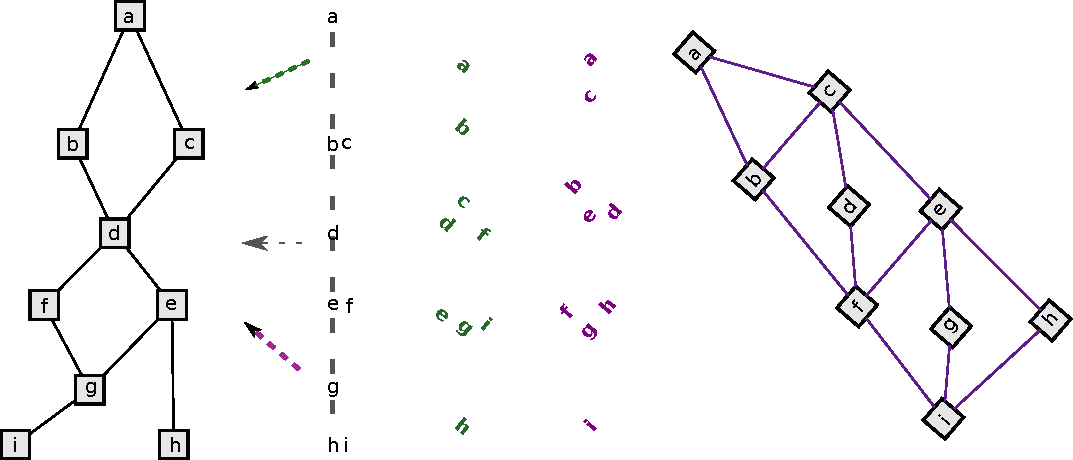
\includegraphics[width=0.7\linewidth]{/home/rudy/Documents/rudy/01_These/11_production/01_COMMUNICATION/figures/preferences_reseau_perspectives.pdf}
	\label{fig:preferences_perspectives}
\end{figure}
\figbox{
Lecture, de la représentation Fig.\ref{fig:preferences_perspectives}.
Dans quelle mesure des techniques différentes (agrégation complète, liste ordonnée ou réseau de préférences) et des perspectives différentes (figurativement avec l'inclinaison du réseau) ) modifient-elles les relations perçues entre entités et les décisions consécutives ?
Dans quelle mesure la perspective choisie sur les relations entre entités affecte-t-elle la décision\footnote{Il s'agit évidement d'une représentation figurative, les n dimensions alimentant la préférence ne sont pas réductibles à un plan de deux dimensions.} ?
Quelle est la réduction d'information minimale possible sans dépasser les seuils cognitifs et psychologiques ni déformé de façon inconsistante le jugement du décideur?
}


%\colorbox{yellow}{vers chap 4-5}

%\colorbox{yellow}{Reprendre exemple minimal avec le MMC1 de Rowley énergie coût}

%Il faut différencier les agrégations complètes pour le déterminer.
%\begin{itemize}
%\item Somme pondérée des indicateurs normalisés
%\begin{itemize}
%\item avec normalisation interne
%\item avec normalisation externe
%\end{itemize}
%\end{itemize}
%
%Cette analyse permettrait d'intégrer dans le corpus d'études soutenant la thèse d'une soutenabilité forte, des travaux sur des ''index`` de soutenabilité.
%Où comment concentrer l'information sur un indicateur unique ?
%Cela bien-sur est fait avec un grand nombre de dimensions.
%
%=> somme pondérée face à promethee face à AHP
%pressage de thèses :
%
%Moullec ? Génération de solution

Nous avons vu que l'intégration du jugement du décideur est un élément clef.
Pour présenter la question de la pluralité du corps décisionnaire, nous nous penchons sur les travaux d'\citeauthor{adla_aide_2010}.
Sans développer l'ensemble du contenu de \citetitle{adla_aide_2010}, nous observerons que la réussite d'un groupe vaste réside dans la maîtrise des communications synchrone, asynchrone, localisée et distribuée\footnote{Figure 3.3 : Quatre combinaisons des systèmes d’aide à la décision de groupe [Grudin 94], dans le Temps et l'espace~\cite{adla_aide_2010}}.

La prise en compte des parties prenantes visant la soutenabilité à l'échelle globale, tout en leur garantissant la protection de l'anonymat, \emph{est} la problématique du vote à distance (électronique).
Transparence, confidentialité, anonymat, unicité, sincérité, nous pourrions mettre tous ceci dans le cadre de l'expression du système de valeur pour la décision.
Et nous n'aurions aucun mal à reconnaître des travaux comme \citetitle{enguehard_vote_2007} de \citeauthor{enguehard_vote_2007}~\cite{enguehard_vote_2007} dans notre champ disciplinaire (ou interdisciplinaire).

La problématique de l'expression non biaisée dans les groupes distribués reste selon nous la question de `l'anonymisation-vérifiabilité' qui n'a pu être résolue jusqu'ici~\cite{pellegrini_chaines_2014}.
Il semble donc que notre espèce ne puisse accéder à ce stade de rationalité qu'en modifiant son comportement face aux expressions et au respect des opinions de chacun.e.s, pour accéder à la déclaration nominative.
Il serait naïf d'écrire cela ici sans ajouter qu'une telle occurrence est peu probable sans une horizontalisation des pouvoirs permettant de ne plus craindre d'action contre ces expressions d'opinions.
Par exemple, l'universalisation du salaire, libère de la contrainte à l'accès aux conditions matérielles d'existence.
Le tirage au sort aux fonctions de gouvernance (du local jusqu'au supra-national, tous pouvoirs confondus), libère des pressions des luttes partisanes et électives.
La co-propriété d'usage des moyens de production, libère de la subordination quant aux finalités et moyens choisis pour les obtenir.
Ne resterait donc que la coercition physique directe, difficilement extensible à de large ensemble (sous réserve des mécanismes cités précédemment).
Ces artefacts ne sont pas encore universellement appliqué ni reconnu.
Nous n'y sommes donc pas encore.


\subsection{Conclusion sur l'ADMC}
\label{concl:mcdm}

Nous avons vu au travers de cette présentation la diversité des méthodes disponibles, leurs caractéristiques et les fondements de l'\gls{ADMC}.
Nous avons ensuite traité la question des indicateurs (construction des critères) ainsi que leur formes d'agrégation, complète et partielle.
Nous en sommes venu au fait que la confrontation des deux approches doit distinguer les concepts faible et fort de la soutenabilité.
Mais en définitive, l'action de décision réside dans la mise en œuvre d'une unique alternative.
Même s'il peut s'agir de la combinaison d'alternatives, la combinaison elle-même reste une alternative unique.

La confrontation de l'école américaine et de l'école européenne (AHP, ELECTRE) est décrite par \citeauthor{lootsma_french_1990}~\cite{lootsma_french_1990}.
Elle relève par négatif les incohérences relatives aux approches de "l'évaluation objective".
C'est une indication sur l'acceptabilité de la subjectivité que nous retiendrons donc ici en conclusion.
\blockcquote[traduction]{lootsma_french_1990}{
La RAND Corporation, par exemple, une grande société de conseil américaine commanda le projet PAWN (pion) (analyse des politiques de gestion de l'eau pour les Pays-Bas, CF rapports de PAWN, 1981-1983) par l'autorité de gestion de l'eau néerlandaise `Rijkswaterstaat'
[.Elle (RAND)] a conçu un grand nombre de stratégies alternatives pour le contrôle des eaux de surface.
\emph{Ils ont rejeté l'analyse multi-critère pour la sélection finale d'une stratégie particulière, au motif que les décideurs devraient s'accorder explicitement sur les poids des critères et sur les scores des impacts.}
%The RAND Corporation, for instance, a large American consulting company commissioned with the PAWN project (Policy Analysis of Water Management for the Netherlands, see the PAWN reports, 1981-1983) by the Dutch water management authority Rijkswaterstaat, designed a large number of alternative stratégies for surface-water control.
%\emph{They rejected multi-criteria analysis for the final sélection of a particular strategy, on the ground that the decision makers would have to agree explicitly on the criterion weights and on the impact scores.
}
\keybox{
Ce qui fait obstacle à plus de rationalité dans les décisions humaines serait donc semble-t-il qu'il faille pour le décideur, être en accord avec son propre système de valeur et (pouvoir) l'assumer pleinement.
}
Toutefois, se maintenir dans l'irrationalité volontairement peut être d'autant plus préjudiciable que la solution sélectionnée peut être plus 'loin' (avec le système de valeur implicite), d'une solution plus rationnellement choisie avec le système de valeur explicite controversé mais transparent, comme d'un système plus consensuel ou d'un compromis explicité.

\keybox{
C'est en somme, au delà de l'acceptabilité de la complexité, une question de la légitimité du système de valeurs du décideur qu'il convient de résoudre pour que les \gls{ADMC}, de façon générale, et donc l'\gls{ACV} de façon particulière, soient acceptées.
} %section %%Intégrer la selection fuzzy mcdm mcda date d'ajout du 21/06/2016 avant 10h
%
\section{Conclusion sur les outils}
Qu'il s'agisse de la structuration de données ou de l'assistance à la prise de décision, la discipline de l'\gls{ACV} semble en retrait de ses sœurs aînées et voisines.
Les fondements théoriques sur la décision et la conception soulignent la criante inexistence du meilleur pour ne garder que la préférence.
Loin d'accepter dans sa majorité le rejet de \textit{l’intrinsèquement bon}, dans notre disciplines se trouvent des postures se révélant des archétypes~: du Traditionaliste dans l'appel à la simplicité, du Rationaliste constructiviste radical dans la défense de la meilleure alternative, et du Rationaliste attentiste se réclamant d'une soit disante \gls{ACV} objective de comptabilité.
Ces postures sont certainement des causes du piètre état d'élaboration des outils d'\gls{ACV} tel que vu dans ce chapitre au~\ref{sec:Outils de modélisation en ACV}.

L'\gls{ADMC} antérieure à l'\gls{ACV} a déjà entamé la liaison mais l'intégration semble lente et la communauté encore réticente 'au dépassement de la somme pondérée'.
La question du web sémantique, liées à celle de l'\emph{accessibilité des données}, cristallisant plus l'attention du praticien, dépassera peut-être la première de par le côté controversé du traitement de la subjectivité (négativement connoté) face au caractère sacré des \emph{données} dont nous sommes massivement friands et \emph{auxquelles certains d'entre nous abandonneraient même leur jugement}.

La conception fonctionnelle, semble avoir une implantation dans le tissu industriel des plus lente (au regard de sa lointaine naissance).
Sans doute est-elle aux prises avec les mêmes connotations que précédemment, puisque l'activité d'évaluation est en son sein.
Cela l'a d'ailleurs fort retardée, lorsque qualifiée d'art elle en fut (du moins un temps) dévaluée.
Elle n'en reste pas moins un outil essentiel à l'\gls{ACV} et un complément bien \textit{utile} à la décision multi-critère.

Le mouvement est lent mais les signaux sont forts concernant l'intégration de tout cela à l'\gls{ACV}.
Des cycles de re-conception méthodologique, structurés, disciplinairement soutenus et organisés sur les principes de l'open-source semblent à la fois prometteurs et en bonne voie. 					%chapitre
\chapter{ACV, la (re)conception d'un outil}
\label{chap:ACV, la (re)conception d'un outil}
Nous avons vu au chapitre sur les méthodes différents outils de conception.
Nous avons vu au premier chapitre l'état de l'art sur l'évaluation de la soutenabilité et les problématiques qu'il nous reste à résoudre.
Dans ce chapitre, nous ferrons la reconception méthodologique de l'ACV.

%\section{Méthodes de conceptions}

% ? literature review
% % 
% % \subsection{NLTK bibliography}
% % ? Do I develop the codes for analysing existing bibliometry and natural language metry ?
% % ? I would like to search for stems:
% % \begin{itemize}
% %  \item Allocation
% %  \item Normalisation / Normalization
% %  \item MCDA
% %  \item ISO
% %  \item ILCD
% %  \item compliant
% %  \item list of impact names and methods
% %  \end{itemize}
% %  
% % This work require: DL large amount of articles + scripting in python for searching troughs the publications
% 
% \subsection{External requirement analysis}
%\marginpar{
%{\tiny ? Est-ce que je rentre dans le détail AF comme part de l'AV (analyse de la valeur)
%Le plan de travail d'une action AV se décompose en 7 phases :...
%1) Orientation de l'étude
%2) Recherche d'informations
%3) Analyse fonctionnelle et analyse des coûts
%4) Recherche de solutions
%5) Étude et évaluation des solutions
%6) Bilan prévisionnel et choix
%7) Réalisation
%\cite{yannou_analyse_1998}
%> pas un journal ! autre ref}}

%\marginpar{
%{\tiny yannou analyse 1998 présent au .bib pas au bbl}}

L'analyse historique de l'\gls{ACV} est faite aux sections \ref{subsec:L'origine de l'ACV} et \ref{subsec:Historique de la méthode, son développement, son contexte}.
Nous n'irons pas jusqu'à présenter la phylogenèse\footnote{Histoire évolutive des espèces, ici histoire de l'évolution des techniques.} des outils de décision multi-critère pour y situer l'\gls{ACV}.
Nous remarquons toutefois au sein de l'historique deux choses~:
%\begin{enumerate}
%\item 
(i) Une période de formalisation et normalisation des pratiques est présente.
%\item
(ii) La \emph{démarche de conception} de la méthodologie de l'\gls{ACV}\ldots n'est pas décrite, ou du moins, nous ne l'avons pas identifiée.
%\end{enumerate}

Nous concevons nos objets et solutions techniques de nature matérielle avec une approche systémique.%~\cite{application de la conception fonctionnel dans le milieu industriel nourrir les ref}.
%\marginpar{{\tiny application de la conception fonctionnel dans le milieu industriel nourrir les ref}}.
%Historical overview was done in context.
%But within it, functional analysis of LCA seems missing.
%We design technical solutions answering needs of more materialistic nature with a systematic approach.
De la même manière, nous pouvons employer les outils de la conception pour produire les outils manipulant connaissances et décisions.
%In the same way we should apply a design methodology to produce the tools handling knowledge and decisions.
Il existe diverses méthodes de conception, telles que présentées section~\ref{sec:Méthodologies et théorie de la conception}.

Parmi ces méthodes de conception
%
%~\cite[Annexe 2: Méthodes de conception des systèmes.]{micouin_proposals_2006} depuis qu'elles ont été formalisée,
%%In the range of methods for design\cite[Annexe 2: Méthodes de conception des systèmes.]{micouin_proposals_2006} since it has been formalized since 
%vers 1920, selon \citeauthor{bayazit_investigating_2004},
%
nous resterons dans ce chapitre sur le socle commun des orientations du fonctionnalisme et du systématisme \textsc{la fonction}~\cite[section 4.1. Un concept commun, le concept de fonction]{micouin_proposals_2006}.
%, we will keep to the common ground from functionalists and systemics views~\cite{micouin_proposals_2006} \textsc{the function}.
Nous nous limiterons donc principalement à l'application de l'\acrlong{AF} décrite comme la troisième étape de l'analyse de la valeur~\cite{yannou_analyse_1998}, \textit{cf.} section~\ref{meth_conception}.

Nous proposons donc d'appliquer l'\gls{AF} à l'\gls{ACV}, d'observer les exigences techniques déduites, pour les comparer aux caractéristiques actuelles de l'\gls{ACV} (outils, normes, pratiques).
Quelques approches alternative compléterons ces vues.

Nous prendrons garde d'observer les niveaux pragmatique et informationnel (\textit{cf.} Tab.\ref{tab:ArchiSystEvaluation} section \ref{subsection:Éléments théoriques}).
Des niveaux qui jusqu'ici sont insuffisamment développés.
Le système informatique est assez détaché de l'utilisation et de l'échelle du système traité (système d'\textit{aide à la décision} sur un \textit{système global}).
De même ces niveaux sont peu traités par les références méthodologiques.
%We will apply external functional analysis (EFA) to LCA and observe the requirements deduced compared to the characteristics of currently used tools, standard and practices.

%L'issue de cette reconception théorique nous donnera les orientations poursuivies dans ce travail, à savoir~:(i) l'intégration du jugement dans l'ensemble des dimensions considérées et (ii) l'accès aux données.

Suivant les écarts qui apparaîtrons nous développerons dans les chapitres suivants les réponses fonctionnelles à ces besoins non comblés (\ref{chap:Multifonctionnalité} intégration du jugement de valeurs sur la multi-dimensionnalité concernée ; \ref{chap:Recherche Libre} disponibilité de la donnée).

%As a gap appeared, we propose to go further.
%Resulting of the EFA, we proposed to review the decomposition of mathematical construction of LCA, including the new stressed out elements.
%We based the formalism from the one describe by Heijungs and Suh g(B,A,f)~\cite{heijungs_error_2014}. OU CELUI DE JOILLIET (ECOSD) ?

%  potentially second article or specific section
% We should also consider Statistical analysis of current state of practice.
% check for text mining part of the article with the help of Chris.
% > Establishment of a glossary
% (based on specific vocabulary of LCA) and look at text analysis results. (cite potential TROPES / and Python NLTK)
% example:
% ~\cite{lynda} spatialisation
% allocation ; interpretation ; normalisation ; indicator selection

% other partnership with Murel for ecoinvent datasets and literature based datasets

%\section{Résultats}

\section{AF : Analyse Fonctionnelle, application}

Nous déroulerons l'\gls{AF} pour nous arrêter avant la rédaction du cahier des charges.
Nous ne le réaliserons pas ici puisqu'il s'agirait d'une écriture plus formelle, voir contractuelle, des sections \ref{subsec:besoin} à \ref{subsubsec:Caractérisation ACV}.
Nous ferons une simple incursion dans l'analyse des fonctions techniques via les \gls{FAST}.

%\end{tcolorbox}

%Une série de représentations graphiques est donc employée.
%We produced the analysis trough a set of graphical representations.

\subsection{Analyse du Besoin}
\label{subsec:besoin}
%\begin{center}\colorbox{yellow}{check terme de la NF}\end{center}
La première étape de l'\gls{AF} consiste en la recherche et l'énonciation du besoin.
Ce schéma du besoin figure~\ref{fig:diagramme_besoin}\footnote{La bête à cornes\textcopyright suivant la méthode APTE\textregistered.}, sert à poser les questions fondamentales déterminant l'objet~: (i) Qui~? (ii) Sur quoi~? (iii) Dans quel but~?
%First stating the goal of the artifact with the Horned Beast graph~\ref{fig:diagramme_interaction}.
\subsubsection{Le besoin derrière l'ACV}
\begin{figure}[htbp]
\centering
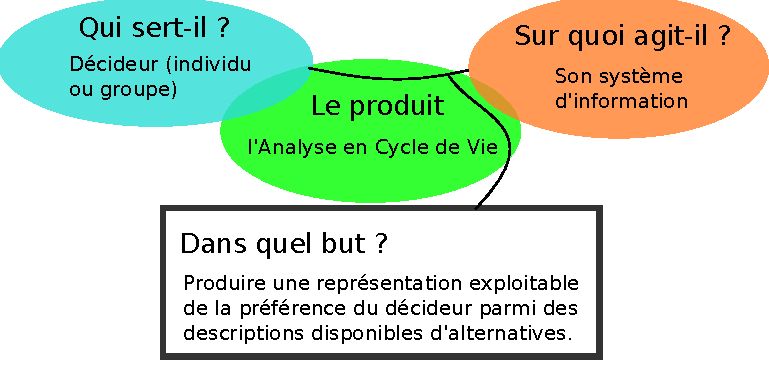
\includegraphics[width=0.7\linewidth]{/home/rudy/Documents/rudy/01_These/11_production/01_COMMUNICATION/figures/bete_a_cornes_201606.pdf}
\caption{Le schéma du besoin pour l'\gls{ACV}.}
\label{fig:diagramme_besoin}
\end{figure}

\figbox{                  
L'application du schéma du besoin à l'\gls{ACV} et la lecture de la figure~\ref{fig:diagramme_besoin}, nous donne l'expression du besoin fonctionnel suivante~:

Notre produit : l'\gls{ACV}, sert le décideur en agissant sur son système d'information dans le but de produire une représentation exploitable de la préférence du décideur parmi des descriptions disponibles d'alternatives.
\footnote{La notion de préférence est traitée au chapitre~\ref{chap:Méthodes et outils} section~\ref{sec:ADMC}, les interacteurs sont décrits dans la discussion suivante.}
}

\subsubsection{Discussion du Besoin}
%Discutons cette lecture pour en sonder ses limites.
L'\gls{ACV} établit une représentation de la préférence qu'aurait un décideur entre des différents états des aires de protection.
Les flux (échanges de produits et substances entre acteurs et milieux) modifient les états (impacts, dommages, satisfactions de fonctions),
\textit{cf.} le descriptif de l'\gls{ACV} \ref{sec:La pensée en cycle de vie}.
\paragraph{Réalisation d'inventaire.}
Questionnons nous à savoir si l'\gls{ACV} comprend ou non la réalisation des descriptions des flux, des systèmes et d'états.
Notons que nous ne pouvons déclarer de préférence vers des alternatives techniques ou organisationnelles que sur la base de leurs descriptions existantes.
C'est à dire que l'information disponible \emph{détermine} la préférence et potentiellement le choix du décideur.
\exbox{
Sur la base de 3 éléments d'information identiques, le classement des alternatives 'a' et 'b' donne $a P b$, (a est préféré à b).
%\marginpar{?notation symbolic logic}
Ces mêmes alternatives a et b sur la base de 4 éléments d'information peuvent parfaitement donner la préférence inverse $b P a$.

Prenons l'illustration de l'achat d'une paire de chaussure 
Vous ordonnez selon votre préférence les paires de chaussures A, B et C.
\begin{itemize}
\item Démarrons avec pour système de dimensions initial~: le système de fermeture, la couleur, la marque. L'ordre est alors~: CAB.
\item Introduisez le prix et l'ordre devient BCA car vous jugez C et A ``trop chères''.
\item Introduisez maintenant la pointure et l'ordre devient ABC où d'ailleurs BC vous sont inutiles car pas à votre pointure.
\end{itemize}
Cette exemple illustre que la valeur des critères (importance relative) conditionne le résultat.
}
\keybox{Il peut donc y avoir la nécessité d'acquisition de données (réalisation d'inventaires) pour répondre au système de valeur du décideur.}
\paragraph{Support de la décision.}
Nous soulignons également la prépondérance donnée au caractère décisionnel de l'\gls{ACV}.
Nous relevons en littérature la dichotomie entre \gls{ACV} de comptabilité et \gls{ACV} de décision.
Cette distinction y est à la fois mentionnée comme~:
\begin{itemize}
\item importante

\blockcquote[p.114, sec.2]{tillman_significance_2000}{Avec une distinction servant la différenciation entre étude rétrospective (comptabilité) et prospective (modélisation des effets du changement).}
%retrospective and prospective, or LCA with an accounting perspective and LCA modeling the effects of changes.
%The distinction between accounting LCAs and change-oriented LCAs is important.
%}
\item et comme artificielle

\blockcquote{weidema_application_1998}{puisque toute production d'information vise à affecter une décision}.
%It may also be argued that the distinction is artificial since the purpose of any information ultimately is to affect a choice, even for such a seemingly "neutral" application as "product declarations".}
\end{itemize} 
%Although it may be argued that all types of LCA are done with the same general purpose (i.e., environmental improvement, which in turn implies change), not all LCAs are made to support decision-making directly, in the sense of choice between formulated alternative actions. Decision-making may be described generally as a procedure where (1) a problem is formulated, (2) alternatives are formulated, and (3) a choice is made between alternative solutions to the problem [1]
%ref non accessible :
% Baumann H. Decision Making and Life Cycle Assessment. Licentiate thesis. Go ̈teborg:
%Chalmers University of Technology. Technical Environmental Planning Report 1995:4.
%(Also available as AFR Report 77. Stockholm: Swedish Waste Research Council.)


%argument court
%\begin{center}\colorbox{yellow}{Trouver formulation pour}\end{center}
%
%-
%
%Lors de ce type d'échange, je pense aux comptables et à leurs 'analyses'...
%"Ah, vous qui travaillez uniquement pour analyser.
%Ce n'est évidement pas pour que ces analyses servent à des décisions ultérieures."
%
%+
%
%L'information est dépendante de son contexte.
%Si je dis, ce produit vaut $35$ euros.
%Vous pouvez prendre cette donnée sur la base d'un consommateur et juger l'information acceptable.
%Si vous êtes parmi les industriels de la chaîne de valeur, ce n'est pas \textit{35} qui vous intéresse, mais $34.85$, car traitant de l'objet à des millions d'exemplaires, les décimales font valeur.
%L'information doit donc être lié à son contexte d'évaluation, son contexte de décision.
%
%-

\citeauthor{tillman_significance_2000} reconnaît d'ailleurs que 
%\footnote{
\blockcquote{tillman_significance_2000}{toutes les applications de l'\gls{ACV} visent le changement}.
%All these applications aim at change, or improvement: some in more direct ways (decision-making), some in more indirect ways, such as influencing market behavior or identifying improvement possibilities.}
%}.
La relations de la méthodologie de l'\gls{ACV} à son application est étudiée de longue date.
Elle réside dans le contexte décisionnel~\cite{wenzel_application_1998}.
%\footnote{
%\blockcquote{wenzel_application_1998}{The need to differentiate the LCA methodology when used in different applications derives from a limited number of variables. These variables all derive from differences in the consequence and the context of the decision to be taken.}
%}.
Puisqu'il y a donc reconnaissance d'une décision, directe ou indirecte, observons le point obtenant une reconnaissance commune~: \emph{l'évaluation}.

L'é\emph{valuation} est l'application d'un jugement de \emph{valeurs} sur des observations.
Or,\blockcquote[traduction]{gasparatos_embeded_2010}{dans la plupart des cas, le choix de l'outil d'évaluation est fait par le ou les analystes sans prendre en considération les valeurs des parties prenantes concernées.}
%In most cases, the choice of the evaluation tool is made by the analyst(s) without taking into consideration the values of the affected stakeholders.
%}
La séparation de l'évaluation et du processus de décision (et donc du décideur~: porteur du jugement) introduit d'après \citeauthor{grahl_evaluation_1996} une \textbf{contradiction}~:
%\footnote{
\blockcquote{grahl_evaluation_1996}{L'évaluation ne peut pas être déléguée en elle même. Si elle était déléguée sans le processus de prise de décision, une évaluation objective (i.e. sans jugement de valeur) serait requise -- une évidente contradiction dans ces termes.}
%The evaluation cannot be delegated on its own. If it were delegated without the decision-making process, an objective (i.e. value-free) evaluation would be required - an evident contradiction in terms.
%}
\label{grahl_impossible_deleguation}
Notez que nous distinguons délégation et séparation.
\exbox{Un couple visite des maisons en vue d'un achat.
La femme du couple, en technicienne avertie
 même si au chômage, 
% vient d'avoir une très bonne impression sur 
%préférera
apprécie une première visite
 d'un bien spacieux, dont les canalisations sont accessibles dans des vides techniques, où l'électricité vient d'être refaite aux normes et
 où seule la décoration reste à faire.
%  dont pour le coup toute la décoration est à faire puisque les murs sont nus dû aux récents travaux.
%Lors de la visite suivante, 
L'homme, %qui brûle de pouvoir enfin s'acheter sa demeure
grâce au poste en CDI dont il vient de valider la période d'essai, se projette 
%complètement 
lors d'une visite dans une charmante petite et \textit{ancienne} maison, avec son sol ancien, son parquet\ldots %et même la petite balancelle avec parasol sous la pergola où il s'imagine berçant l'enfant qu'il souhaite pour devenir Père.
%Il est maintenant hors de question pour lui de repenser 
%L'homme ne peut imaginer
%une contre-visite de ce qui lui est apparu comme un chantier poussiéreux et sans cachet qu'il a vu plus tôt.
%La femme pour ce second bien n'a que faire des sols dont elle sait devoir se défaire car le tout à l'égout n'est pas installé.
%Face à un bien où seul la décoration reste à faire, cette seconde maison \textit{ne vaut rien} (pour elle).

Hors de toute considération d'itérations ou contre-visite et si le décideur est le payeur, ce n'est pas la femme et son système (reste-à-faire, espace, fonctionnalité) mais l'homme qui actera, suivant le système (cachet de l'ancien, décoration, ``ressenti'').

%L'évaluation de madame peut être tout à fait exacte face à son système de valeur (travaux, reste-à-faire, fonctionnalité).
%Toutefois, s'ils avaient à signer dans la seconde et si \emph{le} décideur, avec pour système, le cachet, la décoration, ``le ressenti'' devait apposer son accord, c'est sur le second bien qu'il se lancerait.

Système de valeurs évaluateur et système de valeurs décideur ne font qu'un.}

Nous affirmons, comme \citeauthor{grahl_evaluation_1996},
que l'é\textbf{valua}tion n'est pas \textbf{séparable} des \textbf{valeurs} et donc du \textbf{décideur} (porteur des valeurs qui acte le choix).
Mais nous développerons ultérieurement notre proposition afin de permettre la \emph{délégation} (\ref{délégation de valeurs2}).

Terminons donc par la phrase conclusive de \citeauthor{grahl_evaluation_1996} sur cette question~:
\keybox{
\blockcquote[traduction]{grahl_evaluation_1996}{Les \gls{ACV} sont donc des aides à la prise de décision, mais pas un substitut aux décisions elles-mêmes.
%LCA's are thus a decision-making aid, but no substitute for the decisions themselves
}
}

Il en résulte l'\textbf{expression du besoin}, à remplir par l'ACV~:
\keybox{
Produire une \underline{représentation exploitable} de la \underline{préférence du décideur} (personne ou groupe) parmi des \underline{descriptions disponibles d'alternatives}.
}
Les groupes nominaux (soulignés) de cette phrase seront les éléments clefs de la contribution de ce mémoire.
Les descriptions disponibles traitent de la disponibilité de la données, de sa mise en formes pour un traitement dans le volume nécessaire (Chap.~\ref{chap:Recherche Libre}).
Les représentations exploitables sont celles issues des techniques d'\gls{ADMC}, qui visent à rester dans nos capacités cognitives.
La préférence du décideur est l'objet que nous intégrons dans l'\gls{ACV} par nos travaux, d'abord avec ce qui fut jusqu'ici positionné dans l'étape d'inventaire (i.e. allocation Chap.~\ref{chap:Multifonctionnalité}), puis de façon générale dans l'interprétation (Chap.~\ref{chap:Jugements et Multi-dimensionnalité}).

%{\color{BlueViolet} Our product, or artifact : LCA,} serves {\color{SkyBlue}its user (human for now)} acting on {\color{Goldenrod}the information system} in order to produce a representation of preferences between alternatives according to the decision makers (human) value system.

% \tikz[baseline=(n1.base)]{\node[fill=green!20,rectangle] (n1) {Our product, };}\tikz[baseline=(n1.base)]{\node[fill=green!20,rectangle] (n1) {or artifact : LCA};} serves \tikz[baseline=(n1.base)]{\node[fill=green!20,rectangle] (n1) {its user (human for now)};} acting on \tikz[baseline=(n1.base)]{\node[fill=green!20,rectangle] (n1) {the information system};} in order to produce a representation of preferences between alternatives according to the decision makers (human) value system.

\subsection{Analyse fonctionnelle du besoin (\acrshort{AFB})}
Après avoir clairement identifié le besoin, il faut ensuite décrire en termes de services les nécessités (exigences) pour y répondre.
Il s'agit de \emph{nécessité} au sens large.
\exbox{Ainsi seuls les produits fabriqués (et donc ceux que l'on peut produire), ou naturellement existant, délivrent leurs services.
De même, un produit ne permettant pas le traitement des ses déchets en fin de vie obstruerait et pourrait dégrader nos sociétés.
%Ce qui à termes entraînerait son abandon.
Mais les nécessités réglementaires ou culturelles sont à prendre en compte également.
Imaginez un grill de bœuf en Indes, ou des cendriers de bureau après la loi Évin en France.}
\keybox{
C'est donc la même logique, en cycle de vie et multi-dimensionnelle, qui parcours l'\gls{ACV} et l'\gls{AF}.
}
\subsubsection{Identification des phases de vie du produit}
Usuellement cette étape de l'\gls{AFB} démarre par la distinction des phases de vie du produit.
S'agissant d'une méthodologie nous distinguons les phases suivantes~:
\begin{itemize}
\item Élaboration (conception)
\item Utilisation (application)
\item Fin de vie (fin d'exploitation, obsolescence)
\end{itemize}

Parce que nous sommes dans l'élaboration et que nous n'envisageons pas de dispositif post ACV, nous concentrerons l'étude à l'étape d'utilisation.
Permettons nous toutefois de passer synthétiquement sur ces autres étapes.

L'\textbf{Élaboration} concerne notre travail même.
Cette étape comprend donc dans son milieu extérieur la communauté contribuant à la méthodologie de l'\gls{ACV}.
Nous réfléchissons donc à l'établissement d'une méthodologie de décision visant plus de rationalité et donc un encrage dans notre connaissance du réel dans son périmètre le plus étendu possible (holisme\footnote{Qui considère les objets observés comme un tout.}).
\blockcquote[traduction]{lenoir_curricular_2015}{Plus largement, c'est une indication d'une orientation de nos sociétés occidentales, [\ldots]
%plus que l'émergence de cette orientation:
Ce n'est pas l'émergence d'une façon d'aborder la connaissance de plus en plus divisée, mais plutôt le signe d'une préférence pour la prise de décision éclairée, basée sur des vues techniquement fondées, et sur la volonté de prendre des décisions sur la base des scénarios étayées par des connaissances spécifiques.
Voilà pourquoi l'interdisciplinarité trouve des points d'ancrage dans toutes les sciences appliquées, sociales ou autres. (Sinacœur, 1983, pp. 25-26)}
%More broadly speaking, it is an indication of an orientation of our Western societies, more than the emergence of this orientation:
%It is not the emergence of a way to address increasingly separated knowledge, but rather the sign of a preference for informed decision making, based on technically founded views, and on the desire to make decisions on the basis of scenarios underpinned by specific knowledge. This is why interdisciplinarity finds anchoring points in all the applied sciences, social or other. (Sinacœur, 1983, pp. 25-26)
%}

Il s'agit d'établir les fondations méthodologiques d'une méthode d'évaluation pour la décision (science de gestion) holistique (spectre complet des sciences naturelles), dans la limite des capacités cognitives humaines (neuro-psychologie) et respectueuse du jugement de valeur du décideur (socio-psychologie) applicable à diverses cultures et par elles (sociologie - anthropologie - linguistique).

Il s'agirait donc pour la conception la plus robuste de l'\gls{ACV}, que l'ensemble des disciplines et acteurs mis en œuvre soient sollicités.
%C'est pour partie l'explication de l'étalement disciplinaire de ce mémoire. % traitement des ajouts du 20/06 à zotero
C'est l'un des points de l'argumentaire sur la disponibilité de la donnée (de toutes les disciplines et donc sans barrières entre-elles).

Le milieu extérieur de cette étape comprend également les praticiens actuels.
Nous relevons un conflit d'intérêt important pour les acteurs économiques dont la \emph{reproduction}\footnote{Au sens marxiste du terme, la reproduction des forces de travail.} tient dans la capacité à vendre des prestations d'\gls{ACV} à d'autres acteurs.
Il nous paraît conflictuel à la fois, de produire des réflexions sur une méthodologie comportant plusieurs problèmes non résolus à chacune de ses étapes et de vendre l'application, ou des données pour l'usage, de ladite méthodologie.
Malgré tout, les praticiens les plus expérimentés (et donc à même de juger l'opérationnalité de l'artefact reconçu), sont ceux-là même qui applique la méthodologie actuellement déficiente et qui donc sont psychologiquement et économiquement dans la position la plus délicate pour la remettre en question.

La \textbf{Fin de Vie} de l'\gls{ACV}.
Sur les conditions d’obsolescence de la méthodologie de l'\gls{ACV}, nous ne pouvons que conjecturer sur les évolutions du système d'information, des décideurs, de leur capacités cognitives et de notre organisation sociale face aux choix.
Nous nous abstiendrons de développer ces questions.

Nous observons toutefois que l'étude d'une décision apparaît lorsqu'elle est prise, mais également après, en justification ou plus ultérieurement encore, pour la comprendre.
Cette dernière raison, celle de l'historien nous concerne peut-être peu, si ce n'est que pour demander à ces spécialistes les problèmes qu'ils anticipent dans la compréhension pour les générations futures de nos décisions passées.
C'est à dire ``Que devons nous anticiper relativement à l'élaboration méthodologique de l'\gls{ACV} pour que nos enfants puissent (i) s'en saisir (ii) juger effectivement la méthode obsolète ?''.
Nous ne connaissons pas par avance le contenu qui sera produit.
Cependant, ici encore, il s'agira d'argument en faveur de la \emph{libre} transmission des connaissances pour les générations futures.

Nous poursuivons donc la démarche avec l'étape d'\textbf{Utilisation}.

\subsubsection{Caractérisation en phase d'utilisation de l'\acrshort{ACV}}
\label{subsubsec:Caractérisation ACV}

\paragraph{Identification et caractérisation des \acrlongpl{EME}}

\subparagraph{Distanciation à la représentation classique de l'\gls{ACV}.}
\label{par:Distanciation à la représentation classique de l'ACV}
Nous retrouvons dans les \acrlongpl{EME}, des éléments centraux tels que le décideur et le système d'information mentionnés à l'étape précédente.

Nous avons bien entendu pensé au système de représentation classique de l'\gls{ACV} et du développement durable (\textit{cf.} section~\ref{sec:La pensée en cycle de vie}).
Toutefois la mention d'\gls{EME} comme écosystème, ressources économiques, sphère sociale, ne nous paraissait pas opportune.
En effet, nous considérons que l'\gls{ACV} inter-\emph{agit} avec un système d'information et non ces éléments pré-cités.
L'\gls{ACV} ne touche pas directement les produits, services ou procédés,
car elle n'est pas en contact avec le système observé.
Elle n'est en liaison qu'avec l'information relative au système observé.
Ainsi, l'élément d'interaction est ici le système d'information.

Il est apparu délicat de dissocier la méthodologie de l'\gls{ACV} et le système d'information nécessaire à la réalisation de l'\gls{ACV}.
La question est de savoir si le système d'information est un \gls{EME}.
Or, ce sont bien les caractéristiques méthodologiques de l'\gls{ACV} qui imposent un certain système d'information.
Les caractéristiques précises n'en seront que la traduction en solutions fonctionnelles puis techniques.

Les éléments cités précédemment (\gls{technosphere}, \gls{biosphere}\ldots) ont une forte présence dans la perception actuelle de l'\gls{ACV}.
%Nous tenons donc à permettre au lecteur de visualiser le traitement de cette question.
%Il nous semble donc important de détailler ce point.
%Pour cela nous l'invitons à consulter 
La figure \ref{fig:information_sys},
représentation du système technique, social, économique, vise à proposer une articulation moins simpliste que l'actuel dichotomie technosphère écosphère.
Nous y questionnons notamment la position du système d'information. % ainsi qu'à illustrer le rapport de ces objets au système d'information.

\begin{figure}[htbp]
\centering
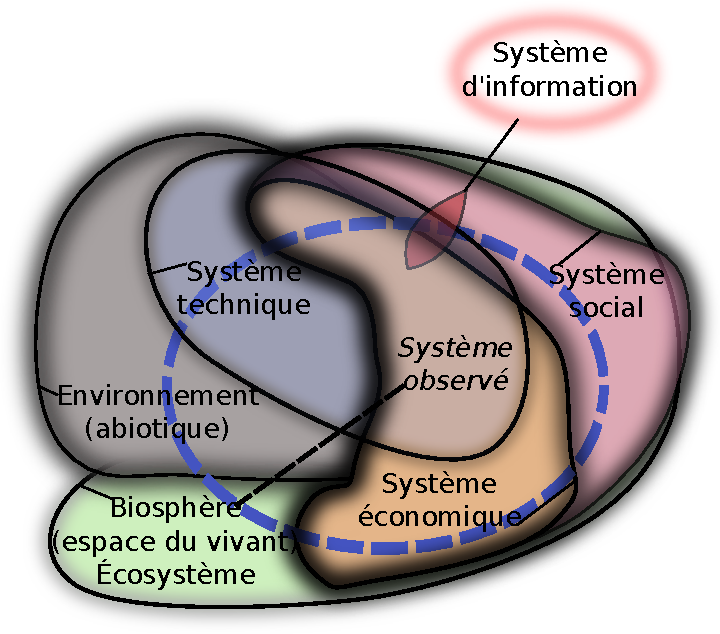
\includegraphics[width=0.7\linewidth]{/home/rudy/Documents/rudy/01_These/11_production/01_COMMUNICATION/figures/systeme_d_information_et_ACV.pdf}
\caption{Représentation alternative pour l'\gls{ACV} des systèmes, techniques, sociaux, économiques et de l'écosphère.}
%Second step in external functional analysis, listing the elements of the artifact's environment and describe its relations trough functions. Either users i.e. functional requirements of constrains. Here only use phase is considered.

\label{fig:information_sys}
\end{figure}

\figbox{
Sur la figure \ref{fig:information_sys}, on observe les différents éléments habituels relatifs à l'\gls{ACV} et décrit à la section~\ref{subsubsec:Vocabulaire de base}~: La biosphère, l'écosphère, la techno-sphère ; mais aussi le vocabulaire des méthodes d'impacts~: les ressources abiotiques, biotiques, l'environnement social.
Un trait relie le périmètre et sa désignation.
Ni les contours, ni les libellés n'ont vocation ici à être exactes.
Ils ne servent qu'à pousser au questionnement.
\exbox{Existe-t-il une part du système technique, qui ne serve pas la répartition des ressources ($\overline{\mathit{système~économique}}$)? , qui ne traite pas des relations entre individus ($\overline{\mathit{système~sociale}}$)?\ldots}
%Nous employons le flou pour indiquer l'incertitude épistémologique et la transparence des surfaces indique la non exclusion des domaines entre eux.

Cette représentation comprend volontairement pour le système observé un contour pointillé et de périmètre inférieur aux différents ensembles, techniques sociaux et environnementaux.
La transparence des surfaces indique la non exclusion des domaines entre eux
En effet, une des difficultés de l'\gls{ACV} est de ne pouvoir traiter que du champ connu des systèmes sans connaître la proportion de cette part dans ces systèmes.
Ces \textit{extérieurs au domaine connu} sont représentés avec un contour flou signifiant notre incertitude épistémologique\footnote{\href{http://www.uved.fr/fileadmin/user_upload/modules_introductifs/module3/risques/1.3/html/2.html}{Hyperlien vers la documentation des formes d'incertitude}.}.

La frontière commune du système social et économique vise à souligner que l'organisation des relations humaines, en général ou en particulier pour la gestions de ressources (économie), repose sur un même et unique encrage matériel.

Au sein de l'\emph{écosphère} l'homme s'est organisé en \emph{société} et a déployé des \emph{systèmes techniques}.
Une partie de ce système socio-technique (vivant et non-vivant, matériel) est le système d'information.
Nous considérons le système d'information comme la combinaison des systèmes techniques (incluant de ressources abiotiques) et de systèmes sociaux (comprenant les personnes -- compris dans l'écosystème -- travaillant au sein de celui-ci), visant l'information.

%L'homme observant l'écosphère ainsi que lui même produit l'observation.
Le système observé est la fraction de l'écosphère inscrite au système d'information.
%Toutefois toutes les données relatives au système d'information ne sont pas nécessairement incluses à l'information dans ce système.
Le système d'information n'observe donc qu'une partie de l'écosphère, du système socio-technique et de lui même.
\emph{C'est cette partie qui est exploitable pour la prise de décision.
Il ne faut donc pas oublier de quels composants (humains et techniques) elle découle.}

Une fois rendu plus souples dans nos perceptions catégorisées de notre environnement, nous pouvons franchir l'étape suivante.
La décision affecte par partie ou dans son ensemble les différents systèmes entremêlés.
Qu'importe qu'il s'agisse d'un espace que l'on qualifie d'éco-bio-techno-sphère, que les éléments affectés soit biotique ou non.
Des états sont modifiés, les étiquetages qu'il est possible de réaliser ne doivent servir qu'à l’assistance du décideur pour 'situer' sa préférence.
%C'est sur elle que porte l'évaluation.
% texte des différents domaines
%Ressources non employées dans les systèmes techniques
%Y a-t-il des systèmes techniques ne servant pas à la gestion de ressources ?
%Vide si l'on considère les ressources pour le système technique.
%Système de gestion des ressources (non uniquement monétaire)
%L'écosystème (biotique et abiotique) observé fait-il nécessairement part du système sociale ou non ? Nous partons sur le principe que non.
%Commerce du vivant (agriculture, sylviculture, élevage, travailleurs)
%Un système technique peut-il être hors de notre système sociale ? Une épave de navire
%Vide suivant que l'on considère le domaine du vivant avec ou sans son support matériel
%Vide pour ceux de croyance athée.
%? noosphère
%\begin{center}
%\colorbox{yellow}{Trouver un formalisme sur la symbolique des ensembles ?}
%\end{center}
%
%$homme \in vivant \in biosphère \in ecosphère$
%
%$ecosphère - biosphère = abiotique$
%
%$système technique = $
%\end{tcolorbox}
}
Cette représentation complexe est simplifiée pour la figure~\ref{fig:octopus_LCA}.
Il n'y a, par exemple, dans cette seconde figure pas d'intersection entre système technique et écosystème (biosphère).
Or tout système agricole comprend des outils (abiotique) et des outils vivants (biotique)\footnote{Le terme dans ce cadre est `auxiliaire de culture'}.
Cette représentation doit toutefois déjà nous éclairer pour dépasser notre dichotomie classique \Gls{technosphere} | \Gls{ecosphere}.

\subparagraph{Les \gls{EME} de l'\gls{ACV}} considérés sont donc pour cette étape "utilisation" et sur cette base de l'interaction avec un système d'information, les \gls{EME} de la figure~\ref{fig:EME-ACV}.
\begin{figure}[h]
\centering
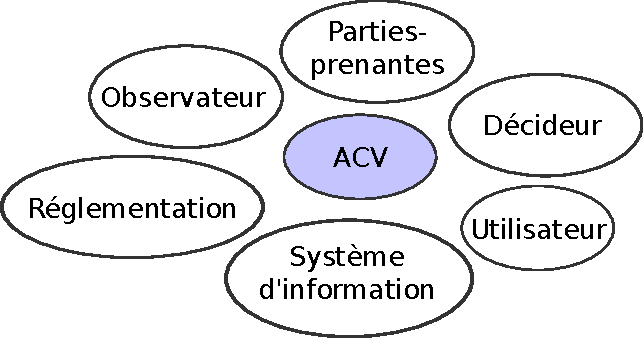
\includegraphics[width=0.8\linewidth]{/home/rudy/Documents/rudy/01_These/11_production/01_COMMUNICATION/figures/EME.pdf}
\caption{Éléments du Milieu Extérieur de l'\gls{ACV} en phase d'utilisation.}
\label{fig:EME-ACV}
\end{figure}
\figbox{
Le schéma des EME de notre application est la représentation fig.~\ref{fig:EME-ACV}.
Ce type de schéma comprend généralement~: l'utilisateur, l'observateur, la réglementation, la matière d'œuvre et le milieu environnant.
Nous omettons volontairement ce dernier (environnement). celui-ci conduit aux fonctions de résistance au milieu (usuellement caractéristiques de corrosion, résistance UV\ldots).
Ce choix réside dans le fait que nous n'éclairons pas les caractéristiques géographiques et matériels en support à la méthodologie (réseaux de communication, appareillages).
Nous ne faisons pas ici l'\gls{AF} du matériel d'un système d'information supportant l'\gls{ACV} mais celui de la méthodologie de l'\gls{ACV} elle-même.
Ceci implique que notre caractérisation portera sur la méthode et les caractéristiques du traitement de l'information (logique, cognition, mathématiques, légales\ldots) et pas sur la condition matérielle de l'application de l'\gls{ACV} (data-center, nature des réseaux de communication, volume de données, vitesses de calculateurs\ldots).
%Nous comprenons cependant l’existence de limites techniques quant à la capacité de calcul et de stockage requise.
%Mais ces éléments sont simplement hors de notre champ de compétences.

Ainsi pour notre analyse, les EME sont~: La réglementation, l'observateur, les parties-prenantes, le décideur, l'utilisateur et le système d'information.
%Nous serons amener à faire évoluer ces représentations au fil du travail.
}
\paragraph{Identification des Fonctions de Services (F.S.)}
Analysons maintenant les relations entre l'\gls{ACV} et ses EME.
Cette analyse est facilitée par la représentation graphique du diagramme des interacteurs, figure~\ref{fig:octopus_LCA}.
%dans ces phases de vie.
Ceci nous guide dans l'identification des fonctions que doit remplir l'\gls{ACV} et la définition de ses caractéristiques consécutives.
%Then analyzing the relation between LCA (our artifact) and its environment, trough the octopus graph~\ref{fig:octopus_LCA}, guides us toward the characteristics such tool shall possess.


\begin{figure}[htbp]
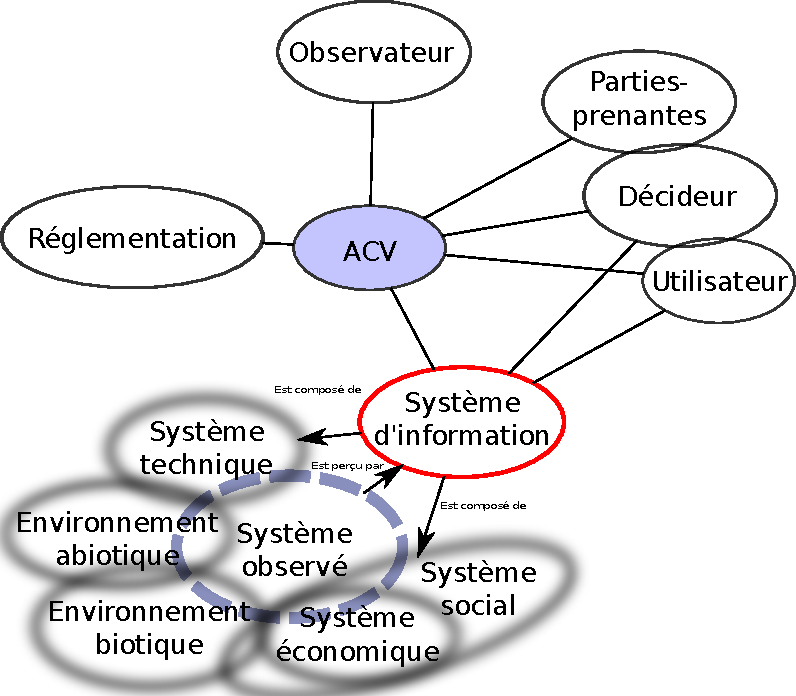
\includegraphics[width=\linewidth]{/home/rudy/Documents/rudy/01_These/11_production/01_COMMUNICATION/figures/octopus_ACV.pdf}
\caption{Représentation des éléments de l'environnement du produit en interaction avec lui (phase d'utilisation).
%Second step in external functional analysis, listing the elements of the artifact's environment and describe its relations trough functions. Either users i.e. functional requirements of constrains. Here only use phase is considered.
}
\label{fig:octopus_LCA}
\end{figure}

\figbox{
La figure~\ref{fig:octopus_LCA} est lu de la façon suivante.
Nous débutons par une représentation des éléments classiques de l'environnement incluant la réglementation, l'observateur et l'utilisateur.
Chacun exerce à minima une contrainte sur l'objet à concevoir, représentée par un trait simple fig.~\ref{fig:octopus_LCA}.

Deux \gls{EME} agissent sur la matière d’œuvre, l'utilisateur et le décideur.
Nous commençons par lier d'un trait droit ces \gls{EME} et le système d'information.
La suite de la caractérisation déterminera la nature de ces relations lorsque nous préciserons en quoi l'ACV modifie ces liaison entre acteurs et matière d'œuvre\footnote{Puisque nous sortons du cadre classique des représentations d'\gls{AF}, nous pouvons souligner qu'il pourrait être intéressant d'illustrer d'autres relations entre \gls{EME}, par exemple l'interaction entre des parties-prenantes et la réglementation.
Lors de recherche ultérieures, cela apportera peut-être de nouvelle thématiques de recherche, comme des pratiques de conception.}.
}

Nous allons donc observer et \textbf{décrire chaque \gls{EME}} puis détailler les relations à l'\gls{ACV}.
Ces observations nous permettrons ensuite de \textbf{formuler des exigences fonctionnelles} pour la caractérisation des fonctions de l'\gls{ACV}.
Les exigences seront listées indépendamment de leur redondance à d'autres \gls{EME}.
\exbox{Être compréhensible, d'un observateur comme de l'utilisateur par exemple.}
Une exigence fortement redondante est normalement adressée avec une plus forte priorité.
Ceci se traduit par des niveaux plus strictes des critères relatifs à ces fonctions.
%If we detail the relationship between LCA and its environment we can state the following elements.

\subparagraph{Le Système d'information}
\label{subparagraph:Le Système d'information}
\subparagraph{Description de l'inter-acteur~:}

Nous avons développé la représentation relative au système d'information figure~\ref{fig:information_sys}, car c'est un élément central.
\emph{Parce que le système observé est vaste, dynamique, global et complexe, le système d'information est (devrait être) à son image.}
Nous tendons à diviser le système observé en techno-sphère, biosphère en système social et économique.
Ce faisant, nous oublions qu'il ne s'agit que d'une seule et même réalité.
Cette représentation est donc une construction arrangeante pour la comptabilisation de flux au travers de frontières.
Le volume de contrôle déterminé par l'interaction humaine visait à identifier des flux élémentaires (générateur d'impact) et des flux produits établissant la chaîne de valeur.
Or, des indications sont observées à la fois dans et hors du volume de contrôle.
De plus, la caractérisation des impacts nécessite une localisation plus fine que "rejet dans la biosphère".
Ceci est observé à travers la sous-compartimentation déjà existante et croissante, disponible en méthodes d'impacts et dans les travaux sur la spatialisation~\cite{yan_ontology_2015}~:
eau~: douce, marine ; air~: forte densité de population, faible densité de population \ldots
%\begin{itemize}[noitemsep,topsep=0pt,parsep=0pt,partopsep=0pt]
%\item eau
%\begin{itemize}[noitemsep,topsep=0pt,parsep=0pt,partopsep=0pt]
%\item douce
%\item marine
%\end{itemize}
%\item air
%\begin{itemize}[noitemsep,topsep=0pt,parsep=0pt,partopsep=0pt]
%\item forte densité de population
%\item faible densité de population
%\end{itemize}
%\item sol
%\end{itemize}
%\ldots

Nous ne devrions pas rester prisonniers d'une partition d'un système que nous avons nous même établi.
Il faut alors comprendre et accepter la multitude de perceptions du système dans lequel nous somme immergé.
Cela peut être le résultat d'une multitude d'opinions issues d'une même perspective culturelle ou par l'intégration d'une multitude de perspectives culturelles.
Il faut donc laisser à l'utilisateur de la méthode d'\gls{ACV} et aux développeurs la possibilité de déterminer les caractéristiques du(des) volume(s) de contrôle.
Si un décideur considère plus importante une région géographique particulière, les caractéristiques méthodologiques de l'\gls{ACV} (dans ses normes comme ses outils) ne doivent pas y faire obstacle car ce serait faire obstacle au système de \emph{valeurs} à appliquer et donc à l'é\emph{valuation}.


\subparagraph{Exigences~:}
 
 Les attributs de la structure de connaissances, du système d'information utilisé doivent être~:
 
 \begin{itemize}[noitemsep,topsep=0pt,parsep=0pt,partopsep=0pt]
  \item Adaptabilité. Doit pouvoir être adapté aux écarts linguistiques et culturels, donc permettre le traitement de multiples ontologies.
  \item Interactivité. Doit être caractérisé par l'absence ou la limitation la plus importante possible de barrières et couloirs d'étranglement à la production, la mise à jour et la correction.
  \item Robustesse. Doit être équipé des outils les plus avancés de manipulation et sauvegarde des données et de leurs versions.
  \item Globalité. Doit être développé avec de multiples standards de communication. Doit être accessible et fourni à travers le globe et éditable depuis chaque endroit.
  \item 'Scalablilité'. Doit permettre de faire face au gigantisme de la masse d'information à traiter. %la lisibilité par machine en vue
  \item De complétude minimale. Doit contenir l'ensemble de l'information minimum à l'exercice de la fonction de l'\gls{ACV}.
  Ici nous devons disposer \emph{à la fois} les descriptions objectives et des valeurs (opinions) avec une distinction claire des deux natures d'information stockées.
 \end{itemize}


%\begin{description}
% \item Information system:
% 
% LCA does not touch the products, services, processes.
% LCA is not in contact with the system observed.
% Its relates to information about the observed system.
% So the element LCA interacts with, is the information system.
% We developed it here because it is a central element.
% And as the observed system is vast, dynamic, global, complex, the information system is (must be) to its image.
% We tend to divide the observed system in techno-sphere, biosphere, social, economical systems.
% And doing so we start to forget it is a single one reality.
% It is a convenient construction in order to account flows to rise borders.
% But we should not remain entangled within one perceived partition of the system.
% We must also comprehend the varying perception of the system.
% May it be with wide-ranging opinions from the same cultural perspective or by the integration of wide-ranging cultures.
 
% Requirement:
% 
% The knowledge structure and information system used must be:
% \begin{enumerate}[noitemsep,topsep=0pt,parsep=0pt,partopsep=0pt]
%  \item Versatile. That can be adapted to mind the language or cultural gaps and encompass multiples ontologies.
%  \item Highly interactive. Limited or absence of up-dating and correcting bottle neck(s).
%  \item Robust. Equipped with state-of-the-art versioning management and safeguards tools.
%  \item Globalized. Developed with multiples and/or widely used communication standard, globally accessible and locally supplied all around the globe.
%  \item Scalable, machine readable (to face the gigantism of data to handle).
%  \item Withhold both descriptions and value systems with clear distinction.
% \end{enumerate}

%   \end{description}


\subparagraph{La Réglementation~:}
 \subparagraph{Description de l'inter-acteur~:}
 L'\gls{ACV} manipule des données.
 En conséquence, cet outil doit conduire au respect des droits d'auteurs et diverses propriétés relatives à ces informations.
 L'\gls{ACV} a une forte intensité en données qui nécessitent de pouvoir être utilisées, modifiées, distribuées, pour la vérification et curarisation.
 Ces opérations doivent pouvoir se faire avec le moins de résistance possible, résistances légales incluses, sans pour autant contrevenir aux législations.
 
% Ces notions sont éclairées par le travail de \citeauthor{beitone_biens_2010}.
% Il nous faut les appliquer aux éléments manipulés en \gls{ACV}.
% L'\gls{ACV} agit sur les systèmes d'information, pas autre chose.
% Les conditions appliquées à ces informations, leur « licence », déterminent ce qui peut être fait de l'\gls{ACV}.
% 
% \begin{tabular}{ p{5cm} p{5cm} p{5cm}}
% 	\hline
% 	& Excluabilité & Non excluabilité \\
% 	Rivalité & Biens privatifs & Biens communs \\
% 	Non rivalité & Biens de club & Biens collectifs \\
% 	\hline
% \end{tabular}
% 
% Comme les lecteurs l'auront constaté en état de l'art, les biens de club sont la majorité en \gls{ACV}.
  
 Le traitement des informations qui portent sur les préférences et opinions, nécessite la protection des personnes qui les expriment.
 \emph{Il est également nécessaire d'apporter une protection contre l'unification et la standardisation des systèmes de valeurs comme outil d'hégémonie, par exemple~: l'obligation légale d'application d'un système de valeurs unique identifié.}\footnote{Sans quoi nous ne respectons pas l'ensemble des composants de la définition de soutenabilité, \textit{cf.} Sec.~\ref{sec:La Soutenabilité}.} %(http://www.cnrtl.fr/lexicographie/h%C3%A9g%C3%A9monie)
  
 %
 % \item Regulations:
 % 
 % LCA handles data.
 % So a legitimate consequence is that using LCA must respect authors properties rights.
 % LCA being data intensive, it needs to be able to use, modify and distribute a lot of data with as less resistance as possible.
 % The diffusion of information on preferred values (and as a results systems) generate protections or weaknesses.
 % Protection against unification or standardization of value systems as hegemonic weapons should be carefully studied.
 % What would be the consuming behavior with alternative regulation on supplementary information ?
 % As an example, try to picture your reaction with \ref{fig:declaration_soutenable_pdt}.
 
\exbox{
 Nous illustrons l'étude de cet \gls{EME} avec les déclarations environnementales de type III\footnote{Les déclarations environnementales actuelles sont déclinées en I écolabels, ISO~14024 (certification)~;
 II auto-déclaration, ISO~14021 (déclaration à la responsabilité du producteur)~;
 III éco-profils ISO~14025, communication de résultats d'ACV.}.
 Faisons l'hypothèse d'une réglementation rendant obligatoire le type d'affichage proposé dans le modèle ATLETTE II (Appliance Testing for Washing Machines Energy Label \& Ecodesign Evaluation)~\cite{therese_kreitz_atlete_2014}.
 Quel serait le comportement de consommateur avec une réglementation alternative sur l'information complémentaire obligatoire sur les produits de grande consommation (propositions fig.~\ref{fig:declaration_soutenable_pdt})~?
 }
 
 Une personne prend naturellement (sans assistance) un mode de raisonnement heuristique~\cite{meyer_modetraitement_2000}.
 C'est à dire qu'une sélection de l'information employée pour la décision est opérée sur la base de l'expérience (des pré-jugés) de la personne.
 Ceci dans le but de réduire l'énergie consommée, le coût cognitif.
 \blockcquote{meyer_modetraitement_2000}{Nous traitons l'information la plupart du temps selon un principe de moindre effort (Allport, 1954) et de suffisance
 (Simon, 1976) par rapport aux buts du traitement.}
 
 Les habitudes des consommateurs traitent nécessairement du prix et ses variations.
 Un affichage traitant des notions habituelles, non-techniques et émotionnellement liées aux sujets, pourrait avoir une influence bien plus importante sur son choix.
 Nous ne limitons d'ailleurs pas nos hypothèses d'application au EuP-ErP (produit utilisateur d'énergie ou lié à l'utilisation d'énergie).
 Nous reprenons donc dans un premier exemple pour illustrer ce propos, les travaux de Gaël \textsc{Gireau} (facteur 12)~\footnote{Ces travaux traitent de l'encadrement des salaires. Ce type de questionnement en économie à d'ailleurs fait l'objet d'une votation en Suisse~\cite{chancellerie_federale_suisse_votation_2013,gadrey_ecarts_2013}}.
 Un étiquetage visant la soutenabilité pourrait par exemple reprendre l'écart salarial sur l'ensemble de la chaîne de valeurs (supply chain).
 Ainsi, imposer non pas une contrainte salariale mais commerciale (publier l'écart des salaires), pourrait (ou non) conduire à un resserrement des rémunérations.
 
 Dans un second exemple, nous pourrions employer un indicateur "social" avec des niveaux de risques indiqués sur le travail des enfants~\cite{benoit-norris_identifying_2012,wang_analytic_2016, dreyer_characterisation_2010} (ex : de la Social Hotspot Database SHDB).
 L'implication émotionnelle de l'acheteur--\emph{euse} envers la mise au travail des enfants aurait certainement une influence plus forte qu'un indicateur technique aux ordres de grandeur non employés par le consommateur
 \footnote{D'autant plus pour la population féminine encore majoritairement en charge des courses et des enfants~\cite{ricroch_en_2012}.
 }.
 
 \begin{figure*}[htbp]
   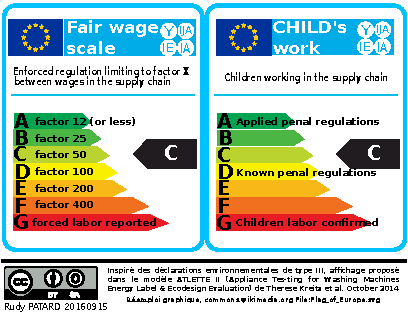
\includegraphics[width=\textwidth]{/home/rudy/Documents/rudy/01_These/11_production/01_COMMUNICATION/figures/declaration_soutenable_pdt_A.pdf}
   \caption{Visions alternatives de l’étiquetage environnemental et durable.
   Quelle information supplémentaire donner aux consommateurs pour guider leur choix~?
   Proposition basée sur ATLETE II~\cite{therese_kreitz_atlete_2014}}
   \label{fig:declaration_soutenable_pdt}
 \end{figure*}
   
 \figbox{
Dans la figure~\ref{fig:declaration_soutenable_pdt}, nous proposons des alternatives d'affichage hypothétiques sur la base du modèle ATLETTE II.
Partant de lidée d'illustration de la proposition initial des auteurs \citeauthor{therese_kreitz_atlete_2014}, sur une échelle de classe de consommation d'énergie, nous proposons des graphiques alternatifs.
L'illustration à gauche est une proposition basée sur l'écart salarial au sein de la chaîne de valeur.
L'illustration de droite propose l'affichage d'une échelle sur le travail des enfants dans la chaîne de fournisseurs.
}
\keybox{Nous le voyons donc, la reconnaissance de l'intérêt public dans l'accès à une information ou sa reconnaissance comme faisant partie du domaine privé conditionne la capacité à réaliser de l'ACV.
Ceci implique que tant qu'une information jugée privée\footnote{Dans les exemples il s'agit de la distribution des salaires et de l'âge dans la chaîne de valeur.} est nécessaire à l'ACV, un équivalent ouvert, mentionnant les écarts possibles et hypothèses attenantes doit être produit.}

  
\subparagraph{Exigences~:}
 \begin{itemize}[noitemsep,topsep=0pt,parsep=0pt,partopsep=0pt]
  \item Les orientations des licences sur les données et outils doivent libérer ces derniers des contraintes du droit d'auteur et de la propriété intellectuelle, justement pour ne pas les enfreindre.
  Pour toute donnée fermée l'équivalent ou substitut ouvert doit être produit avec la plus grande ouverture et transparence.
  Les licences employées doivent laisser un maximum de liberté à la création, modification, distribution des données, codes et résultats. 
  
  \item Le système doit lever toute limitation en terme de système de valeur. Ainsi, il doit gérer l'inconsistance \emph{au sein des} systèmes de valeurs et \emph{entre les} systèmes de valeurs, sans être une imposition de valeurs contraire à la réglementation.
  
  \item Le système doit protéger les déclarants sur l’énoncé de leurs jugements.\footnote{
  Lié à la question de la liberté d'opinion, de ton et de parole, au plan international, il s'agit d'un point sensible.
  Il doit être défini de façon claire sur les modalités de transparence et d'espace privé.
  Pour une personne morale, où considérons nous qu'une information privée portant sur des dangers pour d'autres, devrait ou non être révélée au public~?
  }.
 \end{itemize}
 
%
% Requirement:
% \begin{enumerate}[noitemsep,topsep=0pt,parsep=0pt,partopsep=0pt]
%  \item So the chosen regulation under which put the data and tools must be clearly selected toward this goal: free-open.
%  \item Allow no value system limitation.
%  So handle inconsistencies within value systems.
%  \item Protection on personal judgments declaration\footnote{It is linked to the theme of freedom of opinion and freedom of speech. Here must also be chosen the side between transparency and privacy. Where do we consider that private information but harmful to all should not be disclosed?}.
% \end{enumerate}
% 
\subparagraph{L'Observateur--trice~:}
\subparagraph{Description de l'inter-acteur~:}
 Avant même d'être utilisateur de l'\gls{ACV} ou de ses résultats, une personne peut être observatrice de l'outil.
 Il a été souligné au \ref{sec:La pensée en cycle de vie} que la question de la légitimité et de la confiance en l'\gls{ACV} est un point essentiel pour qu'elle soit considérée et employée (i.e. que des personnes deviennent utilisateur et décideur comme nous le verrons ensuite).
 Plus l'outil apparaîtra comme obscure, inconsistant, moins il apparaîtra comme sûr et digne d'intérêt.
 Pour qu'un observateur considère l'information fournie par l'\gls{ACV} comme valide, crédible et légitime, la méthode et son application doivent être transparentes. Ceci est nécessaire pour assurer la confiance de l'observateur dans la capacité d'une prise de décision au delà de nos limites cognitives actuelles, cf. sec~\ref{sec:ADMC}.
% L'\gls{ACV} doit gagner en légitimité et en crédibilité par plus de transparence et assurant la confiance dans la capacité d'une prise de décision au delà de nos limites actuelles~\ref{label}.

 En plus des outils et données ouvertes (spécifiés dans les exigences sur le système de données), apparaît ici la nécessité d'information complémentaire de vulgarisation.
 L'\gls{ACV} n'est pas limitée à ceux qui la pratiquent.
 Elle doit pouvoir, lorsqu'elle est observée, être comprise par ceux qui potentiellement et à des degrés divers la subissent. %garde-t-on subir ?
 
%\colorbox{yellow}{Trouver un // sur l'information du consommateur sur les subst.dangereuses.}
%
%\colorbox{yellow}{Confrontation du thème de la publicité et de l'information.}
%
%
%
%\colorbox{yellow}{obstacle à l'intervensionisme de l'utilisateur dans le système de valeur}
 \subparagraph{Exigences~:}
 \begin{itemize}
 \item Une vulgarisation progressive doit être disponible pour tout observateur.
 \item La \textbf{distinction} entre \textbf{faits} et \textbf{opinions} doit être \textbf{systématique} pour assurer la confiance au futur décideur potentiel dans l'application de \emph{son} système de valeur\footnote{Nous retrouvons des conséquences classiques en conception relative à `l'observateur', qui se résume à~: attirer l'utilisateur potentiel.}.
 \end{itemize}
 
 
 \subparagraph{L'Utilisateur--trice~:}
 \subparagraph{Description de l'inter-acteur~:}
 Ici, nous considérons l'utilisateur de l'\gls{ACV}.
 Il s'agit donc de l'entité qui modélise et qui calcule l'\gls{ACV}.
 Ceci peut être perçu comme le praticien (LCA practitionner).
 L'utilisateur de l'\gls{ACV} n'est pas nécessairement, le décideur.
 
 Il s'agit ici de prendre à contre-pied \emph{`l'impossible délégation'} de l'évaluation de \citeauthor{grahl_evaluation_1996} section \ref{grahl_impossible_deleguation}.\label{délégation de valeurs2}
 L'utilisateur doit produire un résultat dans un cadre décisionnel (comme vu section \ref{subsec:besoin}).
 S'il n'est pas possible de produire une évaluation sans le système de valeurs du décideur, il n'est pas interdit de faire appliquer ledit système par un tiers.
 \textit{De facto}, il s'agit donc d'une délégation de l'évaluation mais pas un changement de décideur.
 En effet, nous pouvons rendre possible la délégation de l'évaluation par la \emph{transmission du système de valeur du décideur à l'utilisateur}.
% Soit pour une décision directe, soit pour la fourniture d'une information exploitable lors d'une décision ultérieure\footnote{Distinction des cas de décision suivant l'ILCD, Table "Study types"\cite{european_commission_ilcd_2010}}.
 Le cadre méthodologique de l'\gls{ACV} doit donc permettre au praticien de s'extraire des jugements appliqués, sans ambiguïté.
 L'utilisateur devant répondre au décideur suivant son contexte de décision, la temporalité de l'évaluation ne doit pas dépasser celle de l'action de décision.
 Dans un temps limité, l'utilisateur doit donc produire une représentation compréhensible d'une préférence entre alternatives sur la base d'une grande étendue d'informations (bis repetita des arguments du point relatif au système d'information~\ref{subparagraph:Le Système d'information}). % centaines, miliers d'info (3000 substance, 8000 procédés, plusieurs dizaines d'indicateurs et leurs agrégations)
  \subparagraph{Exigences~:}
 \begin{itemize}[noitemsep,topsep=0pt,parsep=0pt,partopsep=0pt]
  \item L'\gls{ACV} doit présenter de façon lisible et compréhensible son processus et ses résultats.
  \item L'\gls{ACV} doit prendre en compte les limites cognitives humaines durant son processus et employer des méthodes et outils permettant de dépasser nos limites de rationalité.
%  \marginpar{? \textbf{Cosmin}, quelle contradiction}
  \item L'\gls{ACV} doit apporter une réponse pour la prise de décision dans le cadre temporel de la décision, \emph{sans y mêler le jugement de l'utilisateur} lorsque celui-ci diffère du décideur.
 \end{itemize}
% \item Observer:
% 
% Before using LCA or its resulting information, a person can observe LCA.
% It has been pointed out that LCA must earn its legitimacy to be considered a proper tool for decisions. (RETROUVER LA SOURCE)
% The more obscure or inconsistent, the less secure and interesting the tool appear.
% LCA must gain in legibility and transparency to secure trust and confidence in the decision it enables.
% 
% Requirement:
% 
% On top of open access to data and tools (specified with information system requirements), the information must be presented with force of vulgarization, consistence.
% The distinction between facts and opinion shall be systematic.
% 
% \item User:
% Here we specify a user of LCA.
% This entity is the one that models and calculates.
% It can be seen as the LCA practitioner.
% It is not (necessarily\footnote{
% Apart for those doing LCA for their own decision.
% A reality that could arise sooner than we anticipate.})
% the user of the result of LCA.
% 
% Requirement:
% \begin{enumerate}[noitemsep,topsep=0pt,parsep=0pt,partopsep=0pt]
%  \item The LCA must present human readable conclusion and process.
%  \item It must respect human cognitive limits or apply methods and other artifact to exceed them.
% \end{enumerate}


\subparagraph{Le Décideur~:}
\label{decideur}
 \subparagraph{Description de l'inter-acteur~:}
 \blockcquote[traduction]{murray_transdisciplinary_2015}{Les normes d'ACV identifient directement différents décideurs institutionnels, y compris l'industrie (développement de produits, le marketing, la planification stratégique) et le gouvernement (politique publique), mais les consommateurs et les citoyens ne sont pas directement mentionnés. En revanche, le consommateur est un centre d’attention d'une économie axée sur la demande et les préférences des consommateurs, des orientations et des visions du monde valeur informent des discussions LCA de valeurs (par exemple Hofstetter et al., 2000).}
% LCA standards directly identify various institutional decision makers including industry (product development, marketing, strategic planning) and government (public policy), but consumers and citizens are not directly mentioned. In contrast, the consumer is a focus of a demand-driven economy and the consumer’s preferences, value orientations and worldviews inform some LCA discussions of values (e.g. Hofstetter et al. 2000).
% }
 
   Le décideur (individu ou groupe) soumet son/ses systèmes de valeurs pour que la solution qui sera sélectionnée corresponde à ce système de valeurs.
   Qu'il(s) choisisse(nt) d'être en nombre limité (mona-oliga-rchie), ou de distribuer plus largement la déclaration de préférences,
   le décideur \emph{doit avoir la maîtrise du système de valeurs employé} dans cette expression de l'é\emph{valuation}.
   L'apport primordial du décideur à l'\gls{ACV} est le système de valeur.
   Il doit pouvoir se consacrer à son expression et faire que celle-ci soit la plus exploitable.
   En considérant que les valeurs d'un individu stable le sont également, le système de valeurs doit être applicable indépendamment du contexte (donc de l'application).
      
 \subparagraph{Exigences~:}
 
 L'\gls{ACV} doit permettre
 
 \begin{itemize}[noitemsep,topsep=0pt,parsep=0pt,partopsep=0pt]
  \item l'intégration du système de valeurs du décideur (individu ou groupe)~;
  \item le contrôle par le décideur de l'application de son système~;
  \item l'obtention d'une représentation de sa préférence envers les alternatives qui lui soit accessible (disponible et compréhensible)~;
  \item la protection du décideur dans sa déclaration d'opinions, \emph{si celle-ci doit pouvoir rester privée}~;
 \end{itemize}
% \item Stakeholders:
% 
% This category is large.
% We specified a user and an observer category for their specificities.
% Who are those concerned with the applications of LCA (``Product development and improvement, Strategic planning, Public policy making, Marketing, Other''\cite[Figure 1 Framework for life cycle assessment (from ISO 14040:2006; modified)]{european_commission_ilcd_2010})?
% I could discern two subcategories\footnote{These subcategories are not disjoint. But the range of consequences is not necessarily uniformly distributed among the discussed categories.}:
% \begin{itemize}[noitemsep,topsep=0pt,parsep=0pt,partopsep=0pt]
%  \item Decision maker(s) (causal party)
%  \item Decision affected parties (consequence party)
% \end{itemize}
% If we are to apply a tool with such an important impact in terms of application, we shall consider the political implication in terms of governance.
% The decision maker(s) submitting her/his/their value system for their preferred solution to be selected chose to either be in limited number (oligarchism) or to distribute the declaration of preferences.
% In a case where those suffering the negatively perceived consequences are not those beneficing the positively perceived ones debating who rightfully claim the preference system to be applied is of prime importance.
% This also imply that the communication of information must be done so that it reflect the decision maker(s) selection.
% For democratic context, a complete vulgarization and systematic progressive explanation is necessary.
% 
% Requirement: LCA must provide
% \begin{enumerate}[noitemsep,topsep=0pt,parsep=0pt,partopsep=0pt]
%  \item Consistence between political perspective(s) and implementation of value systems of stakeholders.
%  \item Wide sets of representations accessible (that can be reached and understood) to all stakeholders.
% \end{enumerate}
 
\subparagraph{Autres parties prenantes~:}
 \subparagraph{Description de l'inter-acteur~:}
 
%  C'est ici une large catégorie.
  Les utilisateurs, décideurs et observateurs sont spécifiés pour leurs particularités.
  Il convient maintenant également de traiter ceux qui seront concernés par l'application de l'\gls{ACV} (``Product development and improvement, Strategic planning, Public policy making, Marketing, Other''\cite[Figure 1 Framework for life cycle assessment (from ISO 14040:2006; modified)]{european_commission_ilcd_2010}), sans qu'ils fassent usage de l'\gls{ACV}, soient à l'origine du système de valeurs employé ou sans même  qu'ils observent l'un (le système de valeur) ou l'autre (l'\gls{ACV}).
  Deux sous-catégories de parties-prenantes sont discernées~:
  \begin{itemize}[noitemsep,topsep=0pt,parsep=0pt,partopsep=0pt]
   \item Décideur(s), (Decision maker(s)) (partie causale), traitée précédemment,
   \item Parties affectées (partie conséquence)
  \end{itemize}
  Ces sous-catégories ne sont pas disjointes.
  Mais la plage de conséquences n'est pas nécessairement uniformément distribuée sur ces catégories.
  Il peut être avancé qu'un décideur, ayant intégré une plus grande part d'information, notamment relative aux conséquences, puisse agir sur des décisions personnelles conduisant à une moindre exposition aux conséquences négatives et/ou à une plus grande exposition aux bénéfices des choix actés
  \footnote{Question du délit d'initié.}.
  Si nous appliquons un tel outil avec des conséquences importantes en termes d'applications (\textit{cf.} la section relative aux applications de l'\gls{ACV}~\ref{sec:La pensée en cycle de vie}), nous devons prendre en compte les \emph{implications politiques en terme de gouvernance}.
   
  Dans un cas où ceux subissant les conséquences perçues négativement ne sont pas ceux bénéficiant des conséquences perçues positivement, débattre de qui peut légitimement déterminer quel système de valeurs sera appliqué est de première importance.
  Ceci implique également, en termes de communication, que le message (s'il en est un de diffusé) doit inclure la façon dont a été déterminé le \emph{système de valeurs décisionnaire} (la sélection du décideur).
  \exbox{
  Pour reprendre notre exemple de l'affichage environnemental (figure \ref{fig:declaration_soutenable_pdt}), celui-ci devrait donc porter une explication du système de valeur employée. Exemple, une mention du type : panel européen à intervalle de confiance de 95\%
%  \marginpar{\textbf{voir Cosmin}}
%  \marginpar{"Il porte déjà (parfois)"}
  adjoint à une localisation pour l'accès et l'observation de ce système de valeur (ex~: une URL).
  }
  Une partie prenante par voie de conséquence doit pouvoir devenir observatrice sous les gouvernements qui en juge ainsi de l'information des citoyens.
  
  Dès-lors qu'une partie prenante peut introduire son propre système de valeur en substitution de celui employé pour l'évaluation, elle devient le décideur.
  \exbox{
  ex: hypothèse du développement d'une application, soit mobile par QR-code, soit sur ordinateur pour le e-commerce, qui reproduit l'affichage suivant le système de valeur du consommateur).}
  Les exigence de ce groupe s'appliquent alors cf. (\ref{decideur}) inter-acteur précédent.
  \subparagraph{Exigences~:}
  
  L'\gls{ACV} doit fournir~:
  
  \begin{itemize}[noitemsep,topsep=0pt,parsep=0pt,partopsep=0pt]
   \item une \textbf{consistance} entre le cadre politique et l'implémentation des systèmes de valeurs des parties prenantes\footnote{Ex~: Une décision publique dans un cadre démocratique emploie le système de valeurs du peuple auquel s'applique la décision.}~;
   \item une large gamme de représentations du système de valeurs appliqué, accessible à l'\emph{ensemble} des parties prenantes, accessible dans ses deux acceptions, qui peut être \emph{atteinte} et \emph{comprise}.
  \end{itemize}
  


\paragraph{Caractérisation des Fonctions de Service (F.S.)}

%\paragraph{Synthèse des exigences fonctionnelles}
Reprenant les interacteurs, nous identifions un certain nombre de fonctions récurrentes, issues des exigences.
À la suite de plusieurs itérations de reformulation des exigences, nous obtenons une liste réduite de fonctions de services. %, principale et contraintes (en réponse au besoin extérieur et imposées par l'environnement pour obtenir le service).
%\marginpar{\textbf{Cosmin}{\tiny J'ai repris les brouillons pour écrire les tables de reformulation. Mais même en annexe je ne trouve pas qu'elles aient leur place}.}
L'objectif de la première phase de cette étape est d'obtenir la liste minimale des fonctions à caractériser.
Cette liste est reprise table~\ref{tab:ACV-fonctions}.


%\begin{longtable}{p{2.5cm}|p{2cm}|p{8cm}}
%inter-acteur & libellée & fonction \\
%\hline
%
%Le système d'information & FC1 & L'ACV doit être adapté aux écarts linguistiques et culturels.\\
%Le système d'information & FC2 & L'ACV doit permettre le traitement de multiples ontologies.\\
%Le système d'information & FC3 & L'ACV ne doit pas comporter de barrières ou couloirs d'étranglement à la mise à jour et à la correction.\\
%Le système d'information & FC4 & L'ACV doit s'inscrire dans les versions des observations.\\
%Le système d'information & FC5 (FC1' FC2') & L'ACV doit être développée avec de multiples standard de communication.\\
%Le système d'information & FC6 & L'ACV doit être accessible et fourni à travers le globe et éditable depuis chaque localité.\\
%Le système d'information & FC7 & L'ACV et son contenu doivent être lisibles par machine.\\
%Le système d'information & FC8 & L'ACV doit contenir à la fois les descriptions objectives et les valeurs et opinions.\\
%Le système d'information & FC9 & L'ACV doit permettre une distinction claire des deux natures d'information stockées~: objectif et subjectif.\\
%
%Réglementation & FC10 (FC3') & L'ACV doit reposer sur des licences permettant librement la modification, l'utilisation, transmission.\\
%Réglementation & FC11 (FC1') & L'ACV doit lever toute limitation en terme de système de valeur.\\
%Réglementation & FC12 (FC2') & L'ACV doit gérer l'inconsistance au sein des systèmes de valeurs et entre les systèmes de valeurs.\\
%Réglementation & FC13  & L'ACV doit employer un système d'information qui protège les déclarants sur l’énoncé de leurs jugement.\\
%  
%Observateur& FC14 (FC1') & L'ACV doit comporter une vulgarisation progressive et disponible à tout observateur (FC1-FC2).\\
%Observateur& FC15 & L'ACV doit assurer sa propre crédibilité.\\
%Observateur& FC16 (FC9') & L'ACV doit permettre la distinction systématique entre faits et opinions. RQ : moyen à FC15.\\
%
%Utilisateur& FP1 & L'ACV doit présenter de façon (lisible et compréhensible : FC17), la préférence du décideur envers une série d'alternatives, suivant la globalité de son système de valeurs.\\
%Utilisateur& FC17  & L'ACV doit respecter les limites cognitives humaines durant son processus et employer des méthodes et outils permettant de dépasser ces limites de rationalité.\\
%Utilisateur& FP2 (FP1') & L'ACV doit respecter le cadre temporel de la prise de décision de l'utilisateur.\\
%
%Parties prenantes & FC18 &  L'ACV doit fournir une consistance entre le cadre politique et l'implémentation des systèmes de valeurs des parties prenantes.\\
%Parties prenantes & FC19 (FC6')(FC6' FC14' FC1') &  L'ACV doit fournir une large gamme de représentations accessible (dans ses deux acceptions, qui peu être atteinte et comprise) et cela à l'ensemble des parties prenantes.\\
%\end{longtable}
%
%
%\begin{longtable}{p{2.5cm}|p{2cm}|p{8cm}}
%inter-acteur & libellée & fonction \\
%\hline
%
%Le système d'information & FC1 & L'ACV doit être adapté aux écarts linguistiques et culturels.\\
%Le système d'information & FC2 (FC1') & L'ACV doit permettre le traitement de multiples ontologies.\\
%Le système d'information & FC3 & L'ACV ne doit pas comporter de barrières ou couloirs d'étranglement à la mise à jour et à la correction.\\
%Le système d'information & FC4 & L'ACV doit s'inscrire dans les versions des observations.\\
%Le système d'information & FC6 & L'ACV doit être accessible et fourni à travers le globe et éditable depuis chaque localité.\\
%Le système d'information & FC7 (Moyen FC17') & L'ACV et son contenu doivent être lisibles par machine.\\
%Le système d'information & FC8 (Moyen FP1)& L'ACV doit contenir à la fois les descriptions objectives et les valeurs et opinions.\\
%Le système d'information & FC9 & L'ACV doit permettre une distinction claire des deux natures d'information stockées~: objectif et subjectif.\\
%
%Réglementation & FC10 & L'ACV doit suivre un développement qui limite les contraintes réglementaires s'imposant à elle.\\
%Réglementation & FC13 & L'ACV doit protéger les déclarants sur l’énoncé de leurs jugements, avant et après cet énoncé.\\
%  
%Observateur& FC14 (FC1') & L'ACV doit comporter une vulgarisation progressive et disponible à tout observateur (FC1-FC2).\\
%Observateur& FC15 & L'ACV doit assurer sa propre crédibilité.\\
%Observateur& FC16 (FC9') & L'ACV doit permettre la distinction systématique entre faits et opinions. RQ : moyen à FC15.\\
%
%Utilisateur& FP1 & L'ACV doit présenter de façon (lisible et compréhensible : FC17), la préférence du décideur envers une série d'alternatives, suivant la globalité de son système de valeurs.\\
%Utilisateur& FC17  & L'ACV doit respecter les limites cognitives humaines durant son processus et employer des méthodes et outils permettant de dépasser ces limites de rationalité.\\
%Utilisateur& FP2 (FP1') & L'ACV doit respecter le cadre temporel de la prise de décision de l'utilisateur.\\
%
%Parties prenantes & FC18 (FP1') &  L'ACV doit fournir une consistance entre le cadre politique et l'implémentation des systèmes de valeurs des parties prenantes.\\
%Parties prenantes & FC19 (FC6' FC14' FC1') &  L'ACV doit fournir une large gamme de représentations accessible (dans ses deux acceptions, qui peu être atteinte et comprise) et cela à l'ensemble des parties prenantes.\\
%\end{longtable}

%itération 3 -> reformulation et agrégation
%>> reformulation encours avec les graphes
%


%\begin{longtable}{p{2.5cm}|p{2cm}|p{8cm}}
%libellé initiaux & renumérotation & fonction \\
%\hline
%FP1 & FP1 & L'ACV doit présenter la préférence du décideur envers une série d'alternatives, suivant la globalité de son système de valeurs.\\
%FC17 & FC1 & L'ACV doit respecter les limites cognitives humaines durant son processus et permettre de les dépasser.\\
%%FC8 & FC2 & L'ACV doit contenir à la fois les descriptions objectives et les valeurs et opinions.\\
%FC1 & FC2 & L'ACV doit être adaptée aux distributions géographiques, linguistiques et culturels des parties prenantes.\\
%FC3 & FC3 & L'ACV doit assurer son développement en données.\\
%FC15 & FC4 & L'ACV doit assurer sa validité et crédibilité.\\
%FC10 & FC5 & L'ACV doit suivre un développement qui limite les contraintes réglementaires s'imposant à elle.\\
%FC13 & FC6 & L'ACV doit protéger les déclarants sur l’énoncé de leurs jugements, avant et après cet énoncé.\\
%\end{longtable}

\begin{table}[h]
\begin{tabular}{p{2cm}|p{10cm}}
Libellé & fonction \\
\hline
FS1 & \textbf{Présenter la préférence du décideur} envers une série d'alternatives, suivant la globalité de son système de valeurs.\\
FS2 & \textbf{Respecter les limites cognitives} humaines.\\
FS3 & \textbf{Être adaptée aux distributions culturels}.\\
FS4 & \textbf{Assurer son développement en données}.\\
FS5 & \textbf{Être valide et crédible}.\\
FS6 & \textbf{Respecter les contraintes réglementaires}.\\
FS7 & \textbf{Protéger les déclarants} sur l’énoncé de leurs jugements.\\
\end{tabular}
\caption{Fonctions de l'\gls{ACV}}
\label{tab:ACV-fonctions}
\end{table}



%\colorbox{yellow}{MAJ de la figure avec les nouvelles descriptions de fonction}
%
%\colorbox{yellow}{écart entre \ref{fig:octopus_LCA} et \ref{fig:interacteurs et fonctions}.}


%\begin{figure}[htbp]
%  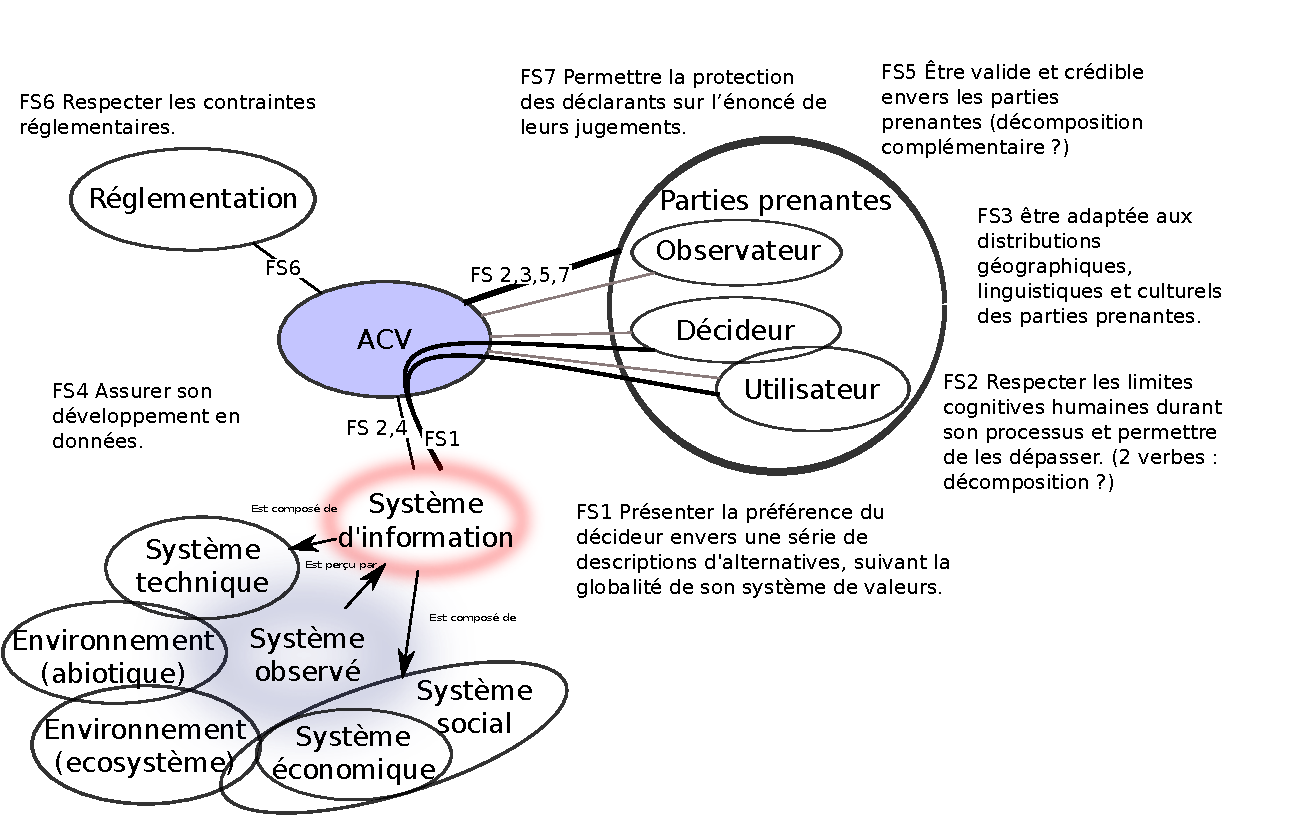
\includegraphics[width=1\textwidth]{/home/rudy/Documents/rudy/01_These/11_production/01_COMMUNICATION/figures/octopus_ACV-ref-fonction.pdf}
%  \caption{Représentation des fonctions sur la graphe des interacteurs. }
%  \label{fig:interacteurs et fonctions}
%\end{figure}
\begin{figure}[htbp]
  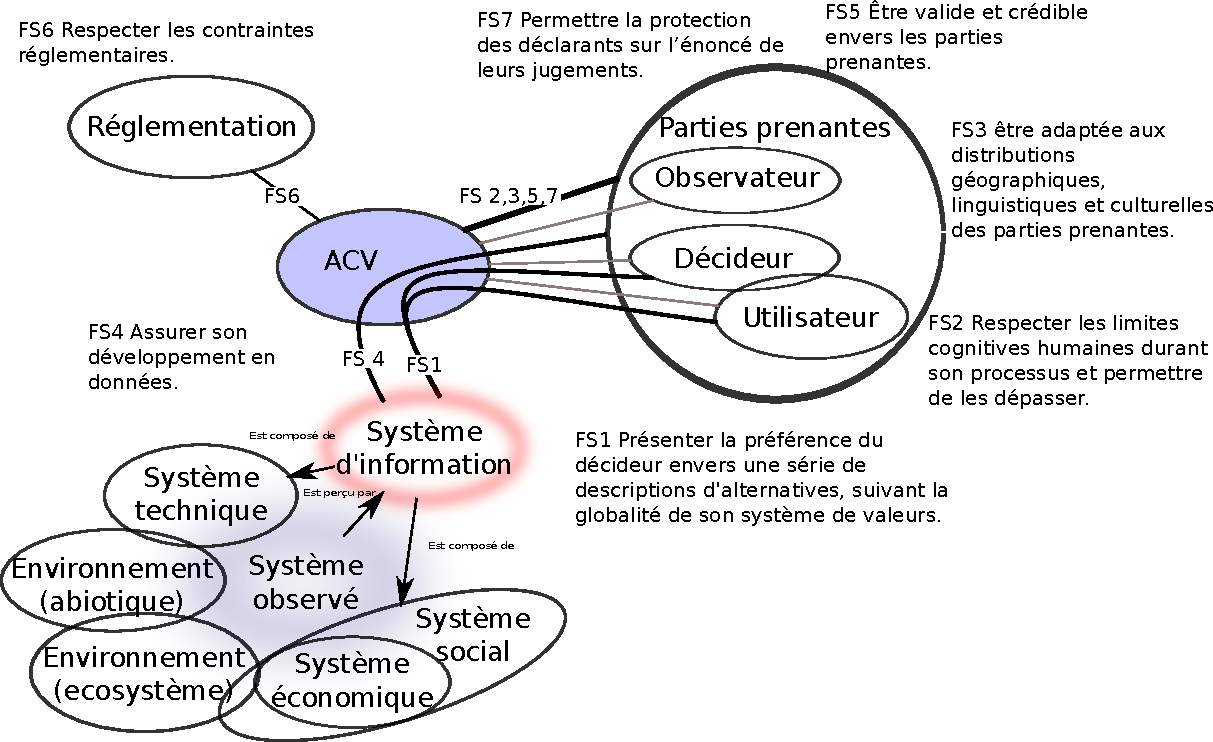
\includegraphics[width=1\textwidth]{/home/rudy/Documents/rudy/01_These/11_production/01_COMMUNICATION/figures/octopus_ACV-ref-fonction_V2.pdf}
  \caption{Représentation des fonctions sur la graphe des interacteurs. }
  \label{fig:interacteurs et fonctions}
\end{figure}
\figbox{
La représentation finale des interactions est donnée figure~\ref{fig:interacteurs et fonctions}.                  
En représentation de diagramme des intéracteurs, les fonctions contraintes sont des traits simples liant \textbf{un} EME au produit.
Les fonctions 'principales' sont représentées par des traits courbes, liant à minima \textbf{deux} EME au produit.

Nous observons qu'une série de contraintes identiques (2,3,5,7) s'appliquent à l'ensemble des parties prenantes, qu'elles soient conservées intégralement ou non dans le groupe 'décideur'.

L'évaluation ne peut pas être faite sans l'interaction du décideur.
Elle peut toutefois être réalisé par l'utilisateur après transmission du système de valeurs du décideur.
Ceci est représenté par le trait courbe en fourche (Système d'information, décideur, utilisateur) signifiant la première fonction de service (FS~1).
}

\subparagraph{Discussion} sur la distinction entre fonctions contraintes et fonctions principales.

La fonction FS~4 met en interaction des parties prenantes et le système d'information au travers l'\gls{ACV}.
Les données d'observations peuvent être d'origine variées (non nécessairement des données d'inventaires spécifiques pour l'\gls{ACV}).
Les données sont produites par des tiers et donc des 'parties prenantes' productrices de données employées en \gls{ACV} contribuent au système d'information (FS~4).
Toutefois des données peuvent ne pas correspondre à ce qui est exploitable dans les méthodes d'impacts. % (\textit{cf.} \ref{} couverture et spécificité de la données).
Il doit donc y avoir des 'ponts de langage' entre les données des parties prenantes hors \gls{ACV} et les méthodes d'impacts (données sur les mécanismes environnementaux).
Définir FS~4 en contrainte ou principale réside dans la distinction entre~:
\begin{itemize}
\item L'\gls{ACV} doit \textbf{exploiter} les croisements d'ontologies \emph{existants} (contrainte du système d'information vers l'\gls{ACV}).
\item L'\gls{ACV} doit \textbf{développer} les croisements d'ontologies des \emph{existantes} (principale~: construction avec les parties prenantes d'éléments de langages communs).
\end{itemize}
Notre perception de l'\gls{ACV} par sa pratique nous pousse à retenir la seconde déclaration.
%\paragraph{Caractérisation des Fonctions de Service}

La distinction entre fonction contrainte et principale nous parait dans d'autre cas moins applicable et exploitable.
Certains cas complexes rendraient les représentations peu exploitables par un grand nombre de ligne courbe perdant le lecteur.
Par exemple, les fonctions FS~2,3,5,7 portent toutes sur l'ensemble des parties prenantes.
Mais elles peuvent très bien être lu comme des liaisons entre plusieurs EME.
Si la FS~7 vise la protection des déclarants (i.e. décideur), elle les protège des autres parties prenantes et reste pour l'observateur une source de confiance dans un futur potentiel emploi de l'\gls{ACV}.
FS~7 se mêle alors à la validité et la crédibilité de la démarche (FS~5-7).
Cette protection peut également s'appuyer de la législation qui s'y rapporte (FS~7-6).
Des clauses particulières peuvent encadrer la relation entre l'utilisateur et le décideurs

La production de confiance (validité, crédibilité, FS5) peut porter (i) du décideur pour lui-même (ii) du décideur vers l'observateur lors d'une décision publique (iii) ou encore de l'utilisateur vers le décideur et/ou l'observateur pour s'assurer de sa non-interférence.

Plutôt que d'alourdir inutilement la figure~\ref{fig:interacteurs et fonctions}, ou de la déclinée dans de multiples versions, nous passons de l'identification à la caractérisation.

\subparagraph{Tables de caractérisation.}
Les tables de caractérisation définissent les modalités selon lesquelles le produit répondra aux fonctions.
Les champs traditionnellement employés sont le libellé de la fonction, les critères observés (entité quantifiée ou qualifiée), le niveau (quantification ou qualification cible), la flexibilité\footnote{Afnor FD X 50-159, fiche O5 "caractériser les fonctions"}.
Nous n'irons pas jusqu'à nous permettre de définir la flexibilité avec laquelle nous souhaitons voir l'\gls{ACV} révisée.
De même nous ne hiérarchisons pas les fonctions entre-elles.
Le but de cette exercice n'est pas tant de donner un cahier des charges pour l'\gls{ACV} mais d'identifier les fonctions de services manquantes à l'état actuel de la méthodologie pour corriger celle-ci.
Nous suggérerons toutefois un certain nombre de critères et de niveaux dans la table~\ref{tab:carac-ACV-fonctions}, sur la base de l'argumentaire développé ci-dessous pour chaque fonction.
%? Niveau Flexibilité  > discussion uniquement des Critères ? proposition de niveau ?

\subparagraph{FS1~:~Présenter la préférence du décideur.}
Il nous semble évident que, si la finalité de l'objet à concevoir et d'appliquer un jugement de valeur à des observations, le jugement de valeur comme les descriptions doivent être respectés.
c.a.d que~:
\begin{itemize}
\item la globalité du jugement doit être employé (pas d'heuristique, 100~\% du jugement émit).
\item toute description utile doit être exploitée (pas de coupure \textit{a~priori}, 100~\% de l'information disponible).
\end{itemize} 
L'implication d'un délai à la restitution de l'évaluation vise encore une fois à marquer l'intégration à un processus de décision.
Suivant chaque contexte décisionnel, il peut s'agir de l'ordre de l'heure (panier d'achat web), de jours (réponse à des fournisseurs) voir de mois ou des années (études de décisions stratégiques, ex: nations, multi-nationales).

\subparagraph{FS2~:~Respecter les limites cognitives}
Les limites cognitives, en termes de nombre d'objets à conserver en mémoire de travail, sont basses (moins de 7 pièces d'information nouvelles et potentiellement jusqu'à seulement 3)~\cite{farrington_seven_2011}.
Il convient donc de limiter ce nombre d'éléments à mémoriser afin de rendre la procédure la plus accessible possible.
Par ailleurs, il n'est pas possible de limiter les dimensions observées (indicateurs), sans faire obstacle à la diversité culturelle potentielle (FS3).
Il ne doit donc pas y avoir de limite théorique que ce soit sur les dimensions observées ou sur les alternatives considérées.

De plus, dans son expression complète nous spécifions pour cette fonction "Respecter les limites cognitives humaine et permettre de dépasser nos limites de rationalité".
En effet pour valider les critères et niveau de FS1 (emploi de la globalité du jugement et des descriptions du système observé), tout en restant sous le seuil de surcharge cognitive, il convient d'attester de la rationalité du jugement mis en œuvre (de sa consistance) et de valider celle-ci comme recevable.
Soit nous posons un seuil de consistance, soit nous considérons l'extraction de la part consistante du jugement~\cite{barzilai_consistency_1998}.
%\footnote{
Ce qui est perturbant dans l'\emph{extraction d'un jugement consistant} d'un jugement inconsistant, c'est qu'il ne peut s'agir \emph{que} d'une déformation du jugement exprimé.
Et sans savoir si cette extraction tend vers le jugement effectif du décideur ou si elle tend vers une meilleur accommodation d'une erreur d'expression du jugement, cela nous parait compliqué de réaliser cette extraction pour un individu unique.
Cette démarche nous semble toutefois parfaitement cohérente avec une logique de décideur multiple (groupe).
Dans ce cas en effet, le jugement du groupe étant une construction, donner l'aval à la partie commune et consistante du jugement d'un groupe semble parfaitement approprié.
%}
\subparagraph{FS3~:~Être adaptée aux distributions culturelles}

Plutôt que d'indiquer langage écrits, nous avons préféré langage 'transcriptible'.
Écrit serait un caractère plus excluant.
Toutefois toute culture non-écrite n'est pas nécessairement transcriptible.
Pour des questions de traçabilité, de capacité de vérification, nous nous limitons cependant aux éléments pouvant laisser une trace écrite.
 %, pouvant être transcrit.
 
Par ailleurs, les décideurs souhaitant intégrer les jugements des parties affectées sur les localisations d'impacts doivent pouvoir intégrer les jugements qui émanent desdites localités.
Il faut noter que ce type de processus nécessitera des déclarations particulières de la part de ces décideurs particuliers pour résoudre les inconsistances potentielles entre le système de valeurs adjoint et le leur.
Il faudrait en effet pouvoir résoudre spatialement l'inconsistance.
Si ce type de cas n'a sans doute pas d'importance pour la décision de personnes physiques, ceci semble capital pour des personnes morales d'envergure internationale (des états et leurs diverses unions, les multi-nationales).

\subparagraph{FS4~:~Assurer son développement en données.}
Comme cela aura été constaté à la sous-section correspondante~\ref{subsubsec:Bases de données}, bien que la qualité et l'accessibilité des données soit le thème récurent des problématique d'\gls{ACV} (cf~\ref{subsec:Problèmes méthodologiques}), le modèle organisationnel choisi jusqu'ici n'offre pas le service requis (nous manquons toujours largement de données).
Pour répondre à la fois à la problématique de responsabilité de l'auteur et d'une plus grande liberté dans l'élaboration et l'utilisation des données, nous considérons l'emploi de licence du \emph{type} CC-BY-SA (créative commons - attribution créditant l'auteur - partage dans les mêmes conditions), comme vu dans l'illustration~\ref{fig:AAA-FR}.

Une fois libéré des contraintes légales et réglementaires par ce choix organisationnel, c'est une caractérisation sur l'échelle du volume à traiter qu'il faut prévoir.
En complément de la mention présente pour FS~1 (exploitation de la totalité des descriptions disponibles), c'est une disposition rendant réalisable cette exploitation qui est nécessaire (la lisibilité par machine).

\subparagraph{FS5~:~Être valide et crédible.}
La validité et la crédibilité d'un outil d'aide à la décision sont des caractéristiques cruciales pour qu'il soit employé.
Sauf à reproduire à l'identique les mécanismes de confiances actuels, classiques, de la publication scientifique en recherche, il ne nous reste plus qu'à ouvrir les comités de revue et les mécanismes de révision eux-même.
Puisque la confiance \textit{hors de la capacité de vérification} tient à celui à qui on l'accorde, les données ne peuvent être inscrites anonymement.
Ceci sera développé au chapitre~\ref{chap:Recherche Libre}.
\subparagraph{FS6~:~Respecter les contraintes réglementaires.}
Nous posons comme évidence le fait de respecter la législation. Pour que l'ACV puisse être applicable, c'est la démarche \textit{active} de placer l'objet hors du champ des contraintes réglementaires qu'il convient d'acter.

Une partie du travail législatif actuel réside dans des accords pour faire sortir d'un domaine propriétaire des travaux des puissances publiques\footnote{À titre d'exemple citons le travail de \textsc{Couperin} sur la \href{https://www.republique-numerique.fr/consultations/projet-de-loi-numerique/consultation/consultation/opinions/section-2-travaux-de-recherche-et-de-statistique/exception-de-fouille-de-texte-et-de-donnees}{fouille de texte}.}.
Afin d'éviter tout obstacle qui rendrait la donnée caduque, obstacles de propriété lucrative notamment (et les diverses formes de propriété intellectuelle qui en sont les instruments), c'est le domaine \emph{libre de droit} qu'il convient de choisir nativement pour les données issue du travail public\footnote{Des travaux tels que ceux sur le génome humain, nous indiquent la voie depuis plus de vingt ans~\cite{pietu_projet_2013}}.
\subparagraph{FS7~:~Protéger les déclarants.}
Comme cela a été souligné à plusieurs reprise déjà, l'\gls{ACV} requière la déclaration d'un jugement de valeur.
L'espace de description objectif étant très vaste, il semble inadéquat de l'envisager hors ligne sauf pour des entreprises disposant de moyens considérables.
Le jugement va donc probablement être appliqué à de la donnée en ligne.
Il convient donc de protéger le déclarant.
Nous envisageons donc que les requêtes au système d'information de l'\gls{ACV} soient réalisées via un réseau d'anonymisation (ex: The Onion Router, TOR \cite{dingledine_tor:_2004,reed_anonymous_1998}).

%\colorbox{yellow}{introduction et conclusion après le tableau qui sont importante}
\subparagraph{Synthèse.}
Comme il est d'usage, nous synthétisons ces éléments dans une table de caractérisation.
Le tableau~\ref{tab:carac-ACV-fonctions}
\begin{table}
\begin{tabular}{p{5cm}|p{4.5cm}|p{4.5cm}}
\textbf{Fonction} & \textbf{Critère} & \textbf{Niveau}\\
\hline
%&&\\
\multirow{4}{*}{\parbox{5cm}{FS1 Présenter la préférence du décideur}} %envers une série d'alternatives, suivant la globalité de son système de valeurs.}}
	& Conformité au jugement du décideur & Identique au jugement émis\\ %\hline
	\cline{2-3}
	& Étendu des descriptions employer & 100\% \\ %\hline
	\cline{2-3}
	& Délai & (suivant cadre décisionnel)\\
%	&&\\
	\hline
\multirow{4}{*}{\parbox{5cm}{FS2 Respecter les limites cognitives humaines}}
	& Nombre d'éléments en mémoire & 3~\cite{farrington_seven_2011} \\ %\hline
		\cline{2-3}
	& Nombre de dimensions considérées & sans limite \\ %\hline
		\cline{2-3}
	& Nombre d'alternatives considérées	 & sans limite \\ %\hline
		\cline{2-3}
	& Seuil d'inconsistance	 & $CR < 0.1$ pour les individus~\cite{saaty_decision_2004}, inconsistance nulle pour les groupes\cite{barzilai_consistency_1998,ishizaka_how_2006}.\\ %\hline
\hline
\multirow{1}{*}{\parbox{5cm}{FS3 Être adaptée aux distributions culturels}}
	& Types de langage considérés & "transcriptible" \\
	&&\\
	\hline
\multirow{5}{*}{\parbox{5cm}{FS4 Assurer son développement en données}}
	& Étendue de la couverture	& Globale\\
		\cline{2-3}
	& Contrainte à la lecture	& Aucune hors infrastructure matérielle\\
		\cline{2-3}
	& Contrainte à l'écriture	& Aucune hors infrastructure matérielle\\
		\cline{2-3}
	& Contrainte à l'utilisation	& Aucune hors infrastructure matérielle\\
		\cline{2-3}
	& Lisibilité machine	& Pour toute donnée quantifiée ou qualifiée\\
	\hline
\multirow{3}{*}{\parbox{5cm}{FS5 Être valide et crédible}}
	& Nombre de revues critiques par donnée	& $\geq3$ ; selon système de valeurs du décideur*\\
			\cline{2-3}
	& Couverture de la revue	& Pluri-nationale ; *IDEM\\
			\cline{2-3}
	& Données Anonymes	& Non\\
	\hline
\multirow{1}{*}{\parbox{5cm}{FS6 Respecter les contraintes réglementaires}}
    & /	& /\\
	&	& \\
%	&	& \\
	\hline
\multirow{3}{*}{\parbox{5cm}{FS7 Protéger les déclarants}} % sur l'énoncé de leurs jugements.}}
	& Utilisation individuelle	& Via réseau de type TOR\\
				\cline{2-3}
	& Dépôt par un tiers pour les outils en lignes	& Systématique\\
				\cline{2-3}
	& Contrôle de la CNIL sur les dépôts	& Systématique\\
	\hline
\end{tabular}
\caption{Ébauche de caractérisation des fonctions de l'\gls{ACV}}
\label{tab:carac-ACV-fonctions}
\end{table}

\subsubsection{Analyse Fonctionnelle Technique}

L'exploration de l'espace des solutions répondant aux fonctions de service peut se faire au travers des diagrammes FAST (Function Analysis System Technique).

Ces diagrammes ont été produits fonction par fonction, tel que présenté en annexe \ref{subsec:FAST}.
Coupant avec les représentations classiques, fonction par fonction, sont représentés ici l'ensemble des éléments de la table~\ref{tab:ACV-fonctions} pour faire ressortir des réponses techniques \emph{communes} aux fonctions de services.

\begin{figure}[htbp]
  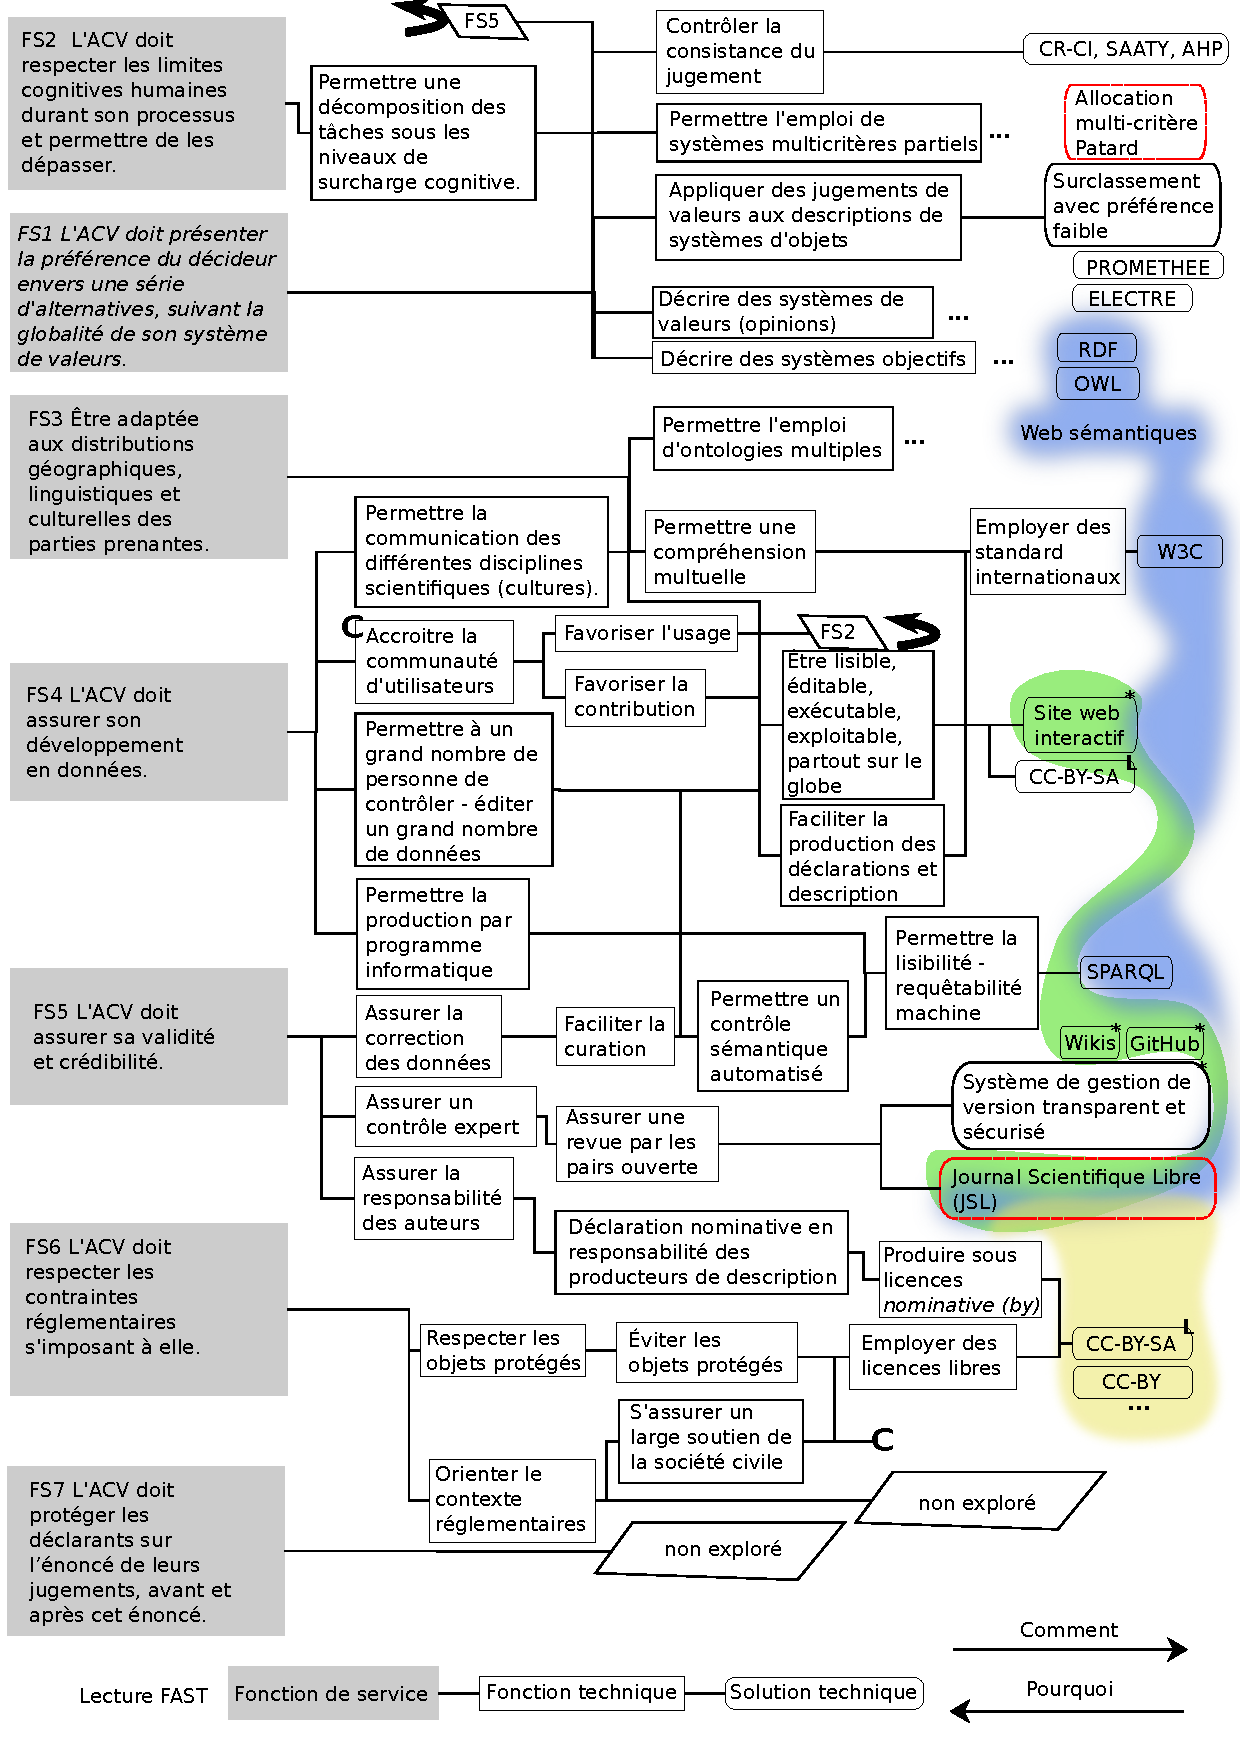
\includegraphics[width=\textwidth]{/home/rudy/Documents/rudy/01_These/11_production/01_COMMUNICATION/figures/FAST-fr_C.pdf}
  \caption{FAST}
  \label{fig:FAST_remix}
\end{figure}
\figbox{
Il apparaît lors de cette exploration des FAST combinés figure~\ref{fig:FAST_remix}, que des fonctions techniques sont communes à plusieurs fonctions de service.
Pour limiter le chargement de la figure de multiples traits additionnels et ne respectant pas les sens de lecture d'un diagramme FAST, nous procédons à des renvois par symbole.
\exbox{ex: ``S'assurer un large soutien de la société civile.'' \textsc{Comment}~?~: \textbf{C}, ``Accroître la communauté d'utilisateurs.''\ldots
``Contrôler la consistance du jugement'' \textsc{Pourquoi}~?~: ``FS5 L'ACV doit assurer sa validité et crédibilité.''\ldots}
En conséquence des solutions 'techniques' répondent à plusieurs fonctions.
Par exemple, le choix d'un système ouvert, transparent, avec gestion des versions et libre de droit, répond à de nombreuses contraintes sur l'adaptation aux parties prenantes, à la confiances pour celles-ci envers l'\gls{ACV} et dans le développement des données qui lui sont nécessaires (FS3 à FS6).

La question de la prise en compte des parties prenantes (en son sens le plus large FS1-3), tout en garantissant la protection des déclarants sur leur systèmes de valeurs (FS7) reprend des problématiques du vote électronique~\cite{enguehard_vote_2007,pellegrini_chaines_2014}.
Rappelons qu'il ne peut à la fois être garanti, que l'expression du jugement soit prise en compte \emph{et} que les expressions de jugements employées soient anonymes.
Il faut un procès de confiance.
Le recueil, pour les personnes souhaitant rester anonymes doit pouvoir être entré au système d'information par un tiers identifié et responsable de l'entrée de ces données nouvelles.
Sur un nombre vaste de dimensions, avec un nombre de combinaisons (valeurs de la matrice de jugement) d'importance relatives fortement supérieur au nombre de déclarant d'un groupe, il nous apparaît comme probable qu'un répondant puisse s'identifier au sein des systèmes de valeurs.
Ce point étant fortement éloigné de notre thématique initiale et de nos compétences, le soin en est laissé aux spécialistes de le poursuivre (Non-exploré).

Des évolutions législatives encours porte sur l'adaptation des administrations et de la gestion de données à l'ère des 'TIC' (République Numérique)~\cite{_republique_2015}.
Les délais d'embargo uniformisés entérinés par ce texte (bien que plus courts que ceux antérieurs~\cite{gouzi_loi_2016}), rendent délicat l'emploi d'une partie des données "fraîches" employables dans la part descriptives des systèmes observés.
Notamment sur les questions sociales où l'embargo est le plus long (12 mois), la nature des situations peut évoluer rapidement.
Par ailleurs, ces délais font obstacle à une procédure de vérification ouverte, repoussant encore le délai pour l'obtention d'une donnée validée ouvertement et par des pairs.
Une des orientations possibles pour certaines données de l'\gls{ACV} et le travail sous l'angle de l'exception de la recherche dans le domaine de la propriété (ex : exception pédagogique et de recherche~\cite{_droit_????}).
Elle se heurte toutefois à la multiplicité des législations et accords.
Or pour la recherche publique la voie reste libre à la libre publication comme développée au~\ref{sec:JSL}.
Une solution qu'il paraîtrait plus qu'inconsistant de la part de la recherche publique de ne pas employer.

Nous opérons la liaison des solutions de FS~1 ; FS~3-6 dans le journal scientifique libre, présentée au \ref{sec:JSL}.

}

À ce stade, si nous observons les fonctions requises, des solutions existantes apparaissent en littérature.


%For the respective requirement analysis,
%\begin{itemize}
% \item Application for decision,
% \item Dealing with multiple incommensurable attributes,
% \item Data intensive field, with data quality issues and continuous updates needed,
% \item Complex system representation that overwhelm individual human capacities.
%\end{itemize}
%
%
%PREFERENCE
%
%~\cite{these ADLA}
%~\cite{davis_making_2012}
%~\cite{sayan}
%~\cite{moullec_towards_2014}
%> clear depictions of MCDA as handling preferences. generally citing Roy and Bouyssou.
%The preference system being formalized around a limited set of criterionst}
%{Fonction de service}
%       \FT{FT1}
%       {
%         \FT{FT2}
%         {
%           \ST{Solution technique}
%         }
%       }
%       \FT{}
%       {
%         \FT{FT3}
%         {
%           \ST{ST2}
%         }
%       }
%       \FT{FT4}
%       {
%         \ST{ST3}
%       }
%{Fonction de service}
%       \FT{FT4}
%       {
%         \ST{ST3}
%       }
%       
%\end{fast}
%\fastReset
%
%This is what can be seen trough Rowley's work~\cite{rowley_aggregating_2012} as methods ``synthesising preference relational system'', in the classification of non-compensatory decision system, type 2 partial aggregation.
%
%Elements known before publication of ISO LCA standards: Roy, B., 1991. The outranking approach and the foundations of electre methods.
%Theory and Decision 31, 49e73.
%
%In literature we can find in isolation the different solutions.
%pass to table format
% \usepackage{multirow}

% \begin{landscape}
% \begin{table}[htbp]
%   \begin{center}
%   \caption{Characterization based on AF attributes Function, Criterion, Level, and current state in standard and practice.}
%   \begin{tabular}{|p{4cm}|p{4cm}|p{4cm}|p{3cm}|p{3cm}|}
%   \hline
%   Function&Criteria&Levels&Current state&Comments \\
%   \hline
%   \multirow{4}{*}{Enable the decision maker to select the option preferred} &Number of alternatives&Levels&Current state&Comments \\
%   &Criteria 2&Levels&Current state&Comments \\
%   &Criteria 2&Levels&Current state&Comments \\
%   &Criteria 2&Levels&Current state&Comments \\ \hline
%   \multirow{4}{*}{Encompass complexity of the system model} &Number of attributes&Levels&Current state&Comments \\
%   &Criteria 2&Levels&Current state&Comments \\
%   &Criteria 2&Levels&Current state&Comments \\
%   &Criteria 2&Levels&Current state&Comments \\ \hline
% 
%   \end{tabular}
%   \end{center}
%   \label{tab:Some solutions to already solved issue of LCA}
%   \end{table}
% \end{landscape}

%\begin{itemize}
% \item MCDA tools, ~\cite{rowley_aggregating_2012, herva_review_2013}
% \item Value expression, (here is a huge gap as the field reject value judgment).
% The occurrence found is about integrating judgment concluded \cite[Who would know better than this community about whether governments and industry sustainability measures are moving in the right direction and fast enough?]{freidberg_behind_2015},
% speaking of life cycle approach practitioners.
% But management's literature is more openly discussing those question.~\cite{berard_processus_2009}
% \footnote{To this matter of WHO should be stirring our society, choosing speed and direction, then I'd say EVERYBODY.
% Of course it is an opinion, but I'm not very pro a new fascism designed by a set of LCA specialists.}
% \item massively open and collaborative databases and software codes,
% \item semantic format for machine scalable application.
%\end{itemize}
%
%
%but sections dedicated to these part ?


\subsection{Observations des Pratiques et Normes}

La pratique de l'\gls{ACV} se réduit pour le moment à l'emploi majoritaire de codes fermés (\textit{cf.} \ref{subsec:L'interface de modélisation}), de données propriétaires diffusées en biens de club restreints (\textit{cf.} \ref{subsubsec:Bases de données}).
Les règles d'application se développent de façon sectorielle et compartimentée (normes, réglementation et déclaration, \gls{PCR}, \gls{EPD}) dans une certaine similitude au développement en recherche (\textit{cf.} \ref{subsec:Historique de la méthode, son développement, son contexte}).
Le tout alimente les secteurs entrepreneuriaux du conseil et de la normalisation (comme c'est le cas depuis la formalisation du domaine, \textit{cf.}~\ref{subsec:L'origine de l'ACV}).
L'ensemble invalide le cadre de développement des outils et des données de l'\gls{ACV}.


\paragraph{FS1} 
Présenter la préférence du décideur envers une série d'alternatives, suivant la globalité de son système de valeurs.

Actuellement, l'\textit{évaluation} réside dans la caractérisation, issue d'observation ET de jugements opérés de façon indépendants des interprétations finales.

À l'issue de la reconception, la sortie finale est un réseau hiérarchisé avec préférences flous d'alternatives en accord au système de valeur du décideur.

\paragraph{FS2} 
Respecter les limites cognitives humaines durant son processus et permettre de les dépasser.

Dans son état actuel, l'ACV repose sur des heuristiques d'application humaine à la sélection des indicateurs, à la détermination des unités fonctionnelles, à l'issue des résultats 'caractérisés'.
Les praticiens comme les 'clients' sont dans l'incapacité de réaliser le contrôle des jugements.
Ce qui n'est d'ailleurs même pas un soucie identifié par la communauté.

Après cette reconception, la capacité de contrôle de la consistance du jugement appliqué devient centrale.
Il y a réduction du nombre d'informations à post-traiter humainement sous le seuil de surcharge cognitive.

 
\paragraph{FS3} 
Être adaptée aux distributions géographiques, linguistiques et culturels des parties prenantes.

Localisation est pour le moment non-systématique.
La littérature est majoritairement anglophone.
Les jugements sont principalement occidentaux.
Quelques développements localisés existent sur les méthodes d'impacts (LUCAS, Canada ; LIME, Japon), non nécessairement traduits\footnote{\blockcquote{jrc_ilcd_2011}{ Information in non-Japanese language only partially available.}}.
Il n'y a pas d'information qui assiste l'application d'outils automatiques de traduction.
Pas de traitement des multiples orientations culturelles.
L'emploi de données spécifiques et à la charge justificatrice du praticien dans l'exception.

Après ce cycle de reconception la localisation des observations est systématique.
L'ouverture à la lecture et l'écriture permettent la traduction manuelle.
L'implémentation sémantique permet la traduction par script.
 
\paragraph{FS4} 
Assurer son développement en données.

C'est un problème récurant depuis la genèse jusqu'à l'état actuel.
Rien dans la méthodologie n'est posé pour sa résolution.
Des approches sémantiques sont en projets~\cite{weidema_bonsai_2014,vardeman_ontology_2015}, quelques données dans des bases sont libres en lectures.
 
Après reconception, les mécanismes de l’open-source associé à la production par scriptes font partie intégrante de la production en ACV.
La production d'évaluation est la résultante directe d'une interrogation de la base de connaissance depuis un système de valeur incluant des contraintes de qualité sur le matériel interrogé.


\paragraph{FS5} 
Assurer sa validité et crédibilité. 

La crédibilité de l'ACV est mise en défaut par une série de critiques non résolues et de multiple jugements de valeurs introduit dans la méthodologie.
La critique de la qualité des données et d'un traitement de l'incertitude n'est pas systématique aux études d'ACV.
Nous relevons une présence importante de donnée sans distribution\footnote{\blockcquote{mutel_why_2013}{ecoinvent 2.2 database Distribution Undefined	Technosphere~:~1629 ; Biosphere~:~37036}}.
Il y a de grande difficulté de traçabilité de la donnée.
 
De par notre reconception, le traitement des jugements de valeurs est identifié, isolé, explicite.
Les dépôts de données sont nominatifs, datés, localisés.
L'emploi des agrégations se fait par catégorie, sans "création" de données nouvelles (synthèse via la classification sémantique, via l'ontologie).
Le mécanisme de revue par les pairs par tag sémantique contribue à l'adéquation entre la qualité de l'information et les critère du décideur.
Il y a continuité de la responsabilité des auteurs.


\paragraph{FS6} 
Respecter les contraintes réglementaires s'imposant à elle.

Le copyright\textcopyright domine en présence. S'en suit le respect de la propriété de données majoritairement en 'biens de clubs' conduisant soit à l'inaccessibilité pour une vaste majorité des parties prenantes, soit par une violation des droits d'auteurs pour la consultation illégale.

Le reconception de l'ACV conduit à ce que les données soient systématiquement en open access.
Pas de copyright\textcopyright, donc pas de violation des droits de propriété lucrative.
Le contrôle sur les droits d'auteurs est possible par le contrôle de l'auteur du dépôt des descriptions des systèmes industriels ou environnementaux, ou des systèmes de valeurs anonymisés et collectifs recueilli par enquêtes (toutes les contributions sont nominatives). 
 
\paragraph{FS7} 
Protéger les déclarants sur l’énoncé de leurs jugements. 

L'absence des déclarations rend nul ce point dans l'état de l'art actuel.

Après reconception, l'anonymisation pour les requêtes via les systèmes de valeurs individuels est requise.
Il y a nécessité de protection pour le recueil des matrices collectives pour ne pas ciblé d'individu dans l'agrégat collectif.


%Confrontons donc de façon synthétique les caractéristiques décrites à l'issue de l'\gls{AF} et l'état actuel dans la table~\ref{tab:issue-actuel}.
%\begin{table}
%\begin{longtable}{|c|p{3cm}|p{4.5cm}|p{4.5cm}|}
%\hline
%Libellé & fonction & Issue \gls{AF} & État actuel\\
%\hline
%FS1 & Présenter la préférence du décideur envers une série d'alternatives, suivant la globalité de son système de valeurs.& Réseau hiérarchisé avec préférences flous d'alternatives en accord au système de valeur du décideur & Évaluation~: caractérisation issue d'observation ET de jugement opéré de façon indépendante des interprétations finales\\
%FS2 & Respecter les limites cognitives humaines durant son processus et permettre de les dépasser.& Capacité de contrôle de la consistance du jugement appliqué. Réduction du nombre d'informations à post-traiter humainement sous le seuil de surcharge cognitive. & Heuristiques d'application humaine à la sélection des indicateurs, à l'issue des résultats 'caractérisés'. Incapacité au contrôle des jugements\\
%FS3 & Être adaptée aux distributions géographiques, linguistiques et culturels des parties prenantes.& Localisation des observations systématique. Ouverture à la lecture et l'écriture permettant et donc la traduction manuelle. Implémentation sémantique permettant la traduction par script. J& Localisation non-systématique.  Littérature majoritairement anglophone, jugements occidentaux. Quelques développements localisés sur les méthodes d'impacts (LUCAS, Canada ; LIME, Japon), non nécessairement traduits\footnote{\blockcquote{jrc_ilcd_2011}{ Information in non-Japanese language only partially available.}}. Pas d'information assistant l'application d'outils automatiques de traduction. Pas de traitemendt des multiples orientations culturelles.\\
%FS4 & Assurer son développement en données.& Mécanismes de l’open-source associé à la production par scriptes & Problème récurant depuis la genèse jusqu'à l'état actuel. Approche sémantique en projets~\cite{weidema_bonsai_2014,vardeman_ontology_2015}. Quelques données dans des bases libres en lectures~\ref{subsect-bases_ouvertes, ex agribalise, carbone, impact}\\
%FS5 & Assurer sa validité et crédibilité. & Traitement des jugements de valeurs identifié, isolé, explicite. Dépôts de données nominatifs, datés, localisés, emploie des agrégations par catégorie sans "création" de données nouvelles (synthèse via la classification sémantique, l'ontologie). Mécanisme de revue par les pairs par tag sémantique. Continuité de la responsabilité des auteurs. & Critique non résolue de multiple jugements de valeurs introduit dans la méthodologie. Critique de la qualité des données et d'un traitement de l'incertitude non-systématique. Présence importante de donnée sans distribution\footnote{\blockcquote{mutel_why_2013}{ecoinvent 2.2 database Distribution Undefined	Technosphere~:~1629 ; Biosphere~:~37036}}. Difficulté de traçabilité de la donnée.\\
%FS6 & Respecter les contraintes réglementaires s'imposant à elle. & Données systématiquement en open access. Pas de \textcopyright, donc pas de violation des droit de propriété. Contrôle possible sur les droits d'auteurs par le contrôle de l'auteur du dépôt (nominatif). & \textcopyright, respect de la propriété de données majoritairement 'biens de clubs' conduisant soit à l'inaccessibilité pour une vaste majorité des parties prenantes, soit par une violation des droits d'auteurs pour la consultation illégale.\\
%FS7 & Protéger les déclarants sur l’énoncé de leurs jugements. & Anonymisation pour les requêtes via les systèmes de valeurs individuels. Nécessité de protection pour le recueil des matrices collectives. & Absence des déclaration prépondérante. Non concerné.\\
%\hline
%\caption{Confrontation état initial, reconception}
%\label{tab:final-actuel}
%\end{longtable}
%%\end{table}


\section{Approches complémentaires}
\subsection{Descriptif de l'application}
Nous (concepteur, pour ce que j'en ai été et côtoyé) rencontrons plus fréquemment les outils tel l'AMDEC et SAFE (\textit{cf.} le point~\ref{meth_conception}) sur des produits tangibles.
Mais pour l'exercice (que nous avons jugé utile de le relaté) observons ce que nous en tirons sur l'\gls{ACV}.

Pour identifier les défaillances qui peuvent survenir, nous commençons par développer une approche SAFE, puis AMDEC.
Nous ne prétendrons pas identifier systématiquement la fréquence ou la gravité mais nous pourrons commenter la capacité et probabilité de détection.
\subsection{Application}
\begin{itemize}
\item Première phase (but et périmètre).
\textit{SAFE.}
L'analyste définit avec l'utilisateur/décideur le système à étudier et le caractérise en vu de satisfaire un accroissement de performance.

Identifier le système de valeur permettant de définir la variation de performance.
Décideur et valeurs identifiables.

Mettre en relation analyste et utilisateur/décideur (ou réaliser leur identité).
Identité ou communication possible des deux corps.

Définir l'objet d'étude.
Objet circonscrit.

Caractériser l'objet d'étude.
Objet caractérisable.

\textit{AMDEC}
\begin{itemize}
\item Le décideur et son système de valeurs sont non ou mal identifiés/identifiable.
Le système de valeur est (i) incohérent (ii) sans légitimité axiologique pour les personnes subissant les conséquences.
\item Le décideur est clairement identifié mais (i) en opposition forte avec le système de valeur des populations subissant les conséquences (ii) craint de l'être (iii) craint une forte agitation de part les clivages sur les valeurs de la population concernée.
Le système de rationalisation est (i) rejeté pour ne pas expliciter le système de valeur employé (ii) masqué ou rendu non-transparent (retour au point précédent).

La capacité de détection réside dans la présence explicite du système de valeur avec des objets de contrôle de la consistance du jugement.
La détection binaire est donc aisé, la détection de défaut qualitatif l'est moins.
Quant à la probabilité, l'ACV a une génération derrière elle sans que cette part critique du système de décision lui soit réclamée.
La capacité aisé n’entraîne donc pas la réalisation ni la mise en place effective du contrôle.

\item La perception fonctionnelle du système de premier plan observé est (i) incomplète (incertitude épistémologique ou absence d'étude antérieur).
Les confrontations d'alternatives ne se démarquent pas sur le plan fonctionnelle, les conclusions en sont maintenues à l'ordre de l’indifférence ou de l'incomparabilité.
Une répétition de ce cas entraîne un renforcement opérant négatif et donc le rejet de la méthode.

Il faut une grande connaissance des systèmes observés pour réaliser que la description de ceux-ci sont incomplets et cela dans une mesure suffisamment critique pour invalider une itération de l'étude d'ACV.
L'absence de détection peut conduire à une prescription erroné quant à l'alternative effectivement préférée.
Même détecter les limitations organisationnelle et économique (temps, ressources) peuvent être fatales (absence de décision suivant la méthodologie).

\end{itemize}
\item Inventaire.
\textit{SAFE.}
Compléter la description du système étudié (premier plan et arrière plan affecter), respectivement au domaine informationnel réclamé par le système de valeur du décideur.

Décrire les procédés unitaires.
Procédés descriptibles.

Recevoir, stocker, traiter, transmettre de l'information (non-développé, séquence classique des systèmes d'information).

\textit{AMDEC}
\begin{itemize}
\item Il s'agit ici des défaillances de traitement de l'information et du signal.
Nous ne les développons pas toutes (bruits, incertitudes de mesures).
\item Problème ou absence de traçabilité (méta-données).
S'il s'agit d'antériorité sans réplication possible, la gravité est forte puisqu'il s'agit d'éléments qui resteront inconnu.
Un caractère incomplet sur des informations fortement appréciée du décideur (importante dans son système de valeur) peuvent rendre caduque l'exercice.
\item Incapacité à intégrer des pièces (chunks) d'information nouvelles.
Cela peut provenir d'un problème technique (format de donnée) ou réglementaire (fermeture légal de l'exploitation des données).
Est associé à ce point l'incohérence ontologique.
\exbox{Une désignation de flux sans correspondance avec les systèmes voisins, qu'ils soient techniques ou environnementaux.
Ex : Un compartiment 'Bassin méditerranéen' pour une méthode ne disposant que des compartiments génériques sol, air, eau ; COV, VS décomposition par espèce de composé organique ; Particule totale VS PM10, PM2.5 VS surface spécifique ; un système industriel consommant (ou appelant en nomenclature) un composant exprimé en DIN pour un système lisant des désignations NF etc.}
\item Taille du système à inventorier dépassant les capacités des acteurs.
Au regard de la globalité (planète) du système en question, nous pouvons dire sur la fréquence qu'elle est systématique en l'absence de mutualisations vastes.
La détection n'est pas systématiquement évidente.
Il pourrait y avoir des plateaux de convergence locaux d'inventaire.
Sur la question de la fréquence de rafraîchissement des outils correctifs de l'incertitude existent telle la "pedigree matrix"~\cite{weidema_data_1996}. La critique des systèmes d'évaluation et la correction d'écart-type apportée doit évidement être réalisée, développée, mise-à-jour.
\end{itemize}
\item Interprétation.
Nous considérons les problématiques de documentation des méthodes d'impacts comme celle de la documentation des procédés environnementaux, c.a.d. comme relevant de l'inventaire.
L'interprétation vise donc le jugement.

\textit{SAFE}
Appliquer le système de valeur du décideur aux descriptions du système et des alternatives pour produire la décision.
(Sous décomposition suivant \gls{ADMC}.)

ADMC appropriable par le(s) décideur(s).

\textit{AMDEC}
\begin{itemize}
\item Inadéquation de la méthode de traitement et du système de valeur.
La détection nécessite que l'usager et/ou le décisionnaire ait une bonne maîtrise (i) du système de valeur, (ii) des \gls{ADMC} correspondantes.
Les inadéquations observées sont fréquentes si ce n'est systématique.
Même s'il y a correspondance, le rejet potentiel de la complexité intrinsèque des méthodes peut entraîner leur rejet par le décideur.
Leur emploi (et donc celui de l'\gls{ACV}) est donc potentiellement conditionné par l'apprentissage et la formation (ou l’acculturation) du décideur aux méthodes d'\gls{ADMC}
\item Temps de calcul qui excède la temporalité de la décision.
De part l'incertitude des délais de réponse, il n'est pas à exclure qu'il faille, pour des cas opérationnelle, également considérer l'emploi d'heuristique et de processus hiérarchique autoritaire.
Indépendamment de la réduction du temps de calcul à des niveaux acceptés (acceptables), il peut y a voir rejet des ADMC par le décideur par un sentiment de confiscation du pouvoir décisionnel sur les questions de moyen et long termes (délai long accessible pour le calcul).
La maîtrise de la temporalité des cadres décisionnelles est donc importante pour les parties-prenantes.
\end{itemize}
\end{itemize}

Concernant l'\emph{Examen des mouvements et des efforts} (\textit{cf.} sec.\ref{subsubsec:RÉSEAU}), nous relevons que l'effort qui semble être le plus important réside dans l'abandon d'une heuristique rapide au système de valeur implicite permettant au décideur de se maintenir dans un confort cognitif et psychologique.
\blockcquote[traduction]{murray_transdisciplinary_2015}{Si le temps et l'effort cognitif sont limités, alors les modèles à double processus de persuasion suggèrent que les heuristiques seront utilisés dans la prise de décision (Vaughan et Hogg 2011).}
%If time and cognitive effort is limited, then dual-process models of persuasion suggest that heuristics will be used in decision making (Vaughan and Hogg 2011).
%}
L'impression de maîtrise du décideur dominant, son sentiment d'avoir 'maximiser' sa performance même concernant des valeurs controversées parce qu'il n'a pas à expliciter l'ensemble des critères et leur importance relative est un obstacle en \gls{ACV} comme pour l'ensemble des \gls{ADMC}.


L'énoncer, "faciliter la renonciation à la solution \emph{intuitivement meilleure}" serait sans doute une fonction de plus à ajouter à notre artefact.
Mais nous laisserons cela aux psychologues pour le moment.

\subsection{Synthèse de l'apport des approches complémentaires}
Nous observons des caractères similaires à l'\gls{AF}, tel le caractère inter-opérable des ontologies à employer.
Ce qui ressort de façon plus saillante qu'avec l'outil de conception précédent, c'est l'adéquation et l'acceptabilité du système de décision et sa complexité.
La capacité à la reconnaissance explicite d'un système de valeur et la renonciation à une heuristique intuitive pour la prise de décision sont des points sensibles.
\section{Re-conception de l'ACV, conclusion et perspective}
\label{sec:Re-conception de l'ACV, conclusion et perspective}
%\begin{center}\colorbox{blue}{-- Traduction --}\end{center}

%En fait c'est plus part sérenpidité\footnote{} et adbuction\footnote{} que je suis venu au conclusion précédentes.
%En effet à la lecture au début de mon doctorat de l'article de John Reap\cite{reap_survey_2008}, c'est la notation en exposant d'un petit "a" et de la note indicative qui m'a ouvert les yeux.
%\blockcquote{reap_survey_2008}{problematic decision}
Nous aurons durant ce parcours pu observer les zones de recouvrement entre \gls{ACV}, \gls{ADMC}, conceptual design methods (CDM).
En effet, toutes les applications relevant de l'\emph{évaluation} comportent des racines communes.
La caractéristique centrale de l'\gls{ACV} concerne le contrôle du report dimensionnelle et tend vers l'holisme (\textit{cf.} section \ref{sec:La pensée en cycle de vie}).
Remplacer '\gls{ACV}' par 'évaluation holistique' produirait certainement un résultat d'analyse fonctionnelle similaire.

Certains des principes énoncés sont donc non seulement valide pour la pensée en cycle de vie mais aussi plus généralement pour la pratique de l'évaluation pour une rationalité accrue.

Cette analyse fait ressortir les trois éléments anticipés dans nos travaux initiaux~\cite{patard_life_2015} et qui constituent la colonne vertébrale de cette production~:
\begin{itemize}
\item L'intégration du jugement du décideur pour respecter le caractère intrinsèque de l'é\emph{valuation}.
\item L'emploi des techniques d'aide à la décision multicritère pour rester sous la surcharge cognitive \textbf{et} étendre notre capacité à la rationalité.
\item L'ouverture des données, méthodes et outils pour faire face au caractère intensif en données de la discipline.
\end{itemize}

Deux éléments complémentaires sont issues de la démarche d'\gls{AF}.
\begin{itemize}
\item La question de la protection du déclarant à laquelle nous ne prêtions pas d'attention antérieurement est également soulignée.
\item Initialement pensée sur la compatibilité des langages informatiques et techniques, la question des ontologies a élargie la question de l'interaction \emph{disciplinaire} à l'interaction et à la diversité \emph{culturelle}.
\end{itemize}

Les approches complémentaires tel l'AMDEC nous aurons apporté des éléments critiques sur l'\emph{acceptabilité} d'un système d'aide à la décision complexe avec système de valeur explicite.
Ces approches mettent à jours une dimension psychologique de la renonciation aux heuristiques autoritaires non assistées.

La confrontation de l'analyse fonctionnelle aux guides et normes actuels souligne l'importance du manque de l'intégration du jugement de valeur du décideur dans cette méthodologie d'évaluation.
Les approches complémentaires nous éclairent également sur des raisons possible à cette absence.
Nous réitérons ici la proposition (\textit{cf.} figure~\ref{fig:ILCD-V2} en annexe~\ref{sec:Un nouveau standard}) d’entamer la révision de la série ISO~14040 et de l'ILCD par l'introduction d'une \emph{étape d'intégration explicite du jugement de valeurs} au sein d'une norme ouverte~\cite{patard_life_2015}.

La méthode de conception principale que nous avons sélectionnée n'est pas exempte de critique~\cite{darses_francoise_assister_2001}.
Notre communauté, plus particulièrement ses membres dans le domaine de la conception, est donc invitée à produire des analyses alternatives. %(via PSARE par exemple)
Confirmer ou infirmer le diagnostic fonctionnelle de l'objet \gls{ACV} est important afin de produire à l'avenir un outil efficace mais aussi de plus grande robustesse, acceptabilité et légitimité.
%\footnote{Our community, more particularly those in design field, is of course invited to produce alternative analysis to produce confirmation or infirm the following elements.}

%To fully describe how I came to this perspective consider the following statements.
%What John Reap classifies as pivotal decisions are modeling choices of the LCA practitioner.
%So consider each ``problematic decision'' practitioners have to make and discuss them.
% 
% ? considering using text analysis to apply NLTK and search for stem of each question perimeter.
% vocabulary of the section:
% \begin{itemize}
%  \item Functional unit
%  \item function
%  \item reference flow
%  \item multifunctional / multi-functional / coproduct
% \end{itemize}

% \paragraph{

 %chapitre
\chapter{Multifonctionnalité}
\label{chap:Multifonctionnalité}
%\section{Introduction à la multifonctionnalité}
%introduction, occurence et nécessités
\keybox{
\blockcquote[p.29]{klopffer_background_2014}{
Allocation is not the only flaw in LCI, but the most evident one.
}
}
%\cite{klopffer_background_2014}

Nous allons développer notre apport méthodologique d'introduction explicite de la subjectivité en commençant sur le cas de l'allocation.
En effet, pour le traitement de la multifonctionnalité, le jugement de valeurs apparaît de façon flagrante
%\footnote{Ce chapitre, comprend des éléments de la présentation \citetitle{patard_value_2016}~\cite{patard_value_2016}}.

!!! pb citation patard value 2016

Nous allons voir dans ce chapitre les éléments suivants~:
\begin{description}
\item Nous commencerons par l'état de l'art sur la multifonctionnalité,
	\begin{itemize}
	\item Nous traiterons de sa définition, du motif de l'allocation.
	\item Nous soulignerons également l'importance générale du thème, en ACV comme en économie.
	\item Puis nous ferrons la revue de l'ensemble des méthodes de traitement, de leurs vocabulaires et ses contradictions, au travers~:
		\begin{itemize}
		\item la hiérarchie de l'ISO et ILCD (en détricotant ses ambiguïtés),
		\item puis le formalisme de la théorie unifiée de l'allocation de \citeauthor{majeau-bettez_unified_2014}.
		\end{itemize}
	\end{itemize} 
\item Nous en ferrons ensuite la critique, avec une reclassification en trois classes au lieu de cinq, revenant aux fondamentaux de la norme avant de les dépasser.
\item Enfin, nous proposerons deux extensions de l'état de l'art.
Une restera dans le cadre de l'ACV (partition multicritère), l'autre s'en émancipera (expansion pure).
\end{description}

\section{État de l'art}
\subsection{Introduction de la problématique}
\keybox{\textbf{Définition.}
La \emph{multifonctionnalité} apparaît de façon claire lorsqu'un procédé (unique et non subdivisable) génère plusieurs formes de valeurs (une multiple fonctionnalité).
Il peut s'agir de plusieurs flux auxquels \emph{nous} (notre société) accordons de la valeur sous des formes différentes (dimensions hétérogènes).
Ou encore, il peut s'agir d'un unique flux qui recèle de multiples attributs\footnote{Différentes valeurs, qu'elles soient d'usage, d'échange ou même symboliques.} qui dépasse l'unique fonctionnalité considérée dans le système étudié.
}

L'un des modes de traitement est alors de répartir les \acrlong{ICV} sur les flux relativement à leur valeur\footnote{Aux économistes lisant ceci, il est inscrit valeur et non valeur économique, vous pouvez donc considérez le terme ici par son homologue chez vous : richesse.}.
Il s'agit d'\emph{allocation}.

Les objets étant de natures diverses, la \emph{comparaison}, au sens purement mathématique, n'est pas possible.
Il s'agit \emph{déjà} d'évaluation.
Le terme comparaison est régulièrement employé en ACV (`comparative assertion').
Mais la distinction a ici son importance entre un sens générique de confrontation de deux objets (réel donc multidimensionnels) et l'opération comparative~: \emph{différence entre deux objets sur une de leurs dimensions homogènes}\footnote{Il s'agit alors de l'opération de soustraction. Je compare Paul, 1.75m des pieds à la tête, à Pierre 1.82m des pieds à la tête. 1.82-1.75, Pierre est plus grand que Paul.}.
Cette distinction n'est semble-t-il pas assez marquer dans la méthodologie pour casser toute hâte dans une `comparaison objective'.

Il faut dans le cas du traitement de la multifonctionnalité poser un jugement de valeurs sur les flux fonctionnels générés pour apprécier ceux-ci dans la confrontation des alternatives.
La communauté de l'ACV, a reconnu que
\blockcquote[traduction]{hertwich_theoretical_2000}{
ni l'évaluation du cycle de vie (ACV) dans son ensemble, ni aucune de ses étapes ne peut être ``sans valeur''
%neither life-cycle assessment (LCA) as a whole nor any of its steps can be “value free.”
}.
Elle n'a toutefois pas traité jusqu'ici la problématique du jugement de valeurs sur l'ACV dans son ensemble.
Elle reste donc, pour le moment, en échec.

Cet état découle peut-être du même phénomène que celui rencontré par les autorités de gestion des eaux néerlandaises.
Elles firent appel aux membres d'un cabinet spécialisé dans la décision multi-critère.
Et lorsque ces personnes firent face à la \emph{nécessité de reconnaître les jugements de valeurs}, elles s’abstinrent d'employer une \gls{ADMC} qui explicite celles-ci (\textit{cf.} sec.\ref{concl:mcdm}).

%perspective historique
%\section{État de l'art sur la multifonctionnalité}
\subsection{Importance de la problématique}

La problématique de la multifonctionnalité n'est pas neuve, que ce soit en ACV ou plus encore en économie.
%\blockcquote{heijungs_special_1998}{Suffice it to point out for the moment that strategies for dealing with the allocation problem go back to the economic literature on activity analysis (see, for instance, VAN RIJCKEGHEM, 1967; TFN RAA et al., 1984 and KONIJN, 1994) and that a satisfactory answer has not yet been formulated (see ROSENBLUTH, 1968 and TEN RAA, 1988).}
%
%\textcite{heijungs_special_1998}
%
\citeauthor{heijungs_special_1998} soulignent sur ce point des travaux dès 1967~\cite{heijungs_special_1998}, période d'introduction dans les systèmes de comptabilité des tables d'entrées - sorties (TES) (input-output) comme le confirment \citeauthor{majeau-bettez_unified_2014} soulignant leur introduction au SNA-68\footnote{System of National Accounts~\cite{nations_unies_system_1968}}~\cite{majeau-bettez_unified_2014}.

\citeauthor{heijungs_special_1998} indiquent également l'absence de réponse satisfaisante à cette problématique~\cite{heijungs_special_1998}.
Ceci est corroboré par ce que soulignent \citeauthor{charnes_foundations_1985}~:
% sur le fait que les travaux en comptabilité sur la co-production portent sur une logique de mono-fonctionnalité~\cite{charnes_foundations_1985}.
\blockcquote[synthèse et traduction]{charnes_foundations_1985}{
Ces efforts [Shephard (1953,1970), Charnes, Cooper et Schinnar (1982), Afriat (1972) Aigner, Love11 et Schmidt (1977), Försund et Hjalmarsson (1979)]
ont été presque exclusivement pour des fonctions à \emph{une} sortie.
%These efforts were almost exclusively for single-output functions.
}
%\blockcquote{charnes_measuring_1985}{Possibly because of the limitations of the elaborate matrix inversion routines he was employing, Farrell confined his numerical examples and discussion to single-output situations, although he did formulate the multiple-output case.}

%\blockcquote{charnes_measuring_1985}{These outputs and inputs will usually be multiple in character and may also assume a variety of forms which admit of only ordinal measurements.}
%\blockcquote{charnes_foundation_1985}{These efforts were almost exclusively for single-output functions.}

La problématique en ACV a ceci de particulièrement polémique qu'elle est approchée avec une logique de responsabilité\footnote{Pouvoir imputer la cause d'une dégradation environnementale à un produit spécifiquement légitimerait la mise en œuvre de réglementations (interdictions, permis, impositions et taxes spécifiques\ldots)}.
Pour compléter l'importance du problème, nous observons des conséquences de l'allocation pour l'ACV décrites en littérature.
\citeauthor{cherubini_influence_2011} soulignent la contradiction~\cite{cherubini_influence_2011} dans leur revue.
D'une part des auteurs reconnaissent une influence importante des choix d'allocation sur la 'caractérisation'.
Nous le relevons également~:
\blockcquote[traduction]{cruze_allocation_2014}{
Beaucoup d'autres, e.g., (Cederberg and Stadig 2003), (Curran2007)\cite{curran_studying_2007}, (Doluweera et al. 2011), (Silalertruksa and
Gheewala 2011), (Wardenaar et al. 2012)\cite{wardenaar_differences_2012}, ont observé des variations considérables dans les inventaires respectifs en raison des hypothèses d'allocation.
%Each one observed considerable variations in respective
%inventories due to allocation assumptions
}
Et d'autre part des cas d'études~\cite{curran_studying_2007,guinee_calculating_2007} concluent que le résultat de la comparaison est le même indépendamment du choix de méthodologie d'allocation dès lors que celle-ci est appliquée de façon consistante.

%In general, all these papers recognize the large influence that the allocation choice potentially has on the results.
%\emph{Contrarily}, a case study concludes that “allocation has no impact on the total LCA when comparing two or more systems as long as the
%chosen basis is applied consistently”, so that the result of the comparison “will be the same regardless of the allocation methodology
%that is chosen” (Curran, 2007)
%the result of the comparison “will be the same regardless of the allocation methodology that is chosen” (Curran, 2007)
%The paper precise "in this case" and was studying different fuels.
\citeauthor{curran_studying_2007} précise toutefois que son résultat est lié au système étudié (carburant).
Elle souligne même le cas d'activités minières où un co-produit peut surclasser en masse le produit, donnant un résultat bien différent pour une allocation massique~\cite{curran_studying_2007}.

%\blockcquote{curran_studying_2007}{A simple mass allocation method frequently gives reasonable results, but not always.
%A mass-based approach may seem impractical in cases where one coproduct far outweighs another.
%For example, mining produces a small amount of ore or mineral along with a much larger quantity of mined waste, which can be used as roadbed material.
%It might seem unreasonable to assign the majority of the environmental impact to the material that is used for roadbeds and not to the desired mined product.
%These kinds of results have led several researchers to delve further into understanding how much impact the choice of allocation methodology has on the resulting inventory.}

\citeauthor{guinee_calculating_2007} déclarent que si à l'échelle des procédés, les résultats d'allocation diffèrent significativement, la différence est modeste à l'échelle des systèmes, lorsque les résultats sont agrégés et \emph{pour leur cas d'étude} (toujours des carburants)~\cite{guinee_calculating_2007}
\footnote{
\blockcquote[traduction]{guinee_calculating_2007}{
Les résultats montrent que, même si au niveau du processus d'allocation des facteurs peuvent différer de manière significative (jusqu'à près de 250), le total des résultats ne diffèrent modérément (1-1,5), au moins pour le cas présent.
%The results show that although at the process level allocation factors may differ significantly (up to almost 250), the total results only differ modestly (1–1.5), at least for the present case.
}
}.

Nous noterons toutefois que leur étude fut confrontée à certaines impossibilités.
\blockcquote[traduction]{guinee_calculating_2007}{
Pour ce processus spécifique multi-sortie un paramètre physique commun ne peut être déterminée ou dérivée, et donc l'allocation économique a à nouveau été appliqué ici.
%For this specific multi-output process a common physical parameter cannot be determined or derived, and therefore economic allocation has been applied here again.
}
Leur repli dans ce cas fut l'allocation économique.

%\colorbox{yellow}{!!! Compléter avec d'autres cas de confrontation de méthodes d'allocation !}
%\colorbox{yellow}{(hors carburant : reprendre articles bois, métaux, déchets) !!!}
Il apparaît donc que les choix d'allocation ont une influence \emph{importante}.
\emph{Les études} des modèles d'allocation \emph{qui relèvent l'absence de différences} nous éclaire surtout en ce qu'elles \emph{révèlent} que même en leur propre sein, les \emph{applications de l'allocation n'y sont pas homogènes}.
Le mélange avec l'allocation économique réduit toute les approches déclarées comme étudiées à l'approche générale par substitution.
%Mais l'absence de différences importantes entre résultats d'ACV suivant le mode de traitement de la multifonctionnalité dans les études soulignés nous a fait observer une \emph{application non homogène de l'allocation}, bien que documentée, dans les études mêmes qui confrontent ces méthodes.

Outre l'importance dans ses conséquences, la problématique de la multifonctionnalité est donc également grande par sa couverture disciplinaire.
Résoudre la problématique de l'allocation, c'est lever un obstacle de longue date en ACV comme en économie.

\subsection{Revue des méthodes}
L’arborescence (le panel) de méthodes la plus large qu'il soit donnée d'observer en littérature est celle de \citeauthor{schneider_analyse_1998}~\cite{schneider_analyse_1998}.
Les auteurs y dissocient les cofonctionnalités \emph{simultannées} et \emph{consécutives} ainsi que les cas de \emph{traitement} ou de \emph{production}.
Ces quatre facteurs engendre une multitude de sous-cas.
%\footnote{
Énormément d'attention est porté sur la question de la revalorisation et des déchets.
On y retrouve les logiques de substitution, de partition, d'agrégation massique dans toute sorte de variantes.
Les noms des méthodes sont les suivants~:
Courante,
Traitement final évité,
50/50,
50/50 simple,
Huppes (du nom de l'auteur),
Valeur environnementale,
ARSC,
GEP,
Boucle fermée,
Östermark (du nom de l'auteur),
Lindeijer (du nom de l'auteur),
Basée sur la masse,
Répartition totale (ici il s'agit en fait de partition),
Par type de flux environnementaux (ici il s'agit en fait d'une famille de variantes des précédentes de cette listes. Ex~: e Östermark par type, valeur environnementale par type \ldots),
Étendues(idem que précédement, avec des variantes sur les noms la méthode Boguski (du nom de l'auteur) étant la variante 'Basée sur la masse étendue').
%}.
De ce travail de \citeyear{schneider_analyse_1998}, la classification plus générale des travaux les plus récents aujourd'hui apparaît et nous ne retenons donc que les traitements généraux proposés.

Actuellement la multifonctionnalité s'est vu présenter \emph{cinq} voies généralisées de résolution.
Elle sont synthétisées dans le formalisme de la théorie unifiée de \citeauthor{majeau-bettez_unified_2014}~\cite{majeau-bettez_unified_2014}.
La classification est représentée figure~\ref{fig:Majeau-classification}.
\begin{figure}[htbp]
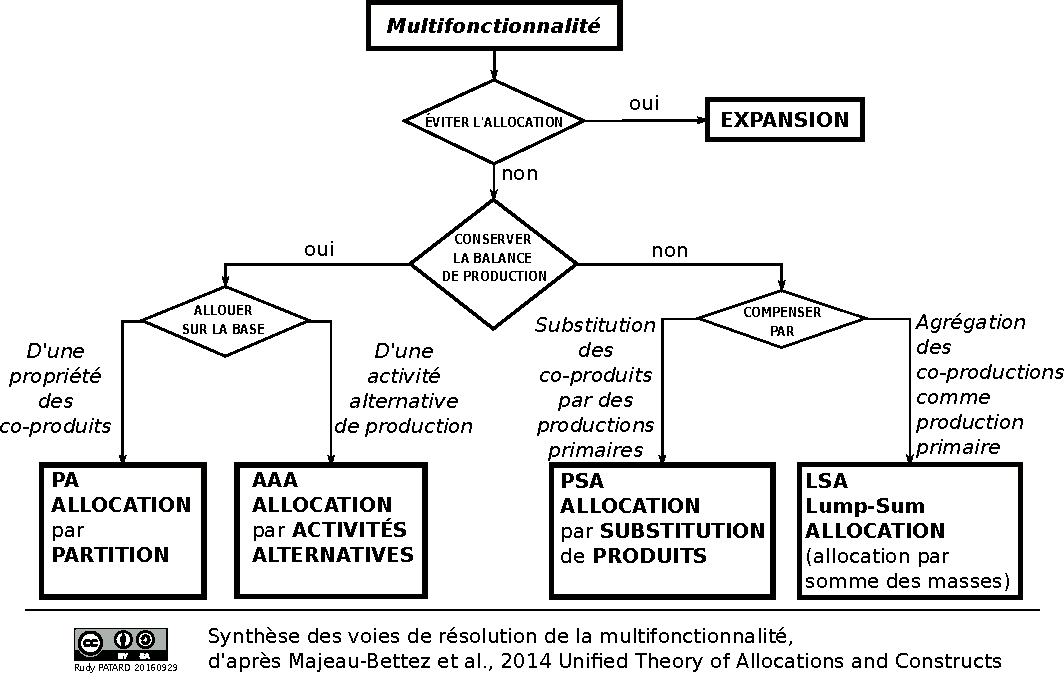
\includegraphics[width=\textwidth]{/home/rudy/Documents/rudy/01_These/11_production/01_COMMUNICATION/figures/allocation/Majeau-Bettez_classification.pdf}
\caption{Classification des approches de résolutions de la multifonctionnalité selon \citeauthor{majeau-bettez_unified_2014}.}
\label{fig:Majeau-classification}
\end{figure}


%Majeau-Bettez_classification.pdf

%Tout d'abord il faut saluer la performance de l'équipe de \citeauthor{majeau-bettez_unified_2014}, sans laquelle l'expression de mon modèle aurait d'une part été beaucoup difficile à exprimer et d'autre part aurait eu moins de prise.
Ce travail unificateur a ceci de remarquable que la poursuite d'une modélisation universelle ne semblait pas être un objectif commun dans la discipline.
En atteste la déclaration de \citeauthor{cherubini_influence_2011}~:
\blockcquote[traduction]{cherubini_influence_2011}{
Plutôt que de choisir une méthode d'allocation à adopter universellement dans toutes les évaluations, les analystes en cycle de vie devraient identifier \emph{la} méthode qui convient le \emph{mieux} à \emph{leurs} questions de recherche.
%Rather than selecting one allocation method to be universally adopted in all the assessments, LCA practitioners should identify the method which better fits their research questions}.
}\footnote{Voyez ici une position caractéristique du rationalisme constructiviste radicale \textit{dans une nuance de la théorie de la contingence}.
C'est à dire la considération d'une voie naturellement meilleure \textit{selon le contexte}.}

%Nous nuancerons toutefois l'apport de cette unification pour l'ACV par les points suivant sur l'étendu des méthodes unifiées par ce travail.


%+
\subsubsection{Hiérarchie standard}
Nous ferons référence à la hiérarchie de traitement de la multifonctionnalité de l'ISO en nous appuyant sur le document librement accessible du manuel ILCD~\cite{european_commission_ilcd_2010}.
Ce référentiel distingue trois niveaux, ou approches, de la multifonctionnalité.
Pour éviter toute confusion, nous les reprendrons dans leur libellé anglophone.

\textbf{\blockcquote[p.~74]{european_commission_ilcd_2010}{First approach: Subdivision of multifunctional processes}}

Le terme `procédé' est associé à `process' en anglais.
La distinction entre procédé et processus est donc plus visible en français.
Mais c'est dans les deux langues une notion d'échelle qui génère cette pseudo-multifonctionnalité.
Un procédé qui peut être divisé n'est pas un procédé unitaire.
C'est là toute l'importance de la distinction entre "unit process", procédé unitaire et "system process" système de procédé\emph{s} qui dans les fait n'est pas entièrement suivi dans les bases de données.
En atteste \citeauthor{majeau-bettez_unified_2014} \cite{majeau-bettez_unified_2014}
\blockcquote[traduction p.~3]{majeau-bettez_unified_2014}{
De même, il est encore pratique courante en ACV d’inventorier directement en termes de "procédés unitaires", normalisées, pré-alloués, qui fournissent collectivement une description du système symétrique.
Les activités co-productrices sont problématiques pour ces stratégies d'inventaires symétrique car il devient impossible de dissocier l'observation (inventaire) de la modélisation (allocation, etc.).
%Similarly, it is still common practice in LCA to inventory systems directly in terms of normalized, preallocated “unit processes,” which collectively provide a symmetric system description. Multioutput activities are problematic for such symmetric inventorying strategies because it becomes impossible to dissociate the observation (inventory) from the modeling (allocation, and so on).
}

\keybox{\textbf{La première approche de résolution de la multifonctionnalité} selon l'ISO et l'ILCD \textbf{ne la traite en fait pas}.
C'est la vérification d'être au niveau du procédé unitaire.}

\textbf{\blockcquote[p.~76]{european_commission_ilcd_2010}{Second approach: System expansion (including substitution)}}
Une des origines des problèmes de définition des différentes approches désignées par "expansion" se situe probablement ici.
Deux orientations de cette seconde approche sont traités sous des mêmes noms et sous l'un de ces nom (expansion) rien n'est proposé qui en soit réellement.

Sens \textbf{soustractif}.
Le premier sens de cette approche est celui de \textbf{la substitution} à une chose évitée.
Également décrite par crédit ou impacts évités, elle consiste à soustraire un système \emph{jugé} substituable au modèle étudié pour \emph{retirer} les co-fonctions de l'évaluation comparative.
L'argumentaire tient dans ce que la réponse multifonctionnelle déplacerait (réduirait) les productions primaires des co-productions respectives.
%"Terms and concepts: System expansion / substitution"
%"The first one is to solve the multifunctionality by expanding the system boundaries and substituting the not required function with an alternative way of providing it, i.e. the process that the not required function supersedes (“substitution”)."

Sens \textbf{additif}.
\textbf{L'expansion} est décrite dans l'ILCD comme l'addition au modèle étudié d'un ou plusieurs système, toujours afin de conserver l'équilibre des fonctions multiples.
\footnote{
\exbox{
\blockcquote[traduction p.~77]{european_commission_ilcd_2010}{
L'autre situation est lorsque plusieurs systèmes multifonctionnels (par exemple différentes marques d'un produit de consommation complexe) doivent être rendues comparables dans une étude comparative.
Cela se ferait en élargissant les limites du système et en ajoutant pour le cas donné les fonctions et inventaires des produits mono-fonctionnels respectifs manquants~: Par exemple, lorsque l'on compare un copieur combiné, imprimante, scanner, télécopieur avec un copieur combiné, scanner, fax, la fonction manquante de ``l'imprimante'' serait ajouté à l'inventaire du deuxième système de produit.
%The other situation is when several multifunctional systems (e.g. different brands of a complex consumer product) are to be made comparable in a comparison study. This would be done by expanding the system boundaries and adding for the given case missing functions and the inventories of the respective mono-functional products: E.g. when comparing a combined copier, printer, scanner, fax machine with a combined copier, scanner, fax machine, the missing function "printer" would be added to the inventory of the second product system"
}
}
}

\keybox{
Cette seconde approche expansion / substitution, ne relève que de la \emph{substituabilité}.
L'expansion pure n'est d'ailleurs pas présente au référentiel qui encadre l'ACV et son principe d'\emph{unicité de l'unité fonctionnelle}.
Une expansion à chaque co-fonctionnalité rencontrée en cas de multifonctionnalité empêche la considération d'égalité du service rendu des alternatives comparées.
}

\textbf{\blockcquote[p.~79]{european_commission_ilcd_2010}{Third approach: Allocation}}
\blockcquote[traduction, p.~79]{european_commission_ilcd_2010}{
Comme dernière approche dans la hiérarchie ISO, est nommée l'allocation, c'est le fait de partitionner des entrées et sorties entre les co-fonctions selon \emph{un} critère d'allocation.
%"As last step in the ISO hierarchy, allocation is named, partitioning the inputs and outputs
%between the co-functions according to some allocation criterion."
}

Dans cette troisième et 'dernière' approche désignée par \emph{allocation}, une seconde hiérarchie est présente.

Premièrement il s'agit de déterminer, si possible, la relation physique liant entrant et sortant.
%\footnote{
\blockcquote[p.~79]{european_commission_ilcd_2010}{
Si possible, selon la norme ISO 14044:2006, l'allocation doit être effectuée conformément à \emph{la cause physique  -- et, implicitement couvertes également~: les relation chimiques et biologiques -- sous-jacente} entre les différents produits ou fonctions.
Cela doit refléter la façon dont les entrées et les sorties individuelles sont quantitativement modifiés par des changements quantitatifs dans les multiples fonctions délivrées par le processus ou du système.
%If possible, according to ISO 14044:2006, allocation should be performed in accordance with the \emph{underlying causal physical - and implicitly also covered: chemical and biological - relationship} between the different products or functions. This should reflect the way in which the individual inputs and outputs are quantitatively changed by quantitative changes in the multiple functions delivered by the process or system.
}
%}.
\keybox{
La recherche de la cause physique est ici en fait une dernière tentative de subdivision et donc la détermination de sous-procédés, \textit{cf.} 1 ère approche.
Le praticien n'est potentiellement pas encore à l'échelle de la multifonctionnalité.
}

L’existence de relations entre paramètres d'entrées et de sorties soulève la distinction entre co-fonction à relation fixe ou variable.
Ceci est traitée par \citeauthor{weidema_avoiding_2000}~\cite{weidema_avoiding_2010,weidema_has_2014}, qui se reporte à la première approche si la relation est variable et à la seconde approche (substitution) si la relation est fixe, pour éviter la troisième dans les deux cas, fixe et variable.

%\colorbox{yellow}{creuser : Generalized Make and Use Framework for Allocation in Life Cycle Assessment} lien database - allocation pour savoir quand l'introduire.

Puis lorsque cela n'est pas possible, l'ILCD comme l'ISO propose de partitionner l'inventaire sur la base d'une relation économique ou sur la base d'une propriété des flux (des indicateurs de masse et d'énergie sont mentionnés).
%\footnote{
\blockcquote[traduction p.~79]{european_commission_ilcd_2010}{
Quand il est impossible de trouver des relations causales physiques communes claires entre les co-fonctions, l'ISO 14044:2006 recommande d'effectuer la répartition selon une autre relation entre eux.
Cela peut être une relation économique ou une relation entre une autre des propriétés (par exemple non-causales mais physique) des co-fonctions telles que le contenu énergétique qui est souvent utilisée dans la répartition entre les différents combustibles co-produits dans une raffinerie.
%When it is not possible to find clear common physical causal relationships between the co-functions, ISO 14044:2006 recommends performing the allocation according to another relationship between them. This may be an economic relationship or a relationship between some other (e.g. non-causal physical) properties of the co-functions such as energy content that is often used in the allocation between different fuels co-produced in a refinery.
}
%}.
\keybox{Les lecteurs attentifs auront compris que choisir \emph{une} unité pour la répartition est équivalent à dire `sur quel critère les flux sont substituable'.
Le repli à une allocation économique est donc une approche par substituabilité sur une base monétaire.
Le choix d'une clef énergétique est la considération d'une substituabilité énergétique.}

Mention particulièrement intéressante vis à vis de ces références (de 2006 et 2010), il est précisé que dans le cas d'impossibilité de subdivision, l'allocation est l'approche correspondante~\cite[p.~80]{european_commission_ilcd_2010}
%\footnote{
%\blockcquote[p.~79]{jrc_ilcd_2011}{
%Note that if subdivision cannot provide exclusively mono-functional unit processes that can be attributed to the analysed function, allocation is the corresponding method approach under attributional modelling for solving multifunctionality of processes.}
%}.
Cela ne tiens donc pas compte de la proposition de \citeauthor{weidema_avoiding_2000} faite en \citeyear{weidema_avoiding_2000} d'éviter systématiquement l'allocation par partition~\cite{weidema_avoiding_2000}.
Mais de toute façon dans sa présentation, jusqu'ici le résultat est soit l’inconsistance, soit une perspective de substituabilité.

\subsection{Détails des méthodes}
\label{subsec:Détails des méthodes}
%Par commodité nous ne redéveloppons pas le formalisme matricielle
%%\colorbox{yellow}{soit traitement par méthode, soit par thème}
%%Substituabilité, perspective temporelle, comparatif final
%
%reprendre la conclusion LSA ; AAA ; PSA ; PA ; Expansion / Partition
%
%\colorbox{yellow}{chercher l'ordre de présentation des méthodes pour limiter les redites}
%
%??? Traiter la question de la temporalité (attributional consequential) séparément pour les cas d'allocation spécifique conséq , subst ; attribut , partition
%
%\colorbox{yellow}{reprendre chaque sous-section avec un graphique type figure 2 de Majeau}

Avant même d'observer mathématiquement ces méthodes, il nous faut les distinguer.
Des nuances entre méthodes sont en effet à éclaircir et le titre d'une méthode est parfois employée pour désigner la voisine.
\blockcquote[traduction]{majeau-bettez_unified_2014}{
Pour distinguer ces deux techniques, car elles ont toutes deux été désignées simplement comme «l'expansion du système» dans la littérature (par exemple, Schmidt et Weidema 2007; Weidema et Schmidt 2010;. Cherubini et al 2011) -- nous avons pris la liberté de leur donner des noms spécifiques: allocation par activité alternative (AAA) et allocation de produit par substitution (PSA)
%To distinguish these two allocation techniques—because they have both been designated simply as “system expansion” in the literature (e.g., Schmidt and Weidema 2007; Weidema and Schmidt 2010; Cherubini et al. 2011)—we have taken the liberty to give them specific names:alternate activity allocation (AAA) and product substitution allocation (PSA)
}
"System Expansion" est en fait souvent "expansion substitution", soit PSA ou AAA (cf la suite de cette section).
Et évidement l'expansion pure est appelée expansion.
%\footnote{

%}.

Nous précisons également que sont considérés comme \emph{équivalents} sous les méthodes par substitution\footnote{Les lecteurs noterons ici l'emploi par \citeauthor{kim_allocation_2002} de "system expansion" pour le modèle PSA. La distinction dans leur article entre PSA et AAA tient au "displacement ratio", facteur de déplacement \ldots substituabilité quand tu nous tient.}~:
\begin{itemize}
\item les fonctions.
\exbox{
\blockcquote[traduction]{kim_allocation_2002}{
Pour compléter l'approche de l'expansion du système pour le procédé de broyage à sec, un système de produit dont la fonction est équivalente à la fonction d'huile de soja est aussi nécessaire.
%To complete the system expansion approach for the dry milling process, a product system whose function is equivalent to the function of soybean oil is required as well.
}
}
\item les impacts des filières
\exbox{
\blockcquote[traduction]{kim_allocation_2002}{
L'approche par l'expansion du système est équivalent à \emph{supposer que les charges environnementales} associés à l'éthanol à partir du broyage sec \emph{sont égaux} à ceux qui sont associés avec de l'éthanol à partir de mouture humide.
%The system expansion approach is equivalent to \emph{assuming that the environmental burdens} associated with ethanol from dry milling \emph{are equal} to those associated with ethanol from wet milling.
}
}
\end{itemize}

Parce que le formalisme mathématique développé par \citeauthor{majeau-bettez_unified_2014} est riche mais également difficile d'accès, nous proposons une représentation graphique de chacune des méthodes est proposées.
Les notations sont posées ainsi\footnote{Nous ne présentons ici que la fraction que nous utilisons du formalisme de \citeauthor{majeau-bettez_unified_2014}.}~:
\begin{description}
\item Les $z_{iJj}$ représentent les flux intermédiaires. $z_{iJj}$ est le flux de produit i dans l'activité J pour produire j.
\item Les lettres capitales et $\ast$ représentent les activités.
\item Les lettres minuscules et les $\bullet$ signifient les nécessités (commodités ou encore produits).
\item $v_{kJ}$ est un composant de la matrice de production (commodité k produite dans l'activité J).
\item $u_{iJ}$ est un composant de la matrice des utilisations, (commodité i employée dans l'activité J) consommations (`untraceable', sans traçabilité).
\item $g_{1,J}$ est la production (sortie) totale de l'activité.
\item ${a}_{iJk}$ sont les coefficients techniques (ici quantification de i dans l'activité J pour la production de k).
\item $a^{\Gamma}_{ik}$ sont les coefficients des alternatives technologiques (Alternate technology matrix) (coefficient alternatif de i pour la production de k)
\item $\mathcal{J}$ est le domaine des produits et activités \emph{secondaires}.
\item $\wp$ est le domaine des produits et activités \emph{primaires}.
\end{description}


Voyons donc maintenant que nous y sommes préparés ces méthodes.

\subsubsection{LSA~: Lump Sum Allocation}
Sous la méthode dite "Lump-Sum" la différence entre les coproductions est considéré comme négligeable~\cite[LSA]{majeau-bettez_unified_2014}
%\footnote{
%\blockcquote{majeau-bettez_unified_2014}{Differences between a primary product and its secondary product are assumed to be negligible.}
%}.
Pour la classification que nous donnerons ultérieurement, je propose de souligner l'hypothèse (différence négligeable) en la reformulant~: les coproduits sont \emph{substituables}.

\begin{equation}
 z_{iJj}=
 \begin{cases} a_{iJi}g_{J} = u_{iJ} \quad \forall(j,J)\wp,i\in \bullet 
 \\
 0 \quad \forall(k,J)\in \mathcal{J}|k = j,i\in \bullet
 \end{cases}
 \label{eq:Majeau unified equation LSA}
\end{equation}
L'équation~\ref{eq:Majeau unified equation LSA} a pour représentation graphique la figure~\ref{fig:Lump-Sum}
\begin{figure}[htbp]
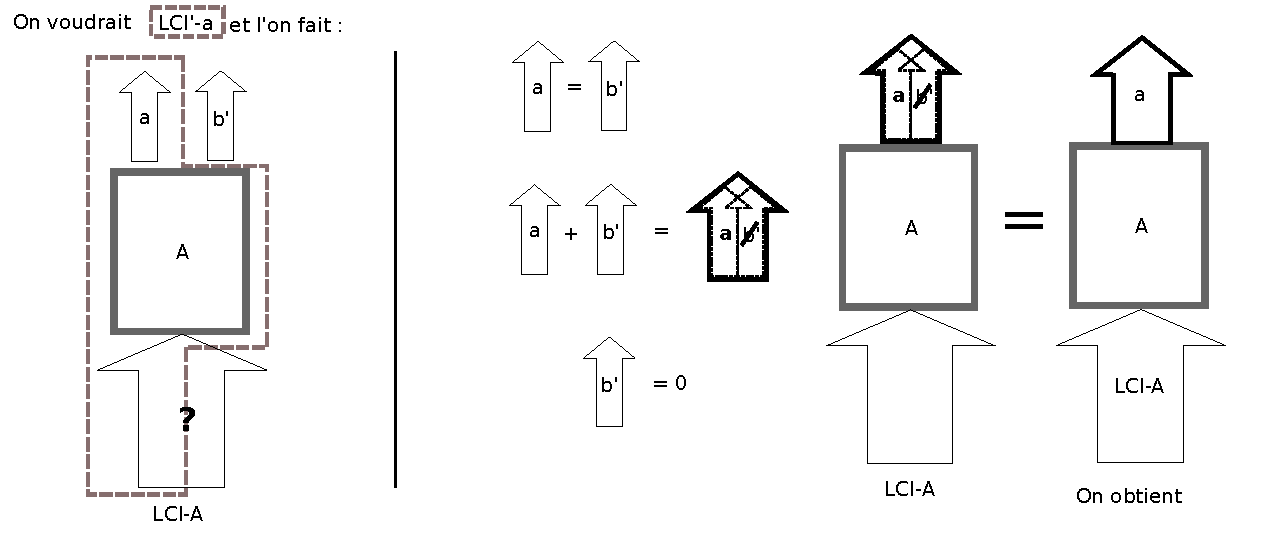
\includegraphics[width=\textwidth]{/home/rudy/Documents/rudy/01_These/11_production/01_COMMUNICATION/figures/allocation/LS_allocation.pdf}
\caption{Représentation de la méthode LSA.}
\label{fig:Lump-Sum}
\end{figure}

\figbox{Les flux relatifs aux commodités secondaire $\forall(k,J)\in \mathcal{J}|k = j,i\in \bullet$ sont considérés comme nuls.
Toute la production ($g_{J}$) est considérée comme primaire ($\wp$)
\exbox{\blockcquote[traduction. LSA]{majeau-bettez_unified_2014}{
Un champ de produisant de 5 tonnes (t) de céréales et 2 t de paille, [\ldots], serait modélisé comme la production, uniquement, de 7 tonnes de céréales.
%A field producing 5 tonnes (t) of grain and 2 t of straw, for example, would be modeled as producing 7 t of grain as its single output.
}
La somme est toujours de 7, mais les céréales passe de 5 à 7 et la paille de 2 à 0.
}
}



La somme groupée (LSA) ne respecte pas le principe de conservation des productions~\cite{majeau-bettez_unified_2014}.
Notez que nous considérons une conservation avec catégorisation.
La masse totale reste la somme de celles des coproduits.
Mais les flux, des coproduits non retenu, autant que du \textit{principal}, sont perturbés.
%Il nous parait peu légitime de développer plus encore des modes de décision ne respectant pas les lois connues de la physiques.
%Cela serait en tout cas poursuivre le développement des critiques à l'encontre de la méthode.
%Nous développerons plus particulièrement la question de la conservation des différentes "balances".

\subsubsection{PSA~: Product Substitution Allocation}

%\colorbox{yellow}{??? PSA et AAA dans une seule sous-section ???}

\begin{equation}
 \label{eq:Majeau unified equation PSA}
 z_{iJj}=
 \begin{cases} a_{iJj}v_{jJ} = u_{iJ} - \displaystyle\sum_{k|(k,J)\in\mathcal{J}} \xi_{ik}v_{kJ} \quad \forall(j,J)\wp,i\in \bullet 
 \\
 0 \quad \forall(j,J)\in \mathcal{J}|k = j,i\in \bullet
 \end{cases}
\end{equation}

La représentation de l'équation~\ref{eq:Majeau unified equation PSA} donne la figure~\ref{fig:PSA-FR}.
\begin{figure}[htbp]
\resizebox{1.00\textwidth}{!}{
\input{/home/rudy/Documents/rudy/01_These/11_production/01_COMMUNICATION/figures/allocation/PSA_allocation_xi.pdf_tex}
}
\caption{Représentation de la méthode PSA, avec un pont de procédé multi-fonctionnel (B-C).}
\label{fig:PSA-FR}
\end{figure}
\figbox{
Lisons conjointement l'équation~\eqref{eq:Majeau unified equation PSA} et la figure~\ref{fig:PSA-FR}.
Sur la représentation graphique, un 'pont' de substitution est représenté.
Pour accéder au produit b au sein du procédé multifonctionnel B, le coproduit c' et crédité à B depuis l'activité C, mono-productrice de c.
Les coproduits sont annulés dans l'activité traitée ($0 \forall(j,J)\in \mathcal{J}|k = j,i\in \bullet$) et la production \textit{principale} ($\forall(j,J)\wp,i\in \bullet$) est `crédité' au taux de déplacement près ($\xi_{ik}$) des fonctions, commodités ($v_{kJ}$) jugées substituées. % ($ a_{iJj}v_{jJ} = u_{iJ} - \sum_{k|(k,J)\in\mathcal{J}} \xi_{ik}v_{kJ} \forall(j,J)\wp,i\in \bullet $). 
}

Les produits secondaires pourrait tout à fait être exprimés sous le terme $\xi_{ik}v_{kJ}$.
Ainsi non "annulés", une version 'PSA balanced' (en fonction évidement, car ni en masse ni en aucune autre unité) pourrait donc exister (à hypothèse de substituabilité valide).
Il ne resterait qu'à définir les relations d'équivalence ($\xi_{ik}$), signifiant la différence des produits substitué l'un à l'autre.
Ceci donnerait~:
\begin{equation}
 z_{iJj}=
 \begin{cases} a_{iJj}v_{jJ} = u_{iJ} - \displaystyle\sum_{k|(k,J)\in\mathcal{J}} \xi_{ik}v_{kJ} \quad \forall(j,J)\wp,i\in \bullet 
 \\
 \xi_{ik}v_{kJ} \quad \forall(j,J)\in \mathcal{J}|k = j,i\in \bullet
 \end{cases}
 \label{eq:PSA-Majeau_Balanced}
\end{equation}
En somme c'est une formulation très proche du modèle AAA que nous verrons immédiatement après, au coefficient d'équivalence près.
\subsubsection{AAA~: Alternate Activity Allocation}

\begin{equation}
 z_{iJj}= a_{iJj}v_{jJ} =
 \begin{cases} u_{iJ} - \displaystyle\sum_{k|(k,J)\in\mathcal{J}} a^{\Gamma}_{ik}v_{kJ} \quad \forall(j,J)\wp,i\in \bullet 
 \\
 a^{\Gamma}_{ik}v_{kJ} \quad \forall(j,J)\in \mathcal{J}|k = j,i\in \bullet
 \end{cases}
 \label{eq:Majeau unified equation AAA}
\end{equation}


\begin{figure}[htbp]
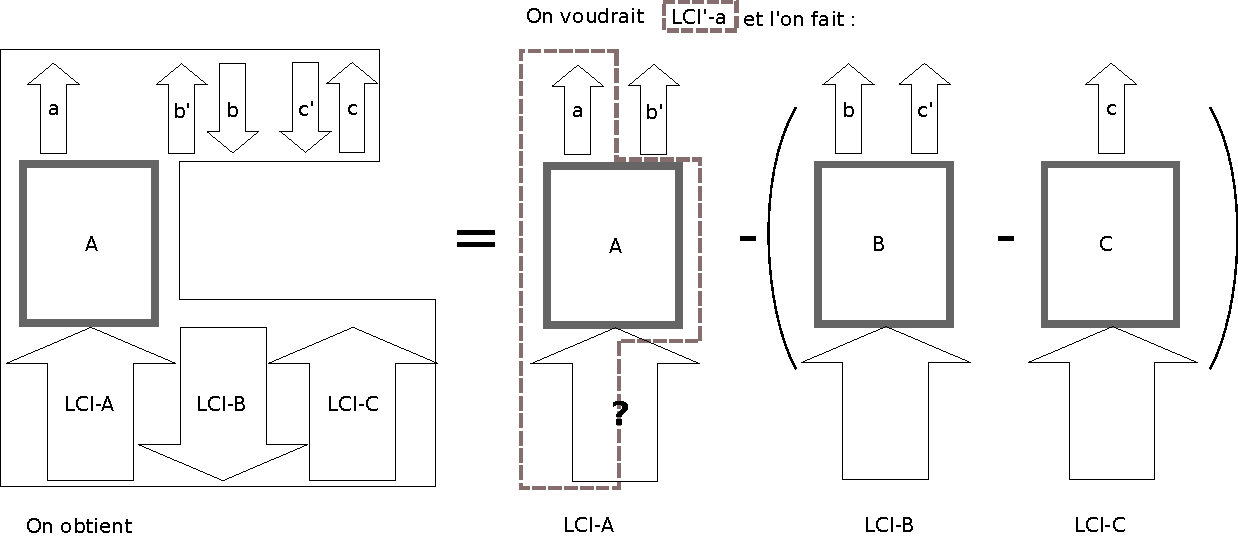
\includegraphics[width=\textwidth]{/home/rudy/Documents/rudy/01_These/11_production/01_COMMUNICATION/figures/allocation/AAA_allocation.pdf}
\caption{Représentation de la méthode AAA, avec un pont de procédé multi-fonctionnel (B-C).}
\label{fig:AAA-FR}
\end{figure}
\figbox{
L'équation \eqref{eq:Majeau unified equation AAA} est représentée dans la figure~\ref{fig:AAA-FR}.
La lecture est quasiment identique à Eq.\eqref{eq:Majeau unified equation PSA} et Fig.\ref{fig:PSA-FR} à ceci près que l'équivalence (du produit i au produit k) n'est pas donnée sur la base des produits avec $\xi_{ik}$ mais sur les procédés alternatifs par $a^{\Gamma}_{ik}$.

La nuance sensible dans entre l'expression (original) de PSA face à AAA est l'annulation des flux pour le domaine secondaire en PSA ($0 \forall(j,J)\in \mathcal{J}|k = j,i\in \bullet$).
}
%For example, one option is to ascribe to secondary coproducts the inputs that they would have required had they been produced as the primary product of some alternate activity (Figure 3:2.2) and ascribe the remainder of the joint requirements to the primary product.

%The total inputs and outputs of each activity remain identical to that recorded in the inventory (equation (8), decision variables ࢞U = ࢞V = 0). Thus, both primary and secondary productions remain available for intermediate or final use, that is, no observed flow is substituted, nothing is “avoided.”

AAA: "Alternate Activity Allocation" contient une contradiction dans sa présentation par \citeauthor{majeau-bettez_unified_2014}.
Les auteurs présentent cette méthode en indiquant qu'aucun flux observé n'est substitué et que rien n'est "évité" (référence à 'avoided burden').
%\footnote{
\blockcquote[traduction]{majeau-bettez_unified_2014}{
Le total des entrées et sorties de chaque activité reste identique à celui enregistré dans l'inventaire (équation (8) [de la publication d'origine], les variables de décision $ \Delta U = \Delta V = 0 $). Ainsi, les productions primaires et secondaires demeurent disponibles pour utilisation intermédiaire ou finale, i.e. \textbf{aucun flux observé n'est substitué, rien est "évité}."
%The total inputs and outputs of each activity remain identical to that recorded in the inventory (equation (8), decision variables $ \Delta U = \Delta V = 0$). Thus, both primary and secondary productions remain available for intermediate or final use, that is, no observed flow is substituted, nothing is “avoided.”
}
%}.
Or, ils décrivent également la méthode comme \blockcquote[traduction]{majeau-bettez_unified_2014}{
inscrivant aux produits secondaires, les flux qu'ils auraient requis s'ils avaient été produit en tant que production 'primaires' d'une activité alternative, laissant les autres flux nécessaires au produit primaire
}.
Les travaux cités en références sur cette méthode\footnote{
\blockcquote[traduction]{majeau-bettez_unified_2014}{
Des études telles que Cherubini et collègues (2011) et Weidema et Schmidt (2010) sont de bons exemples de cette modélisation
%Studies such as Cherubini and colleagues (2011) and Weidema and Schmidt (2010) are good examples of such modeling,
}},
traitent bien de commodités déplacées\footnote{
\blockcquote[traduction]{cherubini_influence_2011}{
le gaz naturel est supposé comme la source de chaleur et d'énergie déplacée
%natural gas is assumed as the source of the displaced heat and power
}.
\blockcquote[traduction]{weidema_avoiding_2010}{
Pour l'expansion du système, nous avons besoin du système supplémentaire de "bovins à viande», qui est \emph{déplacé} par la sortie supplémentaire de la viande de la vache laitière.}
Le système de la viande est exclusivement affecté la route des bovins de viande; c-a-d, dans le système étendu, aucune viande ne provient de vaches laitières.
%For system expansion, we need the additional system “meat cattle,” which is \emph{displaced} by the additional output of meat from the dairy cow.}
%The meat system is exclusively assigned the meat cattle route; that is, in the expanded system, no meat comes from the dairy cow.
}.
\textbf{Il s'agit donc bien de considérer une activité de \emph{substitution}.}
De même, une part des flux est évitée (soustraite) au produit 'principal' car présent au sein de l'alternative considérée.

%déjà critiqué par la communauté. \colorbox{red}{retrouver la ref}
L'AAA implique également d'après \citeauthor{majeau-bettez_unified_2014} certaines conditions nécessaires~:
%L'inventaire devrait être réparti entre différentes alternatives technologiques pour les co-productions \emph{secondaires}.
%Les conditions nécessaires au fonctionnement de ce système sont~:
\begin{itemize}
\item \blockcquote[traduction]{majeau-bettez_unified_2014}{la distinction robuste entre productions primaires et secondaires}
\item \blockcquote[traduction]{majeau-bettez_unified_2014}{la description d'une technologie alternative pour la production de chacun de ces co-produits "secondaires".}
\end{itemize}
Ce modèle fonctionne d'après les auteurs, même s'il n'y a pas de mono-production \textit{directement} pour chacun des co-produits immédiats grâce à un chaînage automatisé des ponts de substitution~\cite{majeau-bettez_unified_2014}.
Mais comment ce mécanisme d'allocation pourrait-il prendre fin sans procédé monofonctionnel pour chaque production à allouer "en bout de branche" (cf position du procédé C \ref{fig:AAA-FR})~?
Or, nous n'avons pas connaissance de procédé mono-flux.
Nous le développerons ultérieurement, la fonctionnalité est affaire de jugement et nous considérons des flux \emph{utiles} (jugement) comme fonctionnels.
Si nous complétons les éléments requis à la méthodologie AAA il faudra donc mentionner~: \emph{Jugement de substituabilité des produits entre-eux.}
%\colorbox{yellow}{brainstorming pour une annexe des flux non usuellement observés mais présent dans le but d'identifier un procédé mono-flux mono-fonctionnel ?}
%\begin{figure}[htbp]
%\includegraphics[width=\textwidth]{/home/rudy/Documents/rudy/01_These/11_production/01_COMMUNICATION/figures/allocation/Subsitution-fr.pdf}
%\caption{Représentation de la méthode PSA, avec pont de procédé multi-fonctionnel.}
%\label{fig:PSA-FR}
%\end{figure}
Le modèle nécessite l'existence systématique de procédés mono-fonctionnels, direct ou indirect, puisque chaque branche doit pouvoir s'arrêter.
L'absence de multifonctionnalité est théoriquement contournable car des cascades sont exploitables. 
\exbox{
Dans l'activité A produisant a,b et c~: A(ab'c'), a est `isolable' par B(bc'') ou B(b) + C(c) ou C(cb'') ou via P(pq'r'f') + T(tpb''') + V(vt') + Q(qs') \ldots
Les lecteurs comprendront aisément les limites pratiques à la possibilité théorique.
Car il est également crucialement requit que soient considérés substituables les différents produits modélisés (b' issu de l'activité A est considéré comme substituable à b de l'activité B etc.).
Ceci fait beaucoup de substitution à accorder.
D'où le commentaire de \citeauthor{heijungs_allocation_2007} d'un trop grand nombre d'hypothèses à gérer.
Et encore faut-il l'accepter même une seule fois.
}
Ainsi
$
%\begin{equation}
a \equiv ab' -(bc' -(cd' - d))\equiv a = ab -(bc -(cd - d))
%\end{equation}
$.
Et il en va de même pour les activités et leur impacts, comme précisé à l'introduction de cette section au \ref{subsec:Détails des méthodes}.

\subsubsection{PA~: Partitioning allocation, Allocation par partition}
L'allocation par partition est nécessaire pour l'évaluation comparative sur la base de l'\emph{unicité} de l'\gls{UF}, lorsque deux co-fonctions sont produites simultanément sans qu'il soit possible de les subdiviser en systèmes indépendants par les lois de la physique et dans une perspective de soutenabilité forte rejetant la substitution des produits ou des filières technologiques et leurs impacts.

Se pose la question~: Comment peuvent être allouées des parts de l'inventaire à chaque fonction résultante, chaque flux fonctionnel ?

Nous allons développer dans cette section ce mode de traitement de la multifonctionnalité.
Nous commençons ici par le présenter dans son état actuel.
%Allocation is needed when linked co-functions arise that cannot be subdivided into reduced systems by the laws of physics.

%How the allocate shares of the inventory to each resulting functions (functional flows)?
Certaines études cherchent la "meilleure" clef d'allocation (masse, énergie, devise), respectivement au champs d'application (carburant, nourriture, traitement des \emph{déchets} etc.)~\cite{silva_wood-based_2014, ayer_co-product_2006, cherubini_influence_2011}.
%Some studies search \emph{the best} allocation key (mass, energy, money) respectively to the application fields (fuels, food, waste treatment)~\cite{silva_wood-based_2014, ayer_co-product_2006, cherubini_influence_2011}.
%metal dubreuil ; 
%rejecting political ground Pelletier
%And this generate sector application specific rules.
\citeauthor{luo_allocation_2009} ont déclaré que \blockcquote{luo_allocation_2009}{mélanger les méthodes d'allocation dans un même cas d'étude n'est pas \emph{recommandable}}\footnote{
\citeauthor{luo_allocation_2009} dans cette étude traitent autant des méthodes que des clefs d'allocation au sein de la méthode par partition.
L'étude en question comprend d'ailleurs : la partition massique, économique et une expansion de système.
MA bio-CO2 exclu.
Economic Allocation
EA bio-CO2 exclu.
System Expansion.
La description de l'expansion sous-tend des coefficients de substitution de base physique.
L'\gls{UF} est composite mais unique.
\blockcquote{luo_allocation_2009}{
L'unité fonctionnelle utilisée dans les quatre solutions alternative est définie comme "un kilomètre de conduite automobile + valeur nutritive 13,6 kJ de maïs et de canne"\ldots
%The functional unit used in all four alternatives is defined as ‘one kilometre of car driving + nutritional value 13.6 kJ of corn and stover’\ldots
}
}, sans même justifier ce point de vu.
%\textsc{Luo} stated that \blockcquote{luo_allocation_2009}{mixing allocation methods in one case study is not advisable}.
Et de ce qui a été constaté, ce `mélange' n'est en effet pas réalisé (même application à tous le système).
Au mieux, différentes clefs sont testées en séquence en analyse de sensibilité ou pour un article à cette fin (comme ceux que nous discutons ici). % \colorbox{yellow}{!!!Reprendre les sources!!!}
%And from what we have observed, it is indeed not done.
%At best different allocation keys are sequentially observed.
Or, depuis le travail de \citeauthor{leontief_environmental_1970} il y a plus de \emph{quarante ans}, nous savons \emph{aujourd'hui} que l'ensemble de nos activités sont interconnectées~\cite{leontief_environmental_1970}. Donc, employer \textbf{une} \emph{règle sectorielle} pour calculer les allocations sur \emph{un système technico-social, \textbf{interconnectant} de fait \textbf{des secteurs différents}}, \emph{n'est pas adéquat}.
%But since the work of \textsc{Leontief}, we know all activities are connected~\cite{leontief_environmental_1970}.
%So using the rule of a particular sector and calling on a complete system seems inadequate.

Ce traitement monodimensionnel de l'allocation a été synthétisé par l'équipe \citeauthor*{majeau-bettez_unified_2014}.
Le principe énoncé est le suivant~:
~\blockcquote{majeau-bettez_unified_2014}{Toute allocation respectant la balance de production, qui répartisse les inventaires des nécessités sur les coproduits est représentée de manière générale par l'équation}
Eq.\eqref{eq:Majeau_unified_equation}

%\vspace{-.1cm}
\begin{equation}
 z_{iJj}=a_{iJj}v_{jJ} =
 \begin{cases} u_{iJ} - \displaystyle\sum_{k|(k,J)\in\mathcal{J}} \underline{a}_{iJk}v_{kJ} \quad \forall(j,J)\wp,i\in \bullet 
 \\
 \underline{a}_{iJk}v_{kJ} \quad \forall(k,J)\in \mathcal{J}|k = j,i\in \bullet
 \end{cases}
 \label{eq:Majeau_unified_equation}
\end{equation}
Avec les coefficients techniques exprimés par Eq.~\eqref{eq:technical_requirement_coefficient_majeau}
%with the technical coefficient expressed by: % \eref{eq:technical_requirement_coefficient_majeau}:
\begin{equation}
\underline{a}_{iJk}=u_{iJ}\frac{\psi_{kJ}}{\displaystyle\sum_{j\in\bullet}\psi_{jJ}v_{jJ}} \forall k|(k,J) \in \mathcal{J},i \in \bullet,J \in \ast
\label{eq:technical_requirement_coefficient_majeau}
\end{equation}
\figbox{
Aux flux utilisés (U) \emph{i} dans l'activité \emph{J} pour produire (V), de façon principale ($\wp$) la commodité \emph{j}, sont retirés des parts affectés aux coproductions secondaires ($\forall(k,J)\in \mathcal{J}|k = j,i\in \bullet$) sur la base de leur part suivant la clef d'allocation $\psi_{jJ}$, i.e. la part (fraction) $\frac{\psi_{kJ}}{\displaystyle\sum_{j\in\bullet}\psi_{jJ}v_{jJ}}$.

Pour rappel, 
\begin{description}
\item Les composants $z_{iJj}$ représentent les flux intermédiaires,
\item Les lettres capitales et $\ast$ représentent les activités.
\item Les lettres minuscules et les $\bullet$ signifient les nécessités (commodités).
\item $v_{kJ}$ composent la matrice de production.
\item $u_{iJ}$ composent la matrice des utilisations, consommations (untraceable, sans traçabilité).
\item ${a}_{iJk}$ sont les coefficients techniques.
\item $\mathcal{J}$ est le domaine des produits et activités \emph{secondaires}.
\item $\wp$ est le domaine des produits et activités \emph{primaires}.
\end{description}
}
%with $z_{iJj}$ the modelled intermediate flows, upper-case letters representing activities ; lower-case letters and $\bullet$ stand for commodities.
%$v_{kJ}$ is the supply matrix (productions).
%$u_{iJ}$ is the use matrix (untraceable).
%${a}_{iJk}$ are the technical coefficients (technical requirements).
%$\mathcal{J}$  is the domain of secondary products and activities.
%$\wp$ is the domain of primary products and activities.
\exbox{Prenons un exemple simple~:\\
%\newline
Dans l'activité \textbf{A}, à partir de~:
\begin{itemize}[noitemsep]
\item la consommation de 3~l de \textbf{s},
\item la consommation 1~kWh d'électricité \textbf{f}
\item l'émission de 10~g de \textbf{x} dans l'air
\item etc,
\end{itemize}
sont conjointement produits~:
\begin{itemize}
\item 100 unités de \textbf{a} pour une masse de 2~kg  (0.020~kg/unité) et un prix de 10~k€
\item 20 unités de \textbf{b'} pour un total de 1~kg (0.05~kg/unité) pour 2~k€.
\end{itemize} 

L'inventaire de l'activité A (les 3~l de \textbf{s}, le kWh d'électricité \textbf{f}, l'émission de 10~g de \textbf{x} dans l'air etc) est réparti~:
\begin{itemize}[noitemsep]
\item à 2/3 pour \textbf{a} et 1/3 pour \textbf{b'} suivant une clef massique.
\item à 5/6 pour \textbf{a} et 1/6 pour \textbf{b'} suivant une clef monétaire.
\end{itemize} 
Voyons comment, \emph{en suivant le formalisme présenté}\footnote{Ce qui brisera l'aspect de complexité de la formulation.}.\\
Soit \textbf{a}, arbitrairement le produit principal.
Prenons le cas de la clef massique.
Les 2/3 sont constitués sur la base du total (1), moins la part du secondaire (1/3), tel que présenté dans le développement suivant.\\
Le flux d'électricité \textbf{f}, alloué à la production de \textbf{a} dans l'activité A, c'est à dire $z_{fAa}$ est tel que\footnote{Le développement est présenté avec l'information dimensionnelle. N signifie Nombre d'Unité Produite.
Bien que sans dimension nous pensons que ces 'quantité d'item' aiderons la lecture.}~:\\
$z_{fAa} = u_{fA} - u_{fA} \times ( \frac{\mathit{masse_{b'A}/N_{b'A}}}{\mathit{masse_{b'A}/N_{b'A}}\times\mathit{N}_{b'A} + \mathit{masse_{aA}/N_{aA}}\times\mathit{N}_{aA}}) \times \mathit{N}_{b'A}\\
z_{fAa} = 1(kWh) - 1(kWh)(\frac{0.05(kg/N)}{0.05(kg/N)\times20(N_{b'A}) + 0.02(kg/N)\times100 (N_{aA})}) \times 20 (N_{b'A})\\
z_{fAa} = 1-1(\frac{1}{3})= 2/3 (kWh)$
}
Où se trouve le jugement de préférence dans cette équation générale \eqref{eq:Majeau_unified_equation}~?
Sous le PA, en dehors de la présence d'\emph{une} clef d'allocation, qui de fait est celle implicitement jugée comme \emph{absolument} plus importante que tout autre, il n'y en a pas de trace\footnote{Concernant PSA, AAA, LSA}.
%Where lies the preference judgement within the original equation that was stated in LCA theoretical framework?
%%Are preferences stated here?
%Apart from the fact that the allocation key used is the implicit \emph{single} important parameter, preferences are not stated here. %there is nothing more.
%\vspace{-0.3cm}
\subsubsection{Éviter l'allocation : expansion}
Nous commençons par présenter des avis divergents sur cette \textit{expansion}.
Puis nous exposons la pratique et la pensée derrière le terme.
Enfin nous présentons que l’expansion pourrait être.

\citeauthor{weidema_avoiding_2000} a avancé~\cite{weidema_avoiding_2000}, puis maintenu~\cite{weidema_avoiding_2010} que cela était \emph{toujours} réalisable.
%Mais c'est autre chose que l'expansion qui est défendu.
% \footnote{
\blockcquote[traduction]{weidema_avoiding_2000}{
Dans cet article, je conclus que l'allocation peut (et doit) \textbf{toujours} être évitée en ACV prospective. En ACV rétrospective, il est impossible d'exprimer un impératif concernant quelle procédure d'allocation appliquer, mais éviter l'allocation peut \textbf{toujours} être une option.
%In this article, I conclude that allocation can (and shall) always be avoided in prospective LCAs. In retrospective LCAs, it is not possible to express an imperative regarding what allocation procedure to apply, but avoiding allocation may still be an option.
}
%D'autres considèrent que l'expansion repose sur trop d'hypothèses et devrait être laissée hors d'un outil scientifique.
%\footnote{

Or, ceci n'est par exemple pas possible lors d'un examen comparatif entre deux co-production de même fonction (l'isolation de b' et b'' en traitement par substitution de b' et b''), car cela rejetterait l'hypothèse fondamentale de la méthode ($b' \equiv b''$)~\cite{kim_allocation_2002}.
%retrouver la ref sur system expansion SUBSTITUTION 
%\footnote{
%\exbox{
\blockcquote[traduction]{kim_allocation_2002}{
Cependant, cette approche [expansion - substitution] ne fonctionnerait pas pour une étude d'ACV dans lequel le but est de comparer les charges environnementales entre les différentes technologies de production d'éthanol.
%Une approche par l'expansion possible du système, qui pourrait atteindre l'objectif d'une telle étude ACV, serait de répartir les charges environnementales soit la farine de soja ou de l'huile de soja dans le système de broyage du soja en fonction des propriétés physiques ou des valeurs économiques, même si les procédures d'allocation ne seraient pas éliminées.
%However, \textbf{this approach would not work for an LCA study in which the goal of a study is to compare the environmental burdens between different ethanol production technologies}. A possible system expansion approach, that could meet the goal of such an LCA study, would be to allocate the environmental burdens to either soybean meal or soybean oil in the soybean milling system based on physical properties or economic values even though the allocation procedures would not be phased out."
}
%\citeauthor{kim_allocation_2002} expliquaient en effet que~:\blockcquote[traduction]{kim_allocation_2002}{
%L'hypothèse sous-jacente à l'approche de l'expansion du système est que les systèmes de produits avec une fonction équivalente ont les mêmes charges environnementales [9]. Par conséquent, les charges environnementales associées à l'éthanol à partir du broyage à sec sont supposés être équivalentes à celles qui sont associés à de l'éthanol à partir de broyage humide.
%%The underlying assumption in the system expansion approach is that product systems with an equivalent function have the same environmental burdens [9]. Hence, the environmental burdens associated with ethanol from dry milling are assumed to be equivalent to those associated with ethanol from wet milling.
%}
La littérature ne propose alors pas d'autre alternative que la proposition actuelle de partition.

\blockcquote[traduction]{cherubini_influence_2011}{
[\ldots] Tandis que Heijungs et Guinée analysent la logique et les problèmes, à la fois l'expansion et du partitionnement, ils concluent que la méthode d'expansion du système est généralement basée sur un trop grand nombre d'hypothèses, qui "doivent de préférence être laissées à l'extérieur d'un outil principalement scientifique" (Heijungs et en Guinée, 2007)~\cite{heijungs_allocation_2007}\footnote{\blockcquote[traduction]{heijungs_allocation_2007}{
Il apparaît que pour approcher les charges évitées, le nombre de "et si~?" hypothèses est si grand que les ACV sur le même sujet conduisent à des résultats assez divergents.
Puisque les questionnement "et si~?" ne peuvent pas recevoir de réponse non ambiguë, ces questions devraient de préférence être laissés à l'extérieur d'un outil principalement scientifique.
%It appears that for the avoided burdens approach, the number of ‘what-if’ assumptions is so large that LCAs on the same topic lead to quite diverging results.
%Since ‘what-if’ questions cannot be answered in an unambiguous way, such questions should preferably be left outside of a primarily scientific tool.
}.
%while Heijungs and Guinée analyze the logic and problems of both partitioning and system expansion, concluding that the system expansion method is usually based on a too large number of assumptions, which “should preferably be left outside of a primarily scientific tool” (Heijungs and Guinée, 2007).
}}.

{
%L'argumentation du début des années 2000 était la suivante.
%\blockcquote{weidema_avoiding_2000}{
%Because a system expansion may involve processes that also have multiple products, it has been suggested that there are situations in which system expansion
%would be impossible because it would involve an unending regression.
%}
%What is the counter argument on this point.
%> use "the market-based method of Weidema and colleagues (1999)"
%>> then it is an economic study
%
%information is lost in economical agregation
%
%there is no remaining information to build another judgment.
%
%> expansion = economic allocation + product and impact substituability
%{
%%FAIRE UNE TABLE AVEC ARGUMENTAIRE // CONTRE ARGUMENTAIRE WEIDEMA pour aider à la reformulation
%%
%%Trouver une autre forme de tableau (2 cases dessus, une case dessous)
%%thèse anti-thèse synthèse
%%|arg|contre-arg|
%%
%%|commentaire|
%
%%\begin{landscape}
%%\begin{longtabu} to \textwidth{some columns}
%%\caption[my caption]{my caption}
%%table code here
%%\end{longtabu}
%%\end{landscape}
%
%%\begin{landscape}
%%%\begin{longtabu} to \textwidth{some columns}
%%%\caption[my caption]{my caption}
%%%table code here
%%%\end{longtabu}
%%
%%\begin{longtable}{| p{7cm} | p{7cm} | p{5cm}|}
%%The following four obstacles to system expansion can be seen as part of the reason why thisoption has not generally been applied as a way toavoid allocation: & 
%%In this article, I conclude that allocation can(and shall) always be avoided in prospectiveLCAs. In retrospective LCAs, it is not possibleto express an imperative regarding what allocation procedure to apply, but avoiding allocationmay still be an option. I reach this conclusion byshowing how to overcome the four obstacleslisted above: & 
%%Commentaire\\ 
%%\hline
%%The following four obstacles to system expansion can be seen as part of the reason why this option has not generally been applied as a way to avoid allocation:  &
%%... I reach this conclusion by showing how to overcome the four obstacles listed above:  &
%%Commentaire\\ 
%%\hline 
%%1. In retrospective LCAs, there is typically no possibility for system expansion.
%%Retrospective studies typically seek to describe a status quo situation, in which there are no changes in production volume.
%%This obviously excludes the possibility of system expansion, because an expansion involves balancing a change in output volume of a co-product in one system with an equivalent change in the other systems to be compared, in order to maintain comparable product outputs from the systems.
%%The distinction between retrospective and prospective studies and its important consequences for the methodology (including the handling of co-products) has only recently been clarified (Tillman 1998; Weidema 1998).
%%It is still common to see retrospective studies applied for prospective purposes and a mix of methodologies and justifications without clear reference to the retrospective or prospective nature of the study.  &
%%1. By distinguishing clearly between retrospective and prospective studies (see next section)
%%, it is possible to distinguish between the situations in which system expansion is both possible and mandatory (prospective studies) and the situations in which system expansion is irrelevant or at least optional (retrospective studies).  &
%%Les études qualifiées de "retrospective" au sens attributionnelle ont tout autant que les études conséquentielles "prospective" un horizon temporelle incluant le futur et le passé.
%%Elles portent donc toutes des considérations sur les évolutions des productions et des marchés (output volumes).
%%L'hypothèse de volumes constants (que l'on retrouve en hypothèse pour l'inversion de Leontief) serait problématique pour tant pour l'antériorité (horizon temporel passé) que pour le futur.
%%Le premier argument 'contre' une expansion qui modifierait les volumes de production et donc valide, non pas pour les prospective ou retrospective mais pour toute partie historique des deux types d'études.
%%\\ 
%%2. It has been regarded as too difficult, too uncertain, or even impossible to identify which processes are affected when balancing a change in demand for (or supply of) a specific co-product.  &
%%2. By applying the market-based method of Weidema and colleagues (1999), I show that it is always possible, and seldom difficult, to identify the processes affected by a change in demand.
%%The uncertainty of this determination and the fundamental uncertainty of future market situations are inherent to the method, but can be neither a theoretical nor a practical argument against system expansion. &
%%La substitution par critère économique des produits maintien l'expansion substitution dans l'hypothèse de soutenabilité faible (qu'il s'agisse de la variante AAA ou PSA).
%%Plus qu'une question de difficulté, c'est une question de jugement sur la substituabilité pour la soutenabilité qui s'oppose à ce principe.\\ 
%%3. Because a system expansion may involve processes that also have multiple products, it has been suggested that there are situations in which system expansion would be impossible because it would involve an unending regression.  &
%%3. The problem of unending regression is eliminated by applying the method mentioned above, which provides clear cut-off criteria (a process is either included or excluded from the studied system) and reduces the number of processes that may possibly be involved in a system expansion (for details, see the section called: “Displaced Processes that Have Multiple Products”).
%%(ladite section)> When a displaced process yields not only the displaced product, but also other co-products, these co-products are also displaced and the demand for them must now be met in another way.
%%Thus, the procedure must be repeated for these co-products, but with a negative sign.
%%If this leads again to another process with multiple products, one might fear that this system expansion would continue without end.
%%The number of possible processes involved in the system expansion, however, is limited by the very procedure, because:
%%• the number of markets affected by each displaced process is limited, and the displaced process is only that specific supplier to each market, which is most sensitive to a change in demand,
%%• the four rules for system expansion provide clear cut-offs between the different product systems involved (a process is either included or excluded from the studied system),
%%• for each time the system expansion is iterated, both the economic value and the volume of the displaced processes tend to decrease, because in each iteration the avoided product is the determining coproduct of the displaced process and therefore typically of higher value (and often also larger in quantity) than the dependent coproducts, which go on to the next iteration. &
%%Double emploi du contre-argument 2 : Substituabilité sur la base de critère économique.
%%Question de suite géométrique de raison inférieure à un pour la convergence.\footnote{Raison inférieur à un sur l'hypothèse que le produit de susbstitution (co-produit) est de moindre qualité que le produit de même fonction déplacé. Cette commodité déplacée, "primaire", est (hypothèse) également produit en plus grande quantité.}
%%La fraction déplacé tend vers zéro.
%%C'est la base du raisonnement économique.
%%Il est donc mathématiquement juste.
%%Mais les mathématiques sont pour les modèles et comporte des hypothèses.
%%Il y a, non pas substituabilité entre un petit nombre de produits mais bien sur l'ensemble des "marchés".
%%Une commodité hors de la sphère monétaire mets par exemple quelques grains de sable dans ce "modèle".
%% \\ 
%%4. When a by-product does not substitute for another product, system expansion may be regarded as incompatible with the requirement that compared systems must have identical functions.  &
%%4. It is shown that by-products practically always substitute for other products, and even when this may not be the case, the studied systems are still comparable. &
%%"by-products practically always substitute for other products" On what basis, {{citation needed}}, authority etc.
%%"the studied systems are still comparable."
%%> Confrontation de paniers de fonctions différentes à évaluer tout de même (plus tard).
%%La multifonctionnalité n'a pas été résolue elle est repoussé.
%% \\ 
%%\hline
%%\caption{Argumentaire de Bo Weidema sur l'expansion en 2000}
%%\label{tab:expansion_weidema_arguments}
%%\end{longtable}
%%\end{landscape}
%}
}
Or, grattons un peu la surface et voyons les mécanismes et arguments employés par ses défenseurs.

\citeauthor{weidema_avoiding_2010} posent l'expansion comme conservatrice des balances et la partition (allocation) comme systématique perturbatrice.
%\footnote{
\blockcquote[traduction]{weidema_avoiding_2010}{
Ici, il est intéressant de noter que \textbf{l'expansion du système assure toujours des bilans de masse et de l'énergie, alors que l'allocation échoue presque toujours ce test}.
En bref, l'allocation brise le système original en deux systèmes artificiels ou plus selon une clé de répartition, et le seul équilibre qui reste intact dans les systèmes résultant est celui donné par la clé de répartition.
%Here, it is interesting to note that \textbf{system expansion always ensures mass and energy balances, whereas allocation nearly always fails this test}.
%In brief, allocation breaks up the original system into two or more artificial systems according to an allocation key, and the only balance that remains intact in the resulting systems is that given by the allocation key.
%With mass allocation, the mass balance remains intact, but energy and elemental balances are skewed; with economic allocation, none of the physical balances remains intact except if by chance a physical parameter follows the price of the products.
[\dots]
Avec l'expansion du système, les processus unitaires affectés sont agrandis ou réduits, mais il n'y a pas de partition artificielle, et parce que les systèmes qui en résultent sont de simples sommes des procédés unitaires concernés, dont chacune \textbf{maintient ses équilibres physiques intacts}, les systèmes résultant ont aussi tous leurs équilibres physiques intacts.
%With system expansion, the affected unit processes are scaled up or down, but there is no artificial partitioning, and because the resulting systems are simple sums of the affected unit processes, each of which \textbf{maintains its physical balances intact}, the resulting systems also have all physical balances intact.
}
%}.

Nuançons dès maintenant l'affirmation de \citeauthor{weidema_avoiding_2010} sur la conservation en extension.
"unit processes are scaled up or down", lorsque les procédés employés sont "mis à l'échelle", les volumes de leurs productions et consommations sont modifiés.
Donc les procédés appellent ou émettent des quantités, soit plus faibles, soit plus grande dans le système de production générale.
Celui-ci s'en trouve donc perturbé.
%\colorbox{yellow}{SCHEMA + FORMULE pour appuyer ce très juste propos}

Les propos de \citeauthor{weidema_avoiding_2010} pourraient paraître d'autant plus curieux face à la classification de \citeauthor{majeau-bettez_unified_2014} (Two General Allocation Strategies) où seuls PA et AAA conservent les bilans de produits~\cite{majeau-bettez_unified_2014}.
%D'autant plus que selon cet article, l'approche par \emph{partition} conserve les balances.

Lors de ces affirmations il est question \emph{des} balance\emph{s} globale et locales, balance du système et balances des procédés.
C'est a dire que pour \citeauthor{majeau-bettez_unified_2014} 
%\colorbox{yellow}{(autres publi sur la conservation)}
l'ensemble des produits initialement non alloués est conservé sur l'ensemble des allocations.
\textbf{La somme des parties reste égale au tout.}
\citeauthor{weidema_avoiding_2010} indiquent eux que pris en isolation, le "modèle de système unitaire monofonctionnel", \emph{lui} n'est plus équilibré.
Nos théoriciens semblent s'opposer, mais ils ne traitent pas des même équilibres.
%Ce modèle n'a bien sûr pas d'existence autre que théorique.

Voyons d'autres arguments.
\blockcquote[traduction]{weidema_avoiding_2010}{
En appliquant la méthode de Weidema et collègues (1999) \textbf{basée sur le marché}, je montre qu'il est toujours possible, et rarement difficile, d'identifier les processus affectés par un changement dans la demande [identifier le substitut]. L'incertitude de cette détermination et de l'incertitude fondamentale des futures situations de marché sont inhérentes à la méthode, mais ne peut être un argument ni théorique ni pratique contre l'expansion du système.}
%By applying the market-based method of Weidema and colleagues (1999), I show that it is always possible, and seldom difficult, to identify the processes affected by a change in demand. The uncertainty of this determination and the fundamental uncertainty of future market situations are inherent to the method, but can be neither a theoretical nor a practical argument against system expansion.}
\blockcquote[traduction]{weidema_avoiding_2010}{
%Tout d'abord,
[\ldots] l'allocation implique généralement une partition plus ou moins arbitraire du processus de co-production sur ses co-produits, sans tenir compte de la mesure dans laquelle un changement dans la quantité de ces co-produits affecte réellement la sortie fonctionnelle et d'autres échanges de la co-production processus.
%Deuxièmement, l'allocation ne tient pas compte des effets qu'un co-produit peut avoir sur le sort ultérieur des autres coproduits, qui est, les effets de déplacement et un traitement supplémentaire des co-produits avant le déplacement a lieu.
%First, allocation typically involves a more or less arbitrary partitioning of the co-producing process over its co-products, without consideration of the extent to which a change in the amount of these co-products actually affects the functional output and other exchanges of the co-producing process. Second, allocation ignores the effects that a co-product may have on the further fate of the other coproducts, that is, displacement effects and additional treatment of the co-products before displacement takes place.
}
Cela apparaît clairement, ce qui est désigné par l'expansion est en fait de la substitution sur la base majoritaire d'une allocation économique (via le marché).

Vous l'aurez compris, l'antagonisme a pour centre la subjectivité.
Des thèses différentes s'opposent sans que ne soit attaqué leur fondement commun.\\
A: Tout est toujours substituable sous critère économique.\\
Donc il est mathématiquement toujours possible d'appliquer l'expansion-substitution.\\
B: La substituabilité elle-même est une hypothèse problématique. Partitionner requière l'emploi de critères subjectifs.\\
A':Ce modèle (partition) repose sur le choix \href{http://www.cnrtl.fr/definition/arbitraire}{arbitraire} de la clef d'allocation.\\
B':Les hypothèses de substituabilité ne sont pas gérables\ldots\\
Ce qui n'est pas remis en cause est qui sous-tend les deux parties est qu'il y ait à trouver une unique et réelle description monofonctionnelle du système.


Ce qui est décrit comme problématique par \citeauthor{weidema_avoiding_2010} est en fait une incompréhension entre un objectif d'allocation pour produire une \emph{observation} ou celle avançant déjà dans l'\emph{évaluation}.
Il ne s'agit de modéliser des procédés unitaires monofonctionnels.
Ceux-ci n'existent pas.
C'est ce que frôlent du doigt \citeauthor{cruze_allocation_2014}.
Selon eux toutes les formes d'allocation sont juste.
Elles ne font qu'éclairer le problème de manière incomplète sous l'angle sélectionner pour l'attribution d'une part de l'inventaire.
\blockcquote[traduction]{cruze_allocation_2014}{
L'allocation par partition n'explore seulement qu'un petit sous-ensemble de solutions à un problème qui est mal posé en ce sens qu'il n'a pas une seule solution, mais potentiellement une infinité de solutions.
%partitioning explores only a small subset of solutions to a problem that is ill-posed in the sense that (1) it does not have just one solution, but potentially infinitely many solutions
}
Mais ces auteurs rejettent la piste de la subjectivité pour retomber dans le dogme de la donnée et du technocratisme.
\blockcquote[traduction de la conclusion]{cruze_allocation_2014}{
Plutôt que de compter sur une partition, une meilleure approche serait de rechercher des données supplémentaires ou un jugement d'expert afin que au moins le paramètre d'intérêt (l'inventaire monofonctionnel) devienne estimable.
%Rather than relying on partitioning, a better approach
%would be to seek out additional data or expert judgment so that
%at least the parameter (single product inventory) of interest
%becomes estimable.
}

Nous n'avons pas à les modéliser.
Construire l'inventaire, c'est déjà évaluer.
Mais pour accepter cela, il faut intégrer la subjectivité intrinsèque de la démarche d'évaluation.
Nous noterons à nouveau qu'une approche par expansion (ici sans substitution ni mise à l'échelle) permettrait de retarder l'usage du jugement mais pas de sans passer.


\keybox{
\textbf{"Avoiding allocation"}, les procédés sont multifonctionnels, prenons les comme tels.
Mais cette position revient à devoir observer et évaluer des alternatives sur des bases fonctionnelles différentes.
Pour conserver ces fonctions, le principe devrait reposer sur l'extension du système étudié.
Ceci implique de confronter non plus les alternatives sur la seule base de l'unité fonctionnelle, mais sur l'ensemble des fonctionnalités résultantes.
Traiter le jugement de valeur en fin de méthode n'est en rien une méthode de traitement.
C'est un ordonnancement de tâches, pas leurs réalisations.
}
Et parce que les praticiens comme les théoriciens ont jusqu'ici jugé nécessaire de conserver l'\emph{unicité} de l'unité fonctionnelle, c'est une approche par substituabilité qui suit généralement (cf les deux sous-section précédentes).


Hors amalgame de désignation Expansion - Substitution, observons un dernier point.
Pour traiter d'un procédé A donnant a et b', l'analyse est étendue.
Mais dans l'amont et l'aval des activités liées à a comme b' se trouvent d, e, f etc.
S'en suivra donc l'évaluation d'un quantum de a à une autre fraction de a' mais plus exactement a(+ d, e, f, etc.) face à a'(+ m,n,o,p etc.).
\keybox{
Ces ensembles de fonctions (comme l'ont justement souligné \citeauthor{weidema_avoiding_2010}) naîtront à des temporalité différentes, tout comme leurs impacts.
Pour tenir compte des horizons temporels choisis,
%(cf section \ref{label})
comme des phénomènes de concentration pour les impacts
%(cf section \ref{label})
,
il faudra probablement en terme d'ordonnancement commencer par l'expansion avant de réaliser le traitement de la multifonctionnalité.
La question sera donc finalement de traiter une évaluation comparative sur la base d'une unité fonctionnelle unique ou de réaliser un choix parmi des alternatives conduisant à la confrontation de groupes de fonctions de quantités et de natures variables.
}

%\subsubsection{Partitionner}

\subsection{Reclassification, conclusion partielle}
\keybox{
Il ne reste donc plus que \emph{PA: "Partitioning Allocation"}.
C'est le seul choix logique (consistant) sous une perspective de soutenabilité forte (excluant la substitution) en dehors d'un traitement global après expansion sans mise à l'échelle (conservation des balances des systèmes unitaire, comme du système global) .
}
La PA peut être rendue consistante par l'emploi de méthodes de décision multi-critère via l'adjonction que nous proposons.
Nous allons développer le traitement par partition en section~\ref{sec:partitionning}

Ceci donne la classification de la figure~\ref{fig:MULTIFONCTIONNATLITE_REclassification}.
\begin{figure}[htbp]
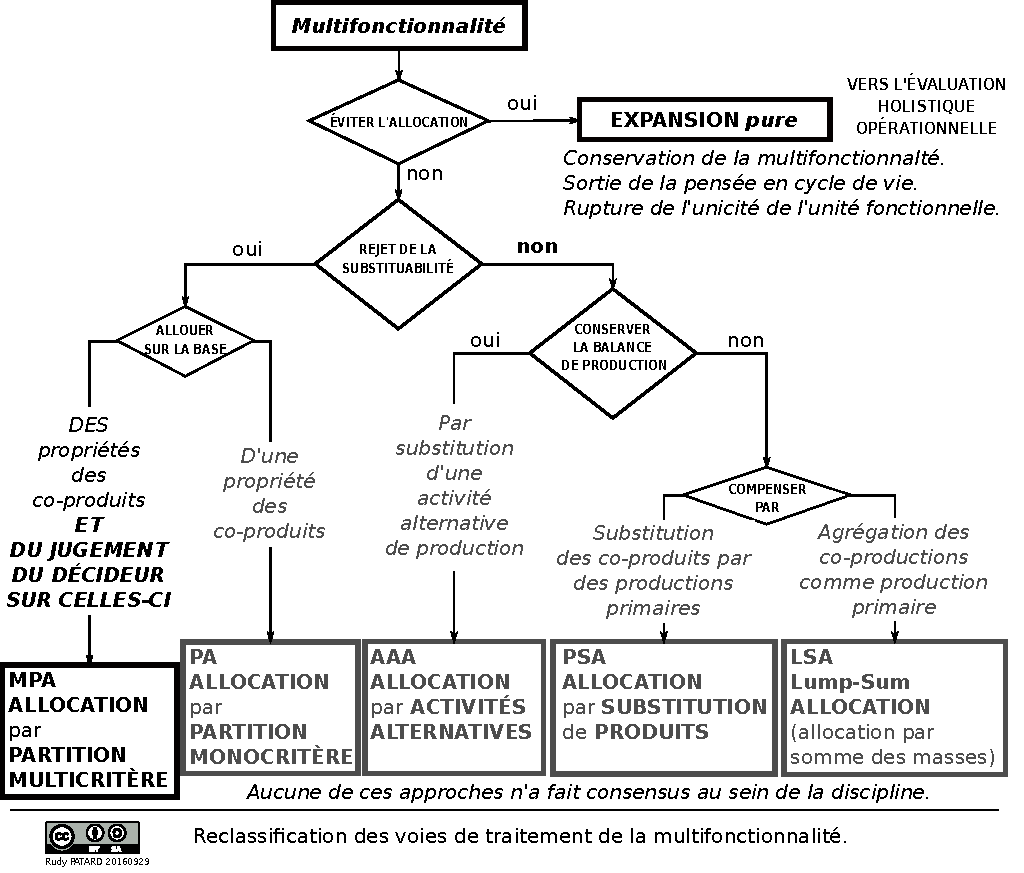
\includegraphics[width=\textwidth]{/home/rudy/Documents/rudy/01_These/11_production/01_COMMUNICATION/figures/allocation/Traitement_de_la_multifonctionnalite_reclassification.pdf}
\caption{Re-classification des approches de résolutions de la multifonctionnalité.}
\label{fig:MULTIFONCTIONNATLITE_REclassification}
\end{figure}
\figbox{
En somme sous le paradigme de l'ACV avec unicité de l'\gls{UF} nous avons deux approches, la partition et la substitution, sous ses diverses variantes, conservatrices ou non de balances de production, LSA, PSA, AAA.
%Dans l'approche par partition l'expansion peut être incluse comme première étape (ordonnancement).
L'ajout de fonctions au modèle nécessite la comparaison d'alternatives répondant à diverses fonctions.
Sous le principe de l’expansion pure, la préférence entre les alternatives socio-techniques est définie entre deux ensembles (fonctions et impacts) de dimensions et quantifications différentes.
L'approche par partition pose le jugement entre fonctions à l'échelle du procédé de premier plan.
Il s'agit du niveau duquel est délivré le flux fonctionnel de référence.
La partition alloue l'inventaire entre les flux fonctionnels issus de l'activité traitée.
Cette méthode permet le traitement de chacune des alternatives socio-techniques observées sans qu'un cas d'étude ne soit non solvable par cette méthode\footnote{Contrairement à l'opposition de produits de substitution, b et b', comme vu plus haut.}.
}

\section{Allocation par partition revisitée}
\label{sec:partitionning}
Nous allons dans cette partie apporter des modifications à l'équation générale de \citeauthor{majeau-bettez_unified_2014}.
Nous présentons tout d'abord l'ajout explicite des préférences.
Après une présentation du modèle nous suivrons sont comportements suivant les domaines parcourus par les propriétés des flux.
Ceci nous amènera à redéfinir le statut du déchets.
Nous dépasserons le statut de déchet économique pour obtenir le déchets économique \textbf{et} \emph{d'usage}.
Ceci nous conduira à réévaluer les frontières des systèmes en responsabilités et en appréciations pour finalement juger de l'importance de l'intention (volonté de création du flux) et de sa destination (son usage effectif).

\subsection{Un modèle d'allocation avec préférences explicites}
Dans la formulation précédente de l'allocation par partition, chaque procédé a \emph{une} et une seule propriété intensive déclarée comme clef d'allocation ($\psi_{iJ}$).
Développer la gamme de propriétés considérées donne un indice additionnel~: $\psi_{niJ}$.
%In the previous formulation each process has \emph{one} intensive property declared as allocation key ($\psi_{iJ}$).
%Developing the range of properties to consider we get an additional indices: $\psi_{niJ}$.
%\footnote{
$n$ sont les indices pour les propriétés des flux fonctionnels produits considérés et $\mathcal{N}$ est le domaine des propriétés, ainsi $n \in \mathcal{N}$.
$N$ est la fraction de $\mathcal{N}$ \emph{concernée par tous les flux des activités} $J$ \emph{étudiés pour l'allocation}.
%$n$ is the indices for the properties of commodities we are considering
%and $\mathcal{N}$ is the domain of properties, so $n \in \mathcal{N}$.
%$N$ is the fraction of $\mathcal{N}$ \emph{concerned by all flows of the activity} $J$ \emph{studied for allocation}.
%}
\footnote{Ceci signifie que pour l'implémentation, le facteur d'importance relative devra être dérivé de chaque procédé appelé pour traitement de multifonctionnalité.}
Le système de préférence est joint au ratio de propriétés dans l'expression des coefficients techniques dans l'équation \eqref{eq:technical_coefficient_multicriteria}.
Le coefficient technique devient ainsi~:
%The preference system is joined to the property ratio in the expression of technical coefficients in the following equation: \eref{eq:technical_coefficient_multicriteria}.
%The technical coefficients thus become:

%\footnote{This means that for implementation, the relative importance factor shall be derived at each process calling for allocation.}
%The preference system is joined to the property ratio in the expression of technical coefficients in the following equation: \eref{eq:technical_coefficient_multicriteria}.
%The technical coefficients thus become:
% Giving as a result the expression of the ``technical requirement matrix'':

%\begin{center}
%\colorbox{yellow}{ Recherche de formulation sur le terme de préférence 
%$\frac{\mathit{Pref}(\psi_{njJ})}{\displaystyle\sum_{n \in N} \mathit{Pref}(\psi_{njJ})}$
%}
%
%ou
%
%\colorbox{yellow}{
%${\mathit{Pref}(\psi_{njJ} / N)}$, moins orienté sur une méthode de dérivation.
%}
%\end{center}

\begin{equation}
  \begin{split}
  & a_{iJk}=u_{iJ}\displaystyle\sum_{n \in N}\dfrac{\psi_{nkJ}}{\displaystyle\sum_{j\in\bullet}\psi_{njJ}v_{jJ}} \mathit{Pref}(\psi_{njJ/N})
  \\
%   &  \forall k|(k,J) \in \mathcal{J},i \in \bullet,J \in \ast, N \in \mathcal{N}
  \end{split}
  \label{eq:technical_coefficient_multicriteria}
\end{equation}
La conservation de la balance globale de production qui résulte de la normalisation aux propriétés présentes et aux préférences respectives est présentée Eq.~\eqref{eq:production_balance}\footnote{Il sera compris qu'ici les pseudo-procédés monofonctionnels non \emph{plus aucune} 'balance' de propriété d'équilibrée, conformément à la description de \citeauthor{weidema_avoiding_2010}.}.
%with the production balance conservation resulting from the normalization to present properties and respective preferences: % in \eref{eq:production_balance}.
%
%$
%1 = \sum_{n,k}\left\{\frac{\psi_{nkJ}v_{jJ}}{\sum_{j\in\bullet}\psi_{njJ}v_{jJ}} \frac{\mathit{Pref}(\psi_{njJ})}{\sum_{n \in N} \mathit{Pref}(\psi_{njJ})} \right\}
%$
%
\begin{equation}
1 = \displaystyle\sum_{n,k}\left\{\frac{\psi_{nkJ}v_{jJ}}{\displaystyle\sum_{j\in\bullet}\psi_{njJ}v_{jJ}} \mathit{Pref}(\psi_{njJ/N}) \right\}
\label{eq:production_balance}
\end{equation}
%
%Thus the distinction between primary, secondary product or elementary flows and product flows are dismissed.

Le formalisme de \citeauthor{majeau-bettez_unified_2014}
\blockcquote[traduction]{majeau-bettez_unified_2014}{
[\ldots] pourrait faire croire que cela limite [le] cadre de répartition des activités dans le cas d'un produit primaire clairement identifiable, mais ce n'est pas le cas.
À ce niveau de généralité, cela signifie simplement que notre description de l'allocation est exprimée en termes d'un produit choisi parmi ses coproduits.
Pour de nombreuses techniques d'allocation, cette sélection peut être complètement arbitraire.
%This nomenclature might make it seem as though this limits our framework to allocation of activities with a clearly identifiable primary product, but it is not the case. At this level of generality, it merely means that our description of allocation is expressed in terms of one product selected among its coproducts. For many allocation techniques, this selection can be completely arbitrary.
}
La distinction entre \emph{primaire} et \emph{secondaire} n'est maintenant plus nécessaire, qu'elle fut arbitraire ou d'une subjectivité collective\footnote{Ce qui pourrait être considéré principal serait le flux recueillant le plus de préférence.}.
Nous pouvons donc passé d'une distinction `arbitraire mais sans conséquence' (apparente), à `évité'.
%The identification of \emph{primary} production is no longer \emph{arbitrary}\footnote{It is the most valued flow according to the decision maker preferences}.
%So we can go from consequence free
%\footnote{
%\blockcquote{majeau-bettez_unified_2014}{This nomenclature might make it seem as though this limits our framework to allocation of activities with a clearly identifiable primary product, but it is not the case. At this level of generality, it merely means that our description of allocation is expressed in
%terms of one product selected among its coproducts. For many allocation techniques, this selection can be completely arbitrary.}
%},
%to avoided.
Éliminer la dualité primaire -- secondaire simplifie également le formalisme de ~\citeauthor{majeau-bettez_unified_2014} et les notations consécutives à la distinction entre primaire et secondaire ($\underline{a}_{iJk}$ ; $\tilde{\underline{A}}$\ldots).

%Clearing the duality primary -- secondary products simplifies \textsc{Majeau-Bettez}~'s work~\cite{majeau-bettez_unified_2014} and notations ($\underline{a}_{iJk}$ ; $\tilde{\underline{A}}$$\ldots$).
Les flux alloués deviennent~:
%The allocated flows become:
\begin{equation}
%\begin{align*}
 z_{iJj}=a_{iJj}v_{jJ}= u_{iJ}\sum_{n,k}\dfrac{\psi_{nkJ}v_{jJ}}{\displaystyle\sum_{j\in\bullet}\psi_{njJ}v_{jJ}}\mathit{Pref}(\psi_{njJ/N})\\
\forall k,i,j \in \bullet | \forall J \in \ast | \forall n \in \mathcal{N}
\label{eq:multicriteria_allocated_flows}
%\end{align*}
%%\begin{align*}
% z_{iJj}=a_{iJj}v_{jJ}= & u_{iJ}\sum_{n,k}\dfrac{\psi_{nkJ}v_{jJ}}{\displaystyle\sum_{j\in\bullet}\psi_{njJ}v_{jJ}}\mathit{Pref}(\psi_{njJ/N})\\
%&\forall k,i,j \in \bullet | \forall J \in \ast | \forall n \in \mathcal{N}
%\label{eq:multicriteria_allocated_flows}
%%\end{align*}
\end{equation}
\figbox{Nous précisons dans l'Eq.\eqref{eq:multicriteria_allocated_flows}, que l'expression du flux alloué vaut quelques soient les commodités, quelques soient les activités et quelques soient les propriétés.}
%

!!! PB avec l'exbox l 1016 à 1077

%\exbox{
%Reprenons notre exemple simple~:\\
%%\newline
%{\scriptsize
%(Rappel) Dans l'activité \textbf{A}, à partir de~:
%\begin{itemize}[noitemsep]
%\item la consommation de 3~l de \textbf{s},
%\item la consommation 1~kWh d'électricité \textbf{f}
%\item l'émission de 10~g de \textbf{x} dans l'air
%\item etc,
%\end{itemize}
%sont conjointement produits~:
%\begin{itemize}
%\item 100 unités de \textbf{a} pour une masse de 2~kg  (0.020~kg/unité) et un prix de 10~k€ (100~€/unité),
%\item 20 unités de \textbf{b'} pour un total de 1~kg (0.05~kg/unité) pour 2~k€ (100~€/unité).
%\end{itemize} 
%
%L'inventaire de l'activité A (les 3~l de \textbf{s}, le kWh d'électricité \textbf{f}, l'émission de 10~g de \textbf{x} dans l'air etc) était réparti~:
%\begin{itemize}[noitemsep]
%\item à 2/3 pour \textbf{a} et 1/3 pour \textbf{b'} suivant une clef massique.
%\item à 5/6 pour \textbf{a} et 1/6 pour \textbf{b'} suivant une clef monétaire.
%\end{itemize} 
%}
%La préférence entre une valorisation monétaire et une valorisation massique est définie par le décideur fictif à~:
%\begin{center}
%$
%\begin{matrix}
%	& masse & prix & Priorité \\
%masse & 1 & 1/4 & 0.2 \\
%prix & 4 & 1 & 0.8 \\
%\end{matrix}
%$
%\end{center}
%
%Voyons comment est maintenant produite l'allocation, \emph{en suivant le formalisme présenté}.
%Le flux d'électricité \textbf{f}, alloué à la production de \textbf{a} dans l'activité A, c'est à dire $z_{fAa}$ est tel que~:\\
%%\footnote{Le développement est présenté avec l'information dimensionnelle. N signifie Nombre d'Unité Produite.
%%Bien que sans dimension nous pensons que ces 'quantité d'item' aiderons la lecture.}
%%}
%
%{\small
%\begin{equation}
%\begin{align*}
%z_{fAa} = & u_{fA}(\\
%&\frac{\mathit{masse_{aA}/N_{aA}}}{(\mathit{masse_{b'A}/N_{b'A}}) \mathit{N}_{b'A} + (\mathit{masse_{aA}/N_{aA}})\mathit{N}_{aA}} \mathit{N}_{aA} \mathit{Pref}(\psi_{\mathit{masse} aA/N})\\
%&+\frac{\mathit{prix_{aA}/N_{b'A}}}{(\mathit{prix_{aA}/N_{b'A}}) \mathit{N}_{b'A} + (\mathit{prix_{aA}/N_{aA}})\mathit{N}_{aA}}  \mathit{N}_{aA}  \mathit{Pref}(\psi_{\mathit{prix} aA/N}))\\
%z_{fAa} = & 1(kWh)(\\
%&\frac{0.02(kg/N_{aA})}{0.05(kg/N)20(N_{b'A}) + 0.02(kg/N_{aA})100 (N_{aA})} 100 (N_{aA}) 0.2\\
%&+\frac{100(\geneuro/N)}{100(\geneuro/N)20(N_{b'A}) + 100(\geneuro/N)100 (N_{aA})})  100 (N_{aA}) 0.8\\
%z_{fAa} = & 2/3 \times 0.2 + 5/6 \times 0.8 = 0.8
%\end{align*}
%\end{equation}
%}
%Ceci se lie beaucoup plus aisément que dans le formalisme initiale de \citeauthor{majeau-bettez_unified_2014}.
%Il n'y a plus de soustraction au primaire par le secondaire.
%Il s'agit simplement de multiplier, le ratio de propriété par le ratio de préférence relative de la propriété.
%
%La vérification, ici aisée pour $z_{fAb'} = 1/3 \times 1/5 + 1/6 \times 4/5 = 0.2$ confirme l'expression de l'Eq.~\eqref{eq:production_balance}.
%
%Nous pouvons faire remarquer au passage l'indépendance à l'unité.
%Si plutôt que l'euro nous prenons le k\geneuro, le ratio des prix reste identique par l'emploi de la propriété intensive du prix (/unité)\footnote{Prendre la température des produits a et b ne fonctionnerait pas.}.
%}

\subsection{Comportement du modèle}


%Mettre la figure coproduction - cotraitement à la place
%\begin{figure*}
%
%\centering
%\resizebox{1.00\textwidth}{!}{
%%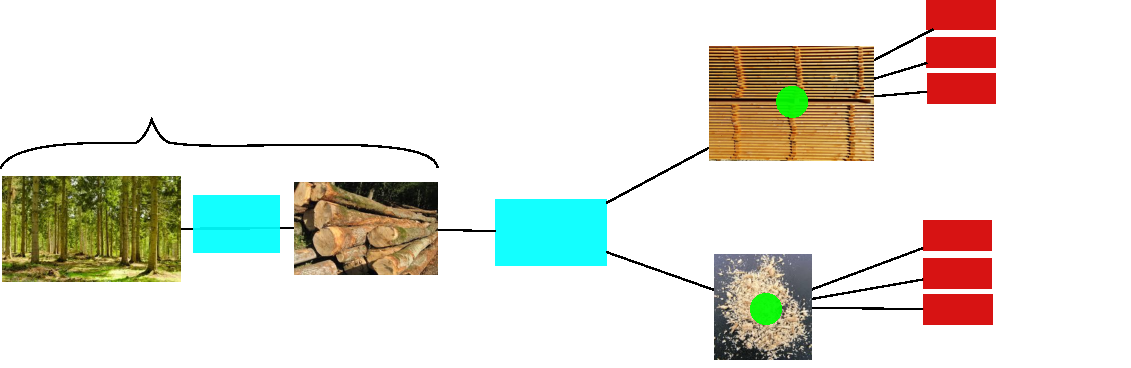
\includegraphics{/home/rudy/Documents/rudy/01_These/11_production/01_COMMUNICATION/figures/alloc_value_integrated_20160226.pdf_tex}
%\input{/home/rudy/Documents/rudy/01_These/11_production/01_COMMUNICATION/figures/alloc_value_integrated_20160226.pdf_tex}
%}
%% à remettre dans le .pdf_tex après modif : /home/rudy/Documents/rudy/01_These/11_production/01_COMMUNICATION/figures/
%\caption{A process chain schema to introduce allocation treatment with multiple allocation keys possible. Commodity "l" bears the attributes a, b, c in the respective shares $\alpha$, $\beta$ and $\delta$.}
%\label{fig:alloc_example}
%\end{figure*}


%
%
%The allocation factors then are:
%\begin{equation}
%a_{iBl} = \dfrac{\alpha}{\alpha+\lambda} a * \frac{\mathit{Pref}a}{\displaystyle\sum_{i = a}^{c} \mathit{Pref}i}+ \dfrac{\beta}{\beta+\gamma} b * \frac{\mathit{Pref}b}{\displaystyle\sum_{i = a}^{c} \mathit{Pref}i}+ \dfrac{\delta}{\delta+\nu} c * \frac{\mathit{Pref}c}{\displaystyle\sum_{i = a}^{c} \mathit{Pref}i}
%\end{equation}
%
%\begin{equation}
%a_{iBm} = \dfrac{\lambda}{\alpha+\lambda} a * \frac{\mathit{Pref}a}{\displaystyle\sum_{i = a}^{c} \mathit{Pref}i}+\dfrac{\gamma}{\beta+\gamma} b * \frac{\mathit{Pref}b}{\displaystyle\sum_{i = a}^{c} \mathit{Pref}i}+\dfrac{\nu}{\delta+\nu} c * \frac{\mathit{Pref}c}{\displaystyle\sum_{i = a}^{c} \mathit{Pref}i}
%\end{equation}

Nous proposons l'utilisation de la méthode du processus analytique de hiérarchisation (AHP)~\cite{saaty_decision_2004} pour la dérivation des préférences entre les clefs d'allocation.
La technique est détaillée dans la chapitre relatif à la décision multi-critère au~\ref{subsubsec:AHP}.

%We propose to use \textsc{Saaty}'s method Analytical Hierarchy Process (AHP)~\cite{saaty_decision_2004} for deriving relative priorities among allocation keys.
%? Est-ce que l'on garde la matrice ?
La matrice de comparaison par paires est donnée sous la forme suivante~\eqref{pair-wise matrix}.
%The pair-wise comparison matrix is as follow
\begin{equation}
\begin{matrix}
	& \psi_{a} & \psi_{b} & \psi_{c} \\
\psi_{a} & ^{W_a}/_{W_a} & ^{W_a}/_{W_b} & ^{W_a}/_{W_c} \\
\psi_{b} & ^{W_b}/_{W_a} & ^{W_b}/_{W_b} & ^{W_b}/_{W_c} \\
\psi_{c} & ^{W_c}/_{W_a} & ^{W_c}/_{W_b} & ^{W_c}/_{W_c} \\
\end{matrix}
\label{pair-wise matrix}
\end{equation}


%
%	& \psi_{a} & \psi_{b} & \psi_{c} \\
%\psi_{a} & ^{W_a}/_{W_a} & \frac{W_a}{W_b} & \frac{W_a}{W_c} \\
%\psi_{b} & \frac{W_b}{W_a} & \frac{W_b}{W_b} & \frac{W_b}{W_c} \\
%\psi_{c} & \frac{W_c}{W_a} & \frac{W_c}{W_b} & \frac{W_c}{W_c} \\

Les termes du vecteur de priorité est donnés par
$\mathit{Pref}(\psi_{njJ/N})$.
%The $\frac{\mathit{Pref}a}{\sum_{i = a}^{c} \mathit{Pref}i}$ are the terms of the priority vector.
Ils pourraient être exprimés par la moyenne géométrique~:
$		{p_i}=\displaystyle\frac{\sqrt[n]{\prod_{j=1}^{n}{A_{1j}}}}{\sum_{i=1}^{n}\sqrt[n]{(\prod_{j=1}^{n}{A_{1j}})}}
$\footnote{Même si \citeauthor{saaty_making_2005} la rejette~\cite[6. Non-additive Synthesis-Why the Geometric Mean Does not Work]{saaty_making_2005} (\textit{cf.} sec.~\ref{subsubsec:AHP}.}.

%\colorbox{yellow}{reprendre la notation avec un symbole pour la préférence relative autre que la formule par somme pour ne pas orienter sur une méthode de dérivation des priorités particulière.}
Comme indiqué précédemment, il y a diverse méthodes de dérivation~\cite{ishizaka_how_2006}
\footnote{
Ceux souhaitant tester différentes alternatives (vecteur propre, moyenne normalisée, moyenne géométrique) peuvent utiliser le paquet logiciel existant~\cite{glur_ahp_2016}.
}
%There are multiple priority derivation techniques~\cite{ishizaka_how_2006}\footnote{
%Those willing to test different alternatives (eigenvalues, mean normalization, geometric mean) can use existing packages~\cite{glur_ahp:_2016}.}

\exbox{
Dans un exemple blanc, nous considérons le cas décrit dans la table~\ref{tab:exemple_3_attributs}.
Les attributs choisis pour l'exemple reprennent les clefs courantes (monétaire, massique, énergétique).}
%In the blank example below we can consider the following case.
\begin{table}[h]
  \begin{center}  
  \begin{tabular}{| c|c |c |c |c|}
  \hline
 & EUR & kWh & kg & Priorité \\ 
 \hline
EUR & 1     & 6     & 4     & 0,70 \\ 
kWh &  1/6 & 1     &  1/3 & 0,09 \\ 
kg &  1/3 & 2     & 1     & 0,21 \\ 
  \hline
  \end{tabular}
  \end{center}
    \caption{Matrice de comparaison par paires, visant des attributs de flux, remplie à titre d'exemple.}
  \label{tab:exemple_3_attributs}
  \end{table}

La hiérarchie ne porte pas sur les intensités mais les valeurs en jeux.
Nous employons en allocation par partition des attributs, des propriétés intensives.
La multiplication des termes de quantification des flux nous donne la mesure de l'attribut~\cite{majeau-bettez_unified_2014}
\footnote{$(\mathit{masse}~/~\mathit{unité})\times\mathit{nombre~d'unité(s)}$ comme vue lors de l'exemple précédent en PA standard.}.
%Hierarchies is not about intensity.
%We use intensive attribute in partitioning, as advocated by \textsc{Majeau-Bettez}~\cite{majeau-bettez_unified_2014} because the multiplication with the flow quantification brings us the value.
%\begin{table}
%  \begin{center}
%  \caption{Valeurs et propriétés intensives pour la partition}
%%  \tbl{}{
%  \begin{tabular}{| p{0.3\textwidth} | p{0.3\textwidth} | p{0.3\textwidth} |}
%  \hline
%	Intensive properties & price (EUR/unit ; EUR/kg) & calorific value (J/unit ; J/kg ; J/mol) \\ 
%	\hline
%	Values & exchange (monetary) values & Energy value \\
%  \hline
%  \end{tabular}
%%  }
%  \end{center}
%  \label{tab:Valeurs et propriétés intensives pour la partition}
%  \end{table}

%\begin{center}
%\colorbox{yellow}{Commentaire perdu : à resituer, peut-être section indicateurs}
%\end{center}
Nous pourrions discuter que l'énergie est une sorte d'échange de travail.
Et les échanges en seraient caractérisés comme avec des devises sans spécification que le travail soit fourni par des hommes.
Les différences de classification et d'interprétation des indicateurs pourraient conduire à des vecteurs de priorités différents.
Il est donc important de ne pas négliger dans les cas réel cette 'architecture des valeurs', ce que nous appelons la réflexion axiologique.
%One could for instance argue that energy is some trade of work and exchanges of exergy are located in exchanges values without the specification that the work is provided trough humans as in a currency.

Nous poursuivons l'application fictive à une séries de cas donnés table~\ref{tab:allocation_partition_cas_dissociable}.
%\resizebox{\linewidth}{
\begin{table}[h!]
  \begin{center}
%  \tbl{}{
\resizebox{\textwidth}{!}{
  \begin{tabular}{|| l||c |c |c ||c |c |c ||c ||c ||c}
  \hline
  & \multicolumn{3}{ c|| }{PRODUIT 1} & \multicolumn{3}{ c|| }{PRODUIT 2} & \multicolumn{2}{ c|| }{Allocation} \\
%   & PRODUCT 1 &  &  & PRODUCT 2 &  &  & Scale AHP &  & \\
  \hline
  Cas & EUR & kWh & kg & EUR & kWh & kg & PDT 1 & PDT 2 \\
  \hline
  a & 2 & 6 & 15 & 8 & 7 &  & 39,3\% & 60,7\% \\
  b &  & 102 & 56 & 24 & 15 & 33 & 21,3\% & 78,7\% \\
  c & 13 &  & 32 & 25 & 16 & 19 & 37,1\% & 62,9\% \\
  d & 14 & 104 &  &  & 17 & 12 & 77,6\% & 22,4\% \\
  e & 10 & 100 & 11 & 22 &  & 27 & 37,1\% & 62,9\% \\
  \hline
  \hline
  dissocié & 10 &  & 25 &  & 13 &  & 90,8\% & 9,2\% \\
  \hline
  \end{tabular}
  }
  \end{center}
  \caption{Allocation par partition, différents cas fictifs de l'hétérogénéité à l'incommensurabilité.}
  \label{tab:allocation_partition_cas_dissociable}
  \end{table}
%  }
\figbox{
Dans la table~\ref{tab:allocation_partition_cas_dissociable} sont présentés différents cas.
Quelque soit le manque de donnée, la balance globale de production est respectée.
%What ever the lack in data, the production balance remains.
\emph{Il est même possible, tel que souligné dans le cas "dissocié" que des co-productions de natures et donc de propriétés tout à fait différentes soit utilisées en partition}.
}
%It is even possible as stressed out by the "dissociate" line that \emph{co-product of completely different attribute be used in partitioning}.
Il ne s'agit pas ici des balances locales (sous-procédé), mais de la balance globale.
Toutes les balances individuelles sur les propriétés sont perturbées bien entendu.
Nous n'en sommes plus au stade de la description, nous avons déjà intégrer l'évaluation.

Le fonctionnement même en présence de manque de données peut être jugé comme une bonne chose (robustesse).
Il implique cependant la nécessité d'un mécanisme de contrôle et d'avertissement du décideur.
Par exemple, l’interruption et l'alerte pour l'absence de données spécifiques ou un affichage préalable avant l'indication de la solution 'préférée' du taux de présence ou d’absence par types de données.

\subsection{Cas particuliers}

\subsubsection{Attributs négatifs}
Lorsque l'on emploie une valeur monétaire pour caractériser un flux (réification du prix, transformation de la propriété d'un échange en 'prix de l'objet'), si la préférence sur l'indicateur monétaire est suffisante, cela génère une part négative de l'inventaire pour le flux "payé".

%When using monetary value as an attribute of the flow, if the preference toward monetary value is sufficient, it enable negative share of inventory for the "paid flow".

\begin{table}[h!]
%  \begin{center}
%    {
	  \begin{tabular}{|c|c|c|c|c|c|c|c|c|c|c|}
	  \hline
	  & \multicolumn{3}{ c| }{PRODUCT 1} & \multicolumn{3}{ c| }{PRODUCT 2} & \multicolumn{3}{ c| }{Scale AHP} \\
	  \hline
	  Test& EUR & kWh & kg & EUR & kWh & kg & PDT1\% & PDT2\% & Balance \\
	  \hline
		A& -25& 10& 32& 25& 16& 19&\#DIV/0\! &\#DIV/0\! &\#DIV/0\! \\ 
		B& -8& 10& 32& 25& 16& 19& -16,0\% & 116,0\% & 100\% \\ 
		C& -4& 10& 32& 25& 16& 19& 3,5\% & 96,5\% & 100\% \\
		D& -60&	10&	32&	25&	16&	19&	136,2\%& -36,2\%& 100\% \\
		
\hline
\end{tabular}
%	      \caption{Here are presented different special cases.\\
%	      	    A: "Nullified" attributes, \\
%	      	    B: "Waste" ? negative monetary values,\\
%	      	    C: "Wasted" ? monetary undervalued use values.\\
%	      	    D: in deficit activity.}
%	}
%	\begin{tabnote}
\caption{Cas limites induits par des valorisation négatives.}
%	\end{tabnote}
%  \end{center}
\label{tab:attributs négatifs}
  \end{table}

\figbox{
Dans la table~\ref{tab:attributs négatifs}, nous pouvons voir différentes configurations déclenchant divers effets sur le modèle d'allocation.
%Here we can see different configuration triggering effect on the allocation model.
Les cas sont les suivants~:\\
 A: "Nullified" attributes, équilibrés ou annulés \\
 B: "Waste" ? negative monetary values, une valeur monétaire et globale négative \\
 C: "Wasted" ? monetary undervalued use values, une valeur monétaire négative mais globalement positive \\
 D: in deficit activity, une activité déficitaire avec valeur \emph{ajoutée} observable.


Premièrement, observons le cas de l'annulation ou plutôt d'équilibrage de valeurs.
Il apparaît lorsque sur les différents flux appréciés ils s'en trouvent des négatifs compensant les positifs.
%Firstly, we shall see nullified valuations.
%It appears when on the different co-products, one attribute gives a null sum.
La racine du phénomène découle du dénominateur de du coefficient technique, cf Eq.~\ref{eq:technical_requirement_coefficient_majeau}
%The root comes from the denominator in equation \eqref{eq:technical_requirement_coefficient_majeau}
 $\sum_{j\in\bullet}\psi_{jJ}v_{jJ}$.
 
Sur la condition nulle et ses voisins, l'allocation par partition échoue (théoriquement division par zéro), ou donne (plus vraisemblablement) des résultats erratiques jusqu'à des milliers de pourcentages (par soucis de lisibilité limités à la dizaine ici).
%On the null condition and on limits bordering null condition, the allocation either fails (by zero division) or gives aberrant results (thousands of \% shares).

Le cas B est une perception assez juste (à première vu) du déchet.
Toujours par effet du dénominateur, nous avons ici des attributs appréciés (positivement), qui ne contre balance pas le \textit{coût} monétaire du flux.
C'est donc que l'échange satisfait d'autr(e) besoin(s) que la possession positive du flux (encombrement, gêne, dangerosité, conformité réglementaire).
Ceci peut souligner le manque d'envergure d'une matrice de jugement (assez simple à produire à seulement 3 dimensions).

Dans le cas C, les valeurs d'usages contre-balancent le coût monétaire.
Le possesseur ou propriétaire (par obligation ou ignorance) se défait d'un flux en le payant au possesseur successif.
De nombreux modèles d'\textit{écologie industrielle} ou d'\textit{économie bleu}, reposent sur ce principe.
Les selles que je produits pourraient m’être utile pour mon potager.
Mais inadéquatement localisé en ville, je paie pour l'enlèvement de cette riche matière organique et les micro-organismes qui l'accompagnent.

}

Avec la réification passant de la propriété du flux à celle de l'objet, nous \textit{permettons} une "mesure négative".
%With reificitation granting the monetary attribute a property to the flow and not the exchange process between human beings, we allow negative "measures".
Ce n'est pas la spécialité de l'allocation multicritère.
Si la méthode suivie est la partition et que la clef d'allocation est économique, ceci peut être une occurrence de l'allocation mono-critère.
C'est pour cette raison que les principes d'allocation actuels requièrent la distinction entre "déchet" et "produit" sur la base de leur valeur marchande.
%This is no speciality of multi-criteria allocation.
%If partitioning follow price as an intensive property, this would mean these case could exist with current mono-dimension partitioning.
%Of course excluding "waste" of "co-production" treatment "solves" the question.
Mais c'est encore ici faire le monopole de la valeur économique dans le champ \emph{des} valeurs, dans le champ de la richesse.
La question de la détermination du statut du flux reste donc à traiter.
%But the question remains to determine flow status.

La nuance porte sur \emph{quand}, à quel seuil, mettre un flux sous le statut de produit.
Où se trouve la définition d'un flux apprécié positivement.
Nous allons le voir sur les différents cas observés.
%The nuance is WHEN to put a flow under "product" status.
%Where is the definition of a valued flow?
%We'll see to it is cases observation.

Pris en isolation, le flux apprécié négativement générerait un inventaire négatif.
Qualifier une émission de négative sans qu'il y ait dans les faits une absorption est difficilement tolérable scientifiquement.
Nous n'avons rencontré ce phénomène qu'avec l'emploi du coût pour des co-productions qualifiées de déchets.
Mais en plongeant dans cette perspective d'intégrer une matrice de jugement complète sur l'ensemble des étapes de l'ACV, l'inclusion des impacts a levé de nouveaux items.
Qu'en est-il des attributs considérés négativement lorsqu'ils accompagnent des attributs jugés positifs~?
D'autres points d'équilibres pourraient être trouvé et c'est ce qui nous amène à la généralisation de ces cas particuliers.
%Taken in isolation, negatively valued flow would generate negative inventory for the production of this entity.
%It cannot be scientifically accepted.
%Reification would seems to invalidate the proposed partitioning system (in the proposed model as in previous mono-criterion form).
%With the cases below we will define scope in which the allocation model remains acceptable".
%We came across this issue only with monetary attribute with allocation.
%But diving into perspectives of integrating a full judgement matrix for all LCA modelling decision and \emph{including impacts} quickly rises new items.
%What on negatively perceived attributes?
\subsubsection{Co-systèmes et co-traitements}
Considérons maintenant dans un second cas que les "sorties" négatives sont du domaine de la responsabilité.
Un flux apprécié négativement, qui générerait une part négative de l'inventaire devrait être considéré de la responsabilité de l'activité d'origine.
Il devrait être intégré au modèle, non pas en co-production mais en co-système (délivrant les flux appréciés positivement).
Les flux valorisés (en usage comme en échange) en sortie du co-système seraient traités en partition de la même façon.
C'est actuellement ce qui découle de la procédure en deux étapes d'allocation de l'ILCD.
\blockcquote[traduction p~352-353]{european_commission_ilcd_2010}{
On fait valoir que tous les processus de traitement qui sont nécessaires jusqu'à ce que les déchets traités / produits en fin de vie, aient obtenu une valeur de marché de zéro sont sous la responsabilité du premier système.
%It is argued that all treatment processes that are necessary until the treated waste / end-of-life product is achieving a market value of zero are within the responsibility of the first system.
}

Nous retrouvons donc les principes actuels de la communauté scientifique, mais la distinction de statut déchet/produit, comme l'ensemble des jugements lors de l'allocation, serait le résultat de la matrice des jugements explicités.
Il n'y aurait plus de 'dictât' de la valeur économique.
%Negative outputs are the domain of responsibilities.
%A negative outputs that generate negative share of inventory should be considered of full responsibility of the originating activity and should be integrated into the model, not for co-production but as co-system.
%Positively valued output of the co-system would then be treated by the same partitioning method.

Il y a quelques répercussions consécutives intéressantes à observer sur la considération de l'attribut économique tout de même.
Ici nous allons développer l'importance de fusionner la matrice de jugement pour la construction de l'inventaire comme pour l'interprétation des impacts.
%There are some following interesting consequences.
%And here we will develop the importance of merging allocation judgement matrix and impact interpretation matrix.
Avec la part négative de l'inventaire, une relation particulière est créée entre les produits et leur déchets.
Le fardeau est en effet porté par les produits, les flux valorisés, portant (en considérant les plus isolément) plus de $100 \%$ de la charge totale.
%With negative share of inventory, a particular relation is created between the products and waste. 
%The burden is indeed supported by the valued products (taking more than 100~\% of the "load").
Pour la chaîne de traitement, s'ils annulent leurs impacts (au sens de la compensation de leur propres impacts du fait de leur émissions et consommation, par la valeur négative entrante), alors ils auront équilibré les problèmes environnementaux contre lesquels sont payés leurs services.
%For the treatment chain, if they nullify their impact (meaning entering with negative impacts products and adding their positive impacts), then they balance the issues of a products they are paid to "treat" as an environmental issue.
Si leur impact reste positif, cela indique que la performance de traitement est insuffisante et que la tâche est plus vaste et nécessite un engagement de ressources plus important (un plus grand coût), de la part du fournisseur du "déchet".
%If their impact is still positive, this mean they should perform more treatment tasks and then require more expenses so a greater cost to the supplier of the waste.

Pour éviter les résultats d'inventaires négatifs il nous faut intégrer la filière de traitement au système étudié (construire le co-système).
La question prend de l'intérêt lorsque l'on considère les procédés de traitement gérant plusieurs entrées.
Ceci est appelé par \citeauthor{schneider_analyse_1998} "co-traitement"~\cite{schneider_analyse_1998}.

%To avoid resulting negative output with negative inventory we have to integrate the treatment route to the studied system (build the co-system).
%But where it gets interesting is when we acknowledge the co-system.
%The treatment process may handle multiple input.
%This is called by Schneider co-treatment~\cite{schneider_analyse_1998}.


Souvent ces procédés sont modélisés sans leur spectre fonctionnel complet.
Chaleur et électricité sont observées lorsque produites.
Les méthodes d'allocation des déchets prennent déjà en compte ces cas de figures \cite[p.~352, 14.4.1.3 en référence à l' ISO 14044:2006 chapter 4.3.4.3]{european_commission_ilcd_2010}.
Si un flux de matière résultant peut être employé cela est discuté (quel produit va-t-il concurrencer et remplacer et pour quel production évitée...).
Mais la fonction implicite du traitement du flux de déchets est insuffisamment documentée.

\begin{figure}
\centering
%\resizebox{1.00\textwidth}{!}{
%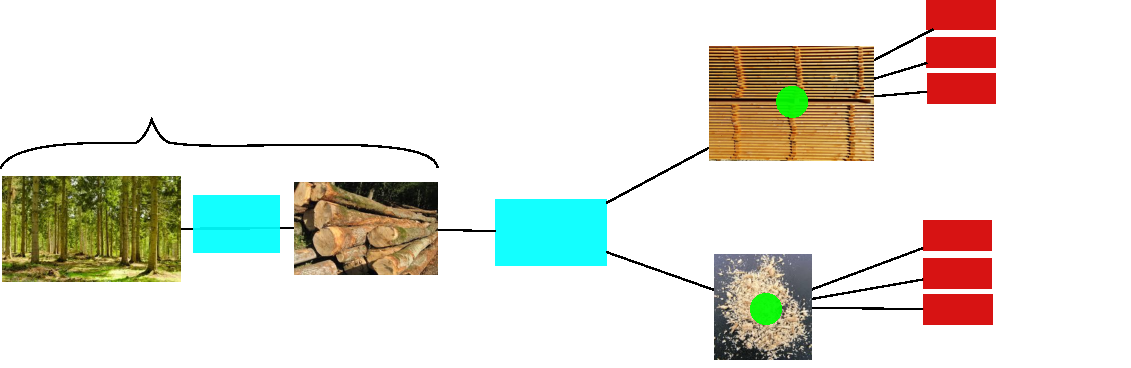
\includegraphics{/home/rudy/Documents/rudy/01_These/11_production/01_COMMUNICATION/figures/alloc_value_integrated_20160226.pdf_tex}
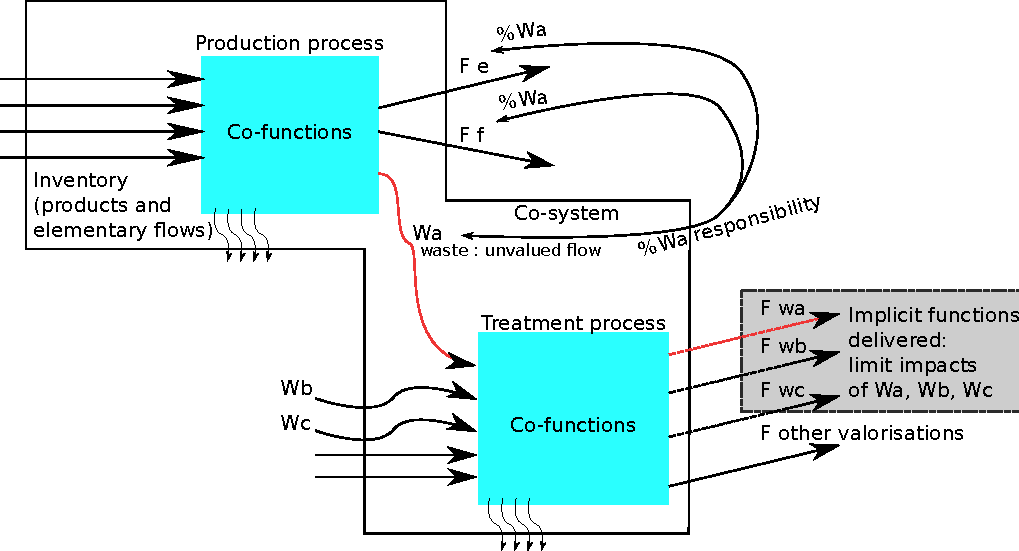
\includegraphics[width=\textwidth]{/home/rudy/Documents/rudy/01_These/11_production/01_COMMUNICATION/figures/co-treatment.pdf}
%}
% à remettre dans le .pdf_tex après modif : /home/rudy/Documents/rudy/01_These/11_production/01_COMMUNICATION/figures/
\caption{Une chaine de valeur introduisant l'allocation avec co-traitement et ses fonctions implicites.}
\label{fig:alloc_co-treatment}
\end{figure}
\figbox{
Dans la figure suivante (\ref{fig:alloc_co-treatment}), nous proposons d'associer la filière et le flux négativement apprécié.
%Often those process are modelled without their full functional spectrum.
%Heat or electricity production is observed.
%If any material flow can be used it is discussed (what substitution can be considered and so on).
%But implicit functions of treating the input flows are insufficiently documented.
%In the following figure, we propose to associate the treatment route to negatively valued flows.

L'allocation entre les flux co-traités peut être déterminée par leur part respective d'impacts calculés dans le cas d'une émission à la biosphère et suivant la matrice de jugement du décideur.
Plus le flux non traité aurait été jugé problématique, plus sa part d'inventaire est importante.
Ceci, pour le co-traitement, suit le même processus d'évaluation que pour les attributs des coproductions classiques.
%The allocation between co-treated flows can be elicited by their share of respective impacts \emph{if} they were released directly in nature \emph{and} following the decision maker judgement matrix. % ! précision sur le rejet à la biosphère sinon -> la poule et l'oeuf
%The more the flow would have been an environmental issue, the more its inventory is important.
%This is done following the same process as evaluating attributes of co-products.

Ainsi l'inventaire alloué de la fonction délivrée $F_e$ est l'allocation des coproductions avec $F_f$ et sa part de l'inventaire pour sa part respective de fonction $F_{Wa}$.
La part $W_a$ décharge l'excédent au dessus des 100~\% de l'inventaire initial et ajoute son propre inventaire pour $F_{Wa}$.
%So the allocated inventory of delivered function $F_e$ is the allocation of the co-production with $F_f$ and its share of inventory for its respective share of function $F_{Wa}$.
%$W_a$'s share unburden the excess above 100~\% of the inventory and its own inventory for $F_{Wa}$ adds up
}

%\begin{figure}
%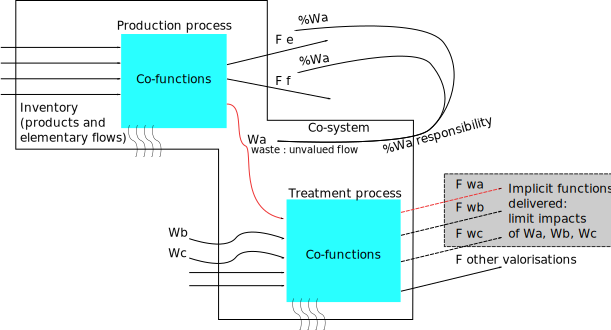
\psfig{file=/home/rudy/Documents/rudy/01_These/11_production/01_COMMUNICATION/figures/co-treatment.pdf_tex,width=4.5in}
%\caption{A process chain schema to introduce allocation with co-treatment case.}
%\label{aba:alloc_co-treatment}
%\end{figure}

%?
%This would remain simple if the value systems were stable and consistent.
%But they are nothing of the sort.
%The range of derivation techniques do not gives a unique solution.
%
%? DVP outranking ?
%So we propose to treat selection of alternative scenario after the LCIA results trough the highest frequency of preference.

%\subsubsection{A monte-carlo based preference}
%
%Based on multiple value judgement matrix, we could repeat LCA's calculation and depict the frequency at which the alternative is prefered.
%To reduce the number of calculation loops, the inconsistent terms on their respective side of the matrix's diagonal would be selected on the difference of their inverse.
%This way we could calculate the results on strongest value contradiction.
%Thus saving calculation times, we could more quickly see the preference divergence.
%On top of inconsistencies from human judgements, a sensitivity analysis shall be conducted in order to pinpoint the strongest link between the value matrix and the modeled system.

%\colorbox{yellow}{TRANSLATION INCOMMING}
Cette proposition, pour être employée, requière que les propriétés et destinations des flux et fonctions soient étudiées.
Ceci appelle au lien entre \gls{ACV} et \gls{MFA}, un courant déjà en marche dans la discipline~\cite{pauliuk_lifting_2015}.
\emph{Mais plus que la traçabilité des produits et substance (MFA actuel), il s'agit ici de réaliser la traçabilité des propriétés, de la façon dont elles sont délivrées et appréciées.}
\exbox{
Par exemple, la masse est habituellement employée pour révélée la quantité de matière, mais elle n'est pas nécessairement la propriété faisant l'intérêt de l'objet.

Du point de vue de la conception industrielle, nos besoins portent plus généralement sur des \emph{surfaces fonctionnelles}.
Remplir de matière pour supporter les contraintes entre ces surfaces nécessite un volume.
Le matériau choisi, répondant adéquatement aux contraintes et porteur d'une certaine densité \emph{implique} donc une masse.
%This proposal, to be used, requests that use properties and destinations be studied.
%This calls for linking LCA to MFA, actually "Lifting Industrial Ecology Modeling to a New Level of Quality and Transparency"~\cite{pauliuk_lifting_2015}.
%But not only tracking products and substances (MFA), doing so means tracking the use properties and how they are delivered and valued.
%For instance, mass is usually used to reveal an amount of material, but it is not necessarily the property that is of interest.
%From design and engineering perspective I'd say we usually need surfaces (functional ones).
%Filling material to support strains between these functional surfaces is the needed volume.
%The material that reply adequately to constraints bearing a density properties comes with a mass.

En nutrition, (pour la flore comme la faune), ce qui est recherché n'est pas une masse de nourriture mais une quantité d'énergie (kcal sur nos emballages), la présence de certains acides aminés et autres.
Ainsi dans ces cas la masse n'est qu'une conséquence de la recherche d'autres propriétés.
%In nutrition (human, animal or plant) what is sought is not the general mass of food, but to provide an amount in energy (kcal), and content in amino acids and else.
%So in those two case, mass would simply be a consequence not a requirement.

Plus occasionnellement la masse fournie une inertie et permet par gravité de garder des choses en place.
Ou encore pour un usage marketing, la masse est employée avec un discours 'lourd=robuste'.
%More occasionally mass is used to provide inertia or kip things in place or as marketing in "heavy = robust" discourses.

Comme il s'agit d'une façon pratique de gérer des quantités de produits délivrant d'autres propriétés appréciées, nous avons tendance à réduire notre intérêt et nos recherches à la seule masse des produits.
%As it is an easy way to handle the amounts of the products that deliver all these properties of interest, we tend to reduce requests and research to a mass of a specific product.
Il nous faut développer le spectre de propriétés de nos investigations.
%We have to develop the property spectrum of our investigations.
}
\subsection{L'intention et la destination}
Le système d'allocation multicritère diffère de la solution existante car il permet la réalisation d'une partition sur la base de co-fonctionnalités totalement hétérogènes.
De plus elle porte dans son principe l'expression explicite des jugements de valeur nécessaires à la distinction entre observations factuelles -- domaine objectif -- et le jugement moral -- domaine subjectif.
%Our multi-criteria system in opposition to prior methods enabled heterogeneous co-products to support partitioning with explicit priorities on values.
Cette nouvelle méthode ouvre des perspectives de valeurs en rendant la distinction initiale entre primaire et secondaire inutile.
Cela permet le traitement en plaine lumière de deux autres enjeux interconnectés, l'intention et la destination.
%However two linked points need digging in the matter of allocation --
%intention and actual use.

\textsc{Weidema} relève une distinction faite la génération précédente par Huppes (1992)~\cite{weidema_avoiding_2000}, une cause probable de problèmes dans la norme ISO et les guides attentant.
Il déclare que
\blockcquote[traduction]{weidema_has_2014}{la hiérarchie de l'allocation pourrait être significativement simplifiée si une séparation était faite entre les cas de coproduction avec une relation variable entre les coproduits et les situations de productions jointes par des relations fixes.}

Si nous écartons le cas ou des relations indépendantes peuvent être établie entre des coproductions et les paramètres d'entrées (c'est à dire une subdivision déguisée), que reste-t-il de l'argument~?~:
Le fait qu'une volonté puisse modifier les `points de fonctionnement' du système.

%\footnote{
%\blockcquote{weidema_avoiding_2000}{An important distinction must be made between joint production, in which the relative output volume of the co-products is fixed, and combined production, with independently variable output volumes (Huppes 1992)}
%}.

%L'argument est que le co-produit utilisé dans le système étudié sera consommé depuis ce procédés à relation variable.
%L'accroissement de quantité produite du fait de la variabilité serait donc équilibré avec ladite consommation\footnote{
%\blockcquote{weidema_avoiding_2000}{For the latter type of production, allocation can be avoided simply by modeling directly the consequences of a change in the output of the co-product of interest (that which is used in the product system under study) without change in the output of the other co-products. This situation is dealt with in step 1 of the procedure.}
%}
%Nous relevons toutefois que si la relation est variable ne pas changer le volume de production des autres coproduits de ce procédé équivaut à un accroissement de l'activité (procédé).
%C'est avec l'hypothèse d'élasticité des prix nulle, une hypothèse additionnelle... où finalement la critique de l'\textit{arbitraire} partition (qui en fait devrait dire subjectif) pourrait se voir opposer l'arbitraire projection économique.

La question que nous soulevons est la suivante~: En quoi le fait qu'une personne puisse interagir avec les parts des différentes productions modifie les propriétés d'usage ou d'échange des flux produits~?
%The intent and application case in allocation.
%\textsc{Weidema} points out a cause of trouble in ISO and guidelines.
%\blockcquote{weidema_has_2014}{The allocation hierarchy could be significantly simplified if a separate description was made for situations of combined production with variable relationships between the coproducts (...) and situations of joint production with fixed relationships}.
%The question we rise is: would the fact that one can manage shares of the flows modify the attributes of co-products?
Un flux désirés plus fortement (c'est à dire plus haut dans les rangs de préférences des co-fonctionnalités générés) se verrait produit en plus grandes quantités \emph{si} cela est possible.
%In our opinion a more desired flow would simply be of higher rank in the preference system and so be produced to more important quantities than its co-products \emph{if} possible.
Le fait qu'une personne n'ait pas voulu produire une chose, n'ôte pas à cette chose les attributs qu'elle recèle et la valeur potentielle qu'une tiers personne puisse attribuer à ses caractéristiques.
Gare toutefois aux confusions entre les propriétés de l'objet et des flux d'échanges de l'objet.
C'est là toute l'importance de traiter le problème dans sa complexité.
Un produit utile mais très largement répandu n'aura pas les même propriétés d'échange, propriété \textbf{extrinsèque}.

Mais ne nous arrêtons pas trop tôt en explication~: les circonstances déterminant les propriétés extrinsèques de l'objet ne sont (hors monopole ou oligopole très concentré) pas déterminée par un seul acteur en capacité d'influer sur elle.
C'est donc l'état \emph{des} destinations possibles qui les détermine.
%The fact that someone don't want to produce something does not suppress
%%the attributes it bears and 
%the potential values someone else may consider in them.

Ceci règle donc la question de l'intention, mais pas encore celle de la destination.
Le second point relève à la fois de savoir si le flux produit est effectivement employé et où, mais également \emph{pourquoi}, la \emph{destination} (dans toutes ses dimensions).

La question de la finalité de l'objet doit-elle intervenir dans la détermination de ce que nous jugeons nécessaire à son obtention~?
Doit-on considérer l'acier des fusils comme plus impactant que celui du matériel médical~?
Quelle distinction doit être faite entre un produit intermédiaire et un produit final~?
Que faire des produits finaux eux-mêmes multifonctionnels, comme par exemple la machine de calcul utilisée à la fois en "commerce haute fréquence" et pour la bio-informatique~?
%A second concern is what shall be made of useful but not used productions?

C'est ici que l'analyse des flux de produits, Material Flow Analysis (MFA), est la plus essentielle.
Si la destination d'un produit peut être suivie et documentée, alors déterminer qu'un produit apporte (ou non) tel \emph{service} est envisageable.
Dire qu'à l’accroissement ou à la réduction du flux disponible, telle application sera le "véritable procédé joint"~\cite{european_commission_ilcd_2010}, c'est encore traiter de cette question.
%This is where Material Flow Analysis (MFA) is most required.
%A use factor should go along each flow, either as a particular attribute or a value trigger.
%Unvalued and un-used flows would remain burdens when used, valued flows would allow partitioning of linked inventories.
\keybox{
La question de la destination future comme de ses seuils d'activation ou désactivation est en fait la part conséquentielle présente dans \textbf{chaque} étude d'\gls{ACV}.
Résoudre la multifonctionnalité nécessite de réaliser ce pan de l'étude.}

%Celle des destinations passées reste nécessaire pour l'angle attributionnel.
Notre modèle pour son emploi \emph{complet} requière donc que les propriétés d'usages \textbf{et} leurs destinations soient étudiées.
\emph{Ceci appelle à la liaison entre ACV et MFA.}
C'est un appel à \blockcquote{pauliuk_lifting_2015}{élever la modélisation de l'écologie industrielle à un nouveau niveau de qualité et de transparence}.
`Pas de transparence des chaînes de valeurs' égal `pas d'évaluation consistante de la soutenabilité'.
%This proposal, to be used, requests that use properties and destinations be studied.
%This calls for linking LCA to MFA, actually "Lifting Industrial Ecology Modeling to a New Level of Quality and Transparency"~\cite{pauliuk_lifting_2015}.
%But not only tracking products and substances (MFA), doing so means tracking the use properties and how they are delivered and valued.
%For instance, mass is usually used to reveal an amount of material, but it is not necessarily the property that is of interest.
%From design and engineering perspective I'd say we usually need surfaces (functional ones).
%Filling material to support strains between these functional surfaces is the needed volume.
%The material that reply adequately to constraints bearing a density properties comes with a mass.
%In nutrition (human, animal or plant) what is sought is not the general mass of food, but to provide an amount in energy (kcal), and content in amino acids and else.
%So in those two case, mass would simply be a consequence not a requirement.
%More occasionally mass is used to provide inertia or kip things in place or as marketing in "heavy = robust" discourses.
%As it is an easy way to handle the amounts of the products that deliver all these properties of interest, we tend to reduce requests and research to a mass of a specific product.
%We have to develop the property spectrum of our investigations.
%And the valuation of properties shall remain a reflect of the decision maker's orientations.

%This proposal doesn't solve all allocation issues.
%But it enable engaging in new development paths.
%\vspace{-0.3cm}
\section{Multifonctionnalité traitée par expansion}

Considérons maintenant l'option défendue par \citeauthor{weidema_avoiding_2010} d'éviter l'allocation~\cite{weidema_avoiding_2010,weidema_avoiding_2000}. \textbf{Est-il possible d'éviter l'allocation~?}
Il n'est pas ici question de substitution ni même de mise à l'échelle.
Nous avons traité dans la description des méthodes de traitement de l'allocation de ces nuances.
Ici, une \textbf{pure expansion} de l'unité fonctionnelle aux co-fonctions remplies par le système observé doit être réalisée.
C'est en somme conserver pour l'inventaire la position de l'observation sans jugement.

Le résultat est donc la confrontation d'ensembles de fonctionnalités délivrées et d'impacts associés.
Il s'agit donc au stade de l'interprétation de définir la préférence du décideur envers ces ensembles.

Quelle(s) différence(s) y a-t-il entre l'application de la partition multicritère avec l'ensemble de la matrice de jugement du décideur à la constitution de l'inventaire et l'application du jugement après expansion ?


\begin{figure}
\centering
%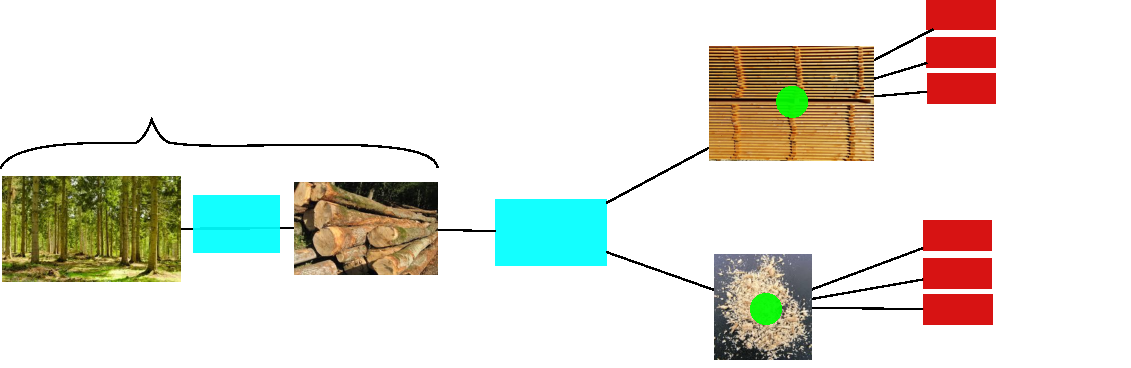
\includegraphics{/home/rudy/Documents/rudy/01_These/11_production/01_COMMUNICATION/figures/alloc_value_integrated_20160226.pdf_tex}
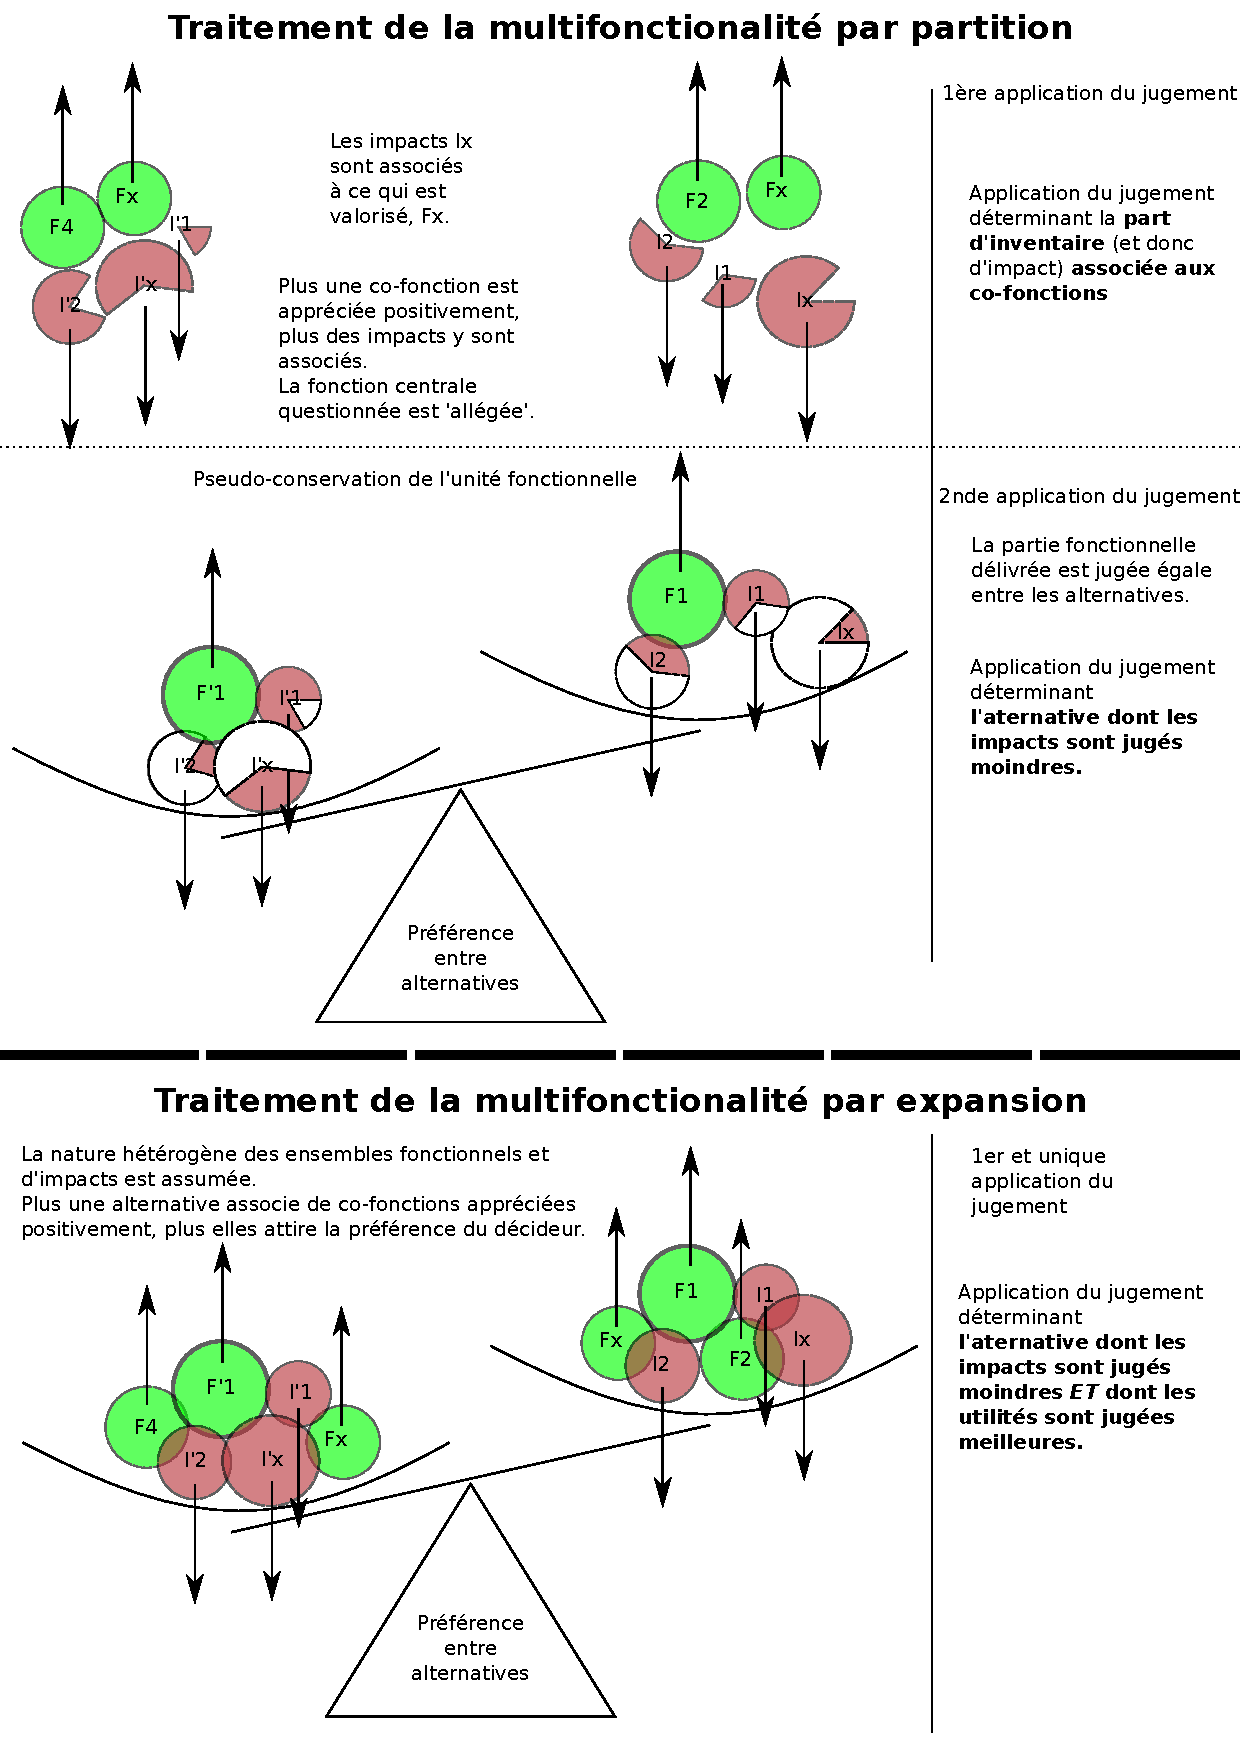
\includegraphics[width=0.9\textwidth]{/home/rudy/Documents/rudy/01_These/11_production/01_COMMUNICATION/figures/partition_expansion.pdf}
% à remettre dans le .pdf_tex après modif : /home/rudy/Documents/rudy/01_These/11_production/01_COMMUNICATION/figures/
\caption{Partition et Expansion, quelles différences ?}
\label{fig:partition_expansion}
\end{figure}

%\begin{tcolorbox}[
%%					colframe=red!50!white,
%					width=\textwidth,
%%                  enhanced,
%%                  frame hidden,
%%                  interior hidden,
%                  boxsep=2pt,
%                  left=2pt,
%                  right=2pt,
%                  top=2pt,
%                  ]
\figbox{
La figure~\ref{fig:partition_expansion} représente par la symbolique de la balance le processus comparatif et le traitement de la multifonctionnalité d'abord par partition puis par expansion.
\keybox{
Il n'y a pas de véritablement 'meilleure' alternative mais uniquement des alternatives \emph{préférées}.
La question est donc de savoir quelle alternative est réellement préférée par le décideur.}
Il faut donc une unicité du jugement employé.
Les modes de traitement de la multifonctionnalité, consistant avec le caractère multi-critère de l'ACV, restent donc la partition multi-critère et l'expansion.
Dans le premier mode de traitement, le jugement du décideur est appliqué d'abord pour isoler l'unité fonctionnelle à la base de l'étude.
Puis il est appliqué une seconde fois pour déterminer l'alternative préférée parmi celle délivrant cette même unité fonctionnelle.
Ce premier type de traitement se limite donc à la confrontation de systèmes répondant à (au moins) une même fonction.
Dans le second mode de traitement, c'est l'ensemble des fonctions et impacts de chaque alternative qui est confronté aux autres.
\textbf{Il n'y a plus unicité de la fonction.}
Le jugement n'est appliqué qu'une fois sur la globalité de la confrontation.
Il sera donc remarqué que l'ensemble des jugements sur les fonctionnalités et impacts doit être disponible de façon globale et consistante.
}
%\end{tcolorbox}

%\colorbox{yellow}{ application numérique, reprendre fichier test allocation.ods et test electre.r}

%\subsection{Application comparée}
%
%Soit le cas (a) de la table~\ref{tab:allocation_partition_cas_dissociables}.
%Posons le cadre d'application~: un décideur s'interroge sur le choix entre le produit 1c et 2a.
%Ajoutons maintenant une donnée d'inventaire liée à un impact, disons~: 6~kg CO2 au produit 1 et 1~kg CO2 au produit 2.
%
%Puisque le système de valeurs intervenant ne porte plus uniquement sur le traitement de la multifonctionnalité mais la préférence entre deux modifications d'états alternatives (impacts), étendons le système de valeur.
%
%Le jugement sur les aires de protection est le suivant~:
%\begin{table}
%  \begin{center}
%  \caption{Matrice de comparaison par paires, visant les aires de protection, remplie à titre d'exemple. CI 0.0013 ; CR 0.0023}
%  
%  \begin{tabular}{| c|c |c |c |c|}
%  \hline
% & Éco-système & Vie humaine & Ressource & Priorité \\ 
% \hline
%Éco-système & 1     & 2     & 7     & 0,62 \\ 
%Vie humaine &  1/2 & 1     &  3 & 0,29 \\ 
%Ressource &  1/7 & 1/3     & 1     & 0,09 \\ 
%  \hline
%  \end{tabular}
%  \end{center}
%  \label{tab:3_attributs_impacts}
%  \end{table}
%Si l'on considère une architecture des valeurs où les dimensions monétaire, énergétique et massique porte sur la distribution des ressources, alors la hiérarchie définie à la table \ref{tab:exemple 3 attributs}, est incluse sous celle des aires de protection dans l'espace des ressources.
%Ceci nous donne le coefficient 0.09 en facteur sur ces valeurs.
%
%%Poursuivons notre application avec la position d'un acteur à but lucratif, pour lequel, les alternatives ont donc pour fonction principale d'être rémunératrice (conformément au système de valeur exprimé pour l'allocation).
%%Notons la contradiction sur les aires de protection...
%
%\subsubsection{Traitement par partition}
%La produit 1c est caractérisé par~:
%La fourniture de 13 EUR, 32 kg (mat non précisée) et l'émission de 6~kg~CO2 (en co-fonction avec le produit 2c), attribué à 37.1\% à 1c (soit 2.226~kg~CO2).
%La produit 2a est caractérisé par~:
%La fourniture de 8 EUR, 7 kWh (niveau énergétique non précisée) et l'émission de 1~kg~CO2 (en co-fonction avec le produit 2c), attribué à 60.7\% à 2a (soit 0.607~kg~CO2).
%
%Posons le surclassement suivant (cf section mcdm~\ref{mcdm}).
%
%\colorbox{yellow}{proposer un exemple avec promethee et un avec electre}
%
%\colorbox{yellow}{ré-installer les outils numérique ? (galère à la main)}
%
%\colorbox{red}{pas fini}
%%π(a,b)=∑j=1kwjPj(a,b)
%$ \pi(a,b)=\sum j=1kwjPj(a,b) $
% \begin{table}
%   \begin{center}
%   \caption{Surclassement entre 1c et 2a}
%   
%   \begin{tabular}{|c |c |c|}
%   \hline
%  critère & surclassement & puissance \\ 
%  \hline
% Éco-système &      & 2     \\ 
% \hline
%% Ressource &  1/7 & 1/3     \\ 
% Eur &  1c P 2a & 1     \\
% kWh &  2a P 1c & 1     \\
% kg & 1c P 2a  & 1      \\  
%   \hline
%   \end{tabular}
%   \end{center}
%   \label{tab:ex_surclassement}
%   \end{table}
%\subsubsection{Traitement par expansion}

%\section{La dimension politique}

\newpage
\section{Conclusion sur la multifonctionnalité}
\label{sec:Conclusion sur la multifonctionnalité}
\keybox{
La multifonctionnalité en ACV était un problème non encore résolu.
Plus qu'une formulation ambiguë des questions d'allocation~\cite{weidema_has_2014},
les limitations de l'ISO~14040 résident dans l'absence d'un élément central~: \emph{l'intégration globale, consistante et explicite, du jugement moral des parties-prenantes}, pour la résolution de cette question.
}
%xxxxxxxxxxxxxxxxxxxxxxxxxxx

Les caractéristiques à prendre en compte sont autant physiques qu'humaines.
Englober à la fois les perspectives physiques et socio-économiques, c'est tenter une réconciliation entre valeur d'usage et valeur d'échange, dans la continuité de travaux de longue date d'économistes antiques comme modernes~\cite{harribey_richesse_2013}.
C'est refuser d'accepter la seule lecture de la valeur imposée par la classe dominante.
C'est unir les dimensions de la réalité plutôt que de déterminer, ou imposer, une séparation et une hiérarchie entre elles comme certains le proposent~\cite{pelletier_rationales_2014}
\footnote{
\blockcquote[traduction]{pelletier_rationales_2014}{
Nous concluons que la hiérarchie de multifonctionnalité de l'ISO~14044 devrait explicitement faire une distinction entre les applications de modélisation des données attributionnelles et conséquentielles.[\ldots]

Nous suggérons que la norme ISO 14044 devrait également rendre explicite sa rationalisation pour \emph{privilégier les approches fondées sur les sciences naturelles} pour résoudre les problèmes de multifonctionnalité et de \emph{différencier plus clairement les approches fondées sur les sciences naturelles et  sur les sciences sociales.}
%We conclude that the ISO 14044 multifunctionality hierarchy should explicitly differentiate between attributional and consequential data modeling applications.
%(...) We suggest that ISO 14044 should also make explicit its rationale for \emph{privileging
%natural science-based approaches} to solving multifunctionality problems and to \emph{more clearly differentiate between natural science and social science-based approaches}
.}
}.

Parmi les dimensions objectives, nous relevons également l'importance pour les grandeurs extrinsèques d'une documentation riches des flux des produits et de leurs caractéristiques.
Le traitement par destination nécessaire notamment à la résolution des multifonctionnalité pour les semi-produits implique une documentation plus ouverte des processus industriels.
La tendance à la protection des secrets industriels pourrait bien priver les sociétés humaines de décisions rationnelles.
L'alternative à une donnée primaire issue des sites effectifs serait une reconstitution depuis la documentation des processus connus et employés dans les entreprises ouvertes (fonction publique ou établissement fonctionnant sur la base de l'open-source).

%Cette thématique, débutée semble-t-il avec \textsc{Aristotle}, est plus récemment traitée par \textsc{Harribeys}~\cite{harribey_richesse_2013}.
La recherche d'un traitement holistique est le rappel du caractère multidimensionnelle de la réalité et de l'\emph{incommensurabilité} de ces dimensions.
C'est reconnaître la multiplicité et la complexité, pour \emph{ne pas imposer de jugement unique}.

%Encompass both physical and socio-economic perspectives~\cite{pelletier_rationales_2014} is trying a reconciliation between use and exchange values.
%Question of what matters or matters most, 

%%This matter, discussed by \textsc{Aristotle}, is more recently browsed by \textsc{Harribeys}~\cite{harribey_richesse_2013}.
%Summing up this we would say, money has no monopoly on richness. %\footnote{"Richness" is used here to avoid a misleading use of "value" monetary value.}.
De surcroît, il est difficilement envisageable que notre société évolue vers une alternative \emph{soutenable}, pour elle toute entière, dans un saut à un système de valeur entièrement nouveau.
Il est en tout cas certain qu'une évolution vers une soutenabilité forte ne pourra se faire sur la base des deux principes~:
%\begin{enumerate}
(1) Les praticiens acévistes ne doivent pas mélanger les clefs d'allocation.
(2) L'allocation économique est le cas général.
%\end{enumerate}
%Furthermore, we can hardly imagine our society evolve in a jump to an alternative set of governing values.
%For sure it cannot be achieved while keeping the two statements: 1) LCA practitionners should not mix allocation keys 2) Economic allocation is the general case.

Alors que nous réalisons la sélection des \emph{valeurs} déterminantes du système, n'oublions pas~:
%\begin{itemize}
(i) les applications de l'information produite,
(ii) qui prend la décision
et (iii) qui en supportera les conséquences.
%\end{itemize}
L'ACV est utilisée pour \emph{Le développement des Produit} dans une économie globalisée ; en \emph{Marketing} et les produits discutés peuvent couvrir la planète ; en \emph{Planification Stratégique} et à l'\emph{élaboration des réglementations publiques}~\cite{european_commission_ilcd_2010}.\\
\textit{Ainsi, par ces évaluations sont écrites les orientations de ce qui va être,\\
et les conséquences qui seront supportées par tous, ainsi que ceux à naître.\\}
%While eliciting values, shall we not forget applications of the produced informations.
%\emph{Who} is the \emph{decision maker} and \emph{who will support the consequences}.
%\cite[Framework for life cycle assessment (from ISO 14040:2006; modified)]{european_commission_ilcd_2010}.
%LCA is used for ``\emph{Product development and improvement}'' in a global economy.
%It is used in ``\emph{Marketing}'' and the discussed product can cover the globe.
%It is used for ``\emph{Strategic planning}'' and ``\emph{Public policy making}''.
%So orientations of what will be tomorrow are written there and \emph{the consequences will be borne by everyone even those yet to be born}.
Conséquemment allons un pas plus loin dans le sens de la déclaration de \textsc{Mathe}~\cite{mathe_integrating_2014}.
Intégrer les parties prenantes n'est pas uniquement \emph{intéressant}, c'est une \emph{nécessité}.
%Consequently we propose going a step further with respect to \textsc{Mathe}'s statement~\cite{mathe_integrating_2014}.
%Integrating stakeholders participation is not only \emph{of interest}, it is \emph{necessary}. % to avoid LCA's failure.
Il est donc apparu crucial de concevoir une méthodologie permettant une modification interactive et progressive du système de valeurs à la base de nos décisions. 
%So we devised a consistent method allowing for a progressive and interactive modification of the value balance.

%xxxxxxxxxxxxxxx


Nous avons exposé l'usage du modèle multicritère produit pour l'allocation et ses résultats sur des sorties (flux sortants) \emph{hétérogènes}.
Nous avons souligné l'importance de développer les priorités sur l'\emph{ensemble} des valeurs manipulées en ACV \emph{avec} les parties-prenantes.
%We exposed its use for allocation and its results on heterogeneous outputs and stressed out the need to develop priorities on \emph{all} values handled in LCA \emph{with} stakeholders. 
\keybox{
Comme des attributs incommensurables\footnote{Sans commune mesure.} sont en jeu, \emph{nous ne pouvons pas nous passer de l'expression d'opinions}.
La capacité de l'ACV à se développer en tant que science sera directement liée à notre capacité à dissocier observations, opinions et leur traitement conjoint.
Les façons dont nous organiserons la détermination des jugements de valeurs pour nos processus de décisions seront les miroirs de nos cultures.}
%As incommensurable attributes are at stake, \emph{we can not bypass the expression of opinions.} % if we are to include these attributes}.
%The capacity for LCA's field to develop as a science will be the direct result of our ability to dissociate observations,
%% and its data, the needed 
% opinions and the processing of both.
%The way we will organize this values elicitation in our decision process will be the mirror of our societies cultural portraits.

Il convient donc de modifier en conséquence la norme de l'ACV.
La modification est représentée au~\ref{sec:Un nouveau standard}.
L'étape de déclaration de valeurs, pour des raisons de consistance, devrait viser à la fois les attributs des flux pour le traitement de la multifonctionnalité et les impacts pour l'interprétation.
%Allocation in LCA is an issue.
%But more than ambiguous phrasing of multi-functionality treatment~\cite{weidema_has_2014}, %in my opinion
%ISO~14040
%%serie
%'s limitation lies in its lack of a central key element: \emph{explicit stakeholders value judgements integration}.
%The value declaration step should target both attributes for allocation and impacts for interpretation %.
%It should
Cette étape devrait être traitée avant même la définition du but de l'étude~\cite{patard_life_2015}.
%and
%it should be treated before defining the goal of the study~\cite{patard_life_2015}.
Elle serait une étape indépendante de l'ACV, bien que fournissant une part d'information cruciale à sa réalisation.
Réaliser ce 'découpage' permettrait un processus de revue effectif des ACV.
L'application effective du jugement du décideur pourrait être contrôlée.
Les bases de données contiendrait alors les descriptions des systèmes techniques, environnementaux et sociaux.
Il serait donc possible de fournir ce qui est requis par certains auteurs \blockcquote{majeau-bettez_unified_2014}{la dissociation de l'observation (inventaire) de la modélisation}.
%It is an independent step of LCA, even though providing necessary information for it.
%Doing so would allow effective reviewing process %.
%and
%%It would 
%enable LCA to effectively reflect the judgement of the decision maker(s).
% would be independent of the judgement.
%Databases would then be systems descriptions for social, environmental or technical information.
%It would then become possible to deliver what is required by some authors\blockcquote{majeau-bettez_unified_2014}{to dissociate the observation (inventory) from the modelling}.

Nous allons donc dans la partie suivante observer comment produire cette unicité du jugement. %chapter
\chapter{Jugements et Multi-dimensionnalité}
\label{chap:Jugements et Multi-dimensionnalité} %, indicateurs et interprétation} % lien de l'impact à la fonction entre inventaire et modélisation, déjà l'interprétation.
Au sein de la méthodologie et comme observé dans la revue critique de \citeauthor{reap_survey_2008}, un certain nombre de points sont des "décisions pivots".
Nous venons de faire la démonstration de la résolution de la problématique de la multifonctionnalité et nous affirmons qu'il en va de même sur l'ensemble des jugements dans la méthodologie.
Et puisqu'il s'agit d'observer l'ensemble des applications de jugements moraux au sein de la méthodologie pour corriger celle-ci, reprenons cette liste et traitons les, point par point, dans l'ordre méthodologique proposé en ISO et ILCD.
Sur cet ensemble, nous rechercherons les dimensions employées et leurs articulations entre les diverses questions.
À l'issue de ce déroulement, nous ferons la synthèse des dimensions et tenterons de proposer un ensemble cohérents de celles-ci sur lequel poser le jugement du décideur, l'\emph{interprétation finale}.

\section{Un ensemble de jugements}
%\colorbox{yellow}{avec ou sans le chapeau du chapitre ?}
%
%\colorbox{yellow}{intégrer Hafizan dans les applications (AHP sur les indicateurs)}

 \citeauthor{reap_survey_2008}, dans leur article, définissent les choix de l'exécutant comme décisions centrales (pivotal decisions, marqué d'un~"~a~" dans la table \ref{tab:PB non-resolus de l'ACV}).
 
!!!!!!!!!!!!!!!!!!!!!!!!!!!!!!!!!!!

 \colorbox{yellow}{check}
 
 reprendre table en fr pour reconstruire l'image
 
!!!!!!!!!!!!!!!!!!!!!!!!!!!!!!!!!!!
 
  \begin{figure}[h]
  %  \textwidth*0.5 : pas fonctionné
  %  figure à créer depuis le poster
    \centering
    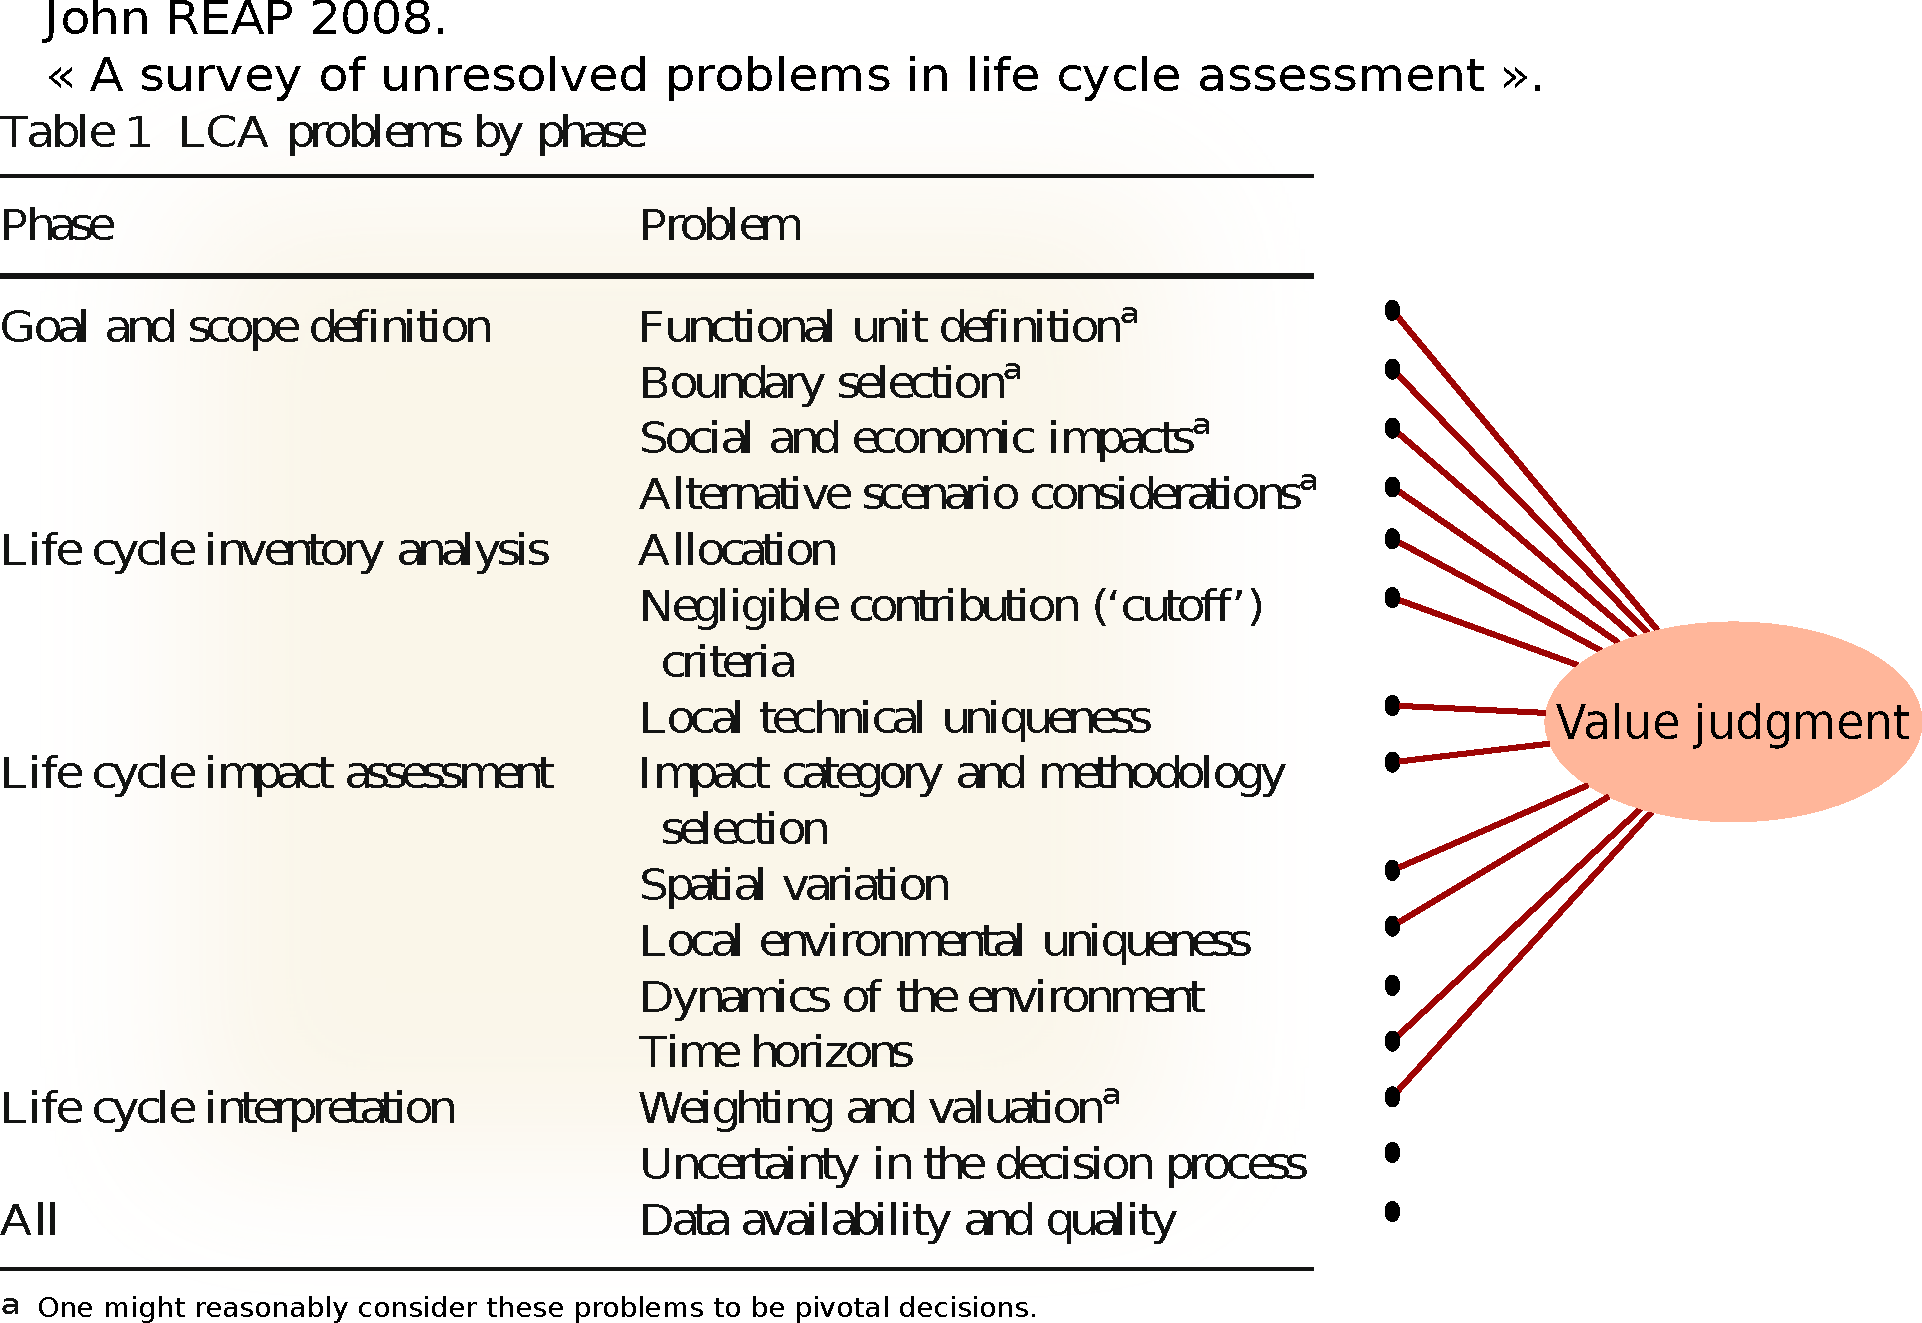
\includegraphics[width=\textwidth]{/home/rudy/Documents/rudy/01_These/11_production/01_COMMUNICATION/figures/value_quite_everywhere.pdf}
    \caption{Une multitude de jugements.}
    \label{fig:multitude_jugements}
  \end{figure}
Nous pouvons commenter le tableau~\ref{tab:PB non-resolus de l'ACV} en ajoutant que la sélection des méthodes et indicateurs d'impacts est également un choix du praticien.
Cette sélection peut s'apparenter à une pondération nulle des indicateurs existants mais qui n'ont pas été retenus dans l'étude.
De même les considérations qu'une différence temporelle, spatiale, technique, quantitative soit, ou non, négligeable ou non considérée est un jugement.
Comme nous venons de nous étendre sur la question de la multifonctionnalité, l'allocation relève tout autant de cette catégorisation.

Passons donc en revue chacune de ces questions.


%\subsection{How does the practitioner define the functional unit?}
\subsection{Définir l'unité fonctionnelle~?}

\exbox{
Un kilogramme de grain de blé pour produire de la farine n'est pas un kilogramme de grain de blé pour produire des pâtes (wheat grain, durum grain).
Nous tendons à réduire les entités aux attributs que nous connaissons à leur propos et plus encore à ceux que nous jugeons importants.
Nous oublions parfois que l'importance de la distinction entre des entités peut venir de la simple existence de la différence elle-même~\cite{corrado_new_2010}.
}

Pour dissocier ces produits similaires, il faut prendre en compte de plus nombreux attributs que la masse seule.
Ainsi, lorsque le praticien choisi l'unité fonctionnelle, il sélectionne relativement au produit observé ce qui selon \emph{lui} fait \emph{valeur}.
Donc, l'une des premières actions du praticien suivant les étapes de l'ISO ou de l'ILCD~\cite[]{european_commission_ilcd_2010}, ou du PEF~\cite{commission_europeenne_commission_2013}, est l'application d'un jugement de valeurs.
Il sélectionne les attributs et leurs combinaisons qui font sens relativement à sa propre perception de ceux-ci.
Pour prendre de la distance avec une perspective fonctionnaliste (nous rapprocher des systémistes), nous pouvons considérer que chaque flux apprécié comme fonctionnel est un flux portant des attributs que nous valorisons.
Nous pouvons donc dire que le système observé n'est pas un objet fonctionnel, mais simplement un système, avec des entrées et sorties en relation avec son environnement.
Ce faisant, nous reportons le jugement d'utilité, de fonctionnalité ou de valeur, au delà de la caractérisation objective.


%Example:
%
%One kilogram of flour grain to produce bread is not one kilogram of flour to produce pasta
%\footnote{We tend to reduce entities to the attributes we know about them and to those we consider ``important''.
%We some times neglect that some  entity we juge as a lesser one for its properties we judge at this time useful remain interesting and potentially important simply by its existence~\cite{corrado}}.
%To discriminate those similar products you have to take into account more numerous attributes than weight.
%\emph{So when the practitioner choose the functional unit, he's selecting what makes value to him.}
%So the first thing the practitioner do following ISO or ILCD\cite[]{european_commission_ilcd_2010} or PEF is making a value judgement.
%He selects the attributes and their combination that make sense according to his own perception of those attributes.
%To take distance with the functionalist perspective, we have to consider that the flow we consider functional are only flows with attribute we value.
%Then the system observed is not a \emph{functional } object, but rather an entity with input, output, in relations with its environment.
%And doing so we report the judgment of utility (or functionality), of value, outside of the characterization of the object (product or services).

%\subsection{How are selected boundaries?}
\subsection{Déterminer les frontières}
%\colorbox{yellow}{INSERT CRADLE|GATE|USE|GRAVE boundaries| si abs image libre, créer}

\textbf{Faut-il définir des frontières ou de définir des règles d'inclusion - exclusion~?}

Le périmètre est une conséquence directe de l'unité fonctionnelle.
Il s'agit de \textit{dé\textbf{finir}} (poser une fin) à ce qui contribue à la délivrance du flux de référence.
Cela concerne ce qui est appelé par certain praticien et chercheurs comme `premier plan'.
Ceci est repris dans l'ILCD.
\blockcquote[Figure 13, p., traduction]{europ}{
Représentation du système de premier plan et du système d'arrière-plan dans la perspective de la spécificité (voir encadré);
(À titre indicatif): Le système analysé a des limites (frontière en pointillés), la séparant du reste de la technosphère et de l'écosphère.
Le système peut être divisé en premier [et arrière] plan.
[Le premier plan est] le système des procédés qui sont spécifiques au système analysé, c'est-à-dire propres opérations et les fournisseurs fixes.
Les procédés dans le système d'arrière-plan ne sont pas spécifiques, mais acheté par l'intermédiaire d'un (théoriquement totalement homogène) marché.
Le système est la somme exacte de l'arrière-plan et des systèmes de premier plan.
Quantitativement flux non-pertinents peuvent être exclus, i.e. une coupure est pratiqué [cut-off] (flèches en pointillés).}
%Foreground system and background system in the specificity perspective (see box); (illustrative): The analysed system has boundaries (dashed border), separating it from the remainder of the technosphere and from the ecosphere. The system may be divided into the foreground system of processes that are specific to the analysed system i.e. own operations and fixed suppliers. The processes in the background system are not specific but purchased via a (theoretically fully homogenous) market. The system is the exact sum of the background and the foreground systems. Quantitatively irrelevant flows can be excluded, i.e. cut-off (dotted arrows).
%}
Cette contradiction méthodologique est le résultat des approches pré-informatique où il n'était pas envisageable de laisser numériquement converger un calcul puisqu'il était (et est toujours) réalisé par voie analytique et inverse de \textsc{Leontief}.

Dans les études de cas nous rencontrons différents types de frontières.
Des études sont définies `jusqu'à la~: porte, roue, tombe.
Il s'agit des expressions ``cradle to door'', ``cradle to wheel'', ``gradle to grave''.
\textbf{Elles renvoient à des évaluations ne tenant pas compte de la totalité du cycle de vie.}
Quelles sont les raisons légitimes pour ces divisions~?
Ne serait-ce pas une expression inadéquate de l'unité fonctionnelle et de sa présentation à une audience~?
Observe-t-on la production d'un matériau ou produit semi-fini, d'un carburant, ou d'usages~?
Si nous sommes confiants dans nos raisons pour approcher la problématique de l'évaluation environnementale avec l'angle holistique de la \emph{\textbf{globalité} du cycle de vie}, alors pourquoi ces divisions ?

Si les coupures de périmètre de cette nature sont courantes mais discutées, il est une coupure bien plus profonde.
Dans le jugement des ``flux non-pertinents'' qui ``peuvent être exclus'' se trouve une coupure toute particulière.
Il s'agit de la notre, celle envers l’être humain.
L'ACV ne tient pas compte des composants humains des rouages entrepreneuriaux.

%Is there a need to define boundaries or rather rules for inclusion?
%Is there a legitimate reason for those divisions, gate, wheel and so on?
%Or is it just a bad expression of functional units and their depictions toward audience?
%Do we look at the production of fuel or use of a fuel...?
%If we were confident in the need to address impact assessment for all life cycle due to report of the stage the impacts occurs, then why those divisions?
\exbox{
Lorsque nous cherchions les limites du cas d'étude de cette thèse, les opérateurs manipulant le produit ont été considérés.
Le produit est-il fonctionnel sans l'action de cette personne~?
Il s'agit ici d'une question totale.
Non-Oui, Oui, car sans lui pas de produit.
Exclure un composant essentiel du système productif serait loin d’être une coupure anodine et somme toute donc une erreur.
Si l'opérateur est un composant décisif du système observé, alors il est légitime de l'intégrer au périmètre du système.
Nous n'avons jamais observé d'étude ACV qui pourtant s'en préoccupe.

Il s'agit ici d'une entité hautement multifonctionnelle.
Faut-il l'inclure dans le système, lui \emph{et} le système qui l'a formé, éduqué, protégé, soigné, logé, nourri, diverti etc. ?
La personne est \emph{employée} sur une fraction de son temps, de vie, d'activité.
Une part du système lui permettant d'être fonctionnel dans son \emph{emploi} pourrait donc être allouée sur la base de cette fraction (temps d'emploi / temps éveillé).
\textbf{N'est-il pas incohérent d'observer l'ensemble du cycle de vie pour les entités matérielles et ne pas le faire parce qu'il s'agit d'êtres humains~?}
}
Cet exemple, peut-être jugé caricatural pour certains, aura le mérite d'exposer ouvertement l'étendue du système à observer  dans une approche holistique.
Nous avons choisi cet exemple à dessein.
Il souligne particulièrement les distinctions qui pourraient être faîtes entre des systèmes technico-sociaux ou \emph{une part non négligeable de ces fonctions est assurée hors marché}, par des mécanismes de socialisation, étatique ou non.
%When searching the limits of the case study I've been hired for, I considered the operators handling the product, focus of the study\footnote{What was I thinking, hum!}.
%Is the production functional without this person ?
%If the operator is a decisive component of the system I observed, then she/he is a legitimate part of it and the boundaries shall include the operator.
%Be damed this component is highly multi-functional\footnote{I was sure it was gonna trouble me! I should stop thinking. This delays the deliverable way too much!}!
%Should I include part of the system that feeds her/him, that educated-s him/her, that protects, houses, heals, entertains her/him ... ?

Ainsi, déclarer l'importance du set de fonctions observées (considérées en services ou produits), est un choix de déclaration de valeurs envers un but perçu.
Le périmètre est la seconde étape respectivement à l'ISO.
Une nouvelle fois il s'agit, comme pour l'unité fonctionnelle, de l'application d'un jugement de valeur.

%So stating the importance to the set of function(s) observed (considered as services or products), is a choice of declaring the value toward a perceived goal.
%It is the second thing done according to LCA's guidelines and standards.
%It's still the same matters discussed for functional definition.
%It is still the elicitation of values and preferences.

%\subsection{What is considered negligible?}
\subsection{Considérer comme négligeable}
Sous ce thème je considère diverses formes de coupures (hors questions de périmètre).
Les originalités, techniques, spatiales, temporelles, environnementales, au sens ou elles sont des coupures qualitatives, comme les coupures quantitatives, ne doivent pas être traitées isolément.


%Under this question I consider all Cut-offs.
%Are uniquenesses negligible, ``Local technical uniqueness'', ``Spatial variation'', ``Local environmental uniqueness''?
%In the sense they are cut-offs of qualitative nature when cut-off usually addresses quantification.
%It is the same issue to me and cannot be divided in my opinion.
\exbox{
Posons-nous dans l'ordre les questions suivantes~:
\begin{enumerate}[noitemsep,topsep=0pt,parsep=0pt,partopsep=0pt]
 \item Combien de temps de votre vie considéreriez vous comme une coupure acceptable (cut-off)~?
 \item Combien de centimes de votre salaire considéreriez vous comme 'jetables'~?
 \item Quelle quantité alimentaire avez-vous laissé dans votre assiette lors de votre dernier repas~?
 \item Aviez vous préparé ce plat, attendu dans une file pour l'obtenir, payé pour qu'il soit devant vous dans cette assiette~?
\end{enumerate}
Ressentez-vous poindre lors de la question (4) l'inconsistance des réponses spontanément formulées entre (3) et (1+2).
%How much time of you life would you consider to acceptably cut-off?
%How many cent of you wages would you consider disposable off?
%How much food did you left to garbage in the plate of your last meal even-though you cooked it, waited in a queue for it or bought it?
}

Commençons par interroger la coupure quantitative.
En mécanique, certains matériaux sont caractérisés par leur résistance élastique.
Mais tous les matériaux ne présentent pas de palier pour distinguer un domaine plastique.
Un seuil arbitraire est alors définit (en \% d'allongement).
Ceci est fait parce qu'il n'y a pas de signe de convergence apparent sur une valeur à la frontière des domaines plastique et élastique.
Lorsqu'une courbe converge, la grandeur qui retient notre attention est la limite vers laquelle elle tend.
Ainsi, plus qu'un critère arbitraire de coupure quantitatif, ne devrions nous pas proposer une valeur de convergence de l'inventaire~\barre{?}~!
 
%In mechanic, some material are characterized by elastic strength.
%But not all material (particularly ductile one) have a yield stress to identify plastic domain precisely.
%The yield strength is then defined by an arbitrary off-set.
%This is done because there is no sign of convergence on some value to depict the frontier between plastic and elastic domains.
%When considering a convergent curve, by expressing a model of this curve, the convergence limit can be calculated.
%So more than the cut-off of LCI, shouldn't we propose a converged value of LCI?

Traitons maintenant la question qualitative.
Tant que nous disposons d'une information spécifique, pourquoi n'en ferions nous pas usage~?
L'agrégation des informations spécifiques suivant diverses classifications n'en sera pas moins exploitable lorsque l'utilisateur ne sera pas en mesure de préciser sa spécificité.
L'influence d'une application de données agrégées sous des catégories plus ou moins grandes sera sur la forme des fonctions de préférence sur les outils de surclassement cf~\ref{sec:ADMC}.

%As long as we have specific information, accordingly with restrained variability, I don't see a reason for not using it.
%The generic data still hold its variability and uncertainty.
%Either generic or not, they characterize the same object and using dissimilarly specialized data only interact with the preference form to consider when opposing the distributions.

%\colorbox{yellow}{GRAPH boxplot réduite et large. Pourquoi pas l'article sur les éoliennes de l'école BLANC}.
Actuellement au sein de l'ILCD, comme discuté par Lynda \textsc{Aissani}\footnote{Lors d'une formation EcoSD.}, l'utilisation de données spécifiques (non-génériques) "doit être justifiée"~\cite[Provisions: 6.7]{european_commission_ilcd_2010}
~\footnote{\blockcquote[Provisions: 6.7]{european_commission_ilcd_2010}{
XI) OBLIGATOIRE - Lieu et heure \textbf{méthodes d'AICV non génériques}: L'\textbf{utilisation} potentielle de méthodes d'AICV qui ont été dérivées des originales, celles comportant les localisations génériques et temporalités génériques (c-à-dire qui ne soient pas génériques, mais par exemple, spatialement ou autrement plus différenciées ou modifiées) \textbf{doit être justifiée} relativement à l'objectif et la portée de l'étude.
%XI) SHALL - Location and time \textbf{non-generic LCIA methods}: The potential \textbf{use} of LCIA methods that have been derived from the original, location-generic and time-generic ones (i.e. being not generic but e.g. spatially or otherwise further differentiated or modified) \textbf{shall be justified} along the goal and scope of the study.
}}
, alors que l'utilisation de données génériques, même si moins appropriées, n'implique pas cette justification.
%Currently within ILCD, as exposed by Lynda XXXXXX during EcodSD training, the use of specific methods ``shall be justified''\cite[Provisions: 6.7]{ilcd} when using generic even-though not the most appropriate is accepted without this justification.
Juridiquement nous dirions que la \emph{charge de la preuve est inégalement répartie suivant les défendeurs}.
C'est une problématique récurrente en science et en argumentation de façon générale\footnote{À titre d'exemple~:
\blockcquote{deshpande_signification_2011}{
[\ldots] la charge de la preuve est inégalement répartie
entre les deux camps.
\textbf{Les tenants d’une rupture avec le statu quo doivent être beaucoup plus convaincants que ceux qui se satisfont
de la situation actuelle.}
}
}.
Lors de l'application d'une orthodoxie, une vérité populaire, la vigilance scientifique ou critique chute. % (retrouver l'article de socio XXX ref). %\footnote{application marketing et cinématographique, les rire et applaudissement dans une série "comique"}.
%In law I would say the burden of the proof is unequally establish according to the defendants.
%We find here a recurrent issue of many sciences.
%When using orthodoxies, popular beliefs scientific vigilance drops\footnote{It works with all kind of vigilance. Citizens are also regularly fed with already accepted messages. This is interestingly developed in \citeauthor{} ?? bourdieux ? retrouver la video d'USUL et la source.}.
Il ne s'agit pas ici de dire que les hétérodoxes ne devraient pas avoir à se justifier.
Nous disons simplement que les orthodoxes le devraient également.
%It is not that heterodox should not justify themselves.
%It is that orthodox should too.

Sur un point plus spécifique, nous souhaitons également mentionner la différenciation des comportements normaux, anormaux et accidentels des systèmes étudiés.
L'article de \citeauthor{plumblee_marlos_2014} sur l'intégration des risques et événements non-ordinaires de la vie d'un produit montre les coupures que nous faisons sur les scénarios de vie considérés~\cite{plumblee_marlos_2014}.
L'intégration des données `qualité' et fiabilité (temps moyen entre deux défauts MTBF, qualification des défectuosités\ldots) pourrait tout à fait compléter nos modèles de descriptions.
L'intégration des questions de coût (LCC) le nécessiterait d'ailleurs pour plus de cohérence avec les charges d'assurances.
Il y a donc encore des corrections méthodologiques à apporter à l'ACV décrite dans les référentiels sur ce point.
%\footnote{
\exbox{
\blockcquote[traduction]{european_commission_ilcd_2010}{
Dispositions: 6.7 Préparation de la base d'évaluation d'impacts III.e)
Ils sont liés exclusivement aux flux élémentaires
(à savoir les interventions entre la technosphère et l'écosphère)
pendant des conditions de fonctionnement normales et anormales,
mais \textbf{excluant les accidents, les déversements et autres.} [ISO!]
%Provisions: 6.7 Preparing the basis for the impact assessment III.e)
%They shall be related exclusively to elementary flows
%(i.e. interventions between the technosphere and the ecosphere)
%during normal and abnormal operating conditions,
%but \textbf{excluding accidents, spills, and the like.} [ISO!]
}
}
%On a specific point I'd like to stress out a particular point on a qualitative cut-off, that is normal and ab-normal behavior of the studied system.
%It is defined in

Maintenons notre analyse des occurrences des jugements de valeurs dans la méthodologie.
Là encore, la détermination du périmètre en use sous de multiples orientations.
%But to remain in our list of modeling choices, again cut-offs are the judgment of importance (value) of additional data.
%And rules about cut-offs are questions of preference forms, i.e. how we value the difference between sets of data.
Sur le caractère quantitatif nous retiendrons, lorsque cela est possible, la recherche de la quantité `convergée' plutôt qu'une troncature d'une quantité déjà partielle.
Sur le caractère \emph{quali}tatif, nous retiendrons qu'il faut exclure l'exclusion méthodologique.
Ceci implique de pouvoir former à loisir sur la base des \emph{quali}fications des catégorisations pour l'accessibilité cognitive des parties-prenantes.
%\subsection{How should we consider time?} 
\subsection{Considérer le temps}
\label{subsec:Considérer le temps}
Sont incluses sous cette interrogation, la ``considération de scénarios alternatifs''
\footnote{
Ici, il s'agit des projections futures sur le système modélisé~\cite{reap_survey_2008}.
Elles impliquent des projections statistiques actuelles, mais aussi une orientation de 'où la société devrait-elle aller~?', aux travers des actions modifiant le "cap actuel".
},
l'"Environnement dynamique" et l'"horizon temporel".
Ces thèmes sont de même nature et traitent de notre rapport au temps, future mais aussi passé.
\citeauthor{murray_transdisciplinary_2015} rapporte les éléments suivants.

\blockcquote[traduction]{murray_transdisciplinary_2015}{
Hertwich et al. (2000)~\cite{hertwich_theoretical_2000} considèrent l'effet des valeurs dans la caractérisation telle que sur le potentiel de réchauffement climatique et l'actualisation des impacts futurs.}
Plus particulièrement \citeauthor{hertwich_theoretical_2000} font la critique de l'interprétation commune de la
\blockcquote[traduction]{hertwich_theoretical_2000}{
%According to a common interpretation, the
norme internationale sur l'ACV qui exige que les méthodes d'évaluation utilisées dans les comparaisons publiées soient ``libre de valeur''.
%international standard on LCIA requires that the assessment methods used in published comparisons be “value free.”
}
\keybox{
Nous retrouvons pour le temps comme tout autre dimension l'inséparabilité de l'é\textbf{valuation} et des \textbf{valeurs}.
}

\blockcquote[traduction]{murray_transdisciplinary_2015}{
Hellweg et al. (2003) examinent des raisons économiques pour l'actualisation et concluent que l'actualisation basée sur les «préférences temporelles pures» ne doivent pas être appliquées dans l'ACV pour des raisons éthiques.
}
Ceci souligne l’inconsistance propre à la vision courte de l'individu isolé.
\keybox{
Nous pourrions \emph{vouloir ne pas juger} du futur ou du passer, que nous ne pourrions pas.
Même considérer l'égalité de traitement sur l'ensemble de l'horizon temporel serait en fait un jugement.
}

Dans l'analyse de \textsc{Hellweg},
\blockcquote[traduction]{murray_transdisciplinary_2015}{
le type d'éthique n'est pas spécifié, mais semble être lié à la notion d'équité entre les générations.
Néanmoins, il est reconnu que les décideurs utilisent souvent des taux d'actualisation sur la base de préférence pure (définie par Hellweg comme «impatience»).
Hellweg et al. (2003) notent également que toute application d'une «valeur actualisée» pour les flux physiques suppose la \textbf{monétisation} et une série d'autres conditions telles que la \textbf{compensation} des générations futures et une approche de l'incertitude.
Le type de décideur et de leurs objectifs affectera également le choix du taux d'actualisation
(caractérisée par le taux de réduction privé ou social).
%Hertwich et al. (2000) consider the effect of values in characterisation such as global warming potentials and the discounting of future impacts.
%Hellweg et al. (2003) review economic reasons for discounting and conclude that discounting based on ‘pure time preferences’ should not be applied in LCA for ethical reasons.
%The type of ethics is not specified but appears to be connected to the notion of inter-generational equity.
%Nonetheless, it is acknowledged that decision makers often use discount rates based on pure time preference (defined by Hellweg as ‘impatience’).
%Hellweg et al. (2003) also note that any application of a ‘time cost of money’ to physical flows assumes monetisation and a range of other conditions such as compensation of future generations and an approach to uncertainty.
%The type of decision maker and their goals will also affect the choice of discount rate
%(typified by the private or social discount rate).
}
\keybox{
Nous voyons donc une domination de la discipline par un mode de pensée économico-monétaire chevillé à la substituabilité (généralisation du caractère compensable des choses).
C'est à dire que la discipline reconnaît ici sont échec face à la multi-dimensionnalité.
}
%I consider ``Alternative scenario considerations'' \footnote{here scenario considerations are future projection of the modeled system~\cite{reap_survey_2008}.
%They imply statistical projections, current state but should also integrate a Where does society want to go.},  ``Dynamics of the environment'' and  ``Time horizons'' to be of same nature, being the importance granted to future.


Il y a des inconsistances dans l'emploi disjoint de jugements de valeurs à travers les diverses étapes de l'ACV et la question de l'horizon temporel en offre un particulier.
%There are inconsistencies when not considering the value system for all the LCA steps, and ``Time horizons'' give us a good example.
Nous allons considérer les recommandations ILCD sur les méthodes d'impacts.
%On this case we will consider the ILCD recommendations.
Les méthodes d'impacts considèrent généralement trois horizons temporels issus des archétypes développés pour ECO-98.
Il s'agit des horizons à 20, 100 et 500 ans.
La recommandation par défaut est de 100 ans pour l'ILCD (3.1.6 Recommended default method at midpoint level)~\cite{jrc_ilcd_2011}.
Le manuel indique aussi la nécessité d'une représentativité temporelle correcte~\cite[6.8.4 Time-related representativeness]{european_commission_ilcd_2010}
%Impact methods consider three time horizons, 20, 100 and 500 years methods~\cite{jrc_ilcd_2011}.
%The guidance indicate the need for time representativeness \cite[6.8.4 Time-related representativeness]{european_commission_ilcd_2010}
\blockcquote{european_commission_ilcd_2010}{I) OBLIGATION - Bonne représentativité temporelle~: L'inventaire dans son ensemble doit avoir une représentativité temporelle aussi bonne que requise, en accord avec le but de l'étude.}
%\blockcquote{european_commission_ilcd_2010}{I) SHALL - Good time-related representativeness: The overall inventory data shall have an as good as required time-related representativeness, according to the goal of the study (see the accuracy requirements identified in chapter 6.9.2)}

Puis dans la procédure d'allocation décrite pour les co-produits, la formule est développée sur la fraction recyclée sans dépendance à l'échelle temporelle.
\exbox{
%In the allocation procedure described for co-product, the formula developed consider recycled fraction and process without time dependence.
% The allocation of the ``two steps allocation procedure'' lies in three part\footnote{I'm not kidding. Its juste the detailed three parts of the second step.}
%   \begin{enumerate}
%    \item Determination of the total use.
%    \item Sum of inventories of total use.
%    \item Mean of the previous sum.
%   \end{enumerate}
%   
%   ~\\
%   The total use quantity:~U
%   \footnote{
%   This is the result of geometrical progression of recycling a fraction of initial product (p) by a recycling rate (r).\\  
%   $u_2$ is the material quantity used after two recycling. $u_2= p+p*r+p*r^2$~\\
%   With $1+r+r^2+...+r^{n} = \frac{1-r^{n+1}}{1-r}$~\\
%   proof~:
% 
% \[ \left.
%     \begin{array}{rlcll} 
% 	Sn= &1&+&r+r^2+...+r^{n}& \\
%       r*Sn= &&&r+r^2+...+r^{n}&+r^{n+1}\\
%     \hline
%     Sn-rSn= & 1 && & -r^{n+1}\\
%     \end{array} 
%   \right. \]
%   $Sn=\frac{1-r^{n+1}}{1-r}$.}
% u'
% p
% r
% total amount of uses after first and second recycling loop
% primary amount
% average recycling rate [0...1), incorporating both collection efficiencies and processing
% efficiencies
% U
%  total amount of use
% i
%  recycling loop number
% n
%  total number of recycling loops
% 
   \begin{itemize}
    \item U~: quantité d'utilisation totale.
    \item i~: la boucle de recyclage.
    \item n~: le nombre de boucles de recyclage.
    \item r~: le taux moyen de recyclage, incluant à la fois la collecte et la transformation.
    \item p~: la quantité initialement produite.
   \end{itemize}
%   ~\\
   \begin{equation}
   U = \sum_{i=1}^{n}p*r^i=p*\frac{1-r^{n+1}}{1-r}
   \end{equation}
%   ~\\
%   ~\\
   L'inventaire du cycle de vie (ICV) de la quantité d'utilisation totale~:~I
   \begin{itemize}
    \item I~: ICV total d'une unité de produit (matière, pièce, vecteur d'énergie). % confirmer le terme, source, vecteur
    \item P~: ICV de la production par unité de produit.
    \item R~: ICV de l'effort de réutilisation, recyclage, revalorisation par unité de produit.
   \end{itemize}

L'inventaire complet suit la formulation~:
%The complete inventory I, is formulated as:
  \begin{equation}
   I = p*(P+W+R*\frac{r-r^{n+1}}{1-r})
  \end{equation}
%   Suivant le développement ci-dessous~:~\\
%   \[U=p+p*r+p*r^2+ ... +p^n\]~\\
%   \[U=p*(1+r+r^2+...+r^n)\]~\\
%   \[U=p+ \overbrace{p*r*(1 +r+r^2+...+r^{n-1})}^\text{Fraction réutilisée, recyclée, revalorisée, {\bf produite}}\]~\\
%   Il est important ici de comprendre la quantité à l'issue de l'effort R comme la quantité produite et non pas la quantité traitée !
%   
%The total use of the extracted material is developed as:
%  \begin{equation}
%  U = \sum_{i=1}^{n}p*r^i=p*\frac{1-r^{n+1}}{1-r}
%  \end{equation}
   Inventaire moyen d'une unité de produit~:~e
%The mean inventory is developed as
  \begin{equation}
  e= \frac{I}{U}=\frac{p*(P+W+R*\frac{r-r^{n+1}}{1-r})}{p*\frac{1-r^{n+1}}{1-r}}
  \end{equation}
%   
L'ILCD donne ensuite le raisonnement aux limites tel que~:
%With the consideration of ``infinite number of loops''\cite[Two steps allocation procedure, eq. 12]{jrc_ilcd_2010} in ILCD's guidance the share of inventory for waste treatment and primary production in the resulting average LCI/kg is only of the non-recycled part.
%And ILCD's guidance gives reasoning to limits as:
  \begin{equation}
  e=(P+W)*(1-r)+R*r 
  \end{equation}

Ceci peut être décrit de la façon suivante~:
En moyenne sur la somme des utilisations, les efforts de production primaire et de traitement des déchets (ultimes) ne sont comptabilisés que pour la fraction qui ne sera pas recyclée.
La production primaire et le traitement du déchet final sont très dilués par le cumul d'utilisation du recyclage
   \footnote{
   Le manuel rappelle que ce raisonnement suppose une égalité technique entre le bien primaire et le secondaire (recyclé, réutilisé ...).
   L'écart éventuel d'une génération sur l'autre doit être corrigé par un facteur
   \cite[14.4.1.2. Annexe C : modélisation de la réutilisation, du recyclage et de la valorisation énergétique]{european_commission_ilcd_2010}.
   Traduit de la version anglaise~:
   \blockcquote{european_commission_ilcd_2010}{Ce facteur de correction devrait être le ratio de prix de marché du produit secondaire sur primaire.}
   }
\keybox{
   Ce guide suit donc une logique de substituabilité marchande monétaire dont il ne semble capable de se défaire.
   }
   
   REPRENDRE LA TRADUCTION ou citation de la section ilcd et des equations correspondantes.
}
Pour ceux faisant l'effort d'appliquer la formule développée sans un nombre \emph{infini} de boucles, la \acrlong{MFA} nous montrera que certains secteurs peuvent 'stocker' la matière sur une durée importante (construction en tête sur plusieurs dizaines d'année)~\cite{davis_time-dependent_2007}\footnote{\citetitle{davis_time-dependent_2007}}.
Ce stockage souligne le délai temporel aux flux suivants (élémentaires comme produits).

And for those making the efforts of using the developed formula without this infinite number of loops [formula 11], MFA analysis shows us that may steel consuming sector is building and the good produced have long lifetime.

Accorder une part d'inventaire pour la fraction de matière qui sera potentiellement ré-employée dans une ou plusieurs centaines d'années et ne pas prendre en compte que l'activité extractrice a déjà eu lieu, ou est en cours, semble être un manque important de représentativité temporelle.
Granting a share of the inventory to a fraction of the material re-used in one hundred year from now and not take into account that extracting it was putting the burden on the environment \emph{now} is a serious lack of time representativeness to me.

De plus, il ne peut être déterminé aujourd'hui la quantité de ce qui sera recyclé aux taux et techniques actuelles ou à des taux spéculatifs ultérieurs.
Les suppositions et hypothèses des projections dépendent des jugements et des orientations que l'on souhaite pour le futur.
How much of what will be recycled can really be addressed by current rates of recycling, consumption and emission?
Quelles est alors la part effectivement recyclée dans l'horizon temporel sélectionné~?
What share is indeed recycled within the time horizon selected?
Ceci nécessite l'intégration des données de durée des procédés dans les descriptions de procédés et systèmes.
La dimension temporelle n'est-elle de toute façon pas nécessaire au traitement de la question des concentrations des substances émises~\barre{?}~!
According to the time horizons selection shouldn't we integrate lifetimes of products and lead-time production of processes?
Isn't the time dimension necessary anyway to address concentrations issues of all the substances handled?

Ici encore, sur plusieurs points nous avons vu l'importance de la considération du temps, de façon consistante, pour nous et les générations futures.
Here on several points, is considered value and relevance of time, ours and that of future generations, humans or else.
By not singling out the value system at play, the current methodology is inconsistent.

La perspective temporelle porte aussi une signification spécifique à un outil tel que l'ACV.
La modélisation du système vise aussi la localisation temporelle des choses changées suivant les alternatives.
Devrions nous considérer les alternatives pour les dommages passés ou futures~?
Si nous accordons toute l'importance au futur, rejetant de considérer un passé sans levier d'action actuel, allons nous générer une rétroaction permettant à une situation passée de se reproduire.
Sur quelle durée considérer l'influence de cette rétroaction, quand y-a-t-il prescription~?
Il faut donc déterminer un horizon temporel amont et un horizon temporel aval.
Concernant l'amont, il s'agit (au moins pour partie) de données objectives sur l’observation des rétroactions d'une production non-écoulée.
Time perspective also bears a specific topic for a decision tool such as LCA.
Modelling a system is also defining when (on top of where) things are changed.
Should I reconsider a choice of alternative for paste damage or incoming and future ones?
I chose to grant weight to future impacts considering that what matter is changing future emission, not those already made that I cannot change.
But granting positive feedback by consuming products responsible for these emission trigger their renewal.
So how long is this delay of past emission triggering negative feedback?
When start the environmental prescription to engage an alternative future?

% %!!! Keybox pb

\keybox{
Une part de cette dimension doit donc être traitée à la fois dans le domaine objectif et dans le subjectif.
\begin{itemize}
\item Le décideur considère comme important une plage temporel.
\item Un espace temporel objectif affecte l'espace subjectivement important.
\end{itemize}
Sans les lumières des sciences, point de rationalité consistante pour les jugements sur cette dimension.
}
%
%%\subsection{How should we value thing?}
%\subsection{Valoriser et apprécier les choses}
%La valorisation et l'appréciation englobent diverses interrogations.
%Nous regroupons ici les questions de "Pondération et évaluation", "Allocation" et "Sélection d'impacts".
%%Stated as ``Weighting and valuation'', ``Allocation'' and ``Impacts SelectionS''.
%Nous considérons la "Sélection des impacts sociaux et économiques " et la "Sélection des catégories et méthodes d'impacts " comme relevant du même thème, de la détermination des indicateurs observés, de la recherche de 'ce qui fait valeur'.
%%I consider ``Social and economic impacts selection'' as well as ``Impact category and methodology selection'' to be of the same nature of defining attributes of interest and the way to grant them value.
%
%Comme illustré pour l'unité fonctionnelle, le périmètre, l'appréciation des variations spatiales et temporelles, le problème est un tout portant sur l'attribution de la valeur au sein du système modélisé pour le décideur.
%Ceci peut être considéré comme le défaut centrale de l'\gls{ACV} dans sa méthodologie actuelle.
%
%%I kept this one to be the last but not the least.
%%As specifically illustrated for functional unit, boundaries or appreciation of time and spatial dimensions, the whole problem is to give value to attributes of the modeled system.
%%It can be considered the central lack within LCA's methodology to be corrected.
%
%Comme nous l'avions souligné pour la question du temps,
%les normes et manuels indiquent par exemple qu'il ne faut pas pondérer pour des assertions comparatives.
%Nous soulignons l'incohérence de l'ISO comme de l'ILCD par l'extrait suivant. 
%%\footnote{
%\exbox{
%\blockcquote[traduction]{european_commission_ilcd_2010}{
%5.2.5 Les comparaisons destinés à être divulgués au public
%(Fait référence à l'aspect de la norme ISO 14044: 2006 chapitre 4.2.2)
%[\ldots]
%Notez que, également selon la norme ISO 14044: 2006, une étude d'ICV seule ne doit pas être utilisée pour les assertions comparatives destinées à être divulguée au public, à savoir une évaluation de l'impact du cycle de vie et de \emph{l'évaluation} / interprétation \emph{doit être effectuée également}.
%}
%[\ldots]
%\blockcquote[traduction de la Dispositions: 6.7 Préparation de la base de l'évaluation de l'impact]{european_commission_ilcd_2010}{
%Normalisation et pondération: [\ldots]
%Notez que si l'étude comprend une assertion comparative devant être divulguée au public, \emph{la \textbf{pondération} quantitative des résultats des indicateurs publiés est \textbf{interdite}.
%}
%5.2.5 Comparisons intended to be disclosed to the public
%(Refers to aspect of ISO 14044:2006 chapter 4.2.2)
%
%Note that, also according to ISO 14044:2006, an LCI study alone shall not be used for comparative assertions intended to be disclosed to the public, i.e. a life cycle impact assessment and evaluation / \emph{interpretation shall be performed} as well.
%[\ldots]
%
%Provisions: 6.7 Preparing the basis for the impact assessment
%Normalisation and weighting:
%[\ldots]
%
%Note that if the study includes a comparative assertion to be disclosed to the public, \emph{quantitative weighting of the published indicator results is not permitted}.
%}
%}
%}.
Certains auteurs ont déjà souligné ceci

%~\cite{rowley_aggregating_2012,finnveden_critical_1999,hertwich_theoretical_2000}.
\citeauthor{rowley_aggregating_2012} supportant

!!? finnveden encore pb

%\citeauthor{finnveden_critical_1999}~\cite{finnveden_critical_1999} posent la déclaration suivante.
\blockcquote{rowley_aggregating_2012}{
Cependant, éviter la pondération exige du décideur d'appliquer une évaluation implicite, non-transparente, tel que d'attribuer à chaque critère une égale importance.
%However, avoiding weighting requires the decision maker to apply an implicit, non-transparent valuation such as to assign each criterion equal importance.
}
Or `attribuer à chaque critère une égale importance', c'est équi-\textbf{pondérer}.
Il n'est donc \textbf{pas question} en réalité \textbf{d'éviter quoi que ce soit}.
\keybox{
\textbf{Interdire la pondération est tout bonnement \emph{impossible}~!}
}

%Guidance and standard claim we should not weight for comparative assertion\cite[seek section]{jrc_ilcd_2011}. Authors enlist to the rule and confirm !!! HERE USE MORE EXEMPLES !!! 
%But there are also voices that rightfully stress out that it is impossible, not to weight.
%\blockcquote{rowley_aggregating_2012}{However, avoiding weighting requires the decision maker to apply an implicit, non-transparent valuation such as to assign each criterion equal importance.} 
%ROWLEY supporting \citeauthor{finnveden_critical_1999} ~\cite{finnveden_critical_1999}.

Concernant la section des impacts 'sociaux', nous avons vu section~\ref{sec:ACV social} leur diversité.
%Impact selection in S-LCA.
%\colorbox{yellow}{? bilbio ou ici, -> ref biblio et renvoi vref}
%
%La gamme offerte par la SHDB montre les catégories suivantes~\cite[slide:]{norris_tutorial_2013}:~:
%The range offered by SHDB shows the following categories\cite[slide:]{norris_tutorial_2013}:
%\begin{figure}[htbp]
%%  \textwidth*0.5 : pas fonctionné
%%  figure à créer depuis le poster
%  \centering
%  \includegraphics[width=0.5\textwidth]{/home/rudy/Documents/rudy/01_These/11_production/01_COMMUNICATION/figures_extraites/shdb_structure.pdf}
%  \caption{See the distribution of rights in: Labor rights, Human Rights, Governance categories. See the distribution of wealth in all categories.}
%  \label{fig:shdb_structure}
%\end{figure}
Nous pouvons recatégoriser ceux-ci en distribution, des ressources, des risques et des droits.
%I personally consider the resources, work, risks and rights and their distribution.
%\colorbox{yellow}{(reducible to resources and rights ?)}
De façon apparente, les thèmes des indicateurs dits sociaux ``Infrastructures Communautaires'', les services~: ``écoles, installations sanitaires, hôpitaux, infrastructure pour l'eau potable'' éclairent notre problématique.
Les valeurs discutées en évaluation d'impacts, accès à la santé, aux ressources, à un environnement stable \ldots services et biens en supports à la matérialisation de l'accès à ces aires de protection sont les mêmes que les valeurs discutées en allocation, en définition des unités fonctionnelles, des frontières, des coupures\ldots de tous les jugements de la méthodologie.
%Appearing clearly in social theme ``Community Infrastructure'', the services: ``school, sanitation, hospitals, drinking water'' enlighten a side of our issue.
%\emph{The values discussed in impact assessment} (access to health, resources, stable environment, services ... and the goods that support the materialization of these access) \emph{are the same than the values discussed in allocation, function definition, boundaries, cut-offs}.

C'est le cheminement présenté figure~\ref{fig:LCA_and_Values}, synthétisé figure~\ref{fig:LCA_and_Values2}.

%\begin{landscape}
\begin{figure}
%  \textwidth*0.5 : pas fonctionné
%  figure à créer depuis le poster
  \centering
  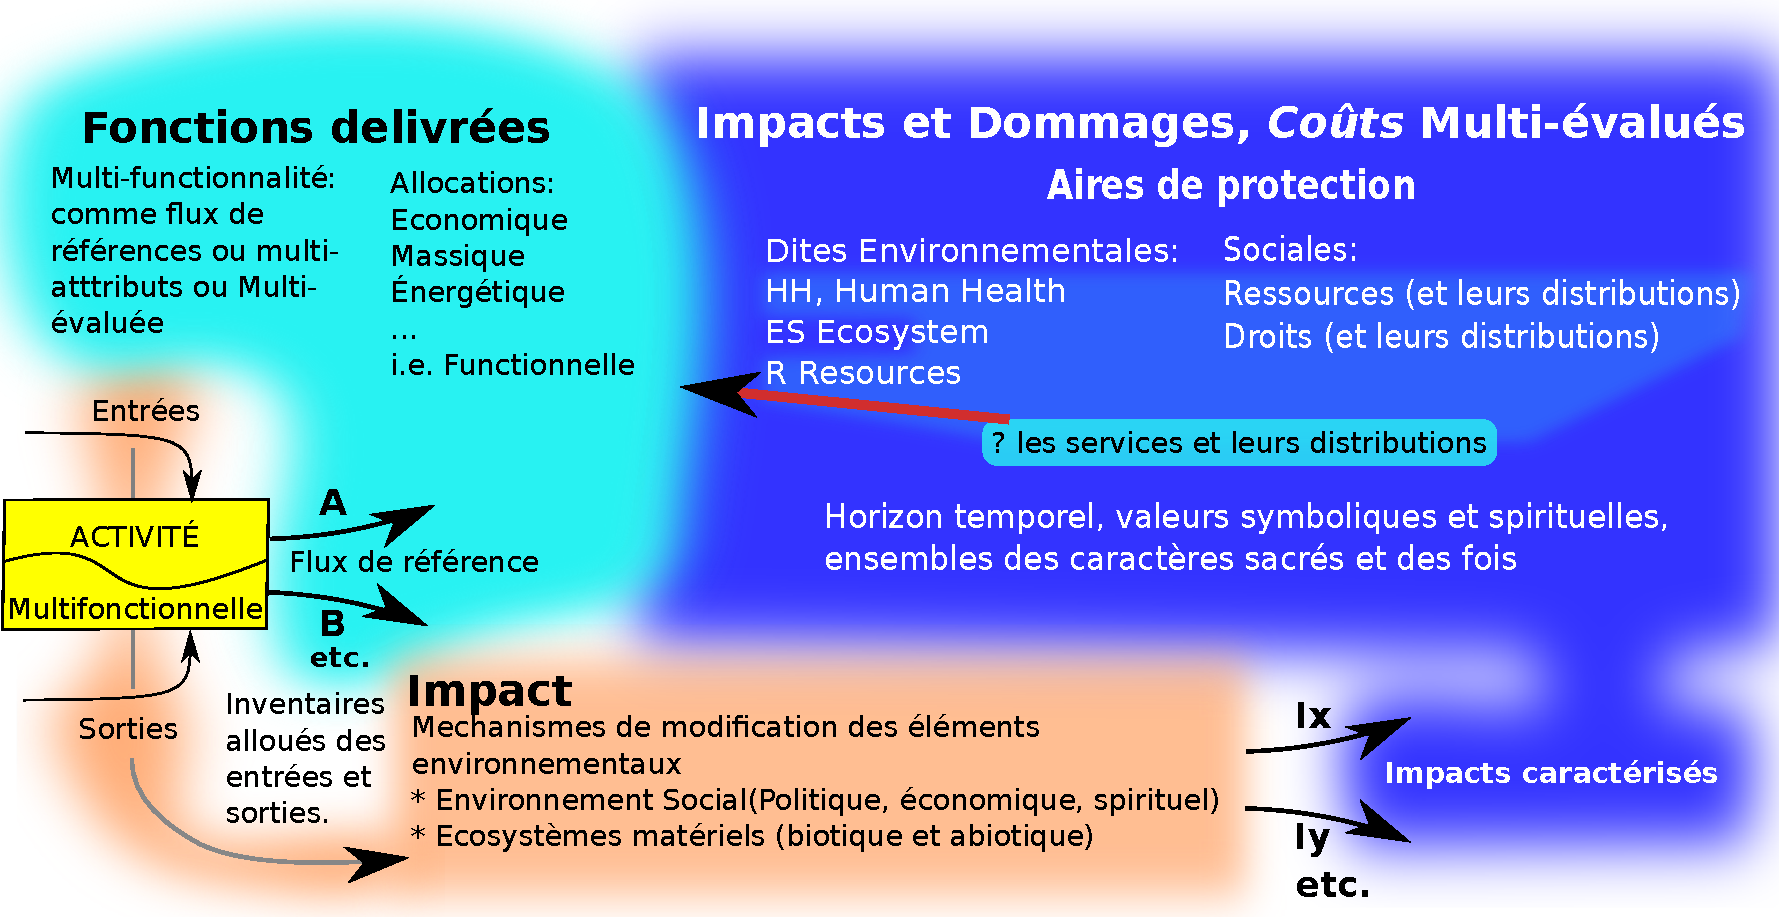
\includegraphics[width=1\textwidth]{/home/rudy/Documents/rudy/01_These/11_production/01_COMMUNICATION/figures/LCA_and_Values_FR.pdf}
%  \caption{We can see here that bringing S-LCA and LCA enabled us to link the domain of access to services to the services delivered (trough functions) to functional unit. And as a whole, the LCA balances values granted to attributes on the range of flows.}
\caption{Unicité des valeurs à l'inventaire et aux impacts.}
  \label{fig:LCA_and_Values}
\end{figure}
%\end{landscape}

\figbox{
Sur la figure~\ref{fig:LCA_and_Values}, nous partons du procédé (jaune), avec l'allocation entre les produits A et B.
Chaque produit, avec sa part d'inventaire et suivant les 'chemins d'impacts', endommagera des entités appréciées (jugé positivement utile), bien qu'apportant sa part fonctionnelle (jugée utile).
Il y a unicité des domaines des impacts et des services.
Ceci est particulièrement identifié sur les indicateurs sociaux et souligné par la flèche rouge relocalisant les services et leur distribution vers les fonctions délivrées.}

%\begin{landscape}
\begin{figure}
%  \textwidth*0.5 : pas fonctionné
%  figure à créer depuis le poster
  \centering
  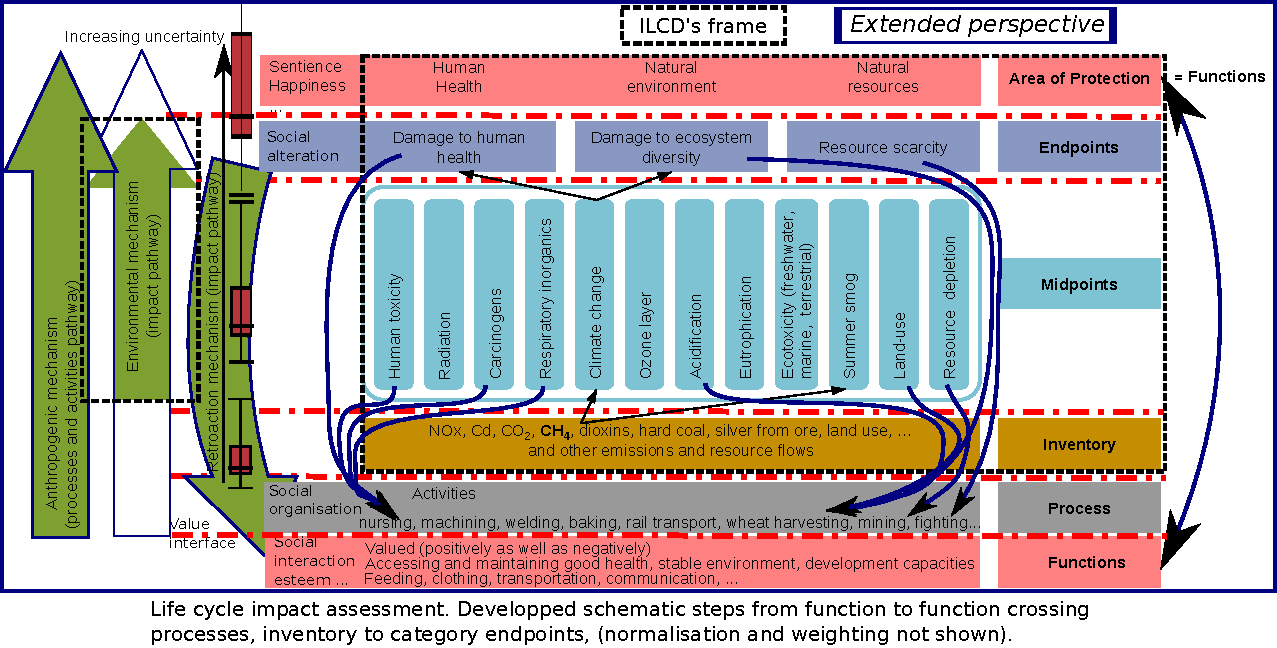
\includegraphics[width=1\textwidth]{/home/rudy/Documents/rudy/01_These/11_production/01_COMMUNICATION/figures/ILCD_LCA_LCIAM_extended_principles.pdf}
%  \caption{We can see here that bringing S-LCA and LCA enabled us to link the domain of access to services to the services delivered (trough functions) to functional unit. And as a whole, the LCA balances values granted to attributes on the range of flows.}
\caption{Représentation alternatives et synthétique de l'unicité des valeurs à l'inventaire et aux impacts.}
  \label{fig:LCA_and_Values2}
\end{figure}
%\end{landscape}

\figbox{
Sur la figure~\ref{fig:LCA_and_Values2}, le cadre de travail classiquement représenté (cadre pointillé) de l'inventaire aux indicateurs endpoint et étendu.
Il faut en fait partir des \emph{fonctions} délivrées par des procédés, des mécanismes, des \textbf{utilités recherchées} \emph{à produire}.
Les flux induits pas ces procédés (l'inventaire) généreront des impacts et des dommages (mid- puis end-point).
Ces dommages sont des dégradations des aires de protection.
Nous avons atteint les \textbf{utilités recherchées} \emph{à maintenir et protéger}.}
%The same issue in defining function, the domain and boundaries to include to complete this function, the allocation and valuation of impacts are the same problem of evaluating multi-valued object.

Il n'y a en fait que l'évaluation d'états différents (social wellfare).
Traiter l'ensemble de la démarche sous l'angle de l'évaluation multidimensionnelle semble en fait rejoindre les travaux de longue date des économistes~\cite{arrow_determination_1952}.
Plus particulièrement, l'angle de traitement de la multifonctionnalité par expansion (sans substitution ni mise à l'échelle) est assez proche de la confrontation de 'panier de biens multiples et hétérogènes' de \citeauthor{arrow_determination_1952} en \citeyear{arrow_determination_1952} avec \citetitle{arrow_determination_1952}.
Nous avons déjà donné une représentation de ceci dans la seconde partie de la figure~\ref{fig:partition_expansion}.

\section{Indicateurs \ldots d'autres méthodes ?}
Dans l'état de l'art, nous avons sommairement survolé la question des méthodes.
Nous ne sommes toutefois pas descendu jusqu'aux mécanismes de constitution des indicateurs.
Nous allons discuter ici le principe de description des mécanismes environnementaux et les indications associés.

En effet, les méthodes d'impacts produisent une indication numérique des impacts ou dommages potentiels sur la base des 'intrants' dans les 'mécanismes environnementaux'.
Poussons la description de l'environnement sur la même direction que les procédés de transformation de la matière.
Nos procédés techniques sont appliqués pour \emph{ajouter} une \emph{valeur}\footnote{Au sens richesse.} à une matière d’œuvre.
Nous jugeons comme dommage une modification d'une aire de protection lui ayant \emph{ôté} une part de \emph{valeur}\footnote{IDEM préc.}.
En fait, nous pourrions modéliser les méthodes d'impacts comme les mécanismes environnementaux dont elles ne seraient que des descriptions.

Une partie \emph{descriptive} n'inclue pas de \emph{jugement}.
Il s'agit donc de poser une description sur laquelle un jugement puisse être appliqué.
Il serait également judicieux de reprendre tout ou partie du langage des experts des domaines concernés.
Prenons des éléments de méthodes d'impacts et traitons les en cas d'exemples.

\subsection{Le cas du vivant}

Deux aires de protection des trois généralement admise porte sur le vivant (santé humaine et vie de l'écosystème)
Partons donc de l'observation des indicateurs sur le vivant.
Les méthodes doivent documenter les modifications que peuvent subir des éléments de l'environnement auxquels nous associons de la valeur sans anticiper cette appréciation ou dépréciation.

Prenons le cas de l'eutrophisation.
La documentation de la méthode ReCiPe 2008~\cite{goedkoop_recipe_2013}, indique concernant l'eutrophisation l'emploi d'autres modélisations (CARMEN :  CAuse effect Relation Model to support Environmental Negotiations, EUTREND).
La source citée mentionne malheureusement un manuscrit non publié~\footnote{Beusen A (2005). User manual of CARMEN1. National Institute of Public Health and Environmental Protection (RIVM), Bilthoven (\textbf{Manuscript, not published})}.
La figure 6.2 du rapport précité, documente la caractérisation en réduction du nombre d'espèces présentes (PDF potentially disappeared fraction).
Le rapport en mentionne un second de 2005 de la STOWA (Stichting Toegepast Onderzoek Waterbeheer, Fondation pour la recherche appliquée sur l'eau), absent dans leurs références.
Sans doute fait-il partie des publications accessibles de la STOWA \ldots \footnote{\href{http://www.stowa.nl/publicaties/publicaties/}{Lien vers les publications de la STOWA.}}

Pour autant, bien que maigre, la documentation a le mérite de faire partie des plus riches qui soient \emph{accessibles}\footnote{À comparer aux autres documentation de méthodes.} et nous permet d'identifier des sources des méthodes d'impacts.
Ainsi nous comprenons qu'une cartographie des concentrations des éléments C,H,O,N,P, ainsi que la documentation des métabolismes de la faune et de la flore, ainsi que de son recensement sur les territoires, permettrait de mettre en œuvre de façon continue la caractérisation de l'environnement.
Nous nous apercevons que la description `objective' est réalisé un pas plus tôt avant l'entrée dans le domaine actuel de l'ACV.
Il faut reculer cette frontière.
Une évaluation holistique opérationnelle doit opérer directement sur le champ objectif.

Puisque nous traitons ici dans ce chapitre des questions de dimensions, soulignons la suivante.
Au delà de la question spatiale, la dimension temporelle est également en jeu ici.
Nous avons traiter de cette dimension au~\ref{subsec:Considérer le temps}.
Le temps intervient dans les questions de toxicologie, tant envers l'homme que tout autre espèce vivante, mais aussi sur l'abiotique.
Les travaux récents sur l'acidification illustrent ce point~\cite{van_zelm_time_2007}.
Chaque indicateur, chaque dimension d'impact et sous l'influence de la dimension temporelle avec des écarts importants dans la caractérisation.
%\footnote{
\blockcquote[traduction]{van_zelm_time_2007}{
Puisque l'emplacement des émissions et des zones forestières sont connus et utilisés comme entrées dans les modèles de 'devenir' (fate of emission), \emph{il serait, en principe, possible de calculer des facteurs de caractérisation régionaux spécifiques pour l'acidification}.
À cet effet, les matrices source-récepteur spécifiques de la substance à un niveau des pays pour les modèles de transport atmosphérique de EUTREND doivent être développés et combinés avec le modèle SMART2.
%Since the location of emissions and forest areas are known and used as input in the fate models, \emph{it would, in principle, be possible to calculate region-specific characterization factors for acidification}. For this purpose, substance-specific source-receptor matrices on a country level for the atmospheric transport model EUTREND need to be developed and combined with the SMART2 model.
}
\keybox{
Toutefois, ce que nous retenons de ce type de travaux n'est pas uniquement la possibilité de calculer des facteurs régionaux spécifiques.
%}.
\textbf{Ce que nous retenons surtout, c'est la possibilité d'observer directement les modèles qui apparaissent dans ces publications (CARMEN, EUTREND, SMART2)}.
Tous ces travaux inaccessibles ou non publiés sont à la base des éléments objectifs pour la rationalisation des décisions.
Et parce qu'ils sont fondamentaux dans la constitution des indicateurs pour la décision, ils doivent être librement accessibles, vérifiables, reproductibles et exploitables.
}

Les travaux de \citeauthor{schmidt_development_2008} indiquent également une relation entre le territoire et sa caractérisation (convergence variable suivant la surface selon les zones caractérisées).
Dans ces travaux, l'horizon temporel choisi peut aussi affecter la prise en compte (ou non) de régénération future (ex : étalement du délai de `re naturalisation' "Renaturalisation time" de l'année à plusieurs milliers d'années)~\cite{schmidt_development_2008}.
Ainsi les inconsistances temporelles ont une forte influence sur le résultat par l'écart observé sur les facteurs d'impacts.

Pourrions-nous \emph{ne pas fixer} un découpage temporel pré-établi (pourquoi pas des horizons temporels à 150, 200, 250 ans)~\barre{?}~!
Laissons les décideurs définir le point de la courbe qui fera valeur pour eux.
Voyons ce point avec la toxicité et l'éco-toxicité et prenons la question sous le cas de l'indicateur \gls{DALY}, développé par \citeauthor{murray_quantifying_1994} dès \citeyear{murray_quantifying_1994}\footnote{\citetitle{murray_quantifying_1994} fut suivi d'autres publications d'explication et de justification~\cite{murray_disability-adjusted_2012,murray_global_1997,murray_evidence-based_1996,murray_quantifying_1994,murray_understanding_1997}. La volonté affichée est la \textbf{quantification objective}, basée sur des \emph{preuves} \citetitle{murray_evidence-based_1996}.}.

Reprenons l'article initial de \citeauthor{murray_quantifying_1994} et détaillons la présentation faite de l'indicateur point par point.
\blockcquote[traduction]{murray_understanding_1997}{
L'unité de mesure en années de vie ajustées sur l'incapacité (disability adjusted life years DALY)
[\dots]
% Utilisé ces dernières années pour quantifier le fardeau des maladies, des blessures et des facteurs de risque sur les populations humaines,
est fondée sur des principes économiques et éthiques convaincants et peut orienter les politiques vers la prestation de soins de santé la plus économiquement-efficace et équitable.
DALY suit un principe d'équité qui traite de manière égale ('like as like') l'ensemble des informations comprenant les conditions de santé des individus, différenciés uniquement par l'âge et le sexe.
Les \emph{poids} particuliers des états de santé utilisés pour tenir compte des résultats des pathologies non létales \emph{sont tirés de l'application de diverses formes de compromis personnels.}
%The measurement unit disability-adjusted life years (DALYs),
%[\ldots]
%%used in recent years to quantify the burden of diseases, injuries and risk factors on human populations,
%is grounded on cogent economic and ethical principles and can guide policies toward delivering more cost-effective and equitable health care.
%DALYs follow from a fairness principle that treats 'like as like' within an information set comprising the health conditions of individuals,
%differentiated solely by age and sex.
%The particular health state weights used to account for non-fatal health outcomes are derived through the application of various forms of the person trade-off.
}
%cogent = convaincant
%\begin{equation}
%\Delta _ {i j}^t  = \int_{a_i^t}^{a_i^t + L(a_i)} KD_jC_{xe}^{-\beta x}e^{-r(x-a_i^t)}dx
%\end{equation}

Nous observons que la seule dimension (et mesure associée) \emph{apparente} dans l'expression du DALY est le temps (une durée, entre deux instants) ($\int_{x0}^{x1}dx$).
Tous les autres éléments sont des applications de jugements~: sur la déficience, l'âge, le futur (actualisation).
Les mesures associées à cela n’apparaissent plus qu’indissociablement mêlées de jugements.
\begin{equation}
\int_{x=a}^{x=a+L} \underbrace{D}_{\substack{\text{pondération}\\ \text{de la}\\\text{déficience}}} \hspace{-0.4cm} \overbrace{Cxe^{-\beta x}}^{\substack{\text{pondération}\\\text{de l'âge}}} \hspace{-0.3cm} \underbrace{e^{-r(x-a)}}_{\substack{\text{décote}\\\text{continue,}\\ \text{'actualisation'}}}dx
\label{eq:DALY}
\end{equation}
Par exemple, pour l'actualisation (dépréciation sur l'avenir sous motif d'incertitude)~: \blockcquote[traduction]{murray_quantifying_1994}{
Reconnaissant que le débat sur l'actualisation des bénéfices pour la santé ne sera pas résolu dans un proche avenir, \textbf{nous avons choisi un taux positif faible de 3 pour-cent} pour le calcul des DALYs.
%Recognizing that the debate on discounting health benefits will not be resolved in the near future, \textbf{we have chosen a low positive rate of 3 percent} for the calculation of DALYs.
}

Donc le DALY est l'unité d'un indicateur (pas juste d'une simple mesure) qui dépend du sexe et de l'âge (comme indiqué explicitement dans l'article), mais aussi, de la population de référence choisie pour les espérances de vie, de l'appréciation de la pathologie par celle-ci, de l'appréciation variée du temps durant une vie par celle-ci.
Enfin à supposé que l'ensemble des jugements sur chaque domaine soit bien issue d'une même population et non pas partiellement accaparé par des 'experts'.

Évidement d'autres mesures alimentent ces jugements (mesures biomédicales pour la détermination de la pathologies et l'emploi de la pondération respective par exemple).
Mais l'on constate que les jugements de valeurs sont très imbriqués (comme dans toute forme d'agrégation d'informations incommensurables).

\figbox{
Dans un article ultérieur~\cite{murray_understanding_1997}, \citeauthor{murray_understanding_1997} détaillent~:
\begin{equation}
\Delta_{ij}^{t} = \int_{x=a_i^t}^{x=a_i^t+L(a_i)} KD_jCxe^{-\beta x}{e^{-r(x-a_i^t)}}dx
\label{eq:DALY-97}
\end{equation}
\begin{align}
DALYs[r,K]
& = D
\left\{
 \frac {KCe^{r a}}{(\beta + r)^2}\big[e^{-(\beta + r)(L+a)}[-(\beta + r)(L+a)-1] \right.\nonumber\\
& \qquad \left. - e^{-(\beta + r)a}[-(\beta + r)a-1]\big] \frac {1-K}{r}(1-e^{rL}) \right \}
\end{align}
\blockcquote[traduction]{murray_understanding_1997}{
Où x est le temps, a est l'âge d'apparition, Dj est un poids d'invalidité due à la séquelle j.
D est de 0 pour la santé parfaite, avec les pires conditions d'invalidité il approche 1;
la mort se voit attribué une valeur de 1.
D ne constitue pas une mesure absolue; il a au moins des propriétés d'échelle d'intervalle.
Éq. (1) permet la possibilité qu'à chaque année de vie peut être attribué un poids non uniforme:
C est la constante de correction de pondération de l'âge ;
et $ \ beta $ est le paramètre de pondération de l'âge telle que le poids maximum pour une année de vie à un âge donnée est affectée à ($ 1 / \ beta $).
r est le taux de réduction, a est l'âge actuel;
L (a) est la durée de l'état dans le cas d'un handicap ou l'espérance de vie normale à l'âge a '; dans les cas mortel.
K est un paramètre, soit 0, soit 1, et fonctionne en tant que facteur de modulation de la pondération de l'âge.
%where x is time, a is the age of onset, Dj is a disability weight due to sequela j.
%D is 0 for perfect health with the worst disability condition approaching 1 ; death is
%assigned a value of 1.
%D is not an absolute measure; it has at least interval scale properties.4
%Eq. (1) allows the possibility that each year of life can be assigned a non-uniform weight: C is the age-weighting correction constant; 5
%and $\beta$ is the age-weighting parameter such that the peak weight for a year of life is assigned at
%age ($1/\beta$).
%r is the rate of discount, a~ is the current age;
%L(a) is the duration of the condition in the case of disabilities or the standard life expectancy at age a'; in the case of death. 6
%K is a parameter, either 0 or 1, and functions as the age weighting modulation factor.
}
%\begin{equation}
%- \Bigg[ \frac {DCe^{-\beta a}}{(\beta + r)^2}[e^{-(\beta + r)(L)}(1+(\beta + r)(L+a))-(1+(\beta + r)a)]\Bigg]
%\end{equation}
%\begin{equation}

%\end{equation}
}
Le nombre de \emph{poids} (weight) discuté dans les détails de Eq.~\eqref{eq:DALY-97} souligne à lui seul la subjectivité de l'outil.
Alors, nous pouvons nous demander si la volonté affichée d'un traitement 'égalitaire' comme si celui-ci était 'neutre' ('like as like') n'est pas qu'un signe de notre incapacité à gérer explicitement l'intégration du jugement de valeurs en situation réelle ?
La réalité et la multi-dimensionnalité attenante impliquée, soulignent l'incommensurabilité des informations observées~: \barre{'like as like'},'nothing is alike' !

Nous pouvons donc interroger la perception du décisionnaire sur ce type d'indicateur agrégé.
Quelle serait la propre hiérarchisation du décideur sur la pondération des pathologies par exemples~?
\exbox{
L'infertilité est relativement très faiblement pondérée.
\blockcquote[extrait et traduction de la pondération]{salomon_common_2012}{
Infertilité: primaire 0·011 (0·005–0·021)\\
Infertilité: secondaire 0·006 (0·002–0·013)\\
Brûlures de moins de 20\% de la surface totale sans brûlures des voies aériennes basses~: court termes, avec ou sans traitement 0·096 (0·062–0·140)
%total surface area without lower airway burns: short term, with or without treatment 0·096 (0·062–0·140)
}
Nous observons les indicateurs sur la santé de l'éco-système avec la diversité des espèces et les menaces à cette diversité (extinction).
Questionnons nous la perspective individualiste du traitement de la santé humaine~\footnote{ex. dans ReCiPe.
'birth' : 1 occurrence ;
'reprotoxic' : 0 occurrence.)}~?
}
Nous observons pour notre espèce, la dégradation de la santé d'une population vivante.
Nous sommes nettement moins attentif aux obstacles à la reproduction des espèces (M-R des CMR), soit la dégradation des populations futures, même pour notre propre espèce.


Sur le \emph{principe de pré-évaluation} tel que présent dans les méthodes d'impacts actuellement implémentées, nous observons un nombre de choix inclus et mêlés aux observations.
C'est dans l'ouverture de ces jugements qu'il convient de chercher d'\emph{autres} méthodes.
À ce titre, il est important de reprendre l'analyse dimensionnelle des objets manipulés.

\section{Interprétation}
L'interprétation est itérativement sollicitée à chacune des trois autres étapes de l'ACV (but et périmètre ; inventaire ; caractérisation).
Toutefois, bien que nécessaire à toute forme d'interprétation, la déclaration des jugements dans les études est généralement absente.
Cela est d'autant plus surprenant que la question 

!!! pb ref finnveden

%(\citetitle{finnveden_valuation_1997}~\cite{finnveden_valuation_1997}) 
est présente depuis les années 90~\cite{freidberg_behind_2015} et donc depuis la période d'élaboration des ISO, de leurs initiations jusqu'aux dernières révisions
~\cite{volkwein_valuation_1996,hertwich_decision-analytic_2001,hofstetter_value_2002}.
%~\cite{volkwein_valuation_1996,finnveden_valuation_1997,hertwich_decision-analytic_2001,hofstetter_value_2002}.
\blockcquote[traduction]{hertwich_decision-analytic_2001}{
Le débat sur les valeurs qui a été déclenchée par le groupe de travail sur les méthodes d'impact de l'ACV de la \gls{SETAC} Amérique du Nord (OWENS et al., 1997) et la norme ISO 14042 sur l'évaluation des impacts en ACV de l'Organisation Internationale de Normalisation qui nous a incité à l'examen du raisonnement dans l'ACV.
Qu'est-ce que l'ACV~?
Comment peut-il être justifié~?
Sur quels arguments peut être basé le choix des méthodes~?
Comment peut-on distinguer les bonnes méthodes de mauvaises méthodes, les déclarations valides des non valides~?
Ce projet nous a d'abord conduit à développer une base théorique, philosophique LCA (HERTWICH et al., 2000).
Notre conclusion principale est que l'ACV peut être justifiée par son utilisation dans la prise de décision.
%The values debate that was triggered by the working group
%on LCA impact assessment of the Society of Environmental
%Toxicology and Chemistry (SETAC) North America (OwENs
%et al., 1997) and the International Standard Organization's
%ISO 14042 standard on LCA impact assessment prompted
%us to investigate the reasoning in LCA. What is LCA? How
%can it be justified? What can arguments about method choice
%be based on? How can we distinguish good methods from
%bad methods, valid from invalid statements? This project lead
%us to first develop a theoretical, philosophical foundation of
%LCA (HERTW~CH et al., 2000). Our central conclusion was that
%LCA can be justified by its use in decision making.}
}

Il semble donc que l'avertissement de \citeauthor{hertwich_theoretical_2000} n'est pas été suivi~\cite{hertwich_theoretical_2000}.
Rappelons le ici.
\blockcquote[traduction]{hertwich_theoretical_2000}{
Hertwich \& Pease expriment la préoccupation que le document 14042 impose des contraintes et des limitations extrêmes sur l'ACV et l'AICV\footnote{Plus rarement employé en français, LCIA, évaluation des impacts du cycle de vie.}, en particulier pour le cas des assertions comparatives. Ils caractérisent le langage utilisé dans le projet du comité comme étant biaisée vers les sciences naturelles et \emph{accusent le comité d'ignorer les perspectives et idées des disciplines académiques qui traitent des questions de valeur}.
%Hertwich \& Pease express the concern that the 14042 document imposes extreme constraints and limitations on LCA and LCIA, especially for the case of comparative assertions. They characterize the language used in the committee draft as being natural science biased and accuse the committee of ignoring insights from academic disciplines that address value questions.
}
La méthodologie ne fait aujourd'hui encore apparaître aucun compartiment pour recueillir l'ensemble des jugements qui constellent la méthode.
Lorsque certains jugements sont décrits (pondération, allocation, indicateurs), il n'y a pas de justification sur ces choix relativement aux parties prenantes identifiées comme décideur.

Certains points de jugements sont traités en méthode d'impacts.
Tels furent les travaux autour de la construction de "Eco-indicator 98" avec la pondération par panel sur la base de trois "système de valeurs" basés sur la 'Théorie Culturelle'(Cultural Theory (Mettier, 1999)) citant (Hofstetter, 1998))

!!! pb ref finnveden

%\cite[p.~36]{finnveden_critical_1999}.

Ce principe se retrouve aujourd'hui dans les méthodes déclinant leurs facteurs suivant des perspectives, individualiste (I), hiérarchiste (H) ou égalitariste (E)~\cite{goedkoop_recipe_2013}.
Les praticiens sont malheureusement tributaires des archétypes choisis, comme de la façon dont ils sont implémentés dans les méthodes d'impacts.
La cohérence des jugements sur l'ensemble de la méthodologie est d'autant plus difficile à obtenir que la littérature sur les méthodes d'impacts n'isole pas les jugements qu'elles intègrent dans ses archétypes dans un compartiment repérable et ré-exploitable.
C'est à dire qu'il n'est pas possible actuellement de faire correspondre de façon consistante les jugements dans les méthodes d'impacts à ceux du décideurs.

D'autres éléments de jugement (d'interprétation) quasi-systématiquement présents dans les outils de modélisation et caractérisation servant l'interprétation finale, se situent dans la \emph{normalisation}.
Une présence d'autant plus surprenante que cette pratique n'apporte pas d'éléments à l'interprétation sinon qu'\emph{un biais conservateur}
%La problématique de la normalisation est renforcée avec le PEF.
et \emph{une erreur dimensionnelle}.

Toutes les références mentionnent la normalisation.
\begin{description}
\item \textbf{ILCD}~:
\blockcquote[traduction, p 275. 8.1 Introduction and overview (Refers to aspects of ISO 14044:2006 chapter 4.4.1, 4.4.2, and 4.4.3)]{european_commission_ilcd_2010}{
Dans une étape \textbf{facultative} ultérieure, les résultats de l'AICV peuvent être multipliées par des facteurs de normalisation qui représentent l'inventaire global d'une référence (par exemple tout un pays ou un citoyen moyen), ce qui produit des résultats d'AICV normalisés \textbf{sans dimension} (8.3).
%In a subsequent, optional step, the LCIA results can be multiplied with normalisation factors that represent the overall inventory of a reference (e.g. a whole country or an average citizen), obtaining \textbf{dimensionless}, normalised LCIA results (8.3).
}
\item Dans le \textbf{Official Journal of the European Union}\footnote{L 124/1
RECOMMENDATIONS COMMISSION RECOMMENDATION of 9 April 2013 on the use of common methods to measure and communicate the life cycle environmental performance of products and organisations (2013/179/EU)}, qui y fait appel également,
nous soulignerons cependant quelques mots qui ont toute leur \emph{importance}.
\blockcquote[traduction]{commission_europeenne_commission_2013}{
Normalisation - Après l'étape de caractérisation, la normalisation est une étape \textbf{facultative} dans laquelle les résultats de l'évaluation de l'impact EF [environmental footprint] sont multipliés par les facteurs de normalisation qui représentent l'inventaire global d'une unité de référence (par exemple un pays entier ou un citoyen moyen).
Les résultats normalisés de l'évaluation des impacts expriment les parts relatives des impacts du système analysé en termes de total des contributions à chaque catégorie d'impact par unité de référence.
Lors de l'affichage des résultats d'évaluation de l'impact normalisés des différents sujets d'impact les uns à côté des, il devient évident de dire quelles sont les catégories d'impact les plus, et moins, touchées par le système analysé.
Les résultats de l'évaluation de l'impact normalisés \underline{ne} \underline{reflètent} \underline{que} \underline{la} \underline{contribution} du système analysé au potentiel d'impact total, \underline{pas} \underline{la} \underline{gravité} / la \underline{pertinence} \underline{du} \underline{total} \underline{respectif} \underline{de} \underline{l'impact.}
Les résultats normalisés sont \textbf{sans dimension}, mais pas d'additif.
%Normalisation – After the characterisation step, normalisation is an optional step in which the EF impact assessment results are multiplied by normalisation factors that represent the overall inventory of a reference unit (e.g. a whole country or an average citizen).
%Normalised EF impact assessment results express the relative shares of the impacts of the analysed system in terms of the total contributions to each impact category per reference unit.
%When displaying the normalised EF impact assessment results of the different impact topics next to each other, it becomes evident which impact categories are affected most and least by the analysed system.
%Normalised EF impact assessment results \underline{reflect only the contribution} of the analysed system to the total impact potential, \underline{not} \underline{the} \underline{severity}/relevance \underline{of the respective total} \underline{impact.}
%Normalised results are \textbf{dimensionless}, but not additive.
}
\item \textbf{PEF}~:
\blockcquote[traduction, 6.2.1 Normalisation of Environmental Footprint Impact
Assessment Results (\underline{\textbf{recommended}})]{commission_europeenne_commission_2013}{
Par conséquent, des résultats normalisés \textbf{sans dimension} sont obtenus.
%As a result, \textbf{dimensionless} normalised OEF results are obtained.
}.
\end{description}


PRIMO, il n'y a pas a-dimensionnement par la méthode décrite mais homogénéité dimensionnelle.
Il semble que la communauté de notre discipline oublie la division qu'elle a placé au centre de la méthodologie.
\blockcquote[traduction, 7.4.2.6 Reference amount of the reference flow (Refers to aspects of ISO 14044:2006 chapter 4.3.3]{european_commission_ilcd_2010}{
Les données individuelles pour l'inventaire doivent chacun être quantitativement exprimés en flux \underline{\textbf{par unité fonctionnelle}}.
%The individual data for the inventory must each be quantitatively expressed as flows per
%functional unit.
}
Partant d'une base d'impact d'un service (\gls{UF}), la normalisation consiste en la division par une référence (sous deux formes, interne ou externe).
Concernant les formes internes, il s'agit de déterminer le composant ou le procédé (élément local) qui contribue aux indicateurs dans la globalité du service observé (cycle de vie du système principal étudié).
\begin{equation}
%$
\frac{\barre{\text{Unité~d'impact}} / \text{Sous-Unité~fonctionnelle~locale}}
{\barre{\text{Unité~d'impact}} / \text{Unité~fonctionnelle~globale}}
%$
\end{equation}
Les références externes sont généralement des populations prises sur une durée d'un an.
\begin{equation}
%$
\frac{\barre{\text{Unité~d'impact}} / \text{Unité~fonctionnelle}}
{\barre{\text{Unité~d'impact}} / \text{(pers/année)}}
%$
\end{equation}

Les erreurs de dimension sont reprises dans les tables des facteurs de références.
\begin{figure}[htbp]
\centering
\includegraphics[width=0.9\linewidth]{/home/rudy/Documents/rudy/01_These/11_production/01_COMMUNICATION/figures_extraites/JRC/JRC_Normalisation_facteur_EU27_2010.pdf}
\caption{Erreurs sur les facteurs de normalisation (JRC, EU27-2010).}
\label{fig:facteurs de normalisation EU27-2010}
\end{figure}
\figbox{
Nous soulignons en rouge dans la table 'commentée' du rapport du JRC, figure~\ref{fig:facteurs de normalisation EU27-2010}, les incohérences dimensionnelles.

Il apparaît comme évident que les impacts de référence sont établis par an (2010), par personne (avec soit le total des 27 pays de l'union européenne ou un pseudo européen moyen).
}

Nous pourrions débattre plus longtemps de l'influence des bases normatives sur les résultats d'évaluation, dont 
\citeauthor{kim_importance_2013} ont conclu à l'\emph{importance décisive}~\cite{kim_importance_2013}.

La revue du traitement de la normalisation est faite par \citeauthor{finnveden_recent_2009}\cite{finnveden_recent_2009}.
\blockcquote[traduction]{finnveden_recent_2009}{
Pour la normalisation, les développements ont été réalisés en ce qui concerne la collecte de données plus exactes, à jour, et complètes pour différentes régions (Stranddorf et al., 2005; Bare et al., 2006; Lundie et al, 2007b;. Wegener Sleeswijk et al., 2008) ainsi que des choix liées à la méthode.
Par exemple, dans une base de données de normalisation nationale, les émissions du pays devraient-elles être incluses en tant que telles, ou devraient-ils être corrigés pour l'importation et l'exportation, ou même pour le décalage temporel entre la production et l'émission, comme dans les équipements électriques qui seront mis au rebut seulement 20 ans après (Wegener Sleeswijk et al., 2008)?
Un autre exemple de développement lié à la méthode est la reconnaissance du fait que les données manquantes peuvent introduire un biais plus compliqué pour un score normalisé que pour un score non normalisé (Heijungs et al., 2007).
%For normalisation, developments have been made with respect to more accurate, up-to-date, and complete data collection for different regions (Stranddorf et al., 2005; Bare et al., 2006; Lundie et al., 2007b; Wegener Sleeswijk et al., 2008) as well as to some method-related choices.
%For instance, should in a national normalisation database the emissions of the country be included as such, or should they be corrected for import and export, or even for time-lags between production and emission, as in electric equipment that will be discarded only 20 years afterwards (Wegener Sleeswijk et al., 2008)?
%Another example of a method-related development is the recognition that data gaps can introduce a more complicated bias for a normalized score than for an unnormalized score (Heijungs et al., 2007).
}

Toutefois cette pratique dans sa conception actuelle est sans intérêt de soutenabilité.
Chose qui étonnamment est passée sans commentaire antérieur spécifique à la chose.
Nous y passons donc avec le point suivant.


SECUNDO, \textit{Normal} ne signifie pas \textit{Soutenable}.
Ceci est d'autant plus vrai que nous ne disserterions pas du sujet si notre \emph{normalité} n'était pas actuellement \emph{insoutenable}.
S'il est employé dans les mécanismes évaluatifs pour la prise de décision, ce mécanisme n'a qu'un \emph{caractère conservateur} des tendances actuelles.
\exbox{
Partez d'un set d'impacts générés par une population X.
Nous prendrons volontairement de faux indicateurs.
Disons 'émission de A, agent mortel' émis en grande quantité (100.000 unités) et 'B une substance modérément irritante' émise dans des quantités modérées ou faibles (100 unités).
Lorsque vous 'normaliserez', l'inventaire du produit ou service observé sera \emph{divisé} par votre référence (100.000A/(an~.~population X) ; 100B/(an~.~population X)).

Si un service émet anormalement plus de B (disons 1B), mais toujours en émettant du A (10A), B face à A ressortira dans l'histogramme des ratios d'indicateur homogène en dimension en $\frac
{\mathit{(pers.année)}}{\mathit{Unité~fonctionnelle}}$ (1/100 face à 1/10.000).
Vous vous concentrerez alors sur un aspect modérément irritant au lieu d'un danger mortel, simplement parce qu'il est `anormal' selon votre référence.

En vous concentrant sur l'action de réduire ce qui sort de la norme, vous maintenez la norme.
\textbf{La normalisation est un principe conservateur.}
}
L'évolution d'une mention \emph{optionnelle}, \emph{facultative}, dans les documents antérieurs à une recommandation (dans la méthodologie du PEF), nous semble donc particulièrement inadéquate voir dangereuse.

La seule utilité potentielle dans les références d'émissions consisterait à son emploi dans une pratique de \emph{distance à la cible} où, en plus d'une priorisation des indicateurs, les références serviraient à prioriser l'action face à un écart de la situation actuelle face à la situation souhaitée.

Ces outils sont à surveiller avec attention.
En effet, une orientation instrumentaliste peut tout à fait avoir un caractère conservateur opposé à ce qui serait considéré comme un progrès environnemental comme cela a déjà été décrit par \citeauthor{finnveden_limitations_2000}.
\blockcquote[traduction]{finnveden_limitations_2000}{
La simple utilisation de l'ACV ne conduira cependant pas à des impacts environnementaux réduits.
Comme indiqué plus haut, l'ACV peut être utilisée comme un outil conservateur pour faire obstacle aux modifications qui seraient bénéfiques pour l'environnement.
%The mere use of LCA will however not lead to reduced environmental impacts. As discussed above, LCA can be used as a conservative tool to obstruct changes that would be environmentally beneficial.
}\footnote{Nous rejetons qu'il existe un `bénéfice pour l'environnement'.
Cela suppose une personnification de l'environnement et d'une capacité pour lui d'émettre un jugement sur ce qu'il préfère et donc juger d'une satisfaction de sa préférence (un bénéfice).
Toutefois et comme re-démontré, toute évaluation si elle s'applique des principes de normalisation avec une référence à l'antériorité est conservatrice.}

Pour conclure sur la question des références normatives, relevons la contribution suivante.
\blockcquote[traduction, termes personnellement soulignés]{klopffer_subjective_1998}{
La deuxième remarque à propos de la subjectivité que je voudrais faire concerne l'existence de valeurs normatives [2].
Ces valeurs, bien sûr, ne sont pas objectives soit, mais la plupart d'entre elles sont codifiées en quelque sorte.
\underline{Le rang le plus élevé} parmi ces valeurs est donnée par une codification des Nations Unies, par exemple dans la \gls{DUDH}.
Ces valeurs sont contraignantes pour tous les pays membres des Nations Unies, sans aucune exception.
Les règles dérivées de ces valeurs normatives sont subjectives dans le sens indiqué ci-dessus, mais il serait stupide de les attribuer à la nature de l'arbitraire et de la subjectivité individuelle qui semble être la grande peur dans certaines parties de la communauté de l'\gls{ACV}.
Il n'y a pas de doute que ces valeurs normatives et règles \underline{devraient} \underline{être} \underline{utilisées} pour l'évaluation des enjeux mondiaux.
Pour les questions régionales et nationales, les valeurs spécifiques d'une communauté d'États ou d'une seule nation \underline{pourraient} \underline{être} \underline{consultées}.
}
Il convient à ce stade de rappeler que les droits des nations et donc des nations unies, ne sont pas les productions des peuples de ces nations mais de leurs gouvernements.
Une critique de la \gls{DUDH} est faite par \citeauthor{eberhard_au-a_2009}, qui propose des pistes de dépassement de l’approche \emph{universaliste} par un \emph{pluralisme}~\cite{eberhard_au-a_2009}.
\citeauthor{klopffer_subjective_1998} pose une hiérarchie (le rang le plus élevé) et emploie le verbe modal du \textsc{devoir} pour l'usage et le respect de ces codes établis et un modal de \textsc{possibilité} pour une \emph{consultation} de \textit{sous-entités} aux nations unies.

\citeauthor{klopffer_subjective_1998} poursuit~:
\blockcquote[traduction, termes personnellement soulignés]{klopffer_subjective_1998}{
Ceci étant dit, nous devons admettre que l'opérationnalisation des valeurs normatives (\textit{the} normative values) dans des règles simples, \underline{comme} \underline{requis} \underline{par} \underline{l'\gls{ACV}}, est un travail difficile, mais il devrait être possible.
}
C'est ici encore le lexique de l'obligation, quasi naturelle, pour une intégration systémique (règles simples requises).

L'argumentaire de \citeauthor{klopffer_subjective_1998} continu sur une logique d'exemple et généralisation en combinaison avec argument d'autorité scientifique.
\blockcquote[traduction, termes personnellement soulignés]{klopffer_subjective_1998}{
La \underline{manière} \underline{générale} d'obtenir un accord sur les questions qui ne peuvent être résolus de manière objective est la création de conventions.
Un \underline{excellent exemple} dans le monde \underline{scientifique} et technique sont les unités de mesure.
Le système métrique dans sa forme actuelle, le "Système international d'unités" (SI) selon la norme ISO 1000 n'est pas plus scientifique que les autres systèmes bien développés, il est seulement plus cohérente, logique et plus facile à utiliser; et il est le résultat d'un débat international qui a eu cours durant deux siècles.
%The second remark about subjectivity I would like to make concerns the existence of normative values [2].
%These values, of course, are not objective either, but most of them are codified in some way.
%The highest rank among these values is given by a codification by the United Nations, e.g. in the Universal Declaration of Human Rights.
%These values are binding for all member countries of the United Nations without any exception.
%The rules derived from these normative values are subjective in the meaning discussed above, but it would be foolish to attribute them to the kind of arbitrariness and individual subjectivity which seems to be the great fear in parts of the LCA community.
%There is no \emph{doubt} that these normative values and rules \emph{should be used} for valuating global issues.
%For regional and national issues, the specific values of a community of states or of a single nation \emph{may be consulted}.
%
%\textbf{This being said, we have to admit that the operationalization of \emph{the} normative values into simple \emph{rules}, as \emph{required by LCA}, is hard work, but it should be possible.
%The general manner of obtaining agreement on questions which cannot be solved objectively is the creation of conventions.
%An excellent example in the scientific and technical world are the units of measurement.
%The metric system in its present form, the "Système International d'Unités" (SI) according to ISO 1000 is not more scientific than other well developed systems, it is only more consistent, logical and easier to use; and it is the result of an international discussion which has been going on for two centuries.
}

Il y a une confusion entre système de mesures et système de valeurs.
Il faudrait pour accepter cet argumentaire pouvoir faire la généralisation du processus pour obtenir le premier (système métrique) au second (système de valeurs universelles).
La déclaration est d'ailleurs maladroite dans ce qu'elle sépare scientifique et logique (pas plus scientifique, plus logique).
Mais ce n'est pas l'erreur la plus critique.
Le choix des unités de mesures n'est pas équivalent au choix e tà l'arbitrage des valeurs.
Au delà de la commune question dimensionnelle, il faut pour traiter le système de valeurs s'occuper de l'orientation de la préférence et de ses variations.
Si nous posons ces éléments successivement nous obtenons~:
\begin{enumerate}[label=\roman*]
\item le choix de l'unité mesure sur la dimension (facteur d'échelle et origine) pour la compréhension des personnes questionnées~\footnote{
Il faut comprendre ici qu'il n'y a pas de différence à préférer un objet de 2,54 centimètres ou de 1 pouce.
Mais selon l'unité choisie des biais peuvent apparaître lors de l'expression des préférences.
}
\item la définition des préférences internes à une même dimension dans ses orientations, ses formes et son incertitude dans un même contexte 
\item la définition des préférences externes, par paires pour l'ensemble des dimensions.
\end{enumerate} 
Si nous pouvons généraliser au (i), ce qui signifierait l'emploi du système international dans l'ACV, les points (ii) et (iii) sont d'une tout autre nature.
\exbox{
Pour reprendre l'exemple de la température, la préférence pour les boissons chaudes comporte d'abord un premier seuil d'intolérabilité puis une préférence croissante, puis, au delà de la position individuellement préférée, décroissance et enfin second seuil d’intolérabilité.
À quoi s'ajoute évidement la préférence externe aux autres dimensions (amertume, sucrée, apport calorique, odeur\ldots).

Le choix de l'unité n'intervient même pas dans la 'quantification pour le choix'\footnote{Hors biais des unités et de leurs échelles.}.
}

Ainsi les significativités d'un système d'unités de mesures et d'un système de valeurs sont tout à fait différentes.
Ceci induit une critique forte du qualificatif \emph{\textbf{requis}} quant à \textbf{l'opérationnalisation d'\emph{\underline{un}} système normatif de valeurs universelles traduit en règles simples}.

Nous ne disons pas que \emph{des} normes de valeurs ne sont pas \emph{possibles} (elles existent d'ailleurs, sans être explicitées).
De telles normes nous semblent d'ailleurs également nécessaires pour les décisions \emph{collectives}.
Les échelons locaux, nationaux, supra-nationaux et global font également sens pour des décisions à chacune de ces échelles.
Nous ne voyons cependant aucunement pourquoi elles \emph{devraient} être traduites en \emph{règles}, encore moins avec un article définit (the).
Nous soulignons qu'un tel mécanisme aurait également un caractère conservateur.
La subordination et la hiérarchisation préalable à des déclarations antérieures, telle la \gls{DUDH} dans la citation choisie, doit donc être surveillée.

Il en résulte que dans son état actuel l'ACV ne propose aucune assistance à l'interprétation autre que des outils conservateurs manifestement en opposition à la logique d'une soutenabilité en rupture de notre in-soutenabilité actuelle.
Les composants donnés en fin du chapitre~\ref{chap:ACV, la (re)conception d'un outil} répondent à ce manque.
Le compartiment pour les jugements et opinions du point~\ref{sec:Un nouveau standard} est donc un élément central.

\section{Expérimentation}
\begin{center}
\colorbox{yellow}{exp AHP + electre ou promethee depuis données collectées par requêtes SPARQL 1.0 d'abord, fédéré 1.1 ensuite.}
\exbox{reprendre le travail sur enipedia}
\end{center}
\section{Conclusion sur la multidimensionnalité}

La discipline n'a porté que peu d'attention aux problèmes dimensionnelles.
%En atteste les erreurs manifestes de l'ISO, de l'ILCD et autres références de la méthodologie.
La reconnaissance de l'incommensurabilité résout en chaîne la quasi totalité des problèmes non-résolus sur le plan méthodologique.

\begin{itemize}
\item La détermination des convergences en lieu et place des troncatures;
\item l'approche taxonomique multi-échelle des mécanismes environnementaux pour l'abandon des agrégations observations-jugements des `méthodes d'impacts' actuelles;
\item la libre détermination des indicateurs suivis, consistante au système de valeurs décideur en substitut au `package d'impacts' recommandés;
\item l'analyse dimensionnelle systématique;
\item le traitement, avec assistance de techniques d'\gls{ADMC}, en un lieu unique de l'architecture axiologique du décideur pour un traitement consistant sur la globalité de l'évaluation.
\end{itemize}

Voici par cette énumération la prescription pour soigner douze\footnote{
Nous considérons l'aspect `dynamique de l'environnement' dans sa problématique dimensionnelle comme rattaché à l'horizon temporel.
Les problèmes de concentrations dynamiques sont associés au spécificité de l'environnement et au méthodes d'impacts.
Et nous ne le conservons donc que dans la problématique de disponibilité des données.
} maux des quinze dont souffre la méthodologie.

La résolution conjointe, de la multi-dimensionnalité et de la multi-fonctionnalité nous conduit à considérer avec plus de conviction l'approche globale par expansion pure.
Il s'agit dans ce cas de maintenir le caractère fondamental de la pensée en cycle de vie quant au report d'impact et d'accepter renonciation à l'unicité de l'unité fonctionnelle.

La réalisation que `le cycle' qui servait plus à l'illustration méthodologique, pour parcourir l'ensemble de la chaîne de valeur, nous pousserait même à abandonner le terme complètement.
La \emph{pensée en cycle de vie} ne semble n'avoir existé que pour complété les racines de l'\emph{évaluation holistique opérationnelle}.
Sur la base actuelle du développement des réseaux de connaissances sémantiques, avec la prise en compte du jugement du décideur et disposant des nouvelles capacité de requêtes sur ces \textit{nouvelles} bases de données, il semble que la \textbf{modélisation par agents} sera sa modalité principale, la seule que nous puissions envisager à leur actuelle pour sa mise en œuvre.

Ne reste que pour résoudre ainsi \emph{de façon pratique}, les douze premiers item et les deux en complément relatif à la disponibilité des données, il faut traiter la question de l'alimentation de la base de connaissance.
C'est tout l'objet du chapitre suivant. %chapter
%\input{methodesdimpacts}
\chapter{Recherche Libre}
\label{chap:Recherche Libre}
%\section{Recherche Libre} % conséquence des contraintes exprimé à l'AF > modèle d'organisation de la production scientifique (soit après multidimensionalité soit après inventaire et description)
\section{Remarque liminaire}
La frustration générée par l'absence des données nécessaires au praticien pour l'exercice de ses fonctions est toute particulière.
Elle fut d'autant plus grande pour moi dont la contribution sur le traitement de la multifonctionnalité n'offre un résultat satisfaisant qu'en disposant d'encore plus de données.
C'est cette double motivation qui m'a poussé à ne pas renoncer, même dans l'indélicate posture pour un universitaire de faire la critique de son propre milieu.
 
Ce travail, alors qu'initialement généré à titre militant pour la défense de la science, a été largement étendu à la demande d'un pair de la discipline dont je respecte l'ampleur des contributions, le professeur \textsc{Weidema}.

\figbox{
On 26 November 2015 at 16:45, Bo Weidema <bweidema@plan.aau.dk> wrote:
~\\
    Dear Rudy,

    I am sympathetic to the idea, but I see no reason to limit dissemination to a specific scientific domain. I am sure others have worked on similar ideas, and you need to cite the state of that work, and in what ways your idea adds to this, and then finally you need to indicate clearly what are the next steps to be taken and by who.
~\\
    Sorry to kick the ball back to you.
~\\
    Bo
}

J'espère avoir contribué à la hauteur de la demande.
Et puisque le plan a été exprimé, suivons le.
Nous nous permettrons toutefois, avant de clore ce chapitre, d'exposer un plan de documentation pour les données en ACV à partir de la proposition faite au~\ref{sec:JSL}.

\section{Un problème entre autre pour l'ACV}
Nous avons vu dans les sections précédentes la nécessité d'un grand volume d'informations scientifiques et techniques.
Or, les sources de ces connaissances se trouvent majoritairement derrière des portes closes, à c{\^o}té desquelles se trouvent assis et gras, censeurs et porteballes.


\begin{center}\colorbox{yellow}{traçabilité de dataset ecoinvent à reprendre}\end{center}
Pour nous en convaincre, prenons quelques dataset et identifions en les sources.
figure des sources des sets de données et des papiers d'origine

reprendre l'échange avec Andreas :
%%\exbox{
Dear Andreas, dear Franziska,

This is quite the center of the issue. We (in LCA research) seem to generally agree to the needed connection and transparency in the collection and creation of data. However, our major "repositories" of these data and the description of how we obtained them (journals and databases) are club goods.
And the primary source in science are the articles.

So yes, I maintain thinking the research publication scheme is of prime importance. I did not say it is the root cause. It would entail the values considered to give importance to a phenomenon are commonly share and they are not. But as we met and you probably start to know me I can be franck without missinterpretation. To me, it is the root cause.

“the process of production and distribution of scientific content is a root cause for our current issues” – this is quite strong.

Yes, it is a strong claim and was written to be so.

As I like documented arguments
When producing data for and LCI database, we are asked references. But even when they are present, the road is long and uncertain.
For instance :

    "steel drilling, computer numerical controlled, alloc. default, U" in administrative information, publication Steiner, R. et al. 2007. No link toward the article. No title.
    Searching litterature and documentation, we get to "Steiner, R., Frischknecht, R., 2007, Metals Processing and Compressed Air Supply, Ecoinvent report nr. 23, Swiss Centre for LCI, Dübendorf."
    Then on Ecoinvent site we go to this report "All further reports are only accessible for free to guests and users of ecoinvent version 2 under "Reports", accessible via the login.
    Login en V2 page reports 49 documents available to downloads,
    With a few trials and educated guess document 23 MechanicalEngineering.pdf is pin down
    Want to copy the data for exemple the figures from table 8.1 ; it's forbiden with DRM.
    Reading it, where does the data comes from "(Barnes 1976) and (Degner \& Wolfram 1990), going down to bibliography :
    Degner W. and Wolfram F. (1990) Energetisch rationelle Fertigung im Maschinenbau. In: Werkstattstechnik, 80(6), pp. 311-315. (can't put my hands on it) and Barnes R. S. (1976) The Energy Involved in Producing Materials. In: Proc Instn Mech Engrs, 190, pp. 153-161 ; search with duchduck go !gsc : Lucky us, \href{http://pme.sagepub.com/content/190/1/153}{here it is}.
    Appart from the conversion from MJ/tonne and kWh/kg, with maybe some reading errors of the graph the values are similare. A variability within one material and machining technique is not covered in the paper (influence of tools and lubricant ?). Was it precised in the dataset that the energy consumption was based on a removal rate of 0.33cc/s, no. It was mentionned on the graph in the paper of 1976. But it's not mentioned anymore. This contextual data mut not have been judge important.
    And surely data from 1976 can be claimed ok for 2014 without any additional souces that confirms it."
%}

\begin{center}\colorbox{yellow}{traçabilité de dataset ecoinvent à reprendre}\end{center}

Comprenez qu'en acceptant les travaux de \citeauthor{leontief_quantitative_1936}~\cite{leontief_quantitative_1936} et de \textsc{Quesnay} sur l'inter-relations des activités humaines, c'est tout le canevas des faits économiques qu'il convient de traiter.
La documentation en \gls{ACV} ne s’arrêtant pas au quantum monétaire, c'est donc l'information sur les échanges de substances de l'ensemble des activités humaines qui est concernée.
Or, la documentation, la caractérisation et la quantification des faits dans des sources primaires, c'est la part objective de la recherche.
C'est donc toute la question de l'édition scientifique et technique qu'il faut traiter pour résoudre la problématique de la données en évaluation environnementale.
Et si cela dépasse largement la simple question de l'ACV, il faut en passer par là pour une évaluation de type ACV opérationnelle.

Actuellement, que se passe-t-il ?
\begin{enumerate}[label=\roman*]
\item Le chercheur observe l'état de l'art.
\item Il isole un axe d'étude, une question, cherche et produit un résultat de cette recherche.
\item Il rédige un article et le soumets à un `journal'\footnote{`Journal' car en fait il s'agit de le \emph{soumettre} (à tous ses sens) aux personnes qui le composent et le dirigent.} qui après sélection, si la soumission est retenue, le transmet à des 'pairs' de l'auteur (2-3), avec parfois des mécanismes de revue à l'aveugle pour produire la critique de cet article.
\item Selon le résultat de cette critique, le contenu est ou non validé par les pairs et étend l'état de l'art.
\end{enumerate}

Nous traitons dans ce qui suit de l'ouverture progressive de la publication scientifique.
Puis nous essayerons d'identifier les groupes d'intérêts et mécanismes régissant ce fonctionnement.
Pour nourrir notre vision alternative, nous observerons ensuite des caractéristiques des journaux dans le haut du classement de citation de la bibliométrie de la discipline de l'\gls{ACV}~\cite{chen_bibliometric_2014}, puis de titres moins connus pour en observer leurs singularités.
Enfin nous développerons un modèle alternatif dont nous tenterons d'extraire systématiquement tout point de striction.


\section{L'ouverture de la publication scientifique actuelle}
{
%https://doaj.org/
%
%Posons tout d'abord le processus de la production et de la diffusion d'une connaissance nouvelle.

{
%@misc{piled_higher_and_deeper_phd_comics_open_2012,
%	title = {Open {Access} {Explained}!},
%	url = {https://www.youtube.com/watch?v=L5rVH1KGBCY},
%	abstract = {What is open access? Nick Shockey and Jonathan Eisen take us through the world of open access publishing and explain just what it's all about.  Make sure to watch it in HD and Fullscreen!
%
%Visit our website: http://phdcomics.com/tv
%
%Subscribe to our channel: http://youtube.com/subscription\_cente...
%
%More info about PHD Comics at: http://phdcomics.com
%
%CREDITS
%Animation by Jorge Cham
%Narration by Nick Shockey and Jonathan Eisen
%Transcription by Noel Dilworth
%Produced in partnership with the Right to Research Coalition, the Scholarly Publishing and Resources Coalition and the National Association of Graduate-Professional Students},
%	urldate = {2016-05-26},
%	author = {{Piled Higher and Deeper (PHD Comics)}},
%	collaborator = {{Nick Shockey} and {Jonathan Eisen}},
%	month = oct,
%	year = {2012},
%	keywords = {journals, open access, PHD, science}
%}
%
%@book{crow_campus-based_2009,
%	title = {Campus-based publishing partnerships: {A} guide to critical issues},
%	shorttitle = {Campus-based publishing partnerships},
%	url = {http://www.academia.edu/download/30306145/pub_partnerships_v1.pdf},
%	urldate = {2016-01-27},
%	publisher = {SPARC Washington, DC},
%	author = {Crow, Raym},
%	year = {2009},
%	keywords = {open access, open access publishing},
%	file = {pub_partnerships_v1.pdf:/home/rudy/.mozilla/firefox/cud3c8tr.default/zotero/storage/XTV3P3IS/pub_partnerships_v1.pdf:application/pdf}
%}
%
%@article{chanier_archives_2004,
%	title = {Archives ouvertes et publication scientifique. {Comment} mettre en place l'accès libre aux résultats de la recherche?},
%	url = {http://archivesic.ccsd.cnrs.fr/sic_00001103/},
%	urldate = {2016-01-25},
%	author = {Chanier, Thierry},
%	year = {2004},
%	keywords = {JSL, open access, open access publishing, policy-making},
%	file = {document.pdf:/home/rudy/.mozilla/firefox/cud3c8tr.default/zotero/storage/HTHIA4XU/document.pdf:application/pdf}
%}

}
%xxxxxxxxxxxxxxxxxxxxxxxxxxxxxxxxxxxxxxxxxxxxxxxxxxxxxxxxxxxxxxxxxxxxxx
%
%non exploiter
%\cite{contat_publier_2015,chanier_archives_2004}
%
%xxxxxxxxxxxxxxxxxxxxxxxxxxxxxxxxxxxxxxxxxxxxxxxxxxxxxxxxxxxxxxxxxxxxxx
}

\citeauthor{moody_open_2016} dans son article \citetitle{moody_open_2016} dresse un tableau très complet du sujet.
Les différentes facettes de l'open access y sont présentes, green, gold et même diamant~\cite{moody_open_2016}.
Nous ajouterons tout de m{\^e}me un peu de diversité chromatique.
Nous allons questionner successivement l'ouverture sur les thèmes de l'accès, de la critique et de la production.

%?déja beaucoup de blog
%\blockcquote{amsen_what_2014}{
%    Green Open Access is archiving of accepted manuscripts in accessible repositories, for example in their institutional repository or in PubMed Central. While this allows researchers to publish in any journal they want and deposit later, the system has some limitations: Some journals only allow the archiving of a final accepted manuscript, not of the published and formatted paper. Some journals open up access to all their archived articles after a certain time period, but in other cases authors will have to remember to deposit their own paper, which can be a time consuming process.
%
%    Gold Open Access is publisher-mediated open access. The benefit of this is that the article is immediately made open access, and authors don’t have to take any extra steps, but there can be a cost associated with it. Usually the entire journal will be available as an open access journal, but some journals operate a hybrid model, where researchers can pay to publish an open access article in an otherwise non-open-access journal.
%}

\subsection{L'accès}
\textbf{Green}, la voie de l'archive.
Cette solution consiste en le dépôt des articles dans des bases publiquement accessibles.
Il existe certaines contraintes sur les versions publiables et des délais d'embargo pour les articles déjà publiés par ailleurs.
Ceci est documenté sur le site \href{http://www.sherpa.ac.uk/romeo/search.php}{SHERPA/RoMEO}, qui distingue par nuances des types de journaux suivant les libertés laissées aux auteurs.

\textbf{Gold}, ou ``quand les éditeurs à but lucratif s'adaptent à l'open access''.
Par la voie 'Gold' les auteurs choisissent que leur article sera en accès gratuit depuis les plate-formes des éditeurs.
Ceci est généralement accompagné d'un coût pour les auteurs.
Il faut préciser que si l'accès est gratuit, les articles ne sont généralement pas libre.
La maison d'édition reste l'exploitante.
Mais le \textit{coût} discuté porte généralement sur ce qui est désigné par 'Article Processing Charges' (APC).
Ce prix n'est pas nécessairement payé par les chercheurs mais plutôt par les institutions qui les emploient.
Ce modèle a ouvert la voie de la prédation éditorial (journaux récoltant les APC, sans offrir de revue par les pairs `valide')~\cite{shen_predatory_2015}.
Le seuil de la prédation, entre APC et service rendu est bien entendu discutable\footnote{
Il reste discutable en effet de cibler la prédation sur les manquements des revues critiques à ces \textit{seuls} journaux.}.

%Le modèle de publication des données dans le médical avec OA des données et articles avec la contre-partie du bénéfice des titres de propriété intellectuelle... (autre forme de prédation de l'intérêt lucratif sur la recherche publique dont j'ai appris l’existence lors d'une rencontre Catalyst).

\textbf{Black} access~? Ni vert, ni dorée, un des accès à des publications scientifiques est la \textit{piraterie}.
Sci-Hub, Lib.genesis, ICanHazPDF, booksc.
Les pirates à l’œuvre sont donc les corsaires sans lettre de marque d'une nation cosmopolite de chercheurs, chercheuses et citoyens, combattant l'enfermement la connaissance.
Ces derniers ne thésaurisent pas, mais récoltent des procès.
Sans nier leur apport, leur effet est à questionner.

\citeauthor{ernesto_priego_signal_2016} souligne que~:
\blockcquote[traduction]{ernesto_priego_signal_2016}{
plus les chercheurs piratent du contenu payant, plus le système payant de la publication savante est consacré.
%The more researchers pirate paywalled content, the more the paywalled system of scholarly publishing is canonised.
}
La question est~: Quels sont les autres \emph{systèmes}~?
Ce qui nous amène aux alternatives.

Un modèle \textbf{Diamant}.
%\cite{dacos_engagement_2015}
\blockcquote{dacos_engagement_2015}{
Le comité [Comité des sciences sociales de Science Europe] propose un “engagement de diamant” (diamond engagement), qui consiste à construire un avenir dans lequel les productions scientifiques seront nativement numériques et nativement en accès ouvert, sans frais à payer pour l’auteur (APC – Article processing fees), sans barrière à l’accès et sans embargo.
}

Ce que la question de l'open access, accès ouvert, ne traite pas, c'est d'une part \emph{la production ouverte} (l'écriture et la critique) et d'autre part \emph{l'utilisation}, dimensions sur lesquelles nous poursuivons.
%Toutes ces variantes portent sur l'accès.
%Observons tout d'abord la révision, puis l'écriture pour terminer sur l'utilisation.
\subsection{La critique}

La revue critique relève d'une orientation très largement appliquée, tel qu'en témoigne le document \citetitle{voys_peer_2012}~:\\ \textbf{Le Gardiennage}.
\blockcquote[traduction]{voys_peer_2012}{
\textsc{Pourquoi faîtes vous des revues critiques}~?\\
"[\ldots] pour agir en tant que \textbf {gardien} (gatekeeper) pour la qualité d'un domaine de la science que je connais et auquel je tiens."\\
VoYS co-ordinator, DR STEPHEN KEEVIL\\
Medical Physicist, King’s College London
%WHY DO YOU REVIEW?\\
%"[\ldots] to act as a \textbf{gatekeeper} for quality in an area of science that I know about and care about."
}
%PEER REVIEW
%The nuts and bolts
Mais nous allons voir qu'il peut en être autrement.
La critique ne se limite pas à l'exclusion de ce qui est jugé comme de qualité insuffisante mais peut être la source de \emph{l'amélioration pour l'incorporation}.

Les revues par les pairs existent avec un degré de \href{http://www.cnrtl.fr/lexicographie/cécité}{cécité} variable.
Les auteurs, critiques et éditeurs, sont volontairement ou involontairement, consciemment ou inconsciemment biaisés.
La critique à l'aveugle consiste donc en diverses protections contre ces biais.
L'article \citetitle{wikipedia_contributors_scholarly_2016}, en relève de façon complète les diverses dimensions~\cite{wikipedia_contributors_scholarly_2016} %\footnote{J'invite les lecteurs curieux de connaître l'introduction historique des différentes pratiques à consulter \href{https://en.wikipedia.org/wiki/Scholarly_peer_review}{l'article wikipédia associé}.}.

Le masquage des personnes~:
\begin{itemize}
\item Ouverte (open), toutes les personnes sont connues.
\item Aveugle (simple blind), l'auteur est aveugle.
\item Double aveugle (double blind), seul l'éditeur a connaissance des auteurs et critiques.
\item Triple aveugle (triple blind), l'anonymisation est complète\footnote{
Voir pour ce qui semble être un exemple d'application avec revue triple aveugle par défaut les liens \href{https://www.peerageofscience.org/how-it-works/process-flow/}{Peerage of Science, Process Flow},  \href{https://www.peerageofscience.org/profs-vs-postdocs-in-peer-reviewing/}{Better peer review, Peerage of Science}
}.
\end{itemize}
 

%\begin{description}
%\item Ouverte (open), toutes les personnes sont connues.
%\item Aveugle (simple blind), l'auteur est aveugle.
%\item Double aveugle (double blind), seul l'éditeur a connaissance des auteurs et critiques.
%\item Triple aveugle (triple blind), l'anonymisation est complète. ( \textit{cf.}. \href{https://www.peerageofscience.org/profs-vs-postdocs-in-peer-reviewing/}{Better peer review | Peerage of Science} peerage of science)
%\end{description}

Le masquage des résultats~:\\
Bien que selon la vision popperienne et acceptée de la science, celle-ci n'avance que par falsification (et non vérification), publier "Ceci ne fonctionne pas" semble plus difficile que "Ceci fonctionne".
La tendance à promouvoir les résultats positifs a conduit à la production de dispositifs spécifiques pour les négatifs.
Outre la naissance de journaux des négatifs (ex~: Journal of Negative Results in BioMedicine), il faut mentionner les critiques avec masquage des résultats et/ou masquage des conclusions.

Enfin, pour anticiper le biais du résultat, il existe également des mécanismes de pré-acceptation.
Il s'agit dans ce cas de l'acceptation d'un protocole élargi auquel sont joints après coup les données, les résultats et l'interprétation.
% (ref : lancet ?)

Cette dernière catégorie nous invite sur la question de la temporalité à observer et la distinction entre critique post-publication et pré-publication.
Lorsque la publication est conditionnée par la critique, il s'agit de revue pré-publication.
La validation par les pairs \emph{après} publication a généré sur la base des archives ouvertes les 'overlay journals'.
En somme un 'overlay journal' est une surcouche aux archives.
C'est la première réaction à la position de gardiennage, même si cette surcouche prend sa distance de façon variable et parfois avec une acceptation préalable du dépôt dans l'archive (\textit{cf.}. discrete analysis journal et episcience traités dans ce chapitre).

%xxxxxxxxxxxxxxxxxxxxxxxxxxx
%
%exploiter : 
%Scielo Portugal,  \href{http://oapen.org/content/organisation}{OAPEN}, Revues.org, OpenEdition Books, KU.
%
%xxxxxxxxxxxxxxxxxxxxxxxxxxx

\subsection{L'écriture}
Une autre piste ouverte par les journaux par pré-acceptation sur la base de protocoles d'essais élargis, c'est la production collective.
Actuellement la plupart des travaux sont publiés lorsqu'ils sont \emph{achevés}.

\blockcquote{belluz_7_2016}{
``Nous nous sommes habitués à travailler loin en privé pour ensuite produire une sorte de document impeccable sous la forme d'un article de journal''. \textsc{Gowers}
%"We’ve gotten used to working away in private and then producing a sort of polished document in the form of a journal article," Gowers
}

La conception que ce que délivre la science est un produit fini, 'une pièce nouvelle de connaissance, toute polie et brillante, finie', s'oppose à la conception de la Science comme la mise en œuvre d'un processus.
Ce que le scientifique apporte dans la seconde conception, n'est plus une nouvelle connaissance.
Il apporte des méthodes et une expérience disciplinaire de ces méthodes.
Il réalise l'application de celles-ci à des questions qu'il élabore sur la base de l'état de l'art.

L'article de \citeauthor{belluz_7_2016}, \citetitle{belluz_7_2016}, interroge la reproductibilité et le partage des informations pour reproduire les expériences.
Lorsque l'on pousse le raisonnement jusqu'à la formulation des questions, le partage et le travail collectif commence dès la page blanche.

Ceci introduit la production sous couvert d'anonymat de travaux issus de la société civile.
Si la production est sous pseudonyme il n'y a pas d'exclusion (ou striction) par discrimination de statuts.

\section{Équilibre de Nash et publication}
%Dilemme du prisonnier, impasse mexicaine et question de volonté
\textit{Définition~: L'équilibre de Nash est une situation définie dans la théorie des jeux comme l'état ou aucun joueur ne voit d’intérêt à changer d'attitude car considère une modification individuelle de leur part comme les défavorisant de leur situation actuel.}

Soucieux de trouver une antériorité à ce que je voulais générer, et après n'en avoir trouvé aucune suffisamment proche, il restait à comprendre pourquoi.
Où le système composé de millions de chercheurs rencontrait-il un obstacle à une recherche libre~?
Il nous fallait donc observer cette communauté de la recherche et s’interroger sur elle.

\citeauthor{moody_open_2016} souligne effectivement une interrogation pertinente.
La communauté académique est-elle celle qui portera l'action de la libération de la connaissance ?

\blockcquote{moody_open_2016}{
Richard Poynder~:\\
En fin de compte, la question clé est de savoir \textbf{si la communauté de la Recherche a l'engagement, l'endurance, le savoir-faire organisationnel et / ou les ressources nécessaires pour reconquérir la communication savante}\ldots
Le fait est que, défenseurs de l'OA mis de côté, il ne semble pas y avoir beaucoup d'appétit dans le milieu de la recherche pour renoncer à la publication dans des revues prestigieuses, et abandonner le notoire \emph{facteur d'impact} [IF- censé être une mesure de la façon dont un journal est ``influent''].
Plus important encore, les gestionnaires universitaires et financeurs ne veulent rien voir se produire d'aussi radical.
%    In the end, the key question is \textbf{whether the research community has the commitment, the stamina, the organisational chops, and/or the resources to reclaim scholarly communication}. \ldots The fact is that, OA advocates aside, there does not appear to be much appetite in the research community for giving up publishing in prestigious journals, and abandoning the notorious Impact Factor [IF— supposedly a measure of how "influential" a journal is]. More importantly, university managers and funders do not want to see anything that radical occur.
}

Cette question est également lisible à la lecture de la thèse \citetitle{sayan_contribution_2011}.
Sur un questionnaire demandant leur position à des membres de la communauté de l'\gls{ACV} une série de pourcentage décroissants donnait ceci~:
~\blockcquote[traduction d'un extrait de Table 4-11 Survey Results – Attitudes about Information Sharing Q18. Select attitudes toward information sharing that apply to you (Select all that apply)]{sayan_contribution_2011}{
\begin{itemize}
\item Je voudrais un plus grand accès aux données d'ACV~: 78\%
\item Je veux partager mes données d'ACV~: 52\%
\item Je souhaite apprendre comment partager mes données d'ACV : 37\%
\end{itemize}\footnote{Les répondants ne sont pas uniquement des universitaires. 60 \% des répondants déclarent publier leurs résultats dans des journaux, 36\% déclarent le faire dans des rapports d'entreprises. La taille de l'échantillon reste toutefois faible 30.}
%I would like greater access to LCA data > 78 \%
%I want to share my LCA data > 52\%
%I would like to learn about how to share my LCA data > 37 \%
}.

De même confronter le nombre de signataires du boycott d'Elsevier au nombre de chercheurs dans le monde semble reporter les supports pour une science libre à la portion congrue.
\href{https://www.quora.com/How-many-academic-scientists-are-there-in-the-world-Said-another-way-what-is-the-total-number-of-scientists-worldwide-who-publish-their-work}{Cette question} du dénombrement, d'autres se la sont posée.
16168 chercheurs et chercheuses ont apposé leur nom à la liste de \href{http://thecostofknowledge.com/#list}{the Cost of Knowlegde} au 26 Août 2016.
L'Institut de Statistique de l'UNESCO évalue le nombre de chercheur à 7 758 862 équivalent temps plein dans le monde,
pour la France, 269 376.9 (2014).
Pour cette dernière, 60.4 \% de ces emplois de recherche sont classé en secteur privé.
Soit 106 652.5 emplois ETP (gouvernementaux, d'enseignement supérieur, à but non-lucratif\ldots)\footnote{J'ai préféré opéré par négatif du lucratif n'ayant pas connaissance des potentiel double comptages entre 'emplois gouvernementaux', 'd'enseignement supérieur' et 'à but non-lucratif'.}.
Du reste l'équivalent temps plein signifie un nombre par tête plus grand.

Pour ordre de comparaison, la wikipédia francophone (non réduite à française) compte, hors bot, 12 436 utilisateurs 'actifs' (avec une activité ses 30 derniers jours, relevé ce même 26 Août).
Laissons nous rêver à ce que serait la transition à un modèle wikimédien de la production gouvernementale française dans l'enseignement et la recherche.

Pour tenter de comprendre cette propension au partage dégradée, observons tout d'abord les différents acteurs, leurs motivations et les barrières qu'ils rencontrent.
Partons de la triangulaire, universitaires titulaires ; non-titulaires ; éditeurs privés.

\textbf{Les titulaires} disposent d'une reconnaissance minimum leur ayant obtenu un poste stable.
Leur progression de carrière est associé à un grand nombre de publications dans des journaux à fort 'impact-factor'.
\blockcquote{matzkin_levaluation_2009}{Le Plan stratégique du CNRS "Horizon 2020", adopté[\ldots] contient une ferme mise en garde : "Les dérives visant à donner à la bibliométrie un rôle prépondérant, voire exclusif, s’accompagneraient d’un certain formatage des carrières et d’effets pervers pour l’activité de recherche : minimisation de la prise de risque scientifique, minimisation de la mobilité thématique, frein aux échanges public-privé, stratégies de citations." \textbf{Encore faut-il que les pratiques dans les instances d’évaluation, ainsi que l’organisation de ces instances par les tutelles politiques et les directions des organismes permettent d’échapper à l’emprise des indices quantitatifs et à la manie des classements}.}
Cause ou conséquence, les chercheurs en position d'autorité sont à cette place en ayant suivi ce modèle.
Déconstruire ces relations de valeurs bibliométriques serait déconstruire leur propre autorité.
\citeauthor{kim_faculty_2010} traitant des motivations à l'archivage dans \citetitle{kim_faculty_2010} conclu ainsi.
\blockcquote[traduction]{kim_faculty_2010}{
Les principales motivations à l'auto-archivage pour les professeurs portent sur les avantages perçus de l'\gls{OA} du point de vue des utilisateurs, la perception culturelle de l'auto-archivage dans leurs disciplines, et l'\textbf{absence d'effet nocif sur l'accès à et la promotion dans, leur emploi}.
%The main motivations for faculty self-archiving primarily
%relate to perceived benefits of OA from users’ perspectives,
%perceived self-archiving culture in their disciplines, and at
%least no harmful effect on tenure and promotion.
}
À classe de pouvoir (échelon) équivalent, c'est le premier dilemme du prisonnier.
Sauf obligation institutionnelle pour la progression de carrière, le chercheur qui choisirait un canal hors des journaux en positions dominantes se déclasserait donc vis à vis de ses pairs.
La répétition de la pratique sans modification du paradigme d'évaluation entraînerait par conséquent un \emph{renforcement opérant négatif}.

Les obligations institutionnelles sont donc efficaces, avec pour exemple le modèle de Liège~\cite{rentier_liege_2011} ou les obligations pour l'INRIA, l'INRA, l'INSERM.
La distinction peut être faite ici par exemple entre le CNRS, où une telle politique est conseillée (\href{http://roarmap.eprints.org/139/}{CNRS~: "Deposit of item: Requested"}) et les entités précédentes où cela est \href{http://roarmap.eprints.org/cgi/search/archive/advanced?screen=Search&dataset=archive&country=155&policymaker_type=funder&policymaker_type=research_org&policymaker_type=funder_and_research_org&policymaker_type=multiple_research_orgs&policymaker_type=research_org_subunit&policymaker_name_merge=ALL&policymaker_name=&policy_adoption=&policy_effecive=&deposit_of_item=required&mandate_content_types_merge=ANY&apc_fun_url_merge=ALL&apc_fun_url=&satisfyall=ALL&order=policymaker_name&_action_search=Search}{obligatoire}.
Notons que jusqu'ici l'implication institutionnelle vise l'accès à des publications traditionnelles et n'est pas une remise en cause de celles-ci.

De leur c{\^o}té \textbf{les journaux privés} profitent de leur position historique.
L'oligopole en place s'assure des profits significatifs~\cite{acfas_loligopole_2015}.
Leurs actions consistent donc dans le renforcement de la reconnaissance d'indicateurs bibliométriques les favorisants. 
Cela va jusque dans l'ajustement \emph{ou la perturbation} de leur flot de travail.
C'est notamment ce dont traitent \citeauthor{tort_rising_2012} dans \citetitle{tort_rising_2012}~\cite{tort_rising_2012}.
%\footnote{
\blockcquote[traduction]{tort_rising_2012}{
Cependant, de nombreuses façons de ``jouer le système'' par les éditeurs de revues en vue d'accroître les facteurs d'impact ont été décrits dans le passé, tels que la sélectivité dans des formats de publication et la coercition des auteurs d'inclure des citations de la même revue. %[7,8]
%However, many ways of ''playing the system'' by journal editors in order to increase impact factors have been described in the past, such as selectivity in publication formats and coercion of authors to include citations to the same journal [7,8].
}
%}
L'action des journaux privés lucratifs comporte également la lutte contre un open-access trop poussé qui libérerait leur marché 'captif'.
La bataille des délais d'embargo lors du débat sur la loi république numérique (en France) a donc consisté à placer le curseur sur la durée d'activité principale de citation (la vie active de l'article).
S'ils sont plus restrictifs, des groupes s'échappent ou tentent de le faire~\cite{modicom_elsevier_????,hameau_lingua_2015,gowers_elsevier_2012,gowers_interesting_2015}.

\textbf{Les non-titulaires} n'ont pas d'assise de notoriété, pas ou peu de publication(s), celles-ci peuvent également être récentes et non citées.
Le même dilemme du prisonnier observé pour les titulaires entre-eux s'applique au sein de la classe des non-titulaires pour l'accès aux postes.
L'open access leur donnerait d'après \citeauthor{gargouri_self-selected_2010} plus de citations, toutes disciplines confondues.
\blockcquote[traduction]{gargouri_self-selected_2010}{
Ceci est supporté par des preuves récentes, indépendamment confirmées par de nombreuses études, les articles dont les auteurs ont, en supplément de l'accès à la version éditeur par souscription, rendu gratuitement accessible le contenu par l'auto-archivage (OA), sont cités significativement plus, dans le même journal et la même année, que ceux hors OA.
Cet \emph{'avantage d'impact de l'OA'} a été trouvé dans l'ensemble des domaines étudiés jusqu'ici - sciences physiques ; technologiques ; biologiques ; sciences humaines et social [3-12]
%This is supported by recent evidence, independently confirmed by many studies, to the effect that articles whose authors have supplemented subscription-based access to the publisher’s version by self-archiving their own final draft to make it accessible free for all on the web (‘‘Open Access’’, OA) are cited significantly more than articles in the same journal and year that have not been made OA.
%This ‘‘OA Impact Advantage’’ has been found in all fields analyzed so far – physical, technological, biological and social sciences, and humanities [3–12].
}
\citeauthor{davis_open_2011} nuance toutefois ce résultat
\blockcquote[traduction]{davis_open_2011}{
La publication en open access peut atteindre un lectorat plus grand que la publication sous des accès à souscription, toutefois un lectorat plus grand ne se traduira peut-être pas en plus de citation.
%Open access publishing may reach more readers than subscription access publishing, although additional readership may not translate into more citations
}
Mais il s'agit toujours d'un \gls{OA} sous la modalité d'un archivage après le `circuit classique' et qui donc le pérennise.
%
%\blockcquote{davis_open_2011}{
%Prior studies have argued that free (or open) access to the scientific literature leads to a large increase in article citations (7, 8), suggesting that the traditional subscription-access journal distribution model is inadequate for disseminating scientific articles.
%Others claim that open access publishing accelerates the citation process (9, 10) or demonstrates beneficial effects for researchers in low-income countries (11).
%These studies, however, are based on unobtrusive, observational analysis, many lacking statistical controls.
%As a result, it has been difficult to determine whether the relationship between open access and citations is causal, the direction of causality, or whether the relationship is merely spurious (8, 12, 13).
%}
{%comparatif ref 1°)Gargouri 2°)Davis
%7. Wagner, A. B. (2010) Open access citation advantage: an annotated bibliography. [Online] Issues Sci. Tech. Librarianship 60
%8. Craig, I. D., Plume, A. M., McVeigh, M. E., Pringle, J., and Amin, M. (2007) Do open access articles have greater citation impact? A critical review of the literature. J. Informetr. 1, 239 –248
%9. Eysenbach, G. (2006) Citation advantage of open access articles. PLoS Biol. 4, e157
%10. ISI (2004) The impact of open access journals: a citation study from Thomson ISI. Retrieved January 19, 2011 from http://www.thomsonscientific.jp/event/oal/impact-oa-journals.pdf
%11. Evans, J. A., and Reimer, J. (2009) Open access and global participation in science. Science 323, 1025
%12. Davis, P. M. (2009) Author-choice open access publishing in the biological and medical literature: a citation analysis. J. Am. Soc. Inf. Sci. Technol. 60, 3– 8
%13. McCabe, M. J., and Snyder, C. M. (2011) Did online access to journals change the economics literature? SSRN Working Paper from http://ssrn.com/abstractϭ1746243
%
%3. Evans JA (2008) Electronic Publication and the Narrowing of Science and Scholarship Science. 321(5887): 395–399.
%4. Evans JA, Reimer J (2009) Open Access and Global Participation in Science. Science 323(5917): 1025.
%5. Harnad S, Brody T (2004) Comparing the Impact of Open Access (OA) vs. Non-OA Articles in the Same Journals. D-Lib Magazine 10(6). Available: http://eprints.ecs.soton.ac.uk/10207/.
%6. Eysenbach G (2006) Citation Advantage of Open Access Articles. PLoS Biology 4(5).
%7. Giles CLK, Bollacker S, Lawrence S (1998) CiteSeer: An Automatic Citation Indexing System. 3rd ACM Conference on Digital Libraries 89–98. Available: http://clgiles.ist.psu.edu/papers/DL-1998-citeseer.pdf.
%8. Hajjem C, Harnad S, Gingras Y (2005) Ten-Year Cross-Disciplinary Comparison of the Growth of Open Access and How it Increases Research Citation Impact. IEEE Data Engineering Bulletin 28(4): 39–47. Available: http://eprints.ecs.soton.ac.uk/11688/.
%9. Kurtz M, Brody T (2006) The impact loss to authors and research. Jacobs, Neil, Eds Open Access: Key Strategic, Technical and Economic Aspects Chandos Publishing (Oxford) Limited.
%10. Lawrence S (2001) Free online availability substantially increases a paper's impact. Nature 411: 521. Available: http://www.nature.com/nature/debates/e-access/Articles/lawrence.html.
%11. Moed HF (2005) Statistical Relationships Between Downloads and Citations at the Level of Individual Documents Within a Single Journal. Journal of the American Society for Information Science and Technology 56(10): 1088–1097.
%12. Norris M, Oppenheim C, Rowland F (2008) The citation advantage of open-access articles. Journal of the American Society for Information Science and Technology 59(12): 1963–1972. Available: http://hdl.handle.net/2134/4083.
}

La bataille argumentaire sur la question du taux de citation nous écarte toutefois d'un sujet plus central selon nous et nous y retournons de ce pas.
\textbf{Dans le jeu de l'ouverture, la situation est-elle irrémédiablement figée~?}

\section{Plus de joueurs, d'autres groupes d'intérêts}
Cette première représentation en triptyque est effectivement bien incomplète.
Tout d'abord, elle ne permet pas la représentation des inter-acteurs, intermédiaires entre les éditeurs et les scientifiques, le corps des documentalistes et leurs corps intermédiaires.

Mentionnons ici le consortium Couperin et L'ABES ainsi que le cadre légal dans lequel ces acteurs s'inscrivent.

\href{http://www.couperin.org/presentation}{Les statuts de Couperin} stipulent que~:
\blockcquote{couperin_mission_????}
{Le consortium Couperin est une association à but non lucratif financée par les cotisations de ses membres et subventionnée par le Ministère de l’Enseignement Supérieur et de la Recherche.

Couperin s'est donné pour missions de :
\begin{description}
 \item Recueillir et analyser les besoins documentaires de ses membres.
 \item Évaluer, négocier et organiser l'achat de ressources documentaires numériques au bénéfice de ses membres.
 \item Développer un réseau national de compétences et d'échanges en matière de documentation électronique notamment concernant les politiques d'acquisitions, les plans de développement de collections, les systèmes d'information, les modèles de facturation des éditeurs, l'ergonomie d'accès, les statistiques d'usage[\ldots]
 \item Contribuer à clarifier et à faire évoluer les relations contractuelles avec les éditeurs.
 \item Contribuer au développement d'une offre de contenu francophone.
 \item Œuvrer à l'amélioration de la communication scientifique et favoriser la mise en place de systèmes non-commerciaux de l'Information Scientifique et Technique (IST) par le développement d'outils adéquats.
 \item Développer une expertise et une évaluation des systèmes d'information documentaire et de leurs outils ainsi que des méthodes d'intégration de ceux-ci au sein des systèmes d'information des établissements, en cohérence avec les autres institutions en charge du développement et de l'implantation de systèmes d'information dans le monde de l'Enseignement Supérieur et de la Recherche.
 \item Favoriser la coopération nationale, européenne et internationale dans le domaine de la documentation et des publications électroniques.
\end{description}
}

%L'ABES. 
%Décret n\textdegree94-921 du 24 octobre 1994 portant création de l'Agence bibliographique de l'enseignement supérieur
Le \citetitle{_decret_1994} est somme toute plus claire que le site officiel, qui présente les mêmes éléments~\cite{_abes_????}.
\blockcquote{_decret_1994}
{L'agence recense et localise les fonds documentaires des bibliothèques de l'enseignement supérieur dans le but de faciliter l'accès aux catalogues bibliographiques, aux bases de données ainsi qu'aux documents.

Elle assure la coordination du traitement documentaire des collections et veille en particulier à la normalisation du catalogage et de l'indexation.

Elle assure la gestion et le développement des systèmes et des applications informatiques nécessaires à l'accomplissement de ces missions.

Elle édite sur tout type de support les produits dérivés des catalogues ou systèmes d'information dont elle assure la gestion.

Elle apporte son concours, en tant que de besoin, aux établissements d'enseignement supérieur dans le domaine de l'information bibliographique.

Elle coopère avec les organismes concourant aux mêmes fins, tant en France qu'à l'étranger.}

\keybox{
Nous allons insister sur le rôle de ces instances quant à \emph{l'amélioration de la communication scientifique et technique} et la mise en place de \emph{systèmes non-commerciaux}, \emph{le développement des systèmes et des applications informatiques} ainsi que la \emph{coopération internationale} pour \emph{l'accès aux catalogues bibliographiques, aux bases de données ainsi qu'aux documents}.
}
Insistons jusqu'à rappeler nos lois.
\citetitle{_code_????-2}
%Code de la recherche - Article L111-1
\blockcquote{_code_????-2}
{La politique nationale de la recherche et du développement technologique vise à :
\ldots
2 \textdegree Partager la culture scientifique, technique et industrielle ;}
%123-5
\citetitle{_code_????-1}
\blockcquote{_code_????-1}
{Le service public de l'enseignement supérieur s'attache à développer et à valoriser, dans toutes les disciplines et, notamment, les sciences humaines et sociales, la recherche fondamentale, la recherche appliquée et la technologie.
Il soutient la valorisation des résultats de la recherche au service de la société.}
%L123-7
\citetitle{_code_????}
\blockcquote{_code_????}
{Il (le service public de l'enseignement supérieur) promeut, aux plans européen et international, un meilleur partage des savoirs et leur diffusion auprès des sociétés civiles.}

\keybox{
La surprise est donc légitime de ne voir dans le monde académique plus d'ouverture et de partage.
Il y a une inconsistance forte entre d'une part le cadre légal, les statuts de l'ESR et de ses organes et d'autre part la minorité apparente et active pour une science ouverte et partagée.
}

Le jeu universitaire ne doit pas occulter les autres parties prenantes, car en effet~:
\blockcquote[traduction]{davis_open_2011}{
Les réels bénéficiaires de la publication en accès ouvert ne sont peut-être pas les chercheurs mais des communautés praticiennes qui consomment mais contribuent rarement au corpus littéraire.
%The real beneficiaries of open access publishing may not be the research community but communities of practice that consume, but rarely contribute to, the corpus of literature.
}
En effet des groupes de TPE-PME, comme une partie de la société civile, ne verraient-ils pas \emph{plus} d'intérêts à pousser le curseur vers le libre~\barre{?}~!

De même, la question du modèle pour trouver la taille critique nécessaire à une communauté de recherche libre va de paire avec la question démocratique.
Créer une large communauté basée sur des mécanismes ouverts serait entrer en concurrence d'usage directe des oligarchies en place.
Cette communauté doit pour émerger s'inscrire dans une dynamique de pouvoir et par conséquent, ne négliger aucun acteur extérieur qui pourrait sortir renforcer de sa cause.

Nous observons en effet sur cette section que~:
\begin{itemize}
\item un dénominateur majeur des questionnements académiques sur l'open access est celui de l'influence carriériste.
\item le système actuel est le résultat de la distribution actuelle des pouvoirs, favorisant donc les chercheurs en positions dominantes.
\end{itemize}
La réflexion sur l'ouverture de la littérature scientifique universitaire doit donc aussi être celle de la \emph{gouvernance universitaire}.

Et pour donner un peu plus d'énergie à la société civile pour réclamer ce qui lui revient, abordons un sujet qui semble monopoliser l'attention de nombreuse personnes, si ce n'est de tous, l'argent.

\section{Le coût d'un système}
La position historique des éditeurs à l'âge de l'imprimerie est tout à fait compréhensible.
Elle est remarquablement exposé dans la présentation de
 \citeauthor{fyfe_keynote:_2015}, \citetitle{fyfe_keynote:_2015}, ou il est rappelé que les entreprises de publication n'ont pas toujours eu pour vocation de faire du profit et qu'à une période leur coût de production était supérieur au revenu de leurs ventes\footnote{ \href{https://www.youtube.com/watch?v=6X-AbNMWrmE&index=9&list=PLkW7KaGexWUDMPyF2RQAd2ieuxoTmCUZo&t=18m42s}{Hyperlien pour l'accès à la minute en question de cet exposé.} L'exposé ne pointe malheureusement pas la période de basculement vers l’intérêt lucratif.
}.
La conservation aujourd'hui, du profit des groupes d'édition dans le secteur scientifique et technique soulèvent de vigoureuses critiques, avec des éclats plus ou moins médiatisés, tel le boycott d'Elsevier
\citetitle{_cost_????}~\cite{_cost_????}.

Avant de parler du coût pour nos institutions de recherche, il est important d'aborder sommairement le coût potentiel pour un chercheur.
La cession des droits des auteurs envers les maisons d'édition sans contre partie équitable est une clause léonine et donc nulle en droit français.
Ce n'est toutefois pas le cas en droit américain.
Or les français cèdent rarement leurs droits à des sociétés sur leur sol.
Et la législation supra-nationale n'est pas à notre avantage. 
\blockcquote{marie_farge_avis_2011}{
Quand un article est accepté pour publication, les maisons d'édition obligent les auteurs à leur céder gratuitement leur droit d'auteur pour pouvoir l'exploiter commercialement.
Le fait que cette cession est obligatoire et se fait sans rétribution est susceptible d'entraîner la nullité du contrat en droit français, mais pas en droit américain.
Ceci fait courir des risques juridiques au chercheur qui pourraient aller jusqu'à sa condamnation si une maison d'édition le poursuivait auprès d'un tribunal américain pour avoir diffusé lui-même gratuitement un de ses articles publiés, \textbf{ou pour avoir réutilisé dans une autre publication une figure qu'il a produite}.
}
La portée de la cession exclusive est probablement le \emph{coût} le plus grave scientifiquement et l'obstacle le plus important à la dissémination de la connaissance scientifique.
Mais revenons à la question monétaire, car elle sera peut-être plus mobilisatrice en cette période de discussion de resserrement de budgets pour l'ESR (en France comme ailleurs).

%J'écrivais à un camarade en discutant du sujet~:
%"Je suis toujours curieux de connaître le coût que représenterait une plateforme de type wikimédienne avec mon protocole de publication."
La forte motivation à connaître le coût du système venait pour nous de la formulation suivante~:
\blockcquote{moody_open_2016}{\textbf{Qu'est-ce que nous obtenons pour payer ces services d'environ 98 pour cent de trop ?}
%What do we get for overpaying such services by about 98 percent?
}
Comme le ratio de 98\% était imposant, il invitait à la vérification.
Et c'est ce que j'ai fait.

\href{https://wikimediafoundation.org/wiki/Home}{Wikimedia}, c'est tout ça, figure~\ref{fig:Wikimedia}~:
\begin{figure}[htbp]
\begin{center}
%\begin{figure}[r]
\includegraphics[width=12cm]{/home/rudy/Documents/rudy/01_These/11_production/01_COMMUNICATION/figures_extraites/wikicommons/wikimedia.png}
\caption{Tout Wikimedia ne se résume pas à Wikipedia.}
%\end{figure}
\label{fig:Wikimedia}
\end{center}
\end{figure}
Et tout cela, c'est (à l'arrondi) un budget de 55.7 millions de dollars pour le plan 2014-2015~\cite{_wikimedia_????}.
Soit 50 millions d'euros (à 1.12).
La conversion était à 1.38 en 2014, ce qui aurait donné 40 millions.
Repensez-y lorsque vous lirez le nombre de 37 millions quelques lignes ci-dessous.
Mais c'est l'ordre de grandeur qui compte.
50 millions d'euros donc.
Un nombre important certes, mais qui reste largement abordable.
C'est en effet un rapport de la \gls{DIST} qui nous rassurera.

\blockcquote{direction_de_linformation_scientifique_et_technique_publication_????}{
%\textbf{\underline{L’exposition de la recherche aux APC : une évaluation en cours.}}
Le financement général par APC est difficilement envisageable pour le CNRS et pour la recherche en général.
A titre d’exemple, la «~généralisation~» de l’Open Access Gold aurait pour le CNRS (et plus largement pour les organismes de recherche publics français) des coûts peu soutenables.
Selon les décomptes actuels de l’INIST, les achats de ressources documentaires du CNRS sont aujourd’hui de l’ordre de 15~m\officialeuro par an.
Par ailleurs, les chercheurs du CNRS publient annuellement en revues un nombre d’articles de l’ordre de 43 000 unités.
Si l’on fait l’hypothèse extrême qu’à terme tous ces articles soient publiés en OA sur la base d’un montant d’APC de 2200 \officialeuro par article (moyenne constatée chez Springer) le coût du Gold Access généralisé supporté par le CNRS serait de 94,6 M\officialeuro, soit 6 fois plus que les budgets d’abonnements actuels.
}
Nous retenons donc que (i) le CNRS ne prévoit pas de faire une gabegie d'APC, (ii) le CNRS seul dépense 15 millions d'euros en abonnements.

Parce que nous sommes curieux de n'avoir mis la main que sur peu de documents donnant le montant d'une dépense publique, nous nous sommes interrogé.
C'est finalement la requête sur duckduckgo de la chaîne~: '"couperin" "coût" "abonnement" d'euros' qui introduira la question de la confidentialité avec les billets successifs relayés de \citeauthor{francois_renaville_daniel_2014}~\cite{francois_renaville_daniel_2014,savoirscom1_si_2014}.
\textbf{Il semble en effet que les documentalistes soient tenus au secret.}

Nous glanerons au passage le chiffre moyen de \emph{37.7 millions d'euros par an d'abonnements} sur contrat pluriannuel de cinq ans pour \textbf{UN} éditeur, dans le document \citetitle{couperin_negociation_2014}~\cite{couperin_negociation_2014}.
Reed Elsevier, Wiley-Blackwell, Springer et Taylor \& Francis, combien pour ce lot, et combien pour le tout puisque les majors ne font pas le total~?
%\footnote{
\blockcquote{acfas_loligopole_2015}{
Dans ce domaine, les revues de trois éditeurs comptent pour plus de 47~\% de tous les documents en 2013 : Reed Elsevier (24~\%), Springer (11,9~\%), et Wiley-Blackwell (11,3~\%).
}
%}~\textbf{?}

Parce que Wikimedia est une entreprise \emph{internationale}, il nous faut comparer l'ordre de grandeur des 50 millions d'euros au chiffre d'affaires \emph{international} des maisons d'édition.
Nous appliquons cette comparaison sur un principe similaire à celui employé en comptabilité nationale d'appliquer pour valeur ajoutée monétaire d'un service non-marchand, son coût~\cite{piriou_comptabilite_2004}.

\blockcquote[traduction]{esposito_snapshot_2013}{
Quelques chiffres: ``Le marché de l'édition scientifique et technique mondial a vu le total des ventes en 2012, en hausse de seulement 0,2 \% à \ 10,7 milliards \$. De 2010 à 2012, le marché a progressé à un taux composé de 2,3 \%.'' "Les revues sont le plus gros morceau de ce marché (\ 4,6 milliards \$), et Elsevier, sans surprise, est le plus grand éditeur scientifique de tous, avec une part de marché à peu près égale aux 3 sociétés suivantes combinées (Thomson Reuters, Springer, Wiley). %Imprimer des livres continuent de baisser fortement de nouveau, pas de surprise. Ebooks augmentent rapidement, mais pas assez vite (encore) pour compenser la baisse de l'impression.
%Some numbers:  “The global scientific and technical publishing market saw flat total sales in 2012, up only 0.2\% to \$10.7 billion. From 2010 to 2012, the market grew at a compound rate of 2.3\%.”  Journals are the biggest piece of this market (\$4.6 billion), and Elsevier, no surprise, is the biggest scientific publisher of all, with a market share about equal to the next 3 companies combined (Thomson Reuters, Springer, Wiley).  Print books continue to decline sharply–again, no surprise.  Ebooks are rising rapidly, but not fast enough (yet) to offset the decline of print.
}
\blockcquote{chartron_scenarios_2013}{
Cinq groupes dominent et se partagent majoritairement le secteur : Reed-Elsevier avec 1 057 millions d’euros de chiffre d’affaires (taux de marge opérationnelle : 32 \% du CA) ; Springer Science Business, 892 millions d’euros de CA (taux de marge : 38 \%), puis viennent Wolters Kluwer Health, Wiley et Thomson Reuters.
}

Reprenons donc le calcul~:
$4600/55.7=0,987$. Les 98~\% sont donc vérifiés !

Bien entendu, tous les acheteurs de ces compagnies ne sont pas uniquement des acteurs 'publics'.
Mais pour des ordres de 4 milliards face à 56 millions, il y aura certainement (sous le dogme de l'emploi) des nations prêtes à réduire leur budget de documentation scientifique et technique pour le substituer à de l'\emph{emploi} scientifique et technique.

Cet équilibre de Nash semble donc méta-stable.
La pseudo captivité de ce marché est d'ailleurs fort peu résiliente et la mise en perspective historique pourrait nous laisser entrevoir qu'il s'agit d'un épiphénomène.
Proposons l'exemple suivant pour constaté la pseudo-captivité.
\exbox{
Une nation décide de ne plus souscrire à aucun abonnement.
Les articles n'en disparaissent pas pour autant.
Les 'pre-prints' soumis sans altération restent la propriété de leurs auteurs.
Un chercheur peut continuer à employer les moteurs de recherches actuels, lire les abstracts, mots clefs, noms et contacts des \textit{corresponding authors}.
Ces \textit{corresponding authors} dont l'intérêt est d'être cités ont donc intérêt à diffuser au lectorat.
Les chercheurs en sont donc réduit à contacter les auteurs des travaux qui les intéressent.
Cela force donc la communication entre scientifiques d'intérêts de connaissance communs.
Chacun jugera de lui-même s'il considère la conséquence comme négative ou positive.

Reproduisez l'exemple en substituant successivement 'Une nation' par 'Un institut de recherche', 'Une université', 'Un laboratoire', 'Un chercheur ou Une chercheuse'.
}
Or, Le moteur académique est la \emph{réputation}\ldots je vous laisse imaginer les suites possibles à donner pour la société civile.

\keybox{
Si l'ordre du \emph{quart} de la documentation (le fond d'Elsevier)~\cite{acfas_loligopole_2015} \emph{vaut le paiement de 37 millions d'euros} (\textit{cf.} accords pluriannuels signés avec cette maison), accordons nous sur l'hypothèse que \textbf{la seule nation française peut supporter l'\emph{immédiate substitution} de son \textbf{coûteux} \textbf{appareil} de dissémination de l'information scientifique \emph{par une version ouverte de type 'wikimedienne'}}. Elle peut le faire sans cession exclusive des droits d'auteurs, avec toute liberté d'exploitation et à moins de \emph{50 millions d'euros}.
Moins de 50 millions d'euros sauf à vouloir faire don d'un tel appareil à l'échelle mondiale à la communauté internationale, ce qui serait fort louable de sa part et à quoi je l'encourage personnellement.
La recherche n'étant pas un jeu à joueur unique, il serait donc douteux qu'elle ait à supporter \emph{seule} le coût de cette entreprise.

En somme, il ne tient qu'à un choix politique aux échelles, de l'individu, du laboratoire, de l'université, des instituts de recherche, de la nation et de la communauté internationale des chercheurs de conserver les acteurs qui sont devenus des parasites et à faire de la production de la force publique un bien commun\footnote{Réalisant ce constat, je m'engage solennellement à requérir auprès des auteurs des ouvrages dans ma bibliographie que soit à minima déposé dans des archives ouvertes les pre-print de leur travaux ainsi qu'à les informer des modes alternatifs de publication.}.
}

\section{Étude des modèles de publication} %Étude de cas d'exemples pour les modèles de publication
%\subsubsection{Classique propriétaire}
Si nous étudions le système de dissémination de l'information scientifique pour proposer une alternative, il faut effectivement commencer par faire l'état de la pratique actuelle.


%\colorbox{yellow}{reformulation et formatage de la section.}
Commençant par le sommet de la pile de journaux en évaluation environnementale, nous observerons ensuite une distribution plus hétéroclite afin d'identifier des caractéristiques particulières.
%\subsubsection{International Journal of Life Cycle Assessment}

%http://www.springer.com/environment/journal/11367

Le journal '\textbf{International Journal of Life Cycle Assessment}' (ISSN: 0948-3349, ESSN: 1614-7502) de chez Springer est classé par \href{http://www.sherpa.ac.uk/romeo/issn/0948-3349/}{SHERPA/RoMEO} comme 'vert' (autorisation de dépôt pré et post-print)
Ce site synthétise de façon claire (voir télégraphique) les conditions générales~:
\blockcquote{_sherpa/romeo_????}{
\begin{itemize}
 \item Pré-impression de l'auteur sur les serveurs pré-imprimés tels que arXiv.org.
 \item Post-impression de l'auteur sur le site personnel de l'auteur immédiatement.
 \item Post-impression de l'auteur sur un référentiel d'accès ouvert 12 mois après la publication.
 \item La version PDF de l'éditeur ne peut pas être utilisée.
 \item La source publiée doit être reconnue.
 \item Doit créer un lien vers la version de l'éditeur.
 \item Définir une phrase pour accompagner le lien vers la version publiée (voir le réglement).
 \item Les articles dans certaines revues peuvent être mis en Open Access avec le paiement des frais supplémentaires.
% \item Author's pre-print on pre-print servers such as arXiv.org
% \item Author's post-print on author's personal website immediately
% \item Author's post-print on any open access repository after 12 months after publication
% \item Publisher's version/PDF cannot be used
% \item Published source must be acknowledged
% \item Must link to publisher version
% \item Set phrase to accompany link to published version (see policy)
% \item Articles in some journals can be made Open Access on payment of additional charge
\end{itemize}
}
{%interrogation pour wiki-based open - free scientific journal editorial board list
%Editors-in-Chief:
%
%Mary Ann Curran
%LCA & Sustainability Consultant, Rock Hill, SC, USA
%
%Walter Klöpffer
%LCA Consult & Review, Frankfurt/M, Germany
%
% 
%
%Subject Editors:
%
%Hans-Jörg Althaus
%Foundation for Global Sustainability (FFGS), Zurich, Switzerland
%Modern individual mobility
%
%Adisa Azapagic
%The University of Manchester, Manchester, UK
%Mathematical aspects of methodology and application
%
%Martin Baitz
%PE INTERNATIONAL AG, Leinfelden-Echterdingen, Germany             
%Data availability, data quality
%
%Melissa Bilec
%University of Pittsburgh, Pittsburgh, PA, USA
%Healthcare
%
%Andreas Ciroth
%GreenDelta GmbH, Berlin, Germany
%Uncertainties in LCA
%
%Adriana Del Borghi
%University of Genoa, Genoa, Italy
%Communication and ISO labels
%
%Matthias Finkbeiner
%Technical University Berlin, Germany
%Carbon footprinting
%
%Rolf Frischknecht
%Treeze Ltd., Uster, Switzerland
%LCI methodology and databases
%
%Hans-Jürgen Garvens
%LCA Consultancy and Review, Berlin, Germany
%Packaging systems including recycling
%
%Shabbir H. Gheewala
%King Mongkut's University of Technology Thonburi, Bangkok, Thailand
%Energy and waste management systems
%
%Edeltraud Günther
%
%Technische Universitaet Dresden, Germany
%
%Environmental Life Cycle Costing and Cost Management
%
%Jeroen B. Guinée
%Leiden University, Leiden, The Netherlands;
%Normalization and weighting
%
%Michael Hauschild
%Technical University of Denmark (DTU), Lyngby, Denmark
%Impacts on human health and ecosystems
%
%Almudena Hospido
%University of Santiago de Compostela, Santiago de Compostela, Spain
%Wastewater treatment and management
%
%Mark Huijbregts
%Radboud University Nijmegen, The Netherlands
%Non-toxic impacts of emissions to air, water, soil
%
%Niels Jungbluth
%ESU-services Ltd., Zurich, Switzerland
%Food production and consumption
%
%Seungdo Kim
%East Lansing, MI, USA
%Biobased industrial products
%
%Zbigniew Stanislaw Klos
%Poznan University of Technology, Poland
%Machines and devices
%
%Thomas Koellner
%University of Bayreuth, Bayreuth, Germany
%Biodiversity and ecosystem services
%
%Christopher J. Koroneos
%University of Thessaloniki, Thessaloniki, Greece
%Exergy analysis
%
%Llorenç Milà i Canals
%UNEP, Paris, France
%Land use
%
%Ivan Muñoz
%International Life Cycle Academy, Barcelona, Spain
%Green chemistry
%
%Thomas Nemecek
%Agroscope, Institute for Sustainability Sciences, Zurich, Switzerland
%Agriculture (Europe and Asia)
%
%Alexander Passer
%TU Graz, Austria
%Construction materials and buildings
%
%Stephan Pfister
%ETH Zurich, Switzerland
%Water use
%
%Ralph K. Rosenbaum
%Irstea, ELSA-PACT, Montpellier, France
%Impacts of chemicals on human health
%
%Andrea Russell-Vaccari
%International Copper Association , NY, USA
%
%Peter Saling
%BASF, Ludwigshafen, Germany
%Eco-efficiency of chemicals
%
%Wulf-Peter Schmidt
%Ford, Vehicle Environmental Engineering-Europe, Cologne, Germany
%Automotive transportation
%
%Jörg Schweinle
%Johann Heinrich von Thünen Institute (vTI), Hamburg, Germany
%Wood and other renewable resources
%
%Guido Sonnemann
%Institut des Sciences Moléculaires, Bordeaux, France
%LCM and chemistry
%
%Sangwon Suh
%University of California, Santa Barbara, California, USA
%
%Omer Tatari
%University of Central Florida, Orlando, FL, USA
%Roadways and infrastructure
%
%Greg Thoma
%Ralph E. Martin Department of Chemical Engineering, University of Arkansas, Fayetteville, AR, USA
%Agriculture (North and South America)
%
%Marzia Traverso
%Palermo, Italy
%Social life cycle assessment
%
%Sonia Valdivia
%World Resources Forum, St. Gallen, Switzerland
%Regional economies
%
%Ian Vázquez-Rowe
%Pontificia Católica Universidad del Perú, Lima, Peru
%Ocean resources and marine conservation
%
%Holger Wallbaum
%Chalmers University of Technology, Gothenburg, Sweden
%Building components and buildings
%
%Yi Yang
%
%CSRA, Inc., Troy, New York, USA
%
%System boundaries and life cycle inventory
%
%Chris Yingchun Yuan
%University of Wisconsin, Milwaukee, WI, USA
%Manufacturing and nanotechnology
%
%Alessandra Zamagni
%ENEA, LCA & Ecodesign Laboratory, Bologna, Italy
%Life cycle sustainability assessment (LCSA)
%
% 
%
%Regional Editors:
%
%Masaharu Motoshita (Japan)
%National Institute of Advanced Industrial Science and Technology, Tsukuba, Japan
%
%Barbara Nebel (Australia, New Zealand)
%PE INTERNATIONAL, Wellington, New Zealand
%
%Zuoren Nie (China)
%Beijing University of Technology, Beijing, China
%
%Serenella Sala (Europe)
%European Commission, Ispra, Italy
%
%Nydia Suppen Reynaga (Latin America)
%CADIS - Centro de Análisis de Ciclo de Vida y Diseño Sustentable, Mexico
%
% 
%
%Editorial Board:
%
%Robert Anex, Madison, WI, USA
%Gian Luca Baldo, Torino, Italy
%Jane Bare, Cincinnati, OH, USA
%Arthur Braunschweig, Zurich, Switzerland
%Roland Clift, Guildford, Surrey, UK
%James Fava, West Chester, PA, USA
%Göran Finnveden, Stockholm, Sweden
%Pere Fullana i Palmer, Barcelona, Spain
%Gérard Gaillard, Zurich, Switzerland
%Mark Goedkoop, Amersfoort, The Netherlands
%Birgit Grahl, Heidekamp, Germany
%Konrad Hungerbühler, Zurich, Switzerland
%Atsushi Inaba, Tokyo, Japan
%Annette Koehler, Winterthur, Switzerland
%Manfred Marsmann, Leverkusen, Germany
%Sarah McLaren, Palmerston North, New Zealand
%Gregory A. Norris, North Berwick, ME, USA
%David W. Pennington, Ispra, Italy
%
%Hanna Pesonen,  Jyväskylä, Finland
%
%José Potting, Wageningen, The Netherlands
%Gerald Rebitzer, Neuhausen am Rheinfall, Switzerland
%Isa Renner, Rüsselsheim, Germany
%Lieselotte Schebek, Darmstadt, Germany
%Vinod K. Sharma, Mumbai, India
%Thomas Swarr, Hartford, CT, USA
%Helias A. Udo de Haes, Leiden, The Netherlands
%Bruce W. Vigon, Pensacola, FL, USA
%Keith Weitz, Research Triangle Park, NC, USA     
}
{
%Copyright Information
%
%For Authors
%
%Submission of a manuscript implies: that the work described has not been published before (except in form of an abstract or as part of a published lecture, review or thesis); that it is not under consideration for publication elsewhere; that its publication has been approved by all co-authors, if any, as well as – tacitly or explicitly – by the responsible authorities at the institution where the work was carried out.
%

%Author warrants (i) that he/she is the sole owner or has been authorized by any additional copyright owner to assign the right, (ii) that the article does not infringe any third party rights and no license from or payments to a third party is required to publish the article and (iii) that the article has not been previously published or licensed. The author signs for and accepts responsibility for releasing this material on behalf of any and all co-authors. Transfer of copyright to Springer (respective to owner if other than Springer) becomes effective if and when a Copyright Transfer Statement is signed or transferred electronically by the corresponding author. After submission of the Copyright Transfer Statement signed by the corresponding author, changes of authorship or in the order of the authors listed will not be accepted by Springer.
%
%The copyright to this article, including any graphic elements therein (e.g. illustrations, charts, moving images), is assigned for good and valuable consideration to Springer effective if and when the article is accepted for publication and to the extent assignable if assignability is restricted for by applicable law or regulations (e.g. for U.S. government or crown employees).
%
%The copyright assignment includes without limitation the exclusive, assignable and sublicensable right, unlimited in time and territory, to reproduce, publish, distribute, transmit, make available and store the article, including abstracts thereof, in all forms of media of expression now known or developed in the future, including pre- and reprints, translations, photographic reproductions and microform. Springer may use the article in whole or in part in electronic form, such as use in databases or data networks for display, print or download to stationary or portable devices. This includes interactive and multimedia use and the right to alter the article to the extent necessary for such use.
%
%Authors may self-archive the Author's accepted manuscript of their articles on their own websites. Authors may also deposit this version of the article in any repository, provided it is only made publicly available 12 months after official publication or later. He/she may not use the publisher's version (the final article), which is posted on SpringerLink and other Springer websites, for the purpose of self-archiving or deposit. Furthermore, the Author may only post his/her version provided acknowledgement is given to the original source of publication and a link is inserted to the published article on Springer's website. The link must be accompanied by the following text: "The final publication is available at link.springer.com".
%
%Prior versions of the article published on non-commercial pre-print servers like arXiv.org can remain on these servers and/or can be updated with Author's accepted version. The final published version (in pdf or html/xml format) cannot be used for this purpose. Acknowledgement needs to be given to the final publication and a link must be inserted to the published article on Springer's website, accompanied by the text "The final publication is available at link.springer.com". Author retains the right to use his/her article for his/her further scientific career by including the final published journal article in other publications such as dissertations and postdoctoral qualifications provided acknowledgement is given to the original source of publication.
%
%Author is requested to use the appropriate DOI for the article. Articles disseminated via link.springer.com are indexed, abstracted and referenced by many abstracting and information services, bibliographic networks, subscription agencies, library networks, and consortia.
%
%For Readers
%
%While the advice and information in this journal is believed to be true and accurate at the date of its publication, neither the authors, the editors, nor the publisher can accept any legal responsibility for any errors or omissions that may have been made. The publisher makes no warranty, express or implied, with respect to the material contained herein.
%
%All articles published in this journal are protected by copyright, which covers the exclusive rights to reproduce and distribute the article (e.g., as offprints), as well as all translation rights. No material published in this journal may be reproduced photographically or stored on microfilm, in electronic data bases, video disks, etc., without first obtaining written permission from the publisher (respective the copyright owner if other than Springer). The use of general descriptive names, trade names, trademarks, etc., in this publication, even if not specifically identified, does not imply that these names are not protected by the relevant laws and regulations.
%
%Springer has partnered with Copyright Clearance Center's RightsLink service to offer a variety of options for reusing Springer content. For permission to reuse our content please locate the material that you wish to use on link.springer.com or on springerimages.com and click on the permissions link or go to copyright.com, then enter the title of the publication that you wish to use. For assistance in placing a permission request, Copyright Clearance Center can be contacted directly via phone: +1-855-239-3415, fax: +1-978-646-8600, or e-mail: info@copyright.com.
}
%\subsubsection{Journal Of Cleaner Production}

\textbf{Journal Of Cleaner Production} est sensiblement de la même 'couleur' que le précédent (suivant \href{http://www.sherpa.ac.uk/romeo/search.php?issn=0959-6526}{SHERPA}).
La durée d'embargo se voit étendue à un intervalle entre 12 et 48 mois.
Le DOI doit accompagner le lien vers la version éditeur.
La licence des diffusions en archives est contrainte sous CC-BY-NC-ND.
%    Authors pre-print on any website, including arXiv and RePEC
%    Author's post-print on author's personal website immediately
%    Author's post-print on open access repository after an embargo period of between 12 months and 48 months
%    Permitted deposit due to Funding Body, Institutional and Governmental policy or mandate, may be required to comply with embargo periods of 12 months to 48 months
%    Author's post-print may be used to update arXiv and RepEC
%    Publisher's version/PDF cannot be used
%    Must link to publisher version with DOI
%    Author's post-print must be released with a Creative Commons Attribution Non-Commercial No Derivatives License

L'observation de ce journal nous a apporté une mention particulière.
Les consignes comportent un paragraphe particulier \textit{parce que les auteurs ne sont pas nécessairement \ldots les auteurs}.
Il s'agit en fait d'une consigne très rependue.
De nombreux journaux ressortent de l'interrogation de moteur de recherche avec la chaîne suivante~:
"Any \underline{addition}, \underline{deletion} or rearrangement of author names in the authorship list should be made only before the manuscript has been accepted and only if approved by the journal Editor." (\textit{cf.} \href{https://duckduckgo.com/?q=\%22Any+addition\%2C+deletion+or+rearrangement+of+author+names+in+the+authorship+list+should+be+made+only+before+the+manuscript+has+been+accepted+and+only+if+approved+by+the+journal+Editor.\%22&t=ffab&ia=web}{hyperlien} de la requête).
Il s'agit d'une marque intéressante de l'institutionnalisation de cette pratique d'avoir en noms d'auteurs des personnes qui ne le sont pas.

Le Journal of Cleaner Production emploie une revue en simple aveugle.
%renvoi à https://www.elsevier.com/about/company-information/policies/copyright
\blockcquote[traduction]{elsevier__-_journal_of_cleaner_production_guide_????}
{
Le Journal of Cleaner Production utilise un examen 'Single-blind', où les noms des examinateurs sont cachés de l'auteur, mais l'examinateur sait qui sont les auteurs.
%The Journal of Cleaner Production used 'Single-blind' reviewing, where the names of the reviewers are hidden from the Author, but the reviewer knows who the authors are.
}
C'est donc le principe du filtre en amont qui est appliqué.
%https://www.elsevier.com/journals/journal-of-cleaner-production/0959-6526/guide-for-authors
%Guide for authors - Journal of Cleaner Production - ISSN 0959-6526
%
%\subsubsection{Environmental Science \& Technology} 1er numéro en janvier 1967 http://pubs.acs.org/toc/esthag/1/1
%
{%\subsubsection{Journal Of Industrial Ecology} 1er numéro 1997 http://onlinelibrary.wiley.com/doi/10.1111/jiec.1997.1.issue-1/issuetoc
%Journal: 	Journal of Industrial Ecology (ISSN: 1088-1980, ESSN: 1530-9290)
%RoMEO: 	This is a RoMEO yellow journal
%Author's Pre-print: 	green tick  author can archive pre-print (ie pre-refereeing)
%Author's Post-print: 	grey tick  subject to Restrictions below, author can archive post-print (ie final draft post-refereeing)
%Restrictions: 	
%
%    12 months embargo for scientific, technical and medicine titles
%    2 years embargo for humanities and social science titles
%
%Publisher's Version/PDF: 	cross  author cannot archive publisher's version/PDF
%General Conditions: 	
%
%    Some journals have separate policies, please check with each journal directly
%    On author's personal website, institutional repositories, arXiv, AgEcon, PhilPapers, PubMed Central, RePEc or Social Science Research Network
%    Author's pre-print may not be updated with Publisher's Version/PDF
%    Author's pre-print must acknowledge acceptance for publication
%    On a non-profit server
%    Publisher's version/PDF cannot be used
%    Publisher source must be acknowledged with citation
%    Must link to publisher version with set statement (see policy)
%    As OnlineOpen is not available, BBSRC, EPSRC, MRC, NERC and STFC authors, may self-archive after 6 months
%    As OnlineOpen is not available, AHRC and ESRC authors, may self-archive after 12 month
%
%Mandated OA: 	(Awaiting information)
%Notes: 	
%
%    Reviewed 18/03/14
%
%Copyright: 	Self-archiving - Funder Policies
%Updated: 	18-Mar-2014 - Suggest an update for this record
%Link to this page: 	http://www.sherpa.ac.uk/romeo/issn/1088-1980/
}
{%\subsubsection{Resources Conservation and Recycling} 1er numéro 1988 Volume 1, Issue 1, Pages 1-80 (March 1988) http://www.sciencedirect.com/science/journal/09213449/1/1
%Journal: 	Resources, Conservation and Recycling (ISSN: 0921-3449)
%RoMEO: 	This is a RoMEO green journal
%Paid OA: 	A paid open access option is available for this journal.
%Author's Pre-print: 	green tick  author can archive pre-print (ie pre-refereeing)
%Author's Post-print: 	green tick  author can archive post-print (ie final draft post-refereeing)
%Publisher's Version/PDF: 	cross  author cannot archive publisher's version/PDF
%General Conditions: 	
%
%    Authors pre-print on any website, including arXiv and RePEC
%    Author's post-print on author's personal website immediately
%    Author's post-print on open access repository after an embargo period of between 12 months and 48 months
%    Permitted deposit due to Funding Body, Institutional and Governmental policy or mandate, may be required to comply with embargo periods of 12 months to 48 months
%    Author's post-print may be used to update arXiv and RepEC
%    Publisher's version/PDF cannot be used
%    Must link to publisher version with DOI
%    Author's post-print must be released with a Creative Commons Attribution Non-Commercial No Derivatives License
%
%Mandated OA: 	(Awaiting information)
%Paid Open Access: 	Open Access
%Notes: 	
%
%    Publisher last reviewed on 03/06/2015
%
%Copyright: 	Unleashing the power of academic sharing - Sharing Policy - Sharing and Hosting Policy FAQ - Green open access - Journal Embargo Period List (pdf) - Journal Embargo List for UK Authors - Attaching a User License (pdf) - Funding Body Agreements
%Updated: 	01-May-2015 - Suggest an update for this record
%Link to this page: 	http://www.sherpa.ac.uk/romeo/issn/0921-3449/
}
{%\subsubsection{Waste Management}
%Waste Management
%Volume 9, Issue 1, Pages 1-66 (1989)   
%Formerly known as Nuclear and Chemical Waste Management;  Nuclear and Chemical Waste Management
%Volume 1, Issues 3–4, Pages 161-309 (1980)
%Hazardous Waste Sites in the United States 
%Journal: 	Waste Management (ISSN: 0956-053X, ESSN: 1879-2456)
%RoMEO: 	This is a RoMEO green journal
%Paid OA: 	A paid open access option is available for this journal.
%Author's Pre-print: 	green tick  author can archive pre-print (ie pre-refereeing)
%Author's Post-print: 	green tick  author can archive post-print (ie final draft post-refereeing)
%Publisher's Version/PDF: 	cross  author cannot archive publisher's version/PDF
%General Conditions: 	
%
%    Authors pre-print on any website, including arXiv and RePEC
%    Author's post-print on author's personal website immediately
%    Author's post-print on open access repository after an embargo period of between 12 months and 48 months
%    Permitted deposit due to Funding Body, Institutional and Governmental policy or mandate, may be required to comply with embargo periods of 12 months to 48 months
%    Author's post-print may be used to update arXiv and RepEC
%    Publisher's version/PDF cannot be used
%    Must link to publisher version with DOI
%    Author's post-print must be released with a Creative Commons Attribution Non-Commercial No Derivatives License
%
%Mandated OA: 	(Awaiting information)
%Paid Open Access: 	Open Access
%Notes: 	
%
%    Publisher last reviewed on 03/06/2015
%
%Copyright: 	Unleashing the power of academic sharing - Sharing Policy - Sharing and Hosting Policy FAQ - Green open access - Journal Embargo Period List (pdf) - Journal Embargo List for UK Authors - Attaching a User License (pdf) - Funding Body Agreements
%Updated: 	01-May-2015 - Suggest an update for this record
%Link to this page: 	http://www.sherpa.ac.uk/romeo/issn/0956-053X/
}
{%\subsubsection{Energy}
%1er numero 1976
%Energy
%Volume 1, Issue 1, Pages 1-109 (March 1976)   http://www.sciencedirect.com/science/journal/03605442/1/1
%Journal: 	Energy (ISSN: 0360-5442, ESSN: 1873-6785)
%RoMEO: 	This is a RoMEO green journal
%Paid OA: 	A paid open access option is available for this journal.
%Author's Pre-print: 	green tick  author can archive pre-print (ie pre-refereeing)
%Author's Post-print: 	green tick  author can archive post-print (ie final draft post-refereeing)
%Publisher's Version/PDF: 	cross  author cannot archive publisher's version/PDF
%General Conditions: 	
%
%    Authors pre-print on any website, including arXiv and RePEC
%    Author's post-print on author's personal website immediately
%    Author's post-print on open access repository after an embargo period of between 12 months and 48 months
%    Permitted deposit due to Funding Body, Institutional and Governmental policy or mandate, may be required to comply with embargo periods of 12 months to 48 months
%    Author's post-print may be used to update arXiv and RepEC
%    Publisher's version/PDF cannot be used
%    Must link to publisher version with DOI
%    Author's post-print must be released with a Creative Commons Attribution Non-Commercial No Derivatives License
%
%Mandated OA: 	(Awaiting information)
%Paid Open Access: 	Open Access
%Notes: 	
%
%    Publisher last reviewed on 03/06/2015
%
%Copyright: 	Unleashing the power of academic sharing - Sharing Policy - Sharing and Hosting Policy FAQ - Green open access - Journal Embargo Period List (pdf) - Journal Embargo List for UK Authors - Attaching a User License (pdf) - Funding Body Agreements
%Updated: 	01-May-2015 - Suggest an update for this record
%Link to this page: 	http://www.sherpa.ac.uk/romeo/issn/0360-5442/
}
%\subsubsection{Energy Policy}
%\subsubsection{Renewable \& Sustainable Energy Reviews}
%\subsubsection{Biomass \& Bioenergy}
%\subsubsection{Applied Energy}


Mais ces journaux sont déjà connus de la discipline, je me pencherai donc sur d'autres cas qui m'ont été donnés d'observer.
%\subsubsection{VertigO}

\textbf{\href{http://www.openedition.org/2033}{VertigO}} est un journal en accès ouvert, sans frais de soumission et publication.
Les \href{http://vertigo.revues.org/5401#tocto1n6}{directives aux auteurs} stipulent toutefois certaines restrictions (licence exclusive de première publication, mention de la revue, demande d'autorisation pour certaine reproduction partielle ou complète\ldots).
{%\blockcquote{vertigo}{
%%des contradictions ?
%%Droit d'auteur
%
%La propriété intellectuelle et les droits d'auteurs sur le contenu original de tous les articles demeure à leurs auteurs.
%
%Ceux-ci cèdent, en contrepartie de la publication dans la revue VertigO, une licence exclusive de première publication donnant droit à la revue de produire et diffuser, en toutes langues, pour tous pays, regroupé à d'autres articles ou individuellement et sur tous médias connus ou à venir (dont, mais sans s'y limiter, l'impression ou la photocopie sur support physique avec ou sans reliure, reproduction analogique ou numérique sur bande magnétique, microfiche, disque optique, hébergement sur unités de stockage d'ordinateurs liés ou non à un réseau dont Internet, référence et indexation dans des banques de données, dans des moteurs de recherche, catalogues électroniques et sites Web).
%
%Les auteurs gardent les droits d'utilisation dans leurs travaux ultérieurs, de production et diffusion à l'intérieur de leurs équipes de travail, dans les bibliothèques, centres de documentation et sites Web de leur institution ou organisation ; ainsi que pour des conférences incluant la distribution de notes, d'extraits ou de versions complètes. La référence de première publication doit être donnée et préciser le titre de l'article, le nom de tous les auteurs, mention de la revue VertigO, la date et le lieu de publication.
%Toute autre reproduction complète ou partielle doit être préalablement autorisée par la revue, autorisation qui ne sera pas indûment refusée. Référence doit être donnée quant au titre de l'article, le ou les auteurs, la revue, la date et le lieu de publication. La revue se réserve le droit d'imposer des droits de reproduction.
%}
}
De même sur l'évaluation par les pairs, cette parution s'inscrit dans le paradigme du 'gardien'.
\blockcquote{_directives_2009}{
Tous les articles, à l'exception des contenus dits éditoriaux, sont soumis à une évaluation par des pairs (2 évaluateurs externes et un évaluateur interne).
Les rapports d'évaluation sont reçus par le rédacteur en chef.
Sa décision de publier est sans appel.}

Nous relevons de cette revue un trait piquant notre intérêt.
Ceux-ci publient leur \href{http://vertigo.revues.org/5427?file=1}{grille de revue}.
Le processus de revue lui-même n'est malheureusement pas publié.

{%\subsubsection{S.A.P.I.EN.S}
%Editorial board http://sapiens.revues.org/280
%
%Institut veolia
%
%File submission
%
%Manuscripts must be submitted electronically, as a single Microsoft Word document containing the complete text as well as all tables and figures.
%
%Authors who are unable to submit their manuscript in Microsoft Word format are invited to contact the managing editor.
%
%Note that S.A.P.I.EN.S does not charge APCs or submission charges.
}
%\subsubsection{Tic\&Société}
Pour prendre un autre exemple de revue.org, regardons \textbf{\href{http://ticetsociete.revues.org}{Tic\&Société}}.
Le \href{http://ticetsociete.revues.org/564#tocto1n1}{projet éditorial} stipule~:
\blockcquote{_a_2014}{
Instrument de diffusion scientifique en langue française, la revue accepte les textes \textbf{inédits} dans cette langue tout en publiant aussi des résumés en anglais et en espagnol qui doivent être fournis par l’auteur-e avec son manuscrit.}
Les \href{http://ticetsociete.revues.org/90}{consignes aux auteurs} détaillent~:
\blockcquote{_consignes_2008}{
\emph{L’auteur garantit que cet article est inédit}, exception faite des extraits empruntés à d’autres œuvres ou illustrations pour lesquels les autorisations de reproduction ont été obtenues}.
En conséquence, pas de collaboration / coopération / travail collectif ouvert-e sur le web.
Ceci casserait le caractère inédit.
Si le texte est disponible dans un wiki ou une archive, alors il n'est plus publiable dans cette revue.
C'est un des obstacles à l'ouverture listé dans les motivations du modèle alternatif présenté ultérieurement.
La licence CC-BY-NC-ND par son caractère restrictif (NC-ND), s'oppose également à la liberté recherchée.
Toujours dans les \href{http://ticetsociete.revues.org/90}{consignes aux auteurs}, il est précisé que~:
\blockcquote{_consignes_2008}{
Les articles publiés, sur le site de la revue tic\&société, sont sous la licence Creative Commons.
Plus précisément les auteurs gardent la paternité de leur œuvre.
Ils n’en autorisent ni la commercialisation ni la modification.
}
Le paradigme de publication est donc celui d'un article final en révision pré-publication.

\textbf{Sustainability} est en Open Access avec APC de 1200 CHF (franc suisse)
%For Sustainability (ISSN 2071-1050), authors are asked to pay a fee of 1200 CHF (Swiss Francs) per processed paper, but only if the article is accepted for publication in this journal after peer-review and possible revision of the manuscript.
Les articles sont diffusés sous licence CC BY.
Nous observons pour cette parution \href{http://www.mdpi.com/journal/sustainability/instructions#referees}{dans les instructions aux auteurs}, l'encouragement fait à ceux-ci de fournir des \textit{referees} (caractère non unique).
L'action de l'éditeur semble donc encore réduite de cette tâche à nouveau remise à la charge du chercheur.
\textbf{BMC Medicine} (OA), emploie la même licence (CC BY).
Mais il demande des Article Processing Charges (APCs) de 1780~GBP.


Nous avions mentionné plus haut les `overlay journals', les revues superposée aux archives.
Les \href{http://discreteanalysisjournal.com/for-authors}{directives aux auteurs} de discreteanalysisjournal indiquent ceci~:
\blockcquote[traduction]{_discrete_????}{
\textbf{Discrete Analysis Journal} est une revue en superposition d'arXiv. Cela signifie que si nous avons un processus de comité de rédaction et de l'arbitrage conventionnel, nous n'accueillons pas les articles que nous acceptons, ni n'offrons un service de mise en forme et la copie d'édition.
Au lieu de cela, nous faisons simplement le lien vers les prépublications qui sont affichés sur arXiv, action que nous croyons répondre amplement aux besoins de nos lecteurs.
Par conséquent, le coût de fonctionnement du journal, tandis que pas tout à fait nul, est extrêmement faible.
Par conséquent, il n'y a aucun frais pour les auteurs (et évidemment aucun pour les lecteurs, car les communications acceptées sont sur arXiv).}
%Discrete Analysis is an arXiv overlay journal. This means that while we have a conventional editorial board and refereeing process, we do not host the articles we accept or offer a formatting and copy-editing service. Instead, we simply link to preprints that are posted on the arXiv, which we believe amply meets the needs of our readers. As a result, the cost of running the journal, while not quite zero, is extremely low. Therefore, there are no charges for authors (and obviously none for readers, since the accepted papers are on the arXiv). 
\textbf{\href{http://episciences.org/page/journals}{Les journaux d'Épisciences}} sont de même des 'overlay journals'.
Les comités restent toutefois fermés.

{
%    ARIMA Journal
%
%    DMTCS Discrete Mathematics & Theoretical Computer Science
%
%    Hardy-Ramanujan Journal
%
%    JIPS Journal d'Interaction Homme Machine
%
%    JDMDH Journal of Data Mining and Digital Humanities
%
%    Journal of Interdisciplinary Methodologies and Issues in Science
%
%    Epiga : Epijournal de Géométrie Algébrique


%http://epiga.episciences.org/page/a-propos#peer
%
%http://jimis.episciences.org/
%
%http://jdmdh.episciences.org/page/editorial-policies#peer
%
%http://jips.episciences.org/page/processusderelecture
%
%http://dmtcs.episciences.org/page/policies
}
%\subsubsection{elife}
\textbf{elife} (\href{https://elifesciences.org/about#process}{vers le site}) procède avec une revue de pré-publication.
La soumission est sans APC.
Les articles sont sous licence CC BY.
Une particularité (non unique de elife) de leur revue par les pairs tient dans la présence avec l'article de la lettre de l'éditeur et de la réponse de l'auteur.
%https://doaj.org/toc/2050-084X?source=%7B%22query%22%3A%7B%22filtered%22%3A%7B%22filter%22%3A%7B%22bool%22%3A%7B%22must%22%3A%5B%7B%22term%22%3A%7B%22index.issn.exact%22%3A%222050-084X%22%7D%7D%2C%7B%22term%22%3A%7B%22_type%22%3A%22article%22%7D%7D%5D%7D%7D%2C%22query%22%3A%7B%22match_all%22%3A%7B%7D%7D%7D%7D%2C%22from%22%3A0%2C%22size%22%3A100%7D
%\subsubsection{BMC Medicine}

%\subsubsection{Atmospheric Chemistry and Physics (ACP)}

Pour l'ouverture temporaire du processus de revue, nous mentionnons également \textbf{Atmospheric Chemistry and Physics} (ACP).
Après un premier filtrage, les articles sont discutés pendant 8 semaines de façon ouverte.
Les commentaires sont publiés avec l'article (\textit{cf.} \href{http://www.atmospheric-chemistry-and-physics.net/peer_review/interactive_review_process.html}{leur processus de relecture}).
L'open access s'accompagne d'APC de 1000\texteuro.
Les articles sont sous licence CC BY.
{%
%Publisher: Copernicus Publications
%
%Society/Institution: European Geosciences Union (EGU)
%
%Country of publisher: Germany
%
%Platform/Host/Aggregator: Copernicus Publications
%
%LCC Subject Category: Science: Physics | Science: Chemistry
%
%Publisher's keywords: gases, aerosols, clouds and precipitation, isotopes, radiation, dynamics
%
%Language of fulltext: English
%
%Full-text formats available: PDF, XML
% 
%
%PUBLICATION CHARGES
%
%Article Processing Charges (APCs): Yes. 1000EUR
%
%Submission Charges: No.
%
%Waiver policy for charges? Yes.
%
%
%Time From Submission to Publication: 16 weeks

%https://doaj.org/toc/1680-7324?source=%7B%22query%22%3A%7B%22filtered%22%3A%7B%22filter%22%3A%7B%22bool%22%3A%7B%22must%22%3A%5B%7B%22term%22%3A%7B%22index.issn.exact%22%3A%221680-7324%22%7D%7D%2C%7B%22term%22%3A%7B%22_type%22%3A%22article%22%7D%7D%5D%7D%7D%2C%22query%22%3A%7B%22match_all%22%3A%7B%7D%7D%7D%7D%2C%22from%22%3A0%2C%22size%22%3A100%7D
%Les fermetures restantes sont :
%étape 6 : Final response
}
%\subsubsection{plus proches, ou pas}

En sortant de l'approche classique des journaux nous observons d'autres entités.
The \textbf{Winnower} est une plateforme de publication en ligne en accès ouvert employant une revue post-publication ouverte et réclamant des APC aux auteurs.
Une offre originale par sa structure, ce sont les DOI qui sont payants\footnote{les détails sont donnés sur le site, \href{https://thewinnower.com/memberships}{lien ici}.
}.
Elle se décline de la façon suivante~: 25 USD / DOI, ou 25 USD / mois pour un tarif réduit par DOI à 12.5 USD sous la limite de deux publication par mois.
Parce que l'offre s'adresse à des cerveaux exceptionnels, il est précisé que cela équivaut à la moitié du prix par DOI de la premier offre.
Enfin vous pouvez être 'super membre' pour 200 USD / an.
Les \href{https://thewinnower.com/sign_up#terms_and_conditions}{conditions générales} précisent entre autres que~:
Les auteurs doivent avoir au moins 13 ans (petits génie s'abstenir donc).
Le contenu des utilisateurs est publiés sous licence CC-BY-4.0.
The Winnover peut refuser d'accepter ou de transmettre n'importe quel contenu d'utilisateur et peut pour n'importe quelle raison retirer du contenu d'utilisateur du site.
\textbf{Science Open}(\href{http://about.scienceopen.com/how-does-it-work/#more-9
}{vers le site}) est une plateforme payante (400 à 800 USD selon les modalités de publication \href{http://about.scienceopen.com/what-does-it-cost/}{\textit{cf.} le site}), avec revue post-publication.
Ouverte d'accès elle requière l'enregistrement sous ORCID (un réseau "connectant les chercheurs à la recherche"), ORCID où nous retrouverons 'au conseil' Elsevier, Thomson Reuters, John Wiley \& Sons\ldots
%\subsubsection{f1000research}
%http://f1000research.com/about
\textbf{f1000research} publie des travaux originaux (non publié dans un autre journal, mais les preprints sur des archives ouvertes sont acceptés).
Les \href{http://f1000research.com/for-authors/publish-your-research}{instructions aux auteurs} spécifient qu'au moins un des auteurs est un chercheur ou clinicien qualifié et travaillant activement dans les sciences du vivant (périmètre disciplinaire) \emph{et} que celui-ci ait fait une contribution clef à l'article.
Les auteurs sollicitent la revue et proposent des noms pour les référées.
Le manuscrit final et ses données sont publiés sans que la révision ait déjà eu lieu.
Les critiques experts sont sélectionnés et invités, leurs rapports et noms sont publiés aux côtés de l'article avec les commentaires et échanges avec les auteurs.
F1000Research publie sous licence CC-BY et requière des \href{http://f1000research.com/for-authors/article-processing-charges}{APC} de 1000 USD HT pour des articles entre 2500 et 8000 mots.
1000 USD de plus sont exigés au delà de cette limite et il faut les contacter au delà de 15000 mots.
{%
% Before you submit an article, please ensure that:
%
%    The work is original.
%    The manuscript (or substantial parts of it) must not have been published previously, or be under consideration or review by another journal.
%    
%    Manuscripts that were previously posted on a preprint server such as ArXiv, BioRxiv or PeerJ PrePrints are welcome.
%    
%    At least one author is a qualified researcher or clinician actively working in the life sciences and has made a key contribution to the article (see our authorship criteria).
%    
%    The reported study meets all applicable research and publication standards. We strongly recommend that you consult our editorial policies for more detail on reporting guidelines and ethical requirements.
%    
%    All methodological details and relevant data are made available to allow others to replicate the study, and that the manuscript adheres to appropriate reporting guidelines and community standards. For more detail, please see our policies and Data preparation guidelines.
%    
%    All authors have understood F1000Research’s policies for article publication and its unique author-led publishing model, which requires authors to actively suggest suitable peer reviewers for their article until at least 2 reports have been received.
%    
%    Your manuscript should include full author, affiliation and author contribution information, details of any funding for the research described in the article, and a conflict of interest statement.
%    
%    You agree to pay any processing charges applicable to this submission. Following submission, we will ask you for the name and email address of the payee, the name of their institution and the country in which they are based. If based in an EU member country, we will also require a VAT registration number.

%http://f1000research.com/about
%Submitting an article is easy with our single-page submission system. Our in-house editors carry out a basic check on each submission to ensure that our policies are adhered to. 
%
%Once we receive the final manuscript, the article (with its associated source data) is published within a week, enabling immediate viewing and citation.
%
%Expert referees are selected and invited, and their reports and names are published alongside the article, together with the authors' responses and comments from registered users.
%
%
%Authors are encouraged to publish revised versions of their article. All versions of an article are linked and independently citable. Articles that pass peer review are indexed in external databases such as PubMed, Scopus and Google Scholar. 
%
%2046-1402 (Print)
%CC BY
%Tick icon: journal was accepted after March 2014​
% 
%
%Homepage
%
%Publisher: F1000 Research Ltd
%
%Country of publisher: United Kingdom
%
%Platform/Host/Aggregator: F1000 Research Ltd
%
%Date added to DOAJ: 10 May 2013
%
%LCC Subject Category: Medicine | Science: Biology (General)
%
%Publisher's keywords: life sciences
%
%Language of fulltext: English
%
%Full-text formats available: PDF, HTML, XML
% 
%
%PUBLICATION CHARGES

%Article Processing Charges (APCs): Yes. 1000USD

%Submission Charges: No.
%
%Waiver policy for charges? Yes.
%
%EDITORIAL INFORMATION
%
%Open peer review
%
%Editorial Board
%
%Aims and scope
%
%Instructions for authors
%
%Time From Submission to Publication: 1 weeks
}
\textbf{Les lecteurs classifieront eux-même ce type de modèles dans ou hors de la case prédation.}
Ces plate-formes certes critiquables soulignerons un éléments important (d'où leur mention), elles nous rappellent que sans structure de socialisation et de séparation du marché, le domaine de la connaissance est rapidement et sous de multiple forme colonisé par les marchés.
Mais plus important, elles soulignent \emph{la nécessité de connecter les chercheurs entre eux}.

%\subsubsection{Sun Journals, journaux en kit}.
Vous l'aurez compris, il existe de nombreuses combinaisons (voir une infinité en incluant des paramètres continus, notamment des prix).
En conséquence, un aperçu des combinaisons est donnée avec les \href{http://wiki.lib.sun.ac.za/index.php/SUNJournals}{SUN Journals (lien)}.
Le modèle présente de multiples paramètres ajustable pour la création d'un journal en open access.


%\subsubsection{philica}
%http://philica.com/about.php
%
%Une certaine idée de la capacité de critique :
%
%\href{http://philica.com/faq.php#students}{limite à la qualité de membre}
%
%{We know that many PhD students are highly knowledgeable and capable of writing Philica-quality articles, and if writing articles were all that membership allowed we would let graduate students join. However, membership of Philica also allows peer-reviewing of other people’s work. It is not normal practice for students to do this to the work of fully-qualified academics, and we do not consider it desirable to change that here.
%
%Therefore we will very soon be introducing a form of graduate student membership which will allow publication (as long as it is with your supervisor), but not the reviewing of other people’s work. Keep an eye on the site…}

%\subsubsection{WIJOUMED, 1st Wikijournal}
Nous terminerons ce tour d'exemples avec la Wikiversity, SJS et l'OSF.

\textbf{Wikiversity Journal of Medicine} est le premier journal en accès ouvert, sans APC, sous wiki, par défaut ouvert à l'écriture, la révision et l'usage (CC-BY-SA).
%An open access journal with no publication costs.
%About
%ISSN: 2001-8762
%www.wijoumed.org
%Frequency: Continuous
%Since: March 2014
Les articles sont créés en sous-pages (arborescence) ce qui induit une classification hiérarchique.
\exbox{
L'article ''\href{https://en.wikiversity.org/wiki/Wikiversity_Journal_of_Medicine/The_Year_of_the_Elephant}{The Year of the Elephant} est localisé par 'wiki/Wikiversity Journal of Medicine/The Year of the Elephant'.
L'article est localisé en médecine car il traite d'une épidémie.
Il comporte cependant du contenu se rapportant à l'histoire et potentiellement de la linguistique.
D'où la note de l'éditeur~:
\blockcquote[traduction]{marr_wikiversity_2015}{
Note de l'éditeur~: La revue par les pairs de cet article est axée sur l'hypothèse selon laquelle une épidémie telle que la variole aurait pu expliquer une invasion ratée de La Mecque qui est décrite dans le Coran.
Une revue complète de la précision des autres hypothèses historiques est au-delà de la portée du journal. - Mikael Häggström 25 Avril 2015
%Editor's note: The peer reviews of this article are focused on the hypothesis that an epidemic such as by smallpox could have explained a failed invasion of Mecca that is described in the Qur’an. A full review of the accuracy of other historical hypotheses is beyond the scope of the journal. - Mikael Häggström, 25 April 2015
}}
Le contenu n'est cependant pas systématiquement sous la forme des articles tels que nous les côtoyons.
Le processus de soumission conserve le \href{https://en.wikiversity.org/wiki/Wikiversity_Journal_of_Medicine/Publishing#Submission}{passage par un éditeur}.
\blockcquote{wikiversity_contributors_wikiversity_2016}{
For submissions or pre-submission enquiries, please email Mikael Häggström, editor-in-chief
}


Le Self Journal of Science propose de la critique par les pairs post-publication, c-a-d pour des articles déjà publié.
% "Add post-publication peer review to your already published articles."
http://www.sjscience.org/about-sjs
Mais il s'agit d'un espace 'de club', l'excluabilité reposant sur l'affiliation à une entité de recherche retenue par la plateforme.
"3.3. We accept registration only by individuals that can certify their affiliation to an academic institution or research center. You can certify your affiliation by providing a valid electronic address pertaining to a recognized academic institution or research center during your registration process."
http://www.sjscience.org/terms-of-use
Non seulement cette exclusion vaut pour les dépôts d'article, mais aussi pour les commentaires et la revue.
Société civile s'abstenir donc.

Côté licence, CC-BY 4.0 pour les dépôts.
L'arbre de la connaissance, l'outil de classification de la plateforme se voit doté de trait particuliers.
"The Tree of Knowledge is licensed under Creative Commons 4.0 Attribution Non-Commercial Share-Alike. The authors that must be credited for the Tree of Knowledge are "Michaël Bon and the scientific community"."

%\subsubsection{\acrlong{OSF}}
L'\textbf{\gls{OSF}}\footnote{Lien vers la plate-forme~: \href{https://osf.io/}{osf.io/}.} émane du \gls{COS} créé en 2013.
Le créneau du \gls{COS} est l'ouverture, l'intégrité et la reproductibilité de la recherche scientifique.
Plus que la publication d'article l'\gls{OSF} se concentre sur l'hébergement de l'activité de recherche qui \textit{de facto} inclue la publication.
\emph{Le contenu hébergé n'est toutefois pas nécessairement libre.}
Des liens peuvent renvoyer vers des éditeurs privés.

Ces trois modèles offrent la possibilité de réseau de chercheurs (via des pages utilisateurs) comblant donc ce manque du réseau social dans les archives.
Mais les caractéristiques de chacune d'elles peuvent encore être dépassées. 

\section{Journal Scientifique Libre}
\label{sec:JSL}
%JSL

Suite à des recherches sur doaj.org\footnote{Recueil de publication en open access}, aucun journal n'a été identifié qui satisfasse à l'ensemble des critères suivant~: libre en écriture, libre en lecture, libre en utilisation et dont la constitution vise une exploitabilité accrue du contenu via les outils sémantiques.
%\footnote{
%Nous avons également regretté le manque d'interaction possible avec la base du doaj, pour compléter ce répertoire, remontés d'indications d'APC notamment.}.
Or, nous connaissons l'ensemble des éléments constitutifs pour une telle création.
Nous avons de surcroît aujourd'hui un recul accru avec plus de dix ans d’existence des outils numériques nécessaires.

Nous n'avions identifié aucun objet qui suive ce mode dans le milieu académique jusqu'au deux derniers exemples présentés précédemment.
%Nous portons toutefois à la connaissance du lecteur les initiatives tel le \href{https://cos.io/about_mission/}{Center fo Open Science} ainsi que des espaces de recherche sous \href{https://www.wikiversity.org/}{wikiversity.org} en français et en anglais, avec notamment pour la part anglophone le \href{wikiversityjournal.org}{wikiversityjournal.org}\footnote{Nous n'avons malheureusement pris connaissance de ce journal que tardivement en 2016.}.

Le modèle du journal scientifique libre a été proposé en Octobre 2015~\cite{patard_proposal_2015}.
Il a été proposé suite à de nombreuse publications plaidant pour plus de transparence et d'ouverture, avec notamment l'emploi de technologies du web sémantique~\cite{borkum_health_2014,zhang_lca-oriented_2015,davis_making_2012,mutel_ideas_2014,masanet_reflections_2014,lamela_footprinted._2011,sayan_contribution_2011,belleau_bio2rdf:_2008,perez_role_2014,ingwersen_new_2015,weidema_bonsai_2014,ciroth_ict_2007,funtowicz_science_1993,logan_ten_2010,bonanni_open_2010,madlberger_development_2013}.
Les extraits de ces plaidoyers sont rapportés en annexes (\textit{cf.}~\ref{sec:Plaidoyers du libre dans l'ACV}).  

Le projet a été proposé à diverses communautés suivant leur productions en faveur de plus d'ouverture et de transparence dans la recherche et particulièrement en ACV.

\begin{figure}[htbp]
\begin{center}
%\begin{figure}[r]
\includegraphics[width=\textwidth]{/home/rudy/Documents/rudy/01_These/11_production/01_COMMUNICATION/figures/JSL_graph/Journal_scientifique_libre_expl.pdf}
\caption{Explication générale du journal.}
%\end{figure}
\label{fig:JSL_expl}
\end{center}
\end{figure}
\figbox{
Le principe général est exposé figure~\ref{fig:JSL_expl}\footnote{
Il a été exposé sur le \href{https://fr.wikiversity.org/wiki/Projet:Journal_scientifique_libre}{projet wikiversitaire attenant (hyperlien)}.
}.
Sur l'ensemble des points d'étranglement du processus, nous cherchons à employer ce qui ouvrira le plus largement les interactions.
\begin{enumerate}
\item Pour qu'un état de l'art puisse être le plus complet possible, il faut que l'ensemble de la ressource soit nativement accessible sur le plus grand réseau de distribution libre existant et sans barrière à l'entrer, le \textsc{Web}.
\item Pour que l'état de l'art puisse s'étendre le plus rapidement et le plus complètement possible il doit pouvoir intégrer des contributions de toute part.
Il doit donc être interactif. L'outil le plus large et reconnu du domaine est mediawiki.
\item Parce qu'il s'agit de \textbf{sources primaires}, il faut assurer la responsabilité et la paternité de chaque source \emph{sans que cette assurance devienne une charge réduisant à nouveau le flux de travail dédié à l'objet premier du système}.
C'est ce qui motive la création et l'emploi du `bot authorship'.
\item La relecture par les pairs est, comme le processus d'écriture, limitée dans des comités fermés.
Nous les ouvrons tout simplement, (i) sur l'ensemble des contributeurs \emph{et} (ii) dans le temps (création du modèle pré-post-reconnaissance-ouverte).
La revue est toujours post-publication mais elle peut également s'étendre au delà des premières marques de reconnaissance acquise.
\item La masse d'articles produite rend à notre connaissance la lecture humaine-individuelle de l'ensemble d'un domaine impossible.
Il est donc nécessaire d'introduire un mécanisme permettant l'interrogation complète de l'état de l'art par les chercheurs pratiquant un domaine.
L'état de l'art doit être encodé sous des modèles type \gls{RDF} pour être interrogeable par des langages de type \gls{SPARQL}.
\item Enfin, parce que l'accès à une information sans la capacité d'exploitation de celle-ci est fort peu \textit{exploitable} il faut accorder celle-ci sans restriction (autre que celle que nous reconnaissons comme nécessaire pour les sources primaires~: -BY).
\end{enumerate}
}

\subsection{Principes de fonctionnement}
Cette section reprend est développe la proposition initiale~\cite{patard_proposal_2015}.


\begin{figure}[htbp]
\begin{center}
%\begin{figure}[r]
\includegraphics[width=0.9\textwidth]{/home/rudy/Documents/rudy/01_These/11_production/01_COMMUNICATION/figures/JSL_graph/JSL_logigramme_aveugle.pdf}
\caption{Explication par logigramme du fonctionnement du journal.}
%\end{figure}
\label{fig:JSL_logigramme}
\end{center}
\end{figure}

\figbox{Pour observer avec une vue d'ensemble le processus du journal, le logigramme figure~\ref{fig:JSL_logigramme} a été réalisé.
Le processus reprend des séquences d'actions après l'état de l'art et jusqu'à l'extension de celui-ci.}

\subsubsection{Création d'un article, soumission :}
À la création de l'article (première enregistrement à la création de la page), l'auteur spécifie par une balise, ou modèle (template) sémantique :

Ceci est \{\{type de document | un article / livre / thèse\}\} \ldots en tant que source primaire,
ayant pour \{\{objectif | le journal / la soutenance / la conférence\}\} et les auteurs sont : \{\{auteur(s) | le créateur et tout autre auteur qu'il ajoutera sous la forme de son compte utilisateur du wiki\}\}.

Le modèle peut également intégrer tout élément additionnel pouvant être exploitable en terme de gestion bibliographique et de recherche (mots clefs, domaines \ldots).

Les références bibliographiques seront indexées dans des modèles sémantiques également.
Ceci afin de faire la traçabilité des citations et de permettre la continuité des évaluations actuelles (qu'elle soient jugée ou non, légitime, pertinente \ldots).
Elles seront également exploitées pour le contrôle du plagiat.

Il n'est pas nécessaire que les résultats soient présents à la création de l'article.
Comme observé sur les différents modèles de journaux, il serait même intéressant d'avoir des validations sur les plans d'expérience et les protocoles élargies.
La production des essais pourrait alors prendre place de façon distribuée et internationalisée.

L'introduction dans la production des éléments de données sous des formats du web sémantique est capital dans ce qu'elle apporte de l'exploitabilité mise à l'échelle de la masse de recherche mise en œuvre de nos jours.

Lorsque les auteurs considèrent leurs travaux suffisamment avancés pour une relecture de leur pairs, le champs sémantique 'soumission' est modifié.

\subsubsection{Processus de revue :}
Les wikis possèdent de façon générale une page article et une page de discussion.
La proposition, sans plus de complication, est d'utiliser cette seconde page pour son objet.
Cette page n'est pas soumise à restriction d'auteur.
Tout utilisateur peut donc ajouter un sujet de discussion, voir une révision et contribuer ainsi à l'amélioration de la qualité de l'article.
Le nombre de critiques n'est donc pas limité par la structure du journal ou d'un processus de revue.
L'ensemble de la critique de l'article est également lisible et transparente.
L'écriture détaillée de revue et de réplication peut prendre place sous la forme wiki/article-initial/relecture-intégrale respectivement wiki/article-initial/réplication.
La validation de la revue est détaillée dans la section « Intégration au journal ».

\subsubsection{Bot authorship « auteur-paternité »}
Le premier contributeur est l'auteur principal.
Le principe du bot « paternité » ("authorship") est d'annuler dans l'historique toutes les contributions d'une version 'n' n'étant pas du fait des auteurs listés dans le modèle principal de l'article à la version 'n-1'.
Il ne s'agit pas d'une suppression totale car les modifications restent apparente dans l'historique.
L'objectif est de maintenir la 'paternité' et la responsabilité attenante.
L'article et sa protection sont créé simultanément.
Si le premier auteur souhaite collaborer avec une autre personne, il lui suffit d'ajouter le nom de compte de la personne au modèle sémantique avec la balise des auteurs.
L'auteur initial étant reconnu par le bot comme autorisé en écriture, celui-ci peut ajouter des auteurs.
Un tel bot devra tourner sur l'observation des modifications récentes et contrôler celle visant des pages employant le modèle pour les sources primaires.

\subsubsection{Intégration au journal}
Lorsque nous exprimons 'intégration au journal' nous comprenons l'acceptation par une communauté d'auteurs et de lecteurs partageant une expertise commune.
Le journal ici devient une catégorie appliquée à un article déjà publié et attestant du niveau de qualité attendu par le groupe appliquant la catégorie.

De la même façon que les articles de wikipédia sont évalués sur leur qualité, la révision par des contributeurs (pairs) entraîne de-facto la révision par les \textit{pairs}.
S'agissant toutefois de sources primaires, la révision nécessite un caractère plus spécifique des 'pairs'.
Ce qui fait la qualité d'une revue n'est pas nécessairement la similitude disciplinaire des acteurs mais leurs expertises dans le traitement des points discutés.

Les corrections réalisées sur la base des éléments de discussion pourrons être validées par les demandeurs des corrections.
Un modèle (template) de correction sur le même principe que celui de l'article comportera donc un champ sémantique additionnel booléen \{\{revue effective | «~oui~»/«~non~»\}\}, initialisé à «~non~» et modifiable uniquement par le contributeur de la revue (contributeur ayant ajouter le modèle sémantique de revue dans la page discussion).
Sous réserve du respect des exigences minimum ainsi que de la présence de X revues validées par une mention "effective", l'article intègre le journal (catégorie) visé par l'auteur.
Comprenez que l'article ne se déplace aucunement.
Il obtient simplement une marque de reconnaissance de la qualité du travail présenté.
Sur la base des données renseignées sur les comptes utilisateurs des critiques (reviewers), la revue peut être qualifié de~: par les pairs, nationale, internationale \ldots et suivre la classification actuelle des journaux scientifiques.

Formulons à titre d'exemple des exigences minimum de qualité pour la validation en tant qu'article du journal.
\begin{itemize}
\item Exploitation explicite des méthodes statistiques pour les affirmations quantifiées et présentation du plan d'expérience.
\item Compatibilité dimensionnelle des équations et affirmations explicitée.
\item Accessibilité de l'ensemble des données nécessaires à la reproduction, (et donc la vérification) des travaux.
\item Tant que possible, les données utilisées doivent être accessible au sein de base(s) sémantique(s) publiquement accessible(s) avec un lien bidirectionnel de l'article vers les données et réciproquement.
\item Emploi des unités SI (en supplément si l'auteur souhaite maintenir des unités alternatives).
\item Absence de plagiat.
\end{itemize}
Ces exemples d'exigences sont purement informatifs.
S'il est à prévoir qu'un usage normatif en découlera, il faut encourager la définition individuelle des grilles de lecture.

\subsubsection{Plagiat}
D'autres bots sont envisageables en vu de la protection contre le plagiat \href{https://www.mediawiki.org/wiki/Manual:Pywikibot/Compat/copyright.py}{copyright.py}.
La proposition initiale suggérait qu'il ne devrait pas s’agir de suppression mais bien d'étiquettes en vu de correction.
L'attention de juristes serait nécessaire ici car à la réflexion, cela ne serait peut-être pas possible de conserver la totalité de l'historique (la version dans l'historique incluant un fraction plagiée devant être supprimée).
Il reste cependant un point contradictoire dans la protection contre le plagiat dans l'état actuel de propriété des ouvrages littéraires et artistiques.
Il sera délicat d'employer un bot en vu de contrôler l'antériorité d’existence d'un éléments pour un contenu auquel ce bot n'aurait pas accès.
La vigilance des critiques reste donc un point important dans l'attente d'une libération de ces sources.

Si le plagiat avéré est identifié (création d'une revue avec demande de corrections des sources pour cause de contenu non original), il pourrait être employé en guise de sanction un bot qui supprime toute nouvelle contribution en tant qu'article de la part de l'utilisateur pour une durée de X année(s).
Les communautés wikimédiennes pratiquent également le blocage complet de comptes.
Le compte utilisateur reste actif et est identifié comme suspendu pour ladite sanction.

\subsection{Des composants}
Le protocole décrit plus haut peut semble-t-il tout à fait fonctionner sur des espaces 'git' tel github ou d'autres gitlab.
Le choix du composant 'plate-forme' vers un espace wikimedia réside à la fois dans la large communauté de développeurs mais également de l'attention apporter aux mesures d'ergonomie et d'accessibilité dans MediaWiki.
En somme, nous n'avons pas observé de raison (dans le cadre de cette proposition) de produire une duplication d'un outil aux fonctionnalités identiques à celle d'un outil libre et déjà appliqué mondialement avec succès.

Nous relevons également que la connexion nécessaire des chercheurs peut être rempli par MediaWiki, ses options de suivi de pages, de notification mails, d'abonnement à des flux RSS et les modèles développés par la communauté tel \{\{notif|user-account\}\}.

Un research-gate (ou académia) wikimédien ne serait autre que l'ensemble des pages utilisateurs avec certains attributs et leur page spécial de \href{https://fr.wikipedia.org/w/index.php?title=Spécial:Contributions/Amélie_Pataud&offset=&limit=500&target=Amélie+Pataud}{contributions} (publications)\footnote{Ce qui semble déjà prendre place sans sollicitation particulière~:
\href{https://fr.wikipedia.org/wiki/Catégorie:Utilisateur_Doctorant}{Doctorants},
\href{https://fr.wikipedia.org/wiki/Catégorie:Utilisateur_Docteur}{Docteurs},
\href{https://fr.wikipedia.org/wiki/Catégorie:Utilisateur_Chercheur}{Chercheurs},
\href{https://fr.wikipedia.org/wiki/Catégorie:Wikipédiens_par_école_ou_université}{Écoles et universités}.
}.
Afin que le processus décrit puisse fonctionner, d'autres composants sont nécessaires.
Il s'agit de modèles et de scriptes informatiques.
\figbox{
La figure \ref{fig:composant_JSL} présente l'interaction de modèles ou champs sémantiques.
Elle complète la description des principes de fonctionnement et le logigramme (figure~\ref{fig:JSL_logigramme}).
Les modèles utilisateurs et contenus sont à gauche.
Les actions de scriptes sont à droite}

%\begin{landscape}
\begin{figure}[htbp]
\centering
%\begin{center}
%\begin{figure}[r]
\includegraphics[width=12cm]{/home/rudy/Documents/rudy/01_These/11_production/01_COMMUNICATION/figures/JSL_graph/Journal_libre.pdf}
\caption{Interactions des composants modèles via scriptes.}
%\end{figure}
\label{fig:composant_JSL}
%\end{center}
\end{figure}
%\end{landscape}

Cette représentation mettant en avant les informations pour l'écriture et la revue ne doivent pas masquer leur rôles ultérieurs.
La question du journal, c'est aussi, 'qu'est-ce que je lis pour être à jour sur ma discipline ?'
La fermeture introduite par les comités était une restriction importante.
Il fallait donc se demander s'ils étaient 'supprimables' (un ratio coût/fonction).
Cette thèse traite des mécanismes d'évaluation.
De fait un filtrage systématique par un groupe en nombre réduit, non lisible et sans roulement visible ne paraissait pas souhaitable, \emph{soutenable}.
L'objectif était donc de reproduire des mécanismes présents dans l'open-source et l'économie du don (ce qui est (devrait-être) normalement le cas pour la production des chercheurs du public).
Le modèle proposé repose donc sur la transparence des revues mais aussi sur le libre arbitrage des \emph{critères pour les lecteurs}.

\exbox{
Ex : je souhaite lire les articles qui comportent \{\{set keywords|mot-clef{\scriptsize i}\}\} et/ou le contenu dans le texte \{\{set word content | Ngrams{\scriptsize i}\}\}, avec X revues validées par au moins OU[Y nationalités différentes ; Z laboratoires différents] et OU[ ratio validé/non-validé > 3 ; validé + non-validé > 8] \ldots écrit par des auteurs ayant un ratio de [publication d'article / publication de critique] < 33\%.
}
Les propriétés sont mises à titre d'exemple pour signifier les possibilités.
\textbf{Le lecteur notera la valorisation et la visibilité du travail de critique.}
Notez que l’\textit{éditoriat} n'est pas supprimé.
Il reste un contrôle sur l'application de la marque de reconnaissance.
Celui-ci est simplement ouvert, mutualisable comme individualisable. 

Bien entendu, les démarches de normalisation produiront certainement des 'grilles standard' qui serviront à la fois en entrée de lecture, mais aussi en évaluation.
Ces grilles d'évaluations seront donc également des composants de ce nouveau mécanisme.
C'est donc \emph{aussi} un enjeux de l'évaluation de la recherche.
Celle-ci sous ces nouveaux moyens pourrait prendre en considération l'interaction à la société civile et les étudiants, l'interface vers la vulgarisation, l'observation de la fréquentation \emph{en plus} de la citation, l'observation du caractère collectif de la production.
La complète liberté d'exploitation permettrait un traitement linguistique sémantique pour signifier le désaccord ou l'accord avec une citation.

\subsection{Écart à l'état de l'art}

Nous percevions l'\gls{OSF} plutôt comme un laboratoire (le cadre du travail) plutôt que le vecteur de son produit.
Or il semble bien que ce soit l'un des objets portant le plus de correspondance avec l'idée produit dans le \gls{JSL}.
Il s'agit d'un cadre de pratique et non un cadre thématique (ou disciplinaire).
Une attention particulière est portée sur la capacité de reproduction d'utilisation et donc l'intégration des données.
Il reste cependant des écarts observés qui sont les suivants~:
\begin{itemize}
\item Le contenu se rapproche de la structure classique des travaux de la littérature scientifique, mais celui-ci n'est pas nécessairement dans l'article mais rattaché à lui (hyperlien vers divers objets : fichiers joints (pptx, docx, xlsx, R), même des articles en journaux 'traditionnels'). Cette caractéristique si elle peut permettre plus de continuité au paradigme actuel, fait obstacle aux questions de libre exploitation de part les licences employées dans les contenus joints ou liés.
\item La démarche de continuité est d'ailleurs observable par les "\href{https://cos.io/top/}{Transparency and Openness Promotion (TOP) Guidelines (hyperlien)}". Ce qui marque la distinction de notre approche 'disruptive' à ces acteurs historiques.
\item L'\gls{OSF} englobe plus l'activité de recherche en elle-même (ex : "OSF for Meetings"\ldots "for academic meetings and conferences")
\item Les contenus ne sont pas éditable directement par des tiers. Les 'auteurs' peuvent déterminer les droits de contribution \href{http://help.osf.io/m/sharing/l/526695-contributor-permissions}{\textit{cf.} contributor-permissions}.
\end{itemize}

Les points discriminants du \gls{JSL} au Wikijournal actuel (probablement l'entité la plus proche sous forme de journal que nous ayons observé) sont~:
\begin{itemize}
\item L'exploitation sémantique (mais qui devrait être au moins partiellement couverte avec wikidata).
\item La conservation d'un encadrement thématique pré-déterminé, vision disciplinaire découpée par avance de la science.
\item L'absence d'introduction d'automatisation de tâche de `secrétariat éditorial' et de protection.
\item \textit{Un processus impliquant le passage par l'éditeur}, point le plus en distance de notre proposition.
\end{itemize}
%Outre sa structure, le contenu ne semble pas systématiquement être celui des journaux au sens où nous y sommes accoutumés dans la discipline.
%Soit il s'agit d'écart disciplinaire, soit les objets dans leur contenu sont effectivement différents.


\subsection{Discussion des risques et critiques}
\subsubsection{Programme VS Communauté}

Une critique ayant été opposé au modèle est celle de l'emploi d'un script pour la restriction à l'écriture (pérenne) sur l'article.
Nous proposons ce protocole avec une approche d'accroissement de la productivité dans l'\gls{ESR}.
Nous ne considérons pas qu'il soit productif de laisser à la charge des enseignants - chercheurs la tâche de surveillance de leurs articles.
Cette protection par bot vise le maintien de la responsabilité et la décharge du chercheur des opérations de `police'.
L'attribution des marques de reconnaissances par script permet également que les règles soient établies de façon distinctes.
Les applications de marquage et catégorisation par scriptes permettent de décharger du contrôle des personnes pour ne contrôler que le programme lui-même, ses règles et son fonctionnement.

\subsubsection{L'Hébergement, un point de concentration}
Le point de concentration restant est celui de l'hébergement.
Il n'a pas été traité car ceci est hors de nos qualifications.
Il semble toutefois qu'après avoir cherché l'élimination des strictions à l'écriture, à la révision, à la diffusion et à l'utilisation, il faille se pencher sur la distinction entre bien commun et bien collectif ainsi qu'aux capacités particulières des administrateurs d'un wiki.

\begin{table}[htbp]
\centering
\begin{tabular}{c|c|c} %{p{3.5cm} | p{3.5cm} | p{3.5cm}}
& Excluabilité & Non-Excluabilité \\
\hline
Rivalité & Bien privatif & Bien commun\\
\hline
Non-Rivalité & Bien de club & Bien collectifs \\
\end{tabular}
\caption{\cite[Annexe 1.]{beitone_biens_2010}}
\label{tab:biens_beitone}
\end{table}

\figbox{
Comme présenté table~\ref{tab:biens_beitone}, la distinction entre un bien commun et un bien collectif porte sur la rivalité, celle entre bien de club et bien collectif porte sur l'excluabilité.
Or, la \gls{noosphere} n'a pas d'existence sans support physique\footnote{
Tout comme le biote global, la \gls{biosphere} sous l'acception excluant l'abiotique, repose sur un espace de matière inanimée~: \blockcquote{_biosphere_2016}{la  lithosphère (les roches), l'hydrosphère (l'eau), et l'atmosphère (air)} (abiotique), la \gls{geosphere}).
}.
L'information est susceptible d'être privée de la capacité d'accès ou de l'autorisation d'exploitation (amont et aval de l'information) suivant des \emph{actions sur son support}.
Les droits et capacités particulières des différents statuts d'utilisateurs (masquage, suppression, blocages, protections) ainsi que le stockage physique des données peuvent donc faire circuler l'objet étudié sur les trois positions~: collectif, commun, de club.
Seule une distribution massive et redondante sur les différentes machines connectées au réseau pourrait potentiellement nous rapprocher de façon stable d'un bien collectif.
}

En somme c'est aussi ici une question de l'émergence du droit du web et de son socle physique qui est à questionner.
La seule indication de solution produite sur cette question est l'hébergement multiple distribué associé à un point d'interrogation mutualisé de la base de connaissance.
\subsubsection{Propriété des données et confidentialité}
La question de la propriété des données employées en recherche publique est évidement à prendre sous l'angle de la politique.
À l'image de la question récurrente de la députée Mme Attard sur l'achat de logiciels propriétaires par les ministères, il faut questionner l'emploi de bases privées par les pouvoirs publics dont les résultats ne pourraient être public \emph{et} vérifiable.
En somme, il faut prendre position sur ce qu'il est possible d'utiliser en recherche publique pour une finalité publique.

Relativement à la confidentialité des données (circonscription des personnes en ayant connaissance), il faut l'observer sous les deux angle, de la protection des personnes et de la validité des recherches.
Le questionnaire, l'interview, ne dévoile pas le nom des répondants en vue de leur protection.
Le chercheur limite le rapprochement des données et des résultats car ceux-ci pourraient porter préjudices aux répondants s'ils sont identifiés.
Le chercheur interview des personnes (pensons à la sociologie et à l'anthropologie notamment) mais en dehors de l'\textit{interrogé} et de l'\textit{interrogeant}, aucune autre personne n'a observé l'échange ni n'est en position de le reproduire.
La confidentialité de l'échange pose les problèmes de reproductibilité de ces disciplines.
Ainsi les critères de qualité des productions ne peuvent être systématiquement généralisés et les discriminations disciplinaires pourraient être renforcées sans précautions particulières\footnote{Les critères d'évaluation de la recherche doivent émaner des disciplines elles-même.}.

\subsubsection{Auteurs et \textit{auteurs}}

Nous faisions remarqué les règles d'ajout et suppression des auteurs à un article dans un journal actuel de la littérature.
Notre protocole n'est pas exempt de détournement potentiel.
\exbox{
Nous avons souligner qu'il serait possible d'observer les réels auteurs des productions et que cela pourrait modifier des condition d'accès et d'évolution de carrière dans l'\gls{ESR}.
Nous proposons donc comme exemple le détournement suivant.

Coercition ou monnayage de l'emploi du compte d'un tiers pour l'écriture `au nom d'une personne'.
Sous pression hiérarchique (subalterne écrivant pour un supérieur), ou monnayage (ex : \href{https://fr.wikipedia.org/wiki/Nègre_littéraire}{nègre littéraire} dans l'écriture en politique) un tiers peut écrire pour un autre.
}

Nous ne voyons face à ce type de détournement que le contrôle au moyen de bibliothèques informatiques employées en fouille et analyse de textes pour identifier des auteurs (proximité du vocabulaire employé, structure\ldots).
Le modes de gouvernance et de sanction pour ces problèmes d'éthique ne sont pas l'objet de ce travail mais devront être considérés.

\subsection{Application aux journaux observés}
Reprenons l'exemple des journaux, ex: VertigO ou Tic\&Société.
Leur comités éditoriaux et scientifiques comporteraient des membres Utilisateur:NOM.
Ceux-ci porteraient des catégories telles~: [[Catégorie:comité éditorial Vertigo]] ; [[Catégorie:Expertise en sciences de l'environnement]] et des spécialisations 'science du sol', '\gls{SIG}'\ldots
La page utilisateur est protégée par un script 'authorship' avec de règles relatives à l'emploi de la chaîne de caractère [[Catégorie:comité éditorial Vertigo]].
Une catégorisation [[Catégorie:Article du Journal Vertigo]] peut donc prendre place sur un article dont la revue valide les critères de qualité actuels du journal.
Le lectorat peut donc conserver des \emph{repères} traditionnels de sélection de ses lectures et de diffusion de ses productions.
Mais il peut \emph{également} en changer et produire ceux qui lui conviennent.

Écartons nous de la ligne "without competing with traditional publishers." d'\href{http://episciences.org}{episciences}.
Demandez à Universalis ou Britanica, si elles ne sentent pas la compétition.
Il n'y a pas de complexe à avoir, à dire que la démarche vise à siphonner les contributeurs et lecteurs de parasites économiques pour alimenter des organismes sains voir symbiotiques.
Nombre de travailleurs dans les secrétariats d'éditions seraient probablement prompt à se saisir d'emplois où ils rempliraient leurs fonctions sans les biais des visées lucratives.
Mais force est de reconnaître que les éditeurs privés recèlent un capital non uniquement monétaire pour les chercheurs.
Ce capital de reconnaissance académique doit être prolongé au travers de mécanismes tels que proposé dans le cadre du \gls{JSL}.
Les indicateurs de \href{https://tools.wmflabs.org/pageviews/?project=fr.wikipedia.org&platform=all-access&agent=user&range=latest-20&pages=Coefficient_de_Gini}{fréquentation}, les indications de  \href{https://fr.wikipedia.org/w/index.php?title=Spécial:Pages_liées/Philosophie&hideredirs=1&hidetrans=1}{pages liées} et des catégories d'\href{https://fr.wikipedia.org/wiki/Catégorie:Article_de_qualité}{appréciation qualitative} ne sont donc pas à proscrire, au contraire.

\citeauthor{frantsvag_size_2010} souligne l'importance des effets d'échelle~\cite{frantsvag_size_2010}.
Ainsi, dans le déploiement du modèle proposé, il semble que~:
(i) de nombreux journaux OA, notamment ceux de même thématique, doivent se rejoindre ;
(ii) les opérations de secrétariat, partie centrale de la plus-value éditorial~: "travail de secrétariat de rédaction" selon \citeauthor{contat_publier_2015} doivent être mutualisées~\cite{contat_publier_2015}.
Nous remarquons que cette \href{https://fr.wikipedia.org/wiki/Catégorie:Icône_de_titre/Utilisateur/Statut}{spécialisation} de tâches telles les corrections \href{https://fr.wikipedia.org/wiki/Catégorie:Utilisateur_Orthographe}{orthographique}, les \href{https://fr.wikipedia.org/wiki/Catégorie:Utilisateur_Traduction}{traductions}, est déjà à l’œuvre dans les espaces wikipédiens.

Ces éléments nous incite à privilégier le choix d'un acteur de la société civile associatif pour faire se rejoindre les acteurs académiques sans leur rattachement d'origine pour le nom de domaine.
Les attributs d'affiliations, de catégorisation doivent toutefois se développer pour conserver des principes de reconnaissance du milieu académique.

\subsection{\{\{Catégorie:Journal des mécanismes technico-sociaux et environnementaux\}\}}
Notre incursion dans les sciences de l'information et de la communication avait pour but initial d'identifier un mécanisme pour la production de ces données qui manquent cruellement à la discipline de l'\gls{ACV}.
Nous avons bien évidement largement dépassé ce simple cadre, mais il nous reste toutefois à indiquer comment cette proposition du JSL s'applique à l'ACV en particulier.

Nous avons évoqué dans ce mémoire la modification de la structure des données en \gls{ACV}.

Il y a tout d'abord le recueil des mécanismes environnementaux en substitut aux méthodes d'impacts actuelles.
Dans ce cadre il nous faudra décrire tout processus de transformation ayant cours sur cette terre, chaque système avec ses entrées et ses sorties.
Les quantifications des flux entrant et sortant mais également la localisation des phénomènes et leurs équilibres avec les processus voisins.

Si la nature n'a pas de défenseur pour la conservation de ses secrets, certains mécanismes technico-sociaux eux possèdent ces défenses.
Si nous n'envisageons pas de coercition des organismes privés pour la divulgation de leurs rouages, les diverses puissances publiques regorgent de systèmes nourris par leurs contribuables dont il n'est pas requis qu'ils soient tenus secrets.

Tout particulièrement, le parc des équipements et terrains productifs\footnote{Parc industriel, horticole, sylvicole, agricole, hôtelier, hospitalier\ldots} des établissements d'enseignements scientifiques publiques pourrait tout à fait être un vivier pour les bases sémantiques que constituerait des \emph{catégories de journaux scientifiques libres}.
Parce que la valeur économique ne réside pas dans la seule production compétitrice à moindre coût de quantum monétaire, il ne serait pas impossible qu'une fraction non-négligeable des TPE-PME est une carte à jouer dans cette dynamique d'économie en source ouverte (open-source economy).
\section{Expérimentation}
\begin{center}
\colorbox{yellow}{avancé avec l'assemblée des communs}
\exbox{Avancer avec l'assemblée des communs et les chapitres wikimedien sur le JSL et les template de libération des sources.}
\end{center}

\section{Conclusion :}
Le processus de publication de l'activité scientifique est en train de connaître une (r)évolution découlant de l'intégration progressive du \emph{net}.
Passant du paradigme de l'imprimerie à celui du réseau d'échange électronique, de nombreux \emph{codes} de la recherche sont et seront remis en question.
La structure des coûts et la spécialisation des tâches seront redéfinies par la simple existence d'alternatives.
La vitesse et l'ampleur de ces `redéfinitions' n'a pas été discuté ici.
Sans pouvoir trancher sur la question de ce qui fait et fera valeur dans l'édition scientifique nous ne prendrons donc pas position entre évolution et révolution (la seconde impliquant le changement de base de valeur).

Les économies monétaires à réaliser sont très significatives.
Des choix symboliques pour le rapprochement de la société civile et du monde académique sont à portée de clavier.
La sélection d'un organe privé, à but non-lucratif avec si possible une marge d'indépendance aux diverses structures étatiques semble souhaitable.

Il n'y a pas limitation sur la proposition quant à un domaine scientifique particulier.
Le protocole est applicable à l'ensemble des disciplines scientifiques.
Plus particulièrement il permet l'interaction des disciplines sans les contraintes des structures hiérarchiques (classement unique et logique d'adresse), la catégorisation peuvent être multiples.

Le protocole pourrait également être employé à l'extérieur de la sphère académique, mais ces développements ne sont pas traités ici.

Les bénéfices d'exploitation et notamment l'interrogation sémantiques modifieront profondément les pratiques de recherche telle que les articles de revue par exemple dont la production pourrait être au moins partiellement automatisée.
%Outre la création d'un journal international libre sur l'écologie industrielle, je serait ravi de voir chaque université ou groupe d'universités porter un journal sur les sciences quelles enseignent et développent en vue de la contribution à un ensemble collectivisé sous une même nom de domaine tel que cela a été réalisé pour les données en biologie avec Bio2RDF9.


%Références bibliographiques :
%1.	Borkum, M. Health and Safety on the Semantic Web Automated Completion of COSHH Risk Assessment Forms. (2014). at <http://www.rsc.org/images/Mark-Borkhum-Health-and-Safety-on-the-Semantic-Web_tcm18-243641.pdf>
%2.	Zhang, Y., Luo, X., Buis, J. J. & Sutherland, J. W. LCA-oriented semantic representation for the product life cycle. J. Clean. Prod. 86, 146–162 (2015).
%3.	Davis, C. B. & Weijnen, M. P. C. Making sense of open data: from raw data to actionable insight : Proefschrift. (Next Generation Infrastructures Foundation, 2012). at <http://enipedia.tudelft.nl/thesis/ChrisDavisPhD_MakingSenseOfOpenData.pdf>
%4.	Mutel, C. Some ideas on an open source version of the ecoinvent software. Spatial Assessment weblog of Chris Mutel (2014). at <http://chris.mutel.org/open-source-ei3.html>
%5.	Masanet, E., Chang, Y., Yao, Y., Briam, R. & Huang, R. Reflections on a massive open online life cycle assessment course. Int. J. Life Cycle Assess. (2014). doi:10.1007/s11367-014-0800-8
%6.	Lamela, Z. et al. Footprinted. org : experiences from using linked open data for environmental impact information. in (Shaker Verlag, 2011). at <http://lnu.diva-portal.org/smash/record.jsf?pid=diva2%3A803212&dswid=-9447>
%7.	Sayan, B. The Contribution of Open Frameworks to Life Cycle Assessment. (2011). at <https://uwspace.uwaterloo.ca/handle/10012/6336>
%8.	Singhofen, A. et al. Life cycle inventory data: Development of a common format. Int. J. Life Cycle Assess. 1, 171–178 (1996).
%9.	Belleau, F., Nolin, M.-A., Tourigny, N., Rigault, P. & Morissette, J. Bio2RDF: Towards a mashup to build bioinformatics knowledge systems. J. Biomed. Inform. 41, 706–716 (2008).
%10.	Perez, A., Larrinaga, F. & Curry, E. in Software Engineering and Formal Methods (eds. Counsell, S. & Núñez, M.) 306–312 (Springer International Publishing, 2014). at <http://link.springer.com/chapter/10.1007/978-3-319-05032-4_22>
%11.	Ingwersen, W. W. et al. A new data architecture for advancing life cycle assessment. Int. J. Life Cycle Assess. (2015). doi:10.1007/s11367-015-0850-6
%12.	Herrmann, I. T., Hauschild, M. Z., Sohn, M. D. & McKone, T. E. Confronting Uncertainty in Life Cycle Assessment Used for Decision Support. J. Ind. Ecol. n/a–n/a (2014). doi:10.1111/jiec.12085
%13.	Raasch, C., Lee, V., Spaeth, S. & Herstatt, C. The rise and fall of interdisciplinary research: The case of open source innovation. Res. Policy 42, 1138–1151 (2013).
%14.	BONSAI – Big Open Network for Sustainability Assessment Information. (2014). at <https://bonsai.uno/files/BONSAI-presentation.pdf>
%15.	Ciroth, A. ICT for environment in life cycle applications openLCA — A new open source software for life cycle assessment. Int. J. Life Cycle Assess. 12, 209–210 (2007).
%16.	Funtowicz, S. O. & Ravetz, J. R. Science for the post-normal age. Futures 25, 739–755 (1993).
%17.	Logan, D. W., Sandal, M., Gardner, P. P., Manske, M. & Bateman, A. Ten Simple Rules for Editing Wikipedia. PLoS Comput. Biol. 6, (2010).
%18.	Bonanni, L. et al. The Open Sustainability Project : A Linked Data Approach to LCA. (2010). at <http://urn.kb.se/resolve?urn=urn:nbn:se:kth:diva-63167>
%19.	Madlberger, L. in On the Move to Meaningful Internet Systems: OTM 2013 Workshops (eds. Demey, Y. T. & Panetto, H.) 12–21 (Springer Berlin Heidelberg, 2013). at <http://link.springer.com/chapter/10.1007/978-3-642-41033-8_3>
%20.	Status for Resource Description Framework (RDF) Model and Syntax Specification. (1999). at <http://www.w3.org/1999/.status/REC-rdf-syntax-19990222/status>
%21.	MediaWiki. Wikipedia, the free encyclopedia (2015). at <https://en.wikipedia.org/w/index.php?title=MediaWiki&oldid=672060274>
 %chapitre
\chapter{Conclusion générale}
%\colorbox{yellow}{refondre}
%\section{Conclusion État de l'art}

%soutenabilité
Dans notre traitement de la notion de soutenabilité, nous avons vu la multiplicité du concept et en avons fait une synthèse.
Nous comprenons maintenant que la soutenabilité n'existe que par l'action évaluative de sujets.
En observant la méthodologie actuelle de l'ACV, nous avons vu qu'elle n'était pas en mesure \emph{de juger si une activité de transformation produisait consensus et institutionnalisation dans le cadre de l'évolution de cultures humaines, sans fin discernable et involontaire de leurs faits, par l'action ou l'inaction, pour lesdits sujets, ou pour l'écosystème, dans sa diversité, sa complexité et sa capacité à supporter la vie.}
\textbf{En somme l'\gls{ACV} ne permettait pas de traiter de soutenabilité.}

\begin{figure}[htbp]
\centering
\includegraphics[width=\textwidth]{/home/rudy/Documents/rudy/01_These/11_production/01_COMMUNICATION/figures/what_we_missed_untill_now.pdf}
\caption{Synthèse des axes de résolutions.}
\label{fig:what_we_missed_untill_now}
\end{figure}

%reconception
Mais nous avons ensuite entrepris de \textbf{la concevoir à nouveau}, suivant les axes de résolution de la figure~\ref{fig:what_we_missed_untill_now}, \emph{pour permettre de façon opérationnelle l'évaluation de la soutenabilité}.

Nous sommes convaincu qu'il ne peut y avoir uniformisation totale de la soutenabilité, et à ce sens il ne peut y avoir \textit{un} indicateur de soutenabilité.
Il ne s'agit pas d'une caractéristique d'un état mais, comme la définition le souligne, plutôt d'un processus.
La soutenabilité n'a pas d’existence naturelle, c'est un concept, un artefact, le fruit d'une évaluation.
Elle peut toutefois être \emph{un} objectif utopique pour des individus comme des groupes et être poursuivie de façon \emph{rationnelle} et produire une forme volontaire d'unité de l'humanité au travers la mutualisation de nos ressources pour l'obtention de valeurs (consistantes), communes.
En quelque sorte, elle peut être un objectif auto-réalisé par sa poursuite.

%decision multicritère et jugement de valeurs
\textbf{L'ACV pourra répondre aux questions de soutenabilité.}
Mais les aménagements sont nombreux et la désignation peut-être inadéquate.
Le modèle conceptuel que nous avançons permet d'ailleurs de traiter la question selon les six concepts présents dans la littérature (\ref{6concepts_soutenabilité}), suivant que le modèle de jugement introduit répond à ces définitions.
Grâce à une première phase d'existence, la pensée en cycle de vie a jeté des fondations sur la criticité de la multidimensionnalité, l'analyse systémique, le processus itératif et le caractère décisionnel.
Cet état d'avancement, il faut effectivement en premier lieu le reconnaître et le faire reconnaître~\cite[conclusion p.244]{klopffer_background_2014}.
\textit{Mais il convient maintenant surtout de le dépasser~!}
Il reste à l'ACV à acter de sa pluridisciplinarité, voir transdisciplinarité, qui la caractérise.
Une fois cela acquis, il conviendra d'organiser la réception et le traitement des jugements moraux des décideurs.
Cette lourde tâche, qui nécessitera l'expertise de linguistes, psychologues et de mathématiciens, associé aux porteurs des jugements de valeurs eux-même, afin d'établir les échelles adéquates et le modèle interrogatoire, n'est pas cantonnée à la question de la soutenabilité.
\emph{Ceci est valide pour toute méthode de prise de décision qui se réclame de la rationalité.}
Car \textbf{toute décision réelle est multicritère}.
Et comme des attributs \emph{incommensurables} sont en jeu, \emph{nous ne pouvons pas nous passer de l'expression d'opinions}.
C'est sur la base du système de valeur du décideur qu'est réalisée l'évaluation, c'est donc le système évaluateur, indépendamment de l'analyste.
Pour la soutenabilité cependant, s'ajoute le concours indispensable de la société civile dans sa globalité.

%multifonctionnalité
La question de la multifonctionnalité, était jusqu'ici considérée comme non-résolue.
Plus qu'une formulation ambiguë des questions d'allocation~\cite{weidema_has_2014},
les limitations de l'ISO~14040 et de l'ILCD réside dans l'absence d'un élément central~: \emph{l'intégration globale, consistante et explicite, du jugement moral des parties-prenantes}.
Une fois (i) reconnue comme systématique à tout procédé et (ii) abordée sous l'angle de la multi-dimensionnalité, la problématique est résolue de façon courante via les \gls{ADMC} de la décennie 70.

% reformer des normes iso ilcd et canons de la décision multicritère
Le traitement de ce problème global étant maintenant claire il faut qu'il intègre le cadre normalisé de la discipline.
L'étape additionnelle de \emph{déclaration de valeurs}, pour des raisons de consistance, devrait viser l'ensemble de la multi-dimensionnalité, c-a-d (selon les termes actuels) à la fois les attributs des flux pour le traitement de la multifonctionnalité \textbf{et} les \emph{impacts} pour l'interprétation finale.
Les conséquences du modèles présentés par partition sur la question du traitement des déchets, mettent à jour d'ailleurs fort clairement l'\textbf{unicité du domaine des fonctions et des impacts.}
Cette étape de déclaration d'opinion devrait être traitée avant même la définition du but de l'étude~\cite{patard_life_2015}.
Elle serait une étape indépendante de l'ACV, bien que fournissant une part d'information cruciale à sa réalisation.
Elle pourrait d'ailleurs servir d'autres méthodologies d'\gls{ADMC}, bien que nous ne voyons pas dans quelle mesure il serait raisonné de tronquer l'espace temporel et spatial, i.e. de ne pas suivre la globalité du cycle de vie.

%traitement de l'opinion et nécessité
Ce 'découpage', observation - opinions, permettra un processus de revue effectif des ACV.
%L'application effective du jugement du décideur pourrait être contrôlée.
Les bases de données contiendrait alors les descriptions des systèmes techniques, environnementaux et sociaux.
\textbf{Il sera donc possible, par son application, de fournir la dissociation de l'observation et de la modélisation.}
Cette dissociation entre faits et opinions ainsi que le rattachement d'opinions aux preneurs de décisions nécessitent des précautions particulières entre anonymisation, pseudonymat et déclarations nominatives.
Le factuel est entré nominativement pour des questions de  vérification et responsabilité.
L'opinion devrait \textit{pouvoir} être gardée confidentielle\footnote{Réalisable à l’échelle individuelle, mais pas en groupe.}.
\textbf{Mais pour les décisions en groupe distribué, nécessaire à la soutenabilité, les caractéristiques du modèle actuel du vote démocratique~: transparence, confidentialité, anonymat, unicité, sincérité, ne peuvent être validées.}
Une gouvernance globale et soutenable ne semble pas applicable sans se séparer de la confidentialité et de l'anonymat.
Mais ceci reste problématique du fait que la sincérité peut être brisé par coercition sur des déclarants nominatifs.
Ce modèle n'est donc réalisable qu'en l'instauration d'autres mécanismes~: (i) tirage au sort pour l'appareil de gouvernance et dans chaque pouvoir (ii) salaire universelle, (iii) co-propriété d'usage des moyens de production.
Il reste que jusqu'ici la transparence indirecte des processus électroniques fait obstacle à la confiance.
Le niveau d'éducation des populations pour une société à ce stade de sophistication doit s’accroître\footnote{Rappelons que nous faisons appel à des techniques d'\gls{ADMC}, qui si elles peuvent être vulgarisées, nécessite des concepts complexes.}.

%économie politique
Le traitement de la multi-fonctionnalité a fait ressortir les discours sur les valeurs d'usages et les valeurs d'échanges qui sont nettement plus fréquent chez les économistes.
La résolution peut être faite soit par \emph{partition}, soit par \emph{expansion}, sans qu'il soit \textbf{nullement nécessaire d'introduire de \emph{substituabilité}}.
Puisque l'équipe de \citeauthor{majeau-bettez_unified_2014}, a produit son formalisme tant pour l'ACV que les études économiques d'input-output, il n'y a aucune raison que notre modèle ne s'y applique également.
Notre travail, relevant les idéologies dominantes et leur imbrication à l'outil d'évaluation, souligne combien il n'y a d'économie, que d'\emph{\textbf{économie politique}}, au sens de sa critique marxienne.

%rationalité et inconsistance
Les inconsistances d'opinions ne doivent pas donner lieu à une tentative de leurs réductions \emph{à dimensions constantes de la matrice de jugements.}
Elles doivent être l'occasion de l'extension dimensionnelle de celle-ci.
La confrontation de systèmes de valeur issues de groupes hétérogènes sur leur inconsistance globale est elle-même le processus de production du consensus et d'institutionnalisation~:
(i) Par la recherche d'un système consistent depuis des groupes en contradiction il génère la recherche du consensus, c-a-d la recherche des valeurs communes primordiales.
(ii) Le processus génère les organes qui défendront ces valeurs ou les reconnaîtrons comme normatives~: institutionnalisation.

%dissémination scientifique
Bien évidement la résolution de la thématique de la multi-dimensionnalité appelle d'autant plus qu'il fait la synthèse des autres problèmes non-résolus, le besoin en données (déjà conséquent avant même de traiter les opinions).
La résolution de ce second thème majeur passe, outre l'emploi des technologies du web sémantique pour le gigantisme de la masse de donnée, par la refonte du système de l'enseignement supérieur et de la recherche, notamment l'appareil de publication de l'information scientifique et technique.
Pour avancer sur cette voie nous avons produit un protocole de publication où le seul point de striction restant réside dans l'hébergement.
Ce à quoi nous ajoutons que la solution probable à ce dernier point est une forme de réseau de communication distribuée, hors des infrastructures de communication dominées par des organes bourgeois à but lucratif.
C'est à dire un réseau de communication complet en co-propriété d'usage.
L'appareil de gouvernance de l'outil (rôles d'administrateurs), doivent donc également comporter du tirage au sort.
Repensé, notre système de dissémination de la recherche publique est fondu dans les canons de l'open-source et du libre, c-a-d dans la transition complète à l'économie du don.
Plus exactement, il doit passer à un modèle d'acteurs scientifiques agissant dans le paradigme du don et soutenu par l'universalisation du salaire et du support à la recherche par subvention démocratiquement allouée.
C'est une conséquence directe, dans la Recherche, du passage au modèle de publication de Journaux Scientifiques Libres, de la capacité de libération des contraintes verticales et de l'ouverture à la société civile.

%\input{concl_metalo}

\keybox{
Les solutions organisationnelles recèlent, selon nos travaux, plus de potentiel que les solutions technologiques.

La capacité de l'\emph{ACV re-conçue} à se développer en tant que science, sera directement liée à notre capacité à dissocier, observation, opinion et leur traitement conjoint.
Les façons dont nous organiserons la détermination des jugements de valeur pour nos processus de décisions collectifs seront les miroirs de nos cultures.
}

à replacer quand j'en aurais le temps : (Echange avec Nigel)
Economical structure of LCA and conflicts of interests.
Your position (If I get it right), is quite a singularity to me. I deeply wanted to conduct some social composition analysis on LCA's community, but "You are not in a social science department Rudy. If you want to do SHS, go to the respective doctoral syllabus." was all I managed to get.
How would you feel about a compulsory statement about interest on each publication. I've the feeling for LCA it would produce 'quite systematically statements such as :
"I sell LCA consulting services to public and private entities."
"I'm funded by public and private entities publishing LCA - type assessment in products or organizational / institutional declarations."
etc.
In my thesis I stated there was some strong eco-socio-determinant in "Being able to produce and defend a critic stating <<LCA does not work>> and being dependent on selling LCA for a living."
I don't know of your 'economical status' so I don't know how it would be 'critical' for you to chose an alternative medium in publishing your work. I am curious to know how 'not selling LCA consultancy' would affect your 'material reproduction'.
The biggest 'surprise' was to understand how (thanks to competitive model applied to Research : in Higher Education and Research - public field), how it also applied in public services and not only in private companies.

If I put my mind to the service of 'Clarity Environment' for a few minutes I know realize that If such a company were to put in place what I call EHO (évaluation holistique opérationnelle) Operational Holistic Evaluation, they could then attack (market and legal axes) entities selling LCAs. But in the end, they could not 'sell' OHE. Rather they would rely on teaching it and be funded on Open Source strategies for improving the service.

>> That would definitely put some 'brighter tone' conclusion to my Thesis Conclusion (in a business perspective).


\appendix % Début des annexes
\chapter{Annexes}
Pour chaque annexe, la localisation de leur appel dans le mémoire est indiqué avec un hyperlien.
\section{ADMC, le paradoxe d'\textsc{Arrow}}
\label{Arrow}

Nous faisons appel, au point~\ref{Annexe:Arrow}, au théorème d'impossibilité d'\citeauthor{arrow_difficulty_1950}.

Nous reprenons donc ici l'expression du paradoxe d'\citeauthor{arrow_difficulty_1950}~\cite{arrow_difficulty_1950}

\blockcquote{arrow_difficulty_1950}{
Condition I: The social welfare function is defined for every admissible pair of individual ordering, R1, R2.
Condition I , it should be emphasized, is a restriction on the form of the social welfare function, since we are requiring that for some sufficiently wide range of sets of individual orderings, the social welfare function give rise to a true social ordering.}
\figbox{C'est la condition que nous désignons par `Universalité', ce que nous comprenons comme un ordre total (échelle ordinale pure), sur l'ensemble de la préférence sociale (collective).

C'est une condition que nous rejetons.
Dans nos préconisations (conclusion finale), il s'agit de travailler à une convergence par l’extension du nombre de dimensions de la matrice de jugement.
Mais celle-ci est constamment inconsistante, tant à l'échelle individuelle que collective.
Parmi les solutions pratiques de la détermination des priorités sur la méthodes AHP, nous avons retenu l'extraction de la fraction consistante et le parcours statistique des fréquences de préférences~\footnote{En somme une simulation monté-carlo sur les indéterminations}.
}

\blockcquote{arrow_difficulty_1950}{
Condition 2: If an alternative social state x rises or does not fall in the ordering of each individual without any other change in those orderings and if x was preferred to another alternative y before the change in individual orderings, then x is still preferred to y.}
\figbox{C'est la condition de monotonie de la fonction de préférence.
Plus des individus préfèrent une entité, plus elle est collectivement préférée.}

\blockcquote{arrow_difficulty_1950}{
Condition 3: Let R1, R2, and R'1, R'2 be two sets of individual orderings.
If, for both individuals i and for all z and in a given set of alternatives S, xRiy if and only if xR'iy, then the social choice made from S is the same whether the individual orderings are R1, R2, or R'1, R'2.
(Independence of irrelevant alternatives.)}
\figbox{C'est la condition que nous désignons par `Indépendance des alternatives non-pertinentes', dont l'explication est donnée en corps de thèse.}

\blockcquote{arrow_difficulty_1950}{
Condition 4 : The social welfare function is not to be imposed.}
\figbox{C'est la condition de souveraineté.}

\blockcquote{arrow_difficulty_1950}{
Condition 5: The social welfare function is not to be dictatorial (non-dictatorship).}
\figbox{C'est la condition de non-dictature.}

\blockcquote{arrow_difficulty_1950}{
Possibility Theorem.\\
If there are at least three alternatives among which the members of the society are free to order in any way, then every social function satisfying conditions 2 and 3 and yielding a social ordering satisfying Axioms I and II must be either imposed or dictatorial.
The Possibility Theorem shows that, if no prior assumptions are made about the nature of individual orderings, there is no method of voting which will remove the paradox of voting discussed in Part I, neither plurality voting nor any scheme of proportional representation, no matter how complicated. Similarly, the market mechanism does not create a rational social choice.

[\ldots]

If we exclude the possibility of interpersonal comparison of utility, then the only methods of passing from individual taste to social preferences which will be satisfactory and which will be defined for a wide range of sets of individual orderings are either imposed or dictatorial.}
\figbox{
C'est selon moi la volonté d'unification totale, de consistance totale qui conduit à cette conclusion.
Rien ne nous empêche de rejeter les conditions de jugements imposés ou dictatoriaux et d'accepter, l'incertitude (occurence d'indétermination) i.e. ne plus avoir un ordre total, et donc l'inconsistance au moins partielle sur des fractions de notre structure axiologique.
}
%\input{annexe_multifontionnalite} % ne pas exploiter (plus court)
\section{Re- conception de l'ACV} 
\subsection{FAST}
\label{subsec:FAST}
Nous soulignons au sein de ces diagrammes FAST les pistes suivies par un astérisque.
Nous ne présentons que les premières pour souligner la production de redondances pour la compréhension de la construction de la figure~\ref{fig:FAST_remix}.
%\colorbox{yellow}{restreindre le nombre de fonctions traitées par FAST montrant une redondance.}

\resizebox{0.75\textwidth}{!}{
\begin{minipage}{\textwidth} 

%\begin{landscape}
\footnotesize

\begin{fast}{FS1 \\ Présenter la préférence du décideur sur des alternatives.}
	\FT{FT11 Décrire des systèmes d'objets}{
		\FT{FT111 Employer des langages de description}{
			\FT{}{
%				\ST{ST1111 UML}
				\ST{ST1111 RDFS}
				}
			\FT[ou]{}{
				\ST{ST1112 SKOS}
				}
			\FT[ou]{}{
				\ST{ST1113 OWL}
			}
		}
	}
	\FT{FT12 Décrire des systèmes de valeurs}{
		\FT{FT121 Décrire les dimensions du système}{
			\FT{FT111}{}
		}
		\FT{FT122 Définir les rapports entre dimensions}{
			\FT{FT1221 Employer une méthode d'agrégation partielle}{
				\ST{ST12211 ELECTRE}
				\ST[ou]{ST12212 PROMETHEE \cite{deshmukh_preference_2013}}
			}
			\FT[ou]{FT1222 Employer une méthode d'agrégation complète*}{
				\ST{ST12221 AHP* / ANP \cite{saaty_decision_2004, saaty_fundamentals_2004}}
			}
		}
	}
	\FT{FT13 Assurer la consistance du jugement}{
		\FT{FT131 Contrôler la consistance du jugement}{
			\FT{}{
				\ST{Ratio d'inconsistance (RI)}
				}
			\FT{}{
				\ST{Consistence et erreur relative \cite{barzilai_consistency_1998}}
				}
			}
%		}
		\FT{FT132 Exploiter des fractions consistantes}{
			\FT{FT1321 Permettre l'emploi de systèmes partiels}{
				\ST{Normalisation local du système de valeur}
			}
			\FT[ou]{FT1322 Extraire la composante consistante}{
				\ST{Décomposition matricielle \cite{barzilai_consistency_1998}}
			}
		}
	}
	\FT{FT15 Appliquer des valeurs aux descriptions d'objets}{
		\FT{FT151 Interroger les descriptions de systèmes}{
			\FT{FT1511 Employer un  language de requête}{
				\ST{SPARQL \cite{harris_sparql_2013}}
			}
		}
	}
		\FT{FT152 Appliquer le jugement par un MCDM}{
			\FT{FT1511 Surclassement flou}{
				\ST{ST15111 = ST12211}
				\ST[ou]{ST15112 = ST12212}
			}
		}
%	}
\end{fast}
\fastReset
\end{minipage}
}
\figbox{Au sein même d'une fonction de service, des solutions techniques identiques répondent à plusieurs fonctions techniques.
Elles sont alors reprise par leur désignation alphanumérique, telle par exemple la FT111.}
\resizebox{0.75\textwidth}{!}{
\begin{minipage}{\textwidth} 

\footnotesize
\begin{fast}{FS2\\ Respecter les limites cognitives humaines.}

\FT{FT21 Décomposer les tâches sous les niveaux de surcharge cognitive.}{
\FT{FT211 Limiter ne nombre d'objet à mémoriser}{
\FT{FT2111 Employer un support}{
\ST{ST21111 Ordinateur}
}
}
\FT{FT1X}{}
%\FT{FT11}{\FASTVide{...}}
%\FT{FT12}{\FASTVide{...}}
%\FT{FT13}{\FASTVide{...}}
}
\end{fast}
\fastReset
\end{minipage}
}
\figbox{La FS2 est quasi caricaturale de l'interconnexion des problèmes à résoudre et de l'unicité de la résolution technique.
La totalité de l'aval (traitement du "comment ?") est commune à FS1.
Hors des FT1x et donc des ST1x, l'ordinateur ST21111, en tant qu'outil universel est tacite à l'ensemble des solutions informatiques.}

Allégeons un peu le formalisme pour présenter encore un FAST.

\resizebox{0.85\textwidth}{!}{
\begin{minipage}{\textwidth}
\footnotesize
\begin{fast}{FS3\\ Être adaptée aux distributions culturels.}
\FT{FT31 Être lisible, éditable, utilisable partout sur le globe}{
	\ST{ST311 = ST21111 Ordinateur}
	\ST{ST312 Web2.0}
	\FT{FT111}{}
%	\FT{}{}
		}
\FT{FT32 Permettre l'emploi d'ontologies multiples}{
	\FT{FT111}{}
	}
\FT{FT33 Permettre un compréhension mutuelle}{
		\FT{FT331 Employer des normes internationales}{
		\ST{ST3311 W3C*(ST1111-3 ; ST312)}}
		}
\end{fast}
\fastReset
\end{minipage}
}
\figbox{Sur FS3, l'évolution majeure d'un support de communication globale recouvre le graphe comme il recouvre la planète et le multiples activités qu'elle compte en elle.}

%\resizebox{0.85\textwidth}{!}{
%\begin{minipage}{\textwidth} 
%\begin{fast}{FS4\\ Assurer son développement en données.}
%\FT{FT41 Permettre au plus grand nombre de personnes de contrôler - éditer des données}{
%	\FT{FT411 = FT31
%	%Être lisible, éditable, réalisable librement partout sur le globe
%	}{}
%	}
%\FT{FT42 Étendre la communauté d'utilisateur - contributeur}{
%	\FT{FT421 Favoriser l'usage}{
%		\FT{FT411}{}
%		}
%	\FT{FT422 Favoriser la contribution}{}
%	}
%\FT{FT43 Permettre la communication des différentes disciplines scientifiques (cultures).}{
%	\FT{FT32}{}
%	\FT{FT33}{
%		\FT{FT331}{}
%		}
%	}
%\FT{FT44 Permettre la production par programme informatique}{
%	\FT{FT441 Permettre la lisibilité - requêtabilité machine}{}
%	}
%\end{fast}
%\fastReset
%\end{minipage}
%}
%
%\resizebox{0.85\textwidth}{!}{
%\begin{minipage}{\textwidth} 
%\begin{fast}{FS5 Être valide et crédible.}
%\FT{Assurer la correction des données}{}
%\FT{Assurer un contrôle expert}{
%	\FT{Permettre le contrôle de l'expertise de l'éditeur}{
%		\FT{Déclarer nominativement et en responsabilité les descriptions}{}
%		}
%	\FT{Réaliser une revue par les pairs}{
%	\ST{}
%	}
%	}
%\FT{Assurer la responsabilité des auteurs}{
%	\FT{Déclarer nominativement et en responsabilité les descriptions}{}
%	}
%\FT{Faciliter la curation}{}
%\FT{Permettre à un grand nombre de personne de contrôler - éditer un grand nombre de données}{}
%\FT{Faciliter la production des descriptions d'objets}{}
%\FT{Faciliter la production des déclarations de valeurs}{}
%\FT{Site interactif}{}
%\FT{Système de gestion de version transparent et sécurisé}{}
%\end{fast}
%\fastReset
%\end{minipage}
%}
%
%\resizebox{0.85\textwidth}{!}{
%\begin{minipage}{\textwidth} 
%\begin{fast}{FS6 Respecter les contraintes réglementaires.}
%\FT{Éviter les objets protégés}{}
%\FT{S'assurer un large soutien de la société civile}{}
%\end{fast}
%\fastReset
%\end{minipage}
%}
%
%\resizebox{0.85\textwidth}{!}{
%\begin{minipage}{\textwidth} 
%\begin{fast}{FS7 Protéger les déclarants sur l’énoncé de leurs jugements.}
%\FT{non exploré}{}
%\end{fast}
%\fastReset
%\end{minipage}
%}
%
%%\end{landscape}
%\colorbox{yellow}{Voir Help p21 pour les solutions techniques à plusieurs fonctions}
%\colorbox{yellow}{http://sciences-indus-cpge.papanicola.info/Diagramme-FAST-avec-Tikz-et-Latex}
%
%\begin{center}
%\colorbox{red}{fin - ANNEXES}
%\end{center}

\subsection{Un nouveau standard}
\label{sec:Un nouveau standard}
Comme indiqué au \ref{sec:Re-conception de l'ACV, conclusion et perspective} et au \ref{sec:Conclusion sur la multifonctionnalité}, la nécessaire évolution des normes doit comprendre l'intégration du jugement morale.
\figbox{Sur la figure~\ref{fig:ILCD-V2}, nous pouvons observer l'extension nécessaire du cadre de travail de l'évaluation en cycle de vie.
Cette représentation fait apparaître la volonté de démarcation entre but et périmètre entre le cadre de travail de l'ISO et de l'ILCD.
Nous poursuivons la modification de ce cadre avec l'intégration d'une étape de déclaration explicite du jugement du décideur.
Nous signalons également la nécessité de l'emploi des techniques d'\gls{ADMC} pour l'interprétation.}
\begin{figure}[htbp]
\centering
  \includegraphics[width=0.8\textwidth]{/home/rudy/Documents/rudy/01_These/11_production/01_COMMUNICATION/figures/proposition_ILCD-V2.pdf}
  \caption{Proposition de révision de l'ISO~14040 et l'ILCD. Extrait~\cite{patard_life_2015}.}
  \label{fig:ILCD-V2}
\end{figure}

\section{Méthodes d'impacts}
\subsection{ACV sociale}
\label{annexe_SLCA_method}
%  \colorbox{yellow}{en annexes ou traduction et commentaire !}
Insertion depuis \ref{annexe_SLCA_method_retour}.
Extrait de \citetitle{jorgensen_methodologies_2008}~\cite[Table 1: Impact categories and indicators at midpoint level]{jorgensen_methodologies_2008}.
{\scriptsize
  \begin{enumerate}
   \item Human rights
	\begin{itemize}
	\item Non-discrimination, including indicators on diversity, such as composition of employees on all levels according to gender, age group, disabled, part-time workers and other measures of diversity 
	\item Freedom of association and collective bargaining 
	\item Child labour, including hazardous child labour 
	\item Forced and compulsory labour
	\end{itemize}
  \item Labour practices and decent work conditions 
       \begin{itemize}
        \item Wages, including equal remuneration on diverse groups, regular payment, length and seasonality of work and minimum wages
        \item Benefits, including family support for basic commodities and workforce facilities 
	\item Physical working conditions, including rates of injury and fatalities, nuisances, basal facilities and distance to workplace 
	\item Psychological and organisational working conditions, such as maximum work hours, harassments, vertical, two-way communication channels, health and safety committee, job satisfaction, and worker contracts
	\item Training and education of employees
       \end{itemize}
  \item Society
      \begin{itemize}
	\item Corruption, including incidents/press reports concerning fraud, corruption and illegal price-fixing, and violation of property rights.
	\item Development support and positive actions towards society, including job creation, support of local suppliers, general support of developing countries, investments in research and development, infrastructure, and local community education programmes 
	\item Local community acceptance, such as complaints from society, and presence of communication channels 
	\item Ensuring of commitment to sustainability issues from and towards business partners 
      \end{itemize}
  \item Product responsibility 
      \begin{itemize}
      \item Integration of costumer health and safety concerns in product, such as content of contaminants/nutrients, other threats/benefits to human health (including special groups) due to product use, and complaint handling system
      \item Information about product to users, such as labelling, information about ingredients, origin, use, potential dangers, and side effects. 
      \item Marketing communications, such as ethical guidelines for advertisements 
      \end{itemize}
  \end{enumerate}
  }
\figbox{Nous retrouvons dans cet classification les thèmes de l'ACV social que nous pourrions sysnthétiser en \textbf{distribution des droits et ressources}.}

\subsection{Confrontation et sélection des méthodes d'impacts actuelles}

Certains articles font la comparaison de différentes méthodes sur un cas d'étude.
L'article de OWSIANIAK\cite{owsianiak_impact_2014} traite de modèles de fenêtres.
La conclusion est que les résultats sont globalement similaire.
Mais une attention particulière doit être portée sur les catégories~:
\begin{itemize}
\item ionizing radiation 
\item land use 
\item \emph{\textsc{et tous les impacts liés à la toxicité !}}
\end{itemize}
Cela fait tout de même une aire de protection sur trois si l'on considère la toxicité envers l'homme.
Et deux sur trois aires de protection sont sensibles en considérant l'éco-toxicité.
Ne faut-il pas jugé que les conclusions ``similaires'' des différentes méthodes sont propres à un cas d'étude.
Il n'y a comparaison que des caractérisations.

Sur quelle base les indicateurs sont-ils retenu actuellement~?
Nous cherchons évidement des éléments de réponse dans \citetitle{european_commission_characterisation_2012}~\cite{european_commission_characterisation_2012}
    
{\scriptsize
%    \begin{table}[h]
%	  \begin{center}
	     \begin{longtable}{|p{5.5cm}|p{1.2cm}|p{3cm}|p{2.8cm}|}
	      \hline
		LCIA method & Recom-mendation Level & Flow property* & Unit group data set (with reference unit)\\
	      \hline
	      ILCD2011; Climate change; midpoint; GWP100; IPPC2007&I&Mass CO2-equivalents&Units of mass (kg)\\
	      ILCD2011; Climate change; endpoint - human health; DALY; ReCiPe2008&interim&Disability Adjusted Life Years (DALY)&Units of time (a)\\
	      ILCD2011; Climate change; endpoint - ecosystems; PDF; ReCiPe2008&interim&Potentially Disappeared 5 number of species*time&Units of items*time (1*a) \\
	      ILCD2011; Ozone depletion; midpoint; ODP; WMO1999&I&Mass CFC-11-equivalents&Units of mass (kg)\\
	      ILCD2011; Ozone depletion; endpoint - human health; DALY; ReCiPe2008&interim&Disability Adjusted Life Years (DALY)&Units of time (a)\\
	      ILCD2011; Cancer human health effects; midpoint; CTUh; USEtox&II/III&Comparative Toxic Unit for human (CTUh)&Units of items (cases)\\
	      ILCD2011; Non-cancer human health effects; midpoint; CTUh; USEtox&II/III&Comparative Toxic Unit for human (CTUh)&Units of items (cases)\\
	      ILCD2011; Cancer human health effects; endpoint; DALY; USEtox&II/interi m&Disability Adjusted Life Years (DALY)&Units of time (a)\\
	      ILCD2011; Non-cancer human health effects; endpoint; DALY; USEtox&interim&Disability Adjusted Life Years (DALY)&Units of time (a)\\
	      ILCD2011; Respiratory inorganics; midpoint; PM2.5eq; Rabl and Spadaro (2004) and Greco et al (2007)&I&Mass PM2.5-equivalents&Units of mass (kg)\\
	      ILCD2011; Respiratory inorganics; endpoint; DALY; Humbert et al (2009)&I/II&Disability Adjusted Life Years (DALY)&Units of time (a)\\
	      ILCD2011; Ionizing radiation; midpoint - human health; ionising radiation potential; Frischknecht et al. (2000)&II&Mass U235-equivalents&Units of mass (kg)\\
	      ILCD2011; Ionizing radiation; midpoint - ecosystem; CTUe; Garnier-Laplace et al (2008)&interim&Comparative Toxic Unit for ecosystems (CTUe) * volume * time&Units of volume*time 3 (m *a)\\
	      ILCD2011; Ionizing radiation; endpoint- human health; DALY; Frischknecht et al (2000)&interim&Disability Adjusted Life Years (DALY)&Units of time (a)\\
	      ILCD2011; Photochemical ozone formation; midpoint - human health; POCP; Van Zelm et al. (2008)&II&Mass C2H4-equivalents&Units of mass (kg)\\
	      ILCD2011; Photochemical ozone formation; endpoint - human health; DALY; Van Zelm et al. (2008)&II&Disability Adjusted Life Years (DALY)&Units of time (a)\\
	      ILCD2011; Acidification; midpoint; Accumulated Exceedance; Seppala et al 2006, Posch et al (2008);&II&+ Mole H -equivalents&Units of mole\\
	      ILCD2011; Acidification terrestrial; endpoint; PNOF; Van Zelm et al (2007)&interim&Potentially not occurring numer of plant species in terrestrial ecosystems * time&Units of items*time (1*a)\\
	      ILCD2011; Eutrophication terrestrial; midpoint; Accumulated Exceedance; Seppala et al.2006, Posch et al 2008&II&Mole N-equivalents&Units of mole\\
	      ILCD2011; Eutrophication freshwater; midpoint;P equivalents; ReCiPe2008&II&Mass P-equivalents&Units of mass (kg)\\
	      ILCD2011; Eutrophication marine; midpoint;N equivalents; ReCiPe2008&II&Mass N-equivalents&Units of mass (kg)\\
	      ILCD2011; Eutrophication freshwater; endpoint;PDF; ReCiPe2008&interim&Potentially Disappeared number of freshwater species * time&Units of items* time (1*a)\\
	      ILCD2011; Ecotoxicity freshwater; midpoint; CTUe; USEtox&II/III&Comparative Toxic Unit for ecosystems (CTUe) * volume * time&Units of volume*time 3 (m *a)\\
	      ILCD2011; Land use; midpoint; SOM;Mila i Canals et al (2007)&III&Mass deficit of soil organic carbon&Units of mass (kg)\\
	      ILCD2011; Land use; endpoint; PDF; ReCiPe2008&interim&Potentially Disappeared Number of species in terrestrial ecosystems * time&Units of items*time (1*a)\\
	      ILCD2011; Resource depletion - water; midpoint; freshwater scarcity; Swiss Ecoscarcity2006&III&Water consumption equivalent&3 Units of volume (m )\\
	      ILCD2011; Resource depletion- mineral, fossils and renewables; midpoint;abiotic resource depletion; Van Oers et al (2002)&II&Mass Sb-equivalents&Units of mass (kg)\\
	      ILCD2011; Resource depletion- mineral, fossils and renewables; endpoint;surplus cost; ReCiPe2008&interim&Marginal increase of costs&Units of currency 2000 (\$) \\
	      \hline
	      \caption{Recommandations ilcd. Base de la méthode d'impacts consécutive. Table extraite de \citetitle{european_commission_characterisation_2012} \cite{european_commission_characterisation_2012}.}
    	  \label{tab:methode_ilcd2011_recommendation}
	      \end{longtable}
%	  \end{center}
%  \end{table}
}
%  \figbox{
  Le recommandation table~\ref{tab:methode_ilcd2011_recommendation} est une sélection parmi les diverses méthodes pour chaque indicateur sur la base de plusieurs critères.
  Il me semble essentiel de \emph{souligner} l'imbrication du jugement en soulignant la `construction' de cette recommandation.
  \cite{jrc_ilcd_2011}
  
  \blockcquote[traduction, section 2.1.1 p23/159 du pdf (pagination p.7-8)]{jrc_ilcd_2011}{
  Les critères généraux portent séparément sur les qualités scientifiques et sur l'\emph{acceptation} par les parties prenantes et l'\emph{applicabilité} aux ensembles de données LCI.
  
  \textbf{Les critères scientifiques}
  \begin{enumerate}
    \item Exhaustivité du périmètre
    \item \emph{Pertinence} environnementale
    \item Robustesse et certitude scientifique
    \item Documentation, transparence et reproductibilité
    \item \emph{Applicabilité}
  \end{enumerate}
  
  \textbf{Critère d'acceptation des parties prenantes}
  
  Degré d'acceptation des parties prenantes et l'\emph{aptitude à la communication dans une \textbf{entreprise} et des contextes politiques}.
  
  Chaque critère est défini par un certain nombre de sous-critères.
  \ldots
  Des critères spécifiques
  Avant d'élaborer les critères spécifiques, le mécanisme environnemental de la catégorie d'impact en question a été décrite avec un diagramme comportant toutes les voies et les flux \emph{pertinents} qui pourraient être inclus dans un modèle de caractérisation.
  Sur la base de l'analyse des méthodes et soutenu par le diagramme, \emph{un nombre limité de critères supplémentaires de sous-catégories spécifiques ont été développées dans les deux critères}:
  «\emph{Pertinence} environnementale» et «robustesse scientifique et certitude» pour compléter les critères généraux et de les adapter aux spécificités de la catégorie d'impact, la capture des caractéristiques centrales de cette catégorie et les points décisifs sur lesquels les méthodes de caractérisation analysées diffèrent, soutenant ainsi la discrimination entre les différentes méthodes.
  
  Une description détaillée des critères et sous-critères est donnée dans le document sur le cadre et les exigences de l'évaluation d'impact en cycle de vie (LCIA, Life cycle impact assessment).
  [\ldots]
  Afin de soutenir une évaluation globale, un score pour chaque critère est développé sur la base d'une évaluation de la notation des sous-critères.
  Pour les critères scientifiques, un score global est ensuite développé sur la base de la notation de chaque critère de la science sur la base.
  \emph{La compilation des résultats est basée sur ``un jugement d'expert''}, y compris l'examen de l'\textbf{importance} \textbf{des} \textbf{différents} \textbf{critères} \textbf{et} \textbf{sous-critères}.
  Les états résultant sur les critères scientifiques sur la base et sur le critère d'acceptation des parties prenantes sont les bases des recommandations finales de la méthode.
  Les résultats de l'évaluation sont résumés dans les recommandations sur la méthode de caractérisation pour chaque catégorie d'impact.
%  General criteria
%  The general criteria focus separately on scientific qualities and on stakeholder acceptance and applicability to LCI data sets.
%  
%  Scientific criteria
%  1. Completeness of scope
%  2. Environmental relevance
%  3. Scientific robustness and certainty
%  4. Documentation, transparency and reproducibility
%  5. Applicability
%  
%  Stakeholder acceptance criterion
%  6. Degree of stakeholder acceptance and suitability for communication in a business
%  and policy contexts
%  
%  Each criterion is specified through a number of sub criteria.
%  
%  Specific criteria
%  Prior to developing the specific criteria, the environmental mechanism of the impact category in question was described with a flow diagram with all relevant pathways and flows which might be included in a characterisation model.
%  Based on the methods analysis and supported by the diagram, a limited number of additional category-specific sub criteria were developed under the two criteria:
%  ‘Environmental relevance’ and ‘Scientific robustness and certainty’ to complement the general criteria and adapt them to the specificities of the impact category, capturing the central characteristics of that category and the decisive points at which the analysed characterisation methods differ and thus supporting discrimination between the different methods.
%  
%  A detailed description of criteria and sub criteria is given in the LCIA- Framework and requirements document.
%  The detailed assessment of the characterisation methods for each impact category is provided in separate spreadsheets 8 .
%  The spreadsheets were used as supporting working documents during the expert judgement processes.
%  For each criterion and sub criterion a score was assigned to the characterisation models reflecting the compliance of the model with the criterion or sub criterion requirements.
%  
%  The used score are provided below:
%  A: Full compliance
%  B: Compliance in all essential aspects
%  C: Compliance in some aspects
%  D: Little compliance
%  E: No compliance
%  
%  For the overall evaluation of the characterisation model, the importance of each criterion and sub criterion needs to be assessed for the impact category in question.
%  A differentiation between normal (N) and high (H) importance is applied.
%  Criteria of high importance are criteria which address fundamental aspects of significance for the resulting characterisation factors.
%  Some of the sub criteria are so important that an exclusion threshold is defined as a required minimum performance below which the characterisation model will not be considered any further in the analysis.
%  Whenever a characterisation model fails to pass such an exclusion threshold, the analysis of that characterisation model stops.
%  In order to support an overall evaluation, a score for each criterion is developed based on an evaluation of the scoring of the sub-criteria.
%  For the science based criteria, an overall score is then developed based on the scoring of each science based criterion.
%  The compilation of the scores is based on “expert judgement” including consideration of the importance of different criteria and sub criteria.
%  The resulting statements on the science based criteria and on the stakeholder acceptance criterion are the bases of the final method recommendations.
%  The findings from the evaluation are summarized in recommendations on the characterisation method for each impact category.
  }
  
  En sommes des jugements de \emph{pertinence}, d'\emph{acceptabilité} et d'\emph{importance} à de nombreux étages, font obstacle à une réelle appropriation par chaque décideur.
  
  
%  xxxxxxxxxxxxxxxxxxxxxxxxxxxxxxxxxxxxxxxxxxxxxxxxx
%   
%  
%  \colorbox{yellow}{à relocaliser ! pas que de la biblio}
  
    
%    La sélection de la méthode d'évaluation des impacts doit prendre en compte les spécificités propres à l'étude et les valeurs ou intention d'évaluation du décisionnaires.
%    Des descriptifs des méthodes ainsi que les recommandations européennes sont disponibles dans les publications du JRC\cite{jrc_ilcd_2011}.
%    Il a été rappelé à Lille lors du Congrès ACV 2013 que le traitement des ressources diffère suivant les méthodes d'impact\cite{sonnemann_criticality_2013, adibi_introducing_2013}.

La comparaison de méthodes entres-elles fait apparaître des nuances en nombres de substances suivies et en compartiment observés.

Qu'en est-il de l'influence du nombre d'indicateurs par thème.
IMPACT 2002+, ReCiPe 2008 and l'ILCD 2011~?~\cite{jolliet_impact_2003, goedkoop_recipe_2009}
    {\scriptsize
%    \begin{table}[h]
%    \begin{center}
%    \caption{Comparatif des méthodes IMPACT 2002+ et ReCiPe 2008.}
    \begin{longtable}{ l p{3cm} l l p{3cm} l}
    \hline
    18 & ReCiPe2008 & Unité & 15 & IMPACT2002+ & Unité  \\
    \hline
    1&Climate change&kg CO2 eq&13&Global warming&kg CO2 eq\\
    2&Ozone depletion&kg CFC-11 eq&5&Ozone layer depletion&kg CFC-11 eq\\
    3&Terrestrial acidification&kg SO2 eq&9&Terrestrial&kg SO2 eq\\
    &&&&acidification/nutrification\\
    &ABS -> &&11&Aquatic acidification&kg SO2 eq\\
    4&Freshwater eutrophication&kg P eq&12&Aquatic eutrophication&kg PO4 P-lim\\
    5&Marine eutrophication&kg N eq&&<- Sous-compartimenté&\\
    6&Human toxicity&kg 1,4-DB eq&1&Carcinogens&kg C2H3Cl eq\\
    &Sous-compartimenté -> &&2&Non-carcinogens&kg C2H3Cl eq\\
    7&Photochemical oxidant&kg NMVOC&6&Respiratory organics&kg C2H4 eq \\
    &formation\\
    8&Particulate matter formation&kg PM10 eq&3&Respiratory inorganics&kg PM2.5 eq\\
    9&Terrestrial ecotoxicity&kg 1,4-DB eq&8&Terrestrial ecotoxicity&kg TEG soil\\
    10&Freshwater ecotoxicity&kg 1,4-DB eq&7&Aquatic ecotoxicity&kg TEG water\\
    11&Marine ecotoxicity&kg 1,4-DB eq&&<- Sous-compartimenté&\\
    12&Ionising radiation&kBq U235 eq&4&Ionizing radiation&Bq C-14 eq\\
    13&Agricultural land occupation&m2a&10&Land occupation&m2org.arable\\
    14&Urban land occupation&m2a&&<- Sous-compartimenté&\\
    15&Natural land transformation&m2&&<- ABS&\\
    16&Water depletion&m3&&<- ABS&\\
    17&Metal depletion&kg Fe eq&15&Mineral extraction&MJ surplus\\
    18&Fossil depletion&kg oil eq&14&Non-renewable energy&MJ primary\\
    \hline
    \caption{Comparatif des méthodes IMPACT 2002+ et ReCiPe 2008.}
        \label{tab:ReCiPe2008 - IMAPCT2002+}
    \end{longtable}
%    \end{center}
%    \end{table}
    }
    \figbox{
    Dans la table~\ref{tab:ReCiPe2008 - IMAPCT2002+}, deux méthodes sont confrontée.
    Le nombre d'impacts est comptabilisé et les indicateurs de IMPACT2002+\footnote{
    Les 15 indicateurs de \textsc{Impact}2002+ sont tirés de la table 1 de la publication.
    On y distingue, bien que sur la même ligne, la toxicologie cancérigène et non-cancérigène.
    La figure de la publication ne comporte que 14 indicateurs~\cite{jolliet_impact_2003}.}
    sont positionnés en face de leurs homologues de ReCiPe2008~\cite{goedkoop_recipe_2013} mais conservent leur numéro d'ordre dans la présentation initiale~\cite{jolliet_impact_2003}.
    }
%    xxxxxxxxxxxxxxxxxxxxxxxxxxxxxxxxxxxxxxxxxxxxxxxxx
  %   owsianiak_impact_2014,
%  	À COMPLÉTER
% total impact scores aller cherche le support électronique complémentaire !
%    
%    xxxxxxxxxxxxxxxxxxxxxxxxxxxxxxxxxxxxxxxxxxxxxxxxx
    Sur une comparaison plus étendue il est également intéressant d'observer la cible des indicateurs.
    La sélection des méthodes indicateurs a un rôle important dans l'interprétation consécutive.
    Je relève un caractère très anthropocentrique de l’ACV.
    
    \begin{wrapfigure}{i}{0.4\textwidth}
      	\centering
      	\caption{Trichotomie des aires de protection sur les indicateurs midpoint.}
      	\vspace{-12pt}
      	\includegraphics[width=0.37\textwidth]{/home/rudy/Documents/rudy/01_These/11_production/01_COMMUNICATION/figures/trichotomie_midpoint.pdf}
      	\label{fig:Trichotomie_mipoint}   
      \end{wrapfigure}
      
    La méthode \textsc{impact}2002+ par exemple, dans la 
    \blockcquote{jolliet_impact_2003}{
    Fig. 1: Overall scheme of the IMPACT 2002+ framework, linking LCI re-
    sults via the midpoint categories to damage categories, based on Jolliet et
    al. (2003a)
    }
    comporte 14 indicateurs midpoint.
    Elle les répartie sur 4 aires de protection, Santé Humaine, Qualité des Ecosystème, Changement Climatique et Ressources.
    Au total 7 indicateurs midpoint alimentent les aires Santé Humaine (5) et Ressources (2).
    Cette lecture indique que pour moitié, les indicateurs de ce type d’analyse vise à garantir la santé et la richesse de l’Homme.
    L’autre moitié de l’analyse vise à garantir la viabilité de l’écosystème (sa stabilité)
    \footnote{Étonnamment selon cette représentation l’écosystème ne comporte pas d’autre fraction d’espèce, mammifère par exemple, ou encore les espèces utilisées dans les protocoles toxicologiques, concernés par les problématiques respiratoires des particules ou les dommages des radiations ionisantes.}.
  %  \colorbox{red}{! pb de copyright à vérifier}
%  
  % \begin{figure}[h]
  % \begin{center}
  %  \includegraphics[width=10cm]{/home/rudy/Documents/rudy/01_These/11_production/01_COMMUNICATION/figures_extraites/schema_impact_2002.pdf}
  % \end{center}
  % \caption{Schéma global du modèle, depuis l'inventaire aux aires de protection de la méthode IMPACT2002+.
  % Des mécanismes environnementaux plus incertains ou évalués qualitativement (flèches en pointillés) indiquent que des indicateurs visant l’aire de la santé humaine visent « potentiellement » la qualité de l’écosystème.}
  % \label{fig:impact2002_method_schema}
  %  \end{figure}
    Une construction similaire se trouve dans la méthode ReCiPe.
  % \begin{figure}[ht]
  % \begin{center}
  %  \includegraphics[width=10cm]{/home/rudy/Documents/rudy/01_These/11_production/01_COMMUNICATION/figures_extraites/schema_impact_recipe.pdf}
  % \end{center}
  % \caption{Schéma global du modèle, depuis l'inventaire aux aires de protection de la méthode ReCiPe.}
  % \label{fig:RECIPE_method_schema}
  %  \end{figure}
  
On distinguera entre \textsc{Impact}2002+ et ReCiPe2008 que le changement climatique contribue à la dégradation de l'écosystème et de la santé humaine.
Plus spécifiquement la méthode ReCiPe propose l'agrégation complète en un score unique.
Cela, comme décrit dans la section multi-dimensionnalité, et au premier chapitre, n'est pas compatible avec une conception forte de la soutenabilité rejetant la compensation - substitution.
   
%    Les impacts non attribués sont restés blanc.
 

\figbox{
Ce profil de répartition entre aire de protection peut être reproduit de façon récurrente au sein des méthodes d’ACV au niveau midpoint.
C'est ce que nous représentons figure~\ref{fig:Trichotomie_mipoint}.
Nous pouvons l’illustrer en soulignant par un code de couleurs les aires de protection concernées par les impacts au sein des méthodes.
Nous avons attribué sur la base du lien midpoint – endpoint des méthodes mixtes précédemment exposées les couleurs suivantes~: Rose pour la santé humaine, bleu pour l’épuisement des ressources, vert pour l’écosystème.
Pour simplifier la lecture nous n’avons que de façon limitée représenté plusieurs couleurs pour un même impact malgré des modèles existant. Par exemple, sous ReCiPe, le changement climatique génère un dommage à la fois sur la santé humaine et sur l’écosystème. La même remarque peut être faite sur l’utilisation des sols, entre écosystème et ressource.}


%https://nexus.openlca.org/
%
%
%http://eplca.jrc.ec.europa.eu/ResourceDirectory/faces/databases/databaseList.xhtml

%\begin{landscape}
%\begin{longtable}{p{3cm} ccp{2cm}ccc}
% \caption{Revue des bases de données pour l'ACV.}
%\label{tab:DB-ACV}\\
%%\hline
%Libellé & Développeur & Fournisseur & Langages & Date de création & Licences des données & type de donnée (agrégée, unitaire)\\
%\hline
%%\hline
%\endfirsthead
%\multicolumn{7}{c}%
%{\tablename\ \thetable\ -- \textit{suite de la page précédente}} \\
%%\hline
%Libellé & Développeur & Fournisseur & Langages & Date de création & Licences des données & type de donnée (agrégée, unitaire)\\
%\hline
%\endhead
%\hline \multicolumn{4}{r}{\textit{poursuivi sur la page suivante}} \\
%\endfoot
%\hline
%\endlastfoot
%%		 \href{http://esu-services.ch/data/fooddata/}{ESU World Food} \\
%DataSmart & & & & & & \\
%\hline
%PSILCA & & & & & & \\
%\hline	
%GaBi & & & & & & \\ 
% \hline 
%ecoinvent & & & & & & \\ 
% \hline 
%ELCD & & & & & & \\ 
% \hline 
%Social Hotspots & & & & & & \\ 
% \hline 
%ProBas & & & & & & \\ 
% \hline 
%Agribalyse & & & & & & \\ 
% \hline 
%USDA & & & & & & \\ 
% \hline 
%Okobaudat & & & & & & \\ 
% \hline 
%LC-Inventories.ch & & & & & & \\ 
% \hline 
%NEEDS & & & & & & \\ 
% \hline 
%bioenergiedat & & & & & & \\ 
% \hline 
%C-BUILD e-LICCO 1.2	&	&	& French & & &\\ 
% \hline 
%C-FOOD 1.0 & & & French ; English & & & \\  
% \hline 
%C-TEX 1.0 & & & French ; English & & & \\  
% \hline 
%CPM LCA Database & & & English & & & \\  
% \hline 
%DIM 1.0 & & & Italian ; English & & & \\  
% \hline 
%ECODESIGN X-Pro database V1.0 & & & English & & & \\  
% \hline 
%ecoinvent Database ecoinvent v3.1 & & & English & & & \\  
% \hline 
%EIME Electric and Electronics 2014-03 & & & English & & & \\  
% \hline 
%EIME Generic 2014-03 & & & Spanish ; French ; English & & & \\  
% \hline 
%EIME Marine 2014-03 & & & English & & & \\  
% \hline 
%EIME Textile 2014-03 & & & English & & & \\  
% \hline 
%ESU data-on-demand 2014 & & & German ; English & & & \\  
% \hline 
%Eurofer data sets & & & English & & & \\  
% \hline 
%GaBi Databases '13 & & & English & & & \\  
% \hline 
%GEMIS 4.4 & & & Spanish ; Czech ; German ; English & & & \\  
% \hline 
%IO-database for Denmark 1999 & & & English & & & \\  
% \hline 
%IVAM LCA Data 4.04 & & & English & & & \\  
% \hline 
%KCL EcoData & & & English & & & \\  
% \hline 
%LC Data Forschungszentrum Karlsruhe	German ; English & & & \\  
% \hline 
%LC-inventories 2014 & & & English & & & \\  
% \hline 
%LCA Database for the Forest Wood Sector & & & & & & \\  
% \hline 
%LCA--sostenipra--v.1.0 & & & Spanish ; Catalan ; English & & & \\  
% \hline 
%MFA--sostenipra--v.1.0 & & & Spanish ; Catalan ; English & & & \\  
% \hline 
%OEKOBAUDAT 2013 & & & German & & & \\  
% \hline 
%Option data pack & & & Japanese & & & \\  
% \hline 
%PlasticsEurope Eco-profiles & & & English & & & \\  
% \hline 
%ProBas & & & German & & & \\  
% \hline 
%SALCA 061 & & & German ; English & & & \\  
% \hline 
%SALCA 071 & & & German ; English & & & \\  
% \hline 
%SimaPro database & & & English & & & \\  
% \hline 
%sirAdos 1.2. & & & German & & & \\  
% \hline 
%The Boustead Model 5.0.12 & & & English & & & \\  
% \hline 
%US Life Cycle Inventory Database & & & English & & & \\  
% \hline 
%Waste Technologies Data Centre & & & English & & & \\
%
%\end{longtable}
%\end{landscape}
%\chapter{Recherche Libre}
\section{Plaidoyers du libre et ACV}
\label{sec:Plaidoyers du libre dans l'ACV}

Nous rapportons ici des traductions d'extraits en faveur des outils libres et permettant de prendre la problématique des données pour l'\gls{ACV} à la grandeur de son ampleur, par les données connectées et le web sémantique.
Cette pièce d'annexe est appelé en section~\ref{sec:JSL} mais aussi plus tôt au \ref{subsec:L'informatique de l'ACV}.
Parce que ce thème n'attend personne dans un domaine particulier pour être mis en œuvre, nous reprenons également des extraits pour signifier que cet axe est déjà en marche\ldots ailleurs qu'en ACV pour des données qui lui sont nécessaires.

%\HRule \\[0.3cm]
  
\citeauthor{borkum_health_2014}, discutant de la lisibilité machine des représentation des réglementations GHS/CLP (définition et classification des substances chimiques) conclu ainsi~:
\blockcquote[traduction de la conclusion]{borkum_health_2014}{
Le point central est la disponibilité de l'information chimique précise et digne de confiance.
%Linchpin is availability of accurate and trustworthy chemical information.
}


\blockcquote[traduction]{funtowicz_science_1993}{
Bien que la définition des problèmes ne soit jamais complètement libre de la politique, un débat ouvert garantit que de telles considérations ne sont ni biaisées d'un côté ni secrètes.
%Although the definition of problems is never completely free of politics, an open debate ensures that such considerations are neither one-sided nor covert.
[\ldots]
%When problems lack neat solutions, when environmental and ethical aspects of the issues are prominent, when the phenomena themselves are ambiguous, and when all research techniques are open to methodological criticism, then the debates on quality are not enhanced by the exclusion of all but the specialist researchers and official experts.
%
%
L'extension de la communauté des pairs est alors non seulement un acte éthique ou politique; elle peut enrichir positivement le processus d'investigation scientifique.
%The extension of the peer community is then not merely an ethical or political act; it can positively enrich the processes of scientific investigation.
}

\blockcquote[traduction]{zhang_lca-oriented_2015}{
%(1) Analyse collaborative et modélisation.
L'analyse d'inventaire (ICV) et la modélisation d'un produit complexe est un travail très fastidieux et long.
Il est préférable d'avoir de nombreux analystes dans les différents environnements travaillant en collaboration ensemble à travers le Web pour l'analyse et la modélisation d'ICV.}
[\ldots]

\blockcquote[traduction]{zhang_lca-oriented_2015}{
Un concept du système commun, ouvert, formellement et explicitement défini est le fondement de la compréhension de l'information.
En outre, il est également important d'organiser et de stocker les informations du concept dans un format lisible par l'homme et lisible par machine.
%(1) Collaborative analysis and modeling.
%LCI analysis and modeling of a complex product is a very tedious
%and time-consuming work. It is best to have many analysts in the
%different environment collaboratively work together through Web
%for LCI analysis and modeling.
%
%[\ldots]
%
%An open, shared, and formally and explicitly defined concept
%system is the foundation for information understanding. In addi-
%tion, it is also important to organize and store the concept infor-
%mation in a human-readable and machine-readable format.
}

\blockcquote[traduction de la conclusion sur la problématique p.232]{davis_making_2012}{
Le principal problème que nous avons identifié est que si il est évident que l'utilisation des données dans la recherche doit être plus efficace, il y a encore un grand écart entre nos pratiques actuelles et les avantages qui peuvent être obtenus en mettant à profit la toile.
Le Web est largement rendu possible par des standards ouverts, qui renforcent une toile d'innovations combinatoires aussi dans le domaine de la gestion et l'utilisation des données à travers les communautés de recherche.
%The main problem we identified is that while it is obvious
%that the use of data in research needs to be more efficient, there is still a large gap
%between our current practices and the benefits that may be realized by leveraging
%the Web. The Web is largely enabled by open standards, which reinforce a web
%of combinatorial innovations also in the realm of the management and use of data
%through research communities.
}

\blockcquote[traduction de la conclusion sur les résultats p.234]{davis_making_2012}{
Les mécanismes d’accroissement des capacités et les meilleures pratiques recueillies durant l'analyse sont convertis en exigences de conception fonctionnelle.
Les exigences importantes sont~: permettre de faibles coûts de transaction pour les contributions ; utiliser des standards ouverts, open source et des données ouvertes ; encourager de nombreux yeux ; et la faciliter la découverte et la discussion au sein de la communauté.
%discussions et découverte.
%
%The enabling mechanisms and best practices gathered from the analysis are translated to functional design requirements. Important requirements are: enabling low transaction costs for contributions; using open standards, open source and open data; encouraging many eyes; and facilitating community discussions and discovery.
}


\citetitle{mutel_ideas_2014} (Quelques idées sur une version opensource du logiciel ecoinvent)~\cite{mutel_ideas_2014}.

\citetitle{masanet_reflections_2014}
\blockcquote[traduction, Conclusion]{masanet_reflections_2014}{
Cependant, les MOOCs ne sont pas sans limites structurelles, en particulier celles liées la plupart du temps à du contenu i«verrouillé» 
%However, MOOCs are not without structural limitations, especially related to mostly “locked in” content
}\footnote{Ceci questionne la dénomination de Massive Online \emph{Open} Courses}.

\blockcquote[traduction, p.14]{lamela_footprinted._2011}{
Nous pensons qu'il est nécessaire d'apporter des concepts de données ouvertes à partir du Web à l'information sur les impacts environnementaux (Davis et al, 2010; Zapico et al, 2010).
Cela permettrait d'accroître la transparence, l'ouverture, et de rendre plus facile la création des services pour la soutenabilité en addition aux données.
%We believe that it is necessary to bring open data concepts from the web to environmental
%impact information (Davis et al, 2010; Zapico et al, 2010). This would increase transparency,
%openness, and make it easier to create sustainability services on top of the data.
}

\blockcquote[traduction, p.14]{sayan_contribution_2011}{
Le manque de données standardisées peut être considéré comme un  sous-problème du mouvement des données ouvertes dans la communauté universitaire, dont un nombre important d'universitaires et de scientifiques ont exprimé un désir de données standardisées, disponibles gratuitement en tant que catalyseur pour accélérer le progrès scientifique (Seringhaus, 2007).
%The lack of standardized data can be considered a subset problem of the open data movement in
%the academic community, of which a significant number of academics and scientists have voiced
%a desire for standardized, freely available data as a catalyst for accelerating scientific progress
%(Seringhaus, 2007).
}
\blockcquote[traduction, p.22]{sayan_contribution_2011}{
Étant donné que la collecte de données d'ACV est coûteuse, prend beaucoup de temps, et dépend de l'accès aux bases de données propriétaires, les bases de données ne sont pas toujours libres et ont des restrictions internes sur l'affichage de métadonnées et d'autres détails.
Hisheir et al. (2005) notent que les bases de données existantes ont dû conserver de solides niveaux de confidentialité en masquant les détails du processus parce que les industries (par exemple, dans le cas du secteur chimique) sont réticents à partager trop de détails.
%Since the collection of LCA data is costly, time-intensive, and dependent on access to
%proprietary datasets, databases are not always free and have internal restrictions on viewing
%metadata and other details. Hisheir et al. (2005) note that existing databases have had to retain
%strong levels of privacy by hiding the process details because industries (e.g., in the case the
%chemical industry) are reluctant to share too much detail.
}
\blockcquote[Conclusion, traduction p.104]{sayan_contribution_2011}{
L'ACV est de pertinence réduite lorsque les données et résultat ne sont pas ouvert et utilisable.
%The LCA field is also diminished in its relevance when results and data are not open or useable.
}

\blockcquote[traduction]{belleau_bio2rdf:_2008}{
[\ldots] si l'on veut promouvoir la méthode du web sémantique pour l'intégration de données, \textbf{l'utilisation du logiciel libre open source devrait être encouragée afin d'améliorer la reproductibilité des résultats qui sont publiés dans la littérature.}
Le projet Bio2RDF a été construit à la suite de ces leçons.
%Thirdly, if one wants to promote the semantic web method for data integration, \textbf{the use of free open source software should be encouraged in order to enhance the reproducibility of results that are published in the literature.}
%The Bio2RDF project was built as a result of these lessons.
}
\blockcquote[traduction]{belleau_bio2rdf:_2008}{
Bio2RDF a montré qu'il est possible de changer d'échelle et d'évoluer jusqu'à des millions de documents (dans notre exemple, 163 millions de documents provenant de plus de 20 sources de données différentes).
%Bio2RDF showed that it is possible to scale up to millions of documents (in our example, 163 million documents from more 20 different data sources).
}\footnote{Les bases de données actuelles en \gls{ACV} sont plutôt de l'ordre du millier de set de données.}

%\blockcquote[traduction]{perez_role_2014}{
%Dans cet article, nous analysons l'impact d'une IMS sémantique activée dans un processus d'innovation en matière de soutenabilité.
%En particulier, comment les idées peuvent être enrichies avec des Linked Open Data (LOD)[données ouvertes connectées] contextuelles, plus spécifiquement des données d'\gls{ACV}, afin d'améliorer la compréhension, l'implication et la valeur de l'idée du point de vue de la soutenabilité.
%%In this paper we analyse the impact of a semantic-enabled IMS within a sustainability innovation process. In particular, how ideas can be enriched with contextual Linked Open Data (LOD), especially Life-Cycle Assessment (LCA) data, to improve the understanding, implication and value of the idea from the sustainability perspective.
%}

\blockcquote[traduction]{ingwersen_new_2015}{
Allant de l'avant L'ACV-HT (Harmonization Tool) est destiné à être une composante essentielle de l'architecture de données en ACV (un commun des données) utilisé par les agences fédérales américaines et d'autres fournisseurs de données pour rendre les données représentant les conditions des États-Unis plus accessibles au public.
Il sera également utilisé pour rassembler des données de modèles d'exposition pour la santé humaine avec l'ACV traditionnelle pour évaluer en proximité du terrain le risque pour la santé humaine dans le contexte du cycle de vie pour démontrer les progrès pratiques possibles avec cette nouvelle architecture. L'outil restera open source et disponible gratuitement.
%Moving forward The LCA-HT is intended to be a core component of LCA data architecture (a data commons) used by US federal agencies and other data providers to make data representing US conditions more accessible for public use. It will also be used to bring together data from human health exposure models with traditional LCA for evaluating near-field human health risk in the life cycle context to demonstrate the practical advancements possible with this new architecture. The tool will remain open source and freely available.
}

\blockcquote[traduction]{weidema_bonsai_2014}{
Notre stratégie repose sur 3 principes: [\dots]
(3) Une interface sociale collaborative, en utilisant l'open source et de la technologie innovante des médias sociaux
pour la saisie des données, l'examen et l'interaction avec les communautés d'utilisateurs.
%Our strategy is based on 3 principles: [\ldots]
%(3rd) A collaborative social interface, using open source and innovative social media technology
%for data input, review, and interaction with the user communities.
}

OpenLCA, un outil de modélisation open-source en ACV \citetitle{ciroth_ict_2007}~\cite{ciroth_ict_2007}


%\citetitle{logan_ten_2010}
\blockcquote[traduction]{logan_ten_2010}{
Donc, il y a un besoin croissant de la communauté scientifique à coopérer avec Wikipedia pour assurer que les informations qu'elle contient sont exactes et à jour.
Pour les scientifiques, contribuer à Wikipédia est un excellent moyen de remplir les responsabilités l'engagement public et le partage de l'expertise.
%So there is an increasing need for the scientific community to engage with Wikipedia to ensure that the information it contains is accurate and current. For scientists, contributing to Wikipedia is an excellent way of fulfilling public engagement responsibilities and sharing expertise.
}

\citetitle{madlberger_development_2013}, par \citeauthor{madlberger_development_2013}
\blockcquote{madlberger_development_2013}{
Les technologies pilotées par les données comme les méthodes participatives de détection, les pratiques d'Open Data liés ou des systèmes d'information géographique sont des méthodes utiles pour collecter, agréger et diffuser de l'information.
Cette article décrit la portée du problème, l'approche de la solution et le plan de recherche pour ma thèse de doctorat, qui explore le potentiel de ces technologies pour améliorer la transparence de la soutenabilité des entreprises en utilisant une approche fondée sur le plan scientifique.
%Data-driven technologies like Participatory Sensing methods, Linked Open Data practices or Geographical Information Systems are useful methods to collect, aggregate and disseminate information.
%This paper outlines the problem scope, the solution approach and the research plan for my doctoral thesis which explores the potential of these technologies to improve the transparency of corporate sustainability using a design-science based approach.
}


\citetitle{bonanni_open_2010}, par \citeauthor{bonanni_open_2010}
\blockcquote[traduction]{bonanni_open_2010}{
Nous voulons que l'information sur la soutenabilité soit ouverte, libre et facile à utiliser.
%We want sustainability information to be open, free and easy to use.
%\href{http://opensustainability.info}{http://opensustainability.info}
}
\cite{finnveden_recent_2009}
\blockcquote{finnveden_recent_2009}{
Environmental considerations need to be integrated in many
types of decisions. This includes decisions related to goods and
services. In order to do that, knowledge must be available.
}

\backmatter % partie finale

\printbibliography[title={Thèses en références},type=thesis]
\printbibliography[title={Livres en références},type=book]
\printbibliography[title={Articles en références},type=article]
\printbibliography[title={Autres références}, nottype=article, nottype=book, , nottype=thesis]
\end{document}        